% Options for packages loaded elsewhere
\PassOptionsToPackage{unicode}{hyperref}
\PassOptionsToPackage{hyphens}{url}
\PassOptionsToPackage{dvipsnames,svgnames*,x11names*}{xcolor}
%
\documentclass[
  a4paper, twoside, 12pt]{book}

% Options added by Bart
\makeatletter
\def\@pnum@font{\bfseries}% Default is \bfseries
\renewcommand*\l@chapter[2]{% Taken from book.cls
  \ifnum \c@tocdepth >\m@ne
    \addpenalty{-\@highpenalty}%
    \vskip 1.0em \@plus\p@
    \setlength\@tempdima{1.5em}%
    \begingroup
      \parindent \z@ \rightskip \@pnumwidth
      \parfillskip -\@pnumwidth
      \leavevmode \bfseries
      \advance\leftskip\@tempdima
      \hskip -\leftskip
      #1\nobreak\hfil \nobreak\hb@xt@\@pnumwidth{\hss\@pnum@font #2}\par
      \penalty\@highpenalty
    \endgroup
  \fi}
  \makeatother

\NewDocumentCommand{\rot}{O{45} O{1em} m}{\makebox[#2][l]{\rotatebox{#1}{#3}}}%

\newcounter{savepage}

\newcommand{\newsection}{\setcounter{figure}{0}
\renewcommand{\thefigure}{\arabic{chapter}.\arabic{figure}}
\setcounter{table}{0}
\renewcommand{\thetable}{\arabic{chapter}.\arabic{table}}}

\makeatletter
\renewcommand{\l@table}{\@dottedtocline{1}{1.5em}{3em}}
\renewcommand{\l@figure}{\@dottedtocline{1}{1.5em}{3em}}
\makeatother

\setlength{\headheight}{14.97003pt}



% Set up fonts

\usepackage{setspace}
\usepackage{fontspec}
\usepackage{ragged2e}

\usepackage{amssymb,amsmath} % Need to load before unicode-math

\usepackage{unicode-math}

\defaultfontfeatures{Ligatures={TeX}}

\setmainfont{texgyrepagella}[
  Extension      = .otf,
  UprightFont    = *-regular,
  BoldFont       = *-bold,
  ItalicFont     = *-italic,
  BoldItalicFont = *-bolditalic,
  Numbers        = {OldStyle, Proportional}
]

\setmathfont{texgyrepagella-math.otf}

\linespread{1.05} % Palatino needs more leading


\setmonofont{FiraMono}[
  Scale          = MatchLowercase,
  Extension      = .otf,
  UprightFont    = *-Regular,
  BoldFont       = *-Bold,
  Numbers        = {Lining, Monospaced}
]


% Figures are typeset in Fira but nothing is supposed to be in sans
% here. But just in case, use Fira here as well. This requires the
% same package as dependency the Mono variant anyway.
\setsansfont{FiraSans}[
  Scale          = MatchLowercase,
  Extension      = .otf,
  UprightFont    = *-Regular,
  BoldFont       = *-Bold,
  ItalicFont     = *-Italic,
  BoldItalicFont = *-BoldItalic,
  Numbers        = {Lining, Monospaced}
]

% Define font family for tabulars at a smaller size with monospaced
% lining in numbers.
\newfontfamily{\tf}{texgyrepagella}[
  Extension      = .otf,
  UprightFont    = *-regular,
  BoldFont       = *-bold,
  ItalicFont     = *-italic,
  BoldItalicFont = *-bolditalic,
  Numbers        = {Lining, Monospaced}
]

% Customize floats: always put captions at the top and use the
% afore-defined typeface in tables. This packages also provides the
% `\floatfoot' environment for notes in floats.
\usepackage{floatrow}
\DeclareFloatFont{tablefont}{\tf}
\floatsetup{capposition=top, font={small, tablefont}}

% Make float numbers and labels stand out
\usepackage[labelfont=bf]{caption}

\usepackage{upquote}
\usepackage[]{microtype}
\UseMicrotypeSet[protrusion]{basicmath} % disable protrusion for tt fonts
\usepackage{xcolor}
\usepackage{xurl} % add URL line breaks
\usepackage{bookmark}
\hypersetup{
  pdftitle={Bridging the Gap: School-to-Work Transitions and Youth Labor Market Dynamics},
  pdfauthor={Bartlomiej Pawel Kudrzycki},
  pdfkeywords={Informal labor markets, Dual training, Apprenticeship},
  colorlinks=true,
  linkcolor=black,
  filecolor=Maroon,
  citecolor=black,
  urlcolor=Blue,
  pdfcreator={LaTeX via pandoc}}
\urlstyle{same} % disable monospaced font for URLs
\usepackage[
  inner=3cm, outer=3cm, asymmetric]{geometry}
\usepackage{longtable,booktabs,dcolumn}
\usepackage{calc} % for calculating minipage widths
% Correct order of tables after \paragraph or \subparagraph
\usepackage{etoolbox}
\makeatletter
\patchcmd\longtable{\par}{\if@noskipsec\mbox{}\fi\par}{}{}
\makeatother
% Allow footnotes in longtable head/foot
\usepackage{footnotehyper}
\makesavenoteenv{longtable}
\usepackage{graphicx,subcaption}
\makeatletter
\def\maxwidth{\ifdim\Gin@nat@width>\linewidth\linewidth\else\Gin@nat@width\fi}
\def\maxheight{\ifdim\Gin@nat@height>\textheight\textheight\else\Gin@nat@height\fi}
\makeatother
% Scale images if necessary, so that they will not overflow the page
% margins by default, and it is still possible to overwrite the defaults
% using explicit options in \includegraphics[width, height, ...]{}
\setkeys{Gin}{width=\maxwidth,height=\maxheight,keepaspectratio}
\setlength{\emergencystretch}{3em} % prevent overfull lines
\providecommand{\tightlist}{%
  \setlength{\itemsep}{0pt}\setlength{\parskip}{0pt}}
\setcounter{secnumdepth}{3}
\usepackage{flafter}
\usepackage{placeins}
\usepackage{changepage}
\usepackage{multirow}
\usepackage{array}
\usepackage{adjustbox}
\usepackage{longtable}
\usepackage{pifont}
\usepackage{fancyhdr}
\usepackage{pdflscape}
\usepackage{threeparttable}
\usepackage{booktabs}
\usepackage{wrapfig}
\usepackage{float}
\usepackage{colortbl}
\usepackage{tabu}
\usepackage{threeparttablex}
\usepackage[normalem]{ulem}
\usepackage{makecell}
\usepackage{xcolor}
\usepackage{hhline}
\usepackage{fontspec}
\usepackage{multicol}
\usepackage{hyperref}

\usepackage[style=authoryear,refsegment=chapter,doi=false,isbn=false,url=false]{biblatex}
\addbibresource{bibliography.bib}



\usepackage{soul}
%\renewcommand{\cite}[1]{\mbox{\autocite{#1}}}

%\usepackage[color=white]{todonotes}

%\newcommand{\hlc}[2][yellow]{{%
%    \colorlet{foo}{#1}%
%    \sethlcolor{foo}\hl{#2}}%
%}

\renewcommand{\hl}[1]{#1}
\newcommand{\hlc}[2][color]{}
\usepackage[disable]{todonotes}

\newcommand{\dissno}{29728}

\def\afterpreface{\newpage
        \pagestyle{fancy}}
\pagestyle{fancy}
\fancyhf{}
\fancyhf[leh,roh]{\small\thepage}
\fancyhf[reh]{\slshape\leftmark}
\fancyhf[loh]{\slshape\rightmark}
\renewcommand{\sectionmark}[1]{\markright{#1}} %gets rid of section number

\makeatletter
\newenvironment{chapabstract}{%
    \begin{center}%
      \bfseries Abstract
    \end{center}}%
    \singlespacing
   {\par}
\makeatother

\makeatletter
\renewcommand{\maketitle}{%
    \begin{titlepage}
    \renewcommand*{\thefootnote}{\fnsymbol{footnote}}
        \title{Bridging the Gap: School-to-Work Transitions and Youth Labor Market Dynamics}
            
    \author{
    Bartlomiej Pawel Kudrzycki
    }

		
\includegraphics[viewport=75 -45 0 -60]{figures/logo.jpg} \hfill

		\begin{center}
				\vspace{-2cm}
		    
		    {DISS. ETH NO. \dissno}
		    
		    \vspace{2.5cm}
		
			  {\large\bfseries \MakeUppercase \@title}
			  
			  \vspace{2cm}
			  
			  \normalsize
			  
			  A thesis submitted to attain the degree of \\[12pt] DOCTOR OF SCIENCES \\[12pt] (Dr. sc. ETH Zürich)

		    \vspace{1cm}

			  presented by \\[12pt]  \textit{\MakeUppercase{\@author}} \\[12pt] M.A., University of Zürich, Switzerland
		
		    \vspace{1cm}
		    
		    born on 04.01.1991 \\[12pt] citizen of Poland and the United States of America
		    
		    \vspace{2.5cm}
		    
		    accepted on the recommendation of
		    \\[18pt] \textit{Prof. Dr. Isabel Günther (ETH Zürich, Examiner)}
		    \vspace{-.3cm}
		    \\[18pt] \textit{Prof. Dr. Ursula Renold (ETH Zürich, Co-examiner)}
		    \vspace{-.3cm}
		    \\[18pt] \textit{Prof. Dr. Paola Monserrat (University of Chile, Co-examiner)}
		    
		     \vspace{3cm}
		     
		     2023
		     
		     \newpage
		     
		\end{center}
    \end{titlepage}
    }
\makeatother

\renewcommand*{\thefootnote}{\arabic{footnote}}
\setcounter{footnote}{0}

\def\thepage{\textit{\roman{page}}}


\begin{document}
% Create a fake title page because no reasonably long abstract will
% leave enough space at the bottom. And narrow the bottom margin to
% slide footnotes down. See Section 6.4 of the `geometry' package how
% they calculate the default 5.346cm.
\newgeometry{bottom=3cm}
\maketitle
\thispagestyle{empty} % Need to put after \maketitle

\makeatletter\addtocontents{toc}{\protect\def\protect\@pnum@font{\normalfont}}\makeatother

\restoregeometry

\pagebreak
\hspace{0pt}
\vfill
\begin{quote}
\centering \textit{"L'initiative et la responsabilité, le sentiment d'être utile et même indispensable,
sont des besoins vitaux de l'âme humaine." \\
Simone Weil}
\end{quote}
\vfill
%\begin{quote}
%\centering \textit{"In che modo si in­ contrano l’idea di tecnica e l’idea di progresso? Semplicemente perché si tratta di due idee correlative: l’idea di progresso è valida soltanto nel campo della scienza e della tecnica e trova soltanto in esso la sua conferma." \\
%Augusto Del Noce}
%\end{quote}
%\vfill
\hspace{0pt}

\pagebreak
\newpage

\chapter*{Acknowledgments}
I would like to thank Isabel Günther for her support throughout this dissertation. In the uncertain landscape of academic life, there are few guides as steady and generous, and I am deeply grateful for her wisdom, encouragement, and unflagging patience.

Individuals who have commented and contributed to various portions of this dissertation include my co-authors, Erwin Lefoll, Sylvain Kpenavoun Chogou, Esaïe Gandonou, Guy Nouatin and Rubain Bankole, my co-examiners Paola Monserrat Bordón Tapia and Ursula Renold, my TVET4INCOME co-conspirators Johanna Kemper, Jutta Buergi, Durga Prasad Baral, Miski Peralta, and Silvia Camacho Calvo, DEC researchers Kenneth Harttgen, Laura Metzger, Chris Humphrey, Patrick Premand, and Rahul Lahoti, my fellow doctoral students, Samuel Tetteh-Bah, Selina Bezzola, Yael Borofsky, Antoinette van der Merwe, Kathrin Durizzo, Dario Meili, and Frank Odhiambo, and seminar participants at the University of Zürich, the ETH, the University of Konstanz, the African School of Economics, the University of Abomey-Calavi, and multiple Zoom conferences. Your input and criticisms were invaluable in shaping the final work.

I would also like to extend a heartfelt thank you to all my collaborators in Bénin. Esaïe Gandonou and Guy Nouatin hosted me at the University of Abomey-Calavi, introduced me to key TVET policy-makers and ensured my safety and comfort during all three of my stays. Sylvain Kpenavoun Chogou was an enumerator trainer \textit{extraordinaire}, without whose efforts and sharp eye for detail I would have been left stranded in the field. The intrepid enumerators Ambroise, Appolinaire, Armel, Crésus, Emmanuel, Fiacre, Floriane, Nadège, Olayidé, and Serge collected the data which constitutes the bedrock of this work - I am deeply grateful for the quality of your surveying and the tirelessness of your investigative efforts. Finally, I am deeply indebted to Rubain, the best research collaborator, host, fellow traveler, and friend that I could ask for. Without your reliability and quick thinking, my field research would have faltered at inception. Without your endless optimism, infectious humor, and camaraderie, the PhD experience would have been incomparably less joyful. \textit{A wà nŭ kaka.}

A resounding thank you goes to all the wonderful people of NADEL: to Laura, my longest-running officemate, for the many shared laughs, cups of coffee, and words of encouragement. To Adina, who together with Laura and Isabel invited me to join the NADEL team. To my fellow PhDs Samuel, Selina, Yael, Antoinette, Kathrin, Dario, Erwin and Frank: your collective intelligence, curiosity, and enthusiasm for research have inspired and motivated me throughout the journey. To Hervé and Ilari, for never shying away from big questions, controversial ideas, and incommensurable theories. To Rebecca, Joschka, Johannes, and Nicolas, for sharing your considerable knowledge and experience. To Tabea, for making it possible for me to focus my time and energy on research (and reminding me to pay my library fees). To Kimon, for pushing me to my limits physically when I was already at them mentally. And to Marie-Laure, Fritz, Leonie, Elisabeth, Felicitas, Shruti, Evelyn, Bente, Mathias, Elina, and everyone else whose path I crossed over an immensely valuable 7 years.

Many others have supported me in various ways during the writing of this dissertation. My teachers at the ETH and the University of Zürich have stimulated my thinking and given me a taste of the breadth and depth of human understanding. My family and friends have exhibited remarkable patience during the challenges that are part and parcel of the dissertation process. My parents Kasia and Michał have been unwavering in their support from afar: you have been a constant source of encouragement and inspiration, and you taught me how to ask sensible questions long before I ventured out into the world. To your efforts and sacrifices I owe everything I that have found in it. My sister Alexandra has been a kindred spirit on this side of the pond: thank you for all the letters, visits, and calls.

Finally, my \textit{Lebensabschnittsgefährtin} Rowena: even gon Voethe couldn't find the words to thank you for your boundless love and support. This feat is as much yours as it is mine; I humbly dedicate it to your beautiful soul and persevering spirit.

\vspace{3cm}

\noindent This research was supported by Swiss Agency for Development and Cooperation and the Swiss National Science Foundation under the auspices of the r4d Research Program, as well as the Development Economics Group at the ETH.
\addcontentsline{toc}{chapter}{Acknowledgements} 

\chapter*{Abstract}

The school-to-work transition (SWT) refers to the phase during which an individual exits the education system and and begins employment. This transition is considered a key developmental step in the individual's transition to adulthood. In many low-income countries (LICs), and particularly in Sub-Saharan Africa (SSA), a stagnating formal sector and ever-growing youth cohorts impede the SWT and hinder young individuals' access to gainful employment. Delayed SWTs imply long periods of inactivity, which are known to create lasting, negative wage and employment effects. Young women are known to be particularly disadvantaged in their SWT, facing constricting social norms surrounding occupation choice and family formation.

The SWT path leads through the informal sector for the vast majority of African youth. This dissertation focuses on characterizing the SWT in highly informal economies, by means of a cross-country comparison of youth labor market strength across lower-middle income countries (LMICs) and LICs (Chapter 1), the measurement of SWTs in an urban setting (Chapter 2), and the evaluation of the costs and benefits of a national apprenticeship scheme embedded in the informal sector (Chapter 3).

In Chapter 1 (co-authored), the focus is on constructing and analyzing the composite Youth Labor Market Index for Low-Income Countries (YLILI). By utilizing a comprehensive set of indicators across three dimensions -- transition, working conditions, and education -- the index provides a nuanced evaluation of youth-specific labor market strength. Examining data from a range of low and lower-middle income countries, the analysis reveals substantial variation in youth labor market conditions and underscores the importance of education quality as a key driver of labor market outcomes.

Chapter 2 (single-authored) shifts the focus to the transitions from education to the workforce in the context of an urban labor market dominated by the informal sector. Drawing on longitudinal data from the economic center of Bénin, the city of Cotonou, this study examines the trajectories of young individuals through various activity states. Employing diverse methodologies, this chapter highlights the late school-leaving age of urban youth, the low probability of exiting the SWT observed for young women, and the low permeation between activity states and consequent importance of sorting in the early stages of SWT path.

Chapter 3 (co-authored) presents a cost-benefit analysis of the \textit{Certificat de Qualification Professionnelle} (CQP), a national apprenticeship program in Benin. This training scheme introduces a novel approach by combining classroom education with hands-on training, embedded in traditional apprenticeships in the informal sector. The study evaluates the impact of the CQP program on apprentices' skill development and labor market outcomes. The analysis also assesses the program's costs and benefits for both participating apprentices and the firms providing the training.

The findings suggest that addressing the challenge of prolonged youth labor market transitions in highly informal economies necessitates three interconnected strategies. First, reducing youth cohort sizes are a pressing necessity, as high fertility rates delay demographic dividends, reduce female labor force participation, and intensify competition for limited employment opportunities. Second, the findings highlight the need for enhanced data quality and availability in order to better understand the nuances of school-to-work transitions, in particular by leveraging longitudinal data. Lastly, policies aimed at integrating young women into labor markets are found to be pivotal for fostering economic independence and inclusive growth.



\addcontentsline{toc}{chapter}{Abstract} 

\chapter*{Zusammenfassung}
Der Übergang von der Schule ins Berufsleben (SWT) bezeichnet die Phase, in der eine Person das Bildungssystem verlässt und eine Beschäftigung aufnimmt. Dieser Übergang wird als ein wichtiger Entwicklungsschritt beim Übergang des Einzelnen ins Erwachsenenalter angesehen. In vielen einkommensschwachen Ländern (LICs) und insbesondere in Afrika südlich der Sahara (SSA) behindern ein stagnierender formeller Sektor und ständig wachsende Jugendkohorten den SWT und erschweren jungen Menschen den Zugang zur Erwerbstätigkeit. Ein verzögerter SWT bedeutet lange Zeiten der Nichterwerbstätigkeit, die sich bekanntermaßen dauerhaft negativ auf die Löhne und die Beschäftigung auswirken. Es ist bekannt, dass junge Frauen in ihrem SWT besonders benachteiligt sind, da sie mit einschränkenden sozialen Normen in Bezug auf Berufswahl und Familiengründung konfrontiert sind.

Der Weg der SWT führt für die große Mehrheit der afrikanischen Jugendlichen über den informellen Sektor. Diese Dissertation konzentriert sich auf die Charakterisierung des SWT in hochgradig informellen Volkswirtschaften durch einen länderübergreifenden Vergleich der Arbeitsmarktstärke von Jugendlichen in Ländern mit niedrigem bis mittlerem Einkommen (LMICs) und LICs (Kapitel 1), die Messung und Kartierung von SWTs in einem städtischen Umfeld (Kapitel 2) und die Bewertung der Kosten und des Nutzens eines in den informellen Sektor eingebetteten nationalen Ausbildungsprogramms (Kapitel 3).

In Kapitel 1 (als Co-Autor erfasst) liegt der Schwerpunkt auf der Erstellung und Analyse des zusammengesetzten Jugendarbeitsmarktindex für Länder mit niedrigem Einkommen (YLILI). Durch die Verwendung eines umfassenden Satzes von Indikatoren in drei Dimensionen - Übergang, Arbeitsbedingungen und Bildung - bietet der Index eine nuancierte Bewertung der jugendspezifischen Arbeitsmarktstärke. Die Analyse von Daten aus einer Reihe von Ländern mit niedrigem und niedrigem bis mittlerem Einkommen zeigt erhebliche Unterschiede in den Arbeitsmarktbedingungen für Jugendliche auf und unterstreicht die Bedeutung der Bildungsqualität als Schlüsselfaktor für die Arbeitsmarktergebnisse.

Kapitel 2 (Einzelautor) verlagert den Schwerpunkt auf die Übergänge von der Ausbildung in den Beruf im Kontext eines städtischen Arbeitsmarktes, der vom informellen Sektor dominiert wird. Die Studie stützt sich auf Längsschnittdaten aus dem Wirtschaftszentrum von Bénin, der Stadt Cotonou, und untersucht den Werdegang junger Menschen in verschiedenen Aktivitätsstadien. Durch den Einsatz verschiedener Methoden werden in diesem Kapitel das späte Schulabschlussalter der städtischen Jugendlichen, die geringe Wahrscheinlichkeit des Ausstiegs aus dem SWT für junge Frauen und die geringe Durchlässigkeit zwischen den Tätigkeitsbereichen und die daraus folgende Bedeutung der Sortierung in den frühen Phasen des SWT-Pfads hervorgehoben.

Kapitel 3 (Co-Autor) präsentiert eine Kosten-Nutzen-Analyse des \textit{Certificat de Qualification Professionnelle} (CQP), eines nationalen Ausbildungsprogramms in Benin. Mit diesem Ausbildungsprogramm wird ein neuartiger Ansatz verfolgt, bei dem die Ausbildung im Klassenzimmer mit einer praktischen Ausbildung kombiniert wird, die in die traditionelle Lehrlingsausbildung im informellen Sektor eingebettet ist. Die Studie bewertet die Auswirkungen des CQP-Programms auf die Qualifikationsentwicklung der Auszubildenden und die Ergebnisse auf dem Arbeitsmarkt. Die Analyse bewertet auch die Kosten und den Nutzen des Programms sowohl für die teilnehmenden Auszubildenden als auch für die ausbildenden Unternehmen.

Die Ergebnisse deuten darauf hin, dass zur Bewältigung des Problems der langwierigen Übergänge von Jugendlichen in den Arbeitsmarkt in stark informellen Volkswirtschaften drei miteinander verbundene Strategien erforderlich sind. Erstens ist es dringend erforderlich, die Größe der Jugendkohorten zu verringern, da hohe Geburtenraten die demografische Dividende verzögern, die Erwerbsbeteiligung von Frauen verringern und den Wettbewerb um begrenzte Beschäftigungsmöglichkeiten verschärfen. Zweitens unterstreichen die Ergebnisse die Notwendigkeit einer verbesserten Datenqualität und -verfügbarkeit, um die Nuancen des Übergangs von der Schule ins Berufsleben besser zu verstehen, insbesondere durch die Nutzung von Längsschnittdaten. Und schließlich wird festgestellt, dass politische Maßnahmen zur Integration junger Frauen in den Arbeitsmarkt für die Förderung wirtschaftlicher Unabhängigkeit und integrativen Wachstums von zentraler Bedeutung sind.


\tableofcontents
\listoffigures
\addcontentsline{toc}{chapter}{\listfigurename}
\listoftables
\addcontentsline{toc}{chapter}{\listtablename}
\newpage

\pagenumbering{arabic}
\makeatletter\addtocontents{toc}{\protect\def\protect\@pnum@font{\bfseries}}\makeatother



\onehalfspacing
\raggedbottom

\chapter{Introduction}

\hypertarget{research-context-and-motivation}{%
\section{Research Context and Motivation}\label{research-context-and-motivation}}

The transition from school to work marks a watershed in life: it is symbolic of the final step into adulthood and independence, and, for many, the culmination of years of training and schooling. When youth\footnote{While the United Nations defines youth to be persons aged between 15 and 24, in this dissertation we will often switch to a definition of youth that includes all persons aged 15 to 29. This accounts for the fact that young people are spending ever-longer periods of time in education, and ensures that the entirety of the school-to-work transition, including labor market entry, is captured for a greater number of youth.} labor markets function smoothly, the transition to steady employment is rapid, as new entrants come prepared with sought-after skills and businesses are equipped and eager to absorb new talent. In many labor markets, however, the school-to-work transition (SWT) does not meet this ideal. In low-income countries in particular, stagnating formal sector growth and ever-growing cohorts of graduates set formidable obstacles in the paths of youth seeking gainful employment. Expanding populations, particularly in Sub-Saharan Africa (SSA), result in more labor market entrants than job openings --- the \textcite{africandevelopmentbank2022} estimates that about 3 million formal jobs are created for the roughly 12 million youth who enter the labor market each year. Difficulties are compounded by the fact that demographic pressures tend to be highest in those countries in which youth have the most difficulty finding gainful work.

Employment prospects and job quality in SSA remain fragile, especially for youth. The pandemic was a major setback in growth and poverty reduction in the region, after two decades of major progress on both fronts. Real GDP was projected to grow just 3.7 percent in 2023 and 3.9 percent in 2024, considerably below the average of 6 percent per annum in the three years preceding Covid-19 \autocite{africandevelopmentbank2023}. Even before the pandemic, employment growth was significantly lagging GDP growth: between 2000 and 2014, a 1 percent increase in GDP was associated with just a 0.41 percent increase in employment \autocite{africandevelopmentbank2019}. The combined lack of employment opportunities and social protection have resulted in persistent impoverishment, with projections indicating that extreme poverty (income below US\$2.15 per day, 2017 PPP) will be increasingly concentrated in SSA \autocite{worldbank2022}.

During the pandemic, the closure of businesses and the imposition of lockdowns and confinement measures made it difficult for job seekers to find a steady employer. Young people were disproportionately affected, with unemployment rates rising from 18.2 percent in 2019 to 22.4 percent in 2020, compared to a rise from 15 percent to 17.9 percent for all workers over the same time period \autocite{ilo2022a,africandevelopmentbank2023}. Falling family incomes, transition to distance learning, and even the temporary shutdown of educational facilities led to a rate of youth not in employment, education, or training (NEET) that peaked at over 26 percent in 2020 - more than double the NEET rate in high-income countries (Figure \ref{fig:fig-neet}). And although the economy has largely recovered since, high inflation and economic headwinds have placed downward pressure on demand in HICs, which have impacted economic conditions in SSA through global supply chain linkages \autocite{ilo2023}.

\begin{figure}[H]

{\centering 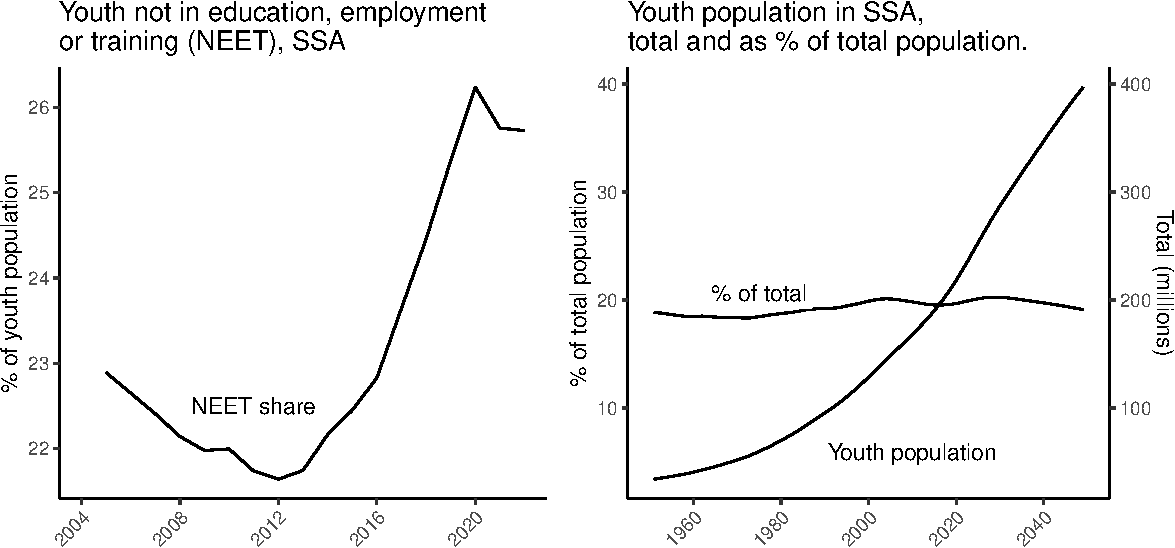
\includegraphics{figures/fig-neet-1} 

}

\caption{Demographic and economic activity trends among youth in SSA}\label{fig:fig-neet}
\end{figure}

\footnotesize

\noindent \emph{Source: Left}: \textcite{ilo2023b} modelled estimates. \emph{Right}: World Population Prospects, \textcite{unitednations2022}.
\normalsize
\hfill\break

\noindent In addition to these hurdles, youth in SSA face headwinds that beset all labor markets entrants. When employment opportunities are scarce, young applicants are generally disadvantaged relative to older workers due to their limited work experience and inability to signal their skills to potential employers \autocite{acemoglu1998}. Young workers are also more likely to find jobs in the informal sector: ILO estimates that the rate of informal employment among youth is 77 percent worldwide, significantly higher than the 61 percent among adult workers \autocite{bonnet2018}. About 83 percent of youth who enter the job market in Africa need at least one year to find employment \autocite{africandevelopmentbank2022} --- and such extended periods of unemployment have been shown to create lasting, negative wage and employment effects in both high-income economies \autocite{moller2015,petreski2016,schmillen2017,emmenegger2017} and emerging ones \autocite{tiongson2007,mojsoska-blazevski2017}. Young women are beset by additional difficulties, such as constricting social norms related to occupation type and family formation.

The detrimental effects of a faltering SWT extend beyond the economic, also encompassing social, psychological, and political dimensions. Gainful employment not only provides a means of livelihood, but also grants young individuals a sense of self-worth, dignity, and purpose, fostering their holistic development \autocite{mains2011}. High levels of youth unemployment, on the other hand, may fuel social and political instability \autocite{urdal2006}. The sheer size of the youth population in SSA, with a substantial proportion seeking employment, highlights the need for effective strategies to reduce frictions along the SWT, prevent the exclusion of youth from meaningful economic participation, and to harness their energy and potential. Given the sheer number of youth that will be embarking on informal sector careers in the coming decades, and the importance of the school-to-work transition for determining employment prospects in the long run, it is crucial that we develop a deeper understanding the mechanisms of the SWT in informal labor markets, as well as the circumstances that arise when these mechanisms are not in place. I contribute to this understanding over the three chapters of this thesis.

In a broad sense, the first chapter sets the stage by providing a cross-country comparison of youth labor markets in low- and lower-middle income countries and by examining the importance of work formality, working poverty, education quality, and other factors in determining the youth-specific strength of labor markets. My co-authors and I construct a multi-dimensional index, focusing on incorporating indicators not included in more widespread measures of labor market strength. The second and third chapters demonstrate the usefulness of longitudinal microdata for studying the SWT -- a unique and underutilized approach given the lack of such data for informal labor markets, and for SSA in general. In Chapter 2, I rely on a detailed panel dataset conducted with about 1500 youth in the urban center of Cotonou, Bénin over the course of three years to analyze transition types and identify determinants of a successful school-to-work transition. Chapter 3 relies on a matched apprentice-trainer subset of the same dataset to analyze the costs, benefits, and effectiveness of a unique apprenticeship scheme embedded in the informal sector in Bénin, and to evaluate whether informal training firms can successfully be incorporated into a national vocational education system.

In the remainder of this introduction, I present an outline of the existing methodological and empirical literature on youth labor markets in informal settings and the school-to-work transition that takes place in such labor markets. I also provide a brief synopsis of the methods and results of the three chapters comprising this thesis.

\hypertarget{the-african-youth-bulge-is-a-growing-concern-for-policy-makers}{%
\subsubsection*{\texorpdfstring{\emph{The African ``Youth Bulge'' is a growing concern for policy makers}}{The African ``Youth Bulge'' is a growing concern for policy makers}}\label{the-african-youth-bulge-is-a-growing-concern-for-policy-makers}}

In 2020, 77 percent of Africa's population was under the age of 35. Yet Sub-Saharan Africa (SSA) is projected to have the fastest population growth in the world through 2100, accounting for more than half of the global population increase by 2050 \autocite{un2022}. As a result, the \textcite{unitednations2022} projects that 400 million youth will inhabit sub-Saharan Africa by 2050 (Figure \ref{fig:fig-neet}), and constitute half of its working-age population by 2063 \autocite{africandevelopmentbank2022}. The resulting ``youth bulge'' means that youth employment in Sub-Saharan Africa (SSA) is a pressing concern for governments, civil society, and development partners alike \autocite{ilo2022a}. The potential for a ``demographic dividend'', such as that experienced by East Asia between 1965 and 1990, are limited by the fact that fertility rates in SSA are tapering off much more slowly, leaving the ratio of dependents to working-age adults unchanged \autocite{eastwood2011,filmer2014}.

Today, people between the ages of 15 and 24 account for 60 percent of the unemployed population in Africa \autocite{bonnet2018}. If progress on high-quality job creation and fertility rate reduction continues to stall, persistent youth unemployment and the proliferation of vulnerable and precarious youth employment could lead to political unrest, such as those seen during the Arab Spring \autocite{urdal2006}, as well as destabilizing waves of migration. On the other hand, a successful demographic transition supported by skills development and employment programs, as well as a sharp reduction of fertility usually accompanying economic development, would represent a massive opportunity for the continent. Thus, successful SWTs should be seen as a potential driver of much-needed economic growth, as the productive energy and innovative spirit of youth can contribute to revitalizing industries, fostering entrepreneurship, and steering the region towards a path of sustainable development \autocite{filmer2014,worldbank2019}.

\hypertarget{the-vast-majority-of-african-youth-are-employed-in-the-informal-sector}{%
\subsubsection*{\texorpdfstring{\emph{The vast majority of African youth are employed in the informal sector}}{The vast majority of African youth are employed in the informal sector}}\label{the-vast-majority-of-african-youth-are-employed-in-the-informal-sector}}

Workers in emerging and developing countries constitute 93 percent of the world's informal employment \autocite{bonnet2018}. In SSA, 95.8 percent of workers aged 15-24 are employed in the informal sector, compared to 86.6 percent of adults - in other words, adults are more than three time more likely to be employed formally \autocite{kiaga2020}. In West Africa, the informality rate among youth is as high as 97.9 percent \autocite{bonnet2018}.

Though formality rates are rising in Africa, formalization of the informal sector and formal job growth are not progressing nearly fast enough to absorb the inflow of young labor market entrants \autocite{filmer2014}. Moreover, while the rate of informal work dropped by about 5 percent between 2004 and 2019 \autocite{ilo2023}, the recovery from the Covid-19 pandemic has been characterized by a return to informal, rather than formal, work.

Employment in the informal sector is often associated with low wages, precarious working conditions, and a lack of access to social protection --- the last of which affects over 4 billion workers worldwide \autocite{ilo2023a}. According to the \textcite{africandevelopmentbank2016a}, 41 percent of working youth remain food insecure, indicating that their earnings do not cover even basic needs. Yet for the majority of youth in low-income countries, waiting for a formal employer is not an option. Those who insist on searching for a formal job, and whose families can afford it, may wait years for an opportunity to open up \autocite{serneels2007,manacorda2017}.

\begin{figure}[H]
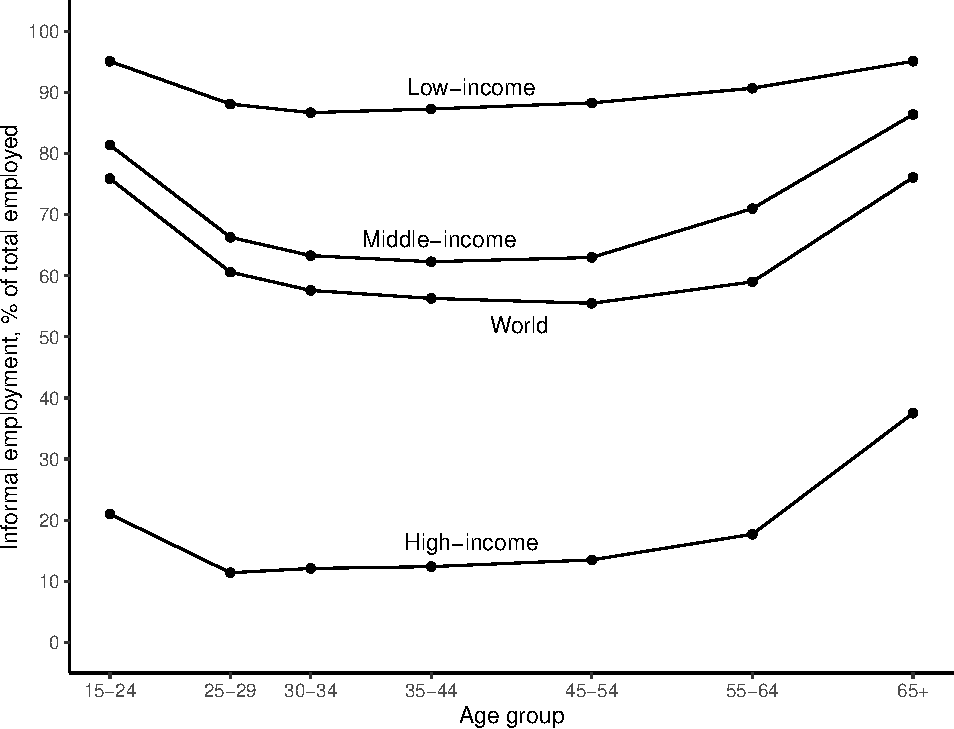
\includegraphics[width=0.8\linewidth,]{figures/fig-inf-1} \caption{Age informality profiles: world and country income groups (\%), 2019}\label{fig:fig-inf}
\end{figure}

\footnotesize

\noindent \emph{Source}: \textcite{ilo2023a} based on calculations from national household surveys from 146 countries, representing 92.6 percent of global employment.
\normalsize
\hfill\break

Figure \ref{fig:fig-inf} shows that participation in the informal sector is generally concave (or inverted U-shaped): youth enter the labor market through the informal sector, transition to formal work at increasing rates, reaching a maximum rate of about 25 percent formality between the ages of 35 and 44, and then transition back to the informal sector \autocite{chacaltana2019}. Over 360 million youth are engaged in informal employment across the globe, according to 2018 ILO estimates. In other words, youth are the most exposed to informality, at least until they near the end of the working lives.

The task for policymakers in LICs lies in putting policies in place that will allow the informal sector to flourish. This entails enacting policies that will protect workers, especially youth, from precarious or predatory working conditions, as well as providing avenues to financing, training, and market access. Additionally, it involves tackling the regulatory red tape that frequently impedes the smooth operation of informal enterprises \autocite{imf2017}.

\hypertarget{indices-are-a-useful-tool-for-comparative-studies-of-youth-labor-markets}{%
\subsubsection*{\texorpdfstring{\emph{Indices are a useful tool for comparative studies of youth labor markets}}{Indices are a useful tool for comparative studies of youth labor markets}}\label{indices-are-a-useful-tool-for-comparative-studies-of-youth-labor-markets}}

An unbiased appraisal of the functioning of youth labor markets are critical for understanding the SWT and drafting constructive policy, and there is a general consensus that the measurement of labor market strength needs to incorporate a range of indicators that reflect both supply factors (the preparedness of youth for work) as well as demand factors (the demand of firms for youth labor). The ILO has led the empirical study of labor market dynamics, notably with the introduction of its 18 Key Indicators of the Labor Market (KILM). This set of measures encompass employment factors (status, sector, occupation, and work hours), labor conditions (wages and working poverty), as well as socioeconomic data related to the job seekers, including their education and labor productivity \autocite{ilo2016}. Further work focused on reformulating the KILM indicators to better capture labor market dynamics for the youth population \autocite{elder2010}; however, being derived from household surveys rather than national indicators, these served as approximations rather than direct measurements of labor markets.

While providing valuable insights into the functioning of labor markets, these sets of indicators fell short of providing a coherent picture of youth labor market strength. The introduction of the KOF Youth Labor Market Index \autocite{renold2014,pusterla2015,pusterla2016} addressed this gap by combining a new set of indicators into a single number, in a similar spirit to the Human Development Index \autocite{sudhir1994}. These studies offer valuable insights into labor market conditions for youth in high-income countries, but are poorly equipped to describe low-income economies, both due to the appropriateness and the availability of the included indicators.

Similar youth-centric indices have been introduced in the wake of the YLMI which have aimed to capture youth quality-of-life more generally. The Youth Development Index combines 18 measures of youth education, health and well-being, employment opportunity, and political and civic participation to rank 183 countries \autocite{sen2016}. The Youth Progress Index combines 60 indicators to measure a similar concept, but explicitly excludes economic variables to allow for comparisons with GDP \autocite{lisney2018}. Both indices suggest that youth well-being is very tightly correlated with per-capita income, especially at lower income ranges, but they do not share our explicit focus on labor market outcomes.

\hypertarget{study-of-the-school-to-work-transition-is-aided-by-longitudinal-data}{%
\subsubsection*{\texorpdfstring{\emph{Study of the school-to-work transition is aided by longitudinal data}}{Study of the school-to-work transition is aided by longitudinal data}}\label{study-of-the-school-to-work-transition-is-aided-by-longitudinal-data}}

Both cross-sectional and longitudinal data have been used to quantify the onset and duration of the school-to-work transition. The use of cross-sectional data, which is more widely available, involves the comparison of the age at which a certain proportion of the population has left school (50 percent or 75 percent, depending on the study) to the age at which the same percentage of the population has found a job. In essence, this reflects the average SWT transition for the population \autocite{nilsson2019}. \textcite{quintini2014} employ this approach to report transition duration, along with mean school-leaving age and age at first employment, showing that youth in emerging countries experience longer transitions and leave education earlier, while also experiencing higher rates of inactivity. This literature suggests that there is frequent job turnover among younger workers who engage in a search process of ``shopping around'' temporary jobs until they settle on a career path. In emerging economies, the informal sector employment appears to play a similar, transitory role, though it appears be used as a substitute for skills formation to a greater degree than in high-income economies \autocite{cunningham2008,bosch2010}.

\textcite{nilsson2019} argues that the use of cross-sectional data to quantify the SWT rests on a number of unrealistic assumptions, however. First, the calculation assumes that every individual in the population attends school, secures employment, and remains continuously employed upon labor market entry \autocite{ohiggins2008}. As a result, transitions that include a long period of economic inactivity after school-leaving -- a very common occurrence in low-income contexts, especially for women -- are not accurately represented in the statistic. Similarly, cross-sectional data covers multiple cohorts, making a measure of transition duration only meaningful in a stationary labor market, i.e.~one in which there are no differences in transitions between cohorts. Finally, official employment statistics often overlook large parts of the informal economy.

These issues can be addressed by using job history and panel data, which allows for the computation of transition duration for each individual. However, since most samples will include ongoing or incomplete transitions, aggregating individual transitions still yields a biased estimate of the SWT duration. This limitation can be alleviated in turn by employing survival analysis to estimate the likely transition duration for right-censored observations. A body of literature has emerged employing this approach to study SWTs in emerging countries \autocites[e.g.][]{khan2013,nordman2015,manacorda2017}.

Detailed panel and job history data can also be used in combination with Optimal Matching Analysis (OMA) to yield unique insights into the school-to-work transition of a population. OMA is a statistical method that calculates a metric indicating the relative similarity between individual sequences of school-to-work transitions, allowing for the sorting of similar sequences into groups by similarity \autocite{elzinga2003}. A body of literature applies OMA school-to-work transitions in various high-income countries \autocite{schoon2001,mcvicar2002,brzinsky-fay2007,quintini2009,brzinsky-fay2014,brzinsky-fay2016,middeldorp2019}. One recent study has used Optimal Matching in a cross-country study of SWTs in low- and lower-middle income countries \autocite{pesando2021}, while the only other examples of OMA using data from LMICs are a study of the distance between experienced and ideal interpersonal relationships in Malawi \autocite{frye2015}, family planning (also in Malawi, \textcite{furnas2016}), and time usage among the elderly in South Africa \autocite{grapsa2016}.

\hypertarget{tvet-in-informal-firms-and-the-promise-of-dual-system-training}{%
\subsubsection*{\texorpdfstring{\emph{TVET in informal firms and the promise of dual system training}}{TVET in informal firms and the promise of dual system training}}\label{tvet-in-informal-firms-and-the-promise-of-dual-system-training}}

The current generation of Africans is the most educated yet (\textcite{filmer2014}), yet many find that the promise of stable and gainful employment does not follow. Moreover, despite increasing educational attainment, the quality of education remains critically low in many countries in SSA \autocite{worldbank2018}, and does not translate in to measurable improvements in marketable skill levels \autocite{filmer2020}. Many follow their parents into informal work, and find that despite their best efforts in school, their employment prospects are similar to those of their parents.

Technical vocation education and training was a high priority for many bilateral and multilateral agencies in the 1960s and early 1970s. The World Bank funded many projects to promote TVET, and the ILO published a number of influential reports on the importance of training for the informal sector \autocite{palmer2007}. For recipient governments, integrating TVET into their modernization strategies was a logical step, achieved through the incorporation of vocational elements into secondary education and establishing national industrial and vocational training centers, often with the backing of the ILO. Throughout the 1980s, however, structural adjustment policies took the focus away from public education and training. The World Bank spoke out in favor of primary education over vocational training, undermining the rationale for external assistance for TVET \autocite{king2007}.

In recent years, the youth employment crisis and rising rates of primary education attainment has generated renewed interest in TVET as a post-primary educational path. Providing quality post-primary education to all children and youth in low- and lower-middle-income countries with growing populations is a significant challenge. In SSA, the completion rate of upper secondary education increased by only 3.4 percentage points during the past decade, from 23.3 percent to 26.7 percent, leaving the region furthest behind in an international comparison \autocite{un2022}. In many low-income countries, both politicians and policy experts are drawn to the potential of TVET to reduce unemployment through by equipping youth with practical and job-specific skills.

Taking an example from Germany, Switzerland, and other European countries, several governments have begun implementing a training system that leverages the immense potential of the informal sector by coupling informal firms with classroom education. In the so-called dual system, apprentices develop practical skills via on-the-job training while acquiring relevant theoretical knowledge and extending their general education at vocational training institutions. Such schemes show promise in fulfilling the fundamental goal of education: the promotion of literacy, numeracy, and socioemotional skills among its youth, even while preparing them for the challenges of the labor market \autocite{arias2019}. As these types of programs are still a novelty in most low-income countries, their place in the broader education system, effectiveness, and challenges are still in the process of being defined \autocite{igarashi2018}.

Only one study has attempted a full-fledged impact evaluation of dual-system training in Sub-Saharan Africa. In a random experiment involving an apprenticeship scheme that combined 12 to 24 months of on-the-job training with classroom training in local vocational training centers, \textcite{crepon2019} found that participating youth earned 15 percent more after three years and contributed to more complex and non-routine tasks at their training firms. They also graduated and received formal certification of their training at a higher rate than youth who did not participate in classroom training. In this thesis, I study the effectiveness of the \emph{Certificat de Qualification Professionnelle} (CQP), in which youth similarly attend classroom education once a week while participating at an otherwise traditional apprenticeship.

\hypertarget{contribution-and-structure-of-dissertation}{%
\section{Contribution and Structure of Dissertation}\label{contribution-and-structure-of-dissertation}}

This thesis was completed under the auspices of the research project \textbf{LELAM-TVET4INCOME}, funded by the Swiss National Science Foundation. This program addresses a crucial knowledge gap regarding the connection between TVET and youth labor markets. Examining case studies and collaborating with partner institutions in four countries ---- Benin, Chile, Costa Rica, and Nepal -\/--- analyze the connection between education and employment, as well as youth labor market dynamics, across countries at various stages of economic development. Additionally, the goal of the project is to assess the impact of reforms, interventions, and policies in these countries through rigorous empirical evaluation. The central, guiding question of this research program is a fundamental question: what are the necessary and sufficient conditions under which TVET can enhance youth income? Towards this end, the project has outlined four specific research questions that provide a structured framework, two of which I investigate in greater detail in my thesis:

\begin{enumerate}
\def\labelenumi{\arabic{enumi}.}
\tightlist
\item
  How can we measure the youth labor market situation in low and middle income countries?
\item
  Does improving the linkage between the actors of the education and employment system reduce unemployment, improve gainful employment, job quality, and thus income of the youth?
\end{enumerate}

\noindent In \textbf{Chapter 1: Youth Labor Index for Low Income Countries}, co-authored with Erwin Lefoll and Dr.~Isabel Günther, we construct and analyze the eponymous Youth Labor Market Index for Low-Income Countries, or YLILI. The YLILI provides a more nuanced evaluation of labor strength than the two most commonly used indicators, namely average income and employment rate. The index comprises 10 indicators grouped into three dimensions: transition, working conditions, and education, using data sourced from public domain and provided by the International Labour Organization (ILO), the World Bank, and UNESCO.

The results reveal a wide variation of youth labor market strength across the 54 (out of 79) low-income and lower-middle income countries for which data is available. The strongest youth labor markets among these countries are concentrated in Central Asia, while labor markets in SSA are generally much weaker than those in South America and South and Central Asia. The highest variation is observed within the education dimension, namely for the share of youth without any secondary education, the youth literacy rate, and a set of harmonized test scores. Thus, the quality of the education system is an important driver of the rankings generated by the index. Our analysis also tests various hypotheses regarding the macroeconomic and demographic drivers of the YLILI ranking. Strikingly, we find that the fertility rate - which essentially captures the lagged severity of the youth bulge in a country population - is the strongest tested predictor of YLILI. High rates of child-bearing decrease the levels of economic activity and educational attainment among the female population, while adding pressure to the already overburdened educational systems in countries with a high youth-to population ratio at the same time.

The YLILI emphasizes that the youth employment crisis is multifaceted, and policy responses should be tailored to the specific strengths and weaknesses of each country's youth labor market. To facilitate this, we make the index available in the form of an interactive webtool (\href{https://nadel.shinyapps.io/ylili}{https://nadel.shinyapps.io/ylili/}), which allows policymakers to clearly visualize the issues that are in most need of being addressed. Finally, in light of the 25 countries that were entirely missing from our index, an important lesson from the paper is the importance of consistent collection of labor market indicators on the one hand, and the publication of these indicators in age- and gender-disaggregated form on the other.

\todo{1}\hl{This author and Dr. Isabel Günther played major roles in conceptualizing the study. Erwin Lefoll was fully responsible for initial data collection, visualization, statistical analysis, and the first draft of the manuscript. This author revised the analytical approach, conducted robustness checks, and developed the accompanying web-based tool. Dr. Isabel Günther had a leading role in revising the analytical strategy and interpreting results.}

In \textbf{Chapter 2: Lost in Translation: School-to-Work Transition Mapping in Urban Bénin}, I shift perspective to focus on school-to-work transitions in a single urban labor market in the West African country of Bénin. Over three years, I gathered detailed data on the education and labor market activity of a sample of 752 youth living in the country's economic largest center, Cotonou. Employment histories dating back seven years form the backbone of the analysis, and track youths paths through five activity states: \emph{School}, \emph{Apprenticeship}, \emph{Wage Employment}, \emph{Self-Employment}, and \emph{NEET}.

In order to better understand the dynamics of the SWT in this highly informal economy, I use a variety of methodologies to analyze these employment histories. First, I characterize the periods of school-leaving and labour market entry for the youth in the sample. Deducing the age of the respondent at each point of their observed employment history allows me to calculate the age at which youth complete their schooling and transition to their first job, as well as the duration of this transition, and a wealth of socioeconomic and family characteristics allows me to identify factors that influence the time it takes for youth to enter the labour market. In a second approach, I follow \textcite{bosch2007} and \textcite{cunningham2011} in considering the employment histories as continuous Markov processes. This allows me to study the flows between different activity states over the course of the entire SWT. Moreover, by separating the probability to transition between two states from the likelihood that a youth exits a particular state in the first place, I am able to compare the transition probabilities for age and gender subgroups. Finally, I apply optimal matching analysis (OMA), a technique used to identify similarities in sequences, to identify shared patterns in the SWT trajectories experienced by youth, and group them into clusters of like transitions.

The conclusions of the paper challenge several assumptions about highly informal, urban labor markets. First, the mean school-leaving age is over 23 and a half years, which more closely resembles the graduation age of high-income countries than that reported in official statistics for Bénin - indicating a massive gap in educational attainment between rural and urban areas. Second, OMA indicates that transition paths are relatively stable -- only a small fraction of youth exhibit a transition type that is not dominated either by education, self-employment, wage employment, or inactivity. Third, we find that female labor market participation, as measured by the probability to exit the SWT (i.e., to find employment), is considerably lower than implied by recent studies at the national level. Young men exit the SWT at a rate of 65 percent in our sample, compared to just 47 percent of women. This finding is supported by the OMA approach, as the cluster dominated by NEET activity states is comprised almost exclusively of young women who become separated from the labor market at a young age. The study reveals the potential of longitudinal surveys tracking youth labor market activities, though I argue that longer histories with more than five activity states would allow for even more informative grouping of transition types.

In \textbf{Chapter 3: Costs and Benefits of Dual Education in the Informal Sector}, co-authored with Dr.~Sylvain Kpenavoun, Dr.~Esaïe Gandonou, Dr.~Guy Nouatin and Dr.~Rubain Bankole, I analyze the effectiveness of a unique apprenticeship program in Bénin called \emph{Certificat de Qualification Professionnelle} (CQP). The program builds on existing apprenticeships in the informal sector by adding a weekly classroom training session. We utilize a unique dataset tracking earnings and employment data for 427 apprentices participating in the program, as well as matched survey data from interviews conducted with the master craftsmen from the total of 197 small firms in which the training took place.

The CQP program has two interrelated goals. On the one hand, meta-analyses of the training literature show that programs combining hands-on training with classroom teaching are the most effective at improving youth employment outcomes \autocite{kluve2019,ghisletta2021}. On the other hand, the size of the informal sector and limited offering and access to formal technical and vocational education and training (TVET) combine to make informal training play a central role in the preparation of youth for the labor market. Given the prohibitive cost and political frictions that would be involved in a forced formalization of informal sector training, a program that implements a modicum of formalization measures, such as enforced written contracts, coherent training curricula, clear learning objectives, and a nationally-recognized certificate, is an important stepping step towards integrating informal training schemes into the national, formally recognized TVET system.

The paper makes two important contributions to the literature on informal training. First, we contrast the efficacy of dual system training to informal apprenticeship without a classroom education component. Second, we evaluate the costs and benefits of the program for both participating apprentices and their training firms.

We find that, after three years of training, apprentice scores on trade-specific competence measures increase by .13 standard deviations, while their trainers' assessment of their competence and experience on a series of sector-specific tasks increased by 0.46 SDs and 0.58 SDs, respectively. However, it is not possible to distinguish the learning outcomes of the CQP participants from those of comparable apprentices who did not participate in supplemental classroom training. Cost and benefits calculations for all apprentices indicate that apprentices receive more in allowances from their trainers, including food, transport, and ``pocket money'', than they pay in fees, whereas the net costs for firms are highly dependent on the productive contributions of the apprentices (and how they are measured).

\todo{1}\hl{The author of this dissertation conceptualized the study, developed the analytical strategy, and interpreted the results, with the invaluable input of Drs. Esaïe Gandanou, Guy Nouatin, and Sylvain Kpènavoun Chogou. Dr. Sylvain Kpènavoun Chogou orchestrated data acquisition, including surveyor training and data quality checks. Dr. Rubain Bankole led additional qualitative surveys during the later phases of the project and aided in the interpretation of the results.}

\newpage
\markboth{References}{References}
\printbibliography[segment=\therefsegment,heading=subbibintoc,title={References}]

\newsection

\chapter{Youth Labor Index for Low Income Countries}

\emph{co-authored with Erwin Lefoll \& Isabel Günther}

\begin{chapabstract}
This paper introduces the Youth Labor Index for Lower-Income Countries (YLILI), a composite index of 10 labor market indicators specifically tailored to developing countries. The indicators are chosen based on their relevance for economies with high levels of informal work and because they can be computed for ages 15-24 and disaggregated by gender. The index rankings suggest that poor education outcomes and high working poverty rates are the main drivers of weak youth labor market outcomes, especially in sub-Saharan Africa. Labor market scores are higher for males, a result driven by the large shares of young women not in education or the workforce. The fertility rate is a strong predictor of index scores, suggesting that countries with fastest growing youth populations are also struggling to provide sufficient opportunities for decent youth employment. A webtool allows users to explore the YLILI and identify policy priorities.
\end{chapabstract}

\newpage

\hypertarget{introduction}{%
\section{Introduction}\label{introduction}}

Over the past three decades, the global share of youth residing in developing countries has increased by 20 percentage points, to a little over 50 percent of all youth in 2020 \autocite{unitednationsdevelopmentprogramme2019}. This share is expected to continue to rise, and with it the number of young workers entering the workforce \autocite{roser2019}. Lacking formal employment opportunities and facing unemployment without social security, youth in many low-income countries (LICs, as classified by the \textcite{worldbank2020a}) and lower-middle income countries (LMICs) must resort to work that is irregular, underpaid, and lacking in benefits or advancement opportunities. Few can afford to be inactive for extended periods of job search after leaving school. In sub-Saharan Africa (SSA), where 40 percent of inhabitants are under the age of 15 and where youth population growth is outpacing formal job creation by a large margin, the ``youth employment crisis'' is increasingly also being seen as a ``missing jobs'' crisis \autocite{sumberg2021}. Long unemployment spells reduce productive capacity in later life, curtailing youths' earnings potential and dampening the growth prospects of the economy \autocite{gregg2005}. In the worst case, persistent difficulties in transitioning to gainful work can drive youth to political unrest and violence, as has been the case in the Middle East \autocite{urdal2006}.

The UN has addressed this issue with its 8th Sustainable Development Goal (SDG)---full and productive employment and decent work for all, with particular emphasis on youth (and other vulnerable populations). Unfortunately, the productivity and decency of work does not lend itself to easy measurement. The unemployment rate is the most widely-used indicator for evaluating labor market strength, but it is largely uninformative in many developing countries, where low savings rates and the lack of social insurance force youth to accept underpaid, unskilled work. In such an environment, rather than indicating widespread ``decent'' work, low unemployment rates reflect that large segments of the youth population simply cannot afford \emph{not} to work \autocite{zimmermann2013,dewan2007}. Thus, to better analyze and compare youth labor markets in developing countries, a more multifaceted indicator than the unemployment rate is needed.

To this end, this paper presents the Youth Labor Index for Lower-Income Countries (YLILI)---a composite index of 10 youth labor market indicators specifically tailored to the realities of work in low- and lower-middle income countries and organized around three central themes: youth transition to work, working conditions for youth, and human capital. The YLILI builds on a related index compiled by the Swiss Economic Institute (KOF), but relies on indicators that are more relevant to and available for low-income countries. Specifically, the unemployment rate is replaced by indicators more appropriate for the measurement of highly informal economies.

A measure of youth labor market strength will ideally be youth-specific rather than pertaining to the working-age population as a whole. Youth and adults face qualitatively different conditions and obstacles on the labor market. For one, youth often experience worse outcomes than adults: according to the latest ILO statistics for LICs and LMICs, for instance, they were 20 percent (3.2 percentage points) more likely to be among the working poor and 13 percent more likely to be underemployed \autocite{ilo2023b}. Rapid demographic and structural change also imply generational differences in the nature of work: youth face stiffer competition due to growing populations, are more likely to migrate to urban areas \autocite{debrauw2014}, and are increasingly eschewing the agricultural work of their parents and grandparents \autocite{honorati2016}. All indicators used in the YLILI are thus disaggregated by age group, covering youth aged 15--24 specifically, and include youth-specific measures such as school test performance. Disaggregation by gender allows for further analysis. Current data availability allows us to generate an overall YLILI score for 54 (out of 79) low- and lower-middle income countries. An accompanying online tool (\url{https://nadel.shinyapps.io/ylili}) allows users to view each index component in detail and compile the ranking according to custom parameters.

The YLILI suggests that, among low-income and lower-middle income countries, youth labor markets perform best in Europe and Central Asia. Meanwhile, 18 of the 20 worst-performing countries are located in SSA (Pakistan and Afghanistan being the two exceptions). The poor performance in SSA is driven primarily by high working poverty rates and low scores on measures of education. In general, education outcomes are found to vary the most across countries, and as such are the main driver of the final index rankings. Perhaps our most striking finding is that demographic patterns best predict the YLILI scores: countries with large youth populations and high fertility rates tend to perform worse on the YLILI index, particularly in the transition and education dimensions. This suggests a compounding of unfavorable demographic and labor market conditions for youth, with the highest numbers of youth entering labor markets with scarce opportunities. Thus, we conclude that prospects for youth in the poorest countries are unlikely to improve until fertility and dependency rates fall substantially. Finally, we examine differences in YLILI scores for young men and women and find that high female inactivity rates and substantial education deficits drive the observed gender gap, particularly in countries that perform poorly on the YLILI overall.

The remainder of the paper is structured as follows. Section \ref{indicators} describes the indicators of the YLILI and the data. Section \ref{methods} describes how the indicators are combined to generate the YLILI country score. Section \ref{yliliresults} presents some applications of the YLILI, including regional analysis and a breakdown by gender. Section \ref{robustness} presents several robustness checks, and highlights potential limitations. Section \ref{discussion} concludes and discusses some policy implications.

\hypertarget{indicators}{%
\section{The YLILI Indicators}\label{indicators}}

Composite indices help make complex and multidimensional phenomena more tractable by combining multiple measures into country-specific \emph{ranks} or \emph{progress indicators}, which in turn allow for easier comparisons across countries and over time. Thanks to their simplicity, they are often instrumental in rallying attention to an issue in policy or governance, such as corruption (the Corruption Perceptions Index), human well-being (Human Development Index, HDI) or the business environment (Ease of Doing Business Index). In some cases, indices are also used to bring attention to the misuse of a popular indicator in public discourse. In the case of the HDI, a combination of life expectancy, education and income indicators was proposed as an alternative to GDP as a measure of a country's level of development \autocite{undp1990}.

The YLILI is inspired by the Youth Labor Market Index (YLMI), a composite index introduced in 2014 by the Swiss Economic Institute (KOF) and updated annually every year since \autocite{renold2014}. The YLMI is composed of 12 indicators and has helped highlight issues such as the \emph{youth paradox}---unprecedented educational attainment going hand-in-hand with rising youth unemployment in many high-income countries. However, the YLMI's heavy sourcing of data from the EU and OECD means its usefulness is limited to the study of youth labor markets in high-income countries \autocite{pusterla2015,pusterla2016}. Crucially, the index relies heavily on the unemployment rate, a widely-cited indicator that is much more informative in high-income than low-income contexts. Unemployment rates in the poorest countries regularly fall under 5 percent, but rather than indicating well-functioning labor markets, they remain low because social security systems are weak and informal, and most people simply cannot afford to remain idle \autocite{filmer2014}. Families with low savings are unable to support graduates through an extended job search, leaving young people with no choice but to enter own-account employment or poorly-paid jobs below their skill level \autocite[margolis2014]{fields2012}, predominantly in the informal sector \autocite{herrera2013,sengenberger2011}.

Economic development tends to go hand in hand with the formalization of work \autocite{laporta2014}---about 90 percent of employed youth in developing countries work in the informal sector on average, compared to less than 20 percent in high-income countries \autocite{bonnet2018}. Formal work comes with many benefits, from higher wages to employment stability and social security coverage. Thus, the fact that among LICs and LMICs, \emph{lower} unemployment rates tend to be associated with \emph{higher} rates of informal work---in contrast to rich countries---presents a problem for the unemployment rate as a measure of economic health (Figure \ref{fig:fig-infunemp}. An indicator that can mean opposite things depending on development level violates a key assumption of composite indices, namely that each of the constituent indicators provides a well-ordered ranking of performance.

\todo{4}\hl{The negative correlation between the unemployment rate and job quality/formality in low-income countries highlights the importance of considering alternative indicators such as the NEET rate to assess youth disengagement and labor market dynamics. Unlike the unemployment rate, the NEET rate encompasses a broader range of activities beyond just employment, including education, training, and other forms of non-participation, and does not exhibit a negative correlation with informal work in LICs and LMICs (Figure }\ref{fig:fig-infneet} \hl{in Appendix A2). For this reason, we exclude the unemployment rate from the YLILI and rely on the NEET rate instead.}

\begin{figure}[H]
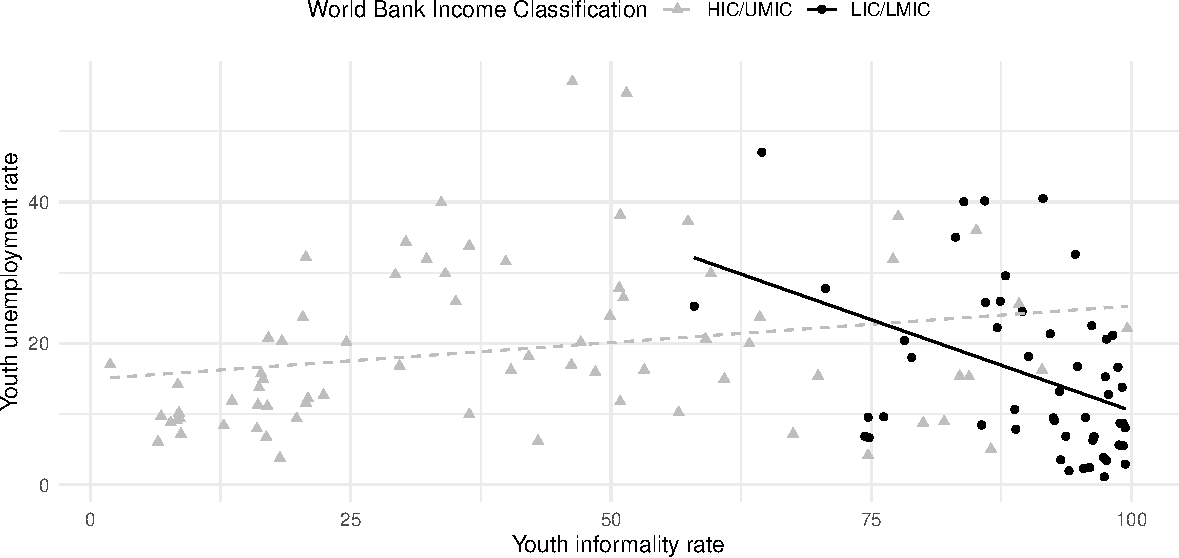
\includegraphics{figures/fig-infunemp-1} \caption{Relationship between youth unemployment and informality by income level}\label{fig:fig-infunemp}
\end{figure}

In addition to the unemployment rate, the relaxed unemployment rate (the share of unemployed and discouraged workers relative to the size of the labor force), the relative unemployment rate (ratio of youth to adult unemployed) and the long-term unemployment rate (share of unemployed who have been continuously unemployed for a year or more) are all included in the KOF YLMI and pertain directly to the unemployment rate. We exclude these indicators from the YLILI as well, and replace them with measures that are more relevant for describing labor market conditions in low-income economies. For instance, the working poverty rate (living on less than \$1.90 a day) and the literacy rate are generally close to zero for high-income countries (and thus not part of the YLMI), but vary meaningfully for low-income countries. Table \ref{tab:tbl-kofcomp} in Appendix B2 provides a more detailed overview of the similarities and differences between the YLMI and YLILI.

We stipulate four conditions that an indicator must fulfill to be included in the YLILI. First, the indicator must be a monotonic increasing function of labor market performance. This means that it must be clear whether a higher value of an indicator is always preferred to a lower one (i.e., the higher, the better) or vice-versa. From the perspective of a policy-maker, it must be possible to rank the indicator from the worst to the best outcome. Second, the indicator must be disaggregated by different age groups, and specifically must be available for the 15 to 24 age group. Third, the indicator must be desegregated by sex. Fourth, indicator estimates must be available for at least half of the LMICs and LICs dating back no further than 2010. We limit ourselves to indicators from four reputable compilers of international statistics: ILOSTAT, UNESCO, the World Bank, and the Demographic and Health Surveys (DHS). We retain indicators for which data is available for at least one year since 2010 for 40 or more low-income and lower-middle income countries (as of April 1st 2021, there were 79 LMICs and LICs combined according to the \textcite{worldbank2020a}).

Ultimately, we identified ten indicators that meet these conditions. We classified these into three broad dimensions that best reflect, in our view, youth labor markets in developing countries: transition from education to the labor market, working conditions, and educational background (Table \ref{tab:tbl-indicators}). On the demand side, the transition dimension reflects economic participation and the smoothness of the transition from education to the workplace, whereas the working conditions dimension captures the quality of work. The final dimension (education) focuses on the supply side of the labor market, i.e., the skill level of job seekers. Ultimately, indicators were chosen as much based on data availability as desirability; nevertheless, it is worth noting that as with any composite index, the final choice and weighting of indicators is a value-laden interpretation of the authors. A corresponding webtool (\url{https://nadel.shinyapps.io/ylili}) allows users to fine-tune the index to their preference and to test the robustness of the final rankings presented here. For more details on the availability of each indicator, see Appendix B2.

\begin{singlespacing}
\begin{singlespace}
\begin{table}[H]
\caption{\textrm{\normalfont \small Overview of Indicators \label{tab:tbl-indicators}}}
 \centering
 \scalebox{0.75}{
\begin{tabular}{c c l c c c}
& & & & & \\
\hline \hline
& \multicolumn{2}{c}{\multirow{2}{*}{Indicator}} & \multicolumn{1}{c}{\multirow{2}{*}{In KOF YLMI}} & \multicolumn{1}{c}{\multirow{2}{*}{Source}} & \multicolumn{1}{c}{\multirow{2}{*}{Self-computed}} \\
& & & & &   \\
\cline{2-6}
\parbox[t]{2mm}{\multirow{14}{*}{\rotatebox[origin=c]{90}{\underline{Demand}}}} & \parbox[t]{2mm}{\multirow{6}{*}{\rotatebox[origin=c]{90}{Transition}}} & Share not in employment & \multirow{2}{*}{\ding{52}} & \multirow{2}{*}{ILOSTAT} & \multirow{2}{*}{No} \\
& & education, or training (NEET) & & &  \\
& & \multirow{2}{*}{Relative working conditions ratio} & \multirow{2}{*}{{\ding{53}}} & \multirow{2}{*}{ILOSTAT} & \multirow{2}{*}{Yes} \\
& & & & &   \\
& &  \multirow{2}{*}{Skills mismatch rate} & \multirow{2}{*}{{\ding{52}}} & \multirow{2}{*}{ILOSTAT} & \multirow{2}{*}{Yes} \\
& & & & &   \\
\cline{2-6}
& \parbox[t]{2mm}{\multirow{8}{*}{\rotatebox[origin=c]{90}{Working Conditions}}} &  \multirow{2}{*}{Working poverty rate} & \multirow{2}{*}{{\ding{52}}} & \multirow{2}{*}{ILOSTAT} & \multirow{2}{*}{No} \\
& & & & &  \\
& & Time-related & \multirow{2}{*}{\ding{53}} & \multirow{2}{*}{ILOSTAT} & \multirow{2}{*}{No}  \\
& & underemployment rate & & &  \\
& &  \multirow{2}{*}{Informal employment rate} & \multirow{2}{*}{{\ding{53}}} & \multirow{2}{*}{ILO} & \multirow{2}{*}{No} \\
& & & & &  \\
& & Share in elementary & \multirow{2}{*}{\ding{53}} & \multirow{2}{*}{ILOSTAT} & \multirow{2}{*}{Yes}  \\
& & occupations & & &  \\
\cline{2-6}
\parbox[t]{2mm}{\multirow{6}{*}{\rotatebox[origin=c]{90}{\underline{Supply}}}} & \parbox[t]{2mm}{\multirow{6}{*}{\rotatebox[origin=c]{90}{Education}}} &  Share of youth with no & \multirow{2}{*}{\ding{53}} & \multirow{2}{*}{DHS} & \multirow{2}{*}{Yes} \\
& & secondary education & & &  \\
& & \multirow{2}{*}{Illiteracy rate}  & \multirow{2}{*}{\ding{53}} & \multirow{2}{*}{UNESCO} & \multirow{2}{*}{No}  \\
& & & & &  \\
& & \multirow{2}{*}{Harmonized test scores}  & \multirow{2}{*}{\ding{53}} & \multirow{2}{*}{World Bank} & \multirow{2}{*}{No} \\
& & & & &  \\
\hline \hline
\multicolumn{6}{p{\textwidth}}{\textit{Notes}: Self-computed indicators are calculated by the authors from two or more raw indicators.}
\end{tabular}}
\end{table}
\end{singlespace}
\end{singlespacing}

\hypertarget{transition-from-education-to-the-labor-market}{%
\subsection{Transition from Education to the Labor Market}\label{transition-from-education-to-the-labor-market}}

The transition category captures quantity adjustments of youth labor in developing countries. The share of youth Neither in Employment nor in Education or Training (NEET) captures the level of inactivity in the youth population, while the youth skills mismatch characterizes the degree to which the supply of youth skills meets employer demand. The relative working conditions ratio is an adaptation of the relative unemployment ratio, and compares labor market outcomes of youth to those of older workers without relying on unemployment rates.

The \textbf{share of youth NEET} captures the percentage of people aged between 15 and 24 years old who are neither in employment nor in education and training (data obtained from ILOSTAT). Hence, it refers to individuals fulfilling two mutually inclusive conditions: (i) they are not employed (i.e., are unemployed, discouraged, or inactive), and (ii) have not received any education or training in the four weeks preceding the survey \autocite{elder2015a}. Young people in education include those attending full-time or part-time education, but exclude those in non-formal education and in educational activities of very short duration \autocite{oecd2019}. Both formally and informally employed youth are considered to be working, and are thus not counted among NEET youth. Average NEET rates are given in Table \ref{tab:tbl-indicators} and shown graphically in Figure \ref{fig:fig-transitionmap} in Appendix B2. The NEET rate does not track national income in a linear manner: about 28 percent of youth in lower-middle income countries are NEET, while this rate is closer to 20 percent in both upper-middle and low income countries. High income countries have much lower youth inactivity rates, with just 11 percent youth NEET on average.

\todo{4} \hl{In general, there is a positive correlation between NEET status and the youth unemployment rate, as both indicators reflect aspects of labor market participation and opportunities for young people. Higher levels of unemployment are likely to coincide with higher levels of NEET status, indicating a lack of employment opportunities and potentially other barriers to participation in education or training. However, factors such as the availability of education and training opportunities, economic conditions, social policies, and cultural norms can influence the relationship between NEET status and unemployment rates. In LMICs and LICs, NEET rates track poor labor conditions more consistently than high youth unemployment rates, as they include discouraged work seekers and reflect the availability of education and training opportunities.}

The \textbf{relative working conditions ratio} pertains to the difference in two aspects of work quality between youth and adults (aged 25+ years old): the working poverty rate and the time-related underemployment rate. The working poverty rate is expressed as the percentage of workers living below US\$1.90 PPP. The time-related underemployment rate captures the proportion of working youth who are able and willing to increase their working hours and who are working under a threshold number of hours for a reference period. This threshold is determined separately by each country based on national circumstances.

The relative working conditions ratio indicator measures the degree to which working conditions differ for youth and adult workers, and thus captures whether youth enjoy labor conditions that are ``typical'' for their country. Youth suffering from substantially lower working conditions than the adult working population would suggest that youth engage in different jobs or tasks than adults and indicate a slower transition to decent work. We self-compute it using data from ILOSTAT as follows:

\footnotesize

\[ \text{Relative WC ratio}= \frac{\displaystyle{\frac{\text{Youth work. poverty rate}}{\text{Adult work. poverty rate (25+)}}} + \displaystyle{\frac{\text{Youth time-related unmp. rate}}{\text{Adult time-related unmp. rate (25+)}}}}{2} \]
\normalsize
\vspace*{5pt}

The closer the youth and adult rates, the more the ratio tends to one, suggesting equality in working conditions between youths and adults. Taken separately, the two components of this indicator (working poverty and the underemployment rates) tend to unity in the ideal case: when youth and adult conditions are similar. Jointly, the indicator needs to be interpreted cautiously, as a ratio above one (favoring adults) can be counterbalanced by a ratio below one (favoring youth), creating the impression of equality between generations where there is none. Youth in developing countries are about 20 percent more likely to belong to the working poor than adults, and about 13 percent more likely to face time-related underemployment. Working poverty and underemployment are higher in LICs and LMICs than higher income countries, while the differences (ratios) between youth and adult outcomes tend to be lower in relative terms.

\textbf{Job mismatch} is the third and final indicator in the transition dimension and refers to the difference between a worker's skill level and the level required by their employer. It accounts for two situations: (i) workers who are constrained to accept jobs for which they are overqualified or that do not match their skills/training and (ii) workers who hold jobs for which they are not qualified. Since the mid-1990s and the advent of the United Nation's Millennium Development Goals at the beginning of the 21st century, grass-roots approaches to solving poverty have mainly focused on improving the supply side of the labor market, i.e., making job-seekers more educated and skilled, and not the demand side, i.e.~making new and/or better jobs available \autocite{amsden2010,gore2010}. As a result, large numbers of over-qualified workers unable to take full advantage of their skills are common in many LMICs and LICs \autocite{handel2016}.

There are several ways to measure mismatch. One is to calculate the difference between the highest level of education attained and the dominant level of education observed for the worker's occupation \autocite{herrera2013}. Unfortunately, such an indicator is not available and cannot be computed using aggregated data. Our solution is to mirror the skills mismatch indicator used in the KOF YLMI, which utilizes the unemployment rate at different levels of education. This indicator captures the extent to which workers with a certain level of education are more or less affected by unemployment than others. Because this indicator is unavailable as such, we compute it manually using unemployment data disaggregated by age and level of education from ILOSTAT as follows:

\footnotesize

\[\text{Skills mismatch rate}= \frac{1}{2} \sum_{k=1}^4 \Bigl| \Bigl(\frac{\text{Youth emp. with edu.} \ k}{\text{Total youth emp.}}- \frac{\text{Youth unemp. with edu.} \ k}{\text{Total youth unemp.}}\Bigl)\Bigl|\]
\normalsize
\vspace*{5pt}

where \(k\) is the highest level of education completed (less than basic; basic; intermediate; advanced) and thus the higher the mismatch, the higher the rate. One shortcoming is that, since workers often have no choice but to take any job available, educational attainment can become undervalued in a saturated labor market. As a result, unemployment becomes less contingent on one's level of education, and can lead to an underestimated measurement of skill mismatch. With this caveat in mind, the youth skills mismatch rate averages just 12\% globally (Table \ref{tab:tbl-indicators} and Figure \ref{fig:fig-workcondmap} in Appendix B2) and rarely exceeds 20\% in developing countries using this definition.

\hypertarget{working-conditions}{%
\subsection{Working Conditions}\label{working-conditions}}

The working conditions category aims to measure the quality and decency of employment, as promoted by SDG \# 8: full and productive employment and decent work for all. We attempt to capture whether the jobs performed by youth are sufficient to keep them out of abject poverty and generate a safe and stable livelihood. We rely on four indicators of working conditions: the proportion of youth working in poverty, the youth time-related underemployment rate, the share of youth in informal employment, and the share of youth working in elementary occupations. The vulnerable employment rate is also available for LICS and LMICs, but is conceptually similar to the informality rate, leading to concerns of double-counting youth and skewing the index. Moreover, it correlates closely with a number of other indicators in the index, including the informality rate, suggesting that little information is lost when we exclude it.

The \textbf{youth working poverty rate} measures the proportion of youth working below the international poverty line set at \$1.90 PPP a day, i.e., measures the proportion of working youths living in ``extreme'' poverty (data obtained from ILOSTAT). The first shortcoming of this indicator is that it is estimated from household surveys and thus fails to account for intra-household distribution of resources; we have to assume that resources are equally distributed between members of the household. A second concern is that it splits the population into poor and non-poor, implying a substantial change in living conditions at the cutoff and neglecting important features of the income distribution (e.g., the distance of the poorest youth from the \$1.90 line). Finally, since raw data for this indicator is not currently available, we rely instead on modelled estimates generated by the ILO for country-year pairs for which country-reported data is unavailable. Thus, measurement error may bias this particular indicator. We are also aware that because this indicator is based on the monetary value of a person's consumption expenditures or income, it remains silent about other dimensions of poverty \autocite{ophi2015}. Multidimensional measures of poverty, such as the Multidimensional Poverty Index \autocite{alkire2011} aim to address this shortcoming, though aggregate data on youth working in multidimensional poverty is currently unavailable and, in most cases, income poverty is highly correlated with measured multidimensional poverty for the adult population. According to the most recent estimates from the ILO, about 12 percent of working youth globally live in extreme poverty, though they are unsurprisingly concentrated in low-income settings: 39 percent of Africa's working youth and 41.7 percent of working youth in low-income countries live below \$1.90 a day. Wide variations exist between countries, as shown in Figure \ref{fig:fig-workcondmap} in Appendix B2.

The \textbf{youth time-related underemployment rate} measures the share of youths employed who (i) are willing to work additional hours, (ii) are available to work additional hours, and (iii) worked less than a specified time threshold (combining all jobs), thus capturing the share of working youth whose productive capacity is underutilized (data obtained from ILOSTAT). The average youth-time related underemployment rate across all developing countries is about 10 percent (see Table \ref{tab:tbl-indicators} and Figure \ref{fig:fig-workcondmap} in Appendix B2).

The \textbf{share of youth in informal employment} is the third indicator in the working conditions dimensions and is measured as a proportion of all working youth. According to the ILO, whether a job is categorized as informal depends on the status in employment of the worker. For own-account workers and employers, the formality of employment is determined by the formal or informal nature of their enterprise. For the employed, the formality of employment is defined by the employment relationship of employees to their employer: informal work is not subject to national labor legislation or income taxation or entitled to social protection or certain employment benefits, in law or in practice (data retrieved from \textcite{bonnet2018}). Youth aged 15--24 are subject to the highest rates of informal work in every region of the world except Europe and Central Asia \autocite{bonnet2018}. About 96 percent of working youth in SSA and Southern Asia work in informal jobs, per the \textcite{ilo2023b}. Even in Latin America, where the rate of formal wage employment is growing faster than the size of the working population, 55 percent of employed youth still work in the informal sector, leaving them particularly vulnerable to the frequent economic crises that continue to buffer the continent \autocite{ilo2015}. As informality is associated with wage instability and precarious working conditions, this indicator is a vivid expression of the youth employment problem in developing countries.

Finally, the \textbf{share of youth working in elementary occupations} is based on the definition of the ILO's International Standard Classification of Occupations 2008 (ISCO-08). Elementary occupations include cleaners and helpers, agricultural, forestry and fishery laborers, laborers in mining, construction, manufacturing and transport, food preparation assistants, street and related sales and services workers, refuse workers. These jobs usually involve low-skilled, physical tasks which may entail high risk of injury. We self-compute this indicator by obtaining employment data disaggregated by age and occupation from ILOSTAT. About 1 out of 5 workers is employed in an elementary occupation across developing countries (Table \ref{tab:tbl-indicators} and Figure \ref{fig:fig-workcondmap} in Appendix B2).

\hypertarget{education}{%
\subsection{Education}\label{education}}

This final dimension focuses on the supply side of the labor market, i.e., education and skills acquired by job seekers. The skills required by employers depend greatly on the structural composition and stage of development of the economy in question. To ensure comparability for a global index, we thus focus on the most fundamental skills required for gainful employment: basic literacy and the duration and quality of education. To measure the quantity of education, we employ the proportion of youth with no secondary education. To capture if youths have acquired the most basic skills relevant for employment, we use the youth illiteracy rate and a novel set of harmonized test scores.

We self-compute the \textbf{share of youth without secondary education} using data from the Demographic and Health Surveys (DHS) Program. The DHS data classifies individuals according to their highest attained level of education in one of the following 6 categories: (i) no education, (ii) some primary education, (iii) completed primary education, (iv) some secondary education, (v) completed secondary education, (vi) more than secondary education. We define no secondary education as the sum of the first 3 categories (share with no education, share with some primary education, and share with completed primary education). For simplicity, we assume that the share of female and male youth in every country is equal at any time \(t\): the sex ratio of youth aged 15-24 is close to 1 for nearly all developing countries \autocite{cia2016}. We drop observations for which only female or only male data is available. Despite widespread efforts to increase school enrollment over the past three decades, about 45 percent of youth have still never pursued any secondary education (Table \ref{tab:tbl-indicators}). Figure \ref{fig:fig-educationmap} in Appendix B2 reveals that this is still a considerable issue in SSA, where more than 60 percent of young people have never attended a single year of secondary education (e.g., Ethiopia, Mali, Malawi, etc.).

The \textbf{youth illiteracy rate} measures the percentage of youth who are declared illiterate. It gives the most simple and straightforward indication on the overall minimum level of measurable skills attained by job seekers (data obtained from UNESCO). About one out of every five youths in developing countries is illiterate. Figure \ref{fig:fig-educationmap} in Appendix B2 indicates that youth illiteracy rates are low globally, and that only a handful of countries still have rates above 40\% (mainly located in Western Africa).

Finally, we include a set of \textbf{harmonized test scores} recently compiled by the World Bank to measure the quality of primary and secondary education. For decades, the literature exploring the impact of education on economic development has used years of schooling as a measure of human capital \autocites[e.g.][]{barro1991}[among others]{mankiw1992}. Using years of schooling as a proxy for human capital can be problematic, however, in that it assumes that school enrollment or attendance automatically translates into learning. This is often not the case, particularly in low-income countries \autocite{worldbank2018}. To address this shortcoming, we exploit so-called \emph{harmonized test scores}, one of the 3 components of the World Bank's new human capital index \autocite{angrist2019,kraay2018}. Harmonized test scores are computed from major international literacy and numeracy testing programs at the primary and secondary education levels. Evidence suggests that individuals with such basic skills have a higher likelihood of success in the labor market and that their skill remains highly valued worldwide \autocite{vignoles2020}. Harmonized test scores are measured on the TIMMS (Trends in International Maths and Science Study) scale, where 300 is lowest possible score and 625 is the highest. Harmonized test scores are low in developing countries, With a mean of 380 compared to 452 in HICs/UMICs. Figure \ref{fig:fig-educationmap} in Appendix B2 shows that harmonized test scores are particularly low in SSA, where only four countries---Kenya, Gabon, Seychelles, Mauritius---outperform the HIC/UMIC mean.

\hypertarget{methods}{%
\section{Index Construction}\label{methods}}

The basic paradigm for composite indices is to rescale indicators to ensure comparability before grouping them into ``dimensions'', which are then used for final aggregation. The YLILI is scaled to vary between 0 (dysfunctional labor market) and 100 (well-functioning labor market). The YLILI keeps rescaling to a minimum to ensure ease of interpretation. Eight out of the 10 indicators used are already rates, allowing us to retain raw scores without any normalization. For the two indicators that are not rates---the relative working conditions ratio and the harmonized test scores---the Min-Max normalization method is used, in line with several well-known composite indices such as the Human Development Index or the Global Competitiveness Index 4.0 \autocite{decancq2013,oecd2008}. The working conditions ratio is given upper and lower bounds of 10 and 1 respectively, while the harmonized test scores are given a higher and lower bound equal to their natural scale of 300 and 625 (see section \ref{weights} in the Appendix for more details).

The 10 indicator scores, all on a scale of 0 to 100, are first combined into three dimension scores, which are then likewise combined to produce an aggregate index score. We use the arithmetic mean to calculate the dimension scores as well as the overall YLILI score. In other words, each dimension score is a simple average of its underlying indicators, and the YLILI score is a simple average of the three dimension scores for each country. Formally, this implies that YLILI is computed as follows:

\[ \text{YLILI}_{c}= \sum_{d=1}^{3} \frac{1}{3} \cdot s_{dc}  \]
\vspace*{5pt}

where \(s_{dc}= \sum_{i=1}^{m_d} s_{idc} \cdot w_{id}\) represents the score of dimension \(d\) for country \(c\), \(w_{id}\) corresponds to the weight attributed to indicator \(i\) in dimension \(d\) where \(\sum w_{id}=1\), and \(m_d\) is the total number of indicators in dimension \(d\) with score different from zero. We thus assume that, in each dimension, each indicator is of equal importance. In this sense, the YLILI contends that countries need to be holistic in their approach to fostering their youth labor market and that no area---transition, working conditions, or education---should be neglected. A further advantage of attributing equal weights to each dimension is that it sets each country a level playing field to define its path to progress \autocite{wef2018}.

Due to the scarcity of observations for low-income countries, we compute the index by using the last available year that was reported for each indicator and country, dating back no later than 2010. Index scores were only computed for countries with a minimum of two non-missing indicators in the transition and education dimensions and three indicators in the working condition dimension (i.e., at least seven out of ten indicators from 2010 or later). For countries missing three or fewer indicators, these missing values are imputed using countries' percentile ranking in the given dimension to prevent them from skewing the index. For more detail on data availability and selection criteria, see section \ref{availability} in Appendix B2.

Finally, missing values are always an issue when dealing with country-level data in low-income countries. When using arithmetic means, the number of indicators included implicitly determines the weight of each indicator. The more indicators are missing in a dimension, the more weight will be attributed to the available indicator and thus bias the overall comparability between countries, with the direction of this bias depending on the distribution of non-missing values. For this reason, estimated values are often preferred to missing values. There are numerous methods for imputing missing values. The missing data can be taken to be the average of similar units for which data exists (hot deck imputation) or regressed on the indicators in the index \autocite{oecd2008,wef2018}. Missing values for the YLILI are imputed by assuming that countries' relative performance is similar within a given dimension: countries' performance on non-missing indicators are computed first, then their percentile rank in a given dimension is used to impute the missing indicator.

In the end, the choices surrounding the rescaling, aggregation, time span, and imputation of data to arrive at the final YLILI were made in an attempt to maximize the number of countries covered while relying on reliable, up-to-date, and comparable indicators. However, these choices are disputable, and the \href{https://nadel.shinyapps.io/ylili}{webtool} has been designed expressly to allow users to experiment with the YLILI construction and to arrive at their own conclusions regarding the best aggregation approach.

\hypertarget{yliliresults}{%
\section{Results}\label{yliliresults}}

\hypertarget{the-ylili}{%
\subsection{The YLILI}\label{the-ylili}}

The score distribution of each of the three dimensions and 10 constituent indicators are summarized in Table \ref{tab:tbl-lastyear}. Overall, transition scores are higher than education or working conditions scores. Youth in LICs and LMICs countries are still quite poorly educated, and appear to transition quickly to jobs with poor working conditions - possibly because they are unable to withstand extended periods of inactivity. Moreover, transition scores are close across all countries of the world (\(sd\) = 9.25), while wider variation exists for education (\(sd\) = 13.56) and, to a lesser extent, working condition scores (\(sd\) = 10.15). Thus, youth working poverty (\(sd\) = 23.73), the share of youth without secondary education (\(sd\)=17.84) and the youth illiteracy rate (\(sd\)=17.10) play a large role in determining final rankings of countries.

\begin{table}[H]\caption{\textrm{\normalfont \small Descriptive statistics, indicators of the YLILI \label{tab:tbl-lastyear}}}
\centering
 \scalebox{0.9}{
 \begin{threeparttable}
\begin{tabular}{l c c c c c}\hline\hline
\multicolumn{1}{c}{Indicator} & Mean
 & Std. Dev & Min. &  Max. & Obs. \\ \hline
Transition & 79.54 & 9.25 & 39.74 & 94.15 & 61\\
\hspace*{1cm} Share of youth NEET & 73.65 & 12.59 & 31.44 & 98.58 & 67\\
\hspace*{1cm} Relative working conditions ratio & 85.53 & 16.22 & 0 & 100 & 62\\
\hspace*{1cm} Youth skills mismatch rate  & 78.77 & 11.99 & 46.36 & 95.70 & 61\\
Working conditions & 63.68 & 10.15 & 26.10 & 87.83 & 65\\
\hspace*{1cm} Youth working poverty rate & 73.07 & 23.73 & 3.84 & 100 & 76\\
\hspace*{1cm} Youth TR underemployment rate & 89.87 & 11.87 & 28.77 & 100 & 65\\
\hspace*{1cm} Share of youth in informal employment & 11.65 & 13.70 & 0.60 & 72.80 & 65\\ 
\hspace*{1cm} Share of youth in elementary occup. & 77.71 & 15.56 & 24.07 & 98.16 & 66\\
Education & 54.71 & 13.56 & 22.82 & 81.81 & 66\\
\hspace*{1cm} Share of youth with no secondary educ. & 58.08 & 17.84 & 23.50 & 99.60 & 66\\
\hspace*{1cm} Youth illiteracy rate  & 81.94 & 17.10 & 30.79 & 100 & 71\\
\hspace*{1cm} Harmonized test scores & 24.45 & 13.49 & 1.51 & 67.42 & 69\\
\hline \hline 
\end{tabular}
 \begin{tablenotes}
      \small
      \item \textit{Notes}: Most recent observations, dating back no further than 2010. Rescaled indicator scores shown---higher values always correspond to better labor market outcomes. Number of observations differ as a result of varying data availability for each indicator.
    \end{tablenotes}
  \end{threeparttable}}
  \end{table}

Table \ref{tab:tbl-ranking} shows the YLILI score for the 54 countries covered by the data, together with each country's overall score, its scores on the three constituent dimensions, its respective ranking (between 1 and 54) for the overall and dimension scores, and the mean dimension rank (for or a visual representation, see Figures \ref{fig:fig-worldmap} and \ref{fig:fig-totalmap} in Appendix B2). From the sample of low and lower-middle income countries analyzed, Ukraine scores the highest on the YLILI (84.67) with high scores in all three dimensions (all above 80), followed by Moldova, Mongolia, Kyrgyzstan, Cambodia, and Viet Nam. Niger ranks last (with an overall score of 40.54) and is joined in the bottom five by Madagascar, Mali, Afghanistan, and Rwanda. Of the 20 worst-performing countries, 18 are located in SSA, with Pakistan (34th) and Afghanistan (51st) being the two exceptions.

Figure \ref{fig:fig-spider} in Appendix B2 depicts indicator scores by world region. Aside from the strong overall performance of the two Eastern European countries (Moldova and the Ukraine), visual inspection reveals no substantial differences in YLILI and its indicators across regions. The low number of countries in Eastern Europe (2), Northern Africa (4) and Latin America (4) also require that any regional averages are treated with caution. Across all regions, formality rates and harmonized test scores leave the most room for improvement.

Comparing absolute levels, SSA scores critically low (nearly 10 points lower than the next-lowest region) on the education dimension (mean= 47.9) and the working conditions dimension (mean= 56.7). \todo{6} \hl{Niger, Chad, Mali, South Sudan, and the Central African Republic are the worst performers on the education dimension -- all countries from the Sahel region and its periphery. These countries have experienced varying degrees of conflict, political instability, and insecurity in recent years. Ongoing conflicts and instability have resulted in significant humanitarian crises, including limited access to basic services such as education and training. Meanwhile, Madagascar, Rwanda, Burundi, Bénin, Tanzania and Zimbabwe perform worst on the working conditions dimension, with} low working conditions scores driven primarily by working poverty. \hl{The economies of this subset of countries are highly agricultural, with a substantial portion of the population engaged in subsistence farming or small-scale agriculture: sectors generally associated with low incomes and poor working conditions.}

On the other hand, SSA does not perform worse than the rest of the sample on the transition dimension: youth in SSA are not exposed to significantly more education-based job mismatch, larger generational gaps in working conditions, or higher NEET rates than developing countries from other regions of the world. \todo{6} \hl{Countries with the lowest scores on the transition dimension - Niger, Egypt, Angola, Mali, Côte d'Ivoire and Laos - represent diverse geographical locations spanning Africa, Asia, and Oceania and exhibit countries with varied levels of economic development, with some countries experiencing rapid growth (e.g., Vietnam) while others face economic challenges (e.g., Niger, Angola).}

\begin{singlespace}
\begingroup
\renewcommand*{\arraystretch}{1.241}
\setlength\LTleft{-.2cm}
\footnotesize{
\begin{longtable}[H]{lccccccccccccccc}
\caption{\textrm{\normalfont \small YLILI by country, last available year \label{tab:tbl-ranking}}} 
\\ \hline \hline 
\multicolumn{3}{l}{Country \& Region}&\multicolumn{4}{c}{Mean Score}&\multicolumn{5}{c}{Rank}\\
\cmidrule(lr){4-7}\cmidrule(lr){8-12} \\ [-.7cm]
&& & \rot{YLILI} & \rot{Transition} & \rot{Work cond.} & \rot{Education} & \rot{YLILI} & \rot{Transition} & \rot{Work. cond.} & \rot{Education} & \rot{Mean Rank} \\ \hline
Ukraine                           & UKR           & EU \& C. Asia      & 84.67       & 91.82            & 80.40                     & 81.81           & 1              & 3                   & 3                            & 1                  & 2.33                   \\
Moldova                           & MDA           & EU \& C. Asia      & 83.36       & 88.39            & 87.83                     & 73.85           & 2              & 10                  & 1                            & 5                  & 5.33                   \\
Mongolia                          & MNG           & E. Asia \& Pacific & 82.32       & 91.89            & 82.73                     & 72.34           & 3              & 2                   & 2                            & 6                  & 3.33                   \\
Kyrgyzstan                        & KGZ           & EU \& C. Asia      & 78.66       & 85.74            & 71.46                     & 78.77           & 4              & 16                  & 10                           & 4                  & 10.00                  \\
Cambodia                          & KHM           & E. Asia \& Pacific & 76.69       & 94.15            & 68.42                     & 67.50           & 5              & 1                   & 26                           & 11                 & 12.67                  \\
Viet Nam                          & VNM           & E. Asia \& Pacific & 75.75       & 73.33            & 72.44                     & 81.49           & 6              & 52                  & 7                            & 2                  & 20.33                  \\
Sri Lanka                         & LKA           & South Asia         & 73.43       & 80.47            & 73.54                     & 66.26           & 7              & 29                  & 6                            & 12                 & 15.67                  \\
El Salvador                       & SLV           & LA \& Caribbean    & 72.92       & 75.93            & 70.62                     & 72.21           & 8              & 43                  & 14                           & 7                  & 21.33                  \\
Algeria                           & DZA           & ME \& N. Africa    & 72.39       & 87.85            & 67.79                     & 61.54           & 9              & 11                  & 27                           & 20                 & 19.33                  \\
Philippines                       & PHL           & E. Asia \& Pacific & 72.12       & 86.94            & 68.78                     & 60.64           & 10             & 13                  & 25                           & 26                 & 21.33                  \\
Tunisia                           & TUN           & ME \& N. Africa    & 72.11       & 83.79            & 70.18                     & 62.37           & 11             & 22                  & 16                           & 19                 & 19.00                  \\
Occupied Palest.    & \multirow{2}{*}{PSE}           & \multirow{2}{*}{ME \& N. Africa}    & \multirow{2}{*}{71.50}       & \multirow{2}{*}{74.58}            & \multirow{2}{*}{69.69}                     & \multirow{2}{*}{70.24}           & \multirow{2}{*}{12}             & \multirow{2}{*}{49}                  & \multirow{2}{*}{20}                           & \multirow{2}{*}{8}                  & \multirow{2}{*}{25.67}                  \\
Territory \\
Nepal                             & NPL           & South Asia         & 70.81       & 80.46            & 67.38                     & 64.60           & 13             & 30                  & 29                           & 15                 & 24.67                  \\
India                             & IND           & South Asia         & 70.22       & 74.71            & 67.14                     & 68.81           & 14             & 47                  & 30                           & 10                 & 29.00                  \\
Timor-Leste                       & TLS           & E. Asia \& Pacific & 69.88       & 78.15            & 70.17                     & 61.32           & 15             & 36                  & 17                           & 23                 & 25.33                  \\
Nicaragua                         & NIC           & LA \& Caribbean    & 69.65       & 84.82            & 62.92                     & 61.20           & 16             & 19                  & 41                           & 24                 & 28.00                  \\
Cameroon                          & CMR           & Central Africa     & 69.20       & 81.70            & 66.26                     & 59.65           & 17             & 27                  & 32                           & 28                 & 29.00                  \\
Haiti                             & HTI           & LA \& Caribbean    & 69.11       & 87.57            & 65.38                     & 54.39           & 18             & 12                  & 33                           & 37                 & 27.33                  \\
Myanmar                           & MMR           & E. Asia \& Pacific & 68.60       & 73.58            & 68.87                     & 63.35           & 19             & 51                  & 24                           & 16                 & 30.33                  \\
Lesotho                           & LSO           & Southern Africa    & 68.54       & 90.72            & 55.21                     & 59.71           & 20             & 5                   & 51                           & 27                 & 27.67                  \\
Bhutan                            & BTN           & South Asia         & 68.07       & 66.91            & 75.89                     & 61.40           & 21             & 59                  & 4                            & 22                 & 28.33                  \\
Bangladesh                        & BGD           & South Asia         & 66.69       & 75.37            & 69.10                     & 55.61           & 22             & 46                  & 22                           & 36                 & 34.67                  \\
Uganda                            & UGA           & East Africa        & 66.67       & 86.84            & 60.02                     & 53.15           & 23             & 14                  & 44                           & 38                 & 32.00                  \\
Comoros                           & COM           & East Africa        & 66.58       & 77.73            & 64.27                     & 57.75           & 24             & 38                  & 36                           & 30                 & 34.67                  \\
Honduras                          & HND           & LA \& Caribbean    & 66.51       & 78.04            & 60.02                     & 61.47           & 25             & 37                  & 45                           & 21                 & 34.33                  \\
Lao PDR  & LAO           & E. Asia \& Pacific & 66.39       & 70.59            & 71.38                     & 57.20           & 26             & 54                  & 11                           & 32                 & 32.33                  \\
Togo                              & TGO           & West Africa        & 66.30       & 79.44            & 61.20                     & 58.27           & 27             & 33                  & 42                           & 29                 & 34.67                  \\
Ghana                             & GHA           & West Africa        & 66.17       & 73.58            & 67.69                     & 57.23           & 28             & 50                  & 28                           & 31                 & 36.33                  \\
Zimbabwe                          & ZWE           & East Africa        & 65.51       & 80.37            & 50.57                     & 65.59           & 29             & 31                  & 60                           & 13                 & 34.67                  \\
Mozambique                        & MOZ           & East Africa        & 64.97       & 78.69            & 72.05                     & 44.19           & 30             & 34                  & 9                            & 51                 & 31.33                  \\
Sudan                             & SDN           & ME \& N. Africa    & 64.94       & 75.45            & 69.88                     & 49.49           & 31             & 45                  & 18                           & 43                 & 35.33                  \\
Egypt                             & EGY           & ME \& N. Africa    & 64.90       & 67.38            & 75.19                     & 52.13           & 32             & 58                  & 5                            & 40                 & 34.33                  \\
Sierra Leone                      & SLE           & West Africa        & 63.31       & 86.49            & 56.90                     & 46.54           & 33             & 15                  & 50                           & 48                 & 37.67                  \\
Pakistan                          & PAK           & South Asia         & 63.20       & 74.65            & 72.30                     & 42.66           & 34             & 48                  & 8                            & 52                 & 36.00                  \\
Burundi                           & BDI           & East Africa        & 63.01       & 89.64            & 42.93                     & 56.46           & 35             & 7                   & 63                           & 33                 & 34.33                  \\
Senegal                           & SEN           & West Africa        & 62.94       & 79.50            & 57.62                     & 51.71           & 36             & 32                  & 49                           & 41                 & 40.67                  \\
Zambia                            & ZMB           & East Africa        & 62.67       & 77.30            & 54.67                     & 56.03           & 37             & 40                  & 54                           & 35                 & 43.00                  \\
Gambia                            & GMB           & West Africa        & 62.50       & 76.06            & 63.82                     & 47.61           & 38             & 42                  & 37                           & 47                 & 42.00                  \\
Burkina Faso                      & BFA           & West Africa        & 62.00       & 83.06            & 64.61                     & 38.33           & 39             & 24                  & 35                           & 58                 & 39.00                  \\
Liberia                           & LBR           & West Africa        & 61.97       & 90.13            & 54.66                     & 41.12           & 40             & 6                   & 55                           & 55                 & 38.67                  \\
Mauritania                        & MRT           & West Africa        & 61.56       & 77.34            & 69.10                     & 38.26           & 41             & 39                  & 23                           & 59                 & 40.33                  \\
Tanzania      & TZA           & East Africa        & 61.32       & 83.73            & 50.46                     & 49.76           & 42             & 23                  & 61                           & 42                 & 42.00                  \\
Ethiopia                          & ETH           & East Africa        & 60.69       & 89.44            & 54.77                     & 37.86           & 43             & 8                   & 53                           & 60                 & 40.33                  \\
Congo DR & COD           & Central Africa     & 60.41       & 76.72            & 52.28                     & 52.24           & 44             & 41                  & 57                           & 39                 & 45.67                  \\
Nigeria                           & NGA           & West Africa        & 60.33       & 81.83            & 51.45                     & 47.70           & 45             & 25                  & 58                           & 45                 & 42.67                  \\
Malawi                            & MWI           & East Africa        & 59.22       & 81.76            & 54.46                     & 41.43           & 46             & 26                  & 56                           & 54                 & 45.33                  \\
Angola                            & AGO           & Central Africa     & 58.86       & 67.71            & 60.84                     & 48.02           & 47             & 57                  & 43                           & 44                 & 48.00                  \\
Benin                             & BEN           & West Africa        & 58.49       & 81.63            & 48.69                     & 45.16           & 48             & 28                  & 62                           & 50                 & 46.67                  \\
Ivory Coast                     & CIV           & West Africa        & 57.87       & 70.19            & 63.17                     & 40.25           & 49             & 55                  & 40                           & 57                 & 50.67                  \\
Rwanda                            & RWA           & East Africa        & 57.82       & 83.83            & 41.95                     & 47.69           & 50             & 21                  & 64                           & 46                 & 43.67                  \\
Afghanistan                       & AFG           & South Asia         & 55.89       & 75.46            & 55.19                     & 37.02           & 51             & 44                  & 52                           & 61                 & 52.33                  \\
Mali                              & MLI           & West Africa        & 54.34       & 69.11            & 63.23                     & 30.67           & 52             & 56                  & 39                           & 64                 & 53.00                  \\
Madagascar                        & MDG           & East Africa        & 52.43       & 85.40            & 26.10                     & 45.80           & 53             & 17                  & 65                           & 49                 & 43.67                  \\
Niger                             & NER           & West Africa        & 40.54       & 39.74            & 59.06                     & 22.82           & 54             & 61                  & 47                           & 66                 & 58.00                 \\
\hline \hline
\end{longtable}
}
\endgroup
\end{singlespace}
\normalsize


\todo{2}\hlc[pink]{At the country level, Table }\ref{tab:tbl-ranking} \hlc[pink]{shows that rank correlations across the three YLILI dimensions are low: performance in one dimension does not necessarily imply similar performance in the other two.} Countries under-performing or over-performing on a particular dimension can be systematically identified by inspecting the standard deviation of their three dimension rankings. The most ``imbalanced'' countries are, in order, Liberia, Ethiopia, Bhutan, Burundi, Viet Nam, Egypt, Madagascar, Pakistan, Zimbabwe and Lesotho. The direction of the imbalance in these countries has a discernible regional pattern: transition scores for ``imbalanced'' countries in SSA tend to be higher than their working conditions or education scores. The two Middle East and North African (MENA) countries, Egypt and Pakistan, have working conditions scores that are much higher relative to the rest of the sample than their education and transition scores. Viet Nam and Bhutan have transition scores that are among the lowest in the sample, despite having relatively strong education and working conditions outcomes. \todo{2}\hlc[pink]{These discrepancies highlight that countries do not perform equally well in different dimensions of youth labor market strength and that no single dimension should be considered in isolation; they can also be useful for identifying national policy priorities.}

\hypertarget{testing-labor-market-hypotheses-using-the-ylili}{%
\subsection{Testing labor market hypotheses using the YLILI}\label{testing-labor-market-hypotheses-using-the-ylili}}

In general, the choice of indicators for any composite index entails a trade-off between redundancy (if indicators overlap) and lost information \autocite{oecd2008}. An index is most informative when the constituent indicators are not closely correlated with each other or the index itself \autocite{noorbakhsh1998}. Correlations between index components are depicted along with their statistical significance in Figure \ref{fig:fig-cormat} in the Appendix and are generally low, reassuring us that the YLILI cannot be boiled down to a single existing measure. The three indicators in the education dimension (literacy, test scores, and no secondary schooling), however, are relatively closely correlated, with the rate of youth with no secondary schooling and the literacy rate exhibiting the strongest association (Pearson correlation coefficient= 0.67), suggesting that school attendance does lead to higher academic performance in general.

The YLILI can be used to test hypotheses about youth labor markets in low-income countries by examining the relationships between index components. We have argued that youth with no unemployment protection and low savings are less likely to be inactive, even if this means that they take on sub-optimal employment. We can test this hypothesis by examining the relationship between country transition and working condition scores, expecting faster transition and worse working conditions to be correlated. The aggregated working conditions dimension of the YLILI is indeed negatively correlated with the transition dimension, though the relationship is weak (Pearson correlation coefficient= -0.09). At the level of the individual indicators, we find a negative correlation between the NEET rate, which captures how quickly youth enter the labor market, and the working poverty rate, the underemployment rate, the elementary employment rate, and the transition dimension as a whole. In other words, countries with more inactive youth tend to have \emph{better} working conditions and \emph{lower} poverty rates, suggesting that youth who cannot afford to be inactive are forced to take on part-time or unskilled jobs with low wages. This supports the conjecture that a rapid transition to work, though generally a desirable feature of youth labor markets, can be offset by poor working conditions. It also supports our claim that the inclusion of both aspects is necessary for a holistic measure of youth labor market quality.

We also find a strong and significant positive correlation between the share of youth with no secondary schooling and the working poverty rate, though we remain agnostic about which direction of causality this implies. A significant negative relationship between education-based job mismatch and the rate of youth working in elementary jobs indicates that economies with higher levels of human capital (those with a lower elementary jobs rate) tend to have more education-based job mismatch. This is in agreement with a literature that claims that youth across the developing world remain under-educated and under-skilled, gains in access to schooling notwithstanding \autocite{morsy2020}. Finally, we find that all correlations \emph{within} dimensions, if statistically significant, are positive, reassuring us of the conceptual soundness of the indicator grouping.

\hypertarget{the-ylili-and-measures-of-well-being}{%
\subsection{The YLILI and Measures of Well-Being}\label{the-ylili-and-measures-of-well-being}}

Next, we attempt to establish possible determinants of youth labor market performance as measured by the YLILI. To this end, we regress the overall YLILI score on a number of macroeconomic variables obtained from the World Bank Development Indicators \autocite{worldbank2021b} and the Ease of Doing Business rankings \autocite{worldbank2021a}. In each regression, the most recent available observation for each indicator-country pair is used. The first five columns of Table \ref{tab:tbl-macrocorr} show the correlations between the overall country YLILI score and macroeconomic indicators of interest.

\begin{singlespace}

\begin{table}[H] \centering 
  \caption{Macro correlates of YLILI score} 
  \label{tab:tbl-macrocorr} 
\scriptsize 
\begin{tabular}{@{\extracolsep{-5pt}}lcccccccc} 
\\[-1.8ex]\hline 
\hline \\[-1.8ex] 
 & \multicolumn{8}{c}{\textit{Dependent variable:} YLILI Score} \\ 
\cline{2-9} 
\\[-1.8ex] & (1) & (2) & (3) & (4) & (5) & (6) & (7) & (8)\\ 
\hline \\[-1.8ex] 
 Youth unemployment rate & 0.123 &  &  &  &  &  &  &  \\ 
  & (0.132) &  &  &  &  &  &  &  \\ 
  HDI Score ($\times$ 100) &  & 0.692$^{***}$ &  &  &  &  &  &  \\ 
  &  & (0.096) &  &  &  &  &  &  \\ 
  log GDP &  &  & 6.915$^{***}$ &  &  & 0.449 & $-$1.711 &  \\ 
  &  &  & (1.451) &  &  & (1.595) & (1.814) &  \\ 
  Youth pop. ratio ($\times$ 100) &  &  &  & $-$2.084$^{***}$ &  & $-$0.937$^{**}$ & $-$0.697 & $-$0.556 \\ 
  &  &  &  & (0.464) &  & (0.428) & (0.465) & (0.478) \\ 
  Fertility rate &  &  &  &  & $-$5.275$^{***}$ & $-$4.318$^{***}$ & $-$4.271$^{***}$ & $-$4.790$^{***}$ \\ 
  &  &  &  &  & (0.681) & (0.872) & (0.868) & (1.094) \\ 
  Agriculture (\% of GDP) &  &  &  &  &  &  & $-$0.201$^{*}$ & $-$0.197 \\ 
  &  &  &  &  &  &  & (0.116) & (0.124) \\ 
  Manufacturing (\% of GDP) &  &  &  &  &  &  & $-$0.071 & $-$0.125 \\ 
  &  &  &  &  &  &  & (0.181) & (0.188) \\ 
  Exports (\% of GDP) &  &  &  &  &  &  & 0.069 & 0.027 \\ 
  &  &  &  &  &  &  & (0.057) & (0.065) \\ 
  FDI (\% of GDP) &  &  &  &  &  &  &  & 0.495$^{*}$ \\ 
  &  &  &  &  &  &  &  & (0.269) \\ 
  Savings rate (\% of GDP) &  &  &  &  &  &  &  & 0.039 \\ 
  &  &  &  &  &  &  &  & (0.068) \\ 
  Ease of Doing Business &  &  &  &  &  &  &  & $-$0.137 \\ 
  &  &  &  &  &  &  &  & (0.105) \\ 
  Urbanization rate &  &  &  &  &  &  &  & 0.081 \\ 
  &  &  &  &  &  &  &  & (0.068) \\ 
  Access to Electricity &  &  &  &  &  &  &  & $-$0.046 \\ 
  &  &  &  &  &  &  &  & (0.056) \\ 
 \hline \\[-1.8ex] 
Observations & 50 & 50 & 51 & 51 & 51 & 51 & 47 & 47 \\ 
R$^{2}$ & 0.018 & 0.520 & 0.317 & 0.291 & 0.551 & 0.602 & 0.661 & 0.710 \\ 
\hline 
\hline \\[-1.8ex] 
\multicolumn{9}{l}{$^{*}$p$<$0.1; $^{**}$p$<$0.05; $^{***}$p$<$0.01} \\ 
\multicolumn{9}{l}{\textit{Notes:} Standard errors shown in parentheses. YLILI score is on a scale of 0-100.} \\ 
\end{tabular} 
\end{table} 
\end{singlespace}

First, we test our claim that the unemployment rate is an incomplete measure of the youth labor market strength for developing countries by regressing the YLILI score on the youth unemployment rate (column 1 of Table \ref{tab:tbl-macrocorr}, and Figure \ref{fig:fig-indexunemp} in the Appendix), and find no statistically significant relationship. Nor is the youth unemployment rate significantly correlated with any of the three dimensions of the YLILI. While this does not allow us to make any normative statement on which is the better measure of labor market strength, it shows that the aspects captured by the YLILI--- transition into the labor market, youth working conditions, and educational background---are not predicted (separately or jointly) by the youth unemployment rate alone.

The next two columns of Table \ref{tab:tbl-macrocorr} show the correlation between the YLILI score and two indicators of economic prosperity, the Human Development Index (HDI) score and GDP per capita. The HDI is a composite index measured on a scale of 0 to 1 that combines indicators of national life expectancy, per capita income and educational attainment \autocite{undp1990}. Given that educational attainment accounts for a third of both the HDI and the YLILI, it is unsurprising that they are significantly correlated. A one percent increase in the HDI score is associated with about a 0.612 percent increase in the YLILI score.

Existing indices of youth well-being, such as Youth Progress Index and the Youth Development Index, have been shown to be closely correlated with GDP per capita, especially at lower income levels \autocite{sen2016,lisney2018}. Thus, one might expect youth labor market conditions also to rise with incomes and productivity. We test this assumption directly by regressing YLILI on the logarithm of GDP per capita. Column (3) of Table \ref{tab:tbl-macrocorr} shows that a 1 percent increase in GDP per capita is indeed associated with a 6.4 percent increase in labor market performance for youth. The relationship between the two measures is shown in Figure \ref{fig:fig-indexgdp} in the Appendix. However, we note that the correlation with GDP is much weaker for the YLILI ( R\(^2=\) 0.377) than for the more holistic Youth Progress Index (R\(^2\)=0.857).

\hypertarget{the-ylili-and-demographic-change}{%
\subsection{The YLILI and Demographic Change}\label{the-ylili-and-demographic-change}}

The growth in the absolute number of youth has increased much faster in LICs and LMICs than in richer countries (Figure \ref{fig:fig-youthpop}). At 60\% of the total population, the share of youth below 25 in LICs is double that of HICs and rising (Figure \ref{fig:fig-stacked} in section \ref{demographics} of the Appendix). This youth population boom is driven primarily by demographic change in Africa, which has been underway for decades thanks in large part to plummeting child mortality \autocite{ortiz-ospina2016}. The under-20 population in Africa increased by 25.6 percent between 2009 and 2019, and is expected to outnumber the remaining population on the continent by 2070 \autocite{africandevelopmentbank2019}. African populations are already significantly younger than in the rest of the world (Appendix Figure \ref{fig:fig-pyramids}), with a median age, currently at around 18 years, that is unlikely to exceed 21 before 2035. By comparison, by this time, the median person in the world will be aged 35, and the median person in East Asia will be as old as 45 \autocite{filmer2014}.

\begin{figure}[H]

{\centering 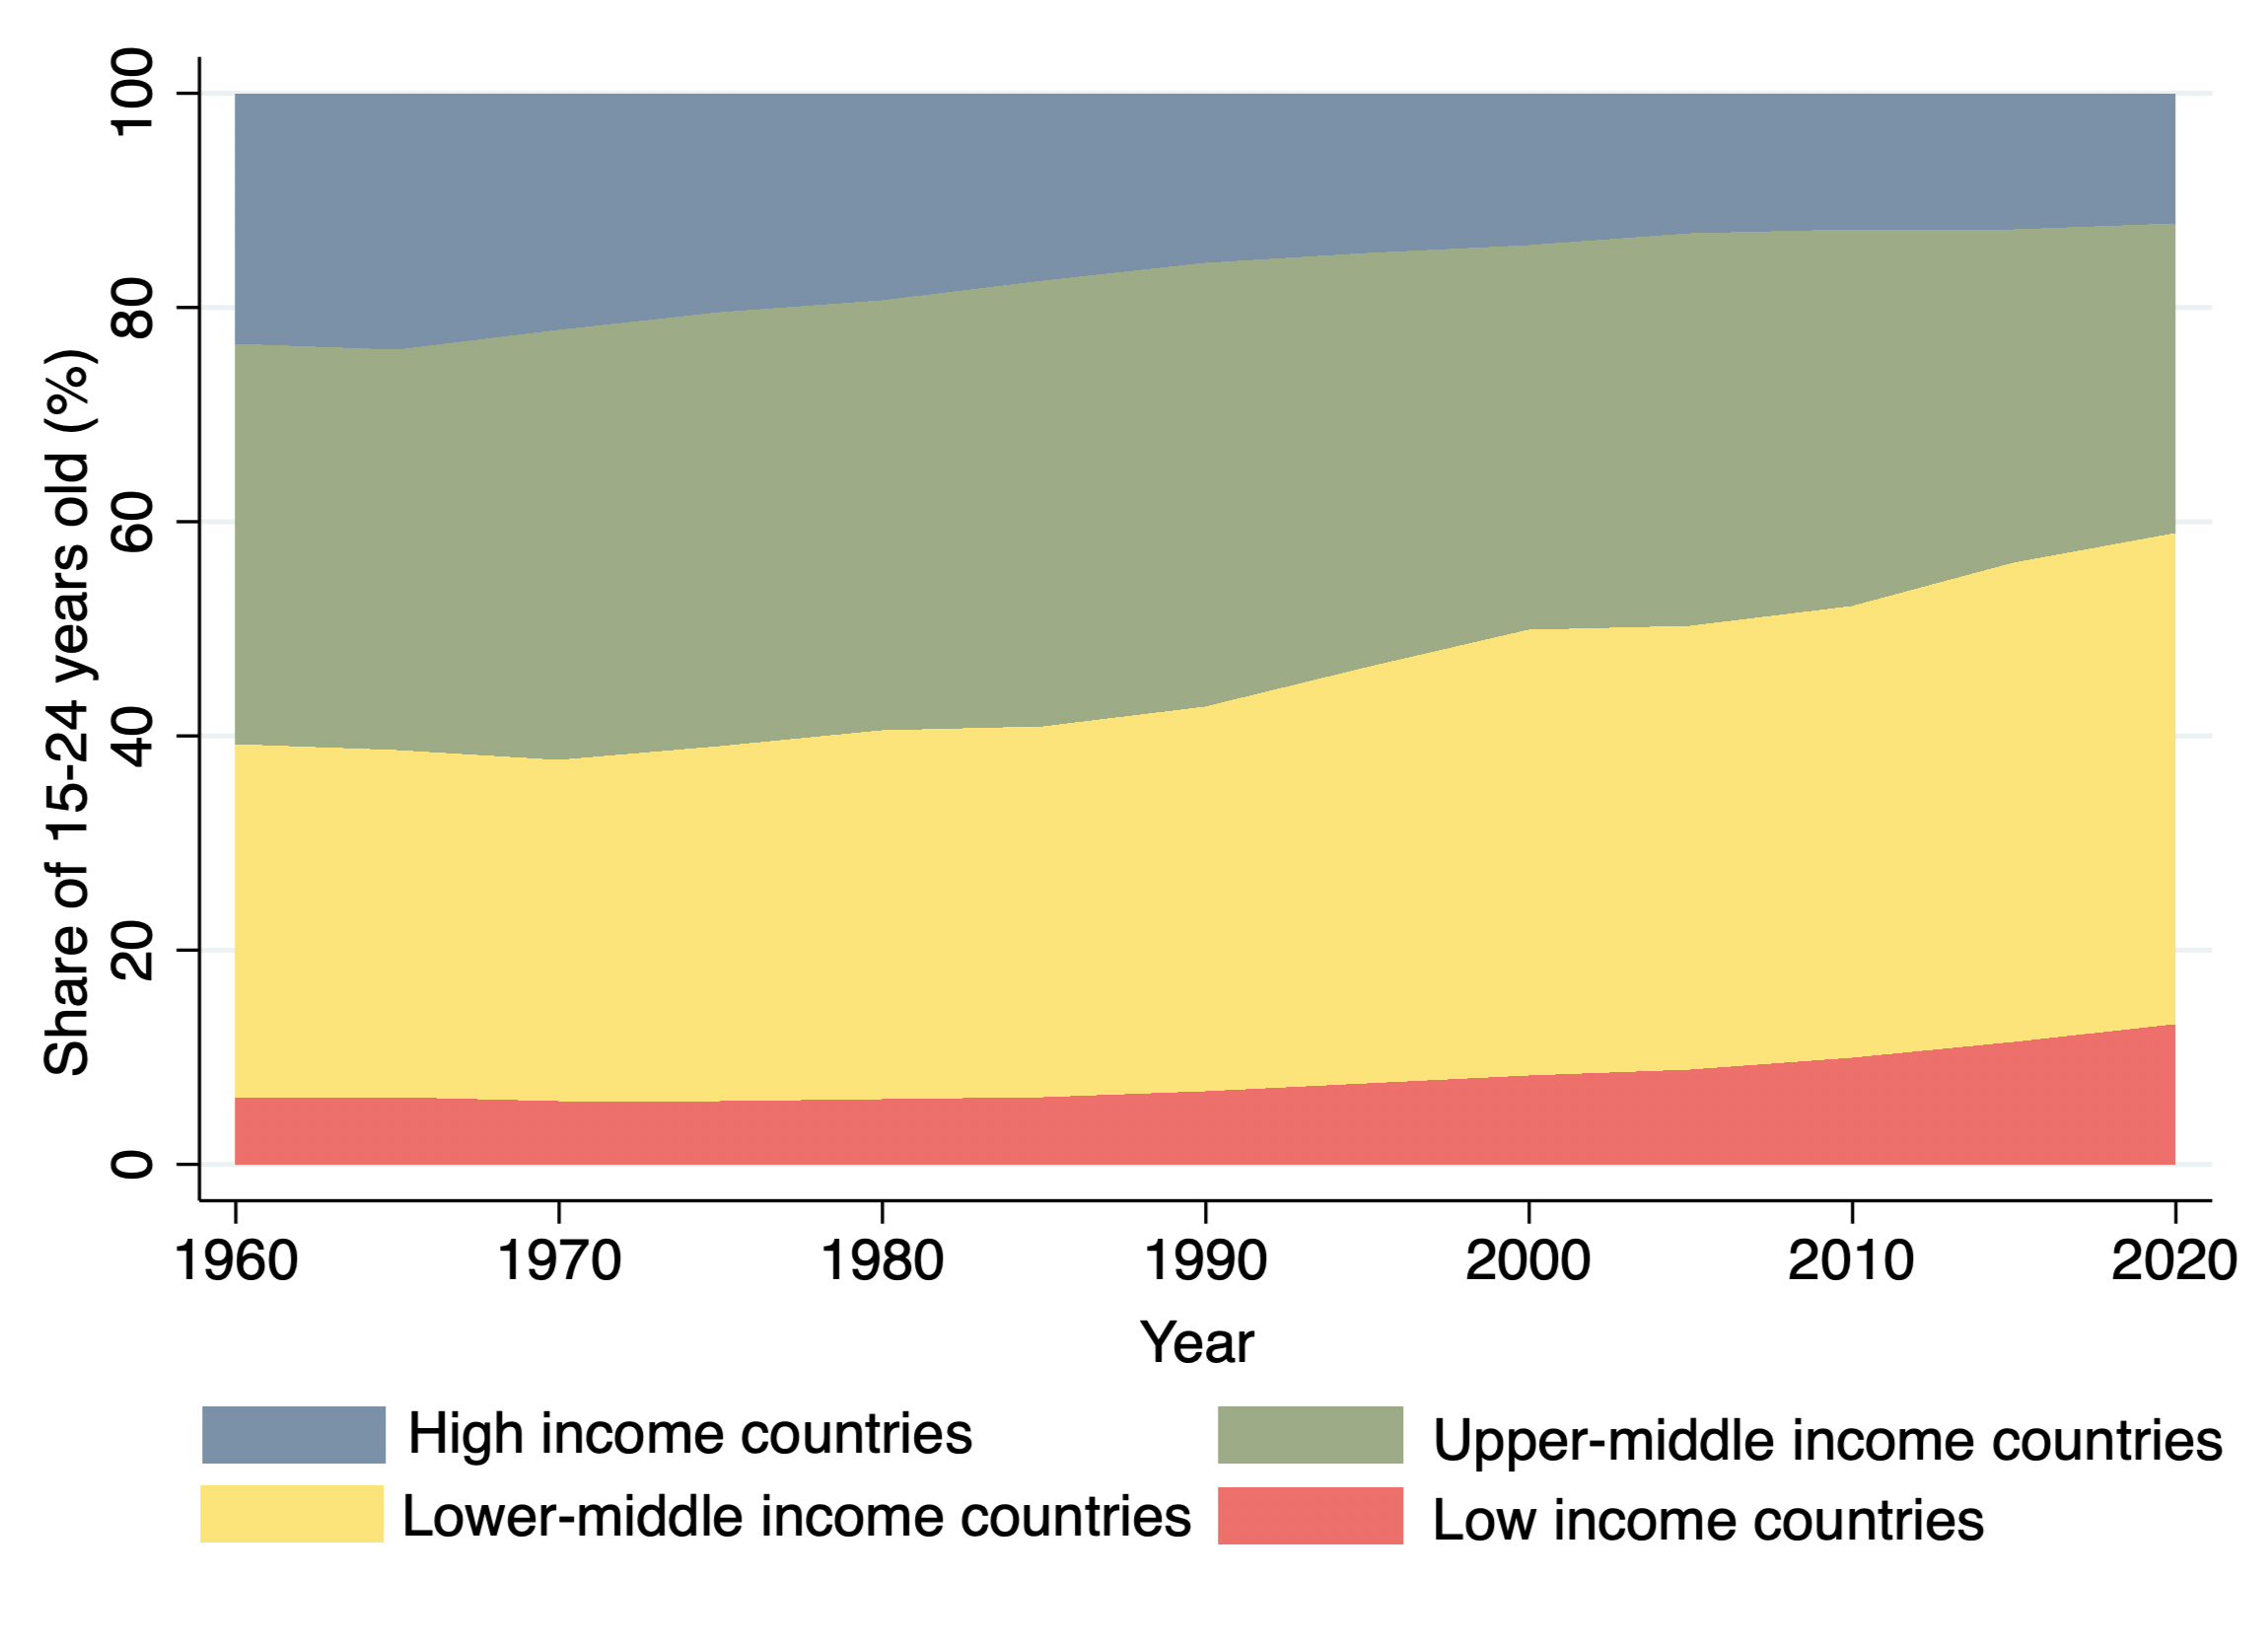
\includegraphics[width=0.49\linewidth,]{figures/relative_population} 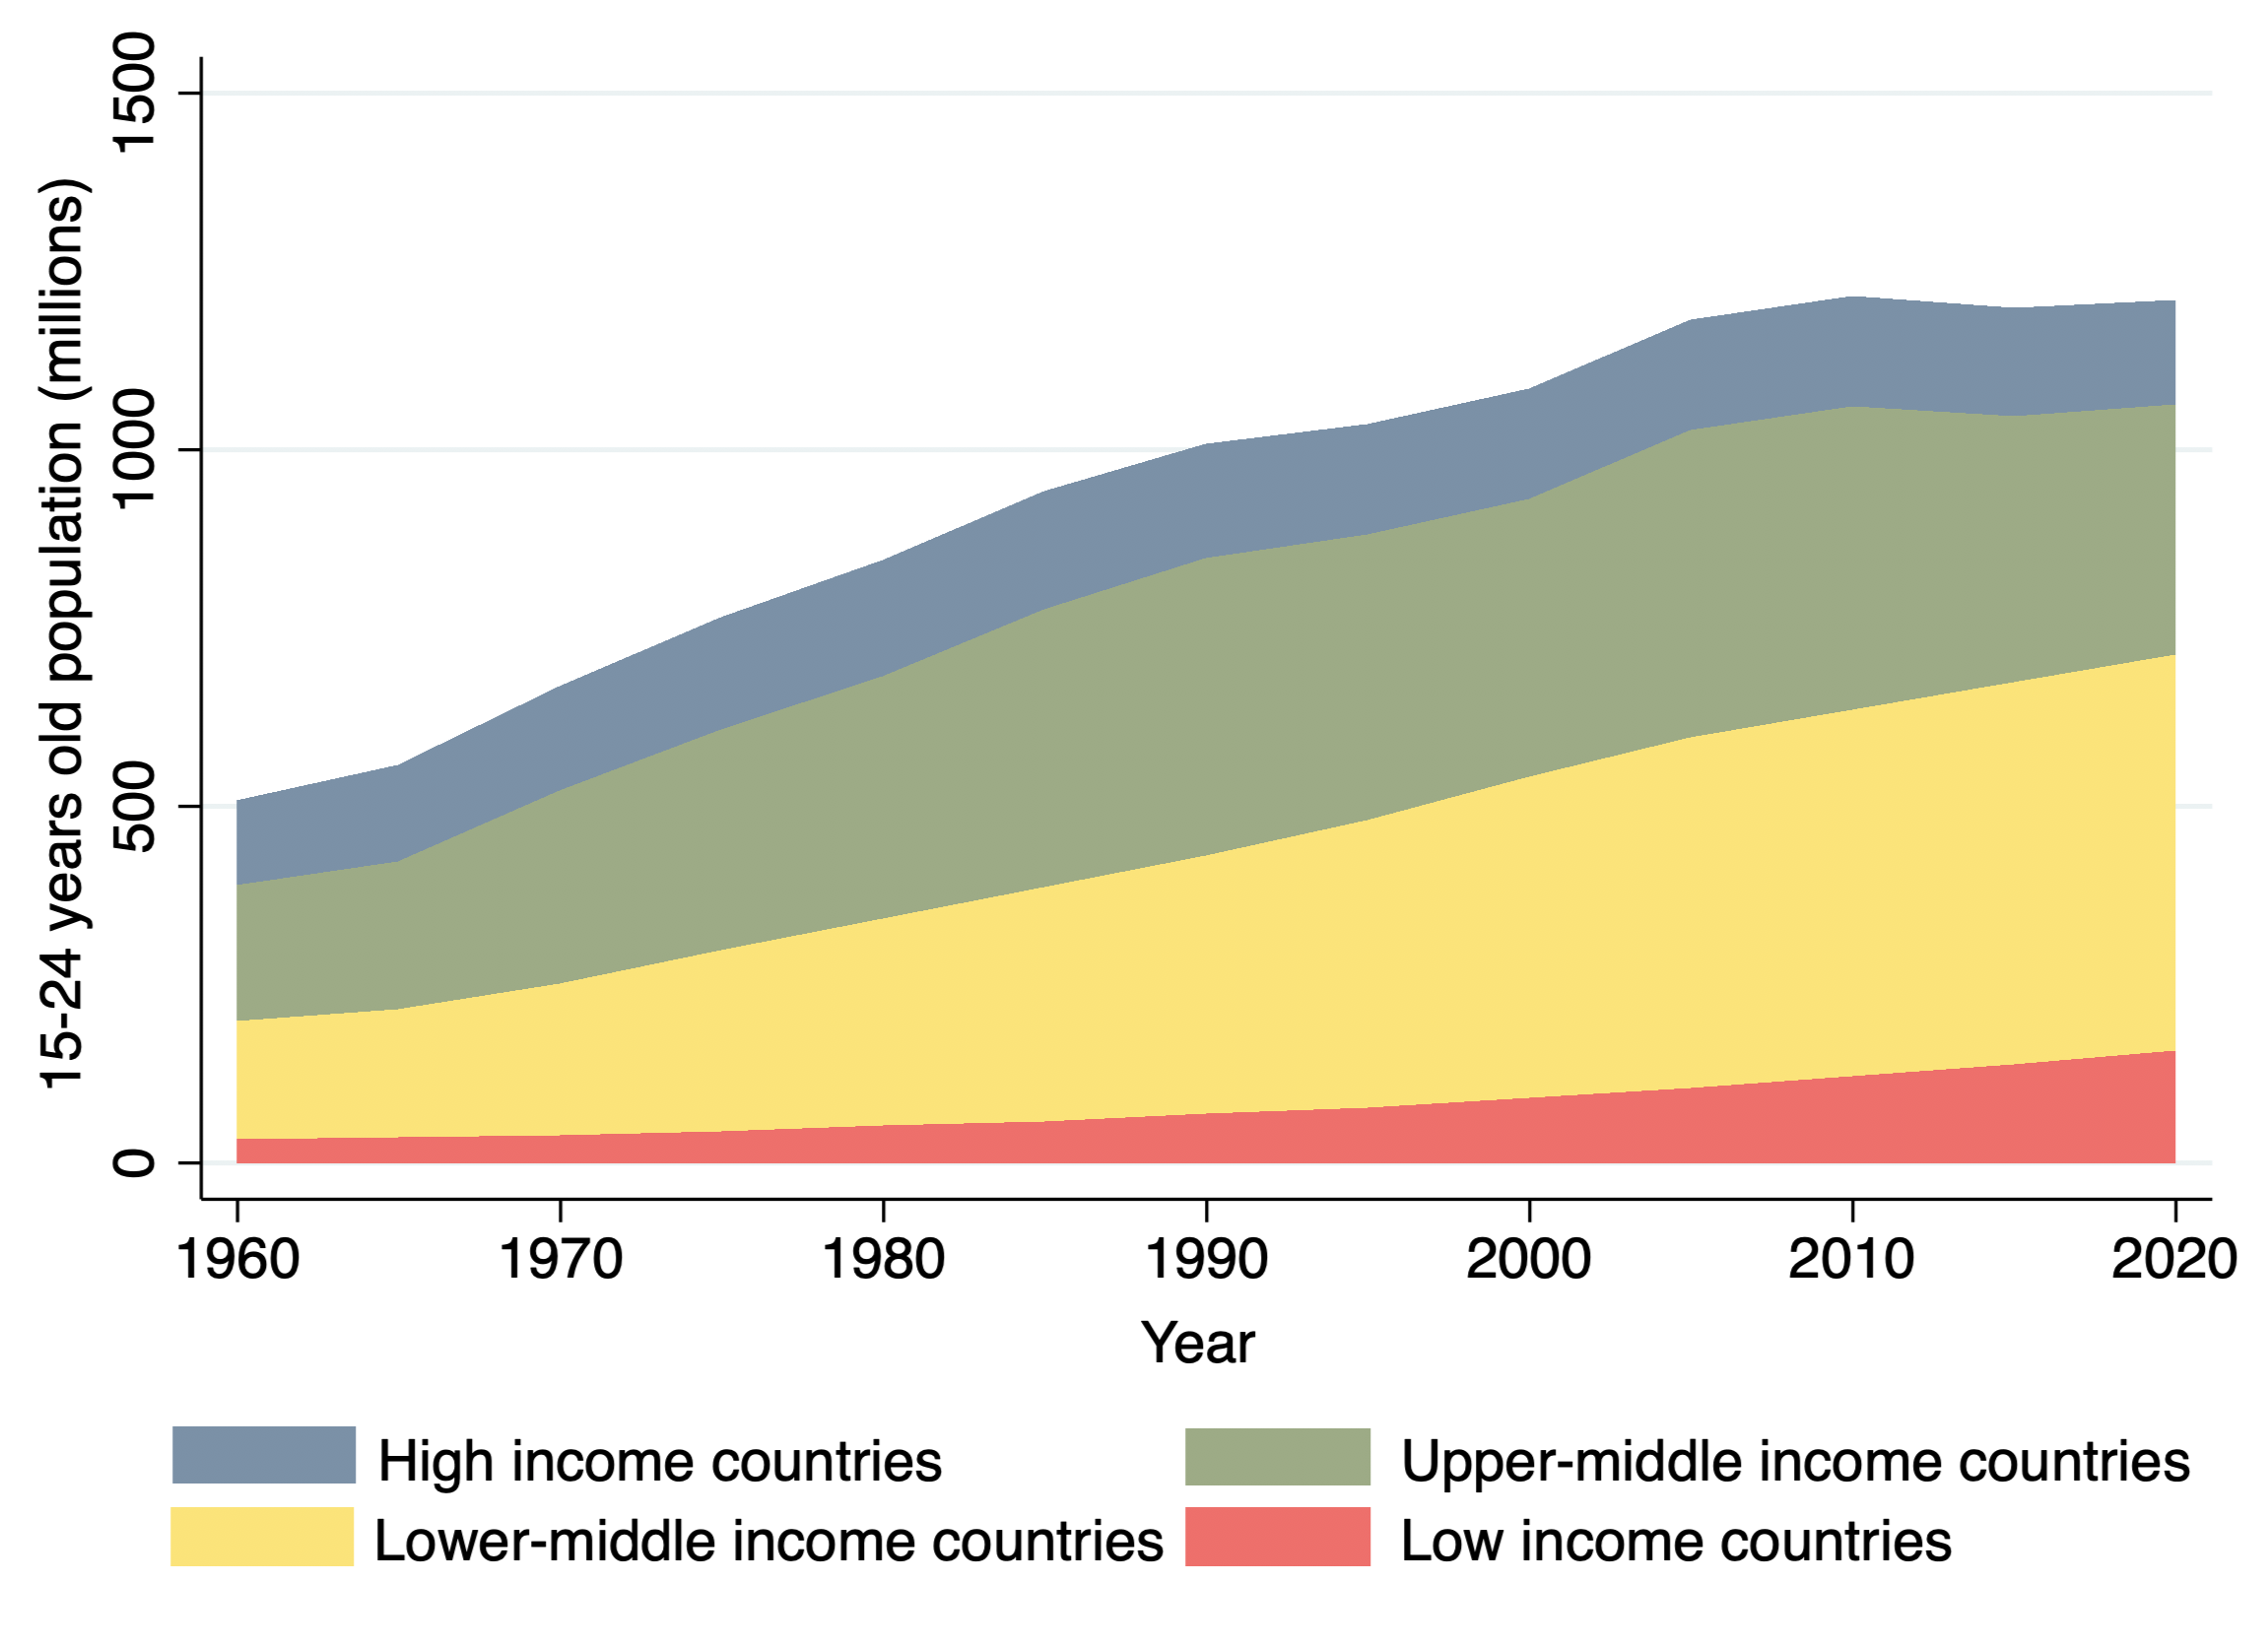
\includegraphics[width=0.49\linewidth,]{figures/total_population} 

}

\caption[World youth population, 1960-2020]{World youth population, 1960-2020 \\ \textit{\footnotesize{Source: World Population Prospects, United Nations (2019)}}}\label{fig:fig-youthpop}
\end{figure}

This ``youth bulge'' has implications for youth labor markets in SSA, where YLILI scores are among the lowest. On one hand, the population boom is an opportunity for growth. It has coincided with strong economic expansion in sub-Saharan Africa, with gross GDP growing an average of 4.35\% per annum between 2000 and 2019, compared to 1.75\% in the 20 years prior, per the World Bank. Experience from East Asia suggests that expanding working-age populations can contribute to economic transformation and rapid growth \autocite{bloom1998}, boosting demand for youth labor and improving their working conditions. On the other hand, the potential for a demographic dividend in SSA is curtailed by persistently low labor productivity and savings. Moreover, high dependency ratios prevent workers from being able to save and invest, and high fertility rates keep young women confined to the home, reducing the effective size of the labor force \autocite{eastwood2011}.

\begin{singlespace}

\begin{table}[H] \centering 
  \caption{Macro correlates, gender-specific YLILI and YLILI dimensions} 
  \label{tab:tbl-regwide} 
\footnotesize 
\begin{tabular}{@{\extracolsep{-8pt}}lcccccc} 
\\[-1.8ex]\hline 
\hline \\[-1.8ex] 
 & \multicolumn{6}{c}{\textit{Dependent variable:}} \\ 
\cline{2-7} 
\\[-1.8ex] &  & \textit{\underline{YLILI score}} &  &  & \textit{\underline{Dimension}} &  \\ 
 & Overall & Male & Female & Transition & Work. cond. & Education \\ 
\hline \\[-1.8ex] 
 log GDP & $-$1.711 & $-$0.609 & $-$1.711 & $-$5.961 & 6.123$^{***}$ & $-$3.183 \\ 
  & (1.814) & (1.221) & (1.814) & (4.420) & (2.237) & (2.619) \\ 
  & & & & & & \\ 
 Youth pop. ratio ($\times$ 100) & $-$0.697 & $-$1.199$^{***}$ & $-$0.697 & $-$0.199 & $-$0.834 & $-$1.364$^{**}$ \\ 
  & (0.465) & (0.290) & (0.465) & (1.118) & (0.502) & (0.618) \\ 
  & & & & & & \\ 
 Fertility rate & $-$4.271$^{***}$ & $-$2.278$^{***}$ & $-$4.271$^{***}$ & $-$3.827$^{*}$ & $-$2.129$^{*}$ & $-$6.987$^{***}$ \\ 
  & (0.868) & (0.607) & (0.868) & (2.114) & (1.096) & (1.266) \\ 
  & & & & & & \\ 
 Agriculture (\% of GDP) & $-$0.201$^{*}$ & $-$0.135$^{*}$ & $-$0.201$^{*}$ & 0.220 & 0.051 & $-$0.591$^{***}$ \\ 
  & (0.116) & (0.080) & (0.116) & (0.274) & (0.147) & (0.157) \\ 
  & & & & & & \\ 
 Manufacturing (\% of GDP) & $-$0.071 & $-$0.161 & $-$0.071 & 0.278 & $-$0.021 & 0.031 \\ 
  & (0.181) & (0.121) & (0.181) & (0.432) & (0.198) & (0.261) \\ 
  & & & & & & \\ 
 Exports (\% of GDP) & 0.069 & $-$0.006 & 0.069 & 0.084 & 0.028 & $-$0.037 \\ 
  & (0.057) & (0.038) & (0.057) & (0.138) & (0.070) & (0.078) \\ 
  & & & & & & \\ 
\hline \\[-1.8ex] 
Observations & 47 & 47 & 47 & 51 & 54 & 56 \\ 
R$^{2}$ & 0.661 & 0.682 & 0.661 & 0.127 & 0.574 & 0.730 \\ 
\hline 
\hline \\[-1.8ex] 
\multicolumn{7}{l}{$^{*}$p$<$0.1; $^{**}$p$<$0.05; $^{***}$p$<$0.01} \\ 
\multicolumn{7}{l}{\textit{Notes:} Standard errors shown in parentheses. YLILI score is on a scale of 0-100.} \\ 
\end{tabular} 
\end{table} 
\end{singlespace}

While the impact of population growth on a specific labor market will depend on idiosyncratic factors such as industrial composition, informal sector size, government policy, and the country-specific elasticity of labor demand, we can still use the YLILI to provide some evidence about the broader demographic determinants of the cross-country differences in youth labor market conditions. Columns (4) and (5) of Table \ref{tab:tbl-regwide} present the relationship between two demographic indicators and the YLILI score. The first, the youth population ratio, is defined as the population aged 15--24 divided by the total population. This ratio ranges from 0.095 to 0.223 for LICs and LMICs, with a mean of 0.189. It has been slowly increasing for low-income countries over the past 2 decades (from 19.5 percent in 2000 to 20.2 in 2020) and decreasing for lower-middle income countries (from 19.7 percent in 2000 to 17.9 percent in 2020). The youth population ratio is negatively correlated with the YLILI score: a one percent increase in the youth ratio is associated with a 2 point decrease on the YLILI scale. The fertility rate per country, which measures the number of births per woman and ranges from 1.262 to 6.913 and a mean of 3.72, exhibits an even stronger relationship: an additional birth per woman---slightly less than one standard deviation---is associated with a 4.6 point decrease in the YLILI score. When these two demographic variables are regressed together with GDP per capita on the YLILI score (column 6), income is no longer a statistically significant predictor of the YLILI score. In other words, the size of the youth bulge appears affect youth labor market strength, even among among countries at similar levels of economic development. This can also be seen in Figure \ref{fig:fig-indexgdp} in the Appendix: several countries with middling income levels---e.g., Haiti, Nepal, Kyrgyzstan, and Cambodia---are still able to offer their youth relatively attractive labor conditions.

Columns (7) and (8) attempt to discern whether the structural features of an economy are able to explain differences in youth labor market performance. In model (7), we retain GDP per capita, the youth ratio, and the fertility rate, and introduce three measures of the structural composition of the economy: share of GDP in agricultural production, manufacturing, and export volume, respectively. In model (8), GDP is dropped in favor of more detailed indicators such as foreign direct investment (FDI), the national savings rate, urbanization and electrification rates, and the Ease of Doing Business index score \autocite[from the][]{worldbank2021a}. In both specifications, the two demographic variables remain highly significant at conventional levels. When controlling for income levels and demographics, more agrarian economies are found to have weaker youth labor markets. This is consistent with youth leaving work in agriculture \emph{en masse} and characterizations of agricultural work as relatively low-productivity and low-income \autocite{filmer2014}. Foreign direct investment, on the other hand, is associated with better employment outcomes for youth.

We repeat this analysis for the gender-disaggregated rankings of the YLILI and the three dimensions of the overall (not gender-specific) YLILI using the preferred specification in column (7). The results are shown in Table \ref{tab:tbl-regwide}. While higher youth ratios are associated with worse labor market outcomes for males, high fertility rates have a much stronger negative impact on females. In other words, high fertility rates decrease labor force participation and other labor market outcomes for young women in the present \autocite[in line with][]{bloom2009}, while reducing labor market prospects for young men in the future.

\todo{6} \hlc[pink]{Table }\ref{tab:tbl-regwide} \hlc[pink]{also shows that different dimensions of the YLILI correlate with different macroeconomic measures. A high fertility rate, for instance, is associated with lower transition scores, likely reflecting its the detrimental effects of childbirth on female economic participation. On the other hand, richer countries experience slower youth transitions to the labor market---again, because extended periods of inactivity after leaving school is a luxury that youth in lower-income countries cannot afford. In contrast to the overall YLILI score, the working conditions dimension score is predicted by GDP per capita, even after controlling for demographic variables. Thus, even if economic growth is not a solution to all aspects of the youth employment problem, it can still lead to short-term improvements by alleviating youth working poverty, underemployment, and work informality. Finally, education outcomes are shown to be worse for countries with higher youth ratios (possibly via overburdened education systems) and fertility rates (higher dropout rates for females).}

\hypertarget{the-gender-ylili}{%
\subsection{The gender YLILI}\label{the-gender-ylili}}

All of the component indicators of the YLILI are disaggregated by gender, allowing us to make cross-country comparisons of male- and female-specific YLILI scores, as well as analyze YLILI gender gaps within and between countries.

Encouraging gains have been made in female access to education, literacy, and maternal mortality in the past two decades, though progress on labor market equality has been slower. Labor force participation rates in particular remain much lower for women than men in most developing countries. Regional levels of female labor force participation (FLFP) are heterogeneous and are not predicted by GDP, female education, or fertility \autocite{klasen2019}. FLFP is relatively low in Southern Asia and MENA, for instance, despite rapid declines in fertility and expanding female access to education and relatively high in both Eastern Europe and Central and East Asia. FLFP is also high in SSA, despite relatively low female education attainment, low incomes, and high fertility rates in the region. In fact, while youth labor force participation is decreasing---most of the world, it is increasing for young women in SSA---albeit from a low baseline \autocite{ilo2023b}.

Other gender inequalities remain pronounced in parts of the developing world. Reliable data on the gender wage gap in low-income countries is scarce, but limited evidence also shows significant variation, from 20 percent in Mozambique and Pakistan to more than 80 percent in the Ivory Coast \autocite{worldbank2011}. A recent study shows that as countries get richer, women tend to concentrate into an ever smaller number of occupations (even as they branch out into new sectors) ---thus perpetuating gender segregation in the workplace \autocite{borrowman2020}. Women in low-income countries work in the informal sector at higher rates than men: they are less likely to be an employer, own land, or have control over their finances, particularly in SSA and Southern Asia \autocite{ortiz-ospina2018}, and up to three times more likely to be a contributing family worker \autocite{bonnet2018}. Such gender-based labor market inequalities start young and can hamper prospects for growth in the long term \autocite{undp2019}.

Average dimension and indicator scores for the gender-specific YLILI are presented in Table \ref{tab:tbl-gender} in the Appendix. Labor market conditions in LICs and LMICs favor young men by an average of just under 3 points on the YLILI scale. There is a negative and marginally significant correlation between the gender difference in YLILI score and the aggregated YLILI itself: countries in which women are most disadvantaged are Afghanistan (ranked 51st out of 54 overall on the YLILI), India (14th), Senegal (36th), and Pakistan (34th), while the Philippines (10th overall), Lesotho (20th), Nicaragua (16th), Honduras (25th) and Ghana (28thst) are among the countries with a higher female than male YLILI (see Tables \ref{tab:tbl-gendiff} and \ref{tab:tbl-gendiffdims} in Appendix B2 for country-by-country performance and Figure \ref{fig:fig-gendercorr} for a visual representation). We find no relationship between the national gender gap and GDP per capita.

The dimension scores for male and females are shown across the top panel of Figure \ref{fig:fig-gendercorr}. The gender differences are largest on the transition dimension, with a mean transition score of 82.3 for men and 75.56 for women. The gender gap in transition scores is driven primarily by high inactivity among young women: the average NEET rate for female youth in our sample is 33.5 percent, compared to 17.7 percent for males--- significantly higher than the global gap (31.1 percent for females versus 13.9 percent for males \autocite{ilo2023b}). Developing countries with the most exacerbated gender differences in the NEET rate are Afghanistan, Yemen, Pakistan, Bangladesh, and India, suggesting that regional cultural attitudes play an important role in determining female labor market participation.

\begin{figure}[H]

{\centering 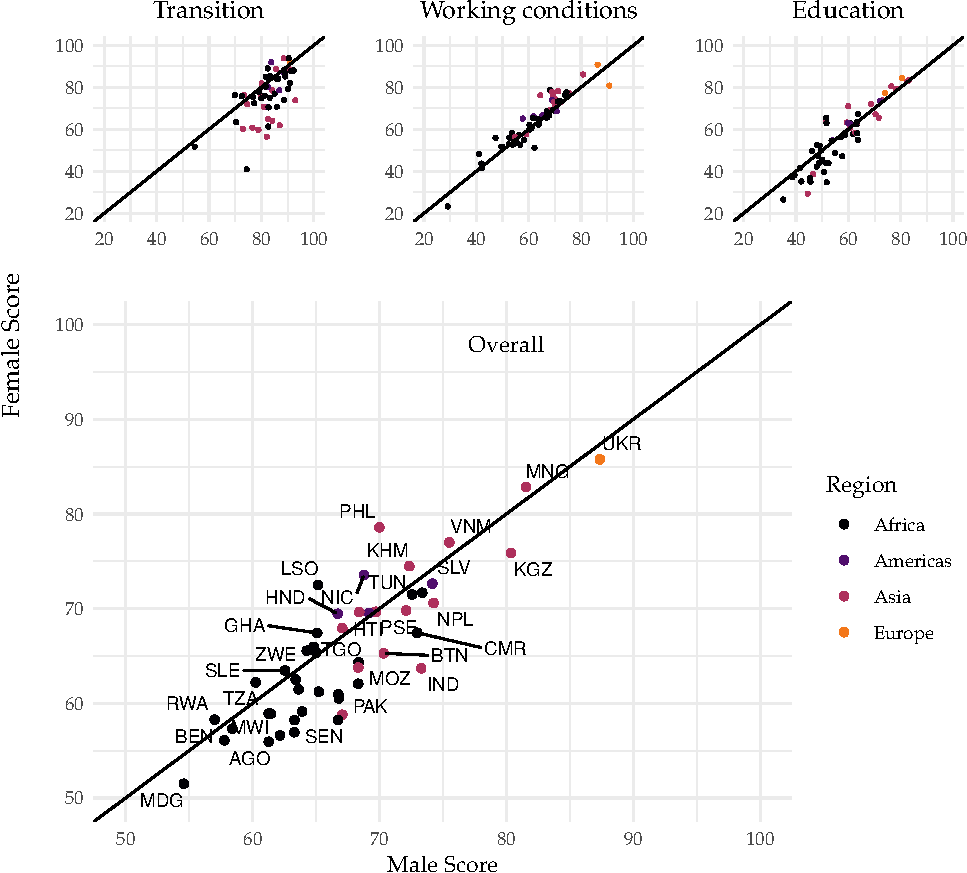
\includegraphics{figures/fig-gendercorr-1} 

}

\caption{YLILI score by gender}\label{fig:fig-gendercorr}
\end{figure}

Conditional upon entering the labor market, young women appear to enjoy a higher quality of work than young men, scoring 0.74 points higher on the working conditions dimension. Countries at the top of the YLILI rankings in particular have lower rates of female informal and elementary work (Table \ref{tab:tbl-gendiffdims} in Appendix B2). However, these rates only pertain to youth participating in the labor market, and thus neglect the substantial numbers of women working as caregivers or unpaid household laborers \autocite{ilo2023b}, who are reflected instead in higher NEET rates for women.

Finally, while countries in our sample appear to have only a minor gender imbalance in the education dimension---1.86 points higher for males---there is significant underlying variation between countries and within individual indicators. Women outperform men on harmonized test scores on average, with high female performance in the Occupied Palestinian Territory, Egypt, the Sudan, Moldova, and Algeria. However, they perform poorly in test scores and literacy rates. Young women face substantial education deficits in countries that perform poorly on the YLILI overall, with Niger, Afghanistan, Chad, Angola, and Benin being among the worst performers in terms of both literacy and secondary school attainment.

To investigate a possible determinant of these gender differences in youth labor markets, we examine the relationship between the YLILI gender gap and the Council on Foreign Relations Women's Workplace Equality Index (which is measured on a scale from 0 to 100 and is based on seven indicators: accessing institutions, building credit, getting a job, going to court, protecting women from violence, providing incentives to work, and using property). We observe a strong positive linear correlation (0.33, significant at p \textless{} 0.001) between the female YLILI and the CFR Index and a strong negative correlation (-0.156, significant at p \textless{} 0.0001) between the YLILI gender gap and the CFR Index, suggesting that institutional and legal protections for women in the workplace can help reduce gender inequalities in youth labor markets.

\hypertarget{robustness}{%
\section{Robustness}\label{robustness}}

An important consideration when evaluating the usefulness of the YLILI is its sensitivity to the choice of indicators and aggregation methods used in its construction. Though data availability was the main determinant of which indicators were included, the methodological choices described in Section \ref{methods} still leave many degrees of freedom. Regardless of the final combination of indicators, the index should be robust to the inclusion or exclusion of any particular variable, as well to choices regarding the number of included variables, the way they are aggregated, and the choice of whether and how to impute missing observations. To test the robustness of the YLILI, we observe the changes in scores and rankings when different specifications are used.

Five measures are summarized in Table \ref{tab:tbl-altspecs}. For index scores, we report the correlation between the scores generated by alternative index specifications and the original YLILI score, along with the standard deviation of their differences. For country rankings, we compute the Spearman correlation along with the mean and maximum rank differences between the original YLILI and proposed alternatives. We conduct these tests for 12 specifications: ten consisting of the same aggregation and imputation method, but dropping a single indicator (resulting in indices containing nine indicators). One specification was generated using the geometric mean to aggregate across indicators and dimensions, and one using raw data only (without imputation).

\begingroup
\renewcommand*{\arraystretch}{1.5}
\begin{table}[ht] \centering 
  \caption{Alternative specifications} 
  \label{tab:tbl-altspecs}
\begin{adjustwidth}{-.2cm}{}
  \scriptsize{
\begin{tabular}{rrrrrrrrrrrrr}
 \hline \hline \\[-1.8ex] 
 & \rot{no neet} & \rot{no relative wc} & \rot{no mismatch} & \rot{no workingpov} & \rot{no underemp} & \rot{no informal} & \rot{no elementary} & \rot{no nosecondary} & \rot{no literacy} & \rot{no test scores} & \rot{geometric} & \rot{raw} \\ 
  \hline \\[-1.8ex] 
Pearson's $r$ & 0.982 & 0.987 & 0.983 & 0.953 & 0.981 & 0.981 & 0.975 & 0.980 & 0.990 & 0.983 & 0.939 & 0.926 \\ 
%Mean score diff. & 1.272 & 1.524 & 1.150 & 2.108 & 1.315 & 5.889 & 1.202 & 1.325 & 4.652 & 5.190 & 12.439 & 1.785 \\ 
Std dev. of score diff. & 1.499 & 1.388 & 1.450 & 2.389 & 1.505 & 1.541 & 1.816 & 1.556 & 1.129 & 1.545 & 5.259 & 3.454 \\ 
Spearman's $\rho$ & 0.968 & 0.985 & 0.972 & 0.927 & 0.976 & 0.976 & 0.965 & 0.967 & 0.982 & 0.977 & 0.924 & 0.924 \\ 
Mean rank diff. & 2.704 & 1.926 & 2.704 & 4.333 & 2.481 & 2.370 & 2.852 & 2.926 & 2.185 & 2.296 & 4.741 & 3.926 \\ 
Max. rank diff. & 12  & 7  & 10  & 16  & 9  & 12  & 12  & 10  & 9  & 11  & 15  & 24 \\
  \hline \hline \\[-1.8ex] 
\end{tabular}
 \begin{tablenotes}
      \item \footnotesize \textit{Notes}: Correlations and differences relative to specification using 10 indicators, arithmetic mean, and imputed values.
    \end{tablenotes}
}
\end{adjustwidth}
\end{table}
\endgroup

\todo{2}\hlc[pink]{Scores and rankings for all countries were recalculated with the alternative specifications and are shown in Table} \ref{tab:tbl-altscores} \hlc[pink]{in Appendix B2. Scores and ranks remain highly correlated with the original YLILI when a single variable is dropped, indicating that the index is not overly dependent on the inclusion of any particular measure. Alternative specifications impact the countries in the middle of the index much more than those at the extremes. Neither score nor rank correlation drops below 0.9 for any of the alternative specifications studied. Removing the youth working poverty rate causes the largest overall changes in scores and reordering of rank, with countries changing rank by 4.3 positions on average.}

When the geometric rather than the arithmetic mean is used to aggregate both the indicators into dimensions and dimensions into the final YLILI score, rankings and scores when using the two indicator aggregation methods remain strongly correlated despite the significant shift in the absolute scores (Figure \ref{fig:fig-arithgeom} in Appendix B2). Certain scores and ranks change when data is not imputed, with India moving ranks by an entire 24 positions (from rank 14 with imputed data to rank 38 without), as depicted in Figure \ref{fig:fig-imputedraw} in Appendix B2. Given the conceptual justification for imputation, however, this is only reassuring that imputation is necessary for delivering consistent results.

As with any composite index, several caveats and limitations warrant discussion. In general, composite indices have faced increased scrutiny even as their popularity has increased in recent years. \todo{3}\hl{One of the most common critiques is subjective weighting: even minor adjustments in weight assignments can exert substantial influence on the resultant rankings.  While some authors use data-driven weights such as PCA }\autocite{becker2017}\hl{, such methods provide a weighting of components based solely on the variance of the data, without consideration for the underlying importance of each variable or component in explaining the phenomenon being measured. Moreover, even if one could derive the "objective" weighting of all indicators relevant for describing youth labor markets, the full set of indicators would almost certainly not be available due to data limitations in our context. Our solution is to rely on an imperfect, but transparent, equal weighting, while providing an online tool for experts to adjust the weights according to their understanding and experience..}

\todo{2}

\hl{A common consideration for composite indices is the concept of "multidimensionality": if each pair of component variables exhibits high correlation, then the index may not truly represent multiple dimensions, and a single dimension might suffice. However, we have shown that the three dimensions of the YLILI do not exhibit high correlation, at least during the time period under consideration, and substituting a single dimension for the YLILI would result in substantial information loss and and a different ranking.}

\todo{2}

\hl{Another question that often arises is whether the composite index could be reduced to a smaller number of indicators. If a smaller number of components can essentially provide the same ranking as the full composite index, it may seem more logical to utilize the former rather than the latter. However, though indicators within dimensions do exhibit a degree of correlation, they were chosen to be conceptually distinct, such that a smaller number of indicators would inadequately reflect the diversity of factors within that dimension. Moreover, as argued by} \autocite{foster2013}\hl{, it is crucial to maintain a balance between ensuring statistical association among indicators and avoiding excessive redundancy, as removing correlated indicators may compromise the robustness of the index.}

A common critique, leveled at the HDI in particular, concerns the implicit trade-offs resulting from the aggregation of indicators: in the HDI, the inclusion life expectancy and GNI implies a value of an additional year of life in terms of economic output, for instance \autocite{ravallion2012}. None of the 45 indicator pairs in the YLILI imply ``shadow prices'' this problematic, though the youth working poverty indicator could be juxtaposed with less ``economic'' components of the YLILI, such as the literacy rate, in order to level a criticism along similar lines.

While a historical YLILI time series would have been ideal for studying policy impacts and changes in youth labor markets over time, the infrequency and scarcity of retrospective data ultimately proved to be insurmountable. Although labor market statistics for LMICs and LICs have become more frequent and reliable in recent years, administrative data quality in some countries remains so poor that two SDG subgoals were aimed at data collection capacity. For instance, the NEET rate, the primary indicator for tracking progress on youth employment for SDG 8, was last collected in 2005 in Congo and 2002 in Guinea, and it is not available on the ILO database at all for several lower-middle income countries, including Morocco and Tajikistan. With improved data coverage, future editions of the YLILI may be able to provide insights about changes in youth labor market strength over time.

\hypertarget{discussion}{%
\section{Discussion}\label{discussion}}

In the decades to come, youth working populations are expected to boom in many low-income and lower-middle income countries. Providing opportunities for decent and gainful work for youth while facing the dual headwinds of persistent informality and slow structural change will be a key challenge for policymakers. The Youth Labor Index for Low-Income Countries offers a holistic, quantitative picture of LIC and LMIC youth labor market strength, with an explicit focus on the quality of work for youth, to help measure progress on this development goal and to provide guidance for policy decisions.

Despite data limitations, we are able to generate the YLILI for 54 out of 79 LMICs and LICs. Countries in SSA represents the bulk of the sample, and generally perform poorly on the YLILI compared to the rest of the developing world. Scores in SSA are particularly low for working poverty, education quality, and secondary school completion. Transition smoothness, as measured by rates of inactivity, differences in working conditions for youth and adults, and job mismatch, are fairly homogeneous for the entire sample, while important variation exists across countries for both working conditions and education scores. The high variation in education outcomes in particular drives the final ordering of the YLILI rankings. Gender differences are most apparent in the transition dimension, with low female labor force participation, particularly in Southern Asia, standing as a major obstacle to achieving labor market equality in the developing world. The YLILI gender gap is negatively correlated with the CFR Workplace Equality Index, suggesting that institutional and legal protections for women in the workplace are important tools that may help reduce gender inequalities in youth labor markets.

Our most striking finding is the degree to which the YLILI score is predicted by demographic patterns, specifically the ratio of youth to adults in the working population and the fertility rate. Countries with very young populations score considerably worse on the YLILI, especially when only data for males is used. Meanwhile, income is not predictive of youth labor market strength once demographic characteristics are accounted for, suggesting that population growth puts youth labor markets under pressures that cannot simply be alleviated through higher economic growth. Higher youth population ratios are associated with worse education outcomes, signaling that rapidly growing populations are stretching the capacities of their education systems to a breaking point. However, among the macroeconomic determinants considered, fertility rates are the best predictor of YLILI scores, particularly for women. The birth of a child has been shown to shorten the working lives of women by as much as two years on average \autocite{bloom2009}. We find that this negative impact extends to youth labor markets as a whole: an additional birth per female at the national level is associated with a 4.6 point decrease in the (overall) YLILI score, or about 0.6 of a standard deviation. The likely channels are decreases in economic activity and educational attainment resulting from childbearing, both of which factor into the YLILI.

Existing indices similar to the YLILI in construction have aimed to capture youth quality-of-life more generally. The Youth Development Index combines 18 measures of youth education, health and well-being, employment opportunity, and political and civic participation to rank 183 countries \autocite{sen2016}. The Youth Progress Index combines 60 indicators to measure a similar concept, but explicitly excludes economic variables to allow for comparisons with GDP \autocite{lisney2018}. Both indices suggest that youth well-being is very tightly correlated with per-capita income, especially at lower income ranges, but they do not share our explicit focus on labor market outcomes. In contrast, we only find a weak correlation between per-capita GDP and youth labor market strength: for instance, the fourth-ranked country on the YLILI score, Kyrgyzstan, has the same GDP per capita as the 46th-ranked country, the Ivory Coast. When controlling for demographic characteristics, income is only correlated with youth working conditions, but not the YLILI index score itself.

How can the YLILI help policymakers improve youth labor markets in developing countries? First, the global score gives a sense of how far the country is from the ideal state (=100). It also gives a sense of the relative position of the country compared to other LICs and LMIcs. Second, the breakdown of the index into ten indicators and three dimensions allows users to identify the most pressing issues facing a given economy. For instance, the index suggests that Pakistan should focus on improving education, on which it scores 30 points lower than on the other two dimensions. In contrast, Zimbabwe should focus on enhancing its working conditions: nearly half of its working youth are employed in elementary occupations, placing it in the bottom 7 percent of developing countries. Finally, the fact that the index is age- and gender-specific allows policymakers to obtain insights for targeted groups of the population. The accompanying \href{https://nadel.shinyapps.io/ylili}{webtool} is designed to facilitate this process by allowing users visualize the index, download the underlying data, and directly compare countries along the various index components.

Finally, the YLILI shows the usefulness of detailed, gender-disaggregated data, and could still be vastly improved with more comprehensive national statistics. The fact that we were unable to generate a score for 25 countries---almost a third of the sample----despite relatively relaxed requirements (e.g., including data up to a decade old), highlights the data scarcity which makes the study of youth labor markets a challenge \autocite{jerven2013}. We note that even major compilers of international statistics such as \href{https://ourworldindata.org/}{Our World in Data}, which have conducted numerous detailed analyses of topics related to the SDGs, do not have a page dedicated to the youth employment crisis at this time. Improving statistical capacity would thus be a major step towards an improved YLILI and towards more effective policies addressing the youth employment challenge.

\newpage
\markboth{References}{References}
\printbibliography[segment=\therefsegment,heading=subbibintoc,title={References}]

\newpage

\hypertarget{appendix-a}{%
\section*{Appendix A2}\label{appendix-a}}
\addcontentsline{toc}{section}{Appendix A2}

\markboth{Appendix A2}{Appendix A2}

\setcounter{figure}{0}
\renewcommand{\thefigure}{A2.\arabic{figure}}
\setcounter{table}{0}
\renewcommand{\thetable}{A2.\arabic{table}}

\todo{4}
\begin{figure}[H]
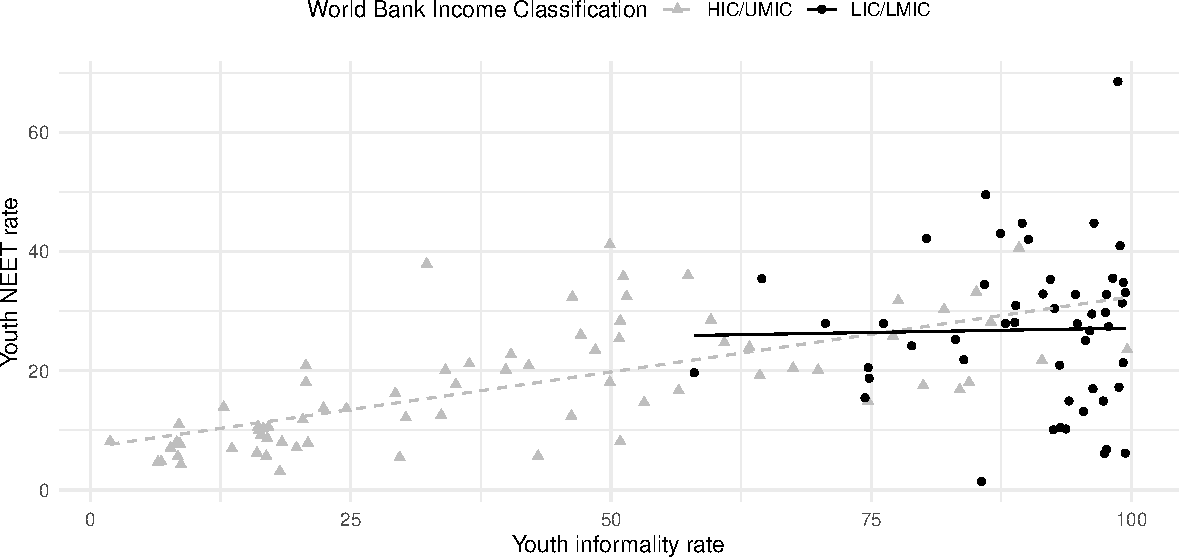
\includegraphics{figures/fig-infneet-1} \caption{Relationship between youth NEET rate and informality by income level}\label{fig:fig-infneet}
\end{figure}

\hypertarget{weights}{%
\subsection*{Index Construction}\label{weights}}

\markboth{Index Construction}{Appendix A2}

The working conditions ratio and harmonized test scores indicators are converted into a unit-less ``progress score'' ranging from 0 to 100 using the standard Min-Max method as follows:
\[ s_{idc}= \Bigl(\frac{\text{value}_{idc}- \text{min}_{id}}{ \text{max}_{id} - \text{min}_{id}} \Bigl) \cdot 100 \]
\vspace*{5pt}
where \(s_{idc}\) represents country \(c\)'s score for indicator \(i\)---which ranges from 0 to 100---for indicator \(i\) from dimension \(d\). \(\text{value}_{idc}\) denotes country \(c\)'s observed value for indicator \(i\). \(\text{min}_{id}\) is the value of indicator \(i\) at, or below which the score is 0. \(\text{max}_{id}\) is the value at, or above which the score is 100.

The challenge is to determine the value of both variables \(\text{min}_{id}\) and \(\text{max}_{id}\). Depending on the indicator, this could be a policy target, the theoretical max/min value, the most practical max/min value from a scaling perspective, a number derived from statistical analysis of the distribution, etc. Difficulties arise when the indicator is not naturally bounded, as in the case of the relative working conditions ratio (and thus of both ratios that construct it, i.e.~the working poverty ratio and the time-related underemployment ratio). As described in the text, the working conditions ratio is given higher and lower bounds of 10 and 1, while for the harmonized test score the natural bounds of 300 and 625 (the lowest and highest possible scores, respectively) are used.

A further design choice concerns the method of aggregation across indicators and dimensions. In most applications, this is either additive, such that individual components are summed to form the aggregate, or multiplicative, in which case it becomes the product of the parts. If indicators are rescaled before aggregation, the analogs of these two approaches become the arithmetic and the geometric mean, respectively. The current HDI uses both: in taking the average of two measures of school attainment, it uses the arithmetic mean at the dimension level, but takes the geometric mean of the three dimensions to arrive at the index score.

Geometric means are more appropriate for comparing items measured on different scales. The majority of the YLILI indicators are on the natural 0-100 percentage scale, but vary somewhat in distribution. It has also been suggested that multiplicative aggregation is more appropriate when good performance on all component dimensions is required simultaneously for a high aggregate score \autocite{sagar1998}, i.e., a country cannot score reasonably well while completely failing in a particular dimension. When using arithmetic means, changes in components enters the aggregate in absolute terms. For example, an increase from 1\% to 2\% in a given indicator would increase the aggregate by 1\% times the weight of the indicator. If using the geometric mean, on the other, the change in the aggregate would reflect the relative change in the indicator---100\% times its weight. A comparison of the two methods reveals close agreement in the final index scores (see Section \ref{robustness}); we refer to the score generated using the arithmetic mean in this paper due to its easier intuitive interpretation.

\hypertarget{correlations}{%
\subsection*{Index Correlations}\label{correlations}}

\markboth{Index Correlations}{Appendix A2}

\begin{figure}[H]

{\centering 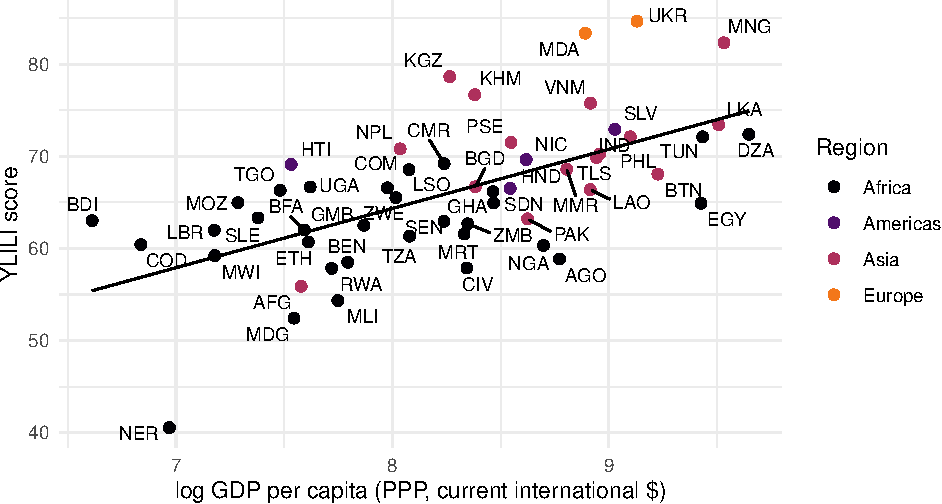
\includegraphics{figures/fig-indexgdp-1} 

}

\caption{Correlation, YLILI score and GDP per capita}\label{fig:fig-indexgdp}
\end{figure}

\begin{figure}[H]

{\centering 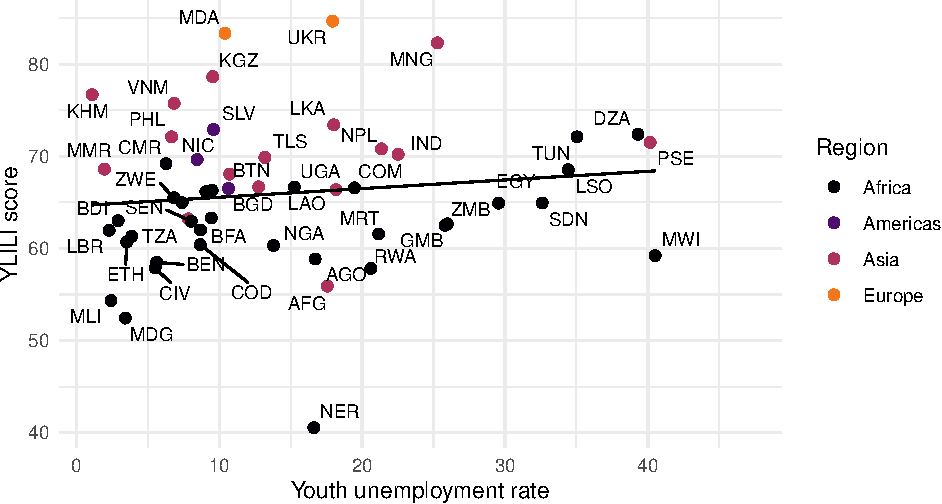
\includegraphics{figures/fig-indexunemp-1} 

}

\caption{Correlation, YLILI score and national youth unemployment rate}\label{fig:fig-indexunemp}
\end{figure}

\begin{figure}[H]

{\centering 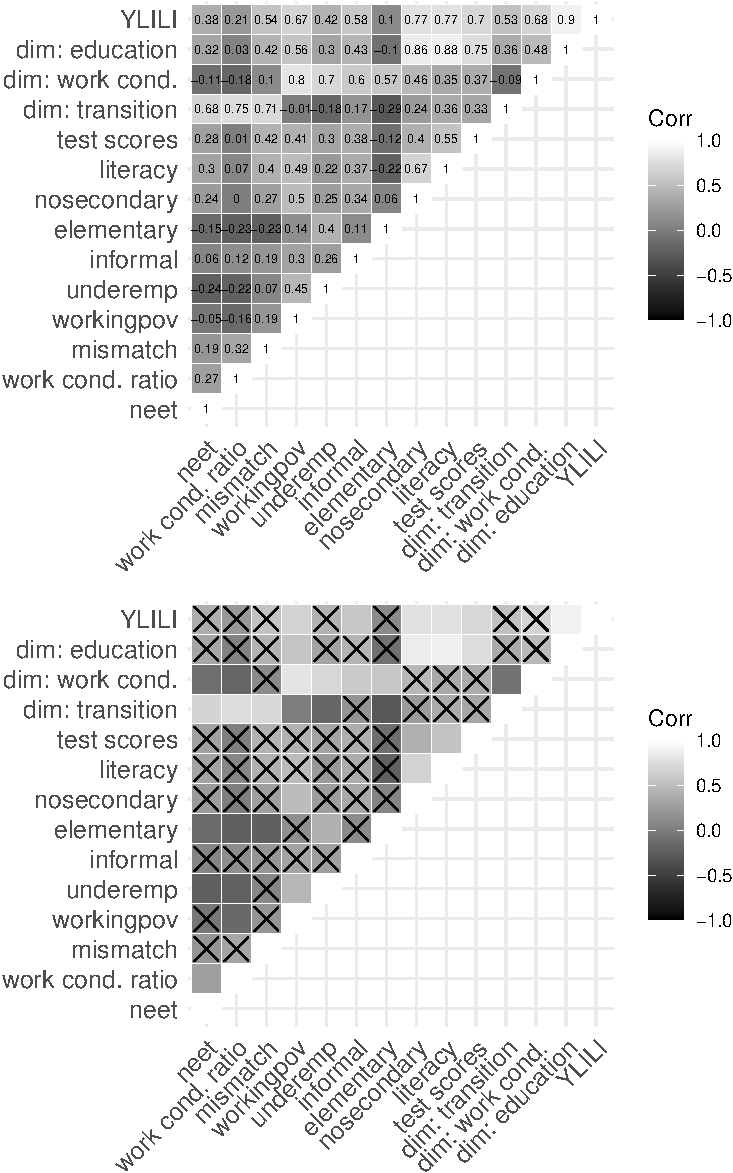
\includegraphics{figures/fig-cormat-1} 

}

\caption[Correlation matrix]{Correlation matrix (× = insignificant at p < 0.05)}\label{fig:fig-cormat}
\end{figure}

\newpage

\hypertarget{demographics}{%
\subsection*{Demographics by Income Level}\label{demographics}}

\begin{figure}[H]

{\centering 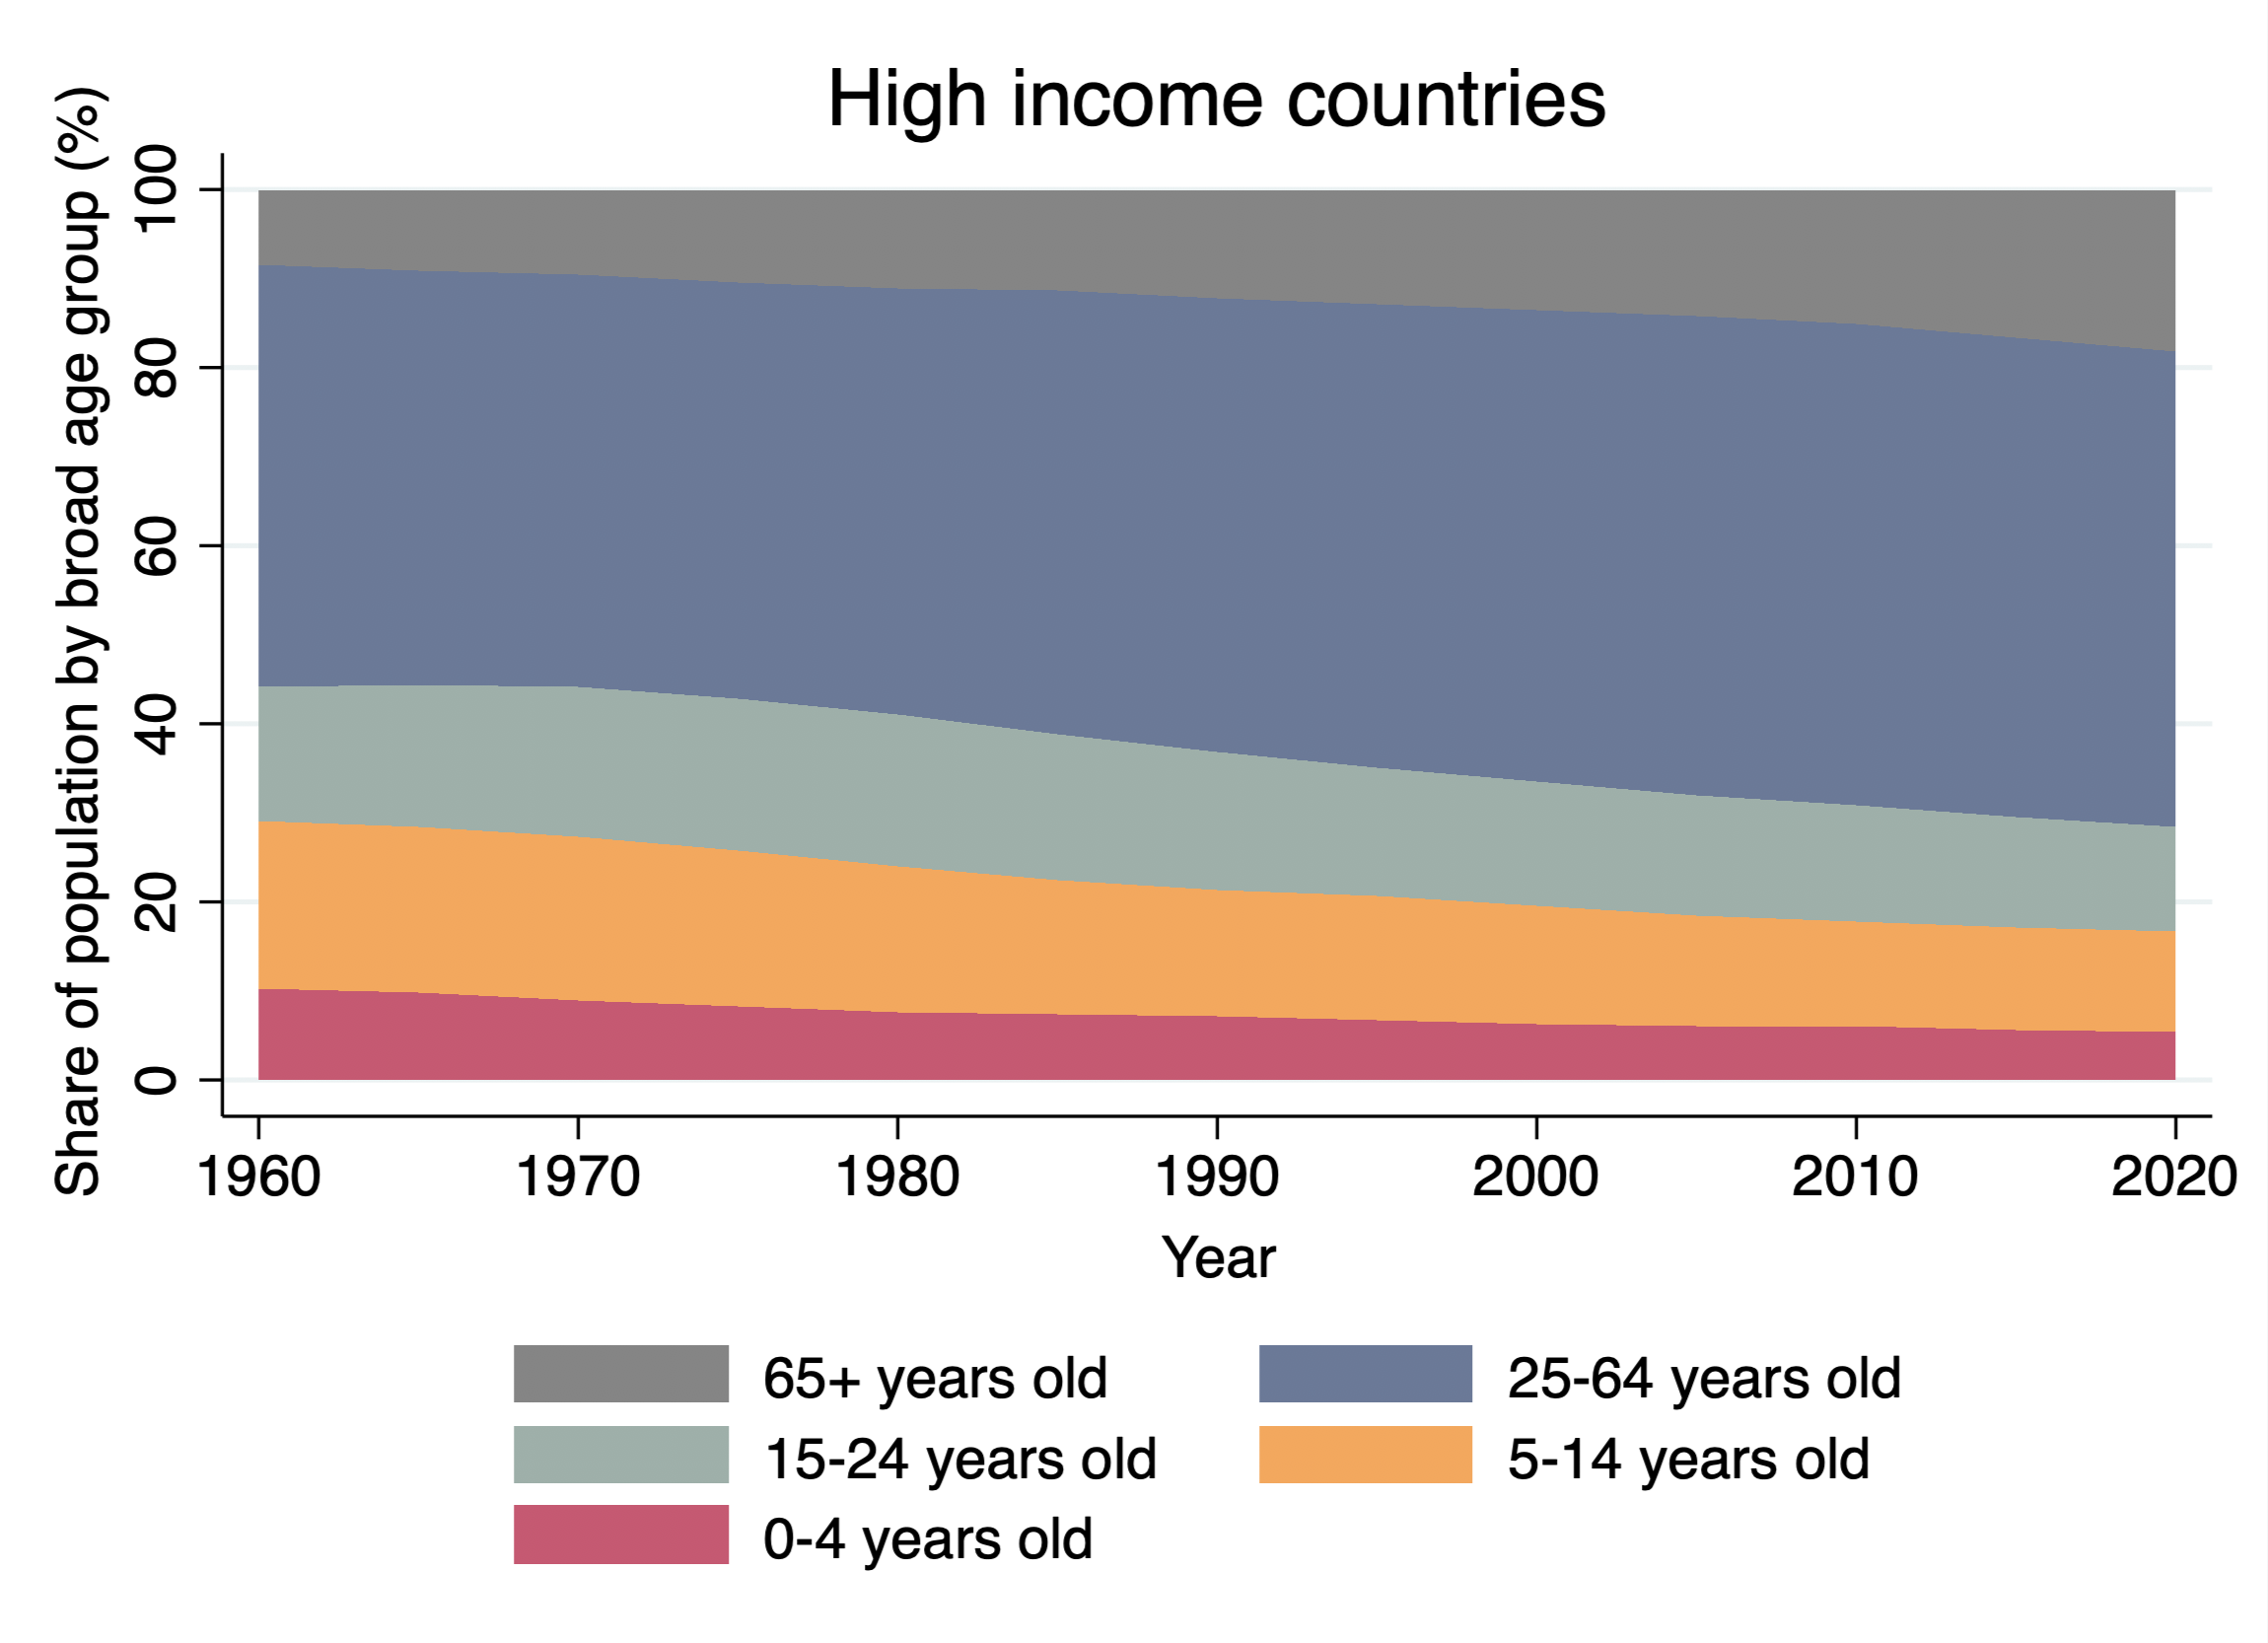
\includegraphics[width=0.43\linewidth,]{figures/stacked_highincome} 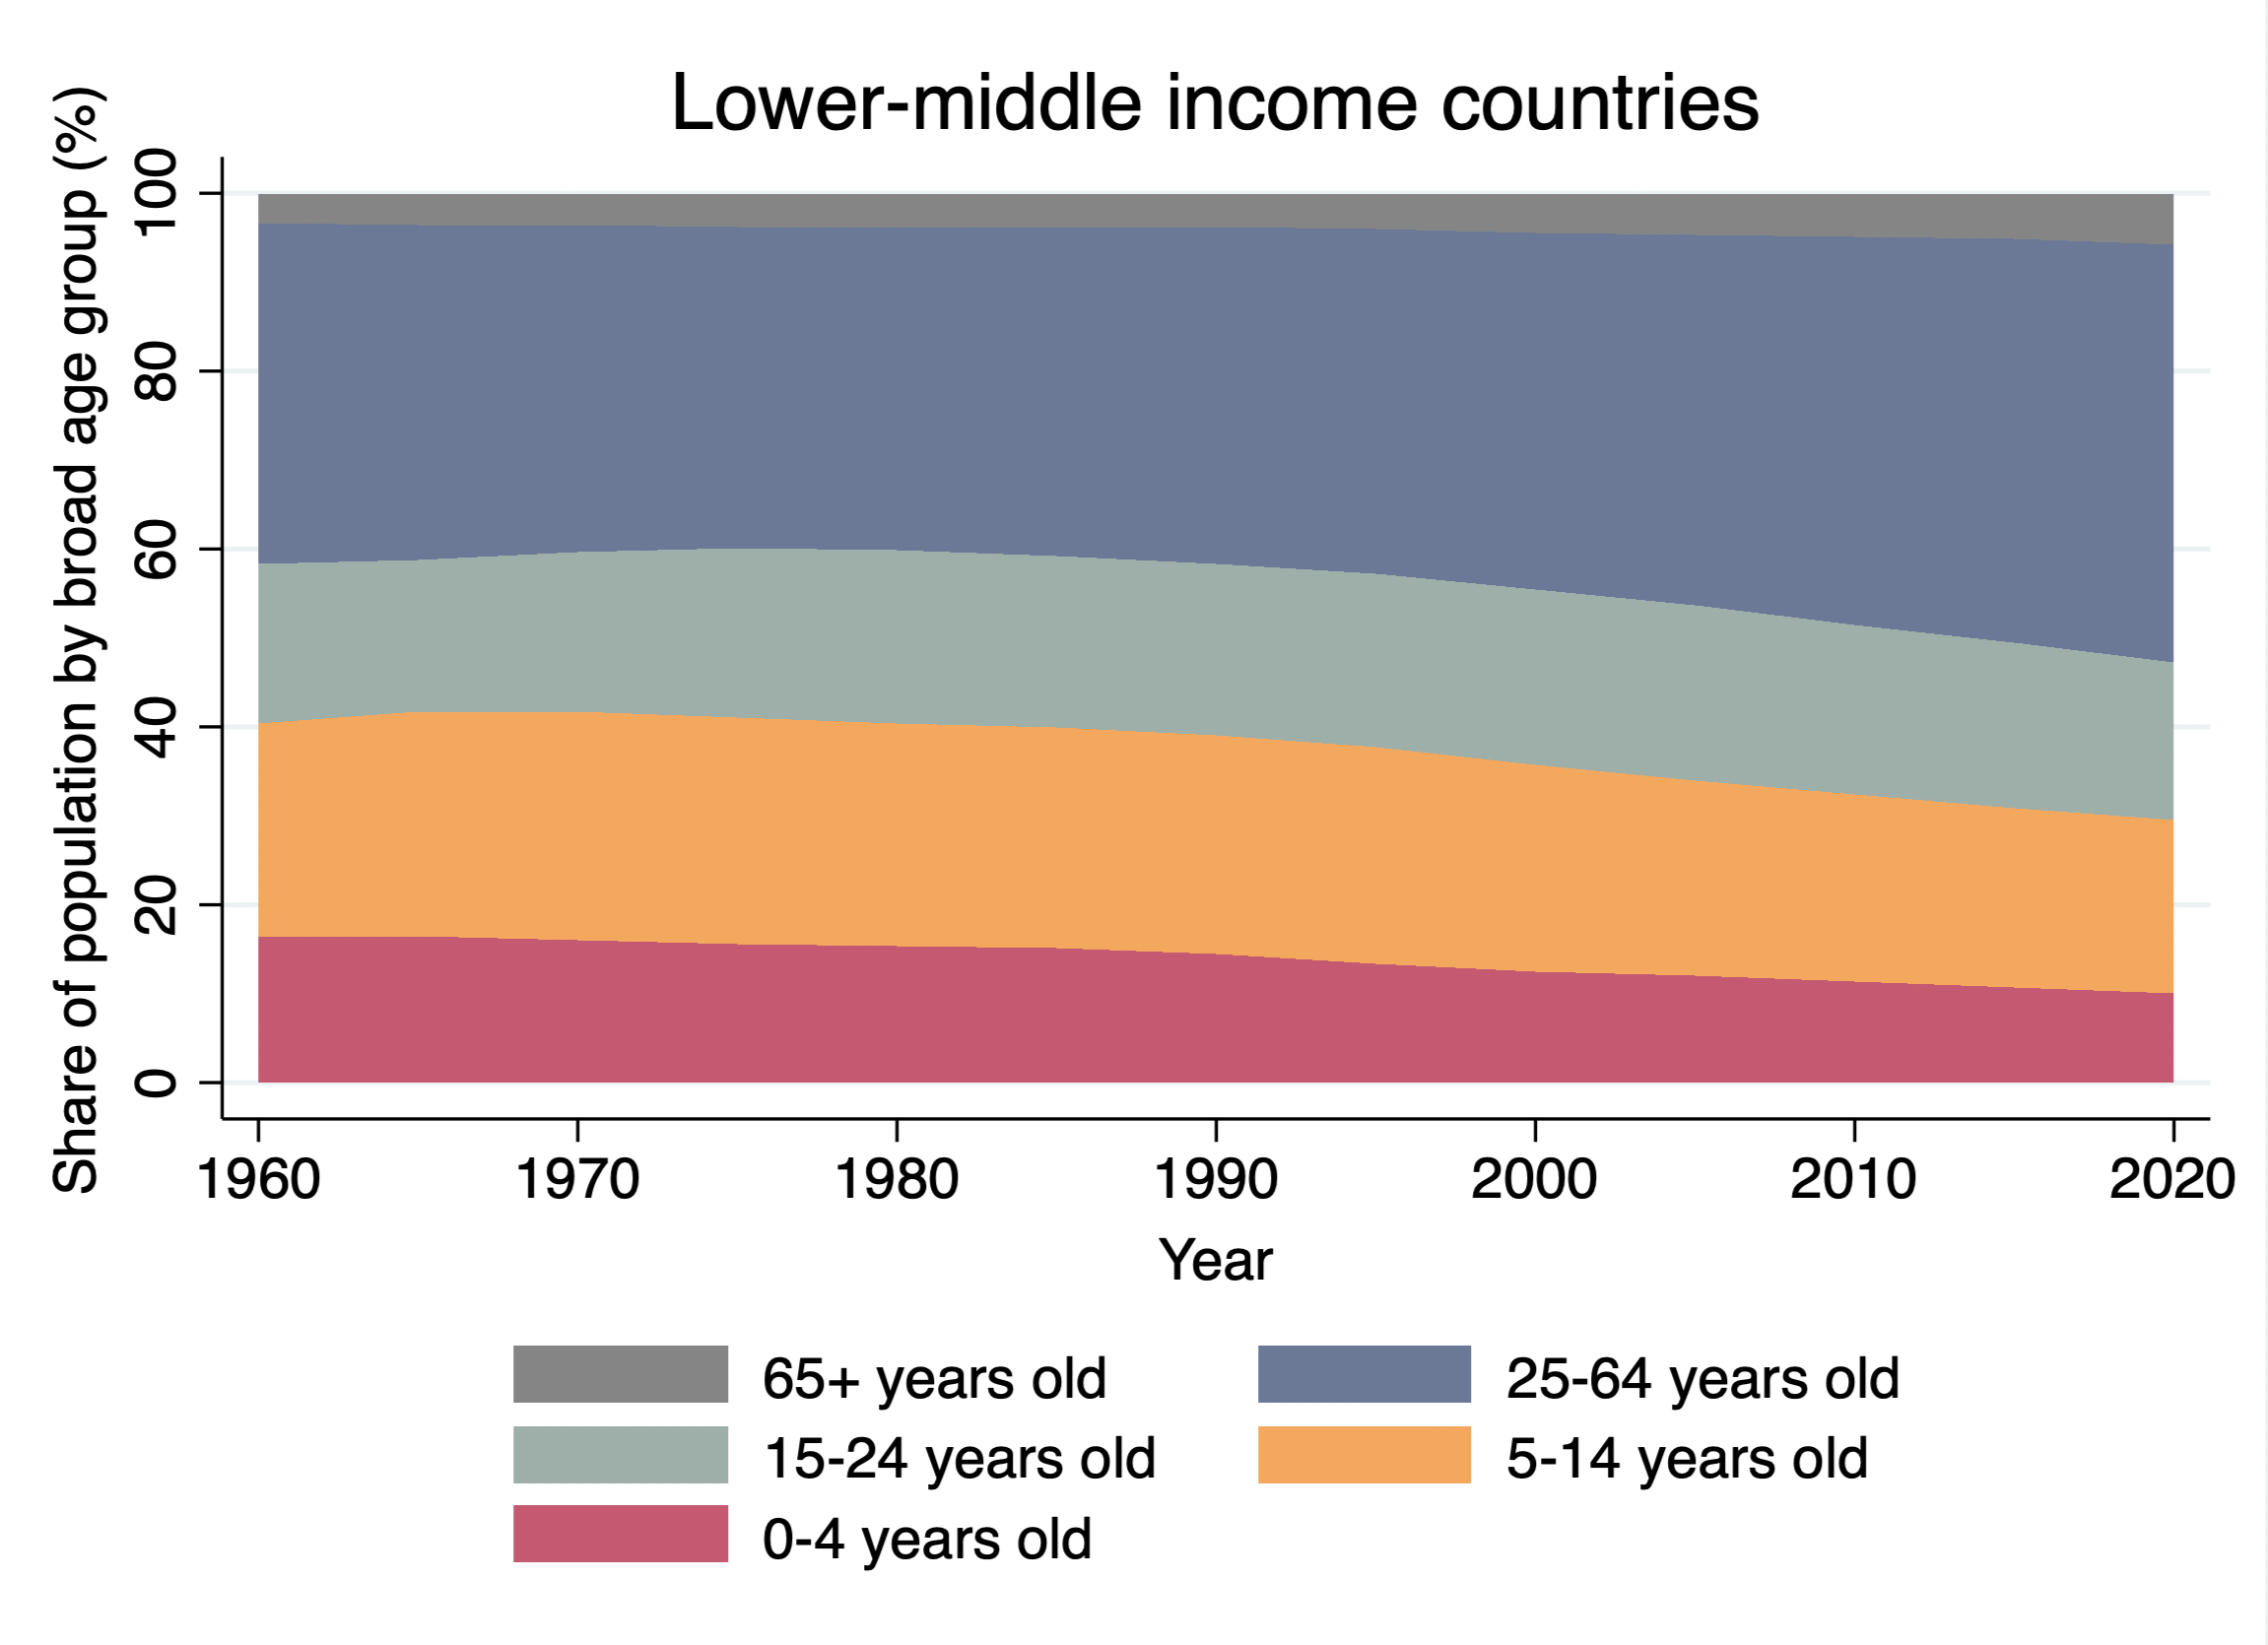
\includegraphics[width=0.43\linewidth,]{figures/stacked_lowermiddle} 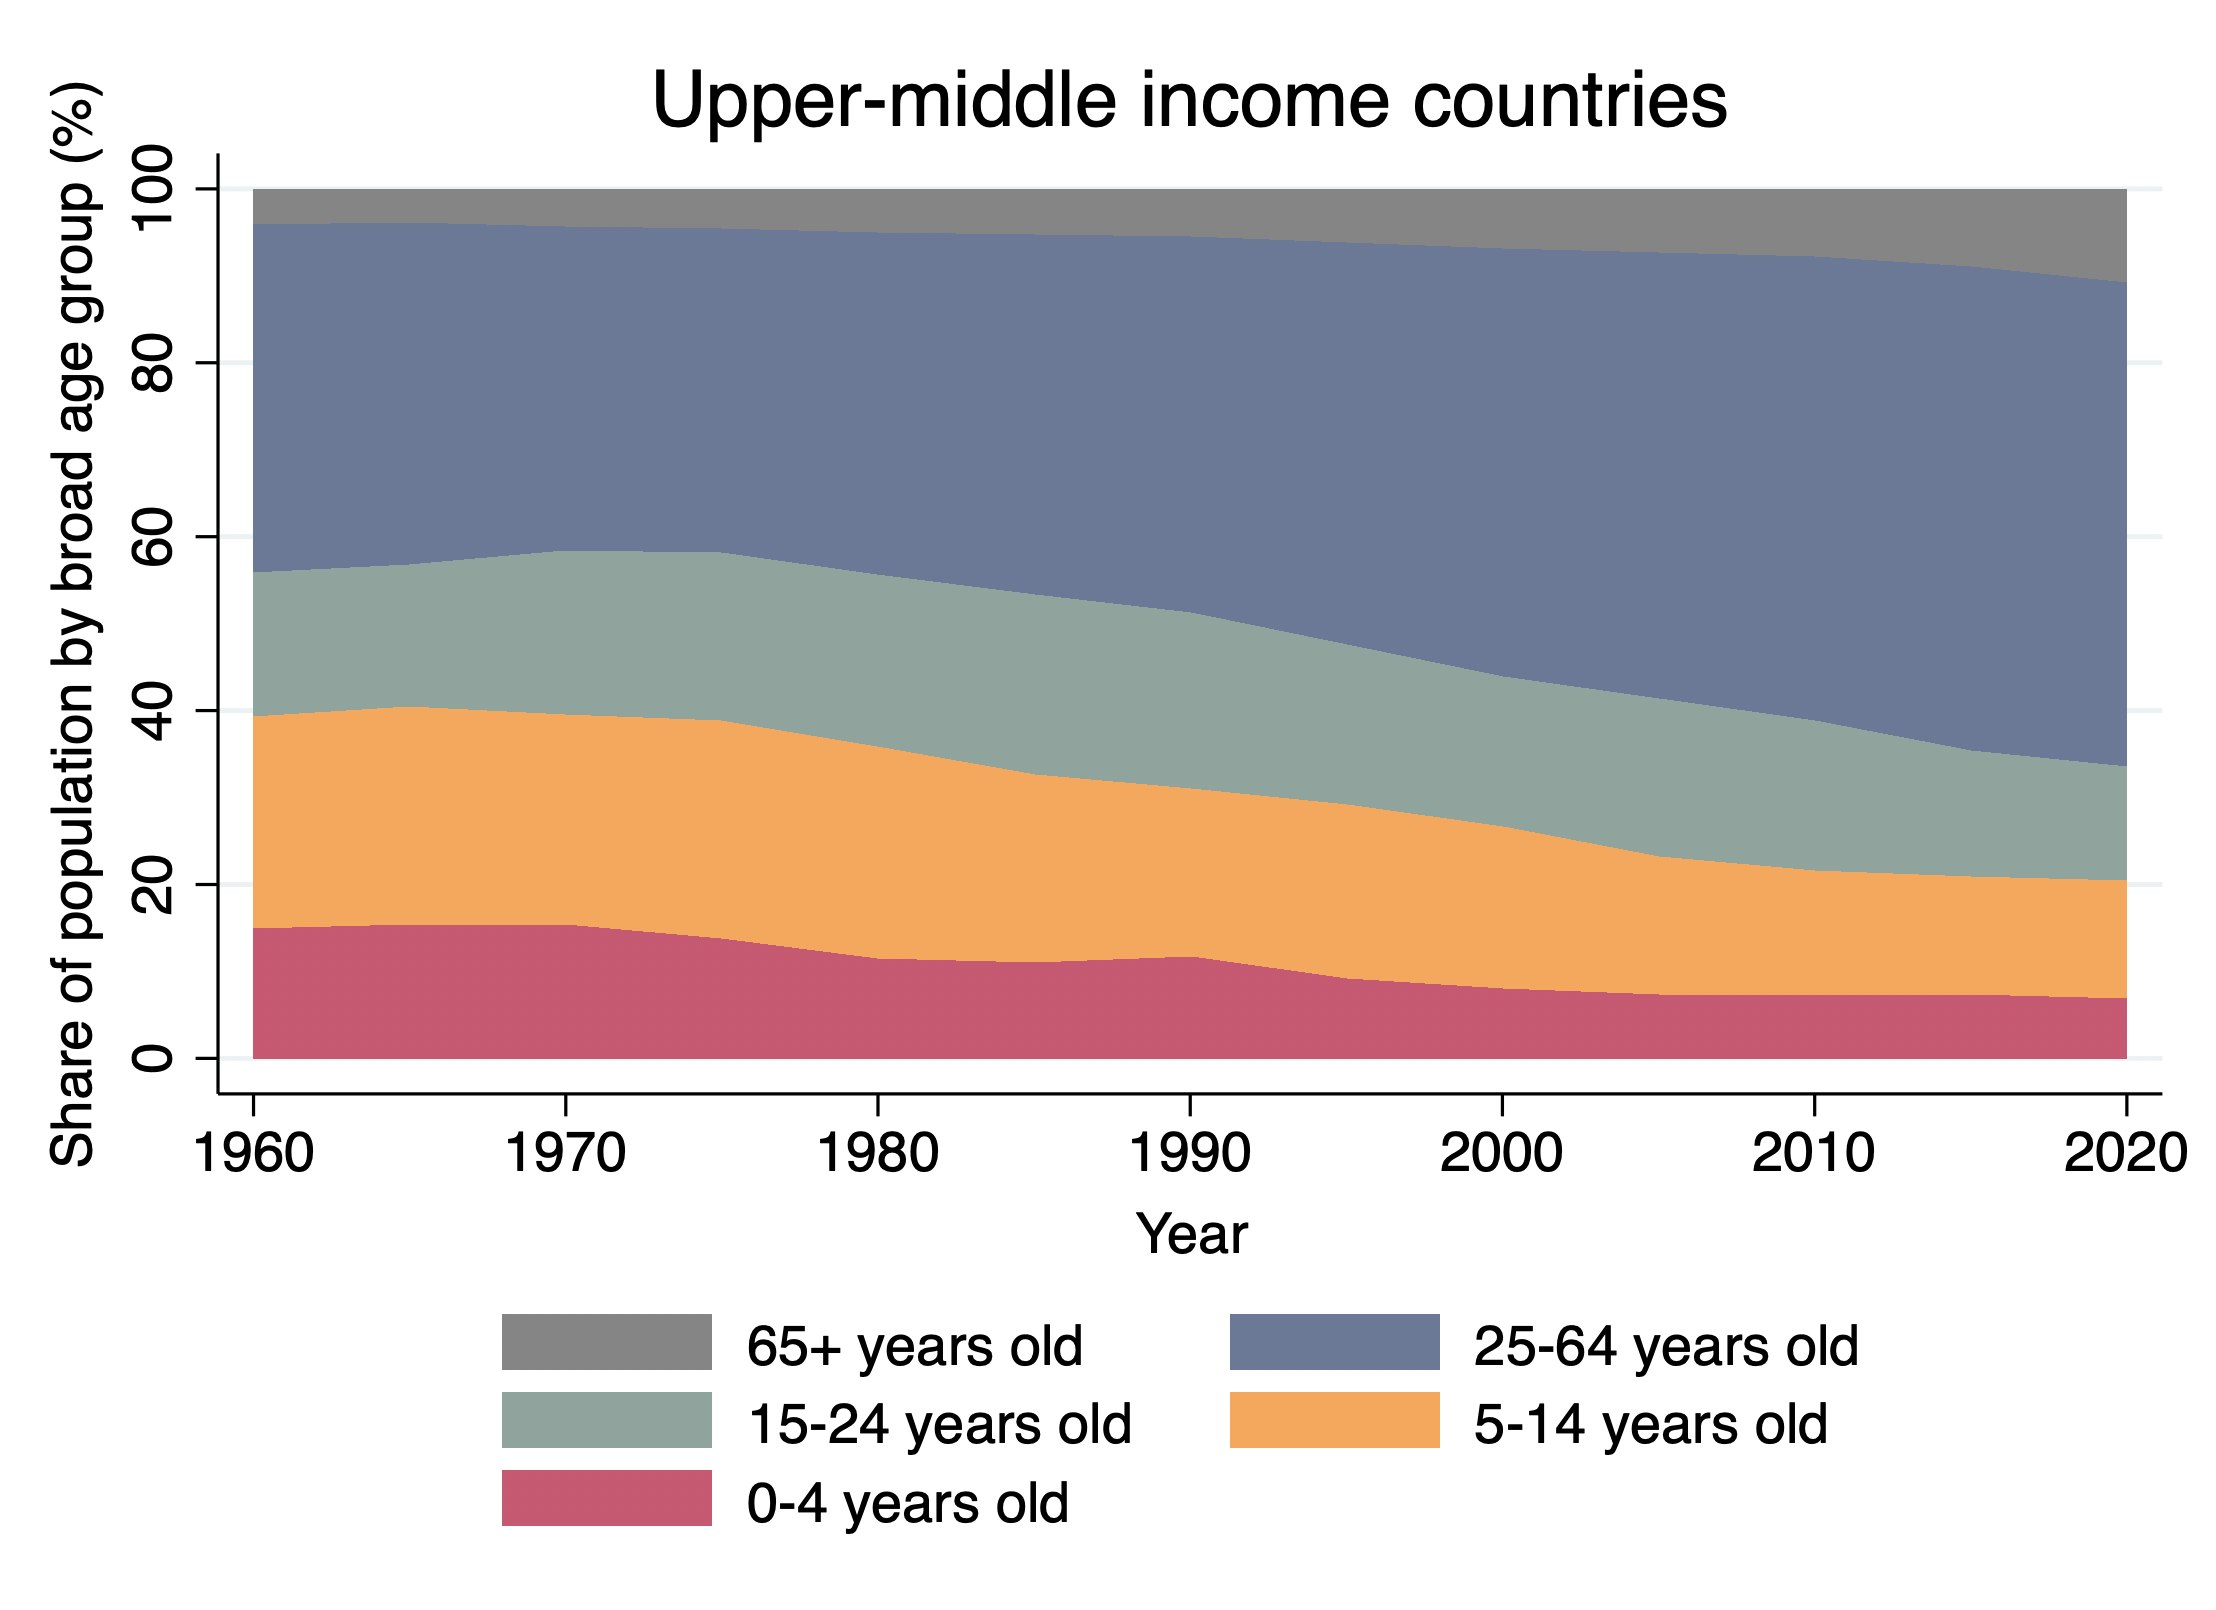
\includegraphics[width=0.43\linewidth,]{figures/stacked_highermiddle} 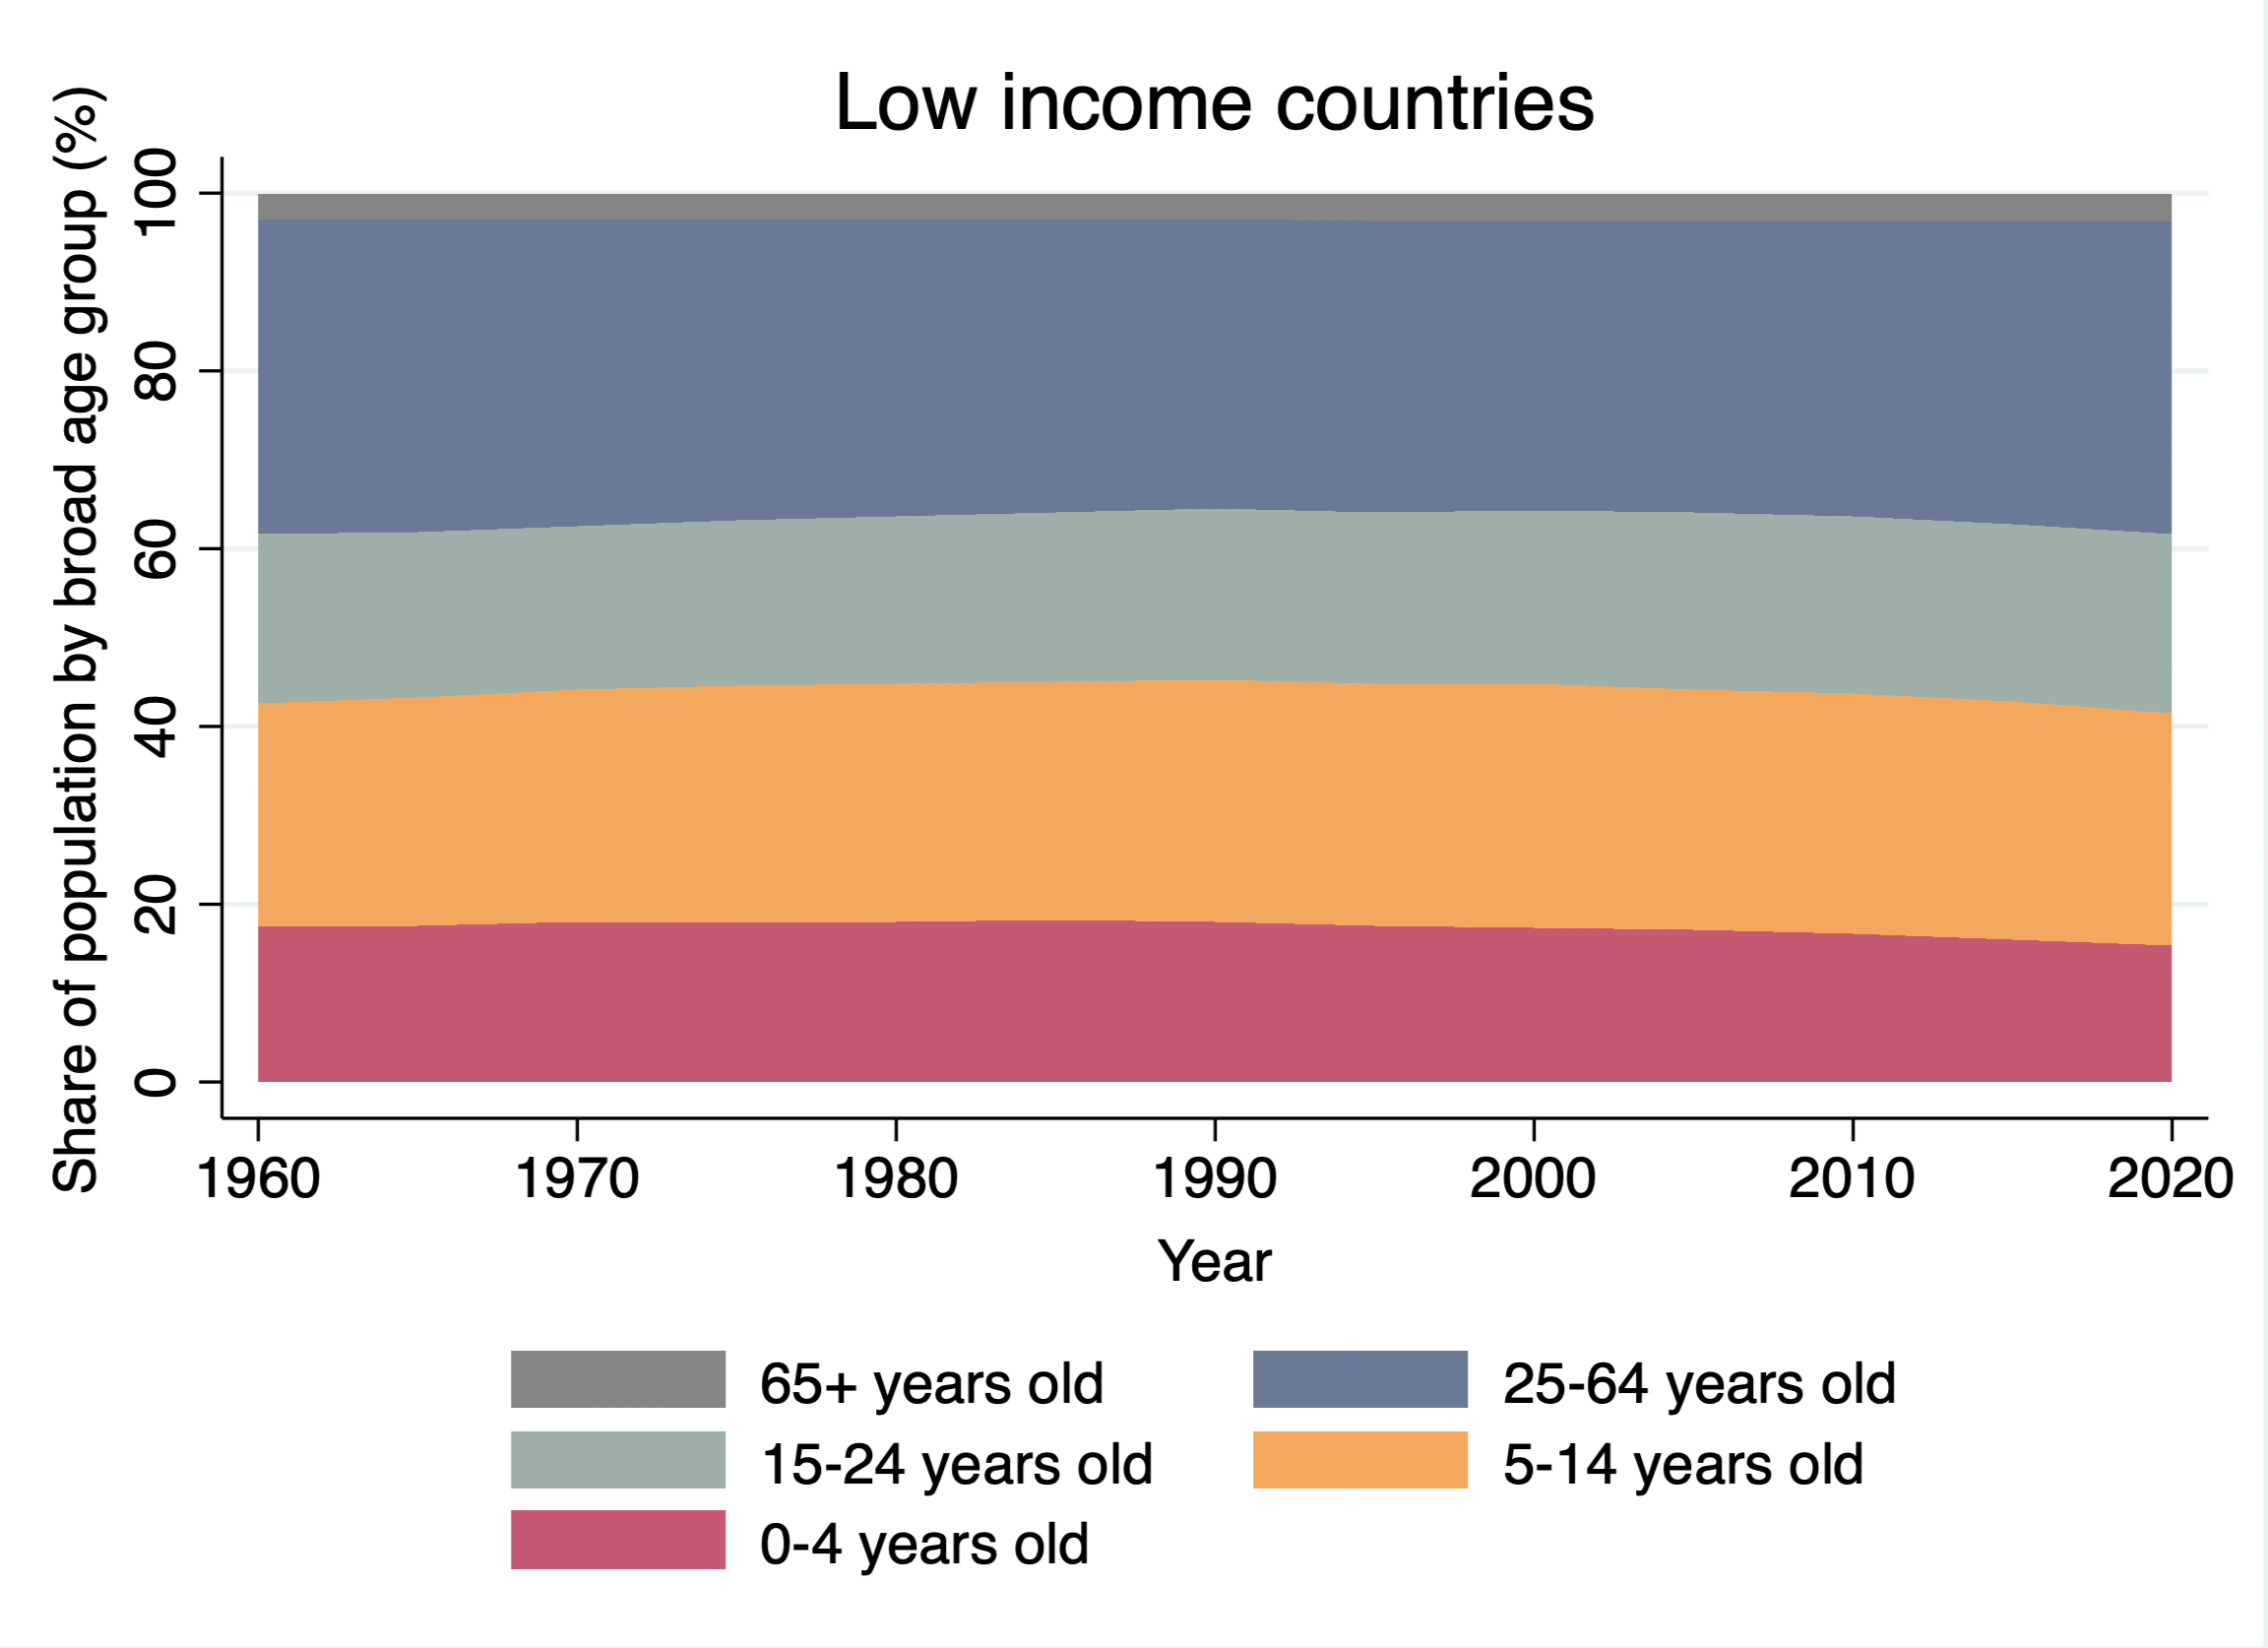
\includegraphics[width=0.43\linewidth,]{figures/stacked_lowincome} 

}

\caption[Share of world population by age group, 1960-2020]{Share of world population by age group, 1960-2020 \\ \textit{\footnotesize{Source: World Population Prospects, United Nations (2019)}}}\label{fig:fig-stacked}
\end{figure}

\begin{figure}[H]

{\centering 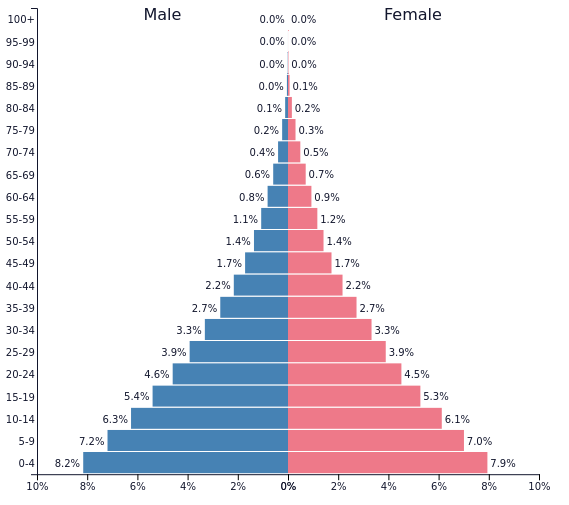
\includegraphics[width=0.43\linewidth,]{figures/pp_ssa} 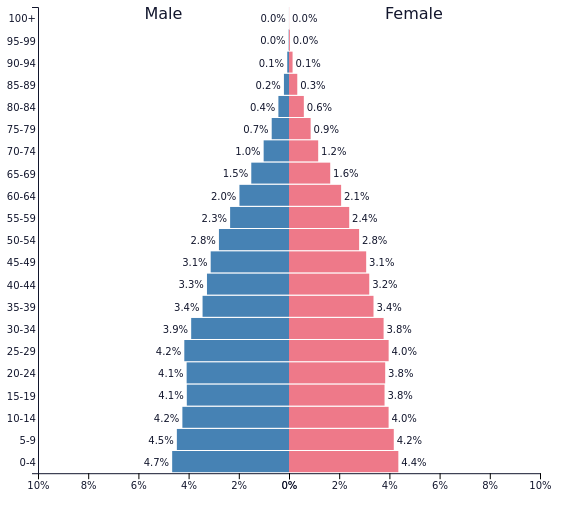
\includegraphics[width=0.43\linewidth,]{figures/pp_world} 

}

\caption[Population pyramids for sub-Saharan Africa]{Population pyramids for sub-Saharan Africa (left) vs. the world (right) \\ \textit{\footnotesize{Source: World Population Prospects, United Nations (2019)}}}\label{fig:fig-pyramids}
\end{figure}

\newpage

\hypertarget{appendix-b}{%
\section*{Appendix B2}\label{appendix-b}}
\addcontentsline{toc}{section}{Appendix B2}

\markboth{Appendix B2}{Appendix B2}

\setcounter{figure}{0}
\renewcommand{\thefigure}{B2.\arabic{figure}}
\setcounter{table}{0}
\renewcommand{\thetable}{B2.\arabic{table}}

\hypertarget{availability}{%
\subsection*{Availability of Indicators}\label{availability}}

\markboth{Availability of Indicators}{Appendix B2}

Table \ref{tab:tbl-kofcomp} shows the indicators included in the KOF Youth Labor Market Index \autocite{renold2014} and the corresponding YLILI indicator, if available. While grouping into dimensions remained roughly similar for the two indices, most indicators from the KOF YLMI were dropped or replaced in the YLILI, either for lack of availability or because more relevant indicators were needed for developing economies.

\begin{singlespacing}
\begin{table}[H]\caption{\textrm{\normalfont \small Comparison with KOF YLMI \label{tab:tbl-kofcomp}}}
\begin{adjustwidth}{-1cm}{}
 \centering
 \scalebox{.85}{
\begin{tabular}{c c l c c}
\hline\hline
&& \multicolumn{1}{c}{KOF Indicator} & \multicolumn{1}{c}{YLILI equivalent} & \multicolumn{1}{c}{Comment} \\
\hline
\parbox[t]{0mm}{\multirow{4}{*}{\rotatebox[origin=c]{90}{Transition}}} & \parbox[t]{2mm}{\multirow{4}{*}{\rotatebox[origin=c]{90}{smoothness}}} & \multirow{2}{*}{Relative unemployment ratio} & \multirow{2}{*}{Relative working conditions ratio} & \multicolumn{1}{c}{\multirow{2}{*}{---}}   \\
&& & & \\
&& Incidence of long-term & \multicolumn{1}{c}{\multirow{2}{*}{---}} & \multirow{2}{*}{Not appropriate} \\
&& unemployment rate & & \\
\hline
\parbox[t]{0mm}{\multirow{10}{*}{\rotatebox[origin=c]{90}{Working}}} & \parbox[t]{2mm}{\multirow{10}{*}{\rotatebox[origin=c]{90}{conditions}}}& \multirow{2}{*}{Temporary worker rate} & \multicolumn{1}{c}{\multirow{2}{*}{---}}  & \multirow{2}{*}{No data available} \\
&& & & \\
&& Involuntary part-time & \multicolumn{1}{c}{\multirow{2}{*}{---}}  & \multirow{2}{*}{No data available} \\
&& worker rate & & \\
&& \multirow{2}{*}{Atypical working hours rate} & \multicolumn{1}{c}{\multirow{2}{*}{---}}  & \multirow{2}{*}{No data available} \\
&& & & \\
&& In work, at risk of & \multirow{2}{*}{Working poverty rate}  & \multicolumn{1}{c}{\multirow{2}{*}{---}} \\
&& poverty rate & & \\
&& \multirow{2}{*}{Vulnerable employment rate} & \multirow{2}{*}{Vulnerable employment rate}  & \multicolumn{1}{c}{\multirow{2}{*}{---}} \\
&& & & \\
\hline
\parbox[t]{0mm}{\multirow{4}{*}{\rotatebox[origin=c]{90}{Education}}} & & Formal education and & \multicolumn{1}{c}{\multirow{2}{*}{---}} & No data available \\
&& training rate & & + not appropriate \\
&& \multirow{2}{*}{Skills mismatch rate} & \multirow{2}{*}{Skills mismatch rate}  & \multicolumn{1}{c}{\multirow{2}{*}{---}} \\
&& & & \\
\hline
\parbox[t]{0mm}{\multirow{6}{*}{\rotatebox[origin=c]{90}{Activity}}} & \parbox[t]{2mm}{\multirow{6}{*}{\rotatebox[origin=c]{90}{state}}} 
& \multirow{2}{*}{Unemployment rate} & \multicolumn{1}{c}{\multirow{2}{*}{---}}  & \multirow{2}{*}{Not appropriate} \\
&& & & \\
&& \multirow{2}{*}{Relaxed unemployment rate} & \multicolumn{1}{c}{\multirow{2}{*}{---}}  & \multirow{2}{*}{Not appropriate} \\
&& & & \\
&& \multirow{2}{*}{NEET rate} & \multirow{2}{*}{NEET rate}  & \multicolumn{1}{c}{\multirow{2}{*}{---}} \\
&& & & \\
\hline\hline
\end{tabular}}
\end{adjustwidth}
\end{table}
\end{singlespacing}

The availability of the indicators of the YLILI is highly scattered across countries and over time. For instance, data on the share of youth NEET is only available one year for Senegal, while it is available 12 years for Bolivia. To get around this issue, we compute the index by taking the last available year data was reported. It is possible that the last available year for indicators frequently date more than 10 years back, masking potential developments in labor market conditions and resulting in misleading comparisons. Hence we restrict the sample to data dating no further back than 2010. A trade-off thus exists between the number of countries for which the YLILI can be generated and the degree of conservatism of established rules regarding the set of indicators to include: the higher the number of countries for which the YLILI can be generated, the weaker the established rules and vice-versa.

Table \ref{tab:tbl-numind} shows the number of available indicators by year for all developing countries since the year 2000. Ideally, the country-year YLILI would have been generated by using all 10 indicators, i.e., the number of available indicators would have been equal to 10 for all 79 countries of the sample on a yearly basis. Unfortunately, limited administrative data on the labor market is a familiar problem across the developing world and Table \ref{tab:tbl-numind} confirms this: about half of the 79 countries analyzed for this index only have data on less than 3 indicators in any year and no country has all 10 indicators in any year since 2000.

\begin{singlespacing}
\begin{table}[H]\caption{\textrm{\normalfont \small Number of available indicators by year \label{tab:tbl-numind}}}
\begin{adjustwidth}{2cm}{}
\scalebox{0.9}{
\begin{tabular}{l|ccccccccccc|ccc}
\hline \hline 
\multirow{2}{*}{Year} & \multicolumn{10}{c}{Number of available indicators} & & Total number \\ 
& 0 & 1 & 2 & 3 & 4 & 5 & 6 & 7 & 8 & 9 & 10 & of countries \\ \hline
2020 & 10 & 66 &  1 & 0 & 0 &  2 & 0 & 0 & 0 & 0 & 0 & 79 \\ 
  2019 &  4 & 51 &  6 &  6 & 0 &  5 &  6 &  1 & 0 & 0 & 0 & 79 \\ 
  2018 &  2 &  7 & 27 & 19 &  5 &  2 &  3 &  6 &  7 &  1 & 0 & 79 \\ 
  2017 &  2 & 10 & 28 &  9 &  5 &  4 &  3 &  9 &  5 &  4 & 0 & 79 \\ 
  2016 &  6 & 40 & 14 &  5 &  1 &  4 &  4 &  5 & 0 & 0 & 0 & 79 \\ 
  2015 &  5 & 34 & 17 &  5 &  3 &  5 &  4 &  5 &  1 & 0 & 0 & 79 \\ 
  2014 &  4 & 28 & 13 &  7 &  8 &  6 &  9 &  2 &  1 &  1 & 0 & 79 \\ 
  2013 &  6 & 33 & 11 &  9 &  5 &  5 &  4 &  6 & 0 & 0 & 0 & 79 \\ 
  2012 &  5 & 33 &  9 & 11 &  6 &  6 &  6 &  2 &  1 & 0 & 0 & 79 \\ 
  2011 &  6 & 34 & 13 &  7 &  7 &  3 &  5 &  2 &  2 & 0 & 0 & 79 \\ 
  2010 &  5 & 32 & 15 & 10 &  5 &  2 &  9 &  1 & 0 & 0 & 0 & 79 \\ 
  2009 &  5 & 45 &  9 &  5 &  7 &  4 &  4 & 0 & 0 & 0 & 0 & 79 \\ 
  2008 &  4 & 51 & 13 &  4 &  1 &  3 &  2 & 0 &  1 & 0 & 0 & 79 \\ 
  2007 &  6 & 50 & 10 &  6 &  3 & 0 &  3 &  1 & 0 & 0 & 0 & 79 \\ 
  2006 &  5 & 46 & 15 &  5 &  4 &  2 &  2 & 0 & 0 & 0 & 0 & 79 \\ 
  2005 &  6 & 45 & 19 &  3 &  1 &  3 &  2 & 0 & 0 & 0 & 0 & 79 \\ 
  2004 &  5 & 55 & 15 &  3 &  1 & 0 & 0 & 0 & 0 & 0 & 0 & 79 \\ 
  2003 &  6 & 59 &  8 &  6 & 0 & 0 & 0 & 0 & 0 & 0 & 0 & 79 \\ 
  2002 &  6 & 62 & 10 &  1 & 0 & 0 & 0 & 0 & 0 & 0 & 0 & 79 \\ 
  2001 &  5 & 56 & 13 &  3 &  1 &  1 & 0 & 0 & 0 & 0 & 0 & 79 \\ 
  2000 &  6 & 38 & 29 &  4 &  2 & 0 & 0 & 0 & 0 & 0 & 0 & 79 \\   \hline \hline
\end{tabular}}
\end{adjustwidth}
\end{table} 


\end{singlespacing}

Despite this sample restriction, one obvious limitation is that distinct years are pooled together, which prevents comparisons within and between countries over time. On the other hand, the major advantage of this method is that it includes the maximum possible number of indicators for each country and hence exploits all the available information. Table \ref{tab:tbl-coverage} provides an overview of the coverage of each indicator by year since 2010. The table shows that the last available year of the vast majority of indicators date no further back than 2014. For instance, more than 80\% of countries gathered data for the share of youth NEET since 2014 (among those who did gather data for the share of youth NEET since 2010).

\begin{table}[H]\caption{Coverage of indicators (\%) by year, last available year \label{tab:tbl-coverage}}
\centering
\begin{adjustwidth}{1.5cm}{}
 \scalebox{0.8}{
\begin{tabular}{l|cccccccccccccccc}
\rot{Year} & \rot{Share of youth NEET} & \rot{Relative working conditions ratio} & \rot{Youth skills mismatch rate} & \rot{Youth working poverty rate} & \rot{Youth time-related under. rate} & \rot{Share of youth in informal emp.} & \rot{Share of youth work. in EO} & \rot{Share of youth with no sec. educ.} & \rot{Youth illiteracy rate} & \rot{Harmonized test scores} \\ \hline
2010 & 3.08  & 6.12         & 1.85     & 0.00       & 5.45     & 5.88     & 0.00       & 2.38        & 1.41     & 0.00         \\
2011 & 3.08  & 2.04         & 7.41     & 0.00       & 1.82     & 9.80     & 0.00       & 9.52        & 0.00     & 0.00         \\
2012 & 3.08  & 6.12         & 5.56     & 0.00       & 5.45     & 11.76    & 1.85       & 7.14        & 1.41     & 0.00         \\
2013 & 3.08  & 8.16         & 9.26     & 0.00       & 7.27     & 11.76    & 9.26       & 7.14        & 0.00     & 0.00         \\
2014 & 12.31 & 16.33        & 14.81    & 0.00       & 14.55    & 17.65    & 11.11      & 14.29       & 9.86     & 0.00         \\
2015 & 1.54  & 2.04         & 3.70     & 0.00       & 1.82     & 7.84     & 11.11      & 19.05       & 14.08    & 0.00         \\
2016 & 6.15  & 2.04         & 3.70     & 0.00       & 5.45     & 7.84     & 1.85       & 16.67       & 5.63     & 0.00         \\
2017 & 26.15 & 20.41        & 22.22    & 0.00       & 20.00    & 23.53    & 20.37      & 4.76        & 12.68    & 0.00         \\
2018 & 13.85 & 14.29        & 11.11    & 0.00       & 12.73    & 3.92     & 12.96      & 11.90       & 52.11    & 0.00         \\
2019 & 24.62 & 22.45        & 16.67    & 100.00     & 21.82    & 0.00     & 25.93      & 7.14        & 2.82     & 0.00         \\
2020 & 3.08  & 0.00         & 3.70     & 0.00       & 3.64     & 0.00     & 5.56       & 0.00        & 0.00     & 100.00      \\\hline \hline
\end{tabular}}
\end{adjustwidth}
\end{table}

Finally, Table \ref{tab:tbl-avail} indicates how many indicators were utilized to compute the YLILI score for each country. In theory, the maximum possible number of indicators is 10. However, because of data availability, the number of indicators utilized to compute the index varies between countries. In order to take into consideration all dimensions of the labor market and to generate an index as comparable as possible between countries while maximizing the number of countries, we decide that the index can only be generated if there are a minimum of 2 indicators in the transition and education dimensions and 3 indicators in the working condition dimension (7 indicators in total). Table \ref{tab:tbl-avail} shows that the vast majority of countries comprise at least 7 out of 10 indicators (\(>80\%\) of indicators), however, we advise that interpretations from the index should be made with caution. Overall, the YLILI could be computed for 54 out of 79 countries.

\begin{singlespacing}
\newpage
\begin{singlespace}
\begingroup
\renewcommand*{\arraystretch}{1.241}
\setlength\LTleft{+3cm}
 \footnotesize{
\begin{longtable}{l l c c c c c c c c} 
\caption{\textrm{\normalfont \small Availability of indicators, last available year \label{tab:tbl-avail}}} 
\\ \hline \hline
\rot{Country name}    & \rot{Country abbreviation} & \rot{Transition (\# out of 3)} & \rot{Working cond. (\# out of 4)} & \rot{Education (\# out of 3)} & \rot{Total \# of indicators} & \rot{YLILI computed?} \\ \hline
Benin                      & BEN           & 3          & 4                   & 3         & 10                & Yes             \\
Burkina Faso               & BFA           & 3          & 4                   & 3         & 10                & Yes             \\
Bangladesh                 & BGD           & 3          & 4                   & 3         & 10                & Yes             \\
Ivory Coast                & CIV           & 3          & 4                   & 3         & 10                & Yes             \\
Cameroon                   & CMR           & 3          & 4                   & 3         & 10                & Yes             \\
Ethiopia                   & ETH           & 3          & 4                   & 3         & 10                & Yes             \\
Ghana                      & GHA           & 3          & 4                   & 3         & 10                & Yes             \\
Gambia                     & GMB           & 3          & 4                   & 3         & 10                & Yes             \\
Honduras                   & HND           & 3          & 4                   & 3         & 10                & Yes             \\
Cambodia                   & KHM           & 3          & 4                   & 3         & 10                & Yes             \\
Myanmar                    & MMR           & 3          & 4                   & 3         & 10                & Yes             \\
Nepal                      & NPL           & 3          & 4                   & 3         & 10                & Yes             \\
Pakistan                   & PAK           & 3          & 4                   & 3         & 10                & Yes             \\
Rwanda                     & RWA           & 3          & 4                   & 3         & 10                & Yes             \\
Senegal                    & SEN           & 3          & 4                   & 3         & 10                & Yes             \\
Togo                       & TGO           & 3          & 4                   & 3         & 10                & Yes             \\
Timor-Leste                & TLS           & 3          & 4                   & 3         & 10                & Yes             \\
Tanzania                   & TZA           & 3          & 4                   & 3         & 10                & Yes             \\
Uganda                     & UGA           & 3          & 4                   & 3         & 10                & Yes             \\
Zambia                     & ZMB           & 3          & 4                   & 3         & 10                & Yes             \\
Zimbabwe                   & ZWE           & 3          & 4                   & 3         & 10                & Yes             \\
Afghanistan                & AFG           & 3          & 3                   & 3         & 9                 & Yes             \\
Egypt                      & EGY           & 3          & 4                   & 2         & 9                 & Yes             \\
Kyrgyzstan                 & KGZ           & 2          & 4                   & 3         & 9                 & Yes             \\
Lao PDR                    & LAO           & 3          & 4                   & 2         & 9                 & Yes             \\
Liberia                    & LBR           & 2          & 4                   & 3         & 9                 & Yes             \\
Sri Lanka                  & LKA           & 3          & 4                   & 2         & 9                 & Yes             \\
Moldova                    & MDA           & 3          & 4                   & 2         & 9                 & Yes             \\
Madagascar                 & MDG           & 3          & 4                   & 2         & 9                 & Yes             \\
Mali                       & MLI           & 2          & 4                   & 3         & 9                 & Yes             \\
Mongolia                   & MNG           & 3          & 4                   & 2         & 9                 & Yes             \\
Mozambique                 & MOZ           & 2          & 4                   & 3         & 9                 & Yes             \\
Philippines                & PHL           & 3          & 4                   & 2         & 9                 & Yes             \\
Occupied Palestinian & \multirow{2}{*}{PSE}           & \multirow{2}{*}{3}          & \multirow{2}{*}{4}                   & \multirow{2}{*}{2}         & \multirow{2}{*}{9}                 & \multirow{2}{*}{Yes}             \\
Territory \\
Sierra Leone               & SLE           & 2          & 4                   & 3         & 9                 & Yes             \\
El Salvador                & SLV           & 3          & 4                   & 2         & 9                 & Yes             \\
Viet Nam                   & VNM           & 3          & 4                   & 2         & 9                 & Yes             \\
Burundi                    & BDI           & 2          & 3                   & 3         & 8                 & Yes             \\
Congo DR                   & COD           & 2          & 3                   & 3         & 8                 & Yes             \\
Comoros                    & COM           & 3          & 2                   & 3         & 8                 & Yes             \\
Haiti                      & HTI           & 3          & 2                   & 3         & 8                 & Yes             \\
Lesotho                    & LSO           & 2          & 3                   & 3         & 8                 & Yes             \\
Mauritania                 & MRT           & 3          & 3                   & 2         & 8                 & Yes             \\
Malawi                     & MWI           & 2          & 3                   & 3         & 8                 & Yes             \\
Niger                      & NER           & 2          & 3                   & 3         & 8                 & Yes             \\
Nicaragua                  & NIC           & 3          & 3                   & 2         & 8                 & Yes             \\
Angola                     & AGO           & 2          & 2                   & 3         & 7                 & Yes             \\
India                      & IND           & 2          & 2                   & 3         & 7                 & Yes             \\
Nigeria                    & NGA           & 2          & 2                   & 3         & 7                 & Yes             \\
Tunisia                    & TUN           & 2          & 3                   & 2         & 7                 & Yes             \\
Ukraine                    & UKR           & 2          & 3                   & 2         & 7                 & Yes             \\
Bhutan                     & BTN           & 2          & 2                   & 2         & 6                 & Yes             \\
Algeria                    & DZA           & 2          & 2                   & 2         & 6                 & Yes             \\
Sudan                      & SDN           & 2          & 2                   & 2         & 6                 & Yes             \\
Bolivia                    & BOL           & 3          & 4                   & 1         & 8                 & No              \\
Cape Verde                 & CPV           & 3          & 4                   & 1         & 8                 & No              \\
Eswatini                   & SWZ           & 1          & 4                   & 2         & 7                 & No              \\
Yemen                      & YEM           & 3          & 3                   & 1         & 7                 & No              \\
Guinea                     & GIN           & 1          & 2                   & 3         & 6                 & No              \\
Kenya                      & KEN           & 2          & 1                   & 3         & 6                 & No              \\
Morocco                    & MAR           & 1          & 3                   & 2         & 6                 & No              \\
Papua New Guinea           & PNG           & 2          & 1                   & 3         & 6                 & No              \\
Solomon Islands            & SLB           & 2          & 3                   & 1         & 6                 & No              \\
Chad                       & TCD           & 1          & 2                   & 3         & 6                 & No              \\
Vanuatu                    & VUT           & 1          & 2                   & 2         & 5                 & No              \\
Congo                      & COG           & 0          & 1                   & 3         & 4                 & No              \\
Kiribati                   & KIR           & 1          & 2                   & 1         & 4                 & No              \\
Central African Republic   & CAF           & 0          & 1                   & 2         & 3                 & No              \\
Djibouti                   & DJI           & 2          & 1                   & 0         & 3                 & No              \\
Micronesia                 & FSM           & 1          & 2                   & 0         & 3                 & No              \\
Tajikistan                 & TJK           & 0          & 1                   & 2         & 3                 & No              \\
Uzbekistan                 & UZB           & 0          & 1                   & 2         & 3                 & No              \\
Eritrea                    & ERI           & 0          & 1                   & 1         & 2                 & No              \\
Guinea-Bissau              & GNB           & 0          & 1                   & 1         & 2                 & No              \\
South Sudan                & SSD           & 0          & 0                   & 2         & 2                 & No              \\
Korea DPR                  & PRK           & 0          & 1                   & 0         & 1                 & No              \\
Somalia                    & SOM           & 0          & 1                   & 0         & 1                 & No              \\
Sao Tome and Principe      & STP           & 0          & 0                   & 1         & 1                 & No              \\
Syrian Arab Republic       & SYR           & 0          & 1                   & 0         & 1                 & No             
\\ \hline \hline
\end{longtable}
}
\endgroup
\end{singlespace}

\end{singlespacing}

\hypertarget{maps}{%
\subsection*{Geographic distribution of YLILI scores}\label{maps}}

\markboth{Geographic distribution of YLILI scores}{Appendix B2}

\begin{figure}[H]

{\centering 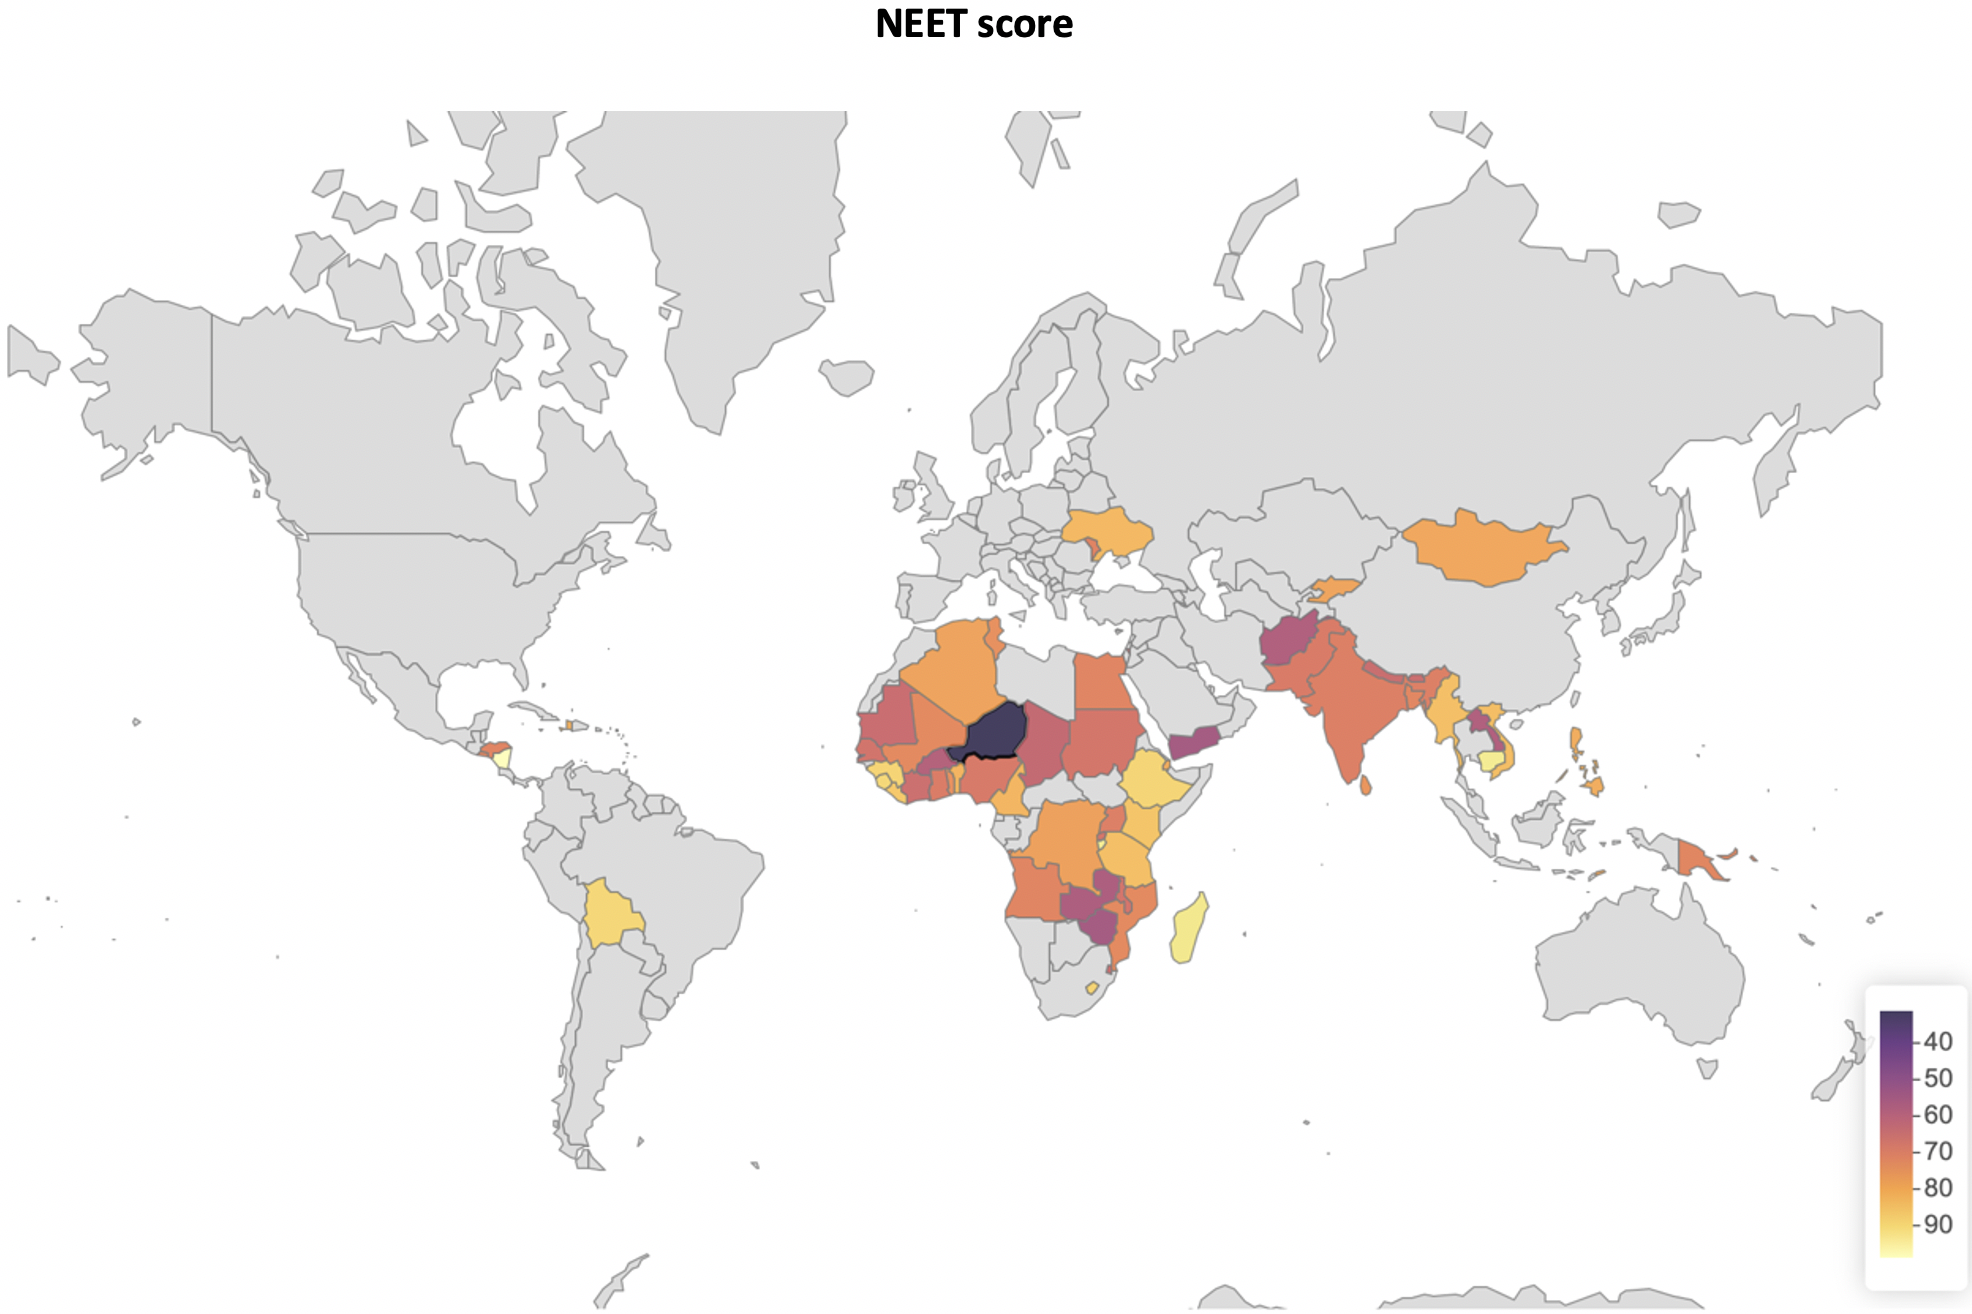
\includegraphics[width=0.7\linewidth,]{figures/maps/NEET_total} 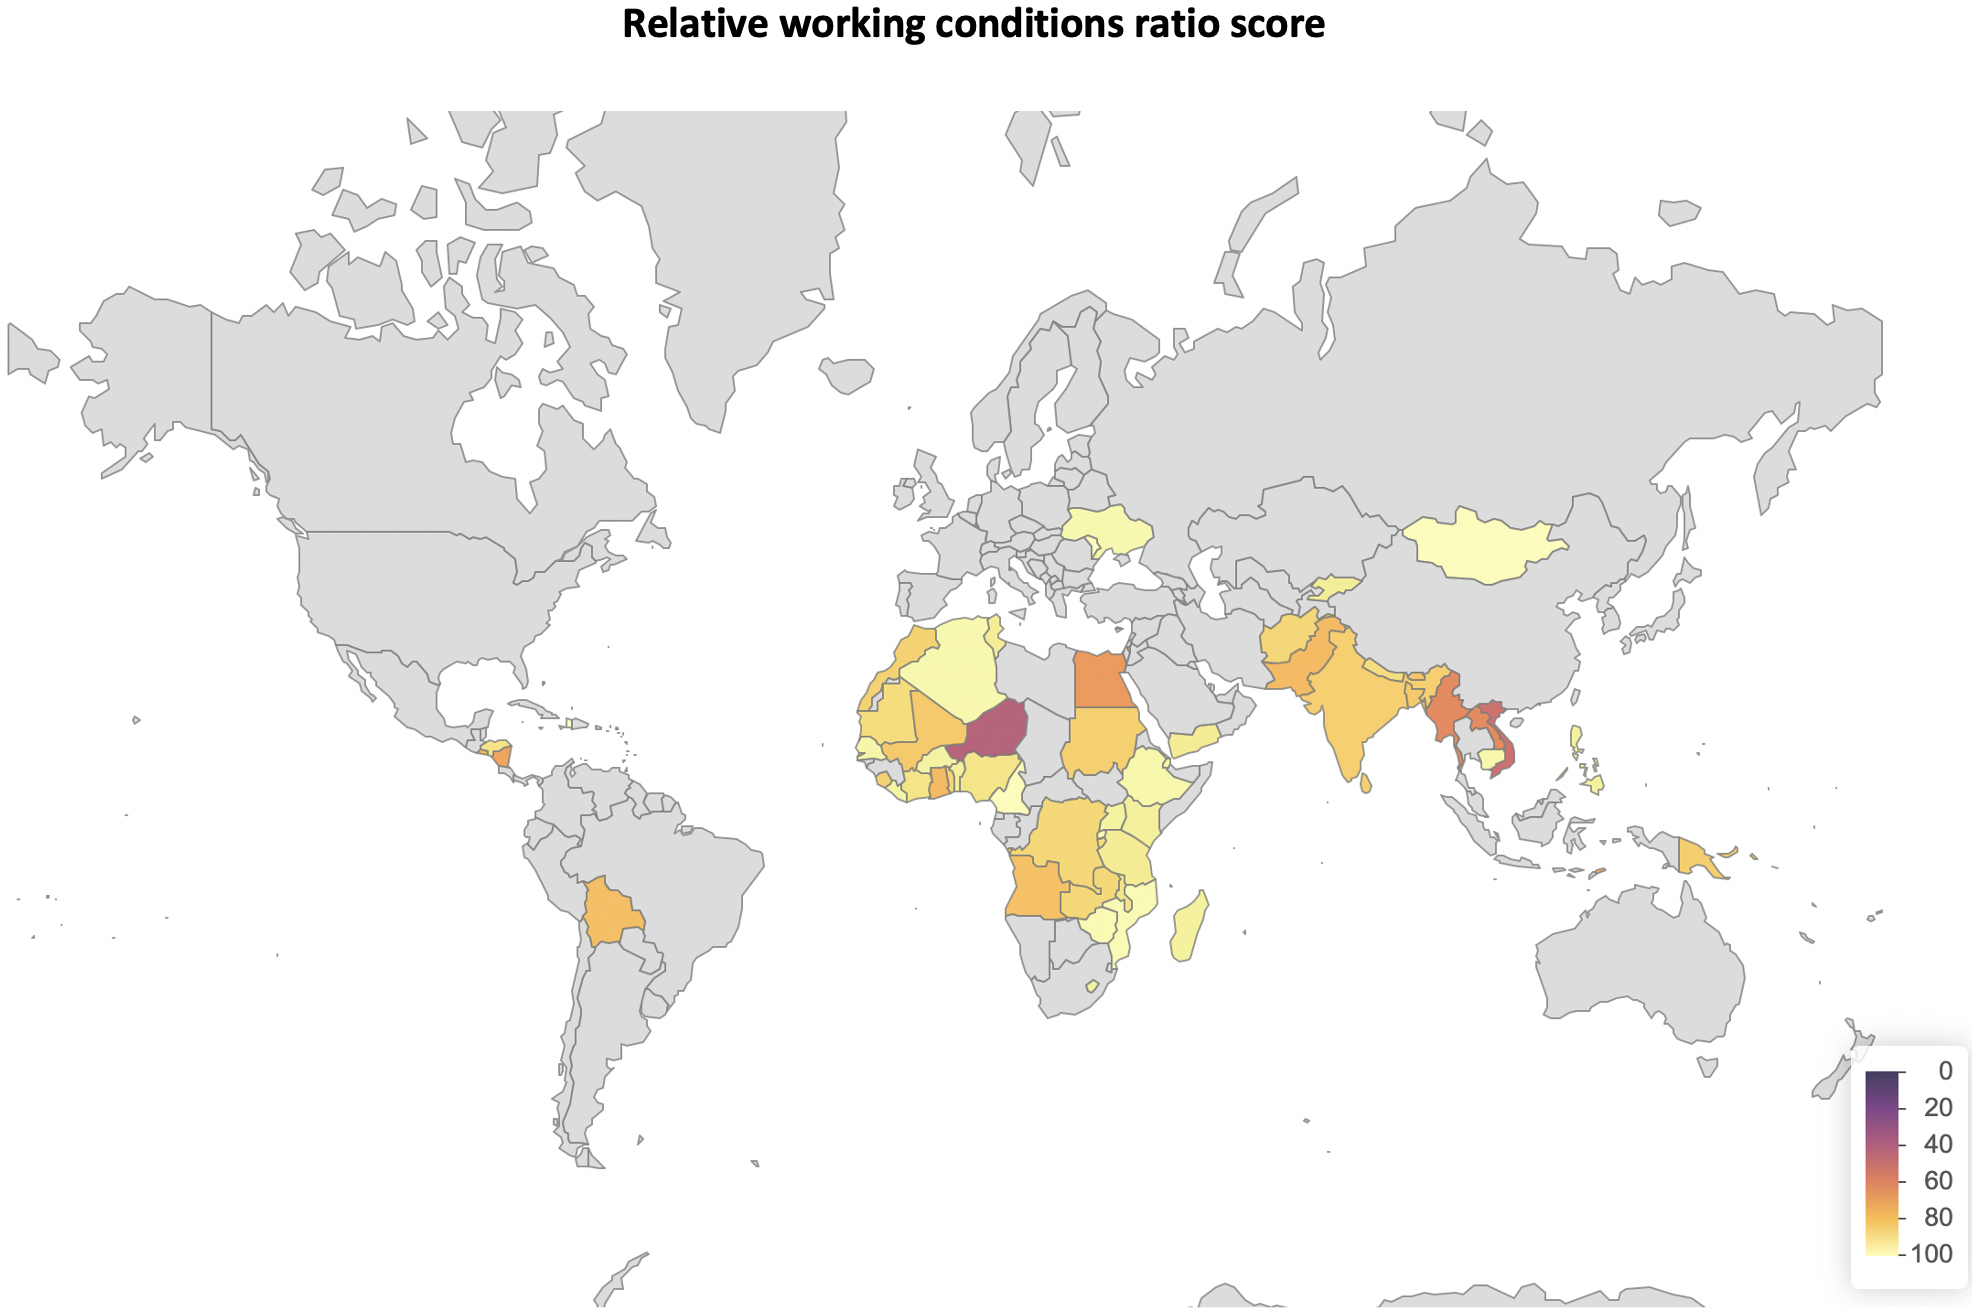
\includegraphics[width=0.7\linewidth,]{figures/maps/wcratio_total} 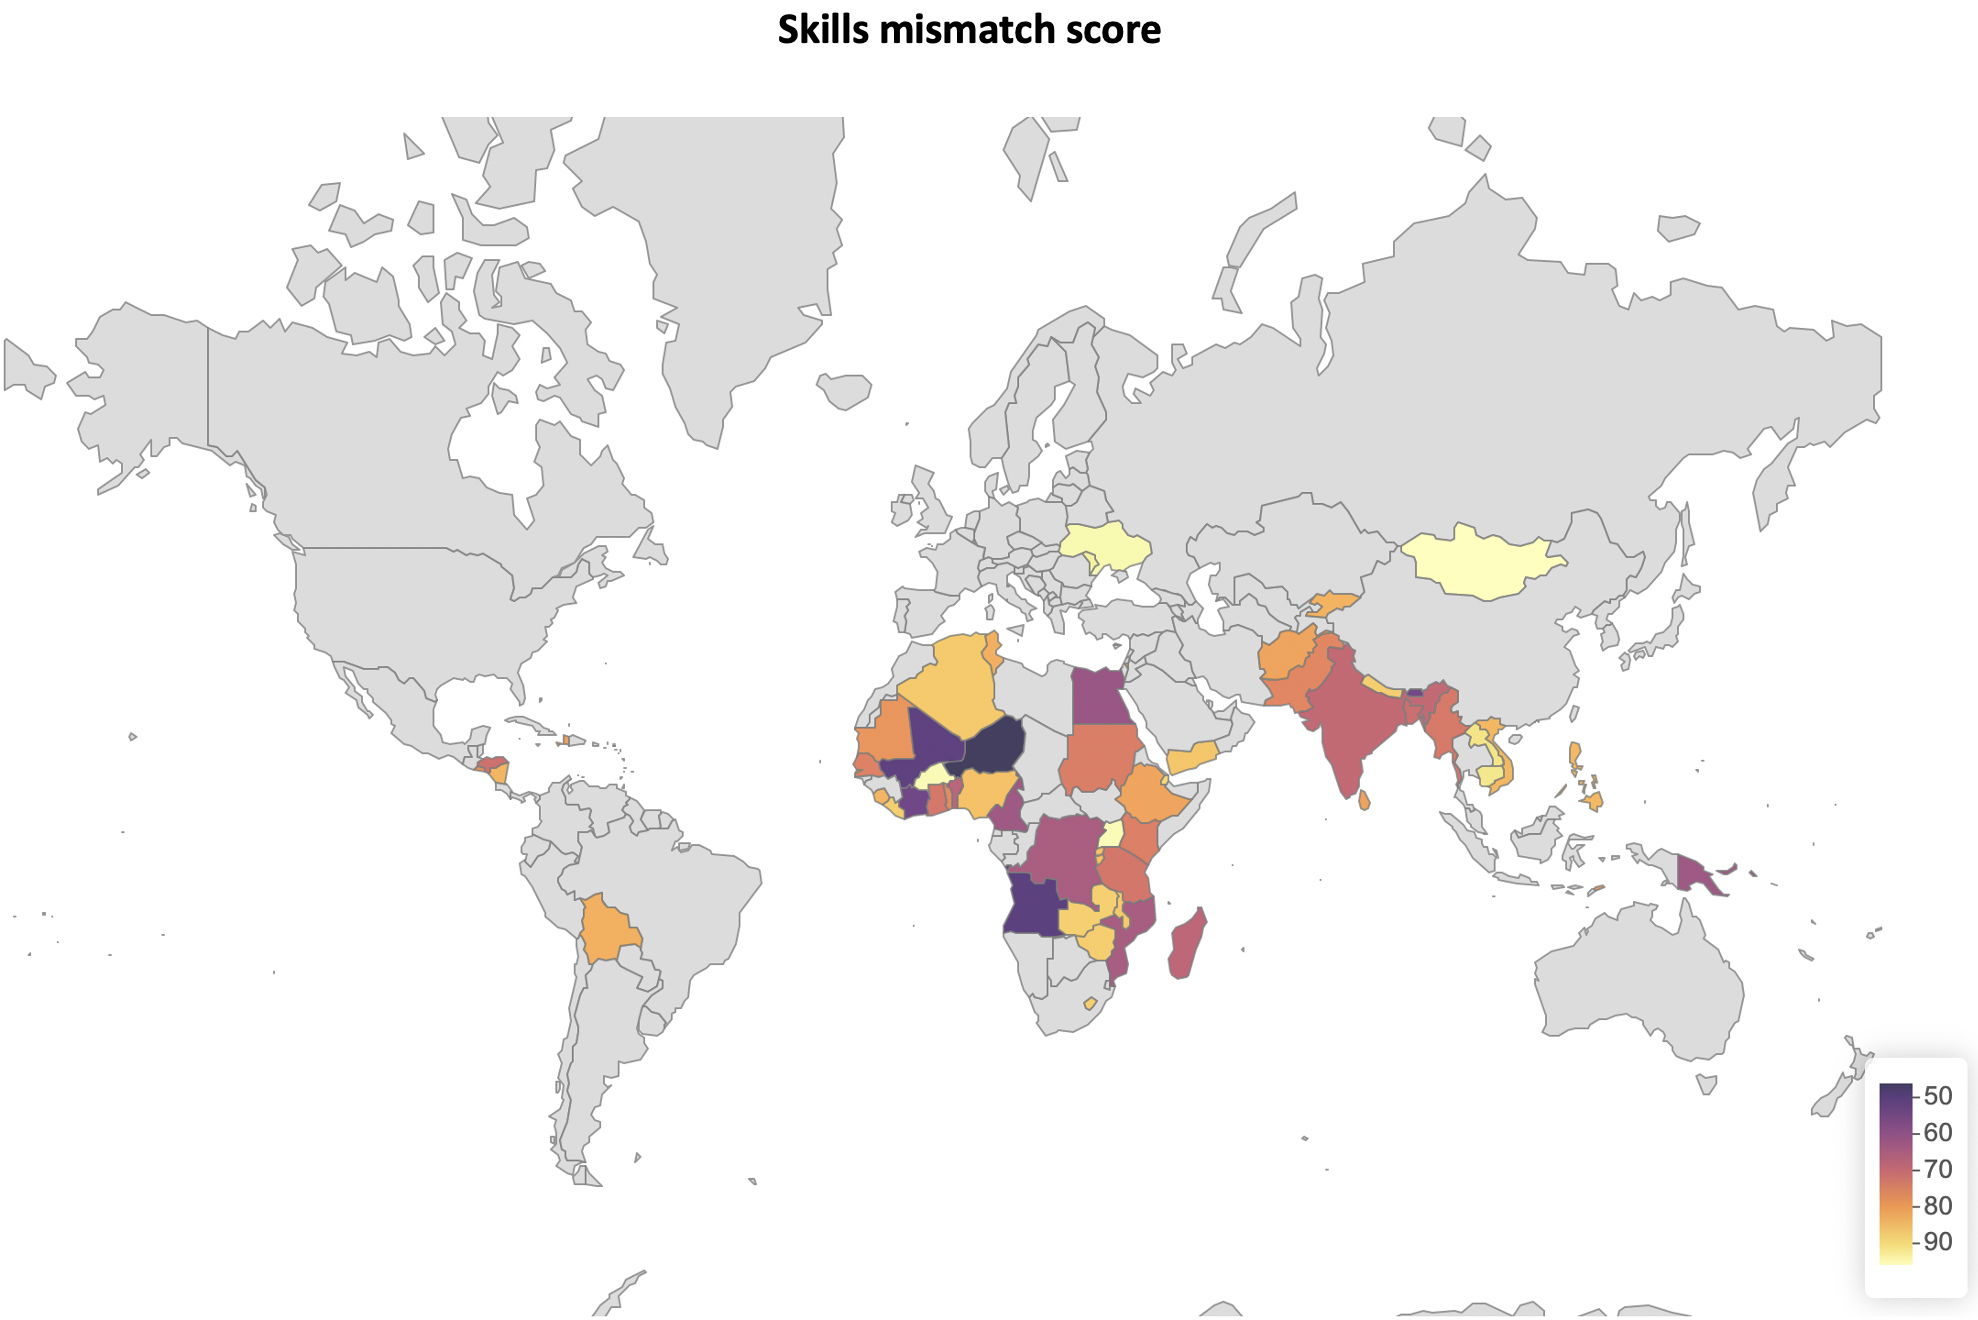
\includegraphics[width=0.7\linewidth,]{figures/maps/skillsmismatch_total} 

}

\caption{Indicators of the transition dimension depicted by country}\label{fig:fig-transitionmap}
\end{figure}

\begin{figure}[H]

{\centering 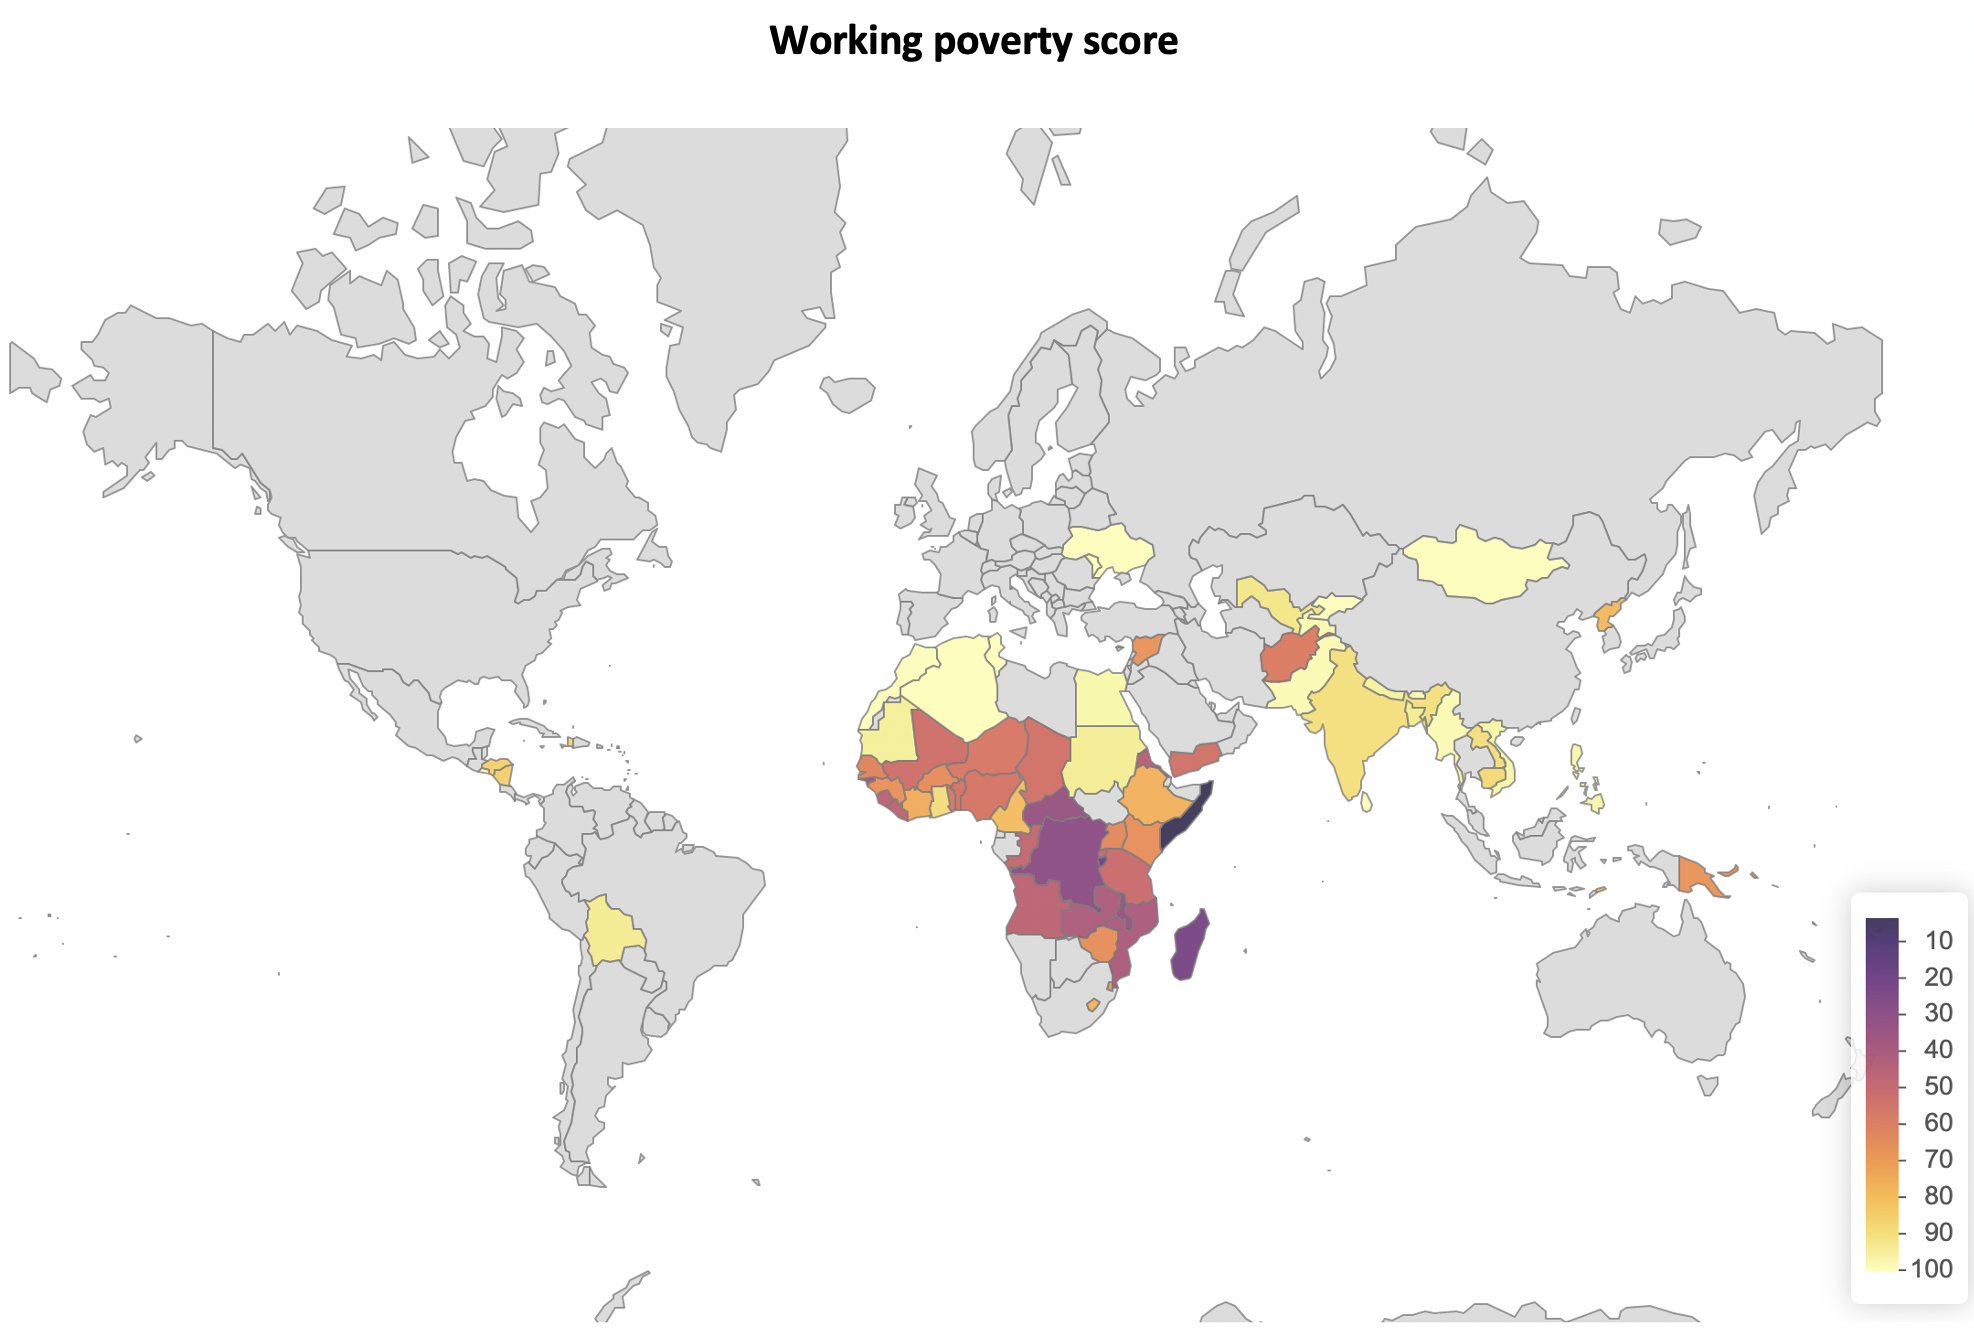
\includegraphics[width=0.52\linewidth,]{figures/maps/workingpoverty_total} 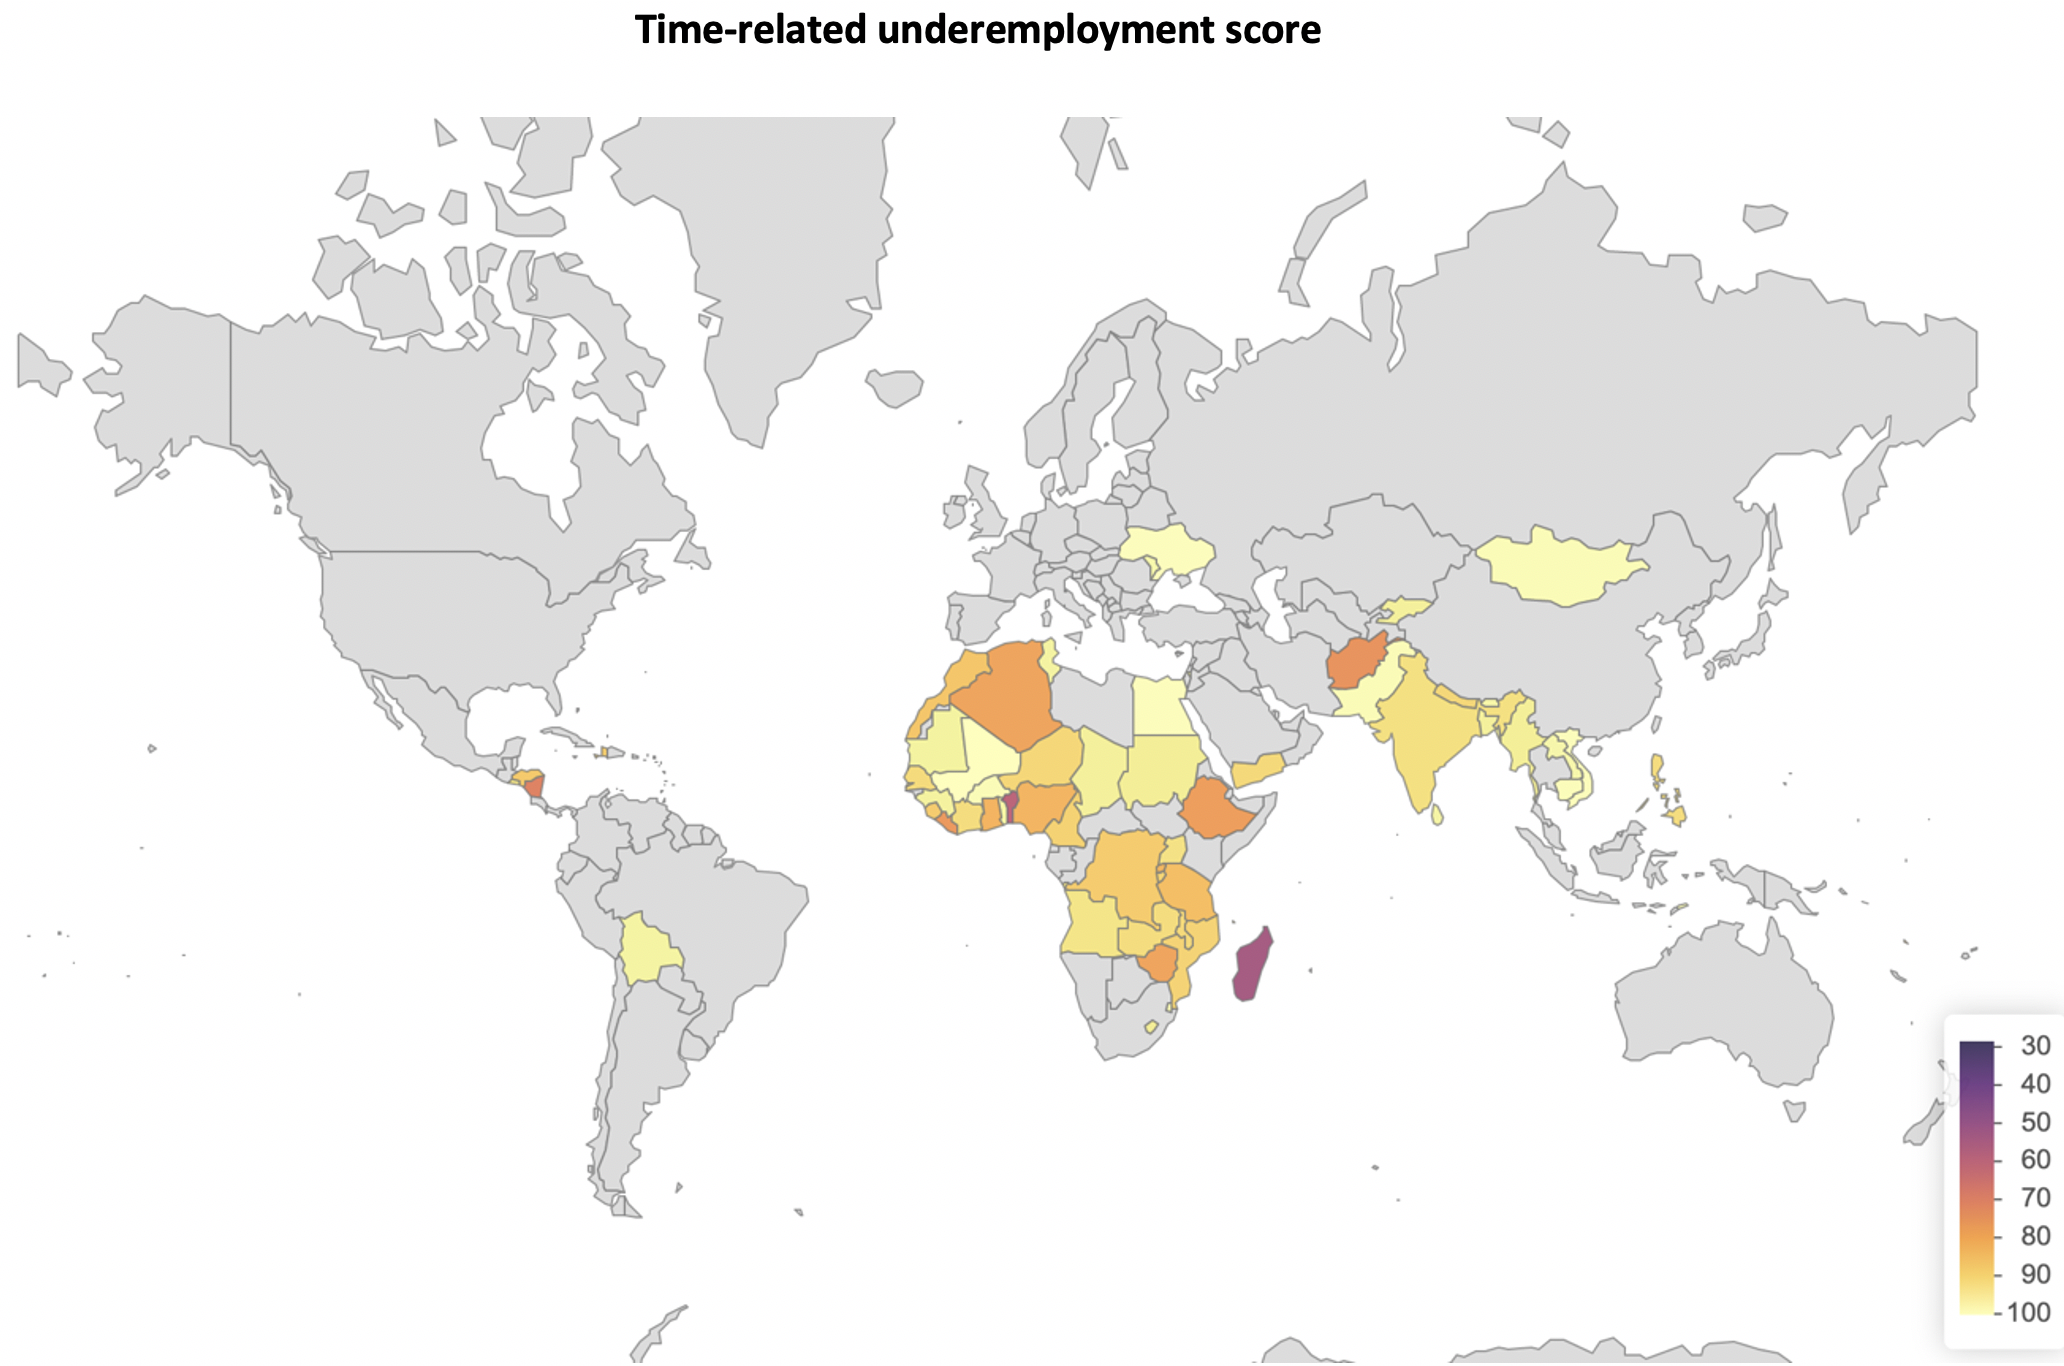
\includegraphics[width=0.52\linewidth,]{figures/maps/underemployment_total} 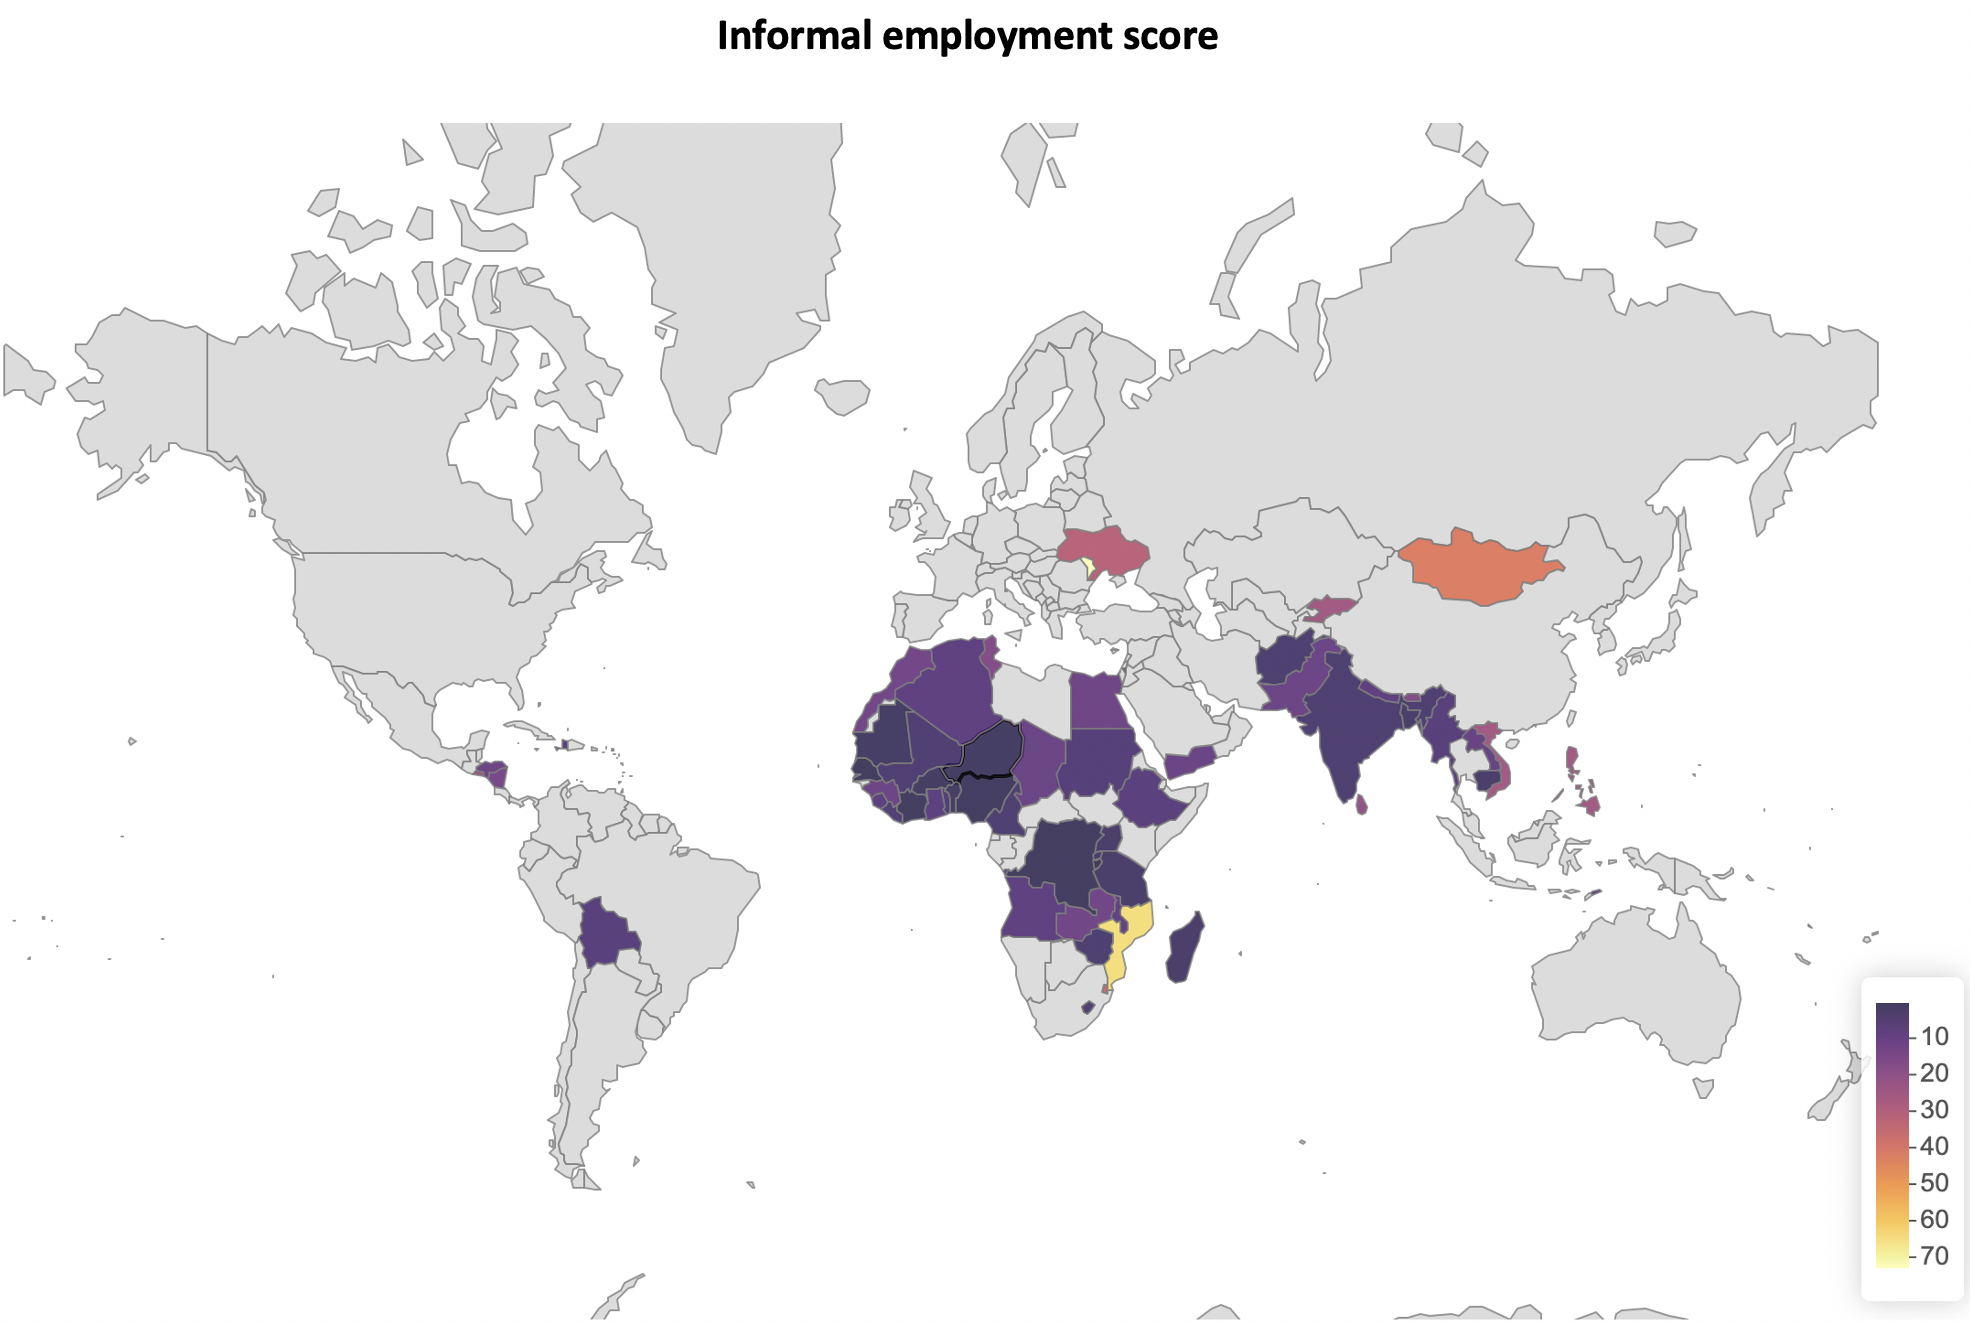
\includegraphics[width=0.52\linewidth,]{figures/maps/informal_total} 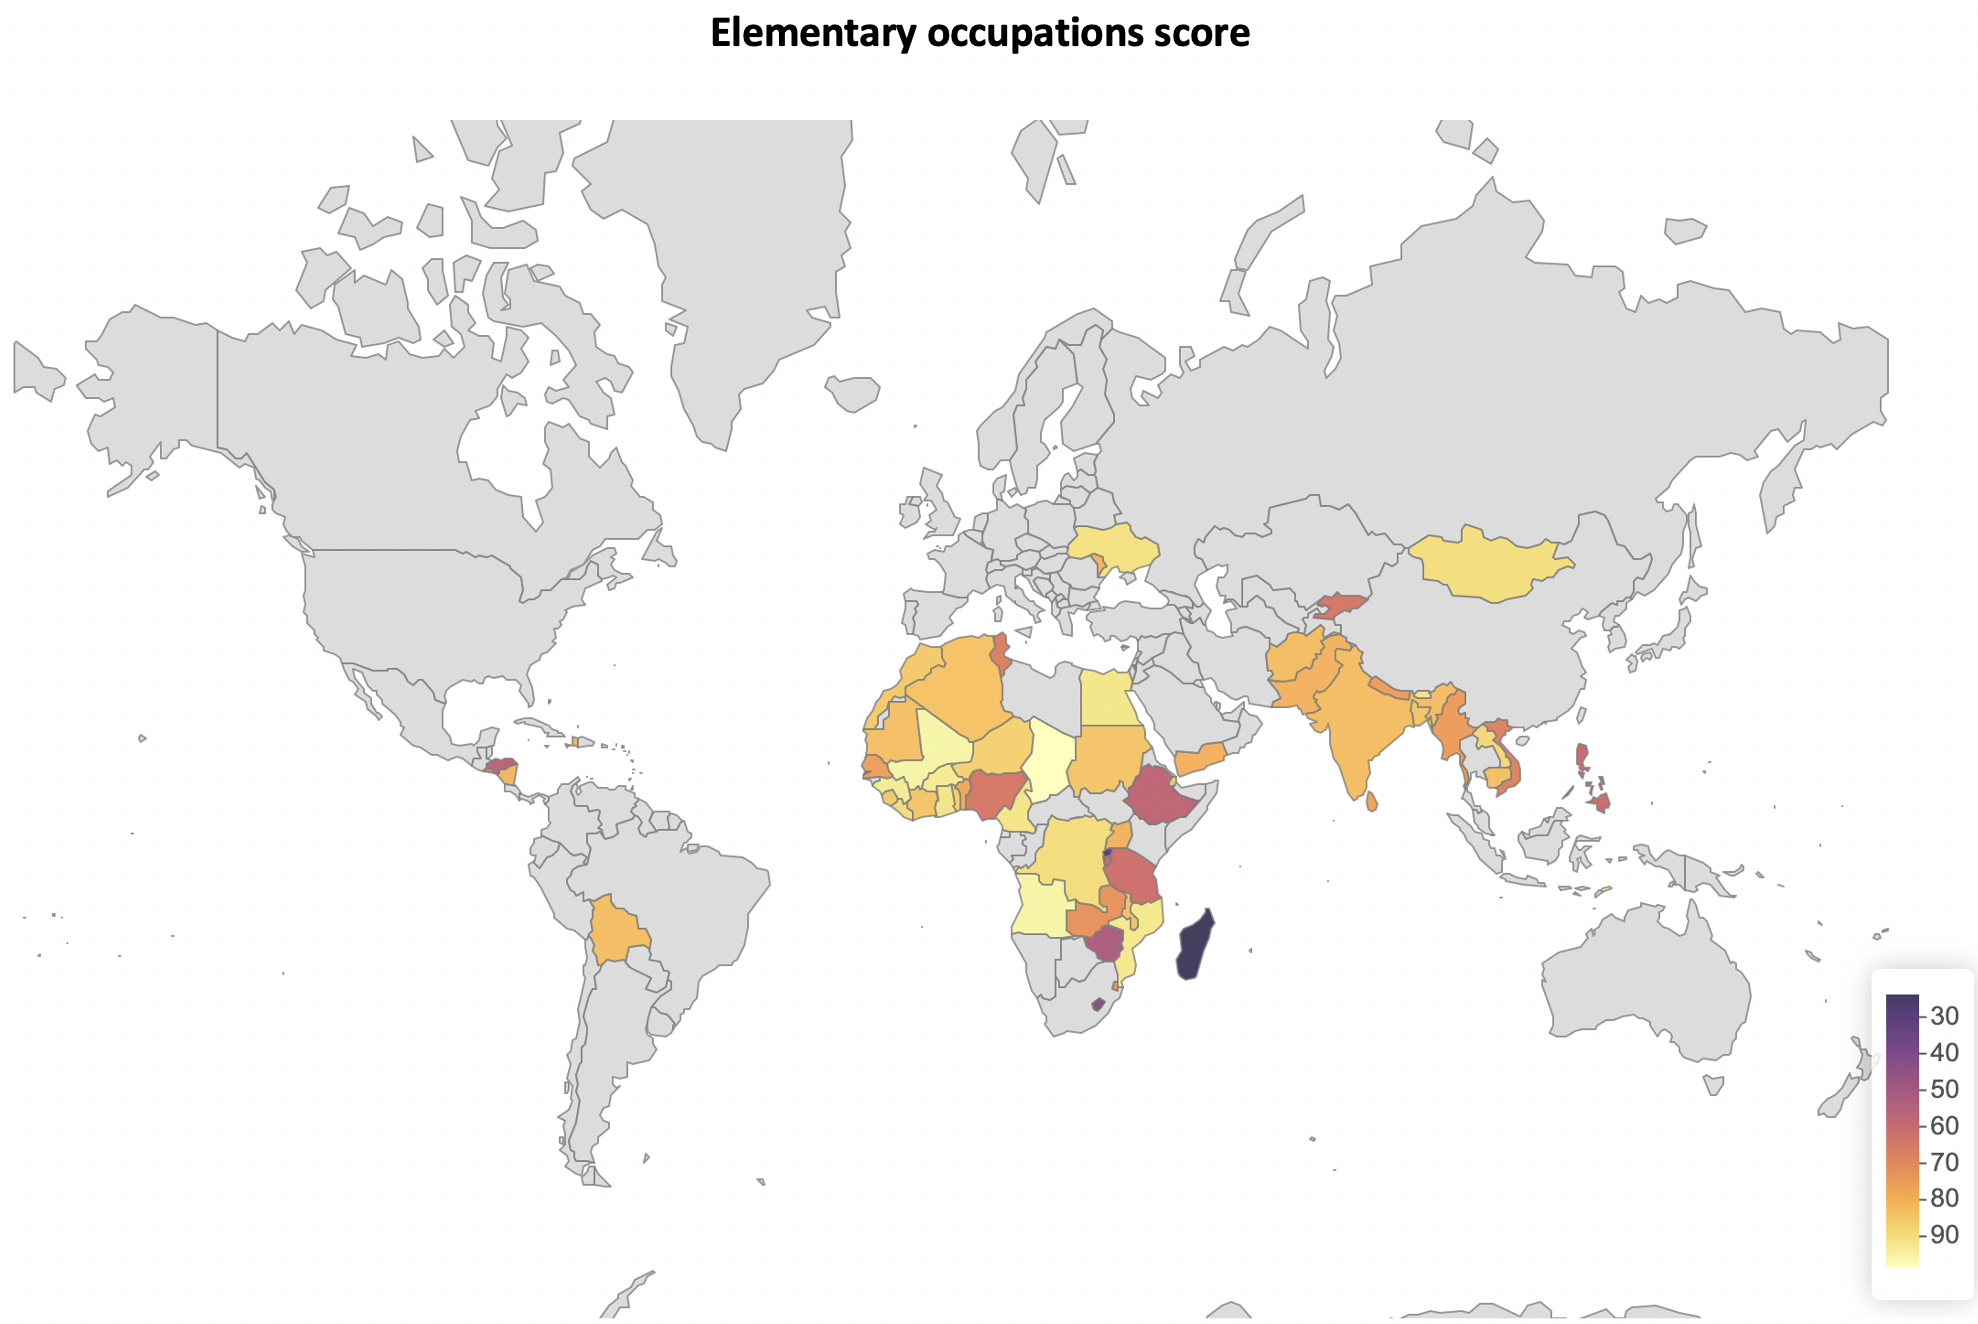
\includegraphics[width=0.52\linewidth,]{figures/maps/elementaryoccup_total} 

}

\caption{Indicators of the working conditions dimension depicted by country}\label{fig:fig-workcondmap}
\end{figure}

\begin{figure}[H]

{\centering 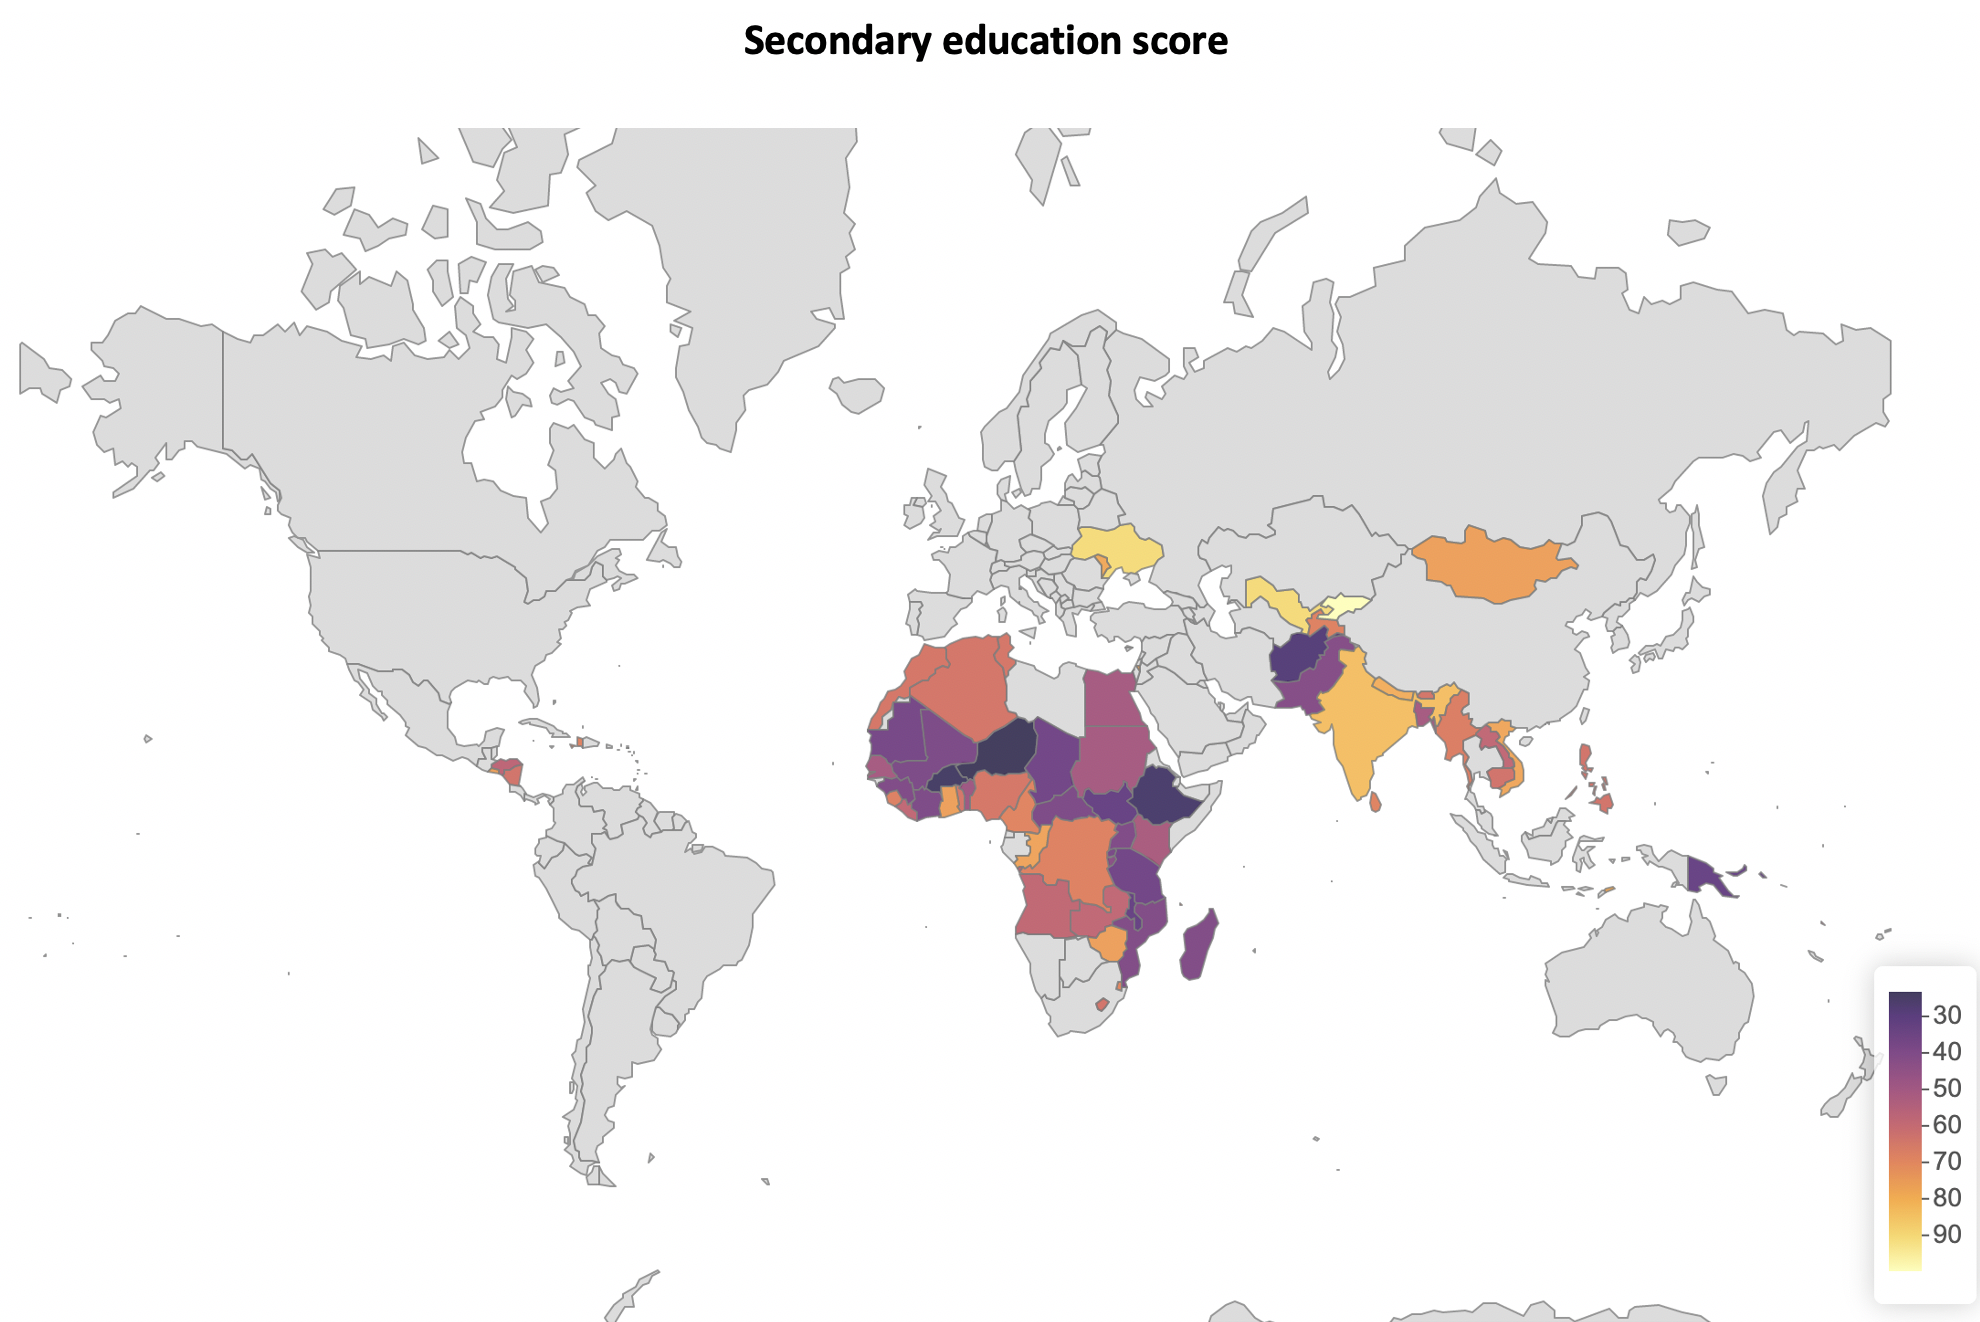
\includegraphics[width=0.69\linewidth,]{figures/maps/secondaryeduc_total} 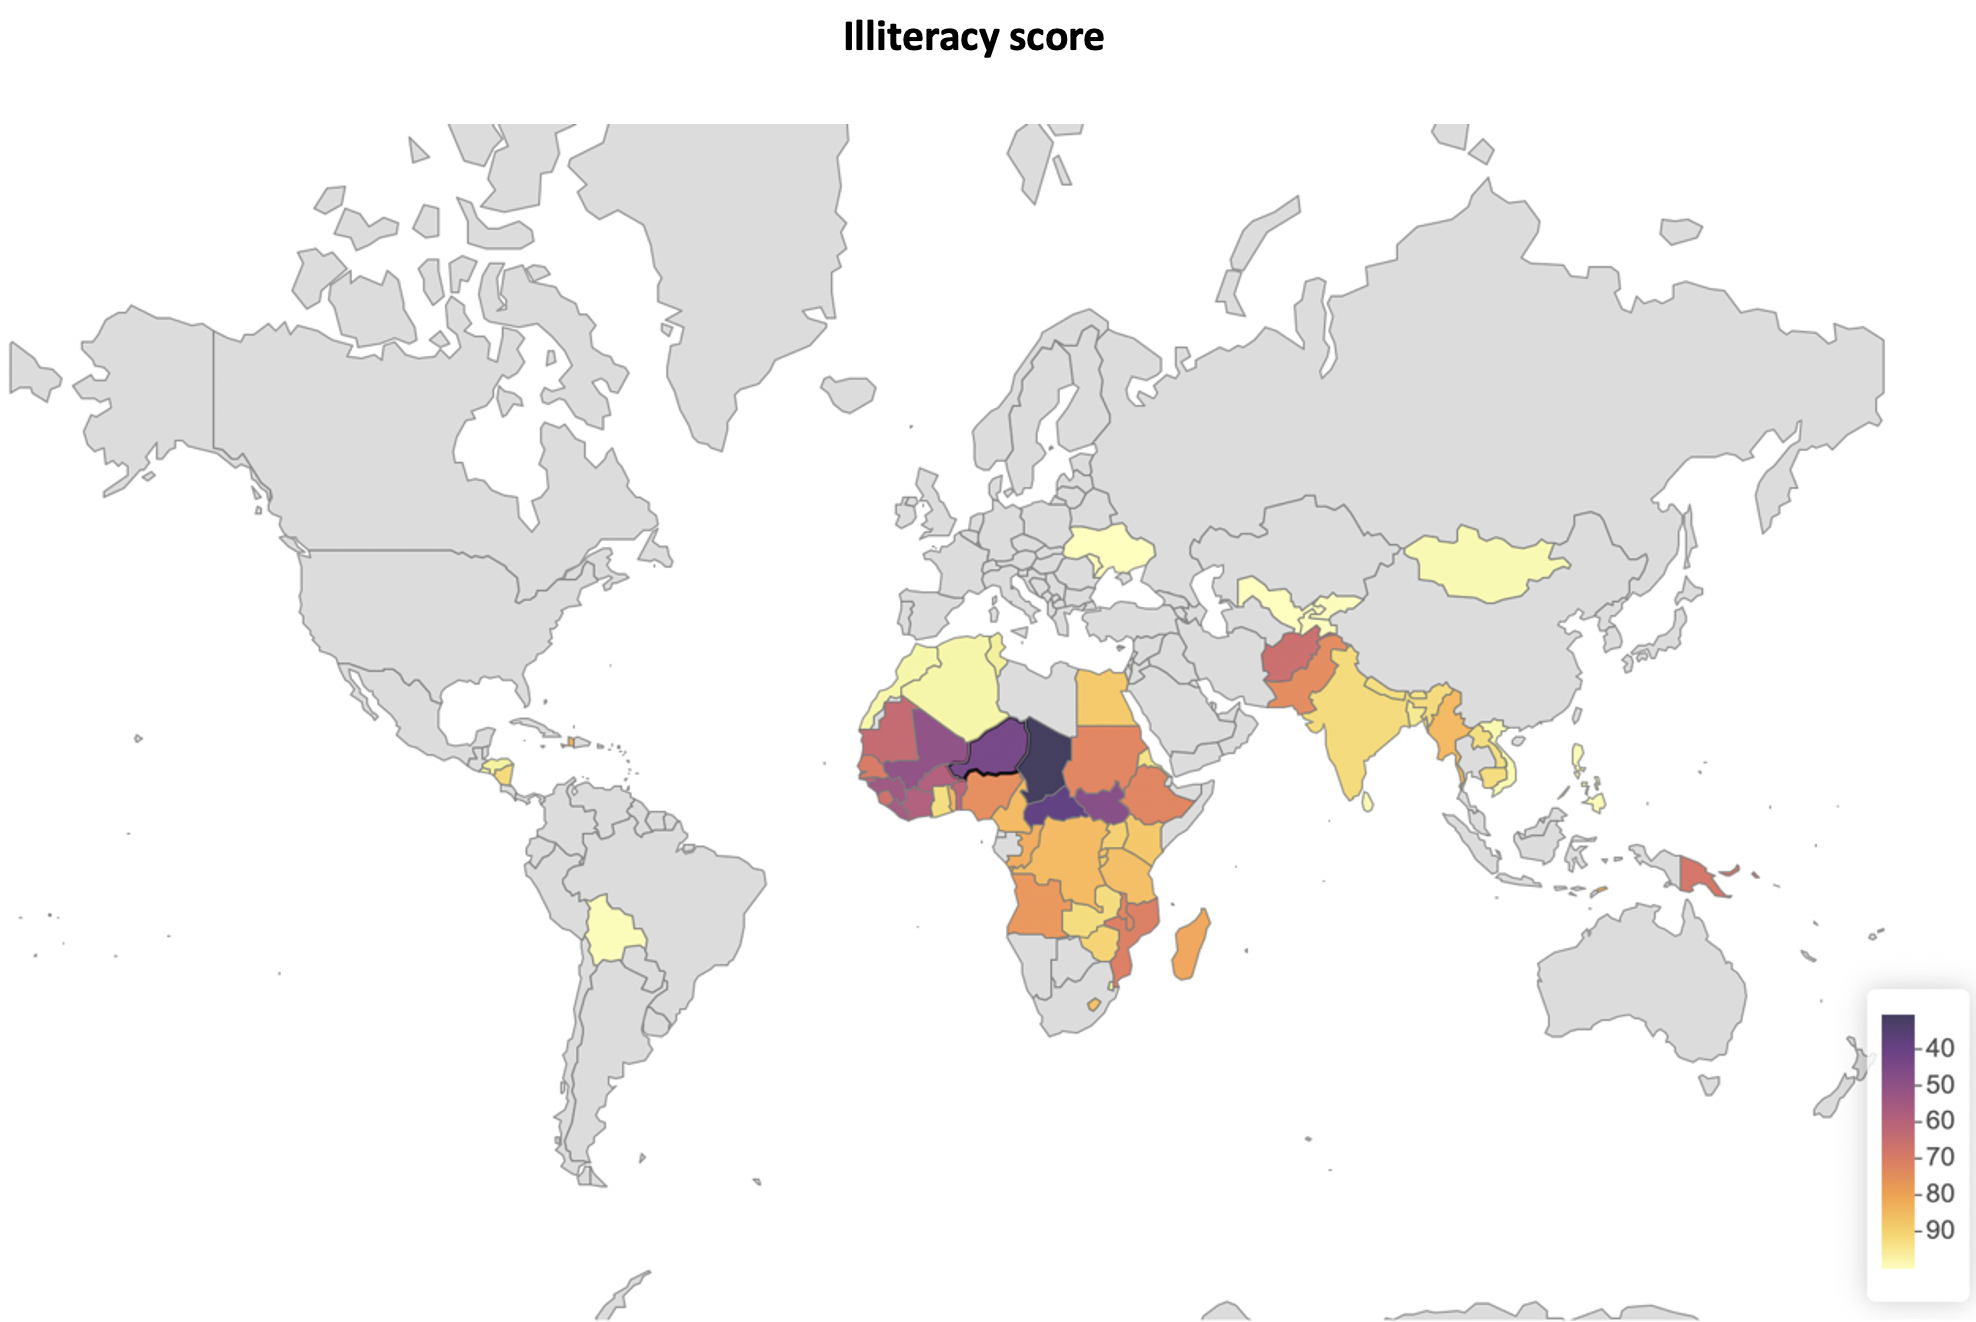
\includegraphics[width=0.69\linewidth,]{figures/maps/illiteracy_total} 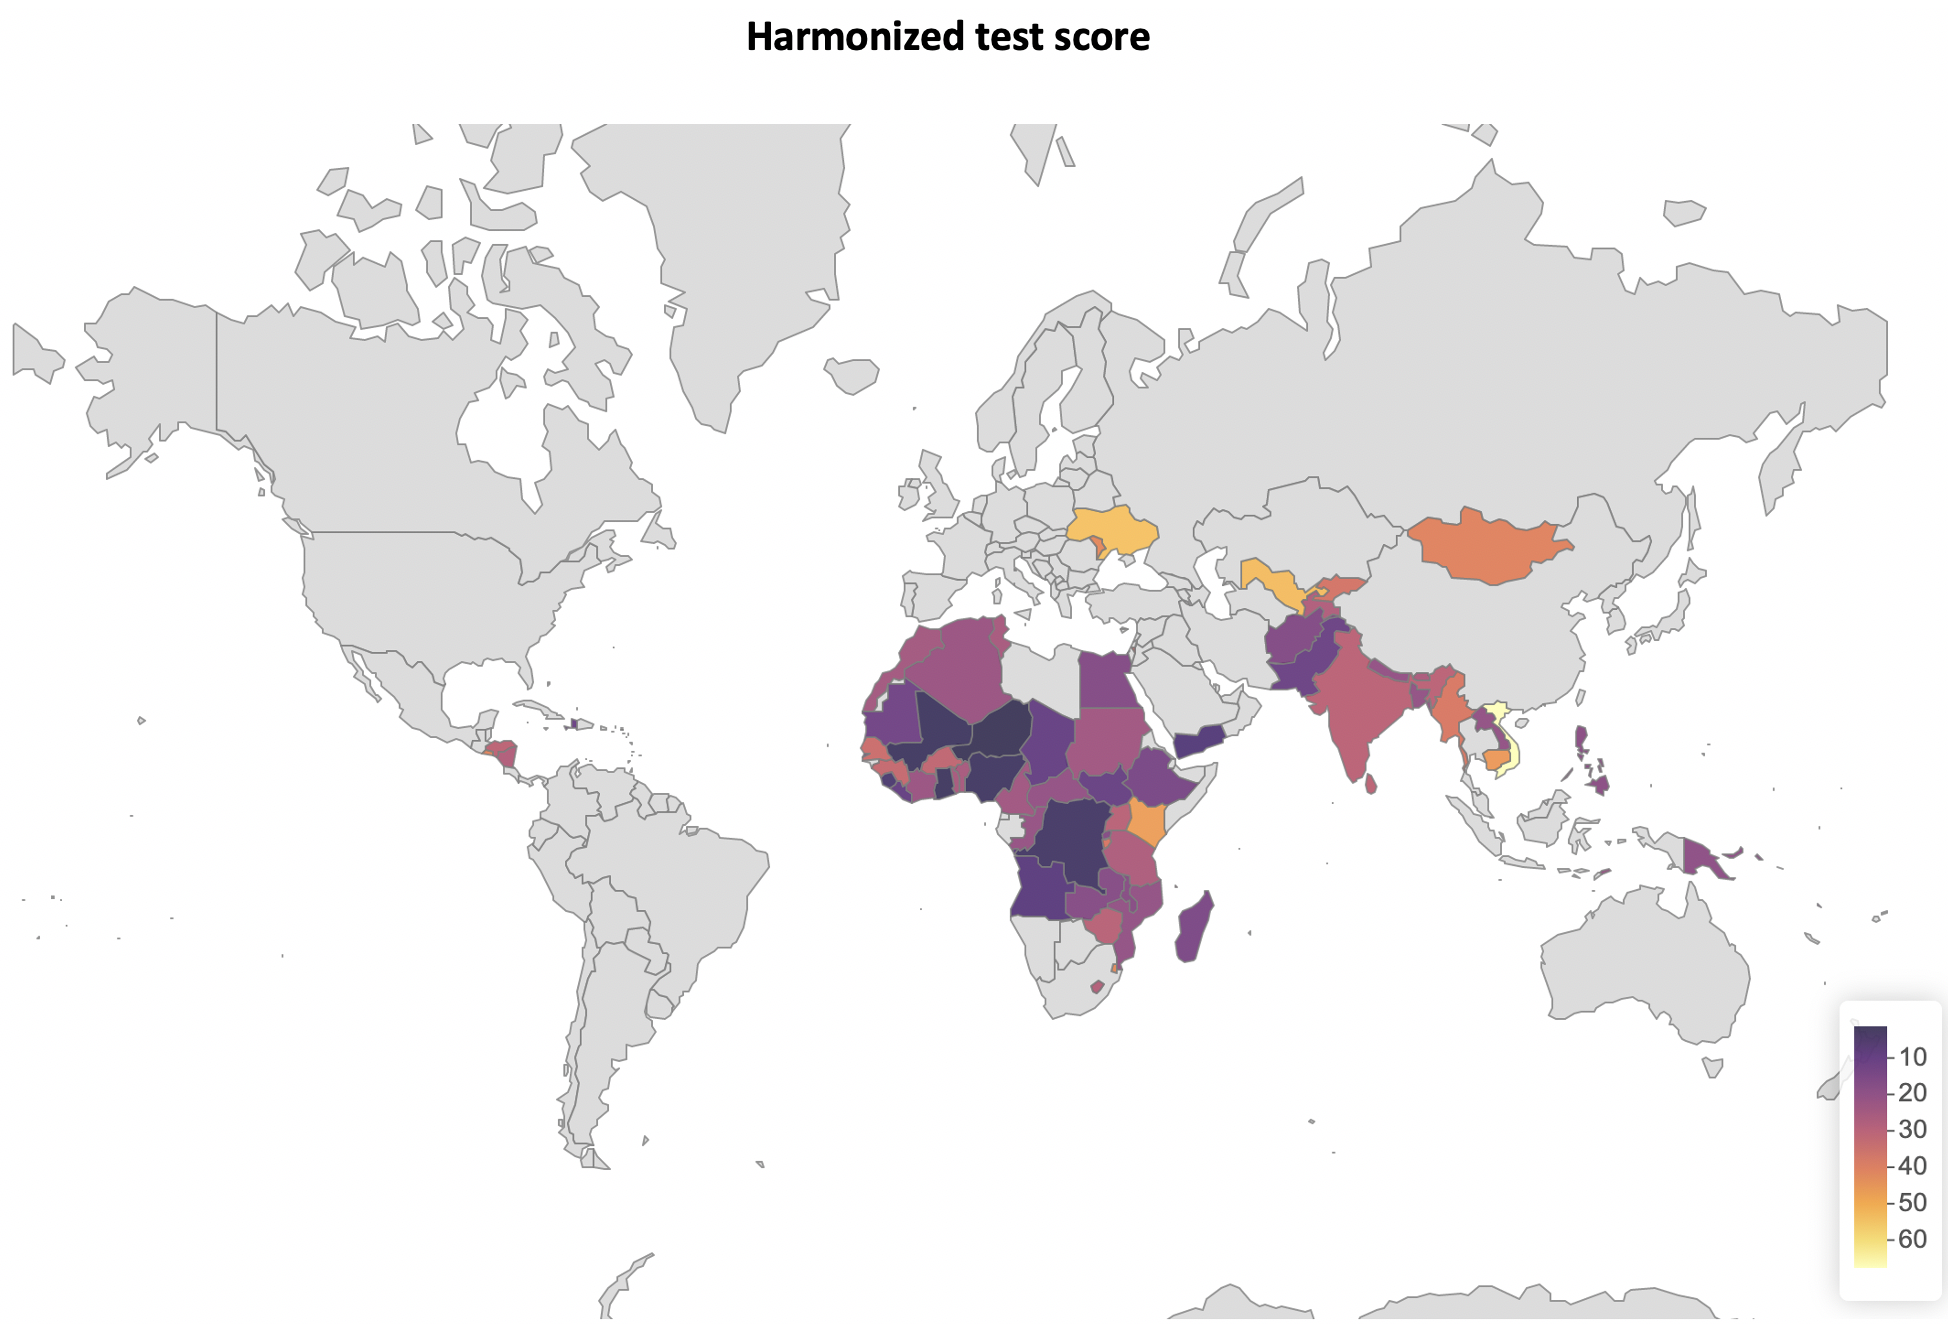
\includegraphics[width=0.69\linewidth,]{figures/maps/harmonizedtest_total} 

}

\caption{Indicators of the education dimension depicted by country}\label{fig:fig-educationmap}
\end{figure}

\begin{figure}[H]

{\centering 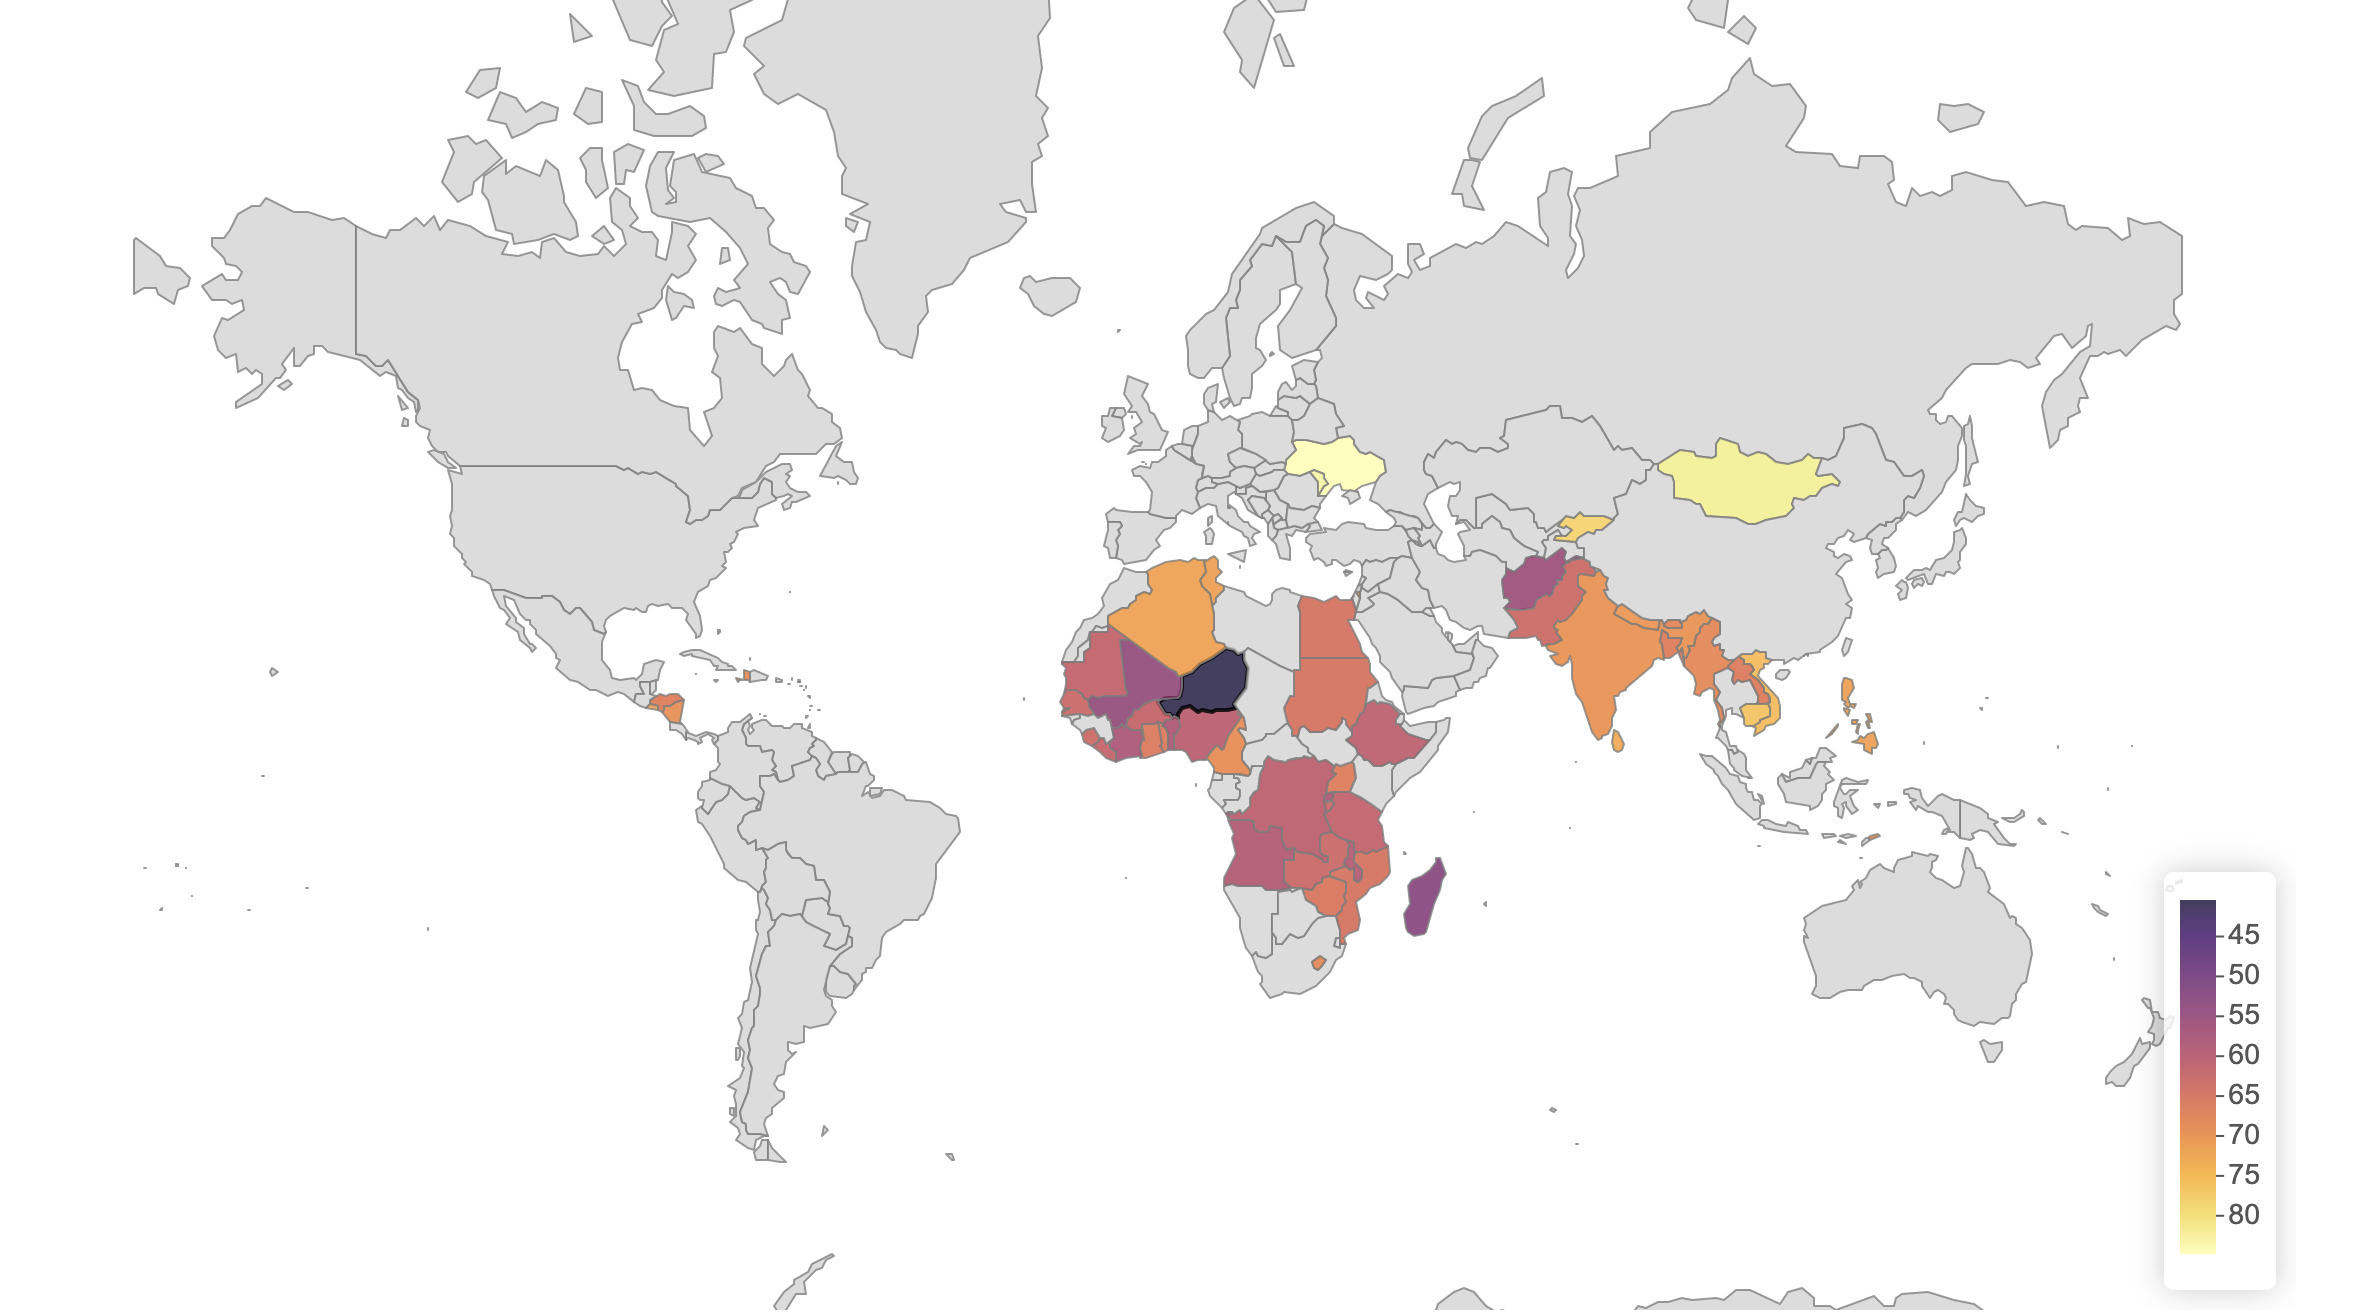
\includegraphics[width=1\linewidth,]{figures/maps/YLILI_total} 

}

\caption{Total YLILI depicted by country}\label{fig:fig-worldmap}
\end{figure}

\begin{figure}[H]

{\centering 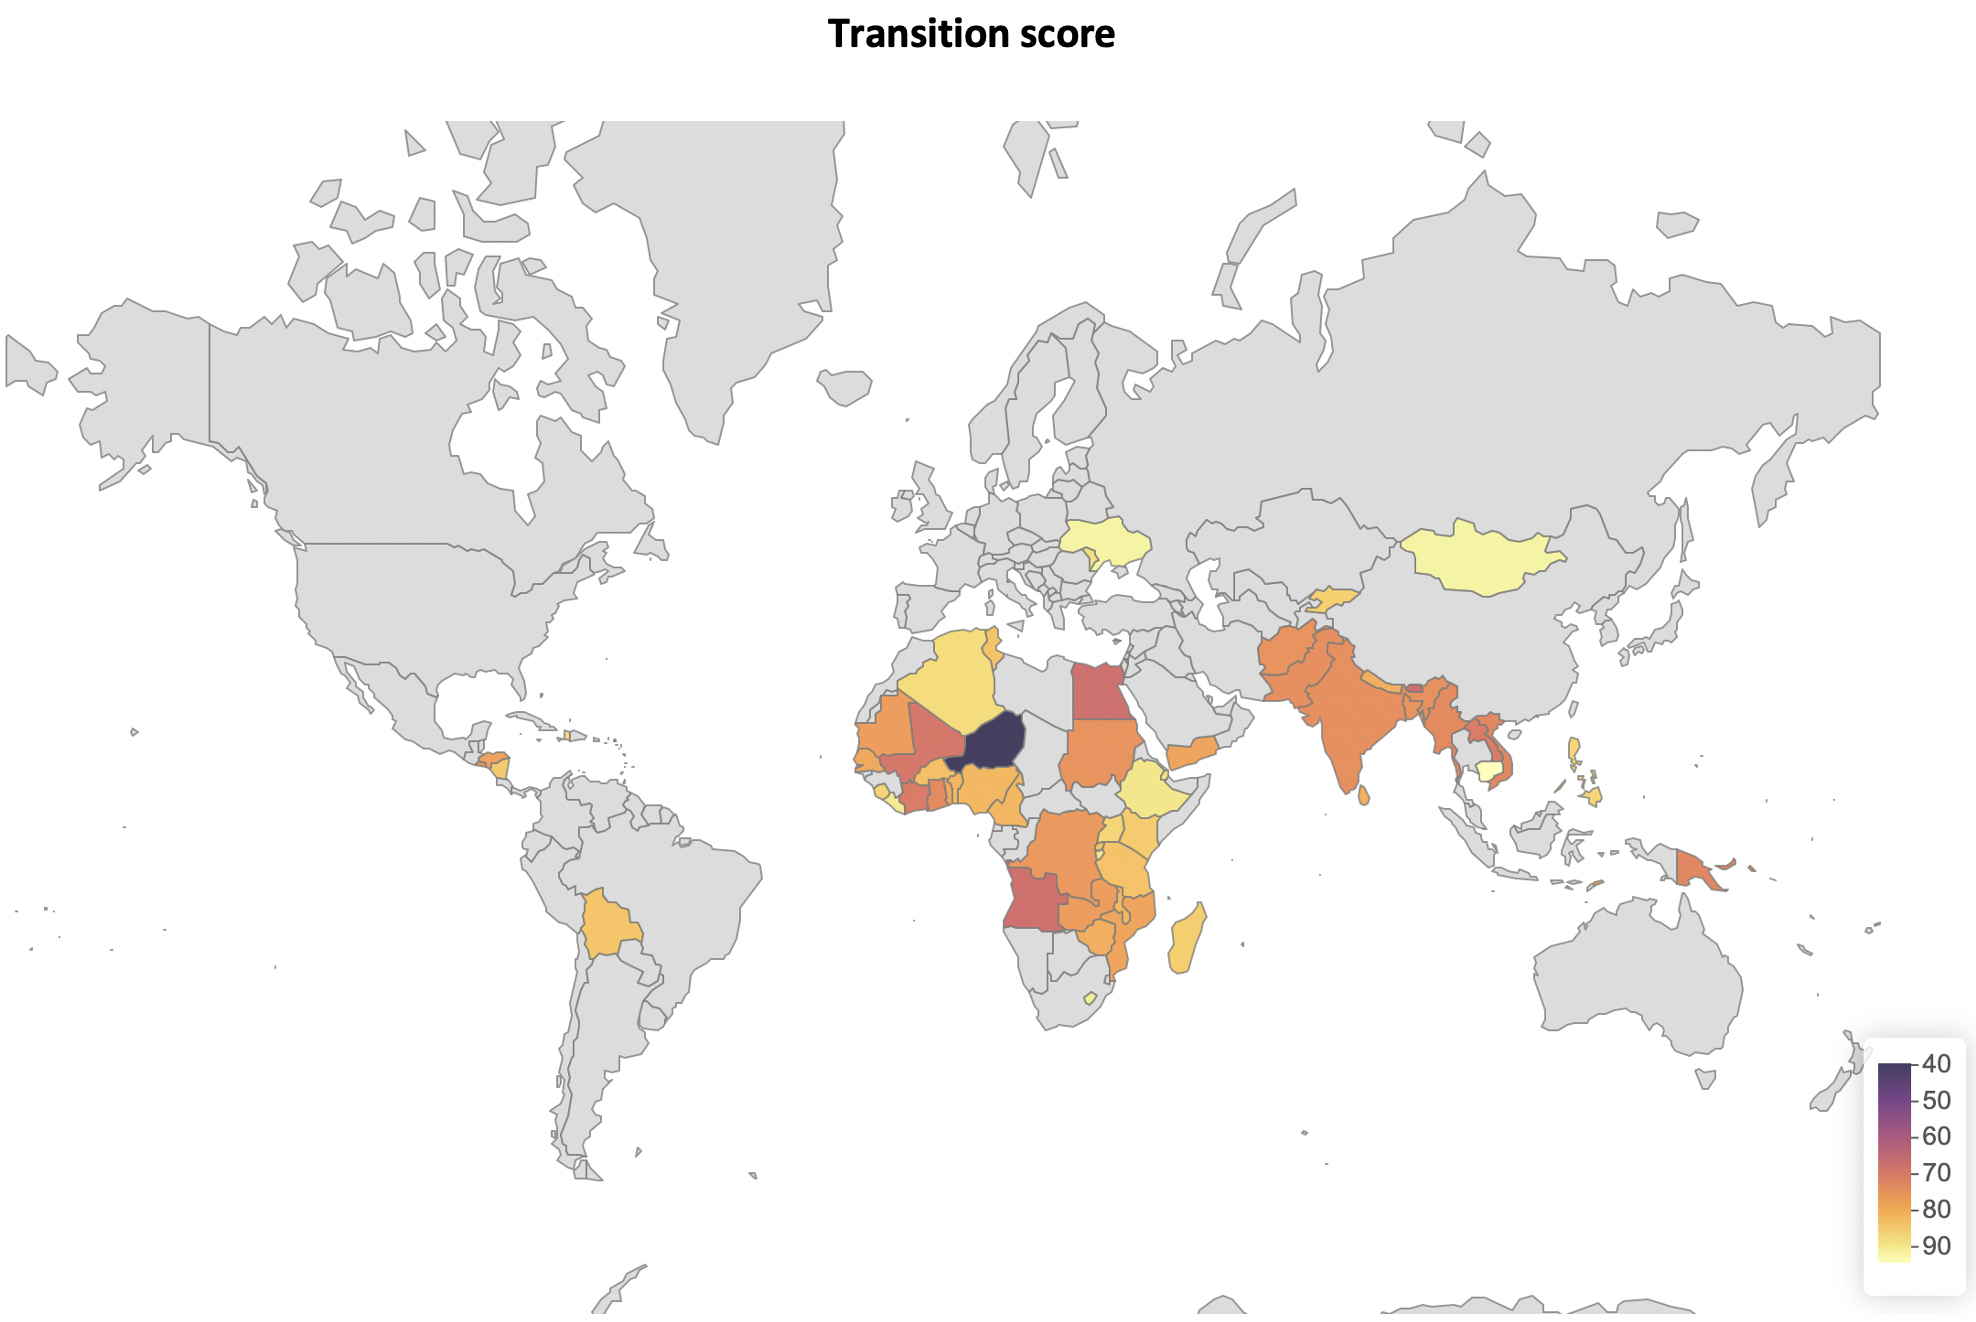
\includegraphics[width=0.69\linewidth,]{figures/maps/transition_total} 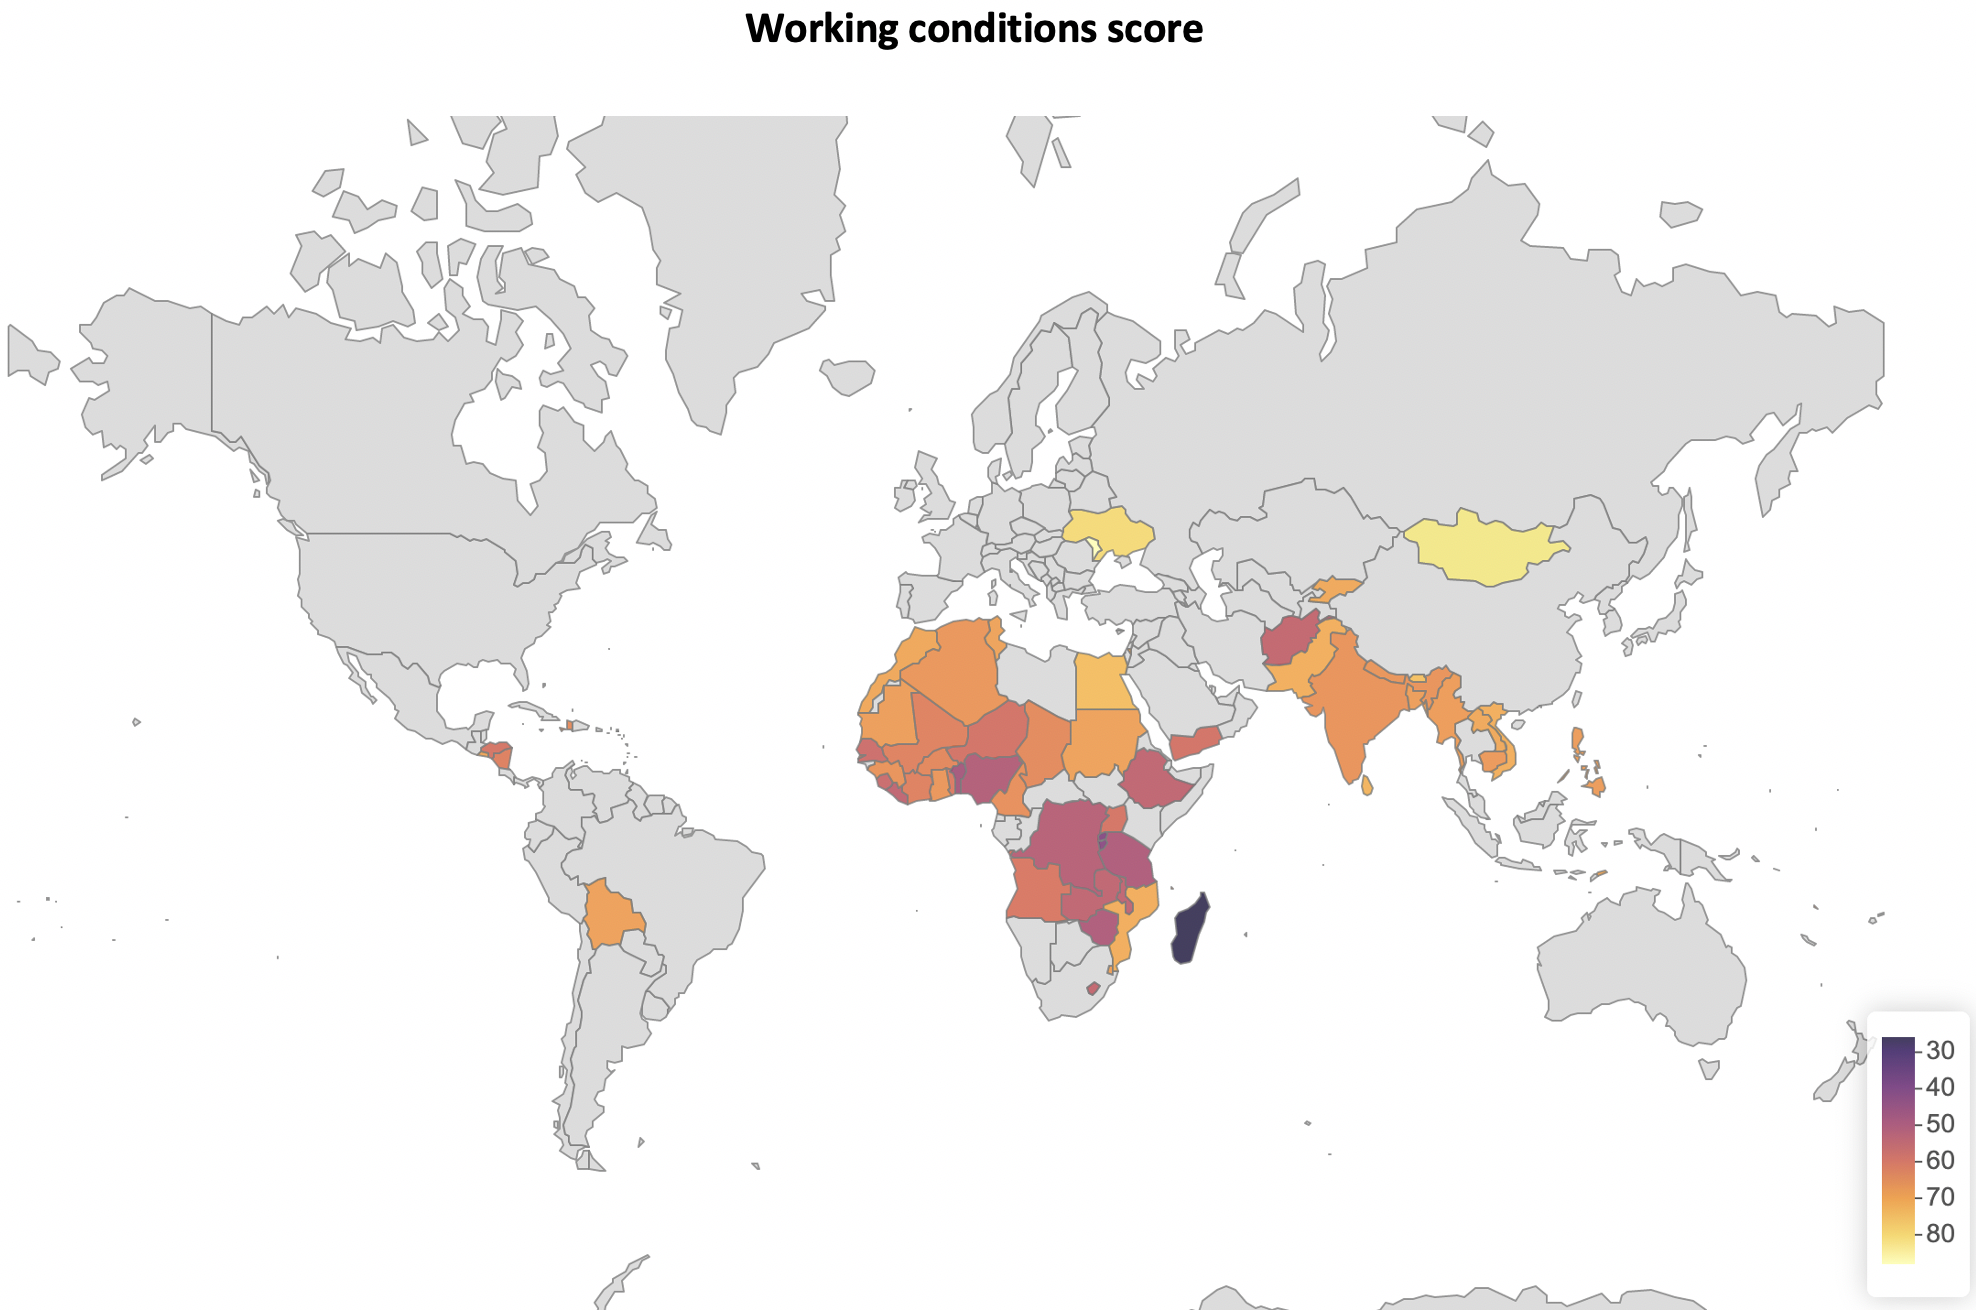
\includegraphics[width=0.69\linewidth,]{figures/maps/working_conditions_total} 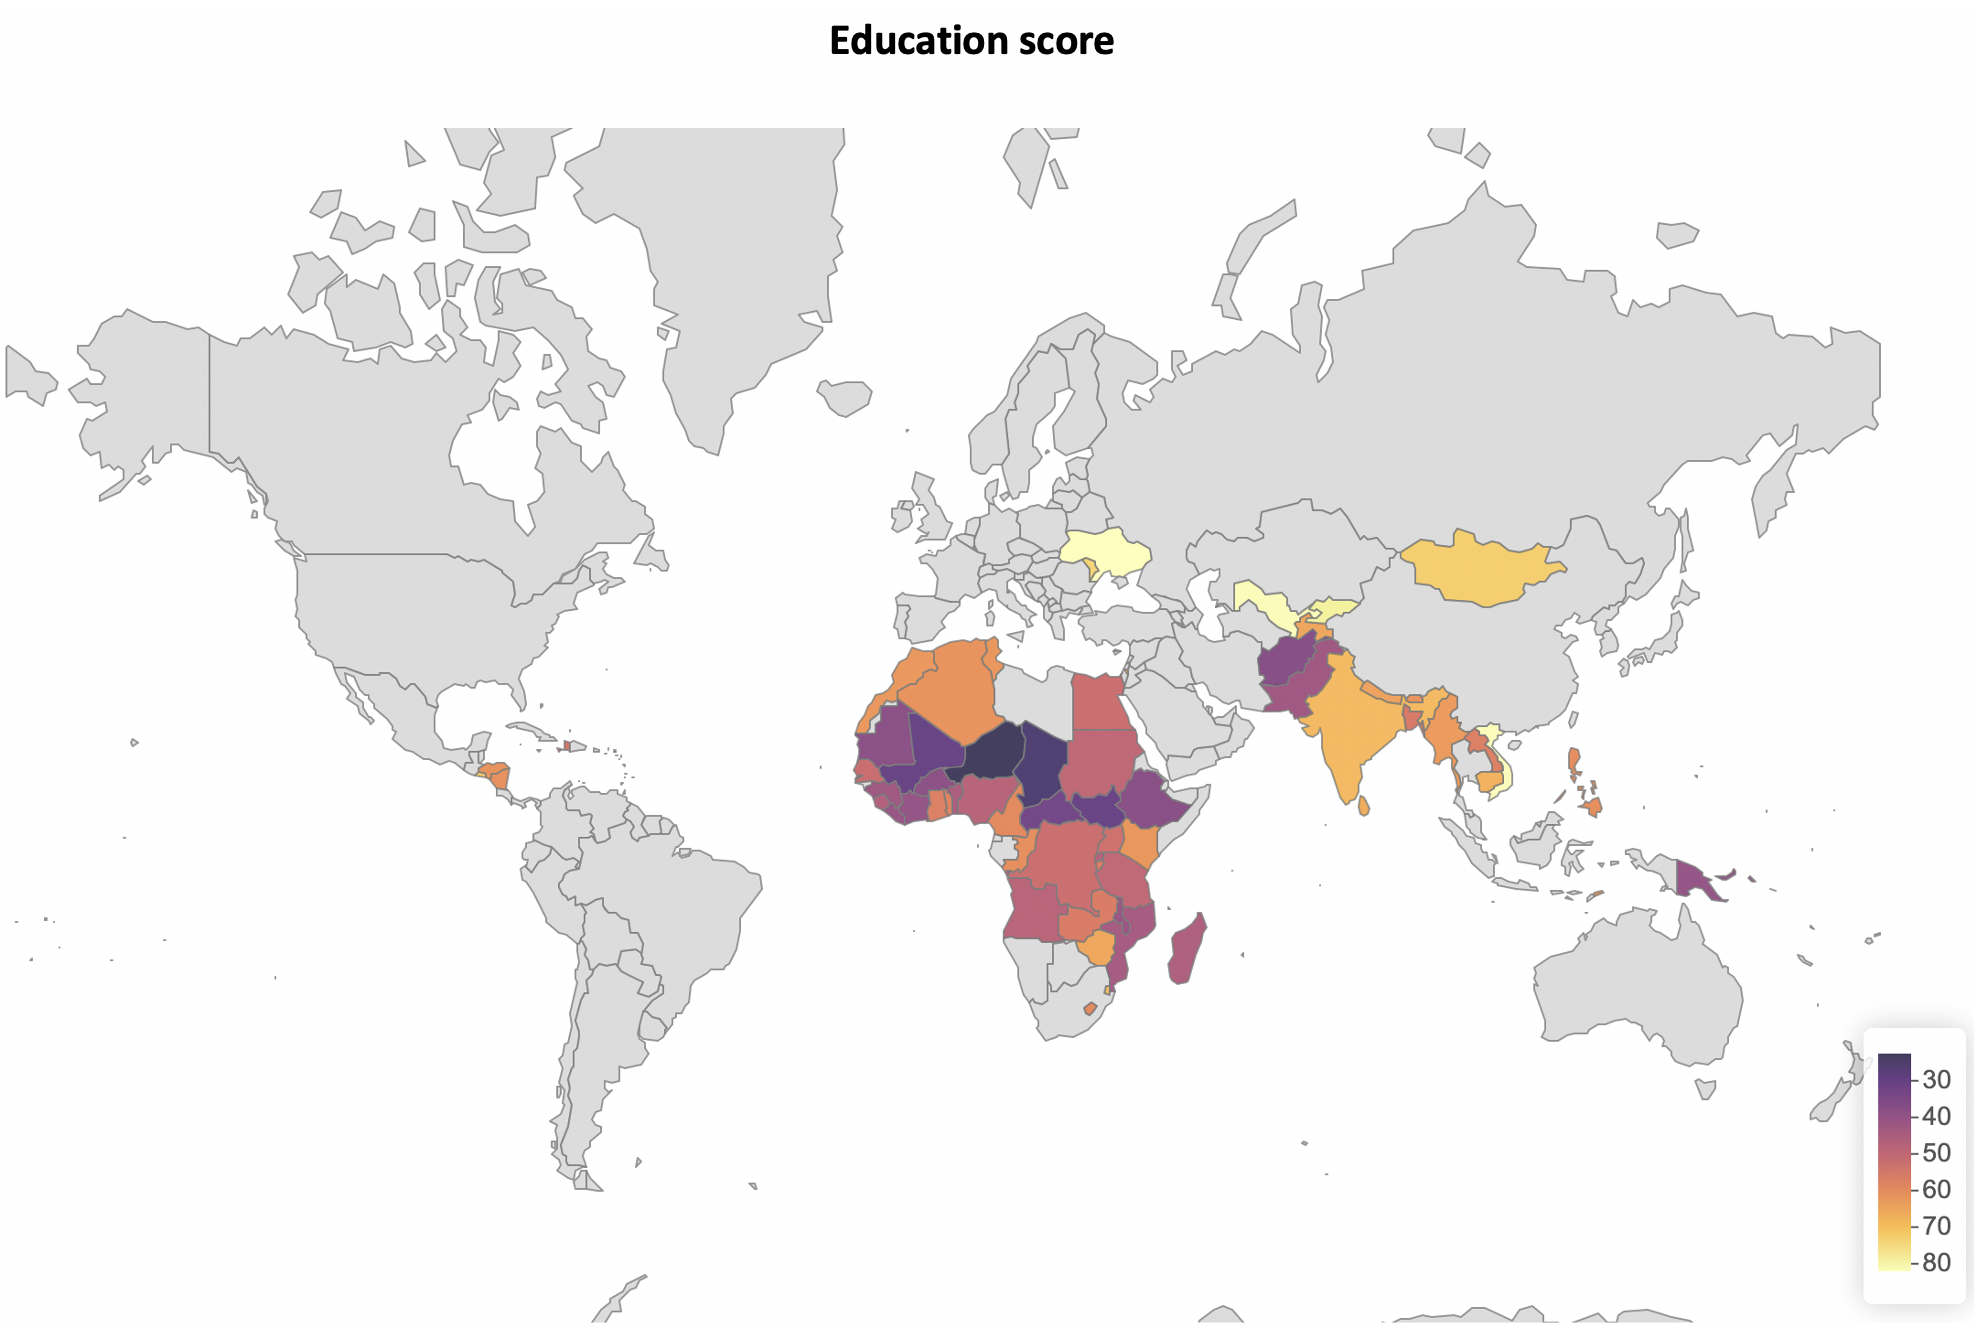
\includegraphics[width=0.69\linewidth,]{figures/maps/education_total} 

}

\caption{Dimensions of the YLILI depicted by country}\label{fig:fig-totalmap}
\end{figure}

\begin{figure}[H]
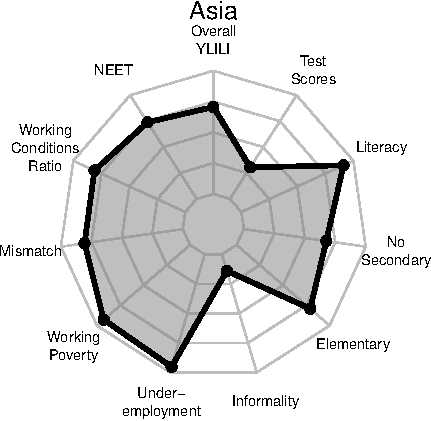
\includegraphics[width=0.49\linewidth,]{figures/fig-spider-1} 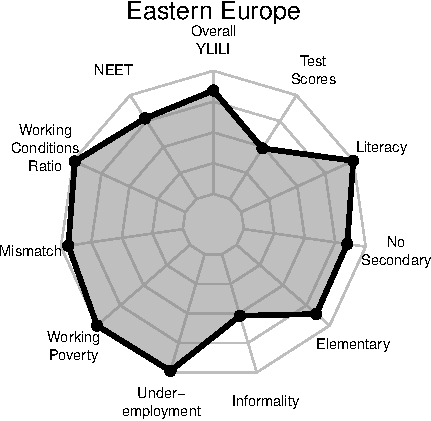
\includegraphics[width=0.49\linewidth,]{figures/fig-spider-2} 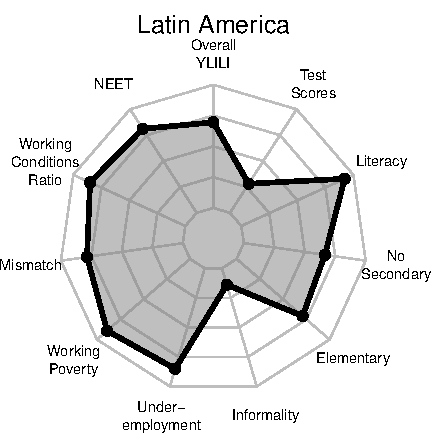
\includegraphics[width=0.49\linewidth,]{figures/fig-spider-3} 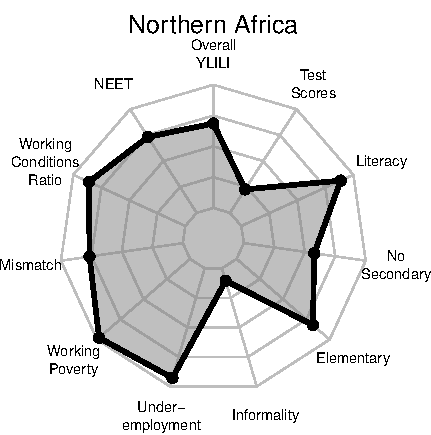
\includegraphics[width=0.49\linewidth,]{figures/fig-spider-4} 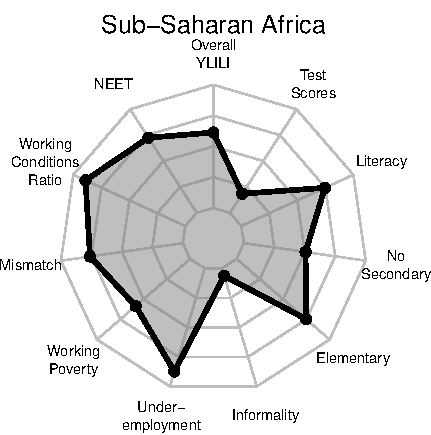
\includegraphics[width=0.49\linewidth,]{figures/fig-spider-5} \caption{Spider charts by world region}\label{fig:fig-spider}
\end{figure}

\newpage

\hypertarget{genderylili}{%
\subsection*{The gender YLILI}\label{genderylili}}

\markboth{The gender YLILI}{Appendix B2}

\newpage
\setlength\LTleft{+.8cm}
\footnotesize{
\begin{longtable}{lcccccccccccccc}
\caption{\textrm{\normalfont \small YLILI by country and gender, last available year \label{tab:tbl-gendiff}}} 
\\ \hline \hline 
Country &  & Region & Male & Female & $\Delta$ & \rot{Rank (Male)} & \rot{Rank (Female)} \\ \hline
Ukraine                           & UKR           & EU \& C. Asia      & 87.38             & 85.77               & 1.60               & 1             & 1               \\
Mongolia                          & MNG           & E. Asia \& Pacific & 81.54             & 82.85               & -1.31              & 2             & 2               \\
Kyrgyzstan                        & KGZ           & EU \& C. Asia      & 80.38             & 75.88               & 4.50               & 3             & 5               \\
Moldova              & MDA           & EU \& C. Asia      & 80.27             & NA                  & NA                 & 4             & NA              \\
Viet Nam                          & VNM           & E. Asia \& Pacific & 75.51             & 77.00               & -1.50              & 5             & 4               \\
Nepal                             & NPL           & South Asia         & 74.27             & 70.60               & 3.67               & 6             & 12              \\
El Salvador                       & SLV           & LA \& Caribbean    & 74.17             & 72.64               & 1.53               & 7             & 8               \\
Tunisia                           & TUN           & ME \& N. Africa    & 73.37             & 71.68               & 1.69               & 8             & 10              \\
India                             & IND           & South Asia         & 73.29             & 63.70               & 9.59               & 9             & 27              \\
Cameroon                          & CMR           & Central Africa     & 72.97             & 67.46               & 5.52               & 10            & 19              \\
Algeria                           & DZA           & ME \& N. Africa    & 72.57             & 71.51               & 1.07               & 11            & 11              \\
Cambodia                          & KHM           & E. Asia \& Pacific & 72.36             & 74.50               & -2.14              & 12            & 6               \\
Occ. Palestine & PSE & ME \& N. Africa & 72.11 & 69.81 & 2.30 & 13 & 13 \\
Bhutan                            & BTN           & South Asia         & 70.35             & 65.28               & 5.07               & 14            & 24              \\
Philippines                       & PHL           & E. Asia \& Pacific & 70.00             & 78.59               & -8.59              & 15            & 3               \\
Timor-Leste                       & TLS           & E. Asia \& Pacific & 69.73             & 69.69               & 0.05               & 16            & 14              \\
Haiti                             & HTI           & LA \& Caribbean    & 69.19             & 69.55               & -0.36              & 17            & 16              \\
Nicaragua                         & NIC           & LA \& Caribbean    & 68.78             & 73.55               & -4.78              & 18            & 7               \\
Myanmar                           & MMR           & E. Asia \& Pacific & 68.42             & 69.64               & -1.22              & 19            & 15              \\
Togo                              & TGO           & West Africa        & 68.36             & 64.35               & 4.01               & 20            & 25              \\
Lao PDR  & LAO           & E. Asia \& Pacific & 68.33             & 63.78               & 4.55               & 21            & 26              \\
Mozambique                        & MOZ           & East Africa        & 68.33             & 62.07               & 6.26               & 22            & 32              \\
Bangladesh                        & BGD           & South Asia         & 67.08             & 67.95               & -0.87              & 23            & 18              \\
Pakistan                          & PAK           & South Asia         & 67.08             & 58.79               & 8.28               & 24            & 40              \\
Egypt                             & EGY           & ME \& N. Africa    & 66.81             & 60.52               & 6.28               & 25            & 36              \\
Sudan                             & SDN           & ME \& N. Africa    & 66.76             & 60.95               & 5.82               & 26            & 35              \\
Senegal                           & SEN           & West Africa        & 66.74             & 58.25               & 8.49               & 27            & 42              \\
Honduras                          & HND           & LA \& Caribbean    & 66.72             & 69.46               & -2.75              & 28            & 17              \\
Zambia                            & ZMB           & East Africa        & 65.23             & 61.23               & 4.00               & 29            & 34              \\
Lesotho                           & LSO           & Southern Africa    & 65.15             & 72.51               & -7.36              & 30            & 9               \\
Ghana                             & GHA           & West Africa        & 65.10             & 67.43               & -2.33              & 31            & 20              \\
Uganda                            & UGA           & East Africa        & 65.02             & 65.35               & -0.33              & 32            & 23              \\
Comoros                           & COM           & East Africa        & 64.82             & 65.96               & -1.14              & 33            & 21              \\
Zimbabwe                          & ZWE           & East Africa        & 64.27             & 65.56               & -1.28              & 34            & 22              \\
Liberia                           & LBR           & West Africa        & 63.91             & 59.13               & 4.78               & 35            & 37              \\
Mauritania                        & MRT           & West Africa        & 63.79             & NA                  & NA                 & 36            & NA              \\
Gambia                            & GMB           & West Africa        & 63.63             & 61.47               & 2.16               & 37            & 33              \\
Burundi                           & BDI           & East Africa        & 63.41             & 62.51               & 0.89               & 38            & 30              \\
Congo DR & COD           & Central Africa     & 63.31             & 58.23               & 5.08               & 39            & 43              \\
Mali                              & MLI           & West Africa        & 63.29             & 56.95               & 6.34               & 40            & 45              \\
Sierra Leone                      & SLE           & West Africa        & 62.56             & 63.48               & -0.92              & 41            & 28              \\
Ivory Coast                    & CIV           & West Africa        & 62.17             & 56.62               & 5.55               & 42            & 46              \\
Ethiopia                          & ETH           & East Africa        & 61.45             & 58.91               & 2.54               & 43            & 39              \\
Angola                            & AGO           & Central Africa     & 61.28             & 55.94               & 5.34               & 44            & 48              \\
Nigeria                           & NGA           & West Africa        & 61.28             & 58.91               & 2.37               & 45            & 38              \\
Afghanistan                       & AFG           & South Asia         & 61.13             & 49.88               & 11.25              & 46            & 50              \\
Tanzania      & TZA           & East Africa        & 60.26             & 62.21               & -1.96              & 47            & 31              \\
Malawi                            & MWI           & East Africa        & 58.41             & 57.31               & 1.10               & 48            & 44              \\
Benin                             & BEN           & West Africa        & 57.78             & 56.09               & 1.69               & 49            & 47              \\
Rwanda                            & RWA           & East Africa        & 57.02             & 58.28               & -1.25              & 50            & 41              \\
Madagascar                        & MDG           & East Africa        & 54.59             & 51.50               & 3.08               & 51            & 49              \\
Burkina Faso                      & BFA           & West Africa        & NA                & 62.91               & NA                 & NA            & 29              \\
Niger                             & NER           & West Africa        & NA                & 29.30               & NA                 & NA            & 51      \\   \hline  \hline
 \end{longtable}
 }


\begin{table}

\caption{\label{tab:tbl-gender}Mean YLILI dimension and indicator scores by gender}
\centering
\fontsize{9}{11}\selectfont
\begin{threeparttable}
\begin{tabular}[t]{llll}
\toprule
  & Male & Female & $\Delta$\\
\midrule
\textbf{YLILI score} & \textbf{67.48} & \textbf{64.58} & \textbf{2.91}\\
\addlinespace
\hspace{1em}Transition & 82.73 & 75.56 & 7.17\\
\addlinespace
\hspace{1em}Share of youth NEET & 82.32 & 66.54 & 15.79\\
\addlinespace
\hspace{1em}Youth skills mismatch rate & 81.02 & 75.52 & 5.50\\
\addlinespace
Relative working conditions ratio & 84.85 & 84.63 & 0.22\\
\addlinespace
\hspace{1em}Working conditions & 62.80 & 63.55 & -0.74\\
\addlinespace
\hspace{1em}Youth working poverty rate & 74.88 & 74.77 & 0.12\\
\addlinespace
\hspace{1em}Youth TR underemployment rate & 90.66 & 88.90 & 1.77\\
\addlinespace
\hspace{1em}Share of youth in informal employment & 11.31 & 11.60 & -0.29\\
\addlinespace
\hspace{1em}Share of youth in elementary occup. & 74.36 & 78.92 & -4.56\\
\addlinespace
Education & 56.92 & 54.62 & 2.29\\
\addlinespace
\hspace{1em}Share of youth with no secondary educ. & 62.12 & 59.23 & 2.88\\
\addlinespace
\hspace{1em}Youth illiteracy rate & 85.60 & 80.62 & 4.98\\
\addlinespace
\hspace{1em}Harmonized test scores & 23.04 & 24.02 & -0.98\\
\bottomrule
\end{tabular}
\begin{tablenotes}
\item \textit{Notes:} Most recent observations, dating back no further than 2010. Rescaled indicator scores shown—higher values always correspond to better labor market outcomes.
\end{tablenotes}
\end{threeparttable}
\end{table}

\newpage

\setlength\LTleft{-1.6cm}
\footnotesize{
\begin{longtable}{m{2.3cm}lcccc|cccc|cccc}
\caption{\textrm{\normalfont \small YLILI by country, dimension and gender, last available year \label{tab:tbl-gendiffdims}}} \\
\hline \hline 
 & &    \multicolumn{4}{c}{Transition} &  \multicolumn{4}{c}{Working conditions} & \multicolumn{4}{c}{Education}      \\ \cline{3-14} 
   Country  &               & M  & F     & $\Delta$ & Rank. & M  & F &$\Delta$ & Rank. & M  & F    & $\Delta$ & Rank. \\ \hline
Ukraine                           & UKR           & 90.89            & 92.20              & -1.31            & 5(3)             & 90.81    & 80.81      & 10.00    & 1(3)     & 80.43           & 84.32             & -3.89           & 3(1)            \\
Moldova                           & MDA           & 80.42            & NA                 & NA               & 40.00            & 86.30    & 90.79      & -4.49    & 2(1)     & 74.08           & 77.29             & -3.21           & 6(6)            \\
Mongolia                          & MNG           & 90.74            & 88.64              & 2.10             & 7(6)             & 80.76    & 86.11      & -5.35    & 3(2)     & 73.13           & 73.79             & -0.66           & 7(7)            \\
Kyrgyzstan                        & KGZ           & 92.90            & 73.75              & 19.15            & 2(41)            & 69.99    & 74.54      & -4.54    & 12(12)   & 78.23           & 79.35             & -1.12           & 4(5)            \\
Cambodia                          & KHM           & 88.50            & 93.78              & -5.28            & 14(2)            & 67.90    & 69.04      & -1.14    & 24(22)   & 60.67           & 60.67             & 0.00            & 21(24)          \\
Viet Nam                          & VNM           & 74.65            & 71.95              & 2.70             & 51(43)           & 69.29    & 76.25      & -6.96    & 17(9)    & 82.58           & 82.81             & -0.22           & 2(3)            \\
Sri Lanka                         & LKA           & 80.09            & 81.93              & -1.84            & 43(21)           & 71.30    & 78.16      & -6.86    & 9(5)     & NA              & NA                & NA              & NA              \\
El Salvador                       & SLV           & 81.65            & 70.58              & 11.08            & 35(46)           & 68.79    & 73.93      & -5.14    & 21(13)   & 72.06           & 73.41             & -1.34           & 8(8)            \\
Algeria                           & DZA           & 89.08            & 85.17              & 3.91             & 10(15)           & 67.79    & 66.63      & 1.16     & 25(30)   & 60.85           & 62.73             & -1.88           & 20(21)          \\
Philippines                       & PHL           & 85.57            & 88.61              & -3.04            & 21(7)            & 64.46    & 76.17      & -11.71   & 32(11)   & 59.98           & 71.00             & -11.02          & 23(10)          \\
Tunisia                           & TUN           & 88.61            & 73.84              & 14.77            & 12(40)           & 68.14    & 78.69      & -10.55   & 23(4)    & 63.37           & 62.52             & 0.85            & 15(22)          \\
Occ. Palestine    & PSE           & 78.88            & 59.67              & 19.21            & 47(55)           & 68.91    & 77.73      & -8.82    & 20(6)    & 68.53           & 72.03             & -3.50           & 11(9)           \\
Nepal                             & NPL           & 84.17            & 78.49              & 5.68             & 23(28)           & 67.11    & 67.91      & -0.80    & 28(26)   & 71.54           & 65.40             & 6.14            & 9(14)           \\
India                             & IND           & 82.07            & 56.46              & 25.61            & 34(56)           & 67.41    & 67.46      & -0.04    & 27(27)   & 70.38           & 67.18             & 3.21            & 10(12)          \\
Timor-Leste                       & TLS           & 79.77            & 75.23              & 4.53             & 45(37)           & 69.95    & 70.60      & -0.65    & 13(18)   & 59.47           & 63.23             & -3.75           & 25(18)          \\
Nicaragua                         & NIC           & 83.81            & 92.01              & -8.20            & 25(4)            & 61.85    & 66.21      & -4.36    & 39(31)   & 60.67           & 62.44             & -1.77           & 22(23)          \\
Cameroon                          & CMR           & 90.24            & 79.25              & 10.99            & 9(26)            & 66.93    & 65.53      & 1.40     & 29(33)   & 61.76           & 57.60             & 4.16            & 19(30)          \\
Haiti                             & HTI           & 88.39            & 87.22              & 1.17             & 15(12)           & 65.18    & 66.65      & -1.47    & 31(29)   & 54.01           & 54.79             & -0.77           & 34(35)          \\
Myanmar                           & MMR           & 73.36            & 76.25              & -2.89            & 53(32)           & 68.49    & 69.32      & -0.83    & 22(19)   & 63.40           & 63.35             & 0.05            & 14(17)          \\
Lesotho                           & LSO           & 90.39            & 93.87              & -3.48            & 8(1)             & 53.55    & 58.14      & -4.59    & 54(44)   & 51.51           & 65.52             & -14.02          & 39(13)          \\
Bhutan                            & BTN           & 72.88            & 60.21              & 12.67            & 54(54)           & 75.51    & 77.23      & -1.72    & 4(8)     & 62.65           & 58.40             & 4.25            & 18(25)          \\
Bangladesh                        & BGD           & 80.83            & 70.79              & 10.05            & 39(44)           & 68.99    & 69.31      & -0.31    & 19(20)   & 51.41           & 63.76             & -12.34          & 41(15)          \\
Uganda                            & UGA           & 85.79            & 84.07              & 1.72             & 20(17)           & 60.21    & 59.85      & 0.36     & 44(43)   & 49.05           & 52.13             & -3.08           & 45(38)          \\
Comoros                           & COM           & 72.47            & 75.79              & -3.32            & 55(35)           & 63.37    & 64.99      & -1.62    & 37(37)   & 58.62           & 57.11             & 1.51            & 27(32)          \\
Honduras                          & HND           & 82.59            & 80.17              & 2.42             & 31(25)           & 57.70    & 65.12      & -7.42    & 47(36)   & 59.86           & 63.10             & -3.24           & 24(19)          \\
Lao PDR                           & LAO           & 76.59            & 60.79              & 15.80            & 50(53)           & 69.77    & 72.92      & -3.15    & 15(16)   & 58.64           & 57.63             & 1.01            & 26(28)          \\
Togo                              & TGO           & 81.19            & 76.01              & 5.18             & 38(34)           & 60.29    & 62.05      & -1.76    & 43(41)   & 63.60           & 54.98             & 8.62            & 13(34)          \\
Ghana                             & GHA           & 69.88            & 76.16              & -6.28            & 57(33)           & 66.85    & 68.54      & -1.69    & 30(25)   & 58.58           & 57.60             & 0.98            & 29(29)          \\
Zimbabwe                          & ZWE           & 79.20            & 77.78              & 1.43             & 46(29)           & 50.01    & 51.65      & -1.64    & 58(57)   & 63.61           & 67.24             & -3.63           & 12(11)          \\
Mozambique                        & MOZ           & 85.95            & 70.78              & 15.17            & 19(45)           & 71.14    & 73.19      & -2.05    & 10(15)   & 47.90           & 42.23             & 5.67            & 49(48)          \\
Sudan                             & SDN           & 82.62            & 61.27              & 21.35            & 30(52)           & 69.68    & 68.96      & 0.72     & 16(23)   & 47.99           & 52.61             & -4.62           & 48(37)          \\
Egypt                             & EGY           & 74.35            & 40.94              & 33.41            & 52(58)           & 74.42    & 77.67      & -3.25    & 5(7)     & 51.65           & 62.95             & -11.30          & 38(20)          \\
Sierra Leone                      & SLE           & 82.45            & 88.97              & -6.52            & 33(5)            & 56.27    & 57.33      & -1.06    & 49(46)   & 48.96           & 44.13             & 4.83            & 46(45)          \\
Pakistan                          & PAK           & 82.49            & 64.89              & 17.60            & 32(48)           & 72.14    & 72.84      & -0.70    & 7(17)    & 46.60           & 38.65             & 7.96            & 50(52)          \\
Burundi                           & BDI           & 91.28            & 87.71              & 3.57             & 4(11)            & 41.94    & 43.66      & -1.72    & 62(60)   & 57.00           & 56.17             & 0.84            & 31(33)          \\
Senegal                           & SEN           & 83.15            & 74.91              & 8.23             & 27(38)           & 62.22    & 51.16      & 11.07    & 38(58)   & 54.85           & 48.67             & 6.18            & 32(41)          \\
Zambia                            & ZMB           & 82.73            & 70.40              & 12.32            & 29(47)           & 54.36    & 55.08      & -0.73    & 52(50)   & 58.62           & 58.22             & 0.40            & 28(26)          \\
Gambia                            & GMB           & 76.82            & 75.31              & 1.50             & 49(36)           & 64.05    & 63.63      & 0.43     & 34(38)   & 50.03           & 45.48             & 4.55            & 43(44)          \\
Burkina Faso                      & BFA           & NA               & 81.85              & NA               & (22)             & 61.66    & 65.21      & -3.55    & 40(34)   & 41.54           & 41.68             & -0.14           & 56(49)          \\
Liberia                           & LBR           & 92.38            & 88.02              & 4.36             & 3(10)            & 53.94    & 52.65      & 1.28     & 53(54)   & 45.41           & 36.72             & 8.70            & 53(55)          \\
Mauritania                        & MRT           & 80.19            & NA                 & NA               & 42.00            & 69.12    & 69.06      & 0.06     & 18(21)   & 42.06           & 35.14             & 6.92            & 55(56)          \\
Tanzania      & TZA           & 81.64            & 85.06              & -3.42            & 36(16)           & 49.59    & 51.73      & -2.14    & 59(56)   & 49.53           & 49.84             & -0.31           & 44(39)          \\
Ethiopia                          & ETH           & 88.99            & 87.01              & 1.98             & 11(13)           & 56.80    & 52.56      & 4.24     & 48(55)   & 38.56           & 37.15             & 1.41            & 59(54)          \\
Congo DR & COD           & 79.97            & 74.76              & 5.21             & 44(39)           & 52.34    & 52.81      & -0.47    & 56(53)   & 57.61           & 47.10             & 10.50           & 30(43)          \\
Nigeria                           & NGA           & 85.06            & 76.99              & 8.07             & 22(31)           & 47.33    & 55.85      & -8.52    & 60(49)   & 51.44           & 43.88             & 7.56            & 40(46)          \\
Malawi                            & MWI           & 80.24            & 80.31              & -0.07            & 41(24)           & 55.58    & 53.50      & 2.08     & 50(52)   & 39.41           & 38.12             & 1.29            & 58(53)          \\
Angola                            & AGO           & 70.40            & 63.37              & 7.03             & 56(50)           & 61.08    & 60.60      & 0.48     & 42(42)   & 52.37           & 43.85             & 8.52            & 36(47)          \\
Benin                             & BEN           & 81.63            & 80.32              & 1.30             & 37(23)           & 41.03    & 48.38      & -7.35    & 63(59)   & 50.68           & 39.57             & 11.11           & 42(51)          \\
Ivory Coast                    & CIV           & 77.22            & 72.35              & 4.87             & 48(42)           & 63.78    & 62.52      & 1.27     & 36(39)   & 45.50           & 34.98             & 10.52           & 52(57)          \\
Rwanda                            & RWA           & 82.80            & 83.59              & -0.79            & 28(19)           & 42.22    & 41.57      & 0.66     & 61(61)   & 46.05           & 49.68             & -3.63           & 51(40)          \\
Afghanistan                       & AFG           & 84.17            & 64.01              & 20.15            & 24(49)           & 54.81    & 56.33      & -1.53    & 51(47)   & 44.42           & 29.29             & 15.13           & 54(59)          \\
Mali                              & MLI           & 90.88            & 82.10              & 8.79             & 6(20)            & 63.87    & 62.22      & 1.65     & 35(40)   & 35.13           & 26.53             & 8.60            & 60(60)          \\
Madagascar                        & MDG           & 86.46            & 84.03              & 2.43             & 18(18)           & 29.01    & 23.22      & 5.80     & 64(62)   & 48.30           & 47.27             & 1.03            & 47(42)          \\
Niger                             & NER           & NA               & 16.09              & NA               & (59)             & 58.12    & 54.79      & 3.33     & 46(51)   & 28.45           & 17.03             & 11.42           & 62(62)          \\
Bolivia                           & BOL           & 86.87            & 78.54              & 8.33             & 17(27)           & 70.69    & 68.61      & 2.08     & 11(24)   & NA              & NA                & NA              & NA              \\
Congo                             & COG           & NA               & NA                 & NA               & NA               & NA       & NA         & NA       & NA       & 63.31           & 58.04             & 5.27            & 16(27)          \\
Cape Verde                        & CPV           & 54.53            & 51.70              & 2.83             & 59(57)           & 52.61    & 56.01      & -3.40    & 55(48)   & NA              & NA                & NA              & NA              \\
Djibouti                          & DJI           & 88.55            & 88.14              & 0.40             & 13(9)            & NA       & NA         & NA       & NA       & NA              & NA                & NA              & NA              \\
Micronesia                        & FSM           & NA               & NA                 & NA               & NA               & 67.53    & NA         & NA       & 26.00    & NA              & NA                & NA              & NA              \\
Guinea                            & GIN           & NA               & NA                 & NA               & NA               & NA       & NA         & NA       & NA       & 51.70           & 34.71             & 16.99           & 37(58)          \\
Kenya                             & KEN           & 83.40            & 85.32              & -1.92            & 26(14)           & NA       & NA         & NA       & NA       & 53.58           & 54.59             & -1.01           & 35(36)          \\
Kiribati                          & KIR           & NA               & NA                 & NA               & NA               & 52.05    & 66.01      & -13.96   & 57(32)   & NA              & NA                & NA              & NA              \\
Morocco                           & MAR           & NA               & NA                 & NA               & NA               & 73.90    & 76.23      & -2.33    & 6(10)    & 63.21           & 63.42             & -0.21           & 17(16)          \\
Papua New Guinea                  & PNG           & 67.03            & 77.10              & -10.08           & 58(30)           & NA       & NA         & NA       & NA       & 39.46           & 41.12             & -1.67           & 57(50)          \\
Solomon Is.                   & SLB           & 95.14            & 88.19              & 6.95             & 1(8)             & 69.77    & 67.02      & 2.75     & 14(28)   & NA              & NA                & NA              & NA              \\
Eswatini                          & SWZ           & NA               & NA                 & NA               & NA               & 72.04    & 73.49      & -1.45    & 8(14)    & NA              & NA                & NA              & NA              \\
Chad                              & TCD           & NA               & NA                 & NA               & NA               & 64.17    & NA         & NA       & 33.00    & 33.46           & 18.22             & 15.24           & 61(61)          \\
Tajikistan                        & TJK           & NA               & NA                 & NA               & NA               & NA       & NA         & NA       & NA       & 76.38           & 80.41             & -4.03           & 5(4)            \\
Uzbekistan                        & UZB           & NA               & NA                 & NA               & NA               & NA       & NA         & NA       & NA       & 83.05           & 83.32             & -0.27           & 1(2)            \\
Vanuatu                           & VUT           & NA               & NA                 & NA               & NA               & 61.39    & 65.13      & -3.74    & 41(35)   & 54.80           & 57.52             & -2.72           & 33(31)          \\
Yemen                             & YEM           & 86.98            & 61.89              & 25.09            & 16(51)           & 59.10    & 57.64      & 1.47     & 45(45)   & NA              & NA                & NA              & NA             
  \\ \hline   \hline  
 \end{longtable}
}

\begin{figure}[H]

{\centering 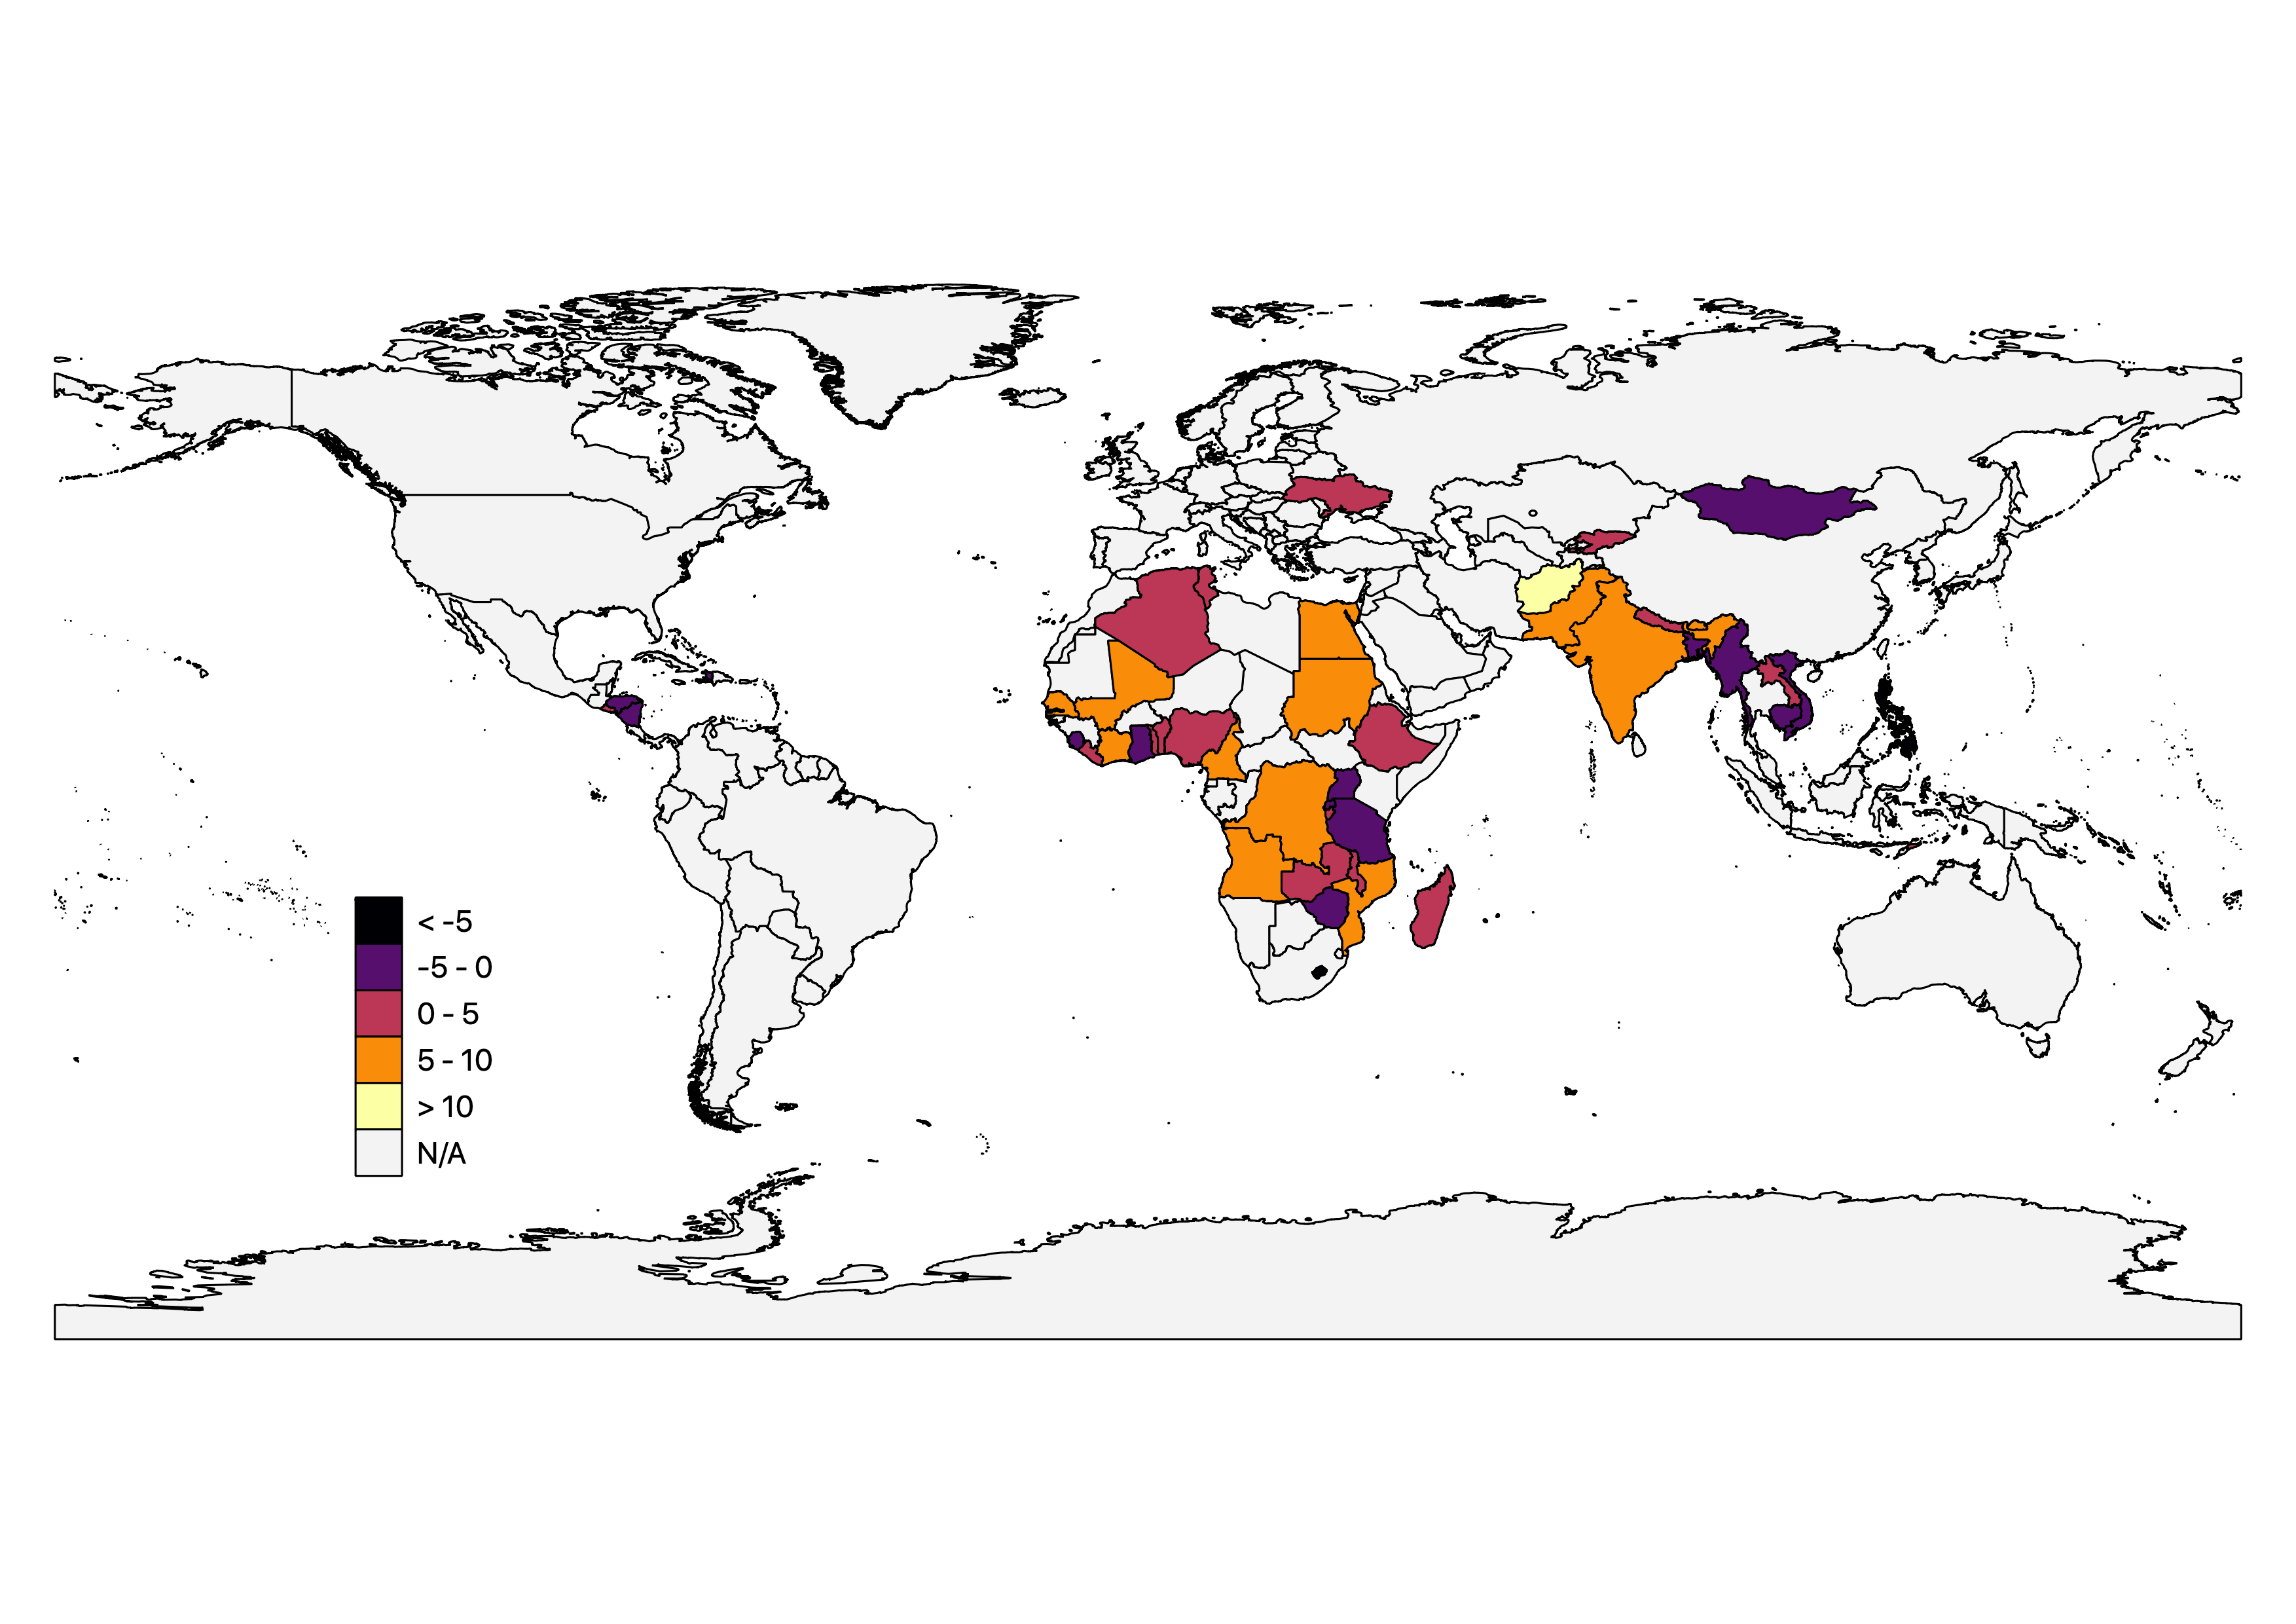
\includegraphics[width=1\linewidth,]{figures/maps/diff_YLILI} 

}

\caption{Gender differences in YLILI score}\label{fig:fig-gendiff}
\end{figure}

\begin{figure}[H]

{\centering 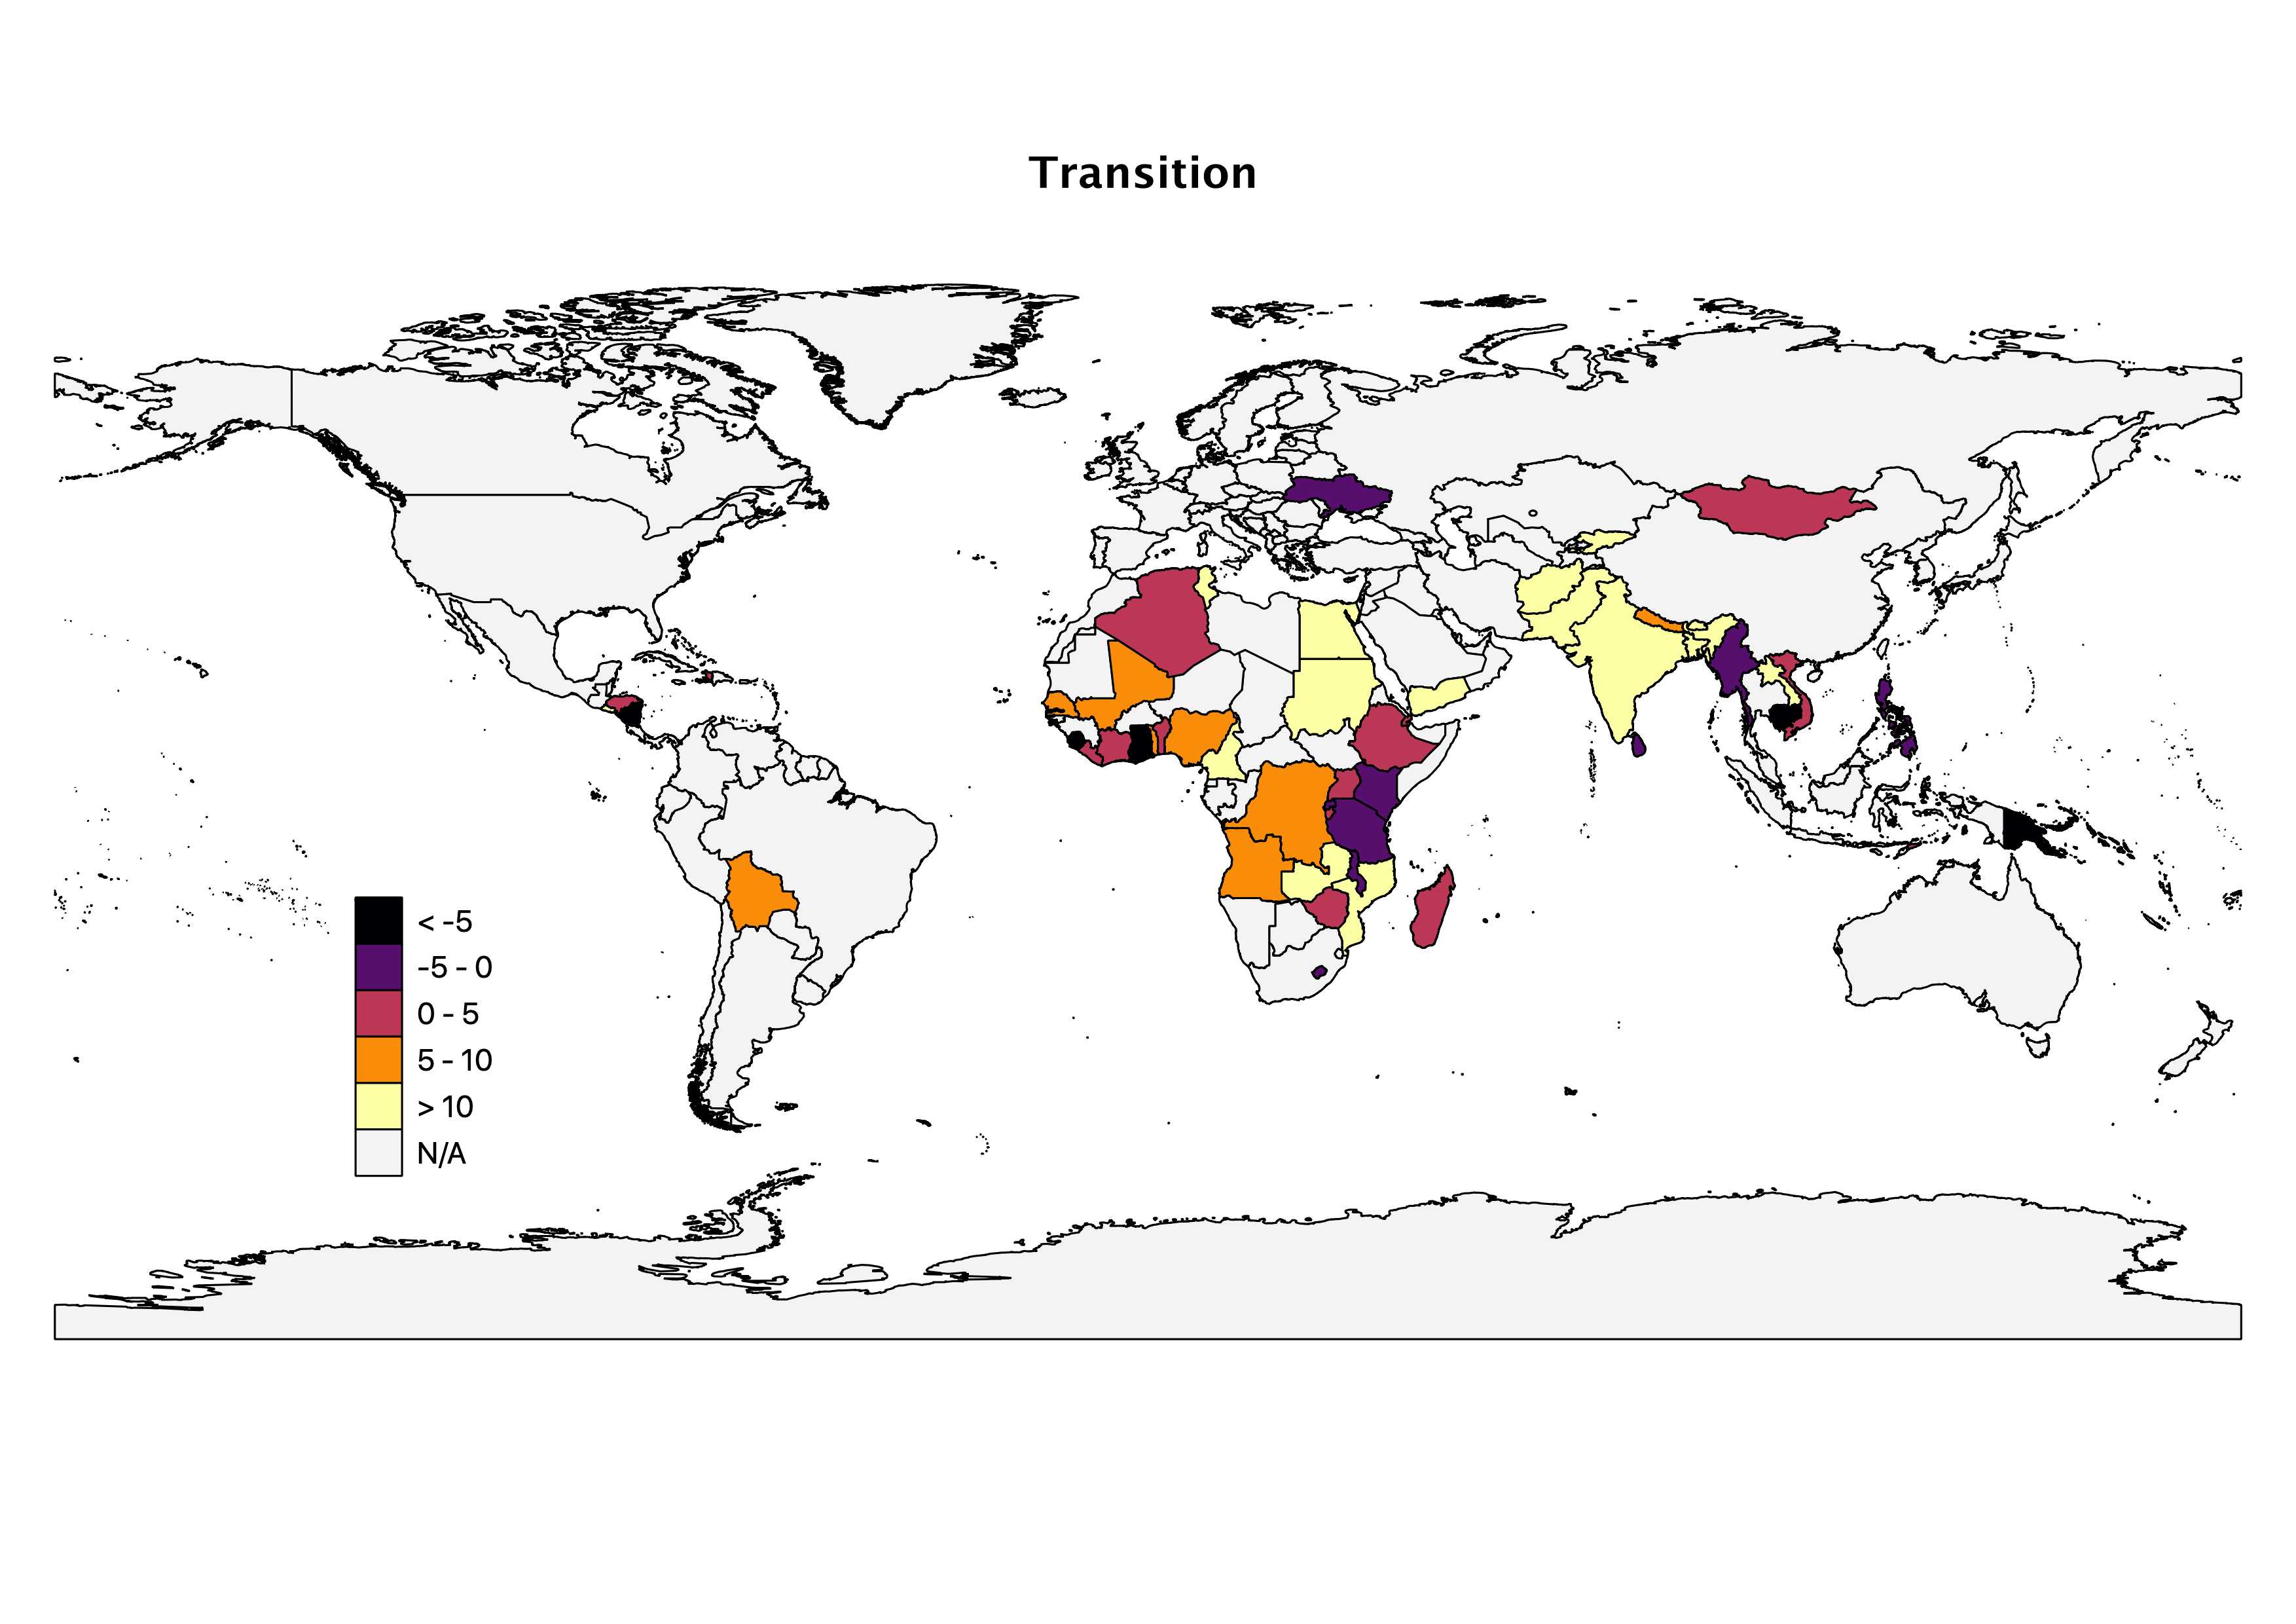
\includegraphics[width=0.69\linewidth,]{figures/maps/diff_transition} 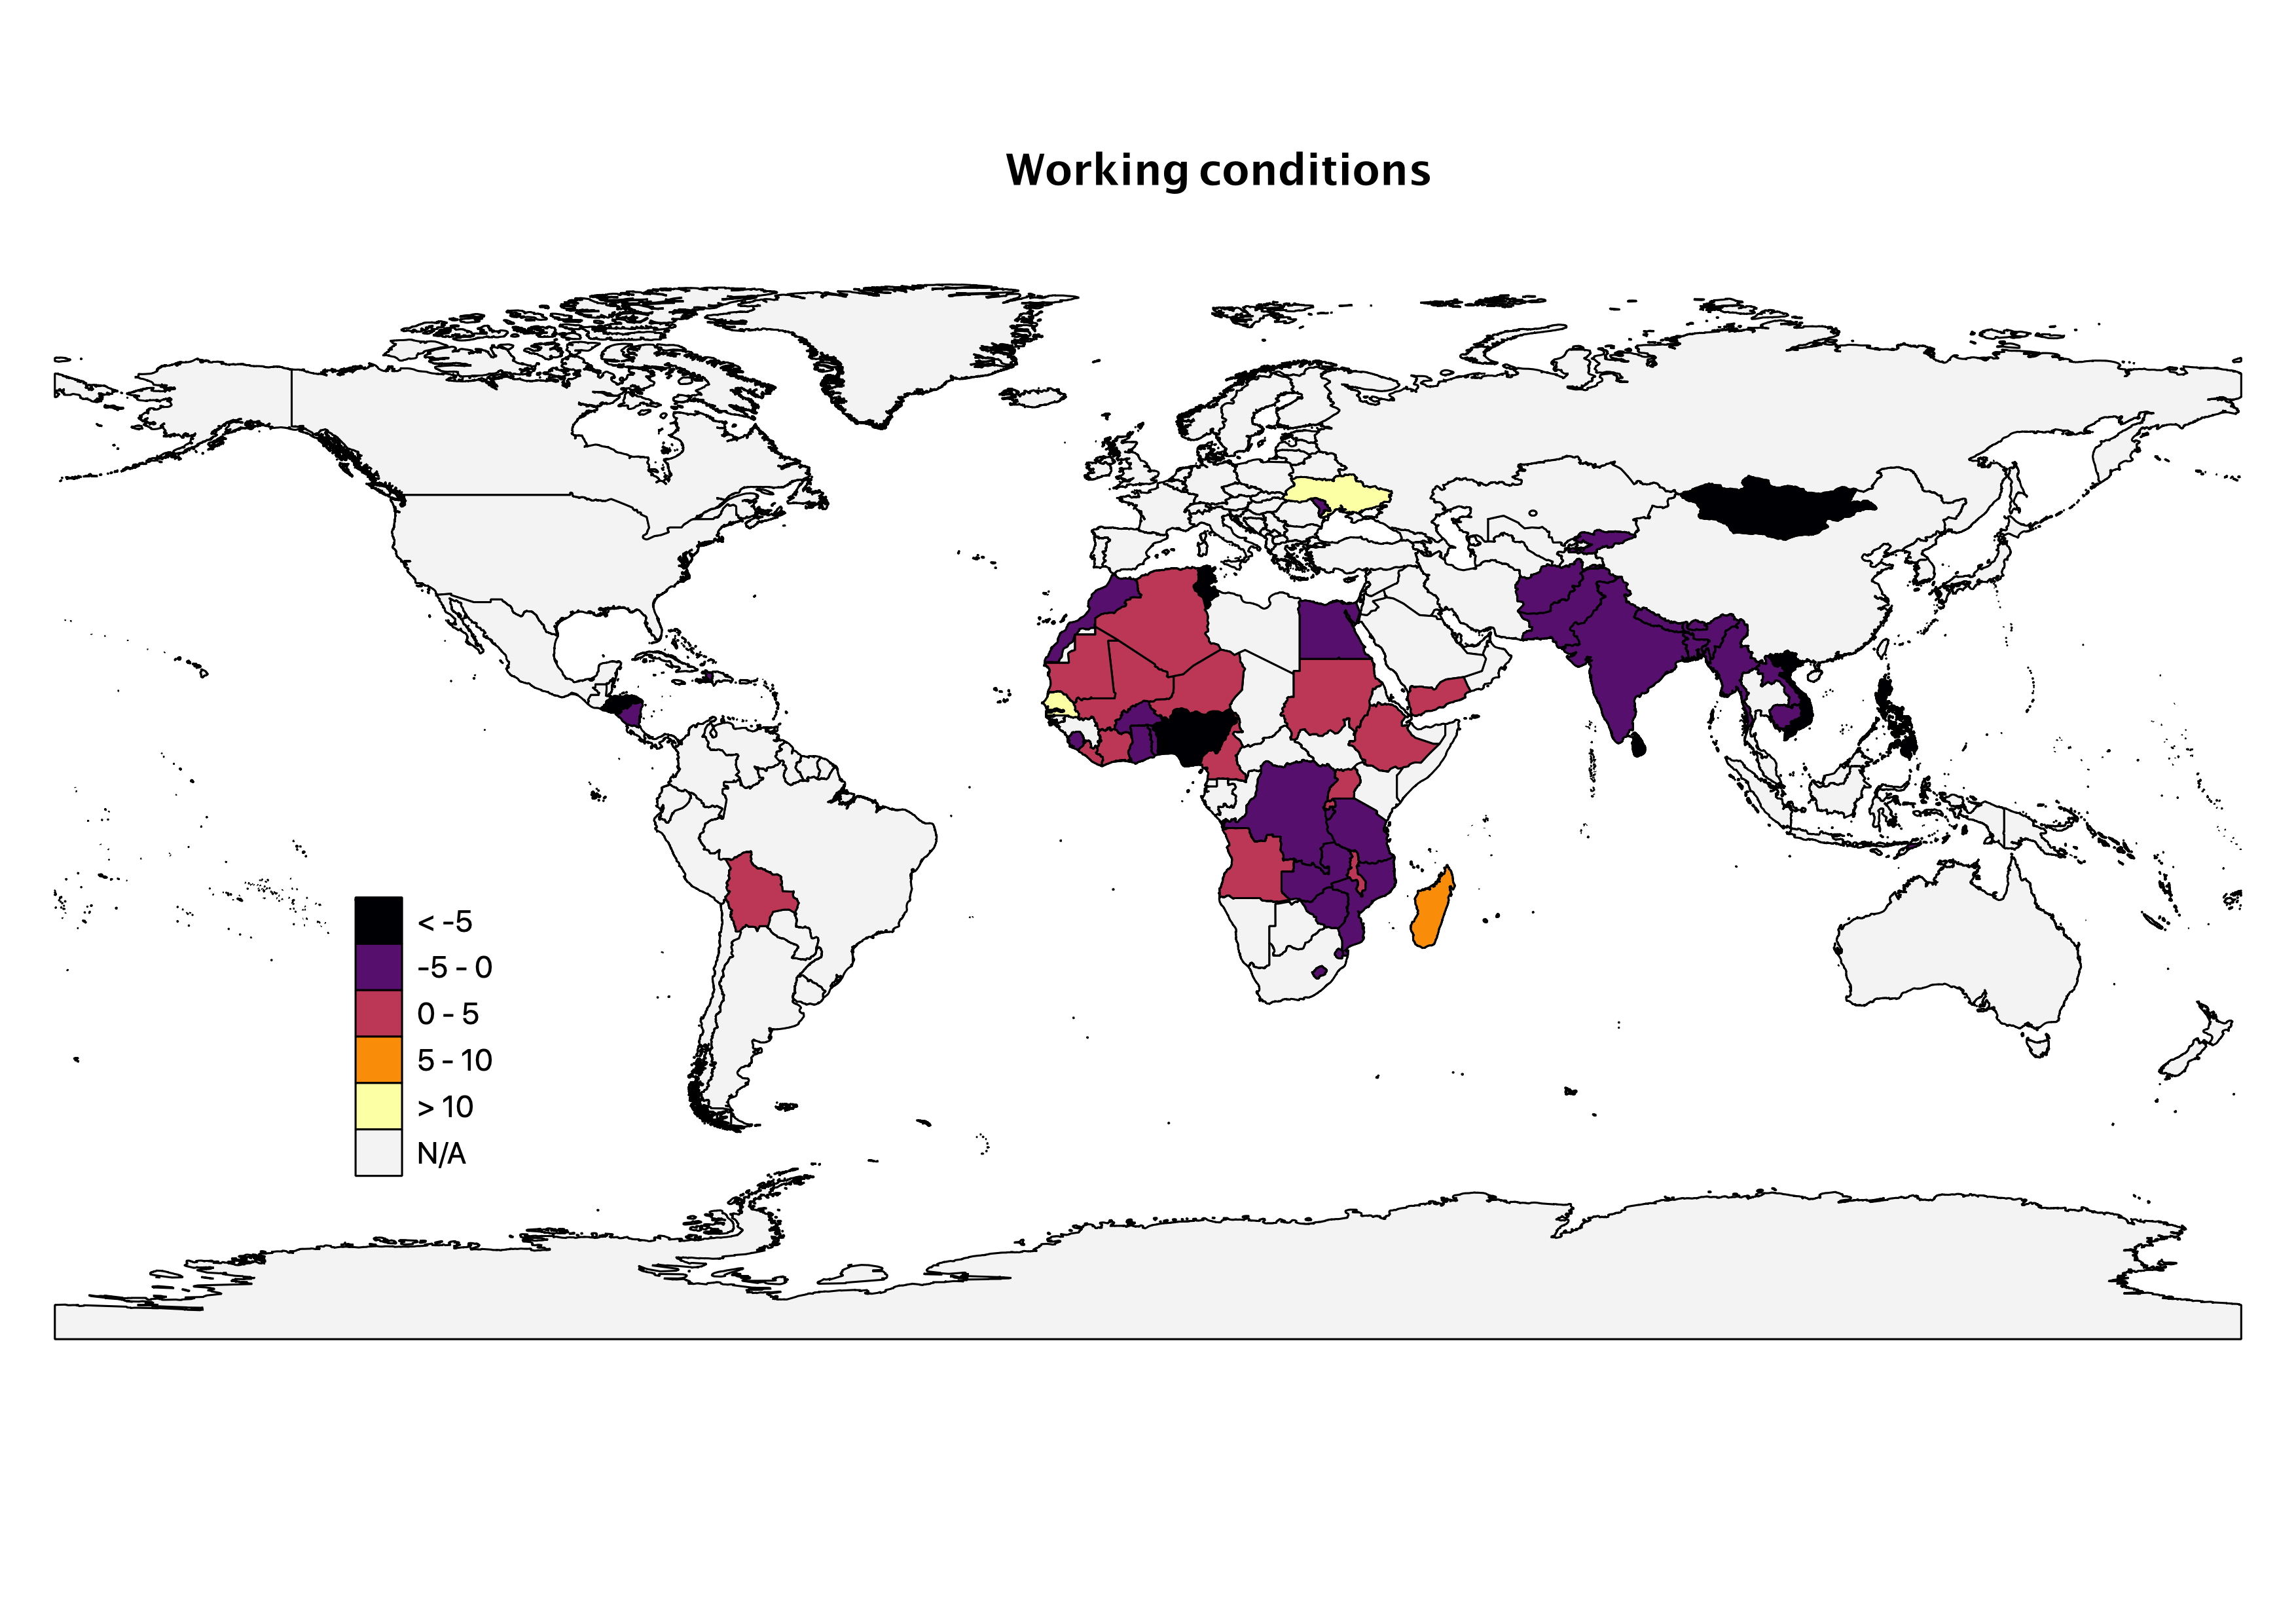
\includegraphics[width=0.69\linewidth,]{figures/maps/diff_working_conditions} 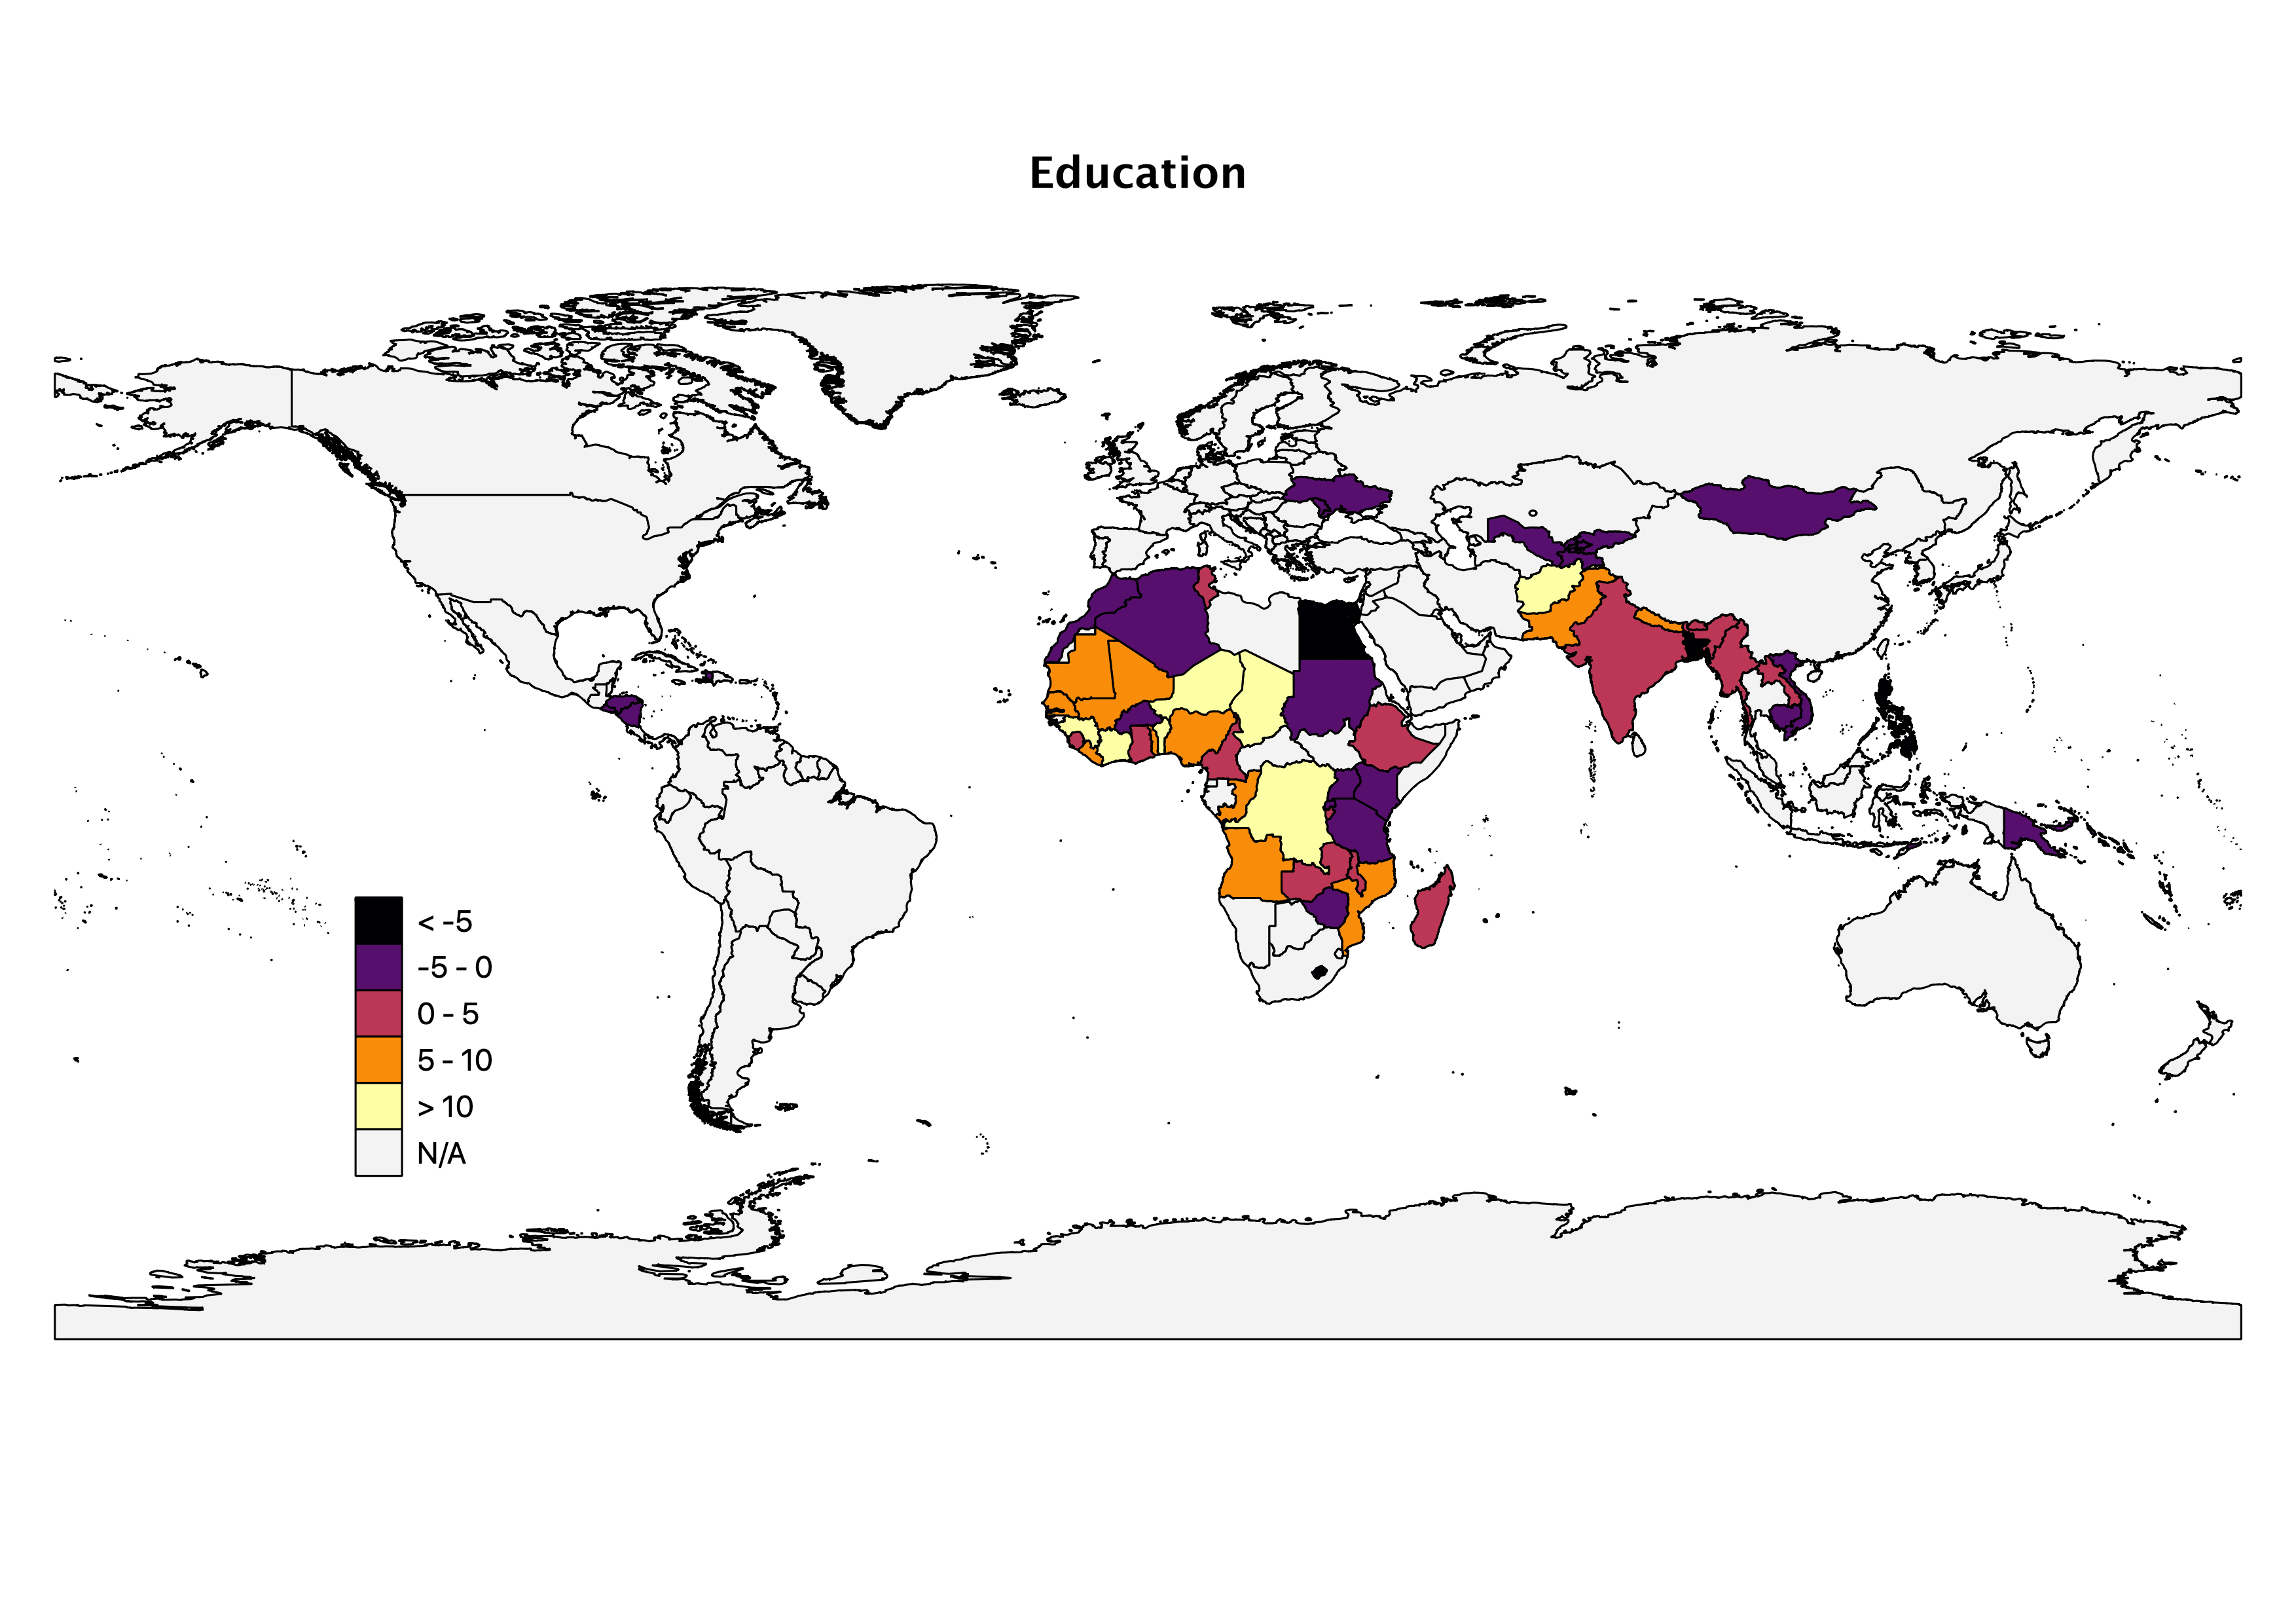
\includegraphics[width=0.69\linewidth,]{figures/maps/diff_education} 

}

\caption{Dimensions of the YLILI depicted by country}\label{fig:fig-genderdiffmaps}
\end{figure}

\newpage

\hypertarget{altscores}{%
\subsection*{Robustness}\label{altscores}}

\markboth{Robustness}{Appendix B2}

\begin{figure}[H]

{\centering 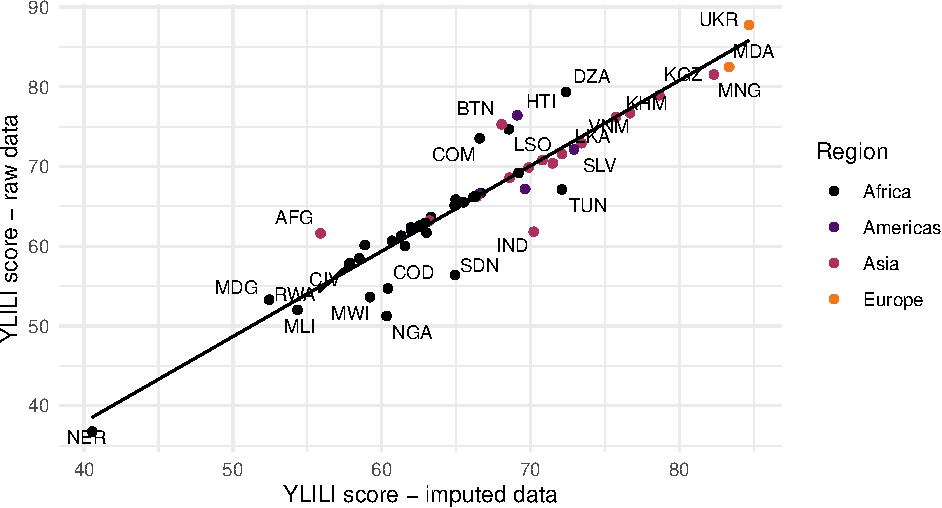
\includegraphics{figures/fig-arithgeom-1} 

}

\caption{Comparison of aggregation methods}\label{fig:fig-arithgeom}
\end{figure}

\begin{figure}[H]

{\centering 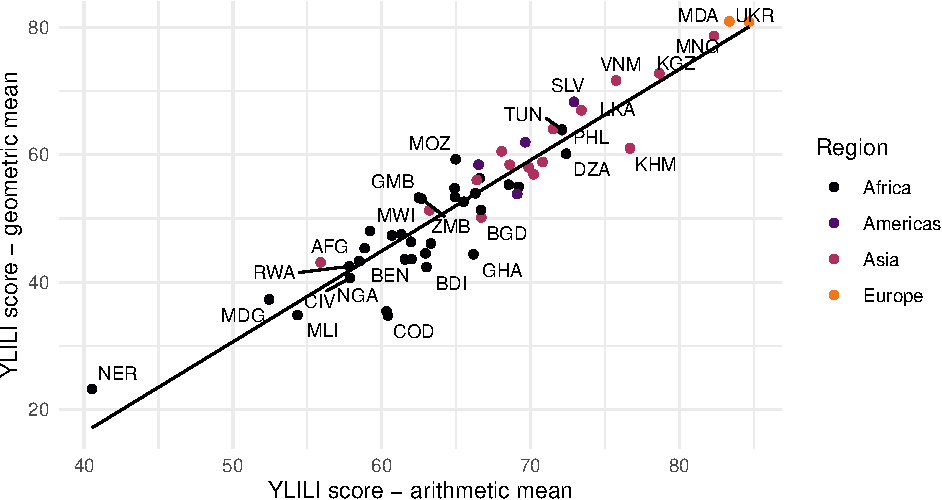
\includegraphics{figures/fig-imputedraw-1} 

}

\caption{YLILI with and without imputation}\label{fig:fig-imputedraw}
\end{figure}

\begin{landscape}

\begingroup
\floatsetup{capposition=top, font={scriptsize, tablefont}}
\setlength\LTleft{-3cm}
\begin{longtable}{lccccccccccccc} 
\caption{\textrm{\normalfont \small Alternative specifications (new ranking) \label{tab:tbl-altscores}}}
\\[-1.8ex]\hline 
\hline \\[-1.8ex] 
\rot{country} & \rot{YLILI} & \rot{no neet} & \rot{no relative wc} & \rot{no mismatch} & \rot{no workingpov} & \rot{no underemp} & \rot{no informal} & \rot{no elementary} & \rot{no nosecondary} & \rot{no literacy} & \rot{no test scores} & \rot{geometric} & \rot{raw} \\
\hline \\[-1.8ex] 
Ukraine & 84.67 (1) & 86.06 (2) & 83.74 (1) & 84.22 (1) & 83.77 (1) & 83.79 (1) & 89.5 (1) & 84.55 (1) & 83.2 (1) & 81.65 (1) & 89.17 (1) & 80.87 (2) & 87.74 (1) \\ 
Moldova & 83.36 (2) & 86.13 (1) & 81.42 (2) & 82.52 (2) & 81.97 (2) & 82.16 (2) & 84.24 (4) & 83.57 (2) & 82.48 (2) & 79.03 (2) & 88.56 (2) & 80.93 (1) & 82.48 (2) \\ 
Mongolia & 82.32 (3) & 84.25 (3) & 81.03 (3) & 81.69 (3) & 81.34 (3) & 81.41 (3) & 86.16 (2) & 82.16 (3) & 81.55 (3) & 77.94 (3) & 87.48 (3) & 78.65 (3) & 81.55 (3) \\ 
Kyrgyzstan & 78.66 (4) & 79.7 (4) & 77.32 (5) & 78.94 (4) & 77.62 (4) & 77.95 (4) & 83.84 (5) & 80.56 (4) & 75.18 (6) & 75.16 (4) & 85.63 (4) & 72.78 (4) & 78.94 (5) \\ 
Cambodia & 76.69 (5) & 76.73 (5) & 76.24 (6) & 77.1 (5) & 77.39 (5) & 76.46 (5) & 84.52 (3) & 77.78 (5) & 77.35 (4) & 72.57 (6) & 80.15 (5) & 61 (12) & 76.69 (6) \\ 
Viet Nam & 75.75 (6) & 73.89 (7) & 79.49 (4) & 73.88 (6) & 72.89 (6) & 72.63 (7) & 78.8 (7) & 75.25 (6) & 76.23 (5) & 72.93 (5) & 78.1 (10) & 71.64 (5) & 76.23 (8) \\ 
Sri Lanka & 73.43 (7) & 74.2 (6) & 72.79 (7) & 73.28 (7) & 71.77 (7) & 71.97 (8) & 78.3 (8) & 73.68 (8) & 72.93 (7) & 68.01 (8) & 79.34 (6) & 66.98 (7) & 72.93 (12) \\ 
El Salvador & 72.92 (8) & 73.57 (10) & 72.63 (8) & 72.57 (8) & 70.8 (12) & 71.28 (10) & 77.09 (12) & 73.59 (9) & 72.15 (8) & 68.63 (7) & 77.99 (12) & 68.32 (6) & 72.15 (13) \\ 
Algeria & 72.39 (9) & 73.86 (8) & 70.82 (11) & 72.5 (9) & 71.44 (9) & 73.14 (6) & 79.13 (6) & 72.76 (11) & 71.92 (9) & 66.41 (11) & 78.85 (8) & 60.17 (14) & 79.34 (4) \\ 
Philippines & 72.12 (10) & 73.07 (12) & 70.8 (12) & 72.5 (10) & 71.45 (8) & 71.89 (9) & 77.45 (10) & 74.49 (7) & 71.58 (11) & 65.71 (15) & 79.07 (7) & 63.85 (10) & 71.58 (14) \\ 
Tunisia & 72.11 (11) & 73.61 (9) & 70.5 (14) & 72.22 (12) & 70.82 (11) & 71.1 (11) & 77.74 (9) & 73.54 (10) & 71.67 (10) & 66.47 (10) & 78.19 (9) & 63.97 (9) & 67.12 (21) \\ 
Palestine & 71.5 (12) & 73.01 (13) & 71.56 (10) & 69.94 (16) & 68.63 (21) & 68.81 (17) & 75.76 (17) & 71.32 (13) & 70.41 (12) & 66.66 (9) & 77.45 (13) & 64.02 (8) & 70.41 (16) \\ 
Nepal & 70.81 (13) & 73.44 (11) & 69.4 (16) & 69.58 (19) & 68.93 (20) & 69.35 (15) & 76.25 (15) & 70.62 (14) & 68.19 (15) & 66.18 (14) & 78.06 (11) & 58.86 (16) & 70.81 (15) \\ 
India & 70.22 (14) & 70.92 (14) & 68.62 (17) & 71.11 (13) & 69.42 (17) & 69.19 (16) & 76.57 (13) & 70 (16) & 67.64 (18) & 66.41 (12) & 76.61 (14) & 56.93 (20) & 61.82 (38) \\ 
Timor-Leste & 69.88 (15) & 69.73 (16) & 70.21 (15) & 69.71 (18) & 69.64 (16) & 68.04 (19) & 75.73 (18) & 68.42 (21) & 67.03 (23) & 66.18 (13) & 76.44 (15) & 58.03 (19) & 69.88 (17) \\ 
Nicaragua & 69.65 (16) & 67.35 (25) & 71.86 (9) & 69.73 (17) & 69.65 (15) & 70.87 (12) & 75.56 (19) & 69.98 (18) & 69.23 (13) & 64.58 (18) & 75.13 (18) & 61.96 (11) & 67.18 (20) \\ 
Cameroon & 69.2 (17) & 68.99 (19) & 66.24 (22) & 72.38 (11) & 70.92 (10) & 70.12 (13) & 77.29 (11) & 69.98 (17) & 67.54 (20) & 64.96 (17) & 75.1 (19) & 54.96 (24) & 69.2 (18) \\ 
Haiti & 69.11 (18) & 70.07 (15) & 67.04 (21) & 70.23 (14) & 69.77 (14) & 69.61 (14) & 76.45 (14) & 70.25 (15) & 66.75 (24) & 64.35 (19) & 76.24 (16) & 53.83 (27) & 76.44 (7) \\ 
Myanmar & 68.6 (19) & 66.68 (30) & 70.5 (13) & 68.61 (21) & 66.52 (25) & 66.76 (20) & 74.23 (20) & 68.47 (20) & 68 (16) & 65.03 (16) & 72.77 (22) & 58.42 (18) & 68.6 (19) \\ 
Lesotho & 68.54 (20) & 68.83 (20) & 67.77 (18) & 69.03 (20) & 69.87 (13) & 68.4 (18) & 75.98 (16) & 72.75 (12) & 67.85 (17) & 64.06 (20) & 73.73 (21) & 55.31 (23) & 74.68 (10) \\ 
Bhutan & 68.07 (21) & 68.46 (22) & 65.66 (23) & 70.08 (15) & 66.44 (27) & 66.54 (21) & 73.24 (21) & 67.08 (23) & 67.56 (19) & 62.79 (22) & 73.85 (20) & 60.54 (13) & 75.3 (9) \\ 
Bangladesh & 66.69 (22) & 67.15 (26) & 65.5 (24) & 67.42 (23) & 65.53 (30) & 65.34 (25) & 73.16 (22) & 66.29 (25) & 67.47 (21) & 60.15 (31) & 72.46 (23) & 50.16 (34) & 66.69 (22) \\ 
Uganda & 66.67 (23) & 69.44 (18) & 65.28 (26) & 65.29 (28) & 67.86 (23) & 65.47 (23) & 73.01 (23) & 66.51 (24) & 68.84 (14) & 60.63 (27) & 70.55 (30) & 51.33 (32) & 66.67 (23) \\ 
Comoros & 66.58 (24) & 67.47 (24) & 67.68 (20) & 64.6 (30) & 65.42 (31) & 64.53 (29) & 71.55 (27) & 65.35 (28) & 65.11 (29) & 63.16 (21) & 71.48 (28) & 56.32 (21) & 73.53 (11) \\ 
Honduras & 66.51 (25) & 67.54 (23) & 64.37 (29) & 67.62 (22) & 66.45 (26) & 66.26 (22) & 72.64 (25) & 68.92 (19) & 67.22 (22) & 60.67 (26) & 71.64 (26) & 58.44 (17) & 66.51 (24) \\ 
Laos & 66.39 (26) & 68.5 (21) & 67.7 (19) & 62.96 (36) & 63.11 (38) & 62.42 (35) & 69.73 (34) & 63.17 (38) & 66.23 (25) & 60.51 (29) & 72.42 (24) & 56.02 (22) & 66.23 (26) \\ 
Togo & 66.3 (27) & 67.05 (27) & 65.14 (27) & 66.71 (25) & 68.37 (22) & 65.04 (27) & 72.76 (24) & 65.93 (26) & 65.22 (27) & 61.96 (23) & 71.72 (25) & 53.95 (26) & 66.3 (25) \\ 
Ghana & 66.17 (28) & 66.84 (28) & 65.4 (25) & 66.26 (26) & 64.93 (33) & 65.41 (24) & 71.73 (26) & 64.75 (30) & 62.88 (37) & 60.29 (30) & 75.33 (17) & 44.38 (42) & 66.17 (27) \\ 
Zimbabwe & 65.51 (29) & 69.7 (17) & 62.53 (34) & 64.3 (31) & 66.1 (28) & 64.94 (28) & 71.3 (28) & 67.21 (22) & 63.65 (33) & 61.37 (24) & 71.51 (27) & 52.61 (31) & 65.51 (29) \\ 
Mozambique & 64.97 (30) & 65.86 (34) & 61.72 (35) & 67.35 (24) & 69.31 (18) & 65.22 (26) & 67.31 (42) & 65.02 (29) & 65.56 (26) & 60.52 (28) & 68.84 (34) & 59.29 (15) & 65.86 (28) \\ 
Sudan & 64.94 (31) & 66.31 (31) & 63.38 (31) & 65.12 (29) & 63.48 (37) & 63.36 (30) & 70.86 (29) & 64.27 (31) & 64.69 (31) & 61.02 (25) & 69.1 (32) & 53.38 (28) & 56.42 (48) \\ 
Egypt & 64.9 (32) & 64.12 (37) & 64.73 (28) & 65.85 (27) & 62.89 (39) & 62.69 (34) & 69.98 (32) & 63.33 (37) & 65.09 (30) & 58.89 (36) & 70.72 (29) & 54.75 (25) & 65.09 (30) \\ 
Sierra Leone & 63.31 (33) & 62.74 (39) & 63.5 (30) & 63.69 (32) & 66.83 (24) & 63.36 (31) & 70.08 (31) & 63.6 (34) & 59.72 (43) & 59.96 (33) & 70.25 (31) & 46.07 (39) & 63.69 (31) \\ 
Pakistan & 63.2 (34) & 64.14 (36) & 62.58 (33) & 62.9 (37) & 61.06 (46) & 61.02 (40) & 68.35 (37) & 62.56 (39) & 63.39 (35) & 57.89 (38) & 68.33 (36) & 51.27 (33) & 63.2 (32) \\ 
Burundi & 63.01 (35) & 62.32 (42) & 63.14 (32) & 63.58 (34) & 69 (19) & 63.26 (32) & 70.72 (30) & 65.78 (27) & 65.19 (28) & 57.72 (39) & 66.13 (40) & 42.37 (48) & 61.7 (39) \\ 
Senegal & 62.94 (36) & 65.05 (35) & 60.12 (38) & 63.66 (33) & 64.74 (36) & 62.31 (36) & 69.88 (33) & 63.58 (35) & 63.05 (36) & 59.98 (32) & 65.79 (41) & 44.51 (41) & 62.94 (33) \\ 
Zambia & 62.67 (37) & 66.06 (32) & 61.04 (36) & 60.9 (44) & 64.77 (35) & 60.56 (41) & 67.17 (43) & 62.17 (41) & 62.32 (39) & 56.66 (41) & 69.02 (33) & 53.12 (30) & 62.67 (34) \\ 
Gambia & 62.5 (38) & 66.77 (29) & 59.45 (42) & 61.28 (42) & 60.72 (47) & 60.5 (42) & 67.06 (44) & 63.36 (36) & 60.53 (42) & 59.24 (35) & 67.72 (38) & 53.26 (29) & 62.5 (35) \\ 
Burkina Faso & 62 (39) & 66.01 (33) & 59.96 (39) & 60.03 (47) & 62.48 (41) & 59.68 (46) & 67.84 (39) & 60.2 (46) & 64.25 (32) & 58.67 (37) & 63.07 (46) & 43.61 (43) & 62 (37) \\ 
Liberia & 61.97 (40) & 62.51 (41) & 61.04 (37) & 62.35 (39) & 65.74 (29) & 63.25 (33) & 69.29 (35) & 62.19 (40) & 59.12 (45) & 59.59 (34) & 67.19 (39) & 46.34 (38) & 62.35 (36) \\ 
Mauritania & 61.56 (41) & 63.71 (38) & 59.73 (40) & 61.26 (43) & 59.98 (49) & 59.81 (45) & 67.71 (41) & 60.9 (44) & 61.63 (40) & 57.28 (40) & 65.78 (42) & 43.58 (44) & 60.03 (44) \\ 
Tanzania & 61.32 (42) & 61.09 (44) & 59.7 (41) & 63.15 (35) & 64.91 (34) & 62.1 (38) & 68.99 (36) & 64.03 (32) & 63.56 (34) & 55.32 (44) & 65.07 (44) & 47.52 (36) & 61.32 (41) \\ 
Ethiopia & 60.69 (43) & 60.68 (45) & 59.42 (43) & 61.98 (40) & 62.37 (42) & 62.28 (37) & 68.22 (38) & 64.02 (33) & 62.67 (38) & 54.88 (46) & 64.53 (45) & 47.33 (37) & 60.69 (42) \\ 
DR Congo & 60.41 (44) & 60.09 (47) & 58.7 (45) & 62.44 (38) & 65.29 (32) & 60.47 (43) & 67.75 (40) & 60.35 (45) & 57.69 (48) & 54.96 (45) & 68.6 (35) & 34.77 (53) & 54.71 (49) \\ 
Nigeria & 60.33 (45) & 62.53 (40) & 58.82 (44) & 59.63 (48) & 62.08 (43) & 59.85 (44) & 66.72 (45) & 61.39 (43) & 57.39 (49) & 55.77 (43) & 67.81 (37) & 35.42 (51) & 51.25 (53) \\ 
Malawi & 59.22 (46) & 61.66 (43) & 57.69 (46) & 58.3 (49) & 62.71 (40) & 57.97 (48) & 64.86 (49) & 58.58 (49) & 60.61 (41) & 53.97 (48) & 63.07 (47) & 48.01 (35) & 53.61 (50) \\ 
Angola & 58.86 (47) & 58.12 (51) & 56.75 (47) & 61.7 (41) & 62.01 (44) & 58.13 (47) & 65.28 (47) & 57.98 (50) & 57.09 (51) & 53.96 (49) & 65.53 (43) & 45.34 (40) & 60.16 (43) \\ 
Benin & 58.49 (48) & 58.3 (50) & 56.36 (48) & 60.81 (45) & 61.82 (45) & 61.48 (39) & 66.36 (46) & 59.93 (47) & 57.9 (47) & 55.86 (42) & 61.71 (49) & 43.3 (45) & 58.49 (45) \\ 
Côte d'Ivoire & 57.87 (49) & 58.71 (49) & 54.42 (50) & 60.49 (46) & 58.75 (51) & 57.37 (50) & 64.96 (48) & 57.98 (51) & 57.95 (46) & 54.85 (47) & 60.83 (50) & 40.65 (49) & 57.87 (46) \\ 
Rwanda & 57.82 (50) & 60.59 (46) & 55.44 (49) & 57.43 (50) & 60.32 (48) & 57.66 (49) & 64.41 (50) & 62.07 (42) & 59.32 (44) & 51.36 (50) & 62.79 (48) & 42.49 (47) & 57.82 (47) \\ 
Afghanistan & 55.89 (51) & 58.8 (48) & 53.98 (51) & 54.9 (53) & 56.76 (53) & 55.39 (52) & 61.38 (51) & 54.8 (52) & 57.26 (50) & 51.16 (51) & 59.25 (51) & 43.1 (46) & 61.62 (40) \\ 
Mali & 54.34 (52) & 53.64 (52) & 52.03 (52) & 57.34 (51) & 57.14 (52) & 53.27 (53) & 61.27 (52) & 53.65 (53) & 52.85 (53) & 51.09 (52) & 59.07 (52) & 34.83 (52) & 52.03 (52) \\ 
Madagascar & 52.43 (53) & 51.13 (53) & 50.86 (53) & 55.31 (52) & 59.01 (50) & 56.48 (51) & 60.79 (53) & 58.98 (48) & 53.3 (52) & 46.53 (53) & 57.46 (53) & 37.3 (50) & 53.3 (51) \\ 
Niger & 40.54 (54) & 41.93 (54) & 40.26 (54) & 39.44 (54) & 38.53 (54) & 35.75 (54) & 43.19 (54) & 36.05 (54) & 40.43 (54) & 37.1 (54) & 44.09 (54) & 23.25 (54) & 36.75 (54) \\ 
\hline \\[-1.8ex]
\end{longtable}
\endgroup

\end{landscape}

\renewcommand{\thesection}{\arabic{chapter}.\arabic{section}}
\setcounter{section}{0}
\renewcommand{\thesubsection}{\arabic{chapter}.\arabic{section}.\arabic{subsection}}
\setcounter{subsection}{0}

\newsection

\chapter[Lost in Transition]{Lost in Transition: School-to-Work Transition Mapping in Urban Bénin}

\begin{chapabstract}
This paper uses a novel, longitudinal dataset of 752 youth aged 20-29 in Cotonou, Benin, to map school-to-work transitions (SWTs) in a highly informal, urban economy. Five waves of in-person and mobile phone surveys conducted over three years provide rich employment and activity histories for youth. First, the activity histories are used to estimate the duration of the transition from school to employment. Second, transition matrices constructed from the event histories are used identify differences in rates of transition between activity states by gender and age group. Third, Optimal Matching Analysis (OMA) treats the activity histories as sequences, allowing us to group and analyze clusters of similar school-to-work trajectories. Fourth, we develop a detailed taxonomy of employment types (such as casual work or independent self-employment) and analyze the propensity for youth to engage in or transition into these types of work. We document limited permeation between activity states, a low probability of exiting the SWT among young women, and a late school-leaving age among all youth. We interpret the latter as indicative of strong sorting in the early stages of the SWT in informal labor markets.

\end{chapabstract}

\newpage

\onehalfspacing

\hypertarget{survey-intro}{%
\section{\texorpdfstring{Introduction \hl{and Background}}{Introduction }}\label{survey-intro}}

\todo{7}

The youth population in Sub-Saharan Africa (SSA) is growing rapidly, and is expected to continue to do so for the foreseeable future. This presents both challenges and opportunities for the region. Despite recent increases in educational levels in sub-Saharan Africa, which have increased young people's potential to become gainfully employed, youth continue to face many challenges when leaving school and seeking work. Youth in low-income countries (LICs) are more likely to be unemployed or to work informally than adults \autocite{quintini2014}, yet they constitute a significant proportion of the population in the region, and their ability to find employment and enter the labour market has significant implications for economic growth and development.

\todo{7}\hl{Studying the school-to-work transition (SWT) and the linkages between education and employment is crucial to assessing the performance of young people in the labor market.} The transition to the labour market marks a critical point in the productive and social development of young individuals. Delayed entry into formal employment has been shown to depress future earnings in high-income and developing countries alike \autocite{bridges2017}, while a semi-permanent state of ``waithood'' is commonly reported among youth (particularly males) in SSA, impeding their social integration and undermining the self-worth of those unable to find employment \autocite{mains2011,honwana2012}. \hlc[lightgray]{Those youth who find work tend to be underemployed and in informal jobs, leading to youth poverty, exacerbating inequality, and fostering unrest and conflict, raising the possibility of youth unrest observed elsewhere in the world }\autocite{urdal2006,mains2011}.

\todo{7}\hl{Researchers are particularly interested in three key aspects of the SWT: the duration of the job search after completing education, the fluidity of the transition (marked by the presence or absence of inactivity or unemployment spells), and the potential correlation between a smooth school-to-work transition and future labor market success.} \hlc[lightgray]{Both the age of school-leaving and the speed of transition to the labour market are of particular interest to policy makers in SSA, where young people (aged 15-24) suffer over twice the unemployment rate of adults, albeit with high variation across countries }\autocite{africandevelopmentbank2016a}. \hlc[lightgray]{A delayed entry into the labour force can reduce youths' lifetime labour market participation and contribution to the economy, while slow transition can result in employment "scarring": early periods of underemployment and unemployment that lead to wage losses and reduce the likelihood of returning to the labour force. Evidence from high-income countries suggests that protracted unemployment spells, including extended school-to-work transitions, negatively affect future earnings and employment prospects} \autocite{schmillen2017,emmenegger2017,moller2015,cockx2012}. \hl{Understanding the factors that influence the transition into the labour market can help policymakers and other stakeholders identify and implement interventions that can improve youth's employment prospects and economic outcomes in adulthood. Studying the SWT can also provide insight into the broader socioeconomic dynamics of the region and can help to inform policy decisions in other areas, such as education and training.}

\todo{8}\hl{Unfortunately, the lack of standardized data and comparable indicators presents a significant obstacle to analyzing this crucial period, especially in lower-middle income countries (LMICs) and LICs, where access to panel data is limited. While standard labor market indicators such as youth employment and unemployment rates are often used to describe the SWT, they provide a static snapshot of a dynamic process. Research on youth labor dynamics reveals a more nuanced reality: only a minority transition directly to stable employment or sustained inactivity. Many navigate a dynamic path marked by multiple job changes, unemployment spells, and labor market exits and re-entries before finding stability or opting for alternative pursuits like extended breaks or further education. This highlights the need for frameworks and indicators that encompass this complexity and capture the diverse and fluid trajectories of young people entering the workforce.}

\hl{This study delves into these complex dynamics in Cotonou, Bénin, a city characterized by a predominantly informal economic landscape. Utilizing a novel, longitudinal dataset from a survey conducted with 752 youth, we track youth movements between school, employment, and inactivity to map the SWT in an urban, highly informal economy. We analyze both panel observations and employment histories to calculate the age of school-leaving, the age of labor market entry, the duration of the transition, and the propensity to switch between different employment states. We also deploy a novel methodology called Optimal Matching Analysis to identify and quantify the most prevalent pathways young people follow after leaving full-time education in Cotonou.}

The paper is organized as follows. We review the extant literature on SWT, focusing on evidence from LICs, in Section \ref{survey-litreview}. Section \ref{survey-datamethods} presents the data and methodology used in the paper. Section \ref{survey-results} contains analysis and results, and Section \ref{survey-conclusion} concludes.

\hypertarget{survey-litreview}{%
\section{\texorpdfstring{\hl{Literature Review}}{}}\label{survey-litreview}}

\todo{7,9}\hlc[pink]{The dynamic process of the school-to-work transition (SWT), including all the activities of young people between full-time schooling and stable employment, can only be fully captured with detailed, longitudinal data; as a result, most studies of SWT dynamics to date have been conducted in high-income countries (HICs).} In addition to data scarcity, the informality inherent to most youth labour markets in the low- and middle-income countries render traditional data sources insufficient for capturing all the details of the SWT. While the path from formal education to formal employment is sequential and quantifiable, the SWT in informal labour markets tends to be more complicated, often leading through halting periods of formal education and informal training, stints working for the family firm, prolonged school absences or repeated years, and extended periods of economic inactivity. Official labour market data in developing countries is too infrequent and unreliable to capture such dynamics.

\todo{8}\hl{Cross-sectional data, commonly used to describe labor market transitions, suffers from several flaws: it assumes universal education and employment, overlooks individual variations, reflects different cohorts at a single point, and fails to capture informal work} \autocite{nilsson2019}. \hl{Event history and panel data offer some advantages, as transition statistics can be computed at an individual level, though bias can arise if only completed transitions are considered. To counter this drawback, researchers often rely on survival analysis to study the determinants of transition age or duration, even in the presence of right-censored transition data} \autocite{nordman2015,manacorda2017}. \hl{Panel data has also been used to construct transition matrices for employment states, which allow for the calculation of various statistics such as the degree of turnover, the probabilities of leaving a particular sector such as unemployment, or the duration of any given state, such as the transition from school to work, though are limited in their interpretability due to the large number of matrices that such an analyses generates} \autocite{cunningham2011,bridges2017}. \hl{In order to benefit from each of these methods' advantages while limiting our exposure to their drawbacks, we rely on a combination of these approaches in this paper.}

\hl{Two counteracting factors are generally understood to affect the SWT duration in SSA. Poverty and lack of unemployment insurance lowers reservation wages and drives youth into work sooner, reducing the duration of the SWT, while increasing education and decreasing number of public sector jobs drives up employment expectations without matching wage job growth, which tends to prolong the SWT as youth wait for an opportunity commensurate with their expecatation and education level.} \hlc[lightgray]{Lower reservation wages and accelerated transitions lead to worse employment matches, as measured by the probability of attaining stable employment in the long run }\autocite{manacorda2017}, \hl{while inflated employment expectations lead to longer periods of inactivity and employment scarring.}

\hl{Other factors also play a crucial role in determining the duration and smoothness of the SWT in LICs.} \hlc[lightgray]{Rising education rates in SSA mechanically delay the transition: as increasing numbers of youth stay in school for longer, they enter the labour market at a more advanced age }\autocite{calves2013}\hlc[lightgray]{. More educated youth in SSA, especially university graduates, have been shown to be reluctant to work in the informal sector, preferring to wait for formal or public sector employment }\autocite{serneels2007}\hlc[lightgray]{. Education mismatch may also prolong the SWT: if education systems are not aligned with the demands of the labour market, students may graduate with skills that are not in high demand, slowing the transition to wage work and increasing unemployment and underemployment for the most educated youth.} \textcite{bandara2019}\hlc[lightgray]{, using eight SWTS surveys from SSA (including Bénin), report that about 47 and 28 percent of employed youth in their sample are overqualified and under-qualified for their jobs, respectively. Finally, }\textcite{manacorda2017}\hlc[lightgray]{ report that women generally experience longer transition duration and are more likely to exit the labour market before completing the transition, taking twice as long as men to become employed after leaving school in certain LICs.}

\todo{9} \hl{Table }\ref{tab:tbl-desc} \hl{summarizes the comparative literature on the school-to-work transition.} \hlc[lightgray]{Though there is much heterogeneity in the data, youth from the highest-income and lowest-income countries are observed to have relatively short school-to-work transitions, though youth in HICs stay in school longer and have lower rates of inactivity after school-leaving }\autocite{manacorda2017,quintini2014}. The longest observed SWT duration is observed in middle-income countries in LAC, MENA, and southern Europe. Compared to HICs, out-of-school youth in LICs are more likely to become NEET upon leaving school, and under-employment is more widespread \autocite{quintini2014}. Moreover, competition for limited formal jobs is intensified in the presence of rapid population growth: \textcite{manacorda2017} find that a one standard deviation increase in the rate of population growth increases the time it takes youth to find work after leaving school by as much as 17 months\footnote{The authors also find that a one standard deviation increase the poverty rate leads to a reduction in transition duration of about 17 months and an increase in probability of never attaining employment of 14 percentage points.}.

\todo{9}

\begin{longtable}[]{@{}
  >{\raggedright\arraybackslash}p{(\columnwidth - 6\tabcolsep) * \real{0.2500}}
  >{\raggedright\arraybackslash}p{(\columnwidth - 6\tabcolsep) * \real{0.2500}}
  >{\raggedright\arraybackslash}p{(\columnwidth - 6\tabcolsep) * \real{0.2500}}
  >{\raggedright\arraybackslash}p{(\columnwidth - 6\tabcolsep) * \real{0.2500}}@{}}
\caption{\label{tab:litreview} \hl{Comparative Studies of School-to-work Transitions}}\tabularnewline
\toprule\noalign{}
\begin{minipage}[b]{\linewidth}\raggedright
\hl{Paper}
\end{minipage} & \begin{minipage}[b]{\linewidth}\raggedright
\hl{Data}
\end{minipage} & \begin{minipage}[b]{\linewidth}\raggedright
\hl{Method}
\end{minipage} & \begin{minipage}[b]{\linewidth}\raggedright
\hl{Results}
\end{minipage} \\
\midrule\noalign{}
\endfirsthead
\toprule\noalign{}
\begin{minipage}[b]{\linewidth}\raggedright
\hl{Paper}
\end{minipage} & \begin{minipage}[b]{\linewidth}\raggedright
\hl{Data}
\end{minipage} & \begin{minipage}[b]{\linewidth}\raggedright
\hl{Method}
\end{minipage} & \begin{minipage}[b]{\linewidth}\raggedright
\hl{Results}
\end{minipage} \\
\midrule\noalign{}
\endhead
\bottomrule\noalign{}
\endlastfoot
\textcite{manacorda2017} & \hl{ILO-STWT survey data from 23 LICs and LMICs} & \hl{Survival analysis for right-censored data} & \hl{Faster transitions in LICs vs LMIcs.} \\
\textcite{quintini2014} & \hl{OECD estimates based on labor force surveys} & \hl{Cross-sectional analysis (time needed for 50\% of youth to find work} & \hl{Low unemp. rates hide under- employment in LICS} \\
\textcite{cunningham2011} & \hl{Panel labor force surveys from Argentina, Brazil and Mexico} & \hl{Panel data analysis, including transition probabilities and duration in each state} & \hl{Common path is informal to formal sector, to self-employment later in life} \\
\textcite{quintini2009} & \hl{National Longitudinal Surveys in US and Europe} & \hl{Optimal Matching Analysis} & \hl{More turnover, shorter employment spells in US vs. Europe} \\
\end{longtable}

\todo{9} First labour market experience has also been emphasized as an important component of a successful SWT in the literature. \textcite{bridges2017} \hlc[pink]{use the Tanzania Household Urban Panel Survey to study how first experiences in the labour market effects future earnings, and find that school-leavers who immediately find a wage job experience a future wage premium, especially in the formal sector. Youth who attend private schooling in Ouagadougou, Burkina Faso were shown to be 9 percentage point more likely to find wage work as first employment }\autocite{calves2013}. \hlc[pink]{First work experience may even take place while youth are in school, though work-study statistics are often not captured in the data: using the School-to-Work Transition Surveys (SWTS),} \textcite{dedehouanou2019} \hlc[pink]{find that working while studying accelerates the SWT in Bénin.}

Another strand of literature has focused on the paths youths take in their formative years on the labour market. According to the official definition, the SWT ends with the first labour market experience. However, particularly in more informal economies, the paths taken by youth have been shown to be more turbulent than those of adults. The OECD literature suggests that there is frequent job turnover among younger workers who engage in a search process of ``shopping around'' for temporary jobs until they find a career path. The informal sector may play a similar, transitory role in developing countries, rather than being a dead-end career path.

\todo{9}What is deemed a desireable labour market state may also change as workers gain experience and age. \textcite{cunningham2011} \hl{study transition matrices constructed from panel labour force surveys from Argentina, Brazil, and Mexico} \hlc[pink]{and find that youth tend to enter the labour market through the informal sector, where they remain for a limited time before finding a formal job; as they age, however, they leave formal wage employment to pursue a self-employed career. Looking at different income groups, the authors find that the poor experience a higher rate of entry to work upon leaving school, the same duration in jobs, and equal entry rates to formal wage employment, but are more likely to transition between states.} \textcite{egel2010} \hlc[pink]{find frequent transitions between formal and informal sector in Iran, independent of the level of education.} \textcite{nordman2014} \hlc[pink]{collect work histories from working-age individuals in Ouagadougou and find that family networks increase the probability of transition from unemployment to employment and from self-employment to wage employment (but not from wage employment to self-employment). However, the authors report that this may reflect an increasing prevalence of short-term positions in the public sector, particularly for recent labour market entrants.}

Though not the focus of this paper, the comparative literature has also pointed to several institutional factors that may influence the age at which youth transition to the labour market, and how long this transition lasts. In a recent review of the literature, \textcite{nilsson2019} discusses policy drivers such as minimum wage, UI, and wage subsidies, and finds that the existing literature does not point in a single direction for any of these factors. Local labour market conditions appear to be stronger drivers of SWT duration than GDP, trade openness, or income distribution. Active labour market policies (ALMP) have also shown promise in isolated settings: skills training and entrepreneurship promotion appear more successful than facilitation programs like job fairs or subsidies \autocite{mckenzie2017}.

In sum, the literature suggests that the school-to-work transition in LICs is not that different from HICs, though there is a large variation between countries, and at the individual level can be influenced by a variety of factors, including schooling, gender, and network size. Studies of the particular paths taken by youth indicate that, at least in a sample of European and Latin American countries, many youth alternate between short stints of formal and informal employment upon school-leaving, transitioning to self-employment as they age.

\todo{7} \hl{In this paper, we bring this research and these methods to bear on a context plagued by poor access to longitudinal data: highly informal labor markets. We investigate the role that socioeconomic background, educational credentials, and gender play in the SWT of young adults in Cotonou, Bénin, and hypothesize that males from higher socioeconomic backgrounds and with more education will experience smoother and faster school-to-work transitions. We also investigate how different types of school-to-work transition trajectories cluster among young adults in Cotonou, Benin, and the factors that differentiate these clusters, using an Optimal Matching Analysis approach, and hypothesize that distinct clusters of school-to-work transition trajectories will emerge, with variations explained by similar factors as those explaining the variation in transition age, duration, and smoothness.}

\hypertarget{survey-datamethods}{%
\section{Data and Methodology}\label{survey-datamethods}}

\hypertarget{survey-data}{%
\subsection*{Data}\label{survey-data}}

In this paper, we map out the school-to-work trajectories of youth in an urban, highly informal labour market in SSA. We use novel longitudinal survey data tracking 752 individuals from the city of Cotonou, Bénin's economic center and de facto administrative capital, over the course of three years. The survey was conducted by the authors with the collaboration of researchers from the University of Abomey-Calavi and the Institut National de la Statistique et de l'Analyse Économique (INSAE).

Youth were selected for the survey using a two-step sampling process. First, a census of quasi-representative administrative zones covering 4,905 households in the metropolitan area of Cotonou was conducted and served as a sample frame. Second, a sample of youth aged 20 to 29 was selected randomly from the sample frame to take part in the panel survey\footnote{The sampling process is described in more detail in Appendix A3.1.}. Because school attendance rates among younger respondents were found to be very high --- more than 70 percent of the 15- to 19-year-olds covered by the census --- the 20-29 age range was chosen in place of the standard 15-29 definition employed by the International Labour Organization (ILO) in order to shift the focus from schooling to labour market outcomes. Following the baseline survey in August 2019, three follow-up surveys were conducted by mobile phone in November 2019, April 2020, and September 2020 respectively. An in-person endline was conducted in the summer of 2021 for a total of five survey waves.

Table \ref{tab:tbl-attrition} in Appendix A3 shows sample attrition over the five waves. The panel suffers an attrition rate of between 9 percent and 19 percent per survey round, with an overall attrition rate of 34 percent over the course of the first year of the survey (i.e.~between waves one and four). This is high but in line with other remote longitudinal surveys in developing countries \autocite{demombynes2013,ballivian2015}. However, a large proportion of non-respondents were recovered for the face-to-face endline, resulting in a final attrition rate of 24 percent. The largest drop in response rate, between the first and second follow-up surveys, is likely related to the timing of the second phone-based survey, which took place in the early phases of Bénin's response to the global Covid-19 pandemic. To test for biased respondent attrition, we test for equality in time-invariant characteristics across survey waves. Table \ref{tab:tbl-attrition} in Appendix A3 indicates that attrition is neither associated with respondent activity at baseline, nor with their sex, age, or education. Thus, we proceed with the analysis assuming random dropout.

\begin{singlespacing}
\begin{table}[H]

\caption{\label{tab:tbl-desc}Descriptive Statistics by Baseline Activity}
\centering
\begin{threeparttable}
\resizebox{\linewidth}{!}{
\begin{tabular}[t]{l>{\centering\arraybackslash}p{5em}>{\centering\arraybackslash}p{5em}>{\centering\arraybackslash}p{5em}>{\centering\arraybackslash}p{5em}>{\centering\arraybackslash}p{5em}>{\centering\arraybackslash}p{5em}c}
\toprule
\multicolumn{2}{c}{ } & \multicolumn{5}{c}{\textbf{Baseline Activity}} & \multicolumn{1}{c}{ } \\
\cmidrule(l{3pt}r{3pt}){3-7}
\textbf{Characteristic} & \textbf{Overall} & \textbf{In School}\newline (22\%) & \textbf{NEET}\newline (32\%) & \textbf{Self-}\newline \textbf{Employed}\newline (16\%) & \textbf{Employed}\newline (22\%) & \textbf{Apprentice}\newline (8\%) & \textbf{p-value}\\
\midrule
N & 752 & 169 & 238 & 119 & 168 & 58 & \\
Male (=1) & 47\% & 56\% & 34\% & 49\% & 54\% & 55\% & <0.001\\
Age at baseline & 24.15 (24) & 22.82 (23) & 24.30 (24) & 24.84 (25) & 25.06 (25) & 23.36 (23) & <0.001\\
Nationality: Beninese (=1) & 97\% & 98\% & 97\% & 97\% & 98\% & 98\% & 0.9\\
Ethnicity: Fon (=1) & 69\% & 62\% & 69\% & 71\% & 71\% & 83\% & 0.050\\
Religion: Christian (=1) & 84\% & 83\% & 83\% & 83\% & 85\% & 90\% & 0.8\\
Grew up in a city (=1) & 64\% & 66\% & 66\% & 65\% & 63\% & 57\% & 0.8\\
\addlinespace[0.3em]
\multicolumn{8}{l}{\textbf{Education}}\\
\hspace{1em}Years of schooling & 12.42 (14) & 15.03 (15) & 11.97 (13) & 9.52 (10) & 13.24 (14) & 10.22 (11) & <0.001\\
\hspace{1em}Completed apprenticeship (=1) & 20\% & 4.1\% & 18\% & 39\% & 20\% & 36\% & <0.001\\
\hspace{1em}Vocational certificate: CAP (=1) & 4.4\% & 5.9\% & 4.6\% & 2.5\% & 4.8\% & 1.7\% & 0.6\\
\hspace{1em}Primary diploma: CEP (=1) & 85\% & 98\% & 82\% & 70\% & 92\% & 69\% & <0.001\\
\hspace{1em}Junior high diploma: BEPC (=1) & 67\% & 96\% & 60\% & 41\% & 73\% & 45\% & <0.001\\
\hspace{1em}Baccalauréat: BAC (=1) & 40\% & 72\% & 34\% & 18\% & 38\% & 19\% & <0.001\\
\hspace{1em}2nd cycle university: Licence (=1) & 15\% & 11\% & 19\% & 11\% & 20\% & 6.9\% & 0.014\\
\hspace{1em}3rd cycle university: Maîtrise (=1) & 2.3\% & 1.8\% & 2.5\% & 2.5\% & 3.0\% & 0\% & 0.8\\
\addlinespace[0.3em]
\multicolumn{8}{l}{\textbf{Parents' Education}}\\
\hspace{1em}Father was an apprentice (=1) & 33\% & 27\% & 32\% & 33\% & 35\% & 47\% & 0.075\\
\hspace{1em}Father completed primary (=1) & 53\% & 60\% & 52\% & 42\% & 52\% & 60\% & 0.028\\
\hspace{1em}Father completed secondary (=1) & 20\% & 25\% & 23\% & 13\% & 18\% & 10\% & 0.015\\
\hspace{1em}Mother was an apprentice (=1) & 17\% & 20\% & 18\% & 14\% & 14\% & 19\% & 0.6\\
\hspace{1em}Mother completed primary (=1) & 27\% & 30\% & 28\% & 24\% & 27\% & 28\% & 0.9\\
\hspace{1em}Mother completed secondary (=1) & 6.0\% & 4.7\% & 9.7\% & 1.7\% & 7.1\% & 0\% & 0.004\\
\addlinespace[0.3em]
\multicolumn{8}{l}{\textbf{Household Characteristics and Assets}}\\
\hspace{1em}Married (=1) & 20\% & 4.7\% & 28\% & 34\% & 16\% & 10\% & <0.001\\
\hspace{1em}Living with parents (=1) & 45\% & 60\% & 42\% & 37\% & 39\% & 47\% & <0.001\\
\hspace{1em}No. of children & 0.61 (0) & 0.13 (0) & 0.86 (0) & 1.11 (1) & 0.51 (0) & 0.24 (0) & <0.001\\
\hspace{1em}People in household & 5.45 (5) & 5.96 (6) & 5.55 (5) & 5.04 (4) & 5.40 (5) & 4.48 (3) & 0.027\\
\hspace{1em}Wealth index quintile & 2.91 (3) & 2.60 (2) & 2.90 (3) & 3.19 (3) & 3.02 (3) & 2.93 (3) & 0.002\\
\hspace{1em}Home electrified (=1) & 92\% & 94\% & 92\% & 92\% & 93\% & 88\% & 0.6\\
\hspace{1em}Cell Phone (=1) & 76\% & 69\% & 76\% & 82\% & 76\% & 83\% & 0.060\\
\hspace{1em}Smartphone (=1) & 54\% & 63\% & 49\% & 44\% & 61\% & 45\% & <0.001\\
\hspace{1em}Motorcycle (=1) & 27\% & 20\% & 23\% & 42\% & 36\% & 14\% & <0.001\\
\hspace{1em}Television (=1) & 39\% & 28\% & 40\% & 50\% & 43\% & 38\% & 0.003\\
\bottomrule
\end{tabular}}
\begin{tablenotes}
\item \scriptsize{\textit{Notes:} Mean (median); \%. Calculated using responses from baseline survey.}
\item[1] To labor market entry, defined as first work experience with no subsequent return to school or training.
\end{tablenotes}
\end{threeparttable}
\end{table}
\end{singlespacing}

\hypertarget{survey-summary}{%
\subsection*{Summary Statistics}\label{survey-summary}}

Youth characteristics at baseline are presented for each activity in Table \ref{tab:tbl-desc}. The reported p-value reported compares the equality of means under the null hypothesis that means are equal for all activities. The average age of the youth in our sample is 24.15 years at baseline, with apprentices and youth in schooling being younger on average than the remainder of the sample. Self-employed youth have less schooling than those who are employed or NEET, and at 39 percent have the highest rate of apprenticeship completion -- in line with the notion that apprenticeship is a pathway to self-employment in the crafts sector. The wage employed, on the other hand, are more likely than NEET youth to hold a primary and junior high diploma, but hold baccalauréate and university diplomas at essentially the same rate: this suggests that the NEET are comprised of both underqualified youth (lacking the necessary qualifications for the most formal wage jobs) and overqualified youth (who are unable to find employment despite qualifications comparable to the wage employed). About 45 percent of youth report living with their parents, and 20 percent are married. Thus, the sample can be broadly described as urban and well-educated but still transitioning to independence and financial stability.

In Table \ref{tab:tbl-descgender}, Appendix A3, we compare the baseline characteristics of young men and women in the sample. Young women are almost twice as likely to be NEET at baseline as their male counterparts, and appear to take on the responsibilities of parenthood earlier than young men: they are more than twice as likely to be married and to have at least one child, and have 41 percent more children on average. They are also less likely than men to have a certificate or diploma at each stage of education, from primary schooling (80 percent vs 90 percent) to baccalauréat (32 percent vs 48 percent) to 2nd cycle university (11 percent vs 20 percent). There are also indications of spousal dependency: young women are much more likely to report residing in the home of their spouse or partner --- virtually all respondents (99 percent) who reported ``living with their spouse'' were women --- and less likely to own a smartphone or motorcycle, a critical means of transportation in Cotonou. When aggregated into a wealth index, however, gender differences in material wealth are no longer statistically significant.

Many youth in Cotonou are still in school in their 20s -- almost a third of all 20-29 year-old youths in the census, and 22 percent of our sample. Even youth who have already left the education system (and thus have both less schooling on average and are less likely to continue accruing it) report having completed a mean of 11.2 years of school -- much higher than the 5.7 years for 20- to 24-year-olds and the 4.4 years for 25- to 29-year-olds in Bénin estimated for the year 2010 by \textcite{barro2013}\footnote{This likely reflects both rising education rates across SSA and longer schooling prevalent in urban areas relative to national figures.}. Among students in the sample, about 20 percent attend a private university, and 75 percent have to pay tuition fees (not shown). School fees vary: 30 percent of university students pay negligible fees (less than 30 CHF per year), while nearly 20 percent report paying over 300,000 FCFA (490 CHF) annually. The overwhelming majority are supported financially by their parents. Few students supplement their studies with external practical training, with only 13 percent of student having participated in a (generally unpaid) internship at a private firm in the year prior to the survey.

\hypertarget{survey-method}{%
\subsection*{Method}\label{survey-method}}

In this paper, we first use a combination of youth event history and a detailed four-wave panel to estimate the age at transition and duration in an informal, urban, and low-income setting. Second, we use the panel data to map out young people's transition between schooling and training, wage employment, self-employment, and inactivity and investigating drivers of particular trajectory types. Finally, we delve into the details of different employment types for active labour market participants in our sample.

To study youth transitions, we focus on the formative period of education and early professional life of youth and establish employment and schooling histories for each youth in our sample. To do this, we merge retrospective employment history data, which was obtained by asking youth about their main economic activity each year over the last seven years (i.e.~dating back to 2013), with observed economic activity from the panel survey (collected between 2019-2021). The state space is comprised of five activity states: \textbf{In School}, \textbf{Apprenticeship}, Wage \textbf{Employment}, \textbf{Self-Employment}, and \textbf{NEET}. For example, the employment history of youth number \(1203\) can be depicted as follows:

\begin{figure}[H]
\centering
\makebox[\textwidth][c]{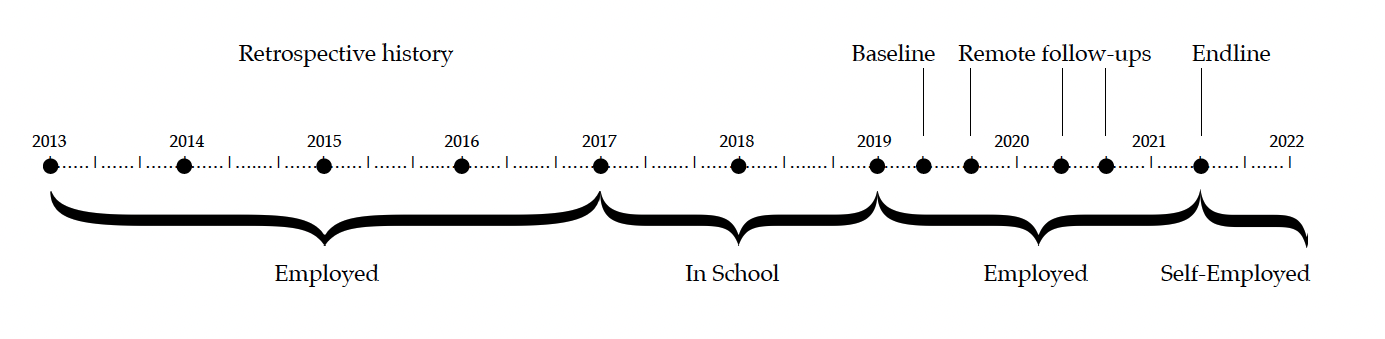
\includegraphics[width=1\textwidth]{figures/timeline}}
\end{figure}

The points indicate the dates at which youth are observed. This example individual was employed between 2013 and 2017, at which time she entered university. After two years at university, she returned to the labour market as a wage employee in early 2019, and continued to be wage employed for the majority of the period over which the survey was conducted. In the endline survey, she reported that she was no longer wage employed, and was instead supporting herself as a self-employed worker. These histories are used to study the SWT in the following three approaches.

\hypertarget{onset}{%
\subsubsection*{Graduation Age and Duration}\label{onset}}

First, we characterize the periods of school-leaving and labour market entry for the youth in the sample. As we can deduce the age of the respondent at each point of their observed employment history, we follow \textcite{manacorda2017} and calculate the age at which youth complete their schooling and transition to their first job and calculate the duration of this transition. We also draw on \textcite{bridges2017} and study youth employment status in the period directly after school-leaving. A wealth of socioeconomics and family characteristics allows us to identify factors that influence the time it takes for youth to enter the labour market.

We quantify four aspects of the SWT commonly studied in the literature: age at graduation or school-leaving, age at first employment, age at (permanent) labour market entry, and transition duration to first employment. The start of the SWT is often considered the point at which youth permanently leave school \autocite{bowers1998,nilsson2019}. Other definitions stipulate that only youth looking for work upon leaving school should be considered, in order to ensure that certain categories of youth, for instance women predisposed to domestic work, from skewing the unemployment numbers \autocite{matsumoto2010}. The ILO's \emph{Work4Youth} program takes school-leaving age to be the age of the onset of the SWT, as do several studies of the school-to-work transition in OECD countries (e.g. \textcite{bowers1998}, \textcite{quintini2007}). We take the age of youth at the time of their last observed period in school to be their \textbf{school-leaving age}. If youth are still in school at the time of the last interview, we assume that we have not observed their SWT and exclude them from these calculations.

Similarly, \textbf{age at first employment} is defined as the age at which youth first report being employed or self-employed, conditional on having spent at least one period in education or training in the past and not returning to school in subsequent periods. \textbf{Age at labour market entry} marks the first period for the same youth, but differs from first employment in that it excludes employment stints after which a return to schooling or training was observed. \textbf{School-leavers} are defined as youth for whom at least one period of schooling or training was observed, and whose last observed period was neither schooling nor training. Finally, we define the SWT \textbf{transition duration} as the difference between the age at school-leaving and the age at first employment\footnote{\hlc[pink]{Both cross-sectional and longitudinal data have been used to quantify the school-to-work transition in the literature. Cross-sectional data can be used to estimate the transition duration by subtracting the age at which 50 percent of  the  population  has  left  school  from  the  age  at  which  50  percent  of  the  population  has  found work. Quintini, J. P. Martin, and S. Martin (2007) and Quintini and S.Martin (2014) use this approach to report transition duration in advanced economies, along with mean school-leaving and first employment ages. For longitudinal studies,  the  mean  transition  duration,  reported  for  example  in  Quintini, J. P. Martin, and S. Martin (2007),  the  non-inclusion of youth still in transition will bias results.}}.

Youth for whom we cannot observe a first employment experience during the observation period or have already made the transition before the start of the observation period are considered to be right censored \autocite{nilsson2019}. In survival analysis, right-censored data refers event sequences where the exact event time of interest is unknown for some observations. Instead, the only information available is that the event has not occurred by the time the data were collected, or the event occurred after the end of the observation period. To estimate the duration of the transition using survival analysis, one can use a technique called survival function estimation, which involves modeling the probability of experiencing the event of interest (i.e., making the transition from school to work) as a function of time. We follow \textcite{nordman2015} and \textcite{manacorda2017} and use the non-parametric Kaplan-Meier estimator to approximate survival probabilities, i.e.~the probabilities that a youth needs an additional year to transition to the labour market after completing their schooling or training. \todo{8}

\hypertarget{markov}{%
\subsubsection*{Transitions as a Markov Process}\label{markov}}

A second empirical approach to studying labour market transitions is to interpret employment histories as a continuous Markov process between activity states or employment types \autocite{cunningham2011,bosch2007}. We construct transition matrices using the combined recall and survey data, which estimate the share of youth transitioning into or out of a given employment state over a specified period. This allows us to examine the flows between different activity states over the course of the SWT. Further, as outlined in \textcite{bosch2007}, we separate transition matrices into two discrete components: the propensity (to move) matrix, which represents transition probabilities independent of the rate of exit of any given subgroup from particular state, and the rate of separation matrix, which represents the overall rate of youth exiting from a given state (see Appendix \ref{markovapp} for a more detailed description). This allows us to understand whether the dynamics observed in the transition matrices are due to differences in entry and exit rates of young people into and from specific states or variations in turnover rates by age or gender.

Using the same event histories as before, we estimate transition matrices to understand the magnitude of turnover between various states over the course of the SWT. We estimate transition matrices for the entire sample, as well as propensity (to move) matrices for young men, women and different age brackets separately, to understand how transition dynamics differ by gender and change as youth get older.

\hypertarget{oma}{%
\subsubsection*{Optimal Matching Analysis}\label{oma}}

Third, we apply optimal matching analysis (OMA), a technique used to identify groups of similar states of sequences, to identify similarities in the SWT trajectories experienced by youth, and group them into clusters of similar transitions.

\todo{11}\hlc[lightgray]{OMA is a statistical technique that generates a measure of the similarity or difference between individual school-to-work transition sequences by comparing all pairs of sequences and performing insertions, deletions, or substitutions of single sequence elements to transform one sequence into the other} \autocite{elzinga2003}. Insertion and deletion costs are the cost of adding a new item to the sequence or removing an existing one, respectively, while the substitution cost is the cost of replacing one item in the sequence with another item\footnote{We use an insertion/deletion cost of 1 and a substitution cost matrix based on observed transition rates, which allows us to control for the likelihood of transitions occurring within the data.}. The resulting total cost required to change one sequence into another serves as a measure of similarity between all pairs of sequences. The distance matrix generated from this process is used in a hierarchical cluster analysis to group similar sequences into clusters: we use Ward's fusion algorithm to minimize within-group differences and maximize between-group differences \autocite{dlouhy2015,achatz2022}.

\todo{11}\hlc[lightgray]{This method has been used to study early career patterns in Italy, Great Britain, Sweden, and West Germany }\autocite{halpin1998,anyadike-danes2005,scherer2001,scherer2005,biemann2012,achatz2022}\hlc[lightgray]{. The method has also been applied to the school-to work transition in various high-income countries }\autocite{schoon2001,mcvicar2002,brzinsky-fay2007,brzinsky-fay2014,brzinsky-fay2016,middeldorp2019}. \textcite{quintini2009}\hlc[lightgray]{ use the method to compare school-to-work transitions between youth in the United States and Europe, and find considerably more dynamism in the US. One recent study has used Optimal Matching in a cross-country study of SWTs in low- and lower-middle income countries }\autocite{pesando2021}\hlc[lightgray]{, while the only other examples of OMA using data from LMICs are a study of the distance between experienced and ideal interpersonal relationships in Malawi }\autocite{frye2015}\hlc[lightgray]{, family planning (also in Malawi, }\textcite{furnas2016}\hlc[lightgray]{), and time usage among the elderly in South Africa }\autocite{grapsa2016}.

The TraMineR package in R \autocite{gabadinho2011} is used to perform the analysis, and the package WeightedCluster \autocite{studer2013} is used to compute various clustering quality measures to determine the optimal number of clusters. Finally, after identifying the clusters, we analyze how cluster membership is correlated to youth socioeconomic characteristics using logistic regression.

\hypertarget{survey-results}{%
\section{Results and Drivers}\label{survey-results}}

\hypertarget{survey-entry}{%
\subsection{Labour Market Entry}\label{survey-entry}}

We start by calculating transition statistics for youth who left school\footnote{The remainder were either in apprenticeship or schooling in the final observed period (and thus never transitioned to the labour market according to our definition) or were never in schooling or apprenticeship over the entirety of the period under observation and to whom the school-to-work transition does not apply (Manacorda, 2017).} over the observed period (7-year recall data and 3-year panel), shown in Table \ref{tab:tbl-entry}. A total of 471 youth, or 62 percent of the sample, finish school or training over the observed period; of these, we observe first employment spells for 451 youth (95.75 percent of observed school-leavers and 59.97 percent of the sample) and a labour market entry for 417 youth (88.54 of observed school-leavers and 55.45 percent of the sample). Half of the sample reports having their first employment experience by the age of 24, and 90 percent by the age of 27. Young men leave school about 7.5 months later than women, but require a comparable amount of time to find first employment. The mean school-leaving age is 22.62 years, with an average transition duration to labour market entry \todo{10}\hl{(defined as first employment stint without subsequent return to education or inactivity)} of just over one year.

\begin{singlespacing}
\begin{table}[H]

\caption{\label{tab:tbl-entry}Labour Market Entry}
\centering
\begin{threeparttable}
\fontsize{8}{10}\selectfont
\begin{tabular}[t]{l>{\centering\arraybackslash}p{4.5em}>{\centering\arraybackslash}p{4.5em}>{\centering\arraybackslash}p{4.5em}>{\centering\arraybackslash}p{4.5em}>{\centering\arraybackslash}p{4.5em}>{\centering\arraybackslash}p{4.5em}}
\toprule
\multicolumn{4}{c}{ } & \multicolumn{3}{c}{\makecell[c]{\textit{}Status in first \\period after school-leaving\textit{}}} \\
\cmidrule(l{3pt}r{3pt}){5-7}
\textbf{Characteristic} & \textbf{Overall} & \textbf{Female} (45\%) & \textbf{Male} (55\%) & \textbf{Employed} (38\%) & \textbf{NEET} (37\%) & \textbf{Self-}\newline \textbf{Employed} (24\%)\\
\midrule
N (observed school-leavers) & 471 & 213 & 258 & 181 & 176 & 114\\
Years of schooling & 14.32 (15) & 13.84 (15) & 14.72 (16) & 14.76 (16) & 14.49 (16) & 13.39 (14)\\
School-leaving age & 22.62 (23) & 22.27 (22) & 22.90 (23) & 22.66 (23) & 22.76 (23) & 22.33 (22)\\
Completed SWT (=1) & 89\% & 87\% & 90\% & 100\% & 69\% & 100\%\\
Age at labor market entry & 23.65 (24) & 23.36 (23) & 23.88 (24) & 23.47 (24) & 24.42 (24) & 23.11 (23)\\
Status at labor market entry &  &  &  &  &  & \\
\hspace{1em}Employed & 63\% & 59\% & 65\% & 100\% & 66\% & 0\%\\
\hspace{1em}Self-Employed & 37\% & 41\% & 35\% & 0\% & 34\% & 100\%\\
Duration of transition in years¹ & 1.06 (1) & 1.13 (1) & 1.01 (1) & 0.81 (1) & 1.70 (2) & 0.78 (1)\\
\bottomrule
\end{tabular}
\begin{tablenotes}
\item \textit{Notes:} Mean (median); \%.
\item[1] To labor market entry, defined as first work experience with no subsequent return to school or training.
\end{tablenotes}
\end{threeparttable}
\end{table}
\end{singlespacing}

The majority of school-leavers enter wage employment (38 percent) or self-employment (24 percent) directly after their last observed period of education or training. Youth who immediately enter self-employment are younger and completed fewer years of schooling compared to youth whose first post-schooling experience is wage employment or inactivity. Table \ref{tab:tbl-entry-full} in Appendix A3 shows that youth who immediately find wage employment are more often male and marry at a lower rate with fewer children (though only the difference for gender is significant). The self-employed also report the highest rate of completed apprenticeship and are generally less educated. Youth who experience a period of inactivity upon leaving school (i.e.~enter the labour market as NEET) have parents with slightly higher educational attainment, on average, than the parents of youth who immediately find work, consistent with the hypothesis that wealthy families are better able to support youth through extended periods of unemployment\footnote{\hlc[pink]{This contrasts with the findings of Bridges et al. (2017), who report the opposite: youth who enter the labour market as self-employed in Tanzania tend to have more educated parents.  This may be a result of differences in economic structure (Tanzania may have more opportunities for self-employment in sectors that require higher levels of education, such as professional services) or differences between the two countries in the cultural values attached to entrepreneurship.}}.

As nearly one sixth of our sample is still in school or training at endline, the data is right-censored and we expect the mean SWT transition to be downward biased. To address this, we apply survival analysis to the retrospective history data, following \textcite{nordman2015} and \textcite{manacorda2017}. Figure \ref{fig:fig-survival} in Appendix A3 plots the estimated survival probability: about 82 percent of youth need at least a year to transition to the labour market. Only about one percent of youth who transition report being unemployed for a period of four years or more. The adjustment for right-censored data does not significantly alter the estimated mean transition duration (SWT duration of 1.11 years after adjustment for right-censored data, compared to 1.06 years for the non-adjusted mean duration). After adjustment, we find that young men take 1.07 years to their first employment experience, while young women require 1.16 years, or about a month longer.

\todo{9}\hlc[pink]{How do our results for urban youth compare to the country as a whole? }\textcite{dedehouanou2019}\hlc[pink]{, using the 2014 SWTS, find that of a sample of individuals aged 15-29, 40 percent had transitioned to the labour market, with a median transition duration of 1.75 years (21 months). The median graduation age was 22 (23 in our sample) and the median first labour market experience was 25 (24 in our sample). The split of first job experience was 59:41 self-employment/salaried work, compared to the 63:37 split in our survey. While the authors find that men and women are similarly likely to exit the school-to-work transition (42 percent versus 38 percent, respectively), in our sample composed of older, urban youth this likelihood is much more skewed towards men (65 percent versus 47 percent).} This suggests that gender differences in transition rates are more pronounced in urban areas, and may be explained by higher levels of female labour in agriculture in rural areas in many low-income countries in SSA \autocite{croppenstedt2013} and the relative difficulty of young women to take advantage of the formal wage employment opportunities in urban labor markets \autocite{fox2012,fox2016}.

\todo{12}\hlc[pink]{Comparing our results with cross-country studies, we observe that the ages at which youth enter and exit the SWT in urban Bénin are closer to that of high-income countries than for the average youth in SSA. For instance, }\textcite{quintini2014} \hlc[pink]{report a median school-leaving age of between 21 and 22 years in a sample of advanced economies, compared to 17-18 in LMICs such as Brazil, India, Indonesia, Mexico and Turkey and 19-20 in selected Latin American countries (Argentina, Chile and South Africa). As their results are based on data over a decade old, this could also indicate a convergence in school-leaving age in recent years. Our results for SWT duration, on the other hand, are similar to the estimates of }\textcite{quintini2014}\hlc[pink]{ for LICs: the authors report that the duration of completed transitions is longer in emerging economies - 2.7 years for South Africa, and around 1 year for most LMICs, compared to 0.3-1.0 for HICs (except countries particularly affected by the Great Recession, such as Spain and Italy). }\textcite{manacorda2017}\hlc[pink]{, also using SWTS data from 23 lower-middle and lower income countries, report similar transition times to first employment as }\textcite{quintini2014}\hlc[pink]{ (25.7 months for SSA, 9.7 months for Bénin), but considerably longer transitions to permanent employment (11 year average for five countries in SSA, 2.6 years for Bénin). Our estimated transition duration for Bénin is considerably shorter than the SSA average reported in this study, however: 25.7 months to first employment and 129.7 months to steady employment}\footnote{Based on SWTS surveys from Bénin, Madagascar, Tanzania, Togo, Uganda.}.

\begin{singlespacing}

 \begin{table}[H] \centering    \caption{Transition Into First Employment}    \label{tab:tbl-firstempreg}  \scriptsize  \begin{tabular}{@{\extracolsep{3pt}}lcccc}  \\[-1.8ex]\hline  \hline \\[-1.8ex]  & & & \multicolumn{2}{c}{\underline{\shortstack{Status in first \\ period after school-leaving}}} \\   & \shortstack{Transition  \\ Age} & \shortstack{Transition \\ Duration} & \shortstack{NEET vs. \\ Wage} & \shortstack{Self vs. \\ Wage} \\  \\[-1.8ex] & (1) & (2) & (3) & (4)\\  \hline \\[-1.8ex]   Male (=1) & 0.55$^{**}$ & $-$0.08 & $-$0.50$^{**}$ & $-$0.24 \\    & (0.26) & (0.08) & (0.23) & (0.26) \\    Years of Schooling & $-$0.002 & $-$0.02 & $-$0.05 & $-$0.06 \\    & (0.06) & (0.02) & (0.05) & (0.06) \\    Completed apprenticeship (=1) & 0.30 & $-$0.13 & $-$0.47 & 0.19 \\    & (0.35) & (0.10) & (0.33) & (0.34) \\    Primary school diploma: CEP (=1) & $-$0.74 & 0.27 & $-$0.15 & 0.14 \\    & (0.58) & (0.17) & (0.54) & (0.57) \\    Junior high diploma: BEPC (=1) & 1.00$^{**}$ & 0.18 & 0.24 & $-$0.42 \\    & (0.43) & (0.13) & (0.39) & (0.42) \\    Baccalauréat: BAC (=1) & 0.66$^{*}$ & $-$0.18$^{*}$ & $-$0.33 & $-$0.02 \\    & (0.36) & (0.11) & (0.32) & (0.37) \\    Lower vocational: CAP (=1) & $-$0.23 & $-$0.05 & $-$0.28 & 0.22 \\    & (0.57) & (0.17) & (0.52) & (0.54) \\    2nd cycle university: Licence (=1) & 0.47 & 0.19$^{*}$ & 0.49 & 0.12 \\    & (0.38) & (0.11) & (0.32) & (0.40) \\    3rd cycle university: Maîtrise (=1) & 0.75 & 0.57$^{***}$ & 0.35 & 0.16 \\    & (0.71) & (0.21) & (0.62) & (0.78) \\    Father was apprentice (=1) & $-$0.24 & 0.07 & $-$0.12 & $-$0.27 \\    & (0.28) & (0.08) & (0.25) & (0.28) \\    Father completed primary (=1) & 0.65$^{**}$ & $-$0.03 & $-$0.36 & $-$0.38 \\    & (0.29) & (0.09) & (0.26) & (0.29) \\    Father completed secondary (=1) & $-$0.78$^{**}$ & 0.12 & 0.35 & $-$0.44 \\    & (0.39) & (0.12) & (0.34) & (0.42) \\    Mother was apprentice (=1) & 0.18 & $-$0.10 & 0.32 & 0.33 \\    & (0.34) & (0.10) & (0.31) & (0.35) \\    Mother completed primary (=1) & $-$0.36 & $-$0.005 & 0.31 & 0.65$^{*}$ \\    & (0.34) & (0.10) & (0.30) & (0.34) \\    Mother completed secondary (=1) & $-$0.35 & $-$0.26 & $-$0.38 & $-$0.02 \\    & (0.59) & (0.17) & (0.48) & (0.55) \\    Married (=1) & 0.29 & 0.36$^{***}$ & 0.36 & 0.25 \\    & (0.37) & (0.11) & (0.34) & (0.39) \\    Beninese (=1) & $-$0.86 & 0.04 & 0.55 & $-$0.003 \\    & (1.00) & (0.30) & (0.96) & (0.99) \\    Ethnicity: Fon (=1) & $-$0.28 & 0.01 & 0.22 & 0.65$^{**}$ \\    & (0.29) & (0.09) & (0.25) & (0.31) \\    Religion: Christian (=1) & 0.90$^{**}$ & 0.05 & $-$0.14 & $-$0.39 \\    & (0.36) & (0.11) & (0.33) & (0.36) \\    Grew up in a city (=1) & $-$0.03 & 0.09 & 0.28 & 0.77$^{***}$ \\    & (0.26) & (0.08) & (0.23) & (0.28) \\    Constant & 23.00$^{***}$ & 0.92$^{***}$ & 0.27 & 0.04 \\    & (1.10) & (0.34) & (1.10) & (1.10) \\   \hline \\[-1.8ex]  Observations & 417 & 417 & 471 & 471 \\  R$^{2}$ & 0.10 & 0.09 &  &  \\  Akaike Inf. Crit. &  &  & 1,048.00 & 1,048.00 \\  F Statistic & 2.30$^{***}$ & 1.90$^{**}$ &  &  \\  \hline  \hline \\[-1.8ex]  \multicolumn{5}{l}{$^{*}$p$<$0.1; $^{**}$p$<$0.05; $^{***}$p$<$0.01} \\  \end{tabular}  \end{table} 
\end{singlespacing}

\newpage

In a next step, we explore potential determinants of transition speed (age and duration) and employment status after school-leaving. We use OLS regression to estimate the effect of educational attainment and other socioeconomic characteristics on transition speed (Columns 1 and 2 of Table \ref{tab:tbl-firstempreg}), and a multinomial logit model to estimate the impact of the same variables on the probability that a youth becomes either wage employed, self-employed, or inactive (NEET) after leaving schooling or training.

The estimation results confirm that men enter the labour market about a half year later than women. The completion of secondary schooling (holding a junior high school diploma, BEPC, or a high school diploma, Baccalauréat) is associated with a later transition to the labour market, but does not affect the transition duration. Extended university education (Licence or higher), on the other hand, is associated with a longer transition: youth who have completed 3rd cycle university (master's level) take about six months longer to transition to the labour market. Youth with more educated fathers enter the labour market at a younger age: a possible reason being that youth whose fathers have higher levels of education may have access to better professional networks and resources that can help them find employment. Finally, the multinomial logit model estimates suggest that young men are less likely than young women to become NEET directly after leaving school, but we do not measure a significant effect of either youth education or parental education on the likelihood of finding employment in the first period after school-leaving.

\hypertarget{survey-paths}{%
\subsection{Transition Paths}\label{survey-paths}}

\hypertarget{transition-intensity-matrices}{%
\subsubsection*{Transition Intensity Matrices}\label{transition-intensity-matrices}}

\begin{figure}[H]
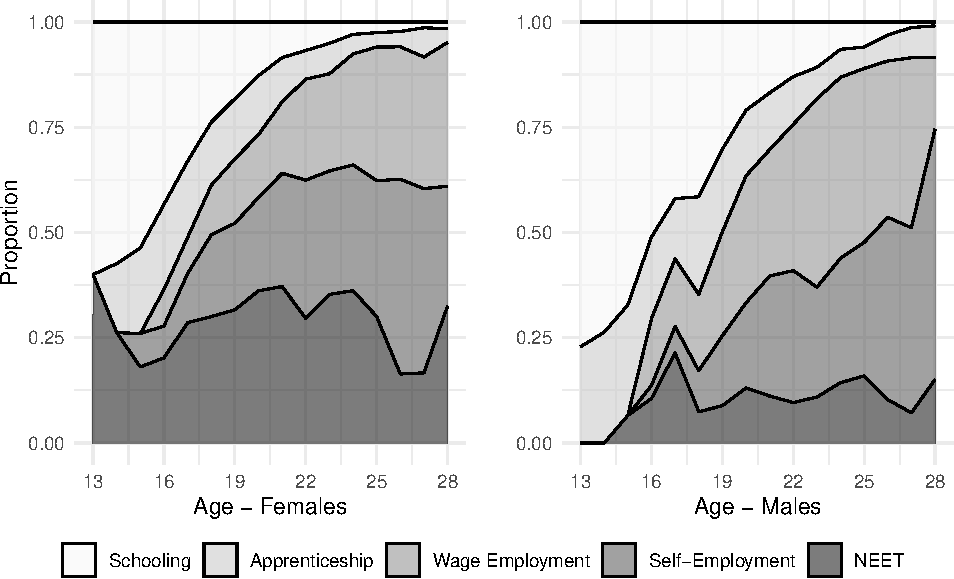
\includegraphics{figures/fig-ageplot-1} \caption{Activity status by age (combined survey and event history data)}\label{fig:fig-ageplot}
\end{figure}

In the following sections, we go beyond describing the transitions that bookend the SWT - school-leaving and labour market entry - and delve deeper into the dynamics of the SWT and flow between the five activity states by gender and age, depicted graphically in Figure \ref{fig:fig-ageplot}.

\begin{singlespacing}

\providecommand{\docline}[3]{\noalign{\global\setlength{\arrayrulewidth}{#1}}\arrayrulecolor[HTML]{#2}\cline{#3}}

\setlength{\tabcolsep}{0pt}

\renewcommand*{\arraystretch}{0.9}

\begin{longtable}[c]{|p{1.20in}|p{0.80in}|p{0.80in}|p{0.80in}|p{0.80in}|p{0.80in}}

\caption{\textcolor[HTML]{000000}{\fontsize{11}{13}\selectfont{\global\setmainfont{Palatino}{Activity\ transition\ matrix:\ Combined\ data,\ 2013-2021}}}}\label{tab:tbl-matrix}\\

\hhline{>{\arrayrulecolor[HTML]{000000}\global\arrayrulewidth=1pt}->{\arrayrulecolor[HTML]{000000}\global\arrayrulewidth=1pt}->{\arrayrulecolor[HTML]{000000}\global\arrayrulewidth=1pt}->{\arrayrulecolor[HTML]{000000}\global\arrayrulewidth=1pt}->{\arrayrulecolor[HTML]{000000}\global\arrayrulewidth=1pt}->{\arrayrulecolor[HTML]{000000}\global\arrayrulewidth=1pt}-}

\multicolumn{3}{!{\color[HTML]{FFFFFF}\vrule width 0pt}>{\centering}p{\dimexpr 2.8in+4\tabcolsep+2\arrayrulewidth}}{\textcolor[HTML]{000000}{\fontsize{9}{18}\selectfont{\global\setmainfont{Times New Roman}{}}}} & \multicolumn{3}{!{\color[HTML]{FFFFFF}\vrule width 0pt}>{\centering}p{\dimexpr 2.4in+4\tabcolsep+2\arrayrulewidth}!{\color[HTML]{FFFFFF}\vrule width 0pt}}{\textcolor[HTML]{000000}{\fontsize{9}{18}\selectfont{\global\setmainfont{Times New Roman}{To}}}} \\

\hhline{>{\arrayrulecolor[HTML]{000000}\global\arrayrulewidth=1pt}->{\arrayrulecolor[HTML]{000000}\global\arrayrulewidth=1pt}->{\arrayrulecolor[HTML]{000000}\global\arrayrulewidth=1pt}->{\arrayrulecolor[HTML]{000000}\global\arrayrulewidth=1pt}->{\arrayrulecolor[HTML]{000000}\global\arrayrulewidth=1pt}->{\arrayrulecolor[HTML]{000000}\global\arrayrulewidth=1pt}-}



\multicolumn{1}{!{\color[HTML]{FFFFFF}\vrule width 0pt}>{\centering}p{\dimexpr 1.2in+0\tabcolsep+0\arrayrulewidth}}{\textcolor[HTML]{000000}{\fontsize{9}{18}\selectfont{\global\setmainfont{Times New Roman}{From}}}} & \multicolumn{1}{!{\color[HTML]{FFFFFF}\vrule width 0pt}>{\centering}p{\dimexpr 0.8in+0\tabcolsep+0\arrayrulewidth}}{\textcolor[HTML]{000000}{\fontsize{9}{18}\selectfont{\global\setmainfont{Times New Roman}{In\ School}}}} & \multicolumn{1}{!{\color[HTML]{FFFFFF}\vrule width 0pt}>{\centering}p{\dimexpr 0.8in+0\tabcolsep+0\arrayrulewidth}}{\textcolor[HTML]{000000}{\fontsize{9}{18}\selectfont{\global\setmainfont{Times New Roman}{NEET}}}} & \multicolumn{1}{!{\color[HTML]{FFFFFF}\vrule width 0pt}>{\centering}p{\dimexpr 0.8in+0\tabcolsep+0\arrayrulewidth}}{\textcolor[HTML]{000000}{\fontsize{9}{18}\selectfont{\global\setmainfont{Times New Roman}{Self-Employed}}}} & \multicolumn{1}{!{\color[HTML]{FFFFFF}\vrule width 0pt}>{\centering}p{\dimexpr 0.8in+0\tabcolsep+0\arrayrulewidth}}{\textcolor[HTML]{000000}{\fontsize{9}{18}\selectfont{\global\setmainfont{Times New Roman}{Employed}}}} & \multicolumn{1}{!{\color[HTML]{FFFFFF}\vrule width 0pt}>{\centering}p{\dimexpr 0.8in+0\tabcolsep+0\arrayrulewidth}!{\color[HTML]{FFFFFF}\vrule width 0pt}}{\textcolor[HTML]{000000}{\fontsize{9}{18}\selectfont{\global\setmainfont{Times New Roman}{Apprentice}}}} \\

\hhline{>{\arrayrulecolor[HTML]{000000}\global\arrayrulewidth=1pt}->{\arrayrulecolor[HTML]{000000}\global\arrayrulewidth=1pt}->{\arrayrulecolor[HTML]{000000}\global\arrayrulewidth=1pt}->{\arrayrulecolor[HTML]{000000}\global\arrayrulewidth=1pt}->{\arrayrulecolor[HTML]{000000}\global\arrayrulewidth=1pt}->{\arrayrulecolor[HTML]{000000}\global\arrayrulewidth=1pt}-}\endhead



\multicolumn{6}{!{\color[HTML]{FFFFFF}\vrule width 0pt}>{\raggedright}p{\dimexpr 5.2in+10\tabcolsep+5\arrayrulewidth}!{\color[HTML]{FFFFFF}\vrule width 0pt}}{\textcolor[HTML]{000000}{\fontsize{9}{9}\selectfont{\global\setmainfont{Palatino}{\textit{Notes:\ }}}}\textcolor[HTML]{000000}{\fontsize{9}{9}\selectfont{\global\setmainfont{Palatino}{Row\ \%.\ First\ row\ for\ each\ activity\ refers\ to\ unconditional\ transition\ rate;\ remaining\ rates\ are\ conditional\ on\ the\ rate\ of\ separation.}}}} \\

\endfoot



\multicolumn{1}{!{\color[HTML]{FFFFFF}\vrule width 0pt}>{\raggedright}p{\dimexpr 1.2in+0\tabcolsep+0\arrayrulewidth}}{\textcolor[HTML]{000000}{\fontsize{9}{18}\selectfont{\global\setmainfont{Times New Roman}{\textbf{In\ School}}}}} & \multicolumn{1}{!{\color[HTML]{FFFFFF}\vrule width 0pt}>{\centering}p{\dimexpr 0.8in+0\tabcolsep+0\arrayrulewidth}}{\textcolor[HTML]{000000}{\fontsize{9}{18}\selectfont{\global\setmainfont{Times New Roman}{\textbf{85.68\%}}}}} & \multicolumn{1}{!{\color[HTML]{FFFFFF}\vrule width 0pt}>{\centering}p{\dimexpr 0.8in+0\tabcolsep+0\arrayrulewidth}}{\textcolor[HTML]{000000}{\fontsize{9}{18}\selectfont{\global\setmainfont{Times New Roman}{\textbf{3.85\%}}}}} & \multicolumn{1}{!{\color[HTML]{FFFFFF}\vrule width 0pt}>{\centering}p{\dimexpr 0.8in+0\tabcolsep+0\arrayrulewidth}}{\textcolor[HTML]{000000}{\fontsize{9}{18}\selectfont{\global\setmainfont{Times New Roman}{\textbf{2.61\%}}}}} & \multicolumn{1}{!{\color[HTML]{FFFFFF}\vrule width 0pt}>{\centering}p{\dimexpr 0.8in+0\tabcolsep+0\arrayrulewidth}}{\textcolor[HTML]{000000}{\fontsize{9}{18}\selectfont{\global\setmainfont{Times New Roman}{\textbf{4.92\%}}}}} & \multicolumn{1}{!{\color[HTML]{FFFFFF}\vrule width 0pt}>{\centering}p{\dimexpr 0.8in+0\tabcolsep+0\arrayrulewidth}!{\color[HTML]{FFFFFF}\vrule width 0pt}}{\textcolor[HTML]{000000}{\fontsize{9}{18}\selectfont{\global\setmainfont{Times New Roman}{\textbf{2.95\%}}}}} \\





\multicolumn{1}{!{\color[HTML]{FFFFFF}\vrule width 0pt}>{\raggedright}p{\dimexpr 1.2in+0\tabcolsep+0\arrayrulewidth}}{\textcolor[HTML]{000000}{\fontsize{9}{18}\selectfont{\global\setmainfont{Times New Roman}{Conditional}}}} & \multicolumn{1}{!{\color[HTML]{FFFFFF}\vrule width 0pt}>{\centering}p{\dimexpr 0.8in+0\tabcolsep+0\arrayrulewidth}}{\textcolor[HTML]{000000}{\fontsize{9}{18}\selectfont{\global\setmainfont{Times New Roman}{-}}}} & \multicolumn{1}{!{\color[HTML]{FFFFFF}\vrule width 0pt}>{\centering}p{\dimexpr 0.8in+0\tabcolsep+0\arrayrulewidth}}{\textcolor[HTML]{000000}{\fontsize{9}{18}\selectfont{\global\setmainfont{Times New Roman}{4.49\%}}}} & \multicolumn{1}{!{\color[HTML]{FFFFFF}\vrule width 0pt}>{\centering}p{\dimexpr 0.8in+0\tabcolsep+0\arrayrulewidth}}{\textcolor[HTML]{000000}{\fontsize{9}{18}\selectfont{\global\setmainfont{Times New Roman}{3.04\%}}}} & \multicolumn{1}{!{\color[HTML]{FFFFFF}\vrule width 0pt}>{\centering}p{\dimexpr 0.8in+0\tabcolsep+0\arrayrulewidth}}{\textcolor[HTML]{000000}{\fontsize{9}{18}\selectfont{\global\setmainfont{Times New Roman}{5.74\%}}}} & \multicolumn{1}{!{\color[HTML]{FFFFFF}\vrule width 0pt}>{\centering}p{\dimexpr 0.8in+0\tabcolsep+0\arrayrulewidth}!{\color[HTML]{FFFFFF}\vrule width 0pt}}{\textcolor[HTML]{000000}{\fontsize{9}{18}\selectfont{\global\setmainfont{Times New Roman}{3.44\%}}}} \\





\multicolumn{1}{!{\color[HTML]{FFFFFF}\vrule width 0pt}>{\raggedright}p{\dimexpr 1.2in+0\tabcolsep+0\arrayrulewidth}}{\textcolor[HTML]{000000}{\fontsize{9}{18}\selectfont{\global\setmainfont{Times New Roman}{Female}}}} & \multicolumn{1}{!{\color[HTML]{FFFFFF}\vrule width 0pt}>{\centering}p{\dimexpr 0.8in+0\tabcolsep+0\arrayrulewidth}}{\textcolor[HTML]{000000}{\fontsize{9}{18}\selectfont{\global\setmainfont{Times New Roman}{-}}}} & \multicolumn{1}{!{\color[HTML]{FFFFFF}\vrule width 0pt}>{\centering}p{\dimexpr 0.8in+0\tabcolsep+0\arrayrulewidth}}{\textcolor[HTML]{000000}{\fontsize{9}{18}\selectfont{\global\setmainfont{Times New Roman}{5.02\%}}}} & \multicolumn{1}{!{\color[HTML]{FFFFFF}\vrule width 0pt}>{\centering}p{\dimexpr 0.8in+0\tabcolsep+0\arrayrulewidth}}{\textcolor[HTML]{000000}{\fontsize{9}{18}\selectfont{\global\setmainfont{Times New Roman}{2.74\%}}}} & \multicolumn{1}{!{\color[HTML]{FFFFFF}\vrule width 0pt}>{\centering}p{\dimexpr 0.8in+0\tabcolsep+0\arrayrulewidth}}{\textcolor[HTML]{000000}{\fontsize{9}{18}\selectfont{\global\setmainfont{Times New Roman}{6.04\%}}}} & \multicolumn{1}{!{\color[HTML]{FFFFFF}\vrule width 0pt}>{\centering}p{\dimexpr 0.8in+0\tabcolsep+0\arrayrulewidth}!{\color[HTML]{FFFFFF}\vrule width 0pt}}{\textcolor[HTML]{000000}{\fontsize{9}{18}\selectfont{\global\setmainfont{Times New Roman}{4.45\%}}}} \\





\multicolumn{1}{!{\color[HTML]{FFFFFF}\vrule width 0pt}>{\raggedright}p{\dimexpr 1.2in+0\tabcolsep+0\arrayrulewidth}}{\textcolor[HTML]{000000}{\fontsize{9}{18}\selectfont{\global\setmainfont{Times New Roman}{Male}}}} & \multicolumn{1}{!{\color[HTML]{FFFFFF}\vrule width 0pt}>{\centering}p{\dimexpr 0.8in+0\tabcolsep+0\arrayrulewidth}}{\textcolor[HTML]{000000}{\fontsize{9}{18}\selectfont{\global\setmainfont{Times New Roman}{-}}}} & \multicolumn{1}{!{\color[HTML]{FFFFFF}\vrule width 0pt}>{\centering}p{\dimexpr 0.8in+0\tabcolsep+0\arrayrulewidth}}{\textcolor[HTML]{000000}{\fontsize{9}{18}\selectfont{\global\setmainfont{Times New Roman}{4.08\%}}}} & \multicolumn{1}{!{\color[HTML]{FFFFFF}\vrule width 0pt}>{\centering}p{\dimexpr 0.8in+0\tabcolsep+0\arrayrulewidth}}{\textcolor[HTML]{000000}{\fontsize{9}{18}\selectfont{\global\setmainfont{Times New Roman}{3.28\%}}}} & \multicolumn{1}{!{\color[HTML]{FFFFFF}\vrule width 0pt}>{\centering}p{\dimexpr 0.8in+0\tabcolsep+0\arrayrulewidth}}{\textcolor[HTML]{000000}{\fontsize{9}{18}\selectfont{\global\setmainfont{Times New Roman}{5.50\%}}}} & \multicolumn{1}{!{\color[HTML]{FFFFFF}\vrule width 0pt}>{\centering}p{\dimexpr 0.8in+0\tabcolsep+0\arrayrulewidth}!{\color[HTML]{FFFFFF}\vrule width 0pt}}{\textcolor[HTML]{000000}{\fontsize{9}{18}\selectfont{\global\setmainfont{Times New Roman}{2.66\%}}}} \\





\multicolumn{1}{!{\color[HTML]{FFFFFF}\vrule width 0pt}>{\raggedright}p{\dimexpr 1.2in+0\tabcolsep+0\arrayrulewidth}}{\textcolor[HTML]{000000}{\fontsize{9}{18}\selectfont{\global\setmainfont{Times New Roman}{14-18}}}} & \multicolumn{1}{!{\color[HTML]{FFFFFF}\vrule width 0pt}>{\centering}p{\dimexpr 0.8in+0\tabcolsep+0\arrayrulewidth}}{\textcolor[HTML]{000000}{\fontsize{9}{18}\selectfont{\global\setmainfont{Times New Roman}{-}}}} & \multicolumn{1}{!{\color[HTML]{FFFFFF}\vrule width 0pt}>{\centering}p{\dimexpr 0.8in+0\tabcolsep+0\arrayrulewidth}}{\textcolor[HTML]{000000}{\fontsize{9}{18}\selectfont{\global\setmainfont{Times New Roman}{1.32\%}}}} & \multicolumn{1}{!{\color[HTML]{FFFFFF}\vrule width 0pt}>{\centering}p{\dimexpr 0.8in+0\tabcolsep+0\arrayrulewidth}}{\textcolor[HTML]{000000}{\fontsize{9}{18}\selectfont{\global\setmainfont{Times New Roman}{1.08\%}}}} & \multicolumn{1}{!{\color[HTML]{FFFFFF}\vrule width 0pt}>{\centering}p{\dimexpr 0.8in+0\tabcolsep+0\arrayrulewidth}}{\textcolor[HTML]{000000}{\fontsize{9}{18}\selectfont{\global\setmainfont{Times New Roman}{0.96\%}}}} & \multicolumn{1}{!{\color[HTML]{FFFFFF}\vrule width 0pt}>{\centering}p{\dimexpr 0.8in+0\tabcolsep+0\arrayrulewidth}!{\color[HTML]{FFFFFF}\vrule width 0pt}}{\textcolor[HTML]{000000}{\fontsize{9}{18}\selectfont{\global\setmainfont{Times New Roman}{2.15\%}}}} \\





\multicolumn{1}{!{\color[HTML]{FFFFFF}\vrule width 0pt}>{\raggedright}p{\dimexpr 1.2in+0\tabcolsep+0\arrayrulewidth}}{\textcolor[HTML]{000000}{\fontsize{9}{18}\selectfont{\global\setmainfont{Times New Roman}{19-24}}}} & \multicolumn{1}{!{\color[HTML]{FFFFFF}\vrule width 0pt}>{\centering}p{\dimexpr 0.8in+0\tabcolsep+0\arrayrulewidth}}{\textcolor[HTML]{000000}{\fontsize{9}{18}\selectfont{\global\setmainfont{Times New Roman}{-}}}} & \multicolumn{1}{!{\color[HTML]{FFFFFF}\vrule width 0pt}>{\centering}p{\dimexpr 0.8in+0\tabcolsep+0\arrayrulewidth}}{\textcolor[HTML]{000000}{\fontsize{9}{18}\selectfont{\global\setmainfont{Times New Roman}{6.23\%}}}} & \multicolumn{1}{!{\color[HTML]{FFFFFF}\vrule width 0pt}>{\centering}p{\dimexpr 0.8in+0\tabcolsep+0\arrayrulewidth}}{\textcolor[HTML]{000000}{\fontsize{9}{18}\selectfont{\global\setmainfont{Times New Roman}{3.94\%}}}} & \multicolumn{1}{!{\color[HTML]{FFFFFF}\vrule width 0pt}>{\centering}p{\dimexpr 0.8in+0\tabcolsep+0\arrayrulewidth}}{\textcolor[HTML]{000000}{\fontsize{9}{18}\selectfont{\global\setmainfont{Times New Roman}{8.42\%}}}} & \multicolumn{1}{!{\color[HTML]{FFFFFF}\vrule width 0pt}>{\centering}p{\dimexpr 0.8in+0\tabcolsep+0\arrayrulewidth}!{\color[HTML]{FFFFFF}\vrule width 0pt}}{\textcolor[HTML]{000000}{\fontsize{9}{18}\selectfont{\global\setmainfont{Times New Roman}{4.40\%}}}} \\





\multicolumn{1}{!{\color[HTML]{FFFFFF}\vrule width 0pt}>{\raggedright}p{\dimexpr 1.2in+0\tabcolsep+0\arrayrulewidth}}{\textcolor[HTML]{000000}{\fontsize{9}{18}\selectfont{\global\setmainfont{Times New Roman}{25-30}}}} & \multicolumn{1}{!{\color[HTML]{FFFFFF}\vrule width 0pt}>{\centering}p{\dimexpr 0.8in+0\tabcolsep+0\arrayrulewidth}}{\textcolor[HTML]{000000}{\fontsize{9}{18}\selectfont{\global\setmainfont{Times New Roman}{-}}}} & \multicolumn{1}{!{\color[HTML]{FFFFFF}\vrule width 0pt}>{\centering}p{\dimexpr 0.8in+0\tabcolsep+0\arrayrulewidth}}{\textcolor[HTML]{000000}{\fontsize{9}{18}\selectfont{\global\setmainfont{Times New Roman}{14.47\%}}}} & \multicolumn{1}{!{\color[HTML]{FFFFFF}\vrule width 0pt}>{\centering}p{\dimexpr 0.8in+0\tabcolsep+0\arrayrulewidth}}{\textcolor[HTML]{000000}{\fontsize{9}{18}\selectfont{\global\setmainfont{Times New Roman}{11.84\%}}}} & \multicolumn{1}{!{\color[HTML]{FFFFFF}\vrule width 0pt}>{\centering}p{\dimexpr 0.8in+0\tabcolsep+0\arrayrulewidth}}{\textcolor[HTML]{000000}{\fontsize{9}{18}\selectfont{\global\setmainfont{Times New Roman}{19.74\%}}}} & \multicolumn{1}{!{\color[HTML]{FFFFFF}\vrule width 0pt}>{\centering}p{\dimexpr 0.8in+0\tabcolsep+0\arrayrulewidth}!{\color[HTML]{FFFFFF}\vrule width 0pt}}{\textcolor[HTML]{000000}{\fontsize{9}{18}\selectfont{\global\setmainfont{Times New Roman}{3.95\%}}}} \\





\multicolumn{1}{!{\color[HTML]{FFFFFF}\vrule width 0pt}>{\raggedright}p{\dimexpr 1.2in+0\tabcolsep+0\arrayrulewidth}}{\textcolor[HTML]{000000}{\fontsize{9}{18}\selectfont{\global\setmainfont{Times New Roman}{\textbf{NEET}}}}} & \multicolumn{1}{!{\color[HTML]{FFFFFF}\vrule width 0pt}>{\centering}p{\dimexpr 0.8in+0\tabcolsep+0\arrayrulewidth}}{\textcolor[HTML]{000000}{\fontsize{9}{18}\selectfont{\global\setmainfont{Times New Roman}{\textbf{1.82\%}}}}} & \multicolumn{1}{!{\color[HTML]{FFFFFF}\vrule width 0pt}>{\centering}p{\dimexpr 0.8in+0\tabcolsep+0\arrayrulewidth}}{\textcolor[HTML]{000000}{\fontsize{9}{18}\selectfont{\global\setmainfont{Times New Roman}{\textbf{64.94\%}}}}} & \multicolumn{1}{!{\color[HTML]{FFFFFF}\vrule width 0pt}>{\centering}p{\dimexpr 0.8in+0\tabcolsep+0\arrayrulewidth}}{\textcolor[HTML]{000000}{\fontsize{9}{18}\selectfont{\global\setmainfont{Times New Roman}{\textbf{11.17\%}}}}} & \multicolumn{1}{!{\color[HTML]{FFFFFF}\vrule width 0pt}>{\centering}p{\dimexpr 0.8in+0\tabcolsep+0\arrayrulewidth}}{\textcolor[HTML]{000000}{\fontsize{9}{18}\selectfont{\global\setmainfont{Times New Roman}{\textbf{14.29\%}}}}} & \multicolumn{1}{!{\color[HTML]{FFFFFF}\vrule width 0pt}>{\centering}p{\dimexpr 0.8in+0\tabcolsep+0\arrayrulewidth}!{\color[HTML]{FFFFFF}\vrule width 0pt}}{\textcolor[HTML]{000000}{\fontsize{9}{18}\selectfont{\global\setmainfont{Times New Roman}{\textbf{7.79\%}}}}} \\





\multicolumn{1}{!{\color[HTML]{FFFFFF}\vrule width 0pt}>{\raggedright}p{\dimexpr 1.2in+0\tabcolsep+0\arrayrulewidth}}{\textcolor[HTML]{000000}{\fontsize{9}{18}\selectfont{\global\setmainfont{Times New Roman}{Conditional}}}} & \multicolumn{1}{!{\color[HTML]{FFFFFF}\vrule width 0pt}>{\centering}p{\dimexpr 0.8in+0\tabcolsep+0\arrayrulewidth}}{\textcolor[HTML]{000000}{\fontsize{9}{18}\selectfont{\global\setmainfont{Times New Roman}{2.80\%}}}} & \multicolumn{1}{!{\color[HTML]{FFFFFF}\vrule width 0pt}>{\centering}p{\dimexpr 0.8in+0\tabcolsep+0\arrayrulewidth}}{\textcolor[HTML]{000000}{\fontsize{9}{18}\selectfont{\global\setmainfont{Times New Roman}{-}}}} & \multicolumn{1}{!{\color[HTML]{FFFFFF}\vrule width 0pt}>{\centering}p{\dimexpr 0.8in+0\tabcolsep+0\arrayrulewidth}}{\textcolor[HTML]{000000}{\fontsize{9}{18}\selectfont{\global\setmainfont{Times New Roman}{17.20\%}}}} & \multicolumn{1}{!{\color[HTML]{FFFFFF}\vrule width 0pt}>{\centering}p{\dimexpr 0.8in+0\tabcolsep+0\arrayrulewidth}}{\textcolor[HTML]{000000}{\fontsize{9}{18}\selectfont{\global\setmainfont{Times New Roman}{22.00\%}}}} & \multicolumn{1}{!{\color[HTML]{FFFFFF}\vrule width 0pt}>{\centering}p{\dimexpr 0.8in+0\tabcolsep+0\arrayrulewidth}!{\color[HTML]{FFFFFF}\vrule width 0pt}}{\textcolor[HTML]{000000}{\fontsize{9}{18}\selectfont{\global\setmainfont{Times New Roman}{12.00\%}}}} \\





\multicolumn{1}{!{\color[HTML]{FFFFFF}\vrule width 0pt}>{\raggedright}p{\dimexpr 1.2in+0\tabcolsep+0\arrayrulewidth}}{\textcolor[HTML]{000000}{\fontsize{9}{18}\selectfont{\global\setmainfont{Times New Roman}{Female}}}} & \multicolumn{1}{!{\color[HTML]{FFFFFF}\vrule width 0pt}>{\centering}p{\dimexpr 0.8in+0\tabcolsep+0\arrayrulewidth}}{\textcolor[HTML]{000000}{\fontsize{9}{18}\selectfont{\global\setmainfont{Times New Roman}{2.33\%}}}} & \multicolumn{1}{!{\color[HTML]{FFFFFF}\vrule width 0pt}>{\centering}p{\dimexpr 0.8in+0\tabcolsep+0\arrayrulewidth}}{\textcolor[HTML]{000000}{\fontsize{9}{18}\selectfont{\global\setmainfont{Times New Roman}{-}}}} & \multicolumn{1}{!{\color[HTML]{FFFFFF}\vrule width 0pt}>{\centering}p{\dimexpr 0.8in+0\tabcolsep+0\arrayrulewidth}}{\textcolor[HTML]{000000}{\fontsize{9}{18}\selectfont{\global\setmainfont{Times New Roman}{13.95\%}}}} & \multicolumn{1}{!{\color[HTML]{FFFFFF}\vrule width 0pt}>{\centering}p{\dimexpr 0.8in+0\tabcolsep+0\arrayrulewidth}}{\textcolor[HTML]{000000}{\fontsize{9}{18}\selectfont{\global\setmainfont{Times New Roman}{15.35\%}}}} & \multicolumn{1}{!{\color[HTML]{FFFFFF}\vrule width 0pt}>{\centering}p{\dimexpr 0.8in+0\tabcolsep+0\arrayrulewidth}!{\color[HTML]{FFFFFF}\vrule width 0pt}}{\textcolor[HTML]{000000}{\fontsize{9}{18}\selectfont{\global\setmainfont{Times New Roman}{7.91\%}}}} \\





\multicolumn{1}{!{\color[HTML]{FFFFFF}\vrule width 0pt}>{\raggedright}p{\dimexpr 1.2in+0\tabcolsep+0\arrayrulewidth}}{\textcolor[HTML]{000000}{\fontsize{9}{18}\selectfont{\global\setmainfont{Times New Roman}{Male}}}} & \multicolumn{1}{!{\color[HTML]{FFFFFF}\vrule width 0pt}>{\centering}p{\dimexpr 0.8in+0\tabcolsep+0\arrayrulewidth}}{\textcolor[HTML]{000000}{\fontsize{9}{18}\selectfont{\global\setmainfont{Times New Roman}{5.71\%}}}} & \multicolumn{1}{!{\color[HTML]{FFFFFF}\vrule width 0pt}>{\centering}p{\dimexpr 0.8in+0\tabcolsep+0\arrayrulewidth}}{\textcolor[HTML]{000000}{\fontsize{9}{18}\selectfont{\global\setmainfont{Times New Roman}{-}}}} & \multicolumn{1}{!{\color[HTML]{FFFFFF}\vrule width 0pt}>{\centering}p{\dimexpr 0.8in+0\tabcolsep+0\arrayrulewidth}}{\textcolor[HTML]{000000}{\fontsize{9}{18}\selectfont{\global\setmainfont{Times New Roman}{37.14\%}}}} & \multicolumn{1}{!{\color[HTML]{FFFFFF}\vrule width 0pt}>{\centering}p{\dimexpr 0.8in+0\tabcolsep+0\arrayrulewidth}}{\textcolor[HTML]{000000}{\fontsize{9}{18}\selectfont{\global\setmainfont{Times New Roman}{62.86\%}}}} & \multicolumn{1}{!{\color[HTML]{FFFFFF}\vrule width 0pt}>{\centering}p{\dimexpr 0.8in+0\tabcolsep+0\arrayrulewidth}!{\color[HTML]{FFFFFF}\vrule width 0pt}}{\textcolor[HTML]{000000}{\fontsize{9}{18}\selectfont{\global\setmainfont{Times New Roman}{37.14\%}}}} \\





\multicolumn{1}{!{\color[HTML]{FFFFFF}\vrule width 0pt}>{\raggedright}p{\dimexpr 1.2in+0\tabcolsep+0\arrayrulewidth}}{\textcolor[HTML]{000000}{\fontsize{9}{18}\selectfont{\global\setmainfont{Times New Roman}{14-18}}}} & \multicolumn{1}{!{\color[HTML]{FFFFFF}\vrule width 0pt}>{\centering}p{\dimexpr 0.8in+0\tabcolsep+0\arrayrulewidth}}{\textcolor[HTML]{000000}{\fontsize{9}{18}\selectfont{\global\setmainfont{Times New Roman}{4.76\%}}}} & \multicolumn{1}{!{\color[HTML]{FFFFFF}\vrule width 0pt}>{\centering}p{\dimexpr 0.8in+0\tabcolsep+0\arrayrulewidth}}{\textcolor[HTML]{000000}{\fontsize{9}{18}\selectfont{\global\setmainfont{Times New Roman}{-}}}} & \multicolumn{1}{!{\color[HTML]{FFFFFF}\vrule width 0pt}>{\centering}p{\dimexpr 0.8in+0\tabcolsep+0\arrayrulewidth}}{\textcolor[HTML]{000000}{\fontsize{9}{18}\selectfont{\global\setmainfont{Times New Roman}{7.14\%}}}} & \multicolumn{1}{!{\color[HTML]{FFFFFF}\vrule width 0pt}>{\centering}p{\dimexpr 0.8in+0\tabcolsep+0\arrayrulewidth}}{\textcolor[HTML]{000000}{\fontsize{9}{18}\selectfont{\global\setmainfont{Times New Roman}{11.90\%}}}} & \multicolumn{1}{!{\color[HTML]{FFFFFF}\vrule width 0pt}>{\centering}p{\dimexpr 0.8in+0\tabcolsep+0\arrayrulewidth}!{\color[HTML]{FFFFFF}\vrule width 0pt}}{\textcolor[HTML]{000000}{\fontsize{9}{18}\selectfont{\global\setmainfont{Times New Roman}{21.43\%}}}} \\





\multicolumn{1}{!{\color[HTML]{FFFFFF}\vrule width 0pt}>{\raggedright}p{\dimexpr 1.2in+0\tabcolsep+0\arrayrulewidth}}{\textcolor[HTML]{000000}{\fontsize{9}{18}\selectfont{\global\setmainfont{Times New Roman}{19-24}}}} & \multicolumn{1}{!{\color[HTML]{FFFFFF}\vrule width 0pt}>{\centering}p{\dimexpr 0.8in+0\tabcolsep+0\arrayrulewidth}}{\textcolor[HTML]{000000}{\fontsize{9}{18}\selectfont{\global\setmainfont{Times New Roman}{2.31\%}}}} & \multicolumn{1}{!{\color[HTML]{FFFFFF}\vrule width 0pt}>{\centering}p{\dimexpr 0.8in+0\tabcolsep+0\arrayrulewidth}}{\textcolor[HTML]{000000}{\fontsize{9}{18}\selectfont{\global\setmainfont{Times New Roman}{-}}}} & \multicolumn{1}{!{\color[HTML]{FFFFFF}\vrule width 0pt}>{\centering}p{\dimexpr 0.8in+0\tabcolsep+0\arrayrulewidth}}{\textcolor[HTML]{000000}{\fontsize{9}{18}\selectfont{\global\setmainfont{Times New Roman}{16.18\%}}}} & \multicolumn{1}{!{\color[HTML]{FFFFFF}\vrule width 0pt}>{\centering}p{\dimexpr 0.8in+0\tabcolsep+0\arrayrulewidth}}{\textcolor[HTML]{000000}{\fontsize{9}{18}\selectfont{\global\setmainfont{Times New Roman}{18.50\%}}}} & \multicolumn{1}{!{\color[HTML]{FFFFFF}\vrule width 0pt}>{\centering}p{\dimexpr 0.8in+0\tabcolsep+0\arrayrulewidth}!{\color[HTML]{FFFFFF}\vrule width 0pt}}{\textcolor[HTML]{000000}{\fontsize{9}{18}\selectfont{\global\setmainfont{Times New Roman}{9.83\%}}}} \\





\multicolumn{1}{!{\color[HTML]{FFFFFF}\vrule width 0pt}>{\raggedright}p{\dimexpr 1.2in+0\tabcolsep+0\arrayrulewidth}}{\textcolor[HTML]{000000}{\fontsize{9}{18}\selectfont{\global\setmainfont{Times New Roman}{25-30}}}} & \multicolumn{1}{!{\color[HTML]{FFFFFF}\vrule width 0pt}>{\centering}p{\dimexpr 0.8in+0\tabcolsep+0\arrayrulewidth}}{\textcolor[HTML]{000000}{\fontsize{9}{18}\selectfont{\global\setmainfont{Times New Roman}{2.86\%}}}} & \multicolumn{1}{!{\color[HTML]{FFFFFF}\vrule width 0pt}>{\centering}p{\dimexpr 0.8in+0\tabcolsep+0\arrayrulewidth}}{\textcolor[HTML]{000000}{\fontsize{9}{18}\selectfont{\global\setmainfont{Times New Roman}{-}}}} & \multicolumn{1}{!{\color[HTML]{FFFFFF}\vrule width 0pt}>{\centering}p{\dimexpr 0.8in+0\tabcolsep+0\arrayrulewidth}}{\textcolor[HTML]{000000}{\fontsize{9}{18}\selectfont{\global\setmainfont{Times New Roman}{34.29\%}}}} & \multicolumn{1}{!{\color[HTML]{FFFFFF}\vrule width 0pt}>{\centering}p{\dimexpr 0.8in+0\tabcolsep+0\arrayrulewidth}}{\textcolor[HTML]{000000}{\fontsize{9}{18}\selectfont{\global\setmainfont{Times New Roman}{51.43\%}}}} & \multicolumn{1}{!{\color[HTML]{FFFFFF}\vrule width 0pt}>{\centering}p{\dimexpr 0.8in+0\tabcolsep+0\arrayrulewidth}!{\color[HTML]{FFFFFF}\vrule width 0pt}}{\textcolor[HTML]{000000}{\fontsize{9}{18}\selectfont{\global\setmainfont{Times New Roman}{11.43\%}}}} \\





\multicolumn{1}{!{\color[HTML]{FFFFFF}\vrule width 0pt}>{\raggedright}p{\dimexpr 1.2in+0\tabcolsep+0\arrayrulewidth}}{\textcolor[HTML]{000000}{\fontsize{9}{18}\selectfont{\global\setmainfont{Times New Roman}{\textbf{Self-Employed}}}}} & \multicolumn{1}{!{\color[HTML]{FFFFFF}\vrule width 0pt}>{\centering}p{\dimexpr 0.8in+0\tabcolsep+0\arrayrulewidth}}{\textcolor[HTML]{000000}{\fontsize{9}{18}\selectfont{\global\setmainfont{Times New Roman}{\textbf{1.87\%}}}}} & \multicolumn{1}{!{\color[HTML]{FFFFFF}\vrule width 0pt}>{\centering}p{\dimexpr 0.8in+0\tabcolsep+0\arrayrulewidth}}{\textcolor[HTML]{000000}{\fontsize{9}{18}\selectfont{\global\setmainfont{Times New Roman}{\textbf{4.68\%}}}}} & \multicolumn{1}{!{\color[HTML]{FFFFFF}\vrule width 0pt}>{\centering}p{\dimexpr 0.8in+0\tabcolsep+0\arrayrulewidth}}{\textcolor[HTML]{000000}{\fontsize{9}{18}\selectfont{\global\setmainfont{Times New Roman}{\textbf{87.82\%}}}}} & \multicolumn{1}{!{\color[HTML]{FFFFFF}\vrule width 0pt}>{\centering}p{\dimexpr 0.8in+0\tabcolsep+0\arrayrulewidth}}{\textcolor[HTML]{000000}{\fontsize{9}{18}\selectfont{\global\setmainfont{Times New Roman}{\textbf{3.75\%}}}}} & \multicolumn{1}{!{\color[HTML]{FFFFFF}\vrule width 0pt}>{\centering}p{\dimexpr 0.8in+0\tabcolsep+0\arrayrulewidth}!{\color[HTML]{FFFFFF}\vrule width 0pt}}{\textcolor[HTML]{000000}{\fontsize{9}{18}\selectfont{\global\setmainfont{Times New Roman}{\textbf{1.87\%}}}}} \\





\multicolumn{1}{!{\color[HTML]{FFFFFF}\vrule width 0pt}>{\raggedright}p{\dimexpr 1.2in+0\tabcolsep+0\arrayrulewidth}}{\textcolor[HTML]{000000}{\fontsize{9}{18}\selectfont{\global\setmainfont{Times New Roman}{Conditional}}}} & \multicolumn{1}{!{\color[HTML]{FFFFFF}\vrule width 0pt}>{\centering}p{\dimexpr 0.8in+0\tabcolsep+0\arrayrulewidth}}{\textcolor[HTML]{000000}{\fontsize{9}{18}\selectfont{\global\setmainfont{Times New Roman}{2.13\%}}}} & \multicolumn{1}{!{\color[HTML]{FFFFFF}\vrule width 0pt}>{\centering}p{\dimexpr 0.8in+0\tabcolsep+0\arrayrulewidth}}{\textcolor[HTML]{000000}{\fontsize{9}{18}\selectfont{\global\setmainfont{Times New Roman}{5.33\%}}}} & \multicolumn{1}{!{\color[HTML]{FFFFFF}\vrule width 0pt}>{\centering}p{\dimexpr 0.8in+0\tabcolsep+0\arrayrulewidth}}{\textcolor[HTML]{000000}{\fontsize{9}{18}\selectfont{\global\setmainfont{Times New Roman}{-}}}} & \multicolumn{1}{!{\color[HTML]{FFFFFF}\vrule width 0pt}>{\centering}p{\dimexpr 0.8in+0\tabcolsep+0\arrayrulewidth}}{\textcolor[HTML]{000000}{\fontsize{9}{18}\selectfont{\global\setmainfont{Times New Roman}{4.27\%}}}} & \multicolumn{1}{!{\color[HTML]{FFFFFF}\vrule width 0pt}>{\centering}p{\dimexpr 0.8in+0\tabcolsep+0\arrayrulewidth}!{\color[HTML]{FFFFFF}\vrule width 0pt}}{\textcolor[HTML]{000000}{\fontsize{9}{18}\selectfont{\global\setmainfont{Times New Roman}{2.13\%}}}} \\





\multicolumn{1}{!{\color[HTML]{FFFFFF}\vrule width 0pt}>{\raggedright}p{\dimexpr 1.2in+0\tabcolsep+0\arrayrulewidth}}{\textcolor[HTML]{000000}{\fontsize{9}{18}\selectfont{\global\setmainfont{Times New Roman}{Female}}}} & \multicolumn{1}{!{\color[HTML]{FFFFFF}\vrule width 0pt}>{\centering}p{\dimexpr 0.8in+0\tabcolsep+0\arrayrulewidth}}{\textcolor[HTML]{000000}{\fontsize{9}{18}\selectfont{\global\setmainfont{Times New Roman}{0.96\%}}}} & \multicolumn{1}{!{\color[HTML]{FFFFFF}\vrule width 0pt}>{\centering}p{\dimexpr 0.8in+0\tabcolsep+0\arrayrulewidth}}{\textcolor[HTML]{000000}{\fontsize{9}{18}\selectfont{\global\setmainfont{Times New Roman}{6.22\%}}}} & \multicolumn{1}{!{\color[HTML]{FFFFFF}\vrule width 0pt}>{\centering}p{\dimexpr 0.8in+0\tabcolsep+0\arrayrulewidth}}{\textcolor[HTML]{000000}{\fontsize{9}{18}\selectfont{\global\setmainfont{Times New Roman}{-}}}} & \multicolumn{1}{!{\color[HTML]{FFFFFF}\vrule width 0pt}>{\centering}p{\dimexpr 0.8in+0\tabcolsep+0\arrayrulewidth}}{\textcolor[HTML]{000000}{\fontsize{9}{18}\selectfont{\global\setmainfont{Times New Roman}{4.31\%}}}} & \multicolumn{1}{!{\color[HTML]{FFFFFF}\vrule width 0pt}>{\centering}p{\dimexpr 0.8in+0\tabcolsep+0\arrayrulewidth}!{\color[HTML]{FFFFFF}\vrule width 0pt}}{\textcolor[HTML]{000000}{\fontsize{9}{18}\selectfont{\global\setmainfont{Times New Roman}{2.87\%}}}} \\





\multicolumn{1}{!{\color[HTML]{FFFFFF}\vrule width 0pt}>{\raggedright}p{\dimexpr 1.2in+0\tabcolsep+0\arrayrulewidth}}{\textcolor[HTML]{000000}{\fontsize{9}{18}\selectfont{\global\setmainfont{Times New Roman}{Male}}}} & \multicolumn{1}{!{\color[HTML]{FFFFFF}\vrule width 0pt}>{\centering}p{\dimexpr 0.8in+0\tabcolsep+0\arrayrulewidth}}{\textcolor[HTML]{000000}{\fontsize{9}{18}\selectfont{\global\setmainfont{Times New Roman}{3.61\%}}}} & \multicolumn{1}{!{\color[HTML]{FFFFFF}\vrule width 0pt}>{\centering}p{\dimexpr 0.8in+0\tabcolsep+0\arrayrulewidth}}{\textcolor[HTML]{000000}{\fontsize{9}{18}\selectfont{\global\setmainfont{Times New Roman}{4.22\%}}}} & \multicolumn{1}{!{\color[HTML]{FFFFFF}\vrule width 0pt}>{\centering}p{\dimexpr 0.8in+0\tabcolsep+0\arrayrulewidth}}{\textcolor[HTML]{000000}{\fontsize{9}{18}\selectfont{\global\setmainfont{Times New Roman}{-}}}} & \multicolumn{1}{!{\color[HTML]{FFFFFF}\vrule width 0pt}>{\centering}p{\dimexpr 0.8in+0\tabcolsep+0\arrayrulewidth}}{\textcolor[HTML]{000000}{\fontsize{9}{18}\selectfont{\global\setmainfont{Times New Roman}{4.22\%}}}} & \multicolumn{1}{!{\color[HTML]{FFFFFF}\vrule width 0pt}>{\centering}p{\dimexpr 0.8in+0\tabcolsep+0\arrayrulewidth}!{\color[HTML]{FFFFFF}\vrule width 0pt}}{\textcolor[HTML]{000000}{\fontsize{9}{18}\selectfont{\global\setmainfont{Times New Roman}{1.20\%}}}} \\





\multicolumn{1}{!{\color[HTML]{FFFFFF}\vrule width 0pt}>{\raggedright}p{\dimexpr 1.2in+0\tabcolsep+0\arrayrulewidth}}{\textcolor[HTML]{000000}{\fontsize{9}{18}\selectfont{\global\setmainfont{Times New Roman}{14-18}}}} & \multicolumn{1}{!{\color[HTML]{FFFFFF}\vrule width 0pt}>{\centering}p{\dimexpr 0.8in+0\tabcolsep+0\arrayrulewidth}}{\textcolor[HTML]{000000}{\fontsize{9}{18}\selectfont{\global\setmainfont{Times New Roman}{0.00\%}}}} & \multicolumn{1}{!{\color[HTML]{FFFFFF}\vrule width 0pt}>{\centering}p{\dimexpr 0.8in+0\tabcolsep+0\arrayrulewidth}}{\textcolor[HTML]{000000}{\fontsize{9}{18}\selectfont{\global\setmainfont{Times New Roman}{0.00\%}}}} & \multicolumn{1}{!{\color[HTML]{FFFFFF}\vrule width 0pt}>{\centering}p{\dimexpr 0.8in+0\tabcolsep+0\arrayrulewidth}}{\textcolor[HTML]{000000}{\fontsize{9}{18}\selectfont{\global\setmainfont{Times New Roman}{-}}}} & \multicolumn{1}{!{\color[HTML]{FFFFFF}\vrule width 0pt}>{\centering}p{\dimexpr 0.8in+0\tabcolsep+0\arrayrulewidth}}{\textcolor[HTML]{000000}{\fontsize{9}{18}\selectfont{\global\setmainfont{Times New Roman}{0.00\%}}}} & \multicolumn{1}{!{\color[HTML]{FFFFFF}\vrule width 0pt}>{\centering}p{\dimexpr 0.8in+0\tabcolsep+0\arrayrulewidth}!{\color[HTML]{FFFFFF}\vrule width 0pt}}{\textcolor[HTML]{000000}{\fontsize{9}{18}\selectfont{\global\setmainfont{Times New Roman}{14.29\%}}}} \\





\multicolumn{1}{!{\color[HTML]{FFFFFF}\vrule width 0pt}>{\raggedright}p{\dimexpr 1.2in+0\tabcolsep+0\arrayrulewidth}}{\textcolor[HTML]{000000}{\fontsize{9}{18}\selectfont{\global\setmainfont{Times New Roman}{19-24}}}} & \multicolumn{1}{!{\color[HTML]{FFFFFF}\vrule width 0pt}>{\centering}p{\dimexpr 0.8in+0\tabcolsep+0\arrayrulewidth}}{\textcolor[HTML]{000000}{\fontsize{9}{18}\selectfont{\global\setmainfont{Times New Roman}{2.90\%}}}} & \multicolumn{1}{!{\color[HTML]{FFFFFF}\vrule width 0pt}>{\centering}p{\dimexpr 0.8in+0\tabcolsep+0\arrayrulewidth}}{\textcolor[HTML]{000000}{\fontsize{9}{18}\selectfont{\global\setmainfont{Times New Roman}{6.22\%}}}} & \multicolumn{1}{!{\color[HTML]{FFFFFF}\vrule width 0pt}>{\centering}p{\dimexpr 0.8in+0\tabcolsep+0\arrayrulewidth}}{\textcolor[HTML]{000000}{\fontsize{9}{18}\selectfont{\global\setmainfont{Times New Roman}{-}}}} & \multicolumn{1}{!{\color[HTML]{FFFFFF}\vrule width 0pt}>{\centering}p{\dimexpr 0.8in+0\tabcolsep+0\arrayrulewidth}}{\textcolor[HTML]{000000}{\fontsize{9}{18}\selectfont{\global\setmainfont{Times New Roman}{5.39\%}}}} & \multicolumn{1}{!{\color[HTML]{FFFFFF}\vrule width 0pt}>{\centering}p{\dimexpr 0.8in+0\tabcolsep+0\arrayrulewidth}!{\color[HTML]{FFFFFF}\vrule width 0pt}}{\textcolor[HTML]{000000}{\fontsize{9}{18}\selectfont{\global\setmainfont{Times New Roman}{1.66\%}}}} \\





\multicolumn{1}{!{\color[HTML]{FFFFFF}\vrule width 0pt}>{\raggedright}p{\dimexpr 1.2in+0\tabcolsep+0\arrayrulewidth}}{\textcolor[HTML]{000000}{\fontsize{9}{18}\selectfont{\global\setmainfont{Times New Roman}{25-30}}}} & \multicolumn{1}{!{\color[HTML]{FFFFFF}\vrule width 0pt}>{\centering}p{\dimexpr 0.8in+0\tabcolsep+0\arrayrulewidth}}{\textcolor[HTML]{000000}{\fontsize{9}{18}\selectfont{\global\setmainfont{Times New Roman}{0.83\%}}}} & \multicolumn{1}{!{\color[HTML]{FFFFFF}\vrule width 0pt}>{\centering}p{\dimexpr 0.8in+0\tabcolsep+0\arrayrulewidth}}{\textcolor[HTML]{000000}{\fontsize{9}{18}\selectfont{\global\setmainfont{Times New Roman}{4.17\%}}}} & \multicolumn{1}{!{\color[HTML]{FFFFFF}\vrule width 0pt}>{\centering}p{\dimexpr 0.8in+0\tabcolsep+0\arrayrulewidth}}{\textcolor[HTML]{000000}{\fontsize{9}{18}\selectfont{\global\setmainfont{Times New Roman}{-}}}} & \multicolumn{1}{!{\color[HTML]{FFFFFF}\vrule width 0pt}>{\centering}p{\dimexpr 0.8in+0\tabcolsep+0\arrayrulewidth}}{\textcolor[HTML]{000000}{\fontsize{9}{18}\selectfont{\global\setmainfont{Times New Roman}{2.50\%}}}} & \multicolumn{1}{!{\color[HTML]{FFFFFF}\vrule width 0pt}>{\centering}p{\dimexpr 0.8in+0\tabcolsep+0\arrayrulewidth}!{\color[HTML]{FFFFFF}\vrule width 0pt}}{\textcolor[HTML]{000000}{\fontsize{9}{18}\selectfont{\global\setmainfont{Times New Roman}{1.67\%}}}} \\





\multicolumn{1}{!{\color[HTML]{FFFFFF}\vrule width 0pt}>{\raggedright}p{\dimexpr 1.2in+0\tabcolsep+0\arrayrulewidth}}{\textcolor[HTML]{000000}{\fontsize{9}{18}\selectfont{\global\setmainfont{Times New Roman}{\textbf{Employed}}}}} & \multicolumn{1}{!{\color[HTML]{FFFFFF}\vrule width 0pt}>{\centering}p{\dimexpr 0.8in+0\tabcolsep+0\arrayrulewidth}}{\textcolor[HTML]{000000}{\fontsize{9}{18}\selectfont{\global\setmainfont{Times New Roman}{\textbf{1.28\%}}}}} & \multicolumn{1}{!{\color[HTML]{FFFFFF}\vrule width 0pt}>{\centering}p{\dimexpr 0.8in+0\tabcolsep+0\arrayrulewidth}}{\textcolor[HTML]{000000}{\fontsize{9}{18}\selectfont{\global\setmainfont{Times New Roman}{\textbf{7.23\%}}}}} & \multicolumn{1}{!{\color[HTML]{FFFFFF}\vrule width 0pt}>{\centering}p{\dimexpr 0.8in+0\tabcolsep+0\arrayrulewidth}}{\textcolor[HTML]{000000}{\fontsize{9}{18}\selectfont{\global\setmainfont{Times New Roman}{\textbf{4.68\%}}}}} & \multicolumn{1}{!{\color[HTML]{FFFFFF}\vrule width 0pt}>{\centering}p{\dimexpr 0.8in+0\tabcolsep+0\arrayrulewidth}}{\textcolor[HTML]{000000}{\fontsize{9}{18}\selectfont{\global\setmainfont{Times New Roman}{\textbf{84.89\%}}}}} & \multicolumn{1}{!{\color[HTML]{FFFFFF}\vrule width 0pt}>{\centering}p{\dimexpr 0.8in+0\tabcolsep+0\arrayrulewidth}!{\color[HTML]{FFFFFF}\vrule width 0pt}}{\textcolor[HTML]{000000}{\fontsize{9}{18}\selectfont{\global\setmainfont{Times New Roman}{\textbf{1.91\%}}}}} \\





\multicolumn{1}{!{\color[HTML]{FFFFFF}\vrule width 0pt}>{\raggedright}p{\dimexpr 1.2in+0\tabcolsep+0\arrayrulewidth}}{\textcolor[HTML]{000000}{\fontsize{9}{18}\selectfont{\global\setmainfont{Times New Roman}{Conditional}}}} & \multicolumn{1}{!{\color[HTML]{FFFFFF}\vrule width 0pt}>{\centering}p{\dimexpr 0.8in+0\tabcolsep+0\arrayrulewidth}}{\textcolor[HTML]{000000}{\fontsize{9}{18}\selectfont{\global\setmainfont{Times New Roman}{1.50\%}}}} & \multicolumn{1}{!{\color[HTML]{FFFFFF}\vrule width 0pt}>{\centering}p{\dimexpr 0.8in+0\tabcolsep+0\arrayrulewidth}}{\textcolor[HTML]{000000}{\fontsize{9}{18}\selectfont{\global\setmainfont{Times New Roman}{8.52\%}}}} & \multicolumn{1}{!{\color[HTML]{FFFFFF}\vrule width 0pt}>{\centering}p{\dimexpr 0.8in+0\tabcolsep+0\arrayrulewidth}}{\textcolor[HTML]{000000}{\fontsize{9}{18}\selectfont{\global\setmainfont{Times New Roman}{5.51\%}}}} & \multicolumn{1}{!{\color[HTML]{FFFFFF}\vrule width 0pt}>{\centering}p{\dimexpr 0.8in+0\tabcolsep+0\arrayrulewidth}}{\textcolor[HTML]{000000}{\fontsize{9}{18}\selectfont{\global\setmainfont{Times New Roman}{-}}}} & \multicolumn{1}{!{\color[HTML]{FFFFFF}\vrule width 0pt}>{\centering}p{\dimexpr 0.8in+0\tabcolsep+0\arrayrulewidth}!{\color[HTML]{FFFFFF}\vrule width 0pt}}{\textcolor[HTML]{000000}{\fontsize{9}{18}\selectfont{\global\setmainfont{Times New Roman}{2.26\%}}}} \\





\multicolumn{1}{!{\color[HTML]{FFFFFF}\vrule width 0pt}>{\raggedright}p{\dimexpr 1.2in+0\tabcolsep+0\arrayrulewidth}}{\textcolor[HTML]{000000}{\fontsize{9}{18}\selectfont{\global\setmainfont{Times New Roman}{Female}}}} & \multicolumn{1}{!{\color[HTML]{FFFFFF}\vrule width 0pt}>{\centering}p{\dimexpr 0.8in+0\tabcolsep+0\arrayrulewidth}}{\textcolor[HTML]{000000}{\fontsize{9}{18}\selectfont{\global\setmainfont{Times New Roman}{2.00\%}}}} & \multicolumn{1}{!{\color[HTML]{FFFFFF}\vrule width 0pt}>{\centering}p{\dimexpr 0.8in+0\tabcolsep+0\arrayrulewidth}}{\textcolor[HTML]{000000}{\fontsize{9}{18}\selectfont{\global\setmainfont{Times New Roman}{18.00\%}}}} & \multicolumn{1}{!{\color[HTML]{FFFFFF}\vrule width 0pt}>{\centering}p{\dimexpr 0.8in+0\tabcolsep+0\arrayrulewidth}}{\textcolor[HTML]{000000}{\fontsize{9}{18}\selectfont{\global\setmainfont{Times New Roman}{5.33\%}}}} & \multicolumn{1}{!{\color[HTML]{FFFFFF}\vrule width 0pt}>{\centering}p{\dimexpr 0.8in+0\tabcolsep+0\arrayrulewidth}}{\textcolor[HTML]{000000}{\fontsize{9}{18}\selectfont{\global\setmainfont{Times New Roman}{-}}}} & \multicolumn{1}{!{\color[HTML]{FFFFFF}\vrule width 0pt}>{\centering}p{\dimexpr 0.8in+0\tabcolsep+0\arrayrulewidth}!{\color[HTML]{FFFFFF}\vrule width 0pt}}{\textcolor[HTML]{000000}{\fontsize{9}{18}\selectfont{\global\setmainfont{Times New Roman}{2.67\%}}}} \\





\multicolumn{1}{!{\color[HTML]{FFFFFF}\vrule width 0pt}>{\raggedright}p{\dimexpr 1.2in+0\tabcolsep+0\arrayrulewidth}}{\textcolor[HTML]{000000}{\fontsize{9}{18}\selectfont{\global\setmainfont{Times New Roman}{Male}}}} & \multicolumn{1}{!{\color[HTML]{FFFFFF}\vrule width 0pt}>{\centering}p{\dimexpr 0.8in+0\tabcolsep+0\arrayrulewidth}}{\textcolor[HTML]{000000}{\fontsize{9}{18}\selectfont{\global\setmainfont{Times New Roman}{1.20\%}}}} & \multicolumn{1}{!{\color[HTML]{FFFFFF}\vrule width 0pt}>{\centering}p{\dimexpr 0.8in+0\tabcolsep+0\arrayrulewidth}}{\textcolor[HTML]{000000}{\fontsize{9}{18}\selectfont{\global\setmainfont{Times New Roman}{2.81\%}}}} & \multicolumn{1}{!{\color[HTML]{FFFFFF}\vrule width 0pt}>{\centering}p{\dimexpr 0.8in+0\tabcolsep+0\arrayrulewidth}}{\textcolor[HTML]{000000}{\fontsize{9}{18}\selectfont{\global\setmainfont{Times New Roman}{5.62\%}}}} & \multicolumn{1}{!{\color[HTML]{FFFFFF}\vrule width 0pt}>{\centering}p{\dimexpr 0.8in+0\tabcolsep+0\arrayrulewidth}}{\textcolor[HTML]{000000}{\fontsize{9}{18}\selectfont{\global\setmainfont{Times New Roman}{-}}}} & \multicolumn{1}{!{\color[HTML]{FFFFFF}\vrule width 0pt}>{\centering}p{\dimexpr 0.8in+0\tabcolsep+0\arrayrulewidth}!{\color[HTML]{FFFFFF}\vrule width 0pt}}{\textcolor[HTML]{000000}{\fontsize{9}{18}\selectfont{\global\setmainfont{Times New Roman}{2.01\%}}}} \\





\multicolumn{1}{!{\color[HTML]{FFFFFF}\vrule width 0pt}>{\raggedright}p{\dimexpr 1.2in+0\tabcolsep+0\arrayrulewidth}}{\textcolor[HTML]{000000}{\fontsize{9}{18}\selectfont{\global\setmainfont{Times New Roman}{14-18}}}} & \multicolumn{1}{!{\color[HTML]{FFFFFF}\vrule width 0pt}>{\centering}p{\dimexpr 0.8in+0\tabcolsep+0\arrayrulewidth}}{\textcolor[HTML]{000000}{\fontsize{9}{18}\selectfont{\global\setmainfont{Times New Roman}{5.00\%}}}} & \multicolumn{1}{!{\color[HTML]{FFFFFF}\vrule width 0pt}>{\centering}p{\dimexpr 0.8in+0\tabcolsep+0\arrayrulewidth}}{\textcolor[HTML]{000000}{\fontsize{9}{18}\selectfont{\global\setmainfont{Times New Roman}{10.00\%}}}} & \multicolumn{1}{!{\color[HTML]{FFFFFF}\vrule width 0pt}>{\centering}p{\dimexpr 0.8in+0\tabcolsep+0\arrayrulewidth}}{\textcolor[HTML]{000000}{\fontsize{9}{18}\selectfont{\global\setmainfont{Times New Roman}{10.00\%}}}} & \multicolumn{1}{!{\color[HTML]{FFFFFF}\vrule width 0pt}>{\centering}p{\dimexpr 0.8in+0\tabcolsep+0\arrayrulewidth}}{\textcolor[HTML]{000000}{\fontsize{9}{18}\selectfont{\global\setmainfont{Times New Roman}{-}}}} & \multicolumn{1}{!{\color[HTML]{FFFFFF}\vrule width 0pt}>{\centering}p{\dimexpr 0.8in+0\tabcolsep+0\arrayrulewidth}!{\color[HTML]{FFFFFF}\vrule width 0pt}}{\textcolor[HTML]{000000}{\fontsize{9}{18}\selectfont{\global\setmainfont{Times New Roman}{0.00\%}}}} \\





\multicolumn{1}{!{\color[HTML]{FFFFFF}\vrule width 0pt}>{\raggedright}p{\dimexpr 1.2in+0\tabcolsep+0\arrayrulewidth}}{\textcolor[HTML]{000000}{\fontsize{9}{18}\selectfont{\global\setmainfont{Times New Roman}{19-24}}}} & \multicolumn{1}{!{\color[HTML]{FFFFFF}\vrule width 0pt}>{\centering}p{\dimexpr 0.8in+0\tabcolsep+0\arrayrulewidth}}{\textcolor[HTML]{000000}{\fontsize{9}{18}\selectfont{\global\setmainfont{Times New Roman}{1.53\%}}}} & \multicolumn{1}{!{\color[HTML]{FFFFFF}\vrule width 0pt}>{\centering}p{\dimexpr 0.8in+0\tabcolsep+0\arrayrulewidth}}{\textcolor[HTML]{000000}{\fontsize{9}{18}\selectfont{\global\setmainfont{Times New Roman}{8.78\%}}}} & \multicolumn{1}{!{\color[HTML]{FFFFFF}\vrule width 0pt}>{\centering}p{\dimexpr 0.8in+0\tabcolsep+0\arrayrulewidth}}{\textcolor[HTML]{000000}{\fontsize{9}{18}\selectfont{\global\setmainfont{Times New Roman}{6.49\%}}}} & \multicolumn{1}{!{\color[HTML]{FFFFFF}\vrule width 0pt}>{\centering}p{\dimexpr 0.8in+0\tabcolsep+0\arrayrulewidth}}{\textcolor[HTML]{000000}{\fontsize{9}{18}\selectfont{\global\setmainfont{Times New Roman}{-}}}} & \multicolumn{1}{!{\color[HTML]{FFFFFF}\vrule width 0pt}>{\centering}p{\dimexpr 0.8in+0\tabcolsep+0\arrayrulewidth}!{\color[HTML]{FFFFFF}\vrule width 0pt}}{\textcolor[HTML]{000000}{\fontsize{9}{18}\selectfont{\global\setmainfont{Times New Roman}{3.05\%}}}} \\





\multicolumn{1}{!{\color[HTML]{FFFFFF}\vrule width 0pt}>{\raggedright}p{\dimexpr 1.2in+0\tabcolsep+0\arrayrulewidth}}{\textcolor[HTML]{000000}{\fontsize{9}{18}\selectfont{\global\setmainfont{Times New Roman}{25-30}}}} & \multicolumn{1}{!{\color[HTML]{FFFFFF}\vrule width 0pt}>{\centering}p{\dimexpr 0.8in+0\tabcolsep+0\arrayrulewidth}}{\textcolor[HTML]{000000}{\fontsize{9}{18}\selectfont{\global\setmainfont{Times New Roman}{0.85\%}}}} & \multicolumn{1}{!{\color[HTML]{FFFFFF}\vrule width 0pt}>{\centering}p{\dimexpr 0.8in+0\tabcolsep+0\arrayrulewidth}}{\textcolor[HTML]{000000}{\fontsize{9}{18}\selectfont{\global\setmainfont{Times New Roman}{7.69\%}}}} & \multicolumn{1}{!{\color[HTML]{FFFFFF}\vrule width 0pt}>{\centering}p{\dimexpr 0.8in+0\tabcolsep+0\arrayrulewidth}}{\textcolor[HTML]{000000}{\fontsize{9}{18}\selectfont{\global\setmainfont{Times New Roman}{2.56\%}}}} & \multicolumn{1}{!{\color[HTML]{FFFFFF}\vrule width 0pt}>{\centering}p{\dimexpr 0.8in+0\tabcolsep+0\arrayrulewidth}}{\textcolor[HTML]{000000}{\fontsize{9}{18}\selectfont{\global\setmainfont{Times New Roman}{-}}}} & \multicolumn{1}{!{\color[HTML]{FFFFFF}\vrule width 0pt}>{\centering}p{\dimexpr 0.8in+0\tabcolsep+0\arrayrulewidth}!{\color[HTML]{FFFFFF}\vrule width 0pt}}{\textcolor[HTML]{000000}{\fontsize{9}{18}\selectfont{\global\setmainfont{Times New Roman}{0.85\%}}}} \\





\multicolumn{1}{!{\color[HTML]{FFFFFF}\vrule width 0pt}>{\raggedright}p{\dimexpr 1.2in+0\tabcolsep+0\arrayrulewidth}}{\textcolor[HTML]{000000}{\fontsize{9}{18}\selectfont{\global\setmainfont{Times New Roman}{\textbf{Apprentice}}}}} & \multicolumn{1}{!{\color[HTML]{FFFFFF}\vrule width 0pt}>{\centering}p{\dimexpr 0.8in+0\tabcolsep+0\arrayrulewidth}}{\textcolor[HTML]{000000}{\fontsize{9}{18}\selectfont{\global\setmainfont{Times New Roman}{\textbf{0.26\%}}}}} & \multicolumn{1}{!{\color[HTML]{FFFFFF}\vrule width 0pt}>{\centering}p{\dimexpr 0.8in+0\tabcolsep+0\arrayrulewidth}}{\textcolor[HTML]{000000}{\fontsize{9}{18}\selectfont{\global\setmainfont{Times New Roman}{\textbf{5.25\%}}}}} & \multicolumn{1}{!{\color[HTML]{FFFFFF}\vrule width 0pt}>{\centering}p{\dimexpr 0.8in+0\tabcolsep+0\arrayrulewidth}}{\textcolor[HTML]{000000}{\fontsize{9}{18}\selectfont{\global\setmainfont{Times New Roman}{\textbf{9.45\%}}}}} & \multicolumn{1}{!{\color[HTML]{FFFFFF}\vrule width 0pt}>{\centering}p{\dimexpr 0.8in+0\tabcolsep+0\arrayrulewidth}}{\textcolor[HTML]{000000}{\fontsize{9}{18}\selectfont{\global\setmainfont{Times New Roman}{\textbf{10.50\%}}}}} & \multicolumn{1}{!{\color[HTML]{FFFFFF}\vrule width 0pt}>{\centering}p{\dimexpr 0.8in+0\tabcolsep+0\arrayrulewidth}!{\color[HTML]{FFFFFF}\vrule width 0pt}}{\textcolor[HTML]{000000}{\fontsize{9}{18}\selectfont{\global\setmainfont{Times New Roman}{\textbf{74.54\%}}}}} \\





\multicolumn{1}{!{\color[HTML]{FFFFFF}\vrule width 0pt}>{\raggedright}p{\dimexpr 1.2in+0\tabcolsep+0\arrayrulewidth}}{\textcolor[HTML]{000000}{\fontsize{9}{18}\selectfont{\global\setmainfont{Times New Roman}{Conditional}}}} & \multicolumn{1}{!{\color[HTML]{FFFFFF}\vrule width 0pt}>{\centering}p{\dimexpr 0.8in+0\tabcolsep+0\arrayrulewidth}}{\textcolor[HTML]{000000}{\fontsize{9}{18}\selectfont{\global\setmainfont{Times New Roman}{0.35\%}}}} & \multicolumn{1}{!{\color[HTML]{FFFFFF}\vrule width 0pt}>{\centering}p{\dimexpr 0.8in+0\tabcolsep+0\arrayrulewidth}}{\textcolor[HTML]{000000}{\fontsize{9}{18}\selectfont{\global\setmainfont{Times New Roman}{7.04\%}}}} & \multicolumn{1}{!{\color[HTML]{FFFFFF}\vrule width 0pt}>{\centering}p{\dimexpr 0.8in+0\tabcolsep+0\arrayrulewidth}}{\textcolor[HTML]{000000}{\fontsize{9}{18}\selectfont{\global\setmainfont{Times New Roman}{12.68\%}}}} & \multicolumn{1}{!{\color[HTML]{FFFFFF}\vrule width 0pt}>{\centering}p{\dimexpr 0.8in+0\tabcolsep+0\arrayrulewidth}}{\textcolor[HTML]{000000}{\fontsize{9}{18}\selectfont{\global\setmainfont{Times New Roman}{14.08\%}}}} & \multicolumn{1}{!{\color[HTML]{FFFFFF}\vrule width 0pt}>{\centering}p{\dimexpr 0.8in+0\tabcolsep+0\arrayrulewidth}!{\color[HTML]{FFFFFF}\vrule width 0pt}}{\textcolor[HTML]{000000}{\fontsize{9}{18}\selectfont{\global\setmainfont{Times New Roman}{-}}}} \\





\multicolumn{1}{!{\color[HTML]{FFFFFF}\vrule width 0pt}>{\raggedright}p{\dimexpr 1.2in+0\tabcolsep+0\arrayrulewidth}}{\textcolor[HTML]{000000}{\fontsize{9}{18}\selectfont{\global\setmainfont{Times New Roman}{Female}}}} & \multicolumn{1}{!{\color[HTML]{FFFFFF}\vrule width 0pt}>{\centering}p{\dimexpr 0.8in+0\tabcolsep+0\arrayrulewidth}}{\textcolor[HTML]{000000}{\fontsize{9}{18}\selectfont{\global\setmainfont{Times New Roman}{0.00\%}}}} & \multicolumn{1}{!{\color[HTML]{FFFFFF}\vrule width 0pt}>{\centering}p{\dimexpr 0.8in+0\tabcolsep+0\arrayrulewidth}}{\textcolor[HTML]{000000}{\fontsize{9}{18}\selectfont{\global\setmainfont{Times New Roman}{11.36\%}}}} & \multicolumn{1}{!{\color[HTML]{FFFFFF}\vrule width 0pt}>{\centering}p{\dimexpr 0.8in+0\tabcolsep+0\arrayrulewidth}}{\textcolor[HTML]{000000}{\fontsize{9}{18}\selectfont{\global\setmainfont{Times New Roman}{13.64\%}}}} & \multicolumn{1}{!{\color[HTML]{FFFFFF}\vrule width 0pt}>{\centering}p{\dimexpr 0.8in+0\tabcolsep+0\arrayrulewidth}}{\textcolor[HTML]{000000}{\fontsize{9}{18}\selectfont{\global\setmainfont{Times New Roman}{12.88\%}}}} & \multicolumn{1}{!{\color[HTML]{FFFFFF}\vrule width 0pt}>{\centering}p{\dimexpr 0.8in+0\tabcolsep+0\arrayrulewidth}!{\color[HTML]{FFFFFF}\vrule width 0pt}}{\textcolor[HTML]{000000}{\fontsize{9}{18}\selectfont{\global\setmainfont{Times New Roman}{-}}}} \\





\multicolumn{1}{!{\color[HTML]{FFFFFF}\vrule width 0pt}>{\raggedright}p{\dimexpr 1.2in+0\tabcolsep+0\arrayrulewidth}}{\textcolor[HTML]{000000}{\fontsize{9}{18}\selectfont{\global\setmainfont{Times New Roman}{Male}}}} & \multicolumn{1}{!{\color[HTML]{FFFFFF}\vrule width 0pt}>{\centering}p{\dimexpr 0.8in+0\tabcolsep+0\arrayrulewidth}}{\textcolor[HTML]{000000}{\fontsize{9}{18}\selectfont{\global\setmainfont{Times New Roman}{0.66\%}}}} & \multicolumn{1}{!{\color[HTML]{FFFFFF}\vrule width 0pt}>{\centering}p{\dimexpr 0.8in+0\tabcolsep+0\arrayrulewidth}}{\textcolor[HTML]{000000}{\fontsize{9}{18}\selectfont{\global\setmainfont{Times New Roman}{3.29\%}}}} & \multicolumn{1}{!{\color[HTML]{FFFFFF}\vrule width 0pt}>{\centering}p{\dimexpr 0.8in+0\tabcolsep+0\arrayrulewidth}}{\textcolor[HTML]{000000}{\fontsize{9}{18}\selectfont{\global\setmainfont{Times New Roman}{11.84\%}}}} & \multicolumn{1}{!{\color[HTML]{FFFFFF}\vrule width 0pt}>{\centering}p{\dimexpr 0.8in+0\tabcolsep+0\arrayrulewidth}}{\textcolor[HTML]{000000}{\fontsize{9}{18}\selectfont{\global\setmainfont{Times New Roman}{15.13\%}}}} & \multicolumn{1}{!{\color[HTML]{FFFFFF}\vrule width 0pt}>{\centering}p{\dimexpr 0.8in+0\tabcolsep+0\arrayrulewidth}!{\color[HTML]{FFFFFF}\vrule width 0pt}}{\textcolor[HTML]{000000}{\fontsize{9}{18}\selectfont{\global\setmainfont{Times New Roman}{-}}}} \\





\multicolumn{1}{!{\color[HTML]{FFFFFF}\vrule width 0pt}>{\raggedright}p{\dimexpr 1.2in+0\tabcolsep+0\arrayrulewidth}}{\textcolor[HTML]{000000}{\fontsize{9}{18}\selectfont{\global\setmainfont{Times New Roman}{14-18}}}} & \multicolumn{1}{!{\color[HTML]{FFFFFF}\vrule width 0pt}>{\centering}p{\dimexpr 0.8in+0\tabcolsep+0\arrayrulewidth}}{\textcolor[HTML]{000000}{\fontsize{9}{18}\selectfont{\global\setmainfont{Times New Roman}{0.00\%}}}} & \multicolumn{1}{!{\color[HTML]{FFFFFF}\vrule width 0pt}>{\centering}p{\dimexpr 0.8in+0\tabcolsep+0\arrayrulewidth}}{\textcolor[HTML]{000000}{\fontsize{9}{18}\selectfont{\global\setmainfont{Times New Roman}{3.90\%}}}} & \multicolumn{1}{!{\color[HTML]{FFFFFF}\vrule width 0pt}>{\centering}p{\dimexpr 0.8in+0\tabcolsep+0\arrayrulewidth}}{\textcolor[HTML]{000000}{\fontsize{9}{18}\selectfont{\global\setmainfont{Times New Roman}{2.60\%}}}} & \multicolumn{1}{!{\color[HTML]{FFFFFF}\vrule width 0pt}>{\centering}p{\dimexpr 0.8in+0\tabcolsep+0\arrayrulewidth}}{\textcolor[HTML]{000000}{\fontsize{9}{18}\selectfont{\global\setmainfont{Times New Roman}{3.90\%}}}} & \multicolumn{1}{!{\color[HTML]{FFFFFF}\vrule width 0pt}>{\centering}p{\dimexpr 0.8in+0\tabcolsep+0\arrayrulewidth}!{\color[HTML]{FFFFFF}\vrule width 0pt}}{\textcolor[HTML]{000000}{\fontsize{9}{18}\selectfont{\global\setmainfont{Times New Roman}{-}}}} \\





\multicolumn{1}{!{\color[HTML]{FFFFFF}\vrule width 0pt}>{\raggedright}p{\dimexpr 1.2in+0\tabcolsep+0\arrayrulewidth}}{\textcolor[HTML]{000000}{\fontsize{9}{18}\selectfont{\global\setmainfont{Times New Roman}{19-24}}}} & \multicolumn{1}{!{\color[HTML]{FFFFFF}\vrule width 0pt}>{\centering}p{\dimexpr 0.8in+0\tabcolsep+0\arrayrulewidth}}{\textcolor[HTML]{000000}{\fontsize{9}{18}\selectfont{\global\setmainfont{Times New Roman}{0.00\%}}}} & \multicolumn{1}{!{\color[HTML]{FFFFFF}\vrule width 0pt}>{\centering}p{\dimexpr 0.8in+0\tabcolsep+0\arrayrulewidth}}{\textcolor[HTML]{000000}{\fontsize{9}{18}\selectfont{\global\setmainfont{Times New Roman}{8.20\%}}}} & \multicolumn{1}{!{\color[HTML]{FFFFFF}\vrule width 0pt}>{\centering}p{\dimexpr 0.8in+0\tabcolsep+0\arrayrulewidth}}{\textcolor[HTML]{000000}{\fontsize{9}{18}\selectfont{\global\setmainfont{Times New Roman}{14.75\%}}}} & \multicolumn{1}{!{\color[HTML]{FFFFFF}\vrule width 0pt}>{\centering}p{\dimexpr 0.8in+0\tabcolsep+0\arrayrulewidth}}{\textcolor[HTML]{000000}{\fontsize{9}{18}\selectfont{\global\setmainfont{Times New Roman}{18.58\%}}}} & \multicolumn{1}{!{\color[HTML]{FFFFFF}\vrule width 0pt}>{\centering}p{\dimexpr 0.8in+0\tabcolsep+0\arrayrulewidth}!{\color[HTML]{FFFFFF}\vrule width 0pt}}{\textcolor[HTML]{000000}{\fontsize{9}{18}\selectfont{\global\setmainfont{Times New Roman}{-}}}} \\





\multicolumn{1}{!{\color[HTML]{FFFFFF}\vrule width 0pt}>{\raggedright}p{\dimexpr 1.2in+0\tabcolsep+0\arrayrulewidth}}{\textcolor[HTML]{000000}{\fontsize{9}{18}\selectfont{\global\setmainfont{Times New Roman}{25-30}}}} & \multicolumn{1}{!{\color[HTML]{FFFFFF}\vrule width 0pt}>{\centering}p{\dimexpr 0.8in+0\tabcolsep+0\arrayrulewidth}}{\textcolor[HTML]{000000}{\fontsize{9}{18}\selectfont{\global\setmainfont{Times New Roman}{4.17\%}}}} & \multicolumn{1}{!{\color[HTML]{FFFFFF}\vrule width 0pt}>{\centering}p{\dimexpr 0.8in+0\tabcolsep+0\arrayrulewidth}}{\textcolor[HTML]{000000}{\fontsize{9}{18}\selectfont{\global\setmainfont{Times New Roman}{8.33\%}}}} & \multicolumn{1}{!{\color[HTML]{FFFFFF}\vrule width 0pt}>{\centering}p{\dimexpr 0.8in+0\tabcolsep+0\arrayrulewidth}}{\textcolor[HTML]{000000}{\fontsize{9}{18}\selectfont{\global\setmainfont{Times New Roman}{29.17\%}}}} & \multicolumn{1}{!{\color[HTML]{FFFFFF}\vrule width 0pt}>{\centering}p{\dimexpr 0.8in+0\tabcolsep+0\arrayrulewidth}}{\textcolor[HTML]{000000}{\fontsize{9}{18}\selectfont{\global\setmainfont{Times New Roman}{12.50\%}}}} & \multicolumn{1}{!{\color[HTML]{FFFFFF}\vrule width 0pt}>{\centering}p{\dimexpr 0.8in+0\tabcolsep+0\arrayrulewidth}!{\color[HTML]{FFFFFF}\vrule width 0pt}}{\textcolor[HTML]{000000}{\fontsize{9}{18}\selectfont{\global\setmainfont{Times New Roman}{-}}}} \\

\hhline{>{\arrayrulecolor[HTML]{000000}\global\arrayrulewidth=1pt}->{\arrayrulecolor[HTML]{000000}\global\arrayrulewidth=1pt}->{\arrayrulecolor[HTML]{000000}\global\arrayrulewidth=1pt}->{\arrayrulecolor[HTML]{000000}\global\arrayrulewidth=1pt}->{\arrayrulecolor[HTML]{000000}\global\arrayrulewidth=1pt}->{\arrayrulecolor[HTML]{000000}\global\arrayrulewidth=1pt}-}



\end{longtable}
\end{singlespacing}

Table \ref{tab:tbl-matrix} reports transition rates into activity states using pooled recall history and survey data from the entire observation period. Rows represent the initial state and columns the final state, and the percentages in each cell represent the probability of an individual transitioning from the initial to the final state (i.e.~the state in the subsequent period). The first row of each state reports the unconditional transition rate, equivalent to the raw percentage of youth transitioning between two activities as a percentage of youth in the initial state. This frequency alone, however, does not allow us to make any inference about the relative desirability of a change, as it does not control for the inherent tendency to ``separate'' from the activity \autocite{bosch2010}. For instance, few youth leave schooling when compared to NEET: thus, comparing raw transition rates to employment between the two activities will not reflect the relative disposition of youth to enter employment directly from the two initial states (see Appendix \ref{markov} for more details). Hence, the rates from estimated propensity matrices are reported in the remaining rows, which standardize the rates on the probability of separation - first for the entire sample, and then by gender and age subgroups.

Overall, Table \ref{tab:tbl-matrix} reflects the broad contours one would expect from the SWT: youth aged 18-24 are relatively unlikely to transition out of schooling or training; as they age, they enter the labour market as self-employed, employed, or NEET at increasing rates. Apprentices -- especially older ones -- are more likely to transition to self-employment than wage employment. The rates at which youth exit NEET status and find work, particularly wage employment, increase dramatically as youth age. The inverse is also true of the wage employed: the probability that they exit employment in one period and enter NEET status in the next falls for older age subgroups. Table \ref{tab:tbl-matrix} also reveals stark gender differences in transition patterns. Females are more likely to change states to NEET, regardless of the initial state, and less likely to transition from NEET once inactive. The gaps in the conditional transition rate from employment to NEET (18 percent for women, 2.8 percent for men), from NEET to self-employment (14 percent versus 37.1 percent, respectively) and NEET to wage employment (15 percent versus 62.9 percent) are particularly pronounced.

We note that transitions to wage employment (from either school or apprenticeship training) are more frequent than to self-employment. While this may be expected for schooling, which intuitively increases the likelihood of finding a wage job, it is less expected for apprentices. One explanation may be that apprentices continue working for their former master trainer (or another employer) upon school-leaving in order to save up the capital needed to start their own business.

Transition matrices are presented separately for the event history data and the panel data, as well as the transitions between all rounds of the panel survey, in Appendix B2. On average, 39.7 percent of youth changed activities between each survey round, a much higher rate than the 17 percent observed in the event history data, reflecting both the higher instability associated with the transition phase (compared to school-age years) and, potentially, more frequent variation in youth activity, particularly after school-leaving, than can be captured by annual data.

\hypertarget{optimal-matching-analysis}{%
\subsubsection*{Optimal Matching Analysis}\label{optimal-matching-analysis}}

\begin{figure}[H]
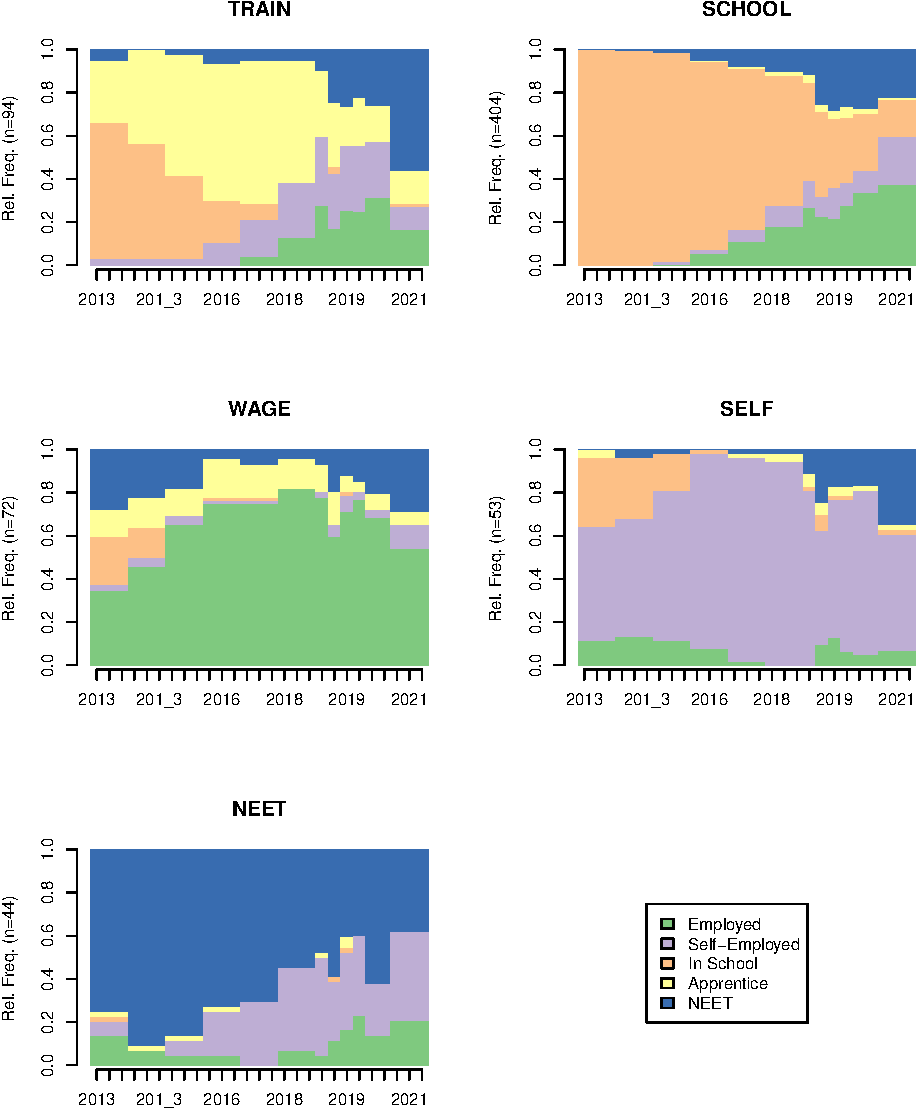
\includegraphics{figures/fig-clusters-1} \caption{Occupational status distribution plots by cluster}\label{fig:fig-clusters}
\end{figure}

Next, we employ Optimal Matching Analysis (OMA) to identify clusters of youth following similar paths during their school-to-work transition. Figure \ref{fig:fig-clusters} plots the five identified clusters of youth transition resulting from minimizing Optimal Matching distances. In examining the figures, we note that the clusters correspond closely to the five base activity states; we label them TRAIN, SCHOOL, WAGE, SELF and NEET for simplicity. Descriptive statistics for each cluster are presented in Table \ref{tab:tbl-clustertbl}, while a logistic regression on cluster membership with the usual socio-economic characteristics as covariates is presented Table \ref{tab:tbl-clusterreg}, both in Appendix A3.

The first cluster, TRAIN, is the most heterogeneous, and includes many transitions from school to apprenticeship and from apprenticeship into the three labour market states (NEET, wage employment and self-employment). It is primarily comprised of youth who participated in apprenticeship training in the years leading up to the baseline survey. Youth begin to transition into wage employment, self-employment, or inactivity in roughly equal proportions in around 2018, with a considerable proportion shifting to inactivity at endline. As apprenticeship training is generally considered to be a reliable route to (informal sector) employment, this shift to inactivity is concerning and may be a issue to be addressed with labor market integration policies. The youth in this cluster completed about 9 years of school, with the majority dropping out before completing junior high school.

The second cluster, SCHOOL, accounts for about 60 percent of the sample, and is dominated by formal education, especially in the period leading up to the baseline survey. These trajectories are clearly oriented towards transition into wage employment, with a pronounced increase of NEET youth at the time of the baseline survey. This increase in NEET youth may be explained either by under-reporting of NEET periods in the recall data, a sharp increase in economic inactivity during the Covid-19 pandemic, or the higher frequency and granularity of the panel survey relative to the event history data. Despite the high educational attainment of this group (14.9 years on average, by far the most of any cluster), the relative frequency of NEET status is the lowest of any of the five clusters, indicating that over-education is not an issue for youth in following this trajectory. This cluster is characterised by relatively low marriage and childbearing rates, and logistic regression on cluster membership (Table \ref{tab:tbl-clusterreg} in Appendix A3) also reveals higher parental education of the youth in this cluster.

The third cluster, WAGE, is comprised of 72 youth who are primarily engaged in wage employment over the observed period. Most of these youth had completed their formal education by the beginning of the observation period and enjoyed fairly stable employment throughout -- with a small proportion transitioning to inactivity at the start of the panel survey, again signalling potential under-reporting of NEET status or worsening economic conditions during the pandemic. Estimates from our logistic regression suggest that males are more likely to follow the WAGE trajectory when controlling for both the educational attainment of the youth and that of their parents. The WAGE cluster also contains a latent proportion of youth in apprenticeship training, again emphasizing the frequency with which youth work for a wage after completing their apprenticeship, rather than directly starting a business of their own.

The fourth cluster, SELF, is a relatively small cluster corresponding to established self-employed youth, about a third of whom transition from formal schooling. This is the most homogeneous cluster, with essentially two states observed after 2015: self-employment and NEET. Again, we observe a discontinuous increase in transitions from self-employment to inactivity at around the time of the start of the panel survey. Youth whose mothers had been apprentices were more likely to belong to the SELF cluster, in contrast to youth whose fathers were apprentices, who were more likely to be on the WAGE trajectory. Given the high segregation of occupations in Bénin, this suggests a gender-specific pattern in the inter-generational transmission of apprenticeship status. We also find that both vocational education and tertiary education diplomas predict SELF cluster membership, suggesting that a considerable fraction of self-employed are highly educated. We also note that, overall, there is very little transition between wage employment and self-employment evident in both the WAGE and the SELF clusters, suggesting that self-employment is unlikely to be a ``stepping-stone'' to formal employment, as \textcite{cunningham2011} show informal employment to be in several Latin American countries.

The final and smallest cluster, NEET, includes youth who were inactive at the beginning of the observation period and began to transition into self-employment (and to a much smaller extend, wage employment) towards the end of the observation period. This cluster is the most unique in terms of its demographics: it contains almost exclusively young women (95 percent) who dropped out very early (after only 6.7 years of schooling, on average -- compared to 12.8 for the sample), are married at a higher rate than the sample (59 percent vs.~17 percent) and have more children on average than the sample (1.73 vs.~0.53). These youth can thus be characterized as ``stay-at-home-mothers'': the low educational attainment and low rates of transition to wage employment are concerning indicators for policy makers interested in addressing gender inequality in the region.

\hypertarget{labour-market-participants}{%
\subsubsection*{Labour Market Participants}\label{labour-market-participants}}

In a final step, we focus on youth in the labour force, i.e.~exclude youth either not in education or training (NEET) or not looking for work. In order to examine employment quality in greater detail, we develop a new taxonomy of employment types that encompasses all wage and self-employed youth in the sample.

Bénin has a highly informal economy, with an estimated 70 percent of GDP and 95 percent of employment generated by the informal sector \autocite{benhassine2018}. As is the case in most of SSA, young workers are particularly likely to be employed in informal work. The ILO defines informal workers as all those employed by small, unincorporated firms (under five workers), the self-employed, and any wage worker not covered by social protection through their employer, including non-wage workers contributing to a family business \autocite{sumberg2021}. Indeed, of the 289 youth engaged in some income-generating activity at survey baseline (38 percent of the sample), over 95 percent would be considered informal workers by the ILO. Even using a less stringent definition of informality ---one that only considers family workers, the self-employed with under five employees, and wage workers with no contract as informal --- 74 percent of employed youth in our sample work informally.

Thus, we use an adjusted definition of formal and informal work: \textbf{formal} work is defined to mean wage workers who have a verbal or written contract under a single regular employer or self-employed workers if they have at least five employees on their payroll. We use the national underemployment threshold of 35 hours per week to determine which (wage or self-employed) youth are \textbf{underemployed}. In addition, for wage employees, we differentiate between \textbf{casual} work -- defined as wage work with one or more employers on an irregular basis or with a single employer on an irregular/task-based payment basis - and \textbf{regular} work, i.e.~a single employer with regular wages. Finally, we differentiate between self-employed who are \textbf{employers} with at least one wage worker on payroll and the \textbf{independent} self-employed who have no employees. In contrast to the taxonomy used previously, we now expand our analysis to states that are non-exclusive: for instance, youth can be simultaneously formally employed and underemployed\footnote{The following pairs of definitions are exclusive, however: formal and informal, regular and casual, employer and independent worker}.

Table \ref{tab:tbl-employed} reports work characteristics by gender and age. Comparing men and women, we find that men are more likely to work full time and be an employer, while women have a higher propensity to be underemployed and independently self-employed. At the same time, casual work is more than twice as frequent among males as it is among females, while rates of regular work are about even. Employed men report relatively high wages at a higher rate then women, though not for the highest income bracket. Self-employed women also make significantly less than self-employed men, with two-thirds reporting profits of less than 20,000 FCFA per month. Unlike wage work, however, women are not represented at all in the highest monthly profit bracket. Women report lower job and life satisfaction, but neither difference is statistically significant at standard levels.

\begin{singlespacing}
\begin{table}[H]

\caption{\label{tab:tbl-employed}Youth Participating in Labor Market - Summary Statistics}
\centering
\begin{threeparttable}
\fontsize{7}{9}\selectfont
\begin{tabular}[t]{l>{\centering\arraybackslash}p{3em}>{\centering\arraybackslash}p{3em}>{\centering\arraybackslash}p{3em}>{\centering\arraybackslash}p{3em}>{\centering\arraybackslash}p{3em}>{\centering\arraybackslash}p{3em}>{\centering\arraybackslash}p{3em}c}
\toprule
\textbf{Characteristic} & \textbf{Overall} & \textbf{Female} & \textbf{Male} & \textbf{p-value} & \textbf{19-21} & \textbf{22-24} & \textbf{25-27} & \textbf{28-30}\\
\midrule
N & 476 & 261 & 215 &  & 60 & 156 & 182 & 78\\
Formal employment & 11\% & 9.6\% & 13\% & 0.2 & 10\% & 7.1\% & 15\% & 13\%\\
Informal employment & 49\% & 43\% & 56\% & 0.007 & 43\% & 48\% & 49\% & 54\%\\
\cellcolor[HTML]{EEEEEE}{Working full time} & \cellcolor[HTML]{EEEEEE}{40\%} & \cellcolor[HTML]{EEEEEE}{35\%} & \cellcolor[HTML]{EEEEEE}{47\%} & \cellcolor[HTML]{EEEEEE}{0.013} & \cellcolor[HTML]{EEEEEE}{28\%} & \cellcolor[HTML]{EEEEEE}{40\%} & \cellcolor[HTML]{EEEEEE}{42\%} & \cellcolor[HTML]{EEEEEE}{47\%}\\
\cellcolor[HTML]{EEEEEE}{Underemployed} & \cellcolor[HTML]{EEEEEE}{18\%} & \cellcolor[HTML]{EEEEEE}{17\%} & \cellcolor[HTML]{EEEEEE}{20\%} & \cellcolor[HTML]{EEEEEE}{0.5} & \cellcolor[HTML]{EEEEEE}{22\%} & \cellcolor[HTML]{EEEEEE}{13\%} & \cellcolor[HTML]{EEEEEE}{20\%} & \cellcolor[HTML]{EEEEEE}{19\%}\\
Regular employment & 14\% & 15\% & 14\% & 0.8 & 13\% & 9.0\% & 18\% & 18\%\\
Casual worker & 19\% & 13\% & 27\% & <0.001 & 15\% & 20\% & 19\% & 19\%\\
\cellcolor[HTML]{EEEEEE}{Employer} & \cellcolor[HTML]{EEEEEE}{6.9\%} & \cellcolor[HTML]{EEEEEE}{3.8\%} & \cellcolor[HTML]{EEEEEE}{11\%} & \cellcolor[HTML]{EEEEEE}{0.003} & \cellcolor[HTML]{EEEEEE}{5.0\%} & \cellcolor[HTML]{EEEEEE}{7.1\%} & \cellcolor[HTML]{EEEEEE}{7.1\%} & \cellcolor[HTML]{EEEEEE}{7.7\%}\\
\cellcolor[HTML]{EEEEEE}{Independent} & \cellcolor[HTML]{EEEEEE}{18\%} & \cellcolor[HTML]{EEEEEE}{20\%} & \cellcolor[HTML]{EEEEEE}{16\%} & \cellcolor[HTML]{EEEEEE}{0.4} & \cellcolor[HTML]{EEEEEE}{18\%} & \cellcolor[HTML]{EEEEEE}{18\%} & \cellcolor[HTML]{EEEEEE}{18\%} & \cellcolor[HTML]{EEEEEE}{19\%}\\
Unemployed, looking for work & 40\% & 47\% & 31\% & <0.001 & 47\% & 45\% & 36\% & 33\%\\
Monthly wage (\% of wage employed) &  &  &  & 0.8 &  &  &  & \\
\hspace{1em}<35,000 FCFA & 28\% & 32\% & 25\% &  & 40\% & 29\% & 29\% & 20\%\\
\hspace{1em}35,000-54,999 FCFA & 38\% & 39\% & 38\% &  & 30\% & 46\% & 38\% & 30\%\\
\hspace{1em}55,000-149.999 FCFA & 30\% & 26\% & 34\% &  & 30\% & 21\% & 29\% & 45\%\\
\hspace{1em}>150,000 FCFA & 3.6\% & 3.5\% & 3.8\% &  & 0\% & 3.6\% & 3.8\% & 5.0\%\\
Monthly profits (\% of self-employed) &  &  &  & 0.017 &  &  &  & \\
\hspace{1em}<20,000 FCFA & 56\% & 67\% & 44\% &  & 71\% & 42\% & 61\% & 53\%\\
\hspace{1em}20,000-39,999 FCFA & 19\% & 20\% & 19\% &  & 21\% & 19\% & 14\% & 32\%\\
\hspace{1em}40,000-124.999 FCFA & 21\% & 13\% & 30\% &  & 7.1\% & 35\% & 18\% & 16\%\\
\hspace{1em}>125,000 FCFA & 3.7\% & 0\% & 7.4\% &  & 0\% & 3.2\% & 6.8\% & 0\%\\
Wealth index quintile & 3.05 & 2.97 & 3.16 & 0.12 &  &  &  & \\
Job Satisfaction (of wage and self-employed)¹ & 3.55 & 3.47 & 3.63 & 0.11 & 3.44 & 3.47 & 3.62 & 3.62\\
Life satisfaction¹ & 3.42 & 3.38 & 3.48 & 0.2 & 3.33 & 3.33 & 3.53 & 3.45\\
Where do you see yourself in five years? &  &  &  & >0.9 &  &  &  & \\
\hspace{1em}Still looking for work (NEET only) & 0.8\% & 1.1\% & 0.5\% &  & 0\% & 0.6\% & 1.1\% & 1.3\%\\
\hspace{1em}Working for same employer (wage employed only) & 4.0\% & 3.8\% & 4.2\% &  & 0\% & 2.6\% & 6.6\% & 3.8\%\\
\hspace{1em}Different/new employer & 28\% & 28\% & 29\% &  & 28\% & 35\% & 24\% & 23\%\\
\hspace{1em}(Still) self-employed & 57\% & 57\% & 56\% &  & 52\% & 51\% & 59\% & 67\%\\
\hspace{1em}In education/training & 5.5\% & 5.0\% & 6.1\% &  & 10\% & 7.7\% & 2.7\% & 3.8\%\\
\hspace{1em}Other & 5.1\% & 5.4\% & 4.7\% &  & 10\% & 3.2\% & 6.6\% & 1.3\%\\
\bottomrule
\end{tabular}
\begin{tablenotes}
\item \textit{Notes:} Calculated using responses from youth in wage employment, self-employment, or looking for work at baseline survey. The following pairs of employment types are mutually exclusive: formal and informal employment; full-time work and underemployment; regular and casual employment; employer and independent self-employed.
\item[1] Likert scale, 1 = Very dissatisfied, 5 = Very satisfied.
\end{tablenotes}
\end{threeparttable}
\end{table}
\end{singlespacing}

We also observe a labour demand shortage among the employed, with 73 percent of youth responding that they would like to work more hours than they currently do (not shown). These youth are also significantly more likely to be dissatisfied with their work. The baseline interview indicates that job turnover is quite frequent among employed youth after school-leaving. Only about 50 percent of the wage employed had been working for the same employer(s) for more than a year at the time of the interview. Almost three quarters of employed youth claimed that they would like to work more hours, and 65 percent were actively looking for a new job at the time of the survey. Relatively high turnover supports the view that the issue facing African youth is a massive shortfall in labour demand, as opposed to human capital \autocite{fox2020}.

Table \ref{tab:tbl-employed} also reports employment statistics by age. We observe few discernible patterns in employment characteristics as youth age. An exception is regular employment, which doubles in frequency after the age of 24. The rate of unemployed and looking for work also drops from about 45 percent of 22 to 24 year-olds to less than 36 percent for older individuals. This can be interpreted as a stabilization of employment once the youth cohort has completed schooling. Wages also increase as youth age, though the progression is less clear for the profits of the self-employed. Older youth are marginally more satisfied with life and work, though this again statistically insignificant at standard levels.

Table \ref{tab:tbl-employed} also tabulates responses to the question, ``What do you see yourself doing in five years?'' More employed youth envision themselves starting their own business than working for their current or a different employer. Moreover, wage workers reported the lowest levels of satisfaction with their current activity. Thus, despite its common characterization as the ``ideal'' employment situation, wage employment appears to be neither inherently stable nor particularly satisfactory --- at least in the early stages of a career. On the other hand, over a quarter of the self-employed expect to be working for an employer in five years, suggesting that many youth do not see self-employment as an absorbing state, either, but rather an intermediate step on the way to wage employment. When asked where they see themselves in 5 years, NEET youth were decidedly optimistic. The majority (70 percent) of youth in this category saw themselves running their own business. The rate of NEET youth who foresee themselves working in a wage job (24 percent) is almost double the actual wage-employed rate observed in our regional census (11.7 percent), however - despite this subgroup having completed less schooling than wage-employed youth on average. In sum, youth expect to be in substantial flux between self- and wage employment, though a higher fraction of youth expect to be in self-employment in five years than to be employed for a wage.

Among NEET youth, it is also possible to differentiate between active job-seekers and the inactive - those youth who have given up on looking for work. Four out of five NEET youth in the sample reported actively looking for a job at the time of the baseline survey; 74 percent of the inactive are young women who also dominated the INACTIVE cluster in the OMA analysis above. Over two thirds of youth who were NEET at baseline also reported never having been employed, and nearly half had been out of work for over six months at the time of the interview. Young job-seekers blame weak labour market demand and their own inadequate skills for their difficulties in securing employment. A shortage of employer demand and their own lack of work experience and training represent the most commonly listed difficulties: at least one of these being mentioned by 148 of 257 youth (58 percent) in the subsample. 26 percent said they did not know where to look, while 16 percent cited unsatisfactory working conditions or unacceptably low wages offered at available jobs. Among those responding ``other'', many elabourated on the above categories (e.g., ``No jobs in political science''), pointed to their lack of means or connections, or were unable to identify any obstacles at all; three women listed maternity.

Table \ref{tab:tbl-propensities} in Appendix A3 shows the transition rates into these more detailed work states. As with the transition propensity matrix above, we consider transition rates from the five mutually exclusive activity states by gender and age; however, due to the overlapping employment states, we only present raw transition intensities rather than conditional rates. Moreover, because we only obtained detailed employment information at the panel survey stage, we exclude the recalled employment histories from the analysis.

We observe a strong association between comparatively gainful employment states - formal and regular work - and wage employment in the previous period. In other words, it is relatively unlikely that youth transition from self-employment, education or training, or NEET status to formal or regular work. The stability of employment also increases as youth age, with the percentage of youth entering formal employment via any state other than wage employment dropping from 71 percent of 19-21 year olds to 38 percent of 28-30 year olds, while staying more or less constant for informal work after the age of 22. It is also noteworthy that women are less likely than men to transition into formal employment from any state other than wage employment.

Furthermore, gender plays a significant role in employment transitions, with independent self-employed women being far less likely to come from wage employment than men, and are more likely to enter from NEET or self-employment. A higher percentage of males transition to formal work from school; however, this is also true for underemployment, suggesting that males are more impatient to find work after school-leaving. However, gender differences in the transition rates out of school are not as pronounced as those between labour market states. Men are more likely to transition from self-employment to formal work, while women are more likely to transition from self-employment to informal work or underemployment. The high rates of NEET among women are reflected in the relatively high proportion of women in every employment state who were NEET in the previous period. These findings suggest that even employed women are highly prone to reverting to NEET status.

Low transition rates from education into regular or formal work indicate that the path to secure gainful employment is long and may require navigating informal or precarious work arrangements. The most common transition from school to work is into casual employment (apprenticeships represent only a small fraction of transitions into any wage employment type). In almost half the observed cases of formal work, the youth had already been in wage employment in the initial period. Transitions from school to formal work are also very low compared to other emerging nations: \textcite{cunningham2011} (using data with a periodicity of six months) find that between 11 and 32 percent of youth in Argentina, Brazil and Mexico move into the formal sector directly after leaving school; in urban Bénin, this is only true for 8.8 percent of youth transitioning into formal work and 5.2 percent of youth transitioning into regular work.

\hypertarget{survey-conclusion}{%
\section{Conclusion}\label{survey-conclusion}}

This paper studies the dynamics of the school-to-work transition for 752 youth aged 20-29 from urban Cotonou, Bénin. A unique panel is created using mobile phone surveys; in each survey round, youth activity is classified into one of five states. We then combine recall data with responses from the panel survey to generate employment and education histories dating back to 2013. The histories are used to calculate the age of school-leaving and the duration of transition to the first job for each youth. In addition, we estimate transition intensity matrices and employ Optimal Sequence Analysis to generate clusters of similar paths along the SWT.

We observe the period of school-leaving for 62 percent of the sample, a first employment spell for 60 percent of the sample, and (permanent) labor market entry for 55 percent of the sample. The mean age of school-leaving is 23.65 years, with an average transition duration of just over one year. The ages at which youth in urban Bénin enter and exit the SWT, and the duration of the transition, are closer to that of high-income countries than for the average youth in SSA: if the transition duration calculated for this sample were representative of the entire country of Bénin, it would have the shortest transitions to work in the world. However, given the higher availability of non-agricultural informal work in urban areas, the transition speed to work is likely to be shorter in urban Cotonou than in the rest of the country.

Education is also found to be an important factor in the transition process. Completing secondary schooling is found to delay the transition but not affect its duration. Extended university education leads to a longer transition, while having a father with higher education accelerates entry into the labour market. Additionally, while young men are less likely to become NEET after leaving school, neither youth education nor parental education significantly affects the likelihood of finding employment in the first period after school-leaving.

There are notable gender differences in successful transitions. Men enter the labor market about a half year later than women, though they need a comparable amount of time to find first employment. Youth who enter the labor market as wage employees tend to be male and better educated than their counterparts who enter self-employment. Transition matrices show that women are more likely to enter NEET status, irrespective of their initial states, and are considerably less likely to transition back from NEET to either wage or self-employment. Most strikingly, the NEET cluster identified by Optimal Matching Analysis is populated almost exclusively by young women, who have much lower educational attainment than the rest of the sample. These findings highlight the issue of early and permanent exit from the labor market highlighted in other studies of the SWT \autocite{manacorda2017,dedehouanou2019}, though we do not take a stance on whether this exit represents a choice or a constraint.

Optimal Matching Analysis identified five trajectory types, which correspond to the five activity states used. This indicates a strong path dependency, especially among youth active in the labor market: the self-employed generally remain self-employed, while the wage employed remain wage employed. Youth who spend a significant amount of time in apprenticeship experience the most turbulence over the course of their transition, with roughly equal distributions into wage employment, self-employment and inactivity at the tail end of their trajectories. The cluster dominated by NEET status is comprised almost exclusively of young women who become separated from the labor market almost entirely at a young age, indicating that this separation is associated with family activities.

A closer analysis of active labor market participants underscores the previous findings: employment stabilizes with age, with regular work (as defined by having a single employer paying regular wages) becoming more frequent as youth become older. However, even for the employed, a latent instability is observed, with many youth desiring more hours and looking to switch employers at the time of the occupation. A survey of income reveals a major gender disparity for both wages and self-employed profits, once again highlighting the disadvantages young women face on the labor market.

\todo{13}\hl{We were confronted with several limitations in the course of this research. As is often the case with panel data, ours suffers from considerable attrition, at 24 percent overall and 34 percent over the course of the first year. This can lead to biased estimates if the characteristics of those who drop out differ systematically from those who remain, though tests did not indicate that this was the case. Second, our sample is relatively small and was collected in a single metropolitan area, which limits the generalizability of our findings and our ability to detect smaller sub-group differences in school-leaving age or transition duration. Third, our use of transition matrices assume that transition probabilities remain constant over time, implying a stationary process. However, in dynamic economies like Bénin, where labor market conditions, educational opportunities, and societal norms may change rapidly, this assumption may not hold. Fluctuations in these factors can affect transition durations and the propensity to leave different employment states, rendering transition matrices less reliable for capturing evolving transition dynamics. Finally, our Optimal Matching Analysis was limited by both the size of the activity state space (five activities) and number of observations, resulting in fairly homogenous clusters.}

\todo{12}\hl{Despite these limitations, this study offers valuable insights into the school-to-work transition (SWT) for young adults in urban Bénin. The paper's most significant finding challenges existing narratives about youth transitions in Sub-Saharan Africa (SSA). Contrary to expectations, the study reveals that urban youth in Cotonou experience later school-leaving and shorter transition durations compared to the average young person in SSA, as estimated by }\textcite{manacorda2017}.\hl{ In fact, the observed transition duration is closer to high-income countries, potentially due to the higher availability of informal work in urban areas. While transition pathways exhibit stability for those actively searching for jobs, especially among self-employed individuals, these bely the underlying weaknesses in the labor market, including high rates of informality and short working hours. We also observe that young women are more likely to enter and remain in NEET status, pointing towards a significant gender disparity in labor market experiences. An alarmingly high percentage of women do not complete their SWT, calling for immediate action to facilitate first labor market experiences or enable re-integration for young women in the region.}

Finally, we show that mobile phone data collection are a promising tool for tracking labour market activity, despite relatively high attrition; notably, we observed higher response to the in-person baseline and endline waves, even though these were more time-consuming than the follow-up surveys. Thus, while urban youth are an ideal subject for phone-based surveys due to their high literacy and relatively high phone ownership and high network coverage in cities, incentives for increasing response and reducing survey fatigue in longitudinal remote studies remain an important topic of research. On the balance, however, we agree that ``the cost savings of a phone survey are substantial, as long as the questions of interest call for high frequency panel data'' \autocite{dillon2012}.

\newpage
\markboth{References}{References}
\printbibliography[segment=\therefsegment,heading=subbibintoc,title={References}]

\newpage

\setcounter{figure}{0}
\renewcommand{\thefigure}{A3.\arabic{figure}}
\setcounter{table}{0}
\renewcommand{\thetable}{A3.\arabic{table}}
\setcounter{section}{0}
\renewcommand{\thesection}{\Alph{section}2}
\renewcommand{\thesubsection}{A3.\arabic{subsection}}

\hypertarget{survey-appendix-a}{%
\section*{Appendix A3}\label{survey-appendix-a}}
\addcontentsline{toc}{section}{Appendix A3}

\markboth{Appendix A3}{Appendix A3}

\hypertarget{survey-census}{%
\subsection*{Cotonou census}\label{survey-census}}

\markboth{Cotonou census}{Appendix A3}

\begin{figure}[H] \caption{\label{fig:litt} Geographic Coverage of Survey}
\centering
\makebox[.8\textwidth][c]{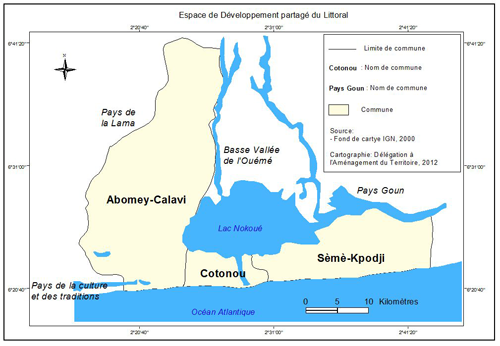
\includegraphics[width=.75\textwidth]{figures/littoral_carte}}
\end{figure}

\begin{singlespacing}

\providecommand{\docline}[3]{\noalign{\global\setlength{\arrayrulewidth}{#1}}\arrayrulecolor[HTML]{#2}\cline{#3}}

\setlength{\tabcolsep}{0pt}

\renewcommand*{\arraystretch}{1.5}

\begin{longtable}[c]{|p{1.00in}|p{0.80in}|p{0.80in}|p{0.80in}}

\caption{\textcolor[HTML]{000000}{\fontsize{11}{13}\selectfont{\global\setmainfont{Palatino}{Census\ of\ 13\ zones\ de\ dénombrement}}}}\label{tab:tbl-census}\\

\hhline{~~~~}

\multicolumn{1}{!{\color[HTML]{FFFFFF}\vrule width 0pt}>{\centering}p{\dimexpr 1in+0\tabcolsep+0\arrayrulewidth}}{\textcolor[HTML]{000000}{\fontsize{9}{18}\selectfont{\global\setmainfont{Times New Roman}{\ }}}} & \multicolumn{1}{!{\color[HTML]{FFFFFF}\vrule width 0pt}>{\centering}p{\dimexpr 0.8in+0\tabcolsep+0\arrayrulewidth}}{\textcolor[HTML]{000000}{\fontsize{9}{18}\selectfont{\global\setmainfont{Times New Roman}{Aged\ 15-19}}}} & \multicolumn{1}{!{\color[HTML]{FFFFFF}\vrule width 0pt}>{\centering}p{\dimexpr 0.8in+0\tabcolsep+0\arrayrulewidth}}{\textcolor[HTML]{000000}{\fontsize{9}{18}\selectfont{\global\setmainfont{Times New Roman}{Aged\ 20-29}}}} & \multicolumn{1}{!{\color[HTML]{FFFFFF}\vrule width 0pt}>{\centering}p{\dimexpr 0.8in+0\tabcolsep+0\arrayrulewidth}!{\color[HTML]{FFFFFF}\vrule width 0pt}}{\textcolor[HTML]{000000}{\fontsize{9}{18}\selectfont{\global\setmainfont{Times New Roman}{Aged\ 30\ and\ above}}}} \\

\hhline{>{\arrayrulecolor[HTML]{000000}\global\arrayrulewidth=1pt}->{\arrayrulecolor[HTML]{000000}\global\arrayrulewidth=1pt}->{\arrayrulecolor[HTML]{000000}\global\arrayrulewidth=1pt}->{\arrayrulecolor[HTML]{000000}\global\arrayrulewidth=1pt}-}\endhead



\multicolumn{4}{!{\color[HTML]{FFFFFF}\vrule width 0pt}>{\raggedright}p{\dimexpr 3.4in+6\tabcolsep+3\arrayrulewidth}!{\color[HTML]{FFFFFF}\vrule width 0pt}}{\textcolor[HTML]{000000}{\fontsize{9}{9}\selectfont{\global\setmainfont{Palatino}{\textit{Notes:\ }}}}\textcolor[HTML]{000000}{\fontsize{9}{9}\selectfont{\global\setmainfont{Palatino}{n,\ \%.}}}} \\

\endfoot



\multicolumn{1}{!{\color[HTML]{FFFFFF}\vrule width 0pt}>{\centering}p{\dimexpr 1in+0\tabcolsep+0\arrayrulewidth}}{\textcolor[HTML]{000000}{\fontsize{9}{18}\selectfont{\global\setmainfont{Times New Roman}{In\ School}}}} & \multicolumn{1}{!{\color[HTML]{FFFFFF}\vrule width 0pt}>{\centering}p{\dimexpr 0.8in+0\tabcolsep+0\arrayrulewidth}}{\textcolor[HTML]{000000}{\fontsize{9}{18}\selectfont{\global\setmainfont{Times New Roman}{1417\ (71.64)}}}} & \multicolumn{1}{!{\color[HTML]{FFFFFF}\vrule width 0pt}>{\centering}p{\dimexpr 0.8in+0\tabcolsep+0\arrayrulewidth}}{\textcolor[HTML]{000000}{\fontsize{9}{18}\selectfont{\global\setmainfont{Times New Roman}{1144\ (31.07)}}}} & \multicolumn{1}{!{\color[HTML]{FFFFFF}\vrule width 0pt}>{\centering}p{\dimexpr 0.8in+0\tabcolsep+0\arrayrulewidth}!{\color[HTML]{FFFFFF}\vrule width 0pt}}{\textcolor[HTML]{000000}{\fontsize{9}{18}\selectfont{\global\setmainfont{Times New Roman}{87\ (1.35)}}}} \\





\multicolumn{1}{!{\color[HTML]{FFFFFF}\vrule width 0pt}>{\centering}p{\dimexpr 1in+0\tabcolsep+0\arrayrulewidth}}{\textcolor[HTML]{000000}{\fontsize{9}{18}\selectfont{\global\setmainfont{Times New Roman}{Other}}}} & \multicolumn{1}{!{\color[HTML]{FFFFFF}\vrule width 0pt}>{\centering}p{\dimexpr 0.8in+0\tabcolsep+0\arrayrulewidth}}{\textcolor[HTML]{000000}{\fontsize{9}{18}\selectfont{\global\setmainfont{Times New Roman}{125\ (6.32)}}}} & \multicolumn{1}{!{\color[HTML]{FFFFFF}\vrule width 0pt}>{\centering}p{\dimexpr 0.8in+0\tabcolsep+0\arrayrulewidth}}{\textcolor[HTML]{000000}{\fontsize{9}{18}\selectfont{\global\setmainfont{Times New Roman}{635\ (17.25)\ }}}} & \multicolumn{1}{!{\color[HTML]{FFFFFF}\vrule width 0pt}>{\centering}p{\dimexpr 0.8in+0\tabcolsep+0\arrayrulewidth}!{\color[HTML]{FFFFFF}\vrule width 0pt}}{\textcolor[HTML]{000000}{\fontsize{9}{18}\selectfont{\global\setmainfont{Times New Roman}{574\ (24.35)}}}} \\





\multicolumn{1}{!{\color[HTML]{FFFFFF}\vrule width 0pt}>{\centering}p{\dimexpr 1in+0\tabcolsep+0\arrayrulewidth}}{\textcolor[HTML]{000000}{\fontsize{9}{18}\selectfont{\global\setmainfont{Times New Roman}{Self-Employed}}}} & \multicolumn{1}{!{\color[HTML]{FFFFFF}\vrule width 0pt}>{\centering}p{\dimexpr 0.8in+0\tabcolsep+0\arrayrulewidth}}{\textcolor[HTML]{000000}{\fontsize{9}{18}\selectfont{\global\setmainfont{Times New Roman}{95\ (4.80)}}}} & \multicolumn{1}{!{\color[HTML]{FFFFFF}\vrule width 0pt}>{\centering}p{\dimexpr 0.8in+0\tabcolsep+0\arrayrulewidth}}{\textcolor[HTML]{000000}{\fontsize{9}{18}\selectfont{\global\setmainfont{Times New Roman}{1183\ (32.13)\ }}}} & \multicolumn{1}{!{\color[HTML]{FFFFFF}\vrule width 0pt}>{\centering}p{\dimexpr 0.8in+0\tabcolsep+0\arrayrulewidth}!{\color[HTML]{FFFFFF}\vrule width 0pt}}{\textcolor[HTML]{000000}{\fontsize{9}{18}\selectfont{\global\setmainfont{Times New Roman}{664\ (56.68)}}}} \\





\multicolumn{1}{!{\color[HTML]{FFFFFF}\vrule width 0pt}>{\centering}p{\dimexpr 1in+0\tabcolsep+0\arrayrulewidth}}{\textcolor[HTML]{000000}{\fontsize{9}{18}\selectfont{\global\setmainfont{Times New Roman}{Employed}}}} & \multicolumn{1}{!{\color[HTML]{FFFFFF}\vrule width 0pt}>{\centering}p{\dimexpr 0.8in+0\tabcolsep+0\arrayrulewidth}}{\textcolor[HTML]{000000}{\fontsize{9}{18}\selectfont{\global\setmainfont{Times New Roman}{35\ (1.77)}}}} & \multicolumn{1}{!{\color[HTML]{FFFFFF}\vrule width 0pt}>{\centering}p{\dimexpr 0.8in+0\tabcolsep+0\arrayrulewidth}}{\textcolor[HTML]{000000}{\fontsize{9}{18}\selectfont{\global\setmainfont{Times New Roman}{33\ (11.76)}}}} & \multicolumn{1}{!{\color[HTML]{FFFFFF}\vrule width 0pt}>{\centering}p{\dimexpr 0.8in+0\tabcolsep+0\arrayrulewidth}!{\color[HTML]{FFFFFF}\vrule width 0pt}}{\textcolor[HTML]{000000}{\fontsize{9}{18}\selectfont{\global\setmainfont{Times New Roman}{117\ (17.28)}}}} \\





\multicolumn{1}{!{\color[HTML]{FFFFFF}\vrule width 0pt}>{\centering}p{\dimexpr 1in+0\tabcolsep+0\arrayrulewidth}}{\textcolor[HTML]{000000}{\fontsize{9}{18}\selectfont{\global\setmainfont{Times New Roman}{Apprentice}}}} & \multicolumn{1}{!{\color[HTML]{FFFFFF}\vrule width 0pt}>{\centering}p{\dimexpr 0.8in+0\tabcolsep+0\arrayrulewidth}}{\textcolor[HTML]{000000}{\fontsize{9}{18}\selectfont{\global\setmainfont{Times New Roman}{306\ (15.47)}}}} & \multicolumn{1}{!{\color[HTML]{FFFFFF}\vrule width 0pt}>{\centering}p{\dimexpr 0.8in+0\tabcolsep+0\arrayrulewidth}}{\textcolor[HTML]{000000}{\fontsize{9}{18}\selectfont{\global\setmainfont{Times New Roman}{\ 287\ (7.79)}}}} & \multicolumn{1}{!{\color[HTML]{FFFFFF}\vrule width 0pt}>{\centering}p{\dimexpr 0.8in+0\tabcolsep+0\arrayrulewidth}!{\color[HTML]{FFFFFF}\vrule width 0pt}}{\textcolor[HTML]{000000}{\fontsize{9}{18}\selectfont{\global\setmainfont{Times New Roman}{22\ (0.34)}}}} \\





\multicolumn{1}{!{\color[HTML]{FFFFFF}\vrule width 0pt}>{\centering}p{\dimexpr 1in+0\tabcolsep+0\arrayrulewidth}}{\textcolor[HTML]{000000}{\fontsize{9}{18}\selectfont{\global\setmainfont{Times New Roman}{Total}}}} & \multicolumn{1}{!{\color[HTML]{FFFFFF}\vrule width 0pt}>{\centering}p{\dimexpr 0.8in+0\tabcolsep+0\arrayrulewidth}}{\textcolor[HTML]{000000}{\fontsize{9}{18}\selectfont{\global\setmainfont{Times New Roman}{1978\ (100.00)}}}} & \multicolumn{1}{!{\color[HTML]{FFFFFF}\vrule width 0pt}>{\centering}p{\dimexpr 0.8in+0\tabcolsep+0\arrayrulewidth}}{\textcolor[HTML]{000000}{\fontsize{9}{18}\selectfont{\global\setmainfont{Times New Roman}{3682\ (100.00)}}}} & \multicolumn{1}{!{\color[HTML]{FFFFFF}\vrule width 0pt}>{\centering}p{\dimexpr 0.8in+0\tabcolsep+0\arrayrulewidth}!{\color[HTML]{FFFFFF}\vrule width 0pt}}{\textcolor[HTML]{000000}{\fontsize{9}{18}\selectfont{\global\setmainfont{Times New Roman}{6464\ (100.00)}}}} \\

\hhline{>{\arrayrulecolor[HTML]{000000}\global\arrayrulewidth=1pt}->{\arrayrulecolor[HTML]{000000}\global\arrayrulewidth=1pt}->{\arrayrulecolor[HTML]{000000}\global\arrayrulewidth=1pt}->{\arrayrulecolor[HTML]{000000}\global\arrayrulewidth=1pt}-}



\end{longtable}
\end{singlespacing}

\newpage

\hypertarget{sampling}{%
\subsection*{Sampling}\label{sampling}}

\markboth{Sampling}{Appendix A3}

Cluster sampling was used to select the 752 youth interviewed in the face-to-face baseline survey. The twelve \emph{départements} of Bénin are subdivided into 77 \emph{communes}, which are further subdivided into \emph{arrondissements}. To delimit the geographic area for the census, we first manually selected five \emph{arrondissements} from the three \emph{communes} which constitute the Cotonou metropolitan area (Figure \ref{fig:litt}). The five \emph{arrondissements} were chosen in consultation with survey partners experienced in data collection in the region to be as representative of urban Cotonou as possible.

In a second step, 15 Zones de dénombrement (ZDs) -- the smallest administrative divisions in Bénin -- were selected from the five \emph{arrondissements} (or clusters) and constitute the primary sampling unit (PSU) of the sample. The number of ZDs chosen per cluster was proportional to the size of the youth population in each \emph{arrondissement} at the time of the 2016 census, such that each household in the five \emph{arrondissements} still had an equally likely chance of being sampled and no reweighting was necessary. Eight ZDs were thus drawn from the \emph{arrondissement} of Cotonou, two from Godomey, two from Calavi, one from Agbanglandan, and one from Ekpè.

All 4,905 households living in within the boundaries of these 15 ZDs were interviewed in person to ascertain the age and employment status (in school, in apprenticeship, employed, self-employed, or inactive) of all household members. Table \ref{tab:tbl-census} in Appendix A3 shows that a total of 19,032 individuals were covered by the census, with all individuals aged 20-29 in these households (excluding apprentices, due to overlap with a second study by the author\footnote{A number of apprentices appear in the final sample due to misreporting or a change in activity between the time of the census and the baseline interview.}) constituting the sample frame for the panel survey. Survey participants were selected randomly from this pool of 3,395 youth; the survey is thus representative of youth aged 20-29 in the metropolitan area of Cotonou whose primary economic activity is not apprenticeship training.

\markboth{Appendix A3}{Appendix A3}
\newpage
\begin{table}[H]

\caption{\label{tab:tbl-attrition}Sample Composition and Attrition}
\centering
\begin{threeparttable}
\fontsize{8}{10}\selectfont
\begin{tabular}[t]{l>{\centering\arraybackslash}p{6em}>{\centering\arraybackslash}p{6em}>{\centering\arraybackslash}p{6em}>{\centering\arraybackslash}p{6em}>{\centering\arraybackslash}p{6em}>{\centering\arraybackslash}p{4em}}
\toprule
\textbf{Characteristic} & \textbf{Baseline}\newline N=752 & \textbf{Follow-up 1}\newline N=663 & \textbf{Follow-up 2}\newline N=536 & \textbf{Follow-up 3}\newline N=496 & \textbf{Endline}\newline N=574 & \textbf{p-value}\\
\midrule
Activity &  &  &  &  &  & <0.001\\
\hspace{1em}Apprentice & 58 (7.7\%) & 40 (6.0\%) & 39 (7.3\%) & 24 (4.8\%) & 21 (3.7\%) & \\
\hspace{1em}In School & 169 (22\%) & 124 (19\%) & 95 (18\%) & 74 (15\%) & 60 (10\%) & \\
\hspace{1em}Employed & 168 (22\%) & 176 (27\%) & 164 (31\%) & 165 (33\%) & 185 (32\%) & \\
\hspace{1em}Self-Employed & 119 (16\%) & 148 (22\%) & 106 (20\%) & 93 (19\%) & 135 (24\%) & \\
\hspace{1em}NEET & 238 (32\%) & 175 (26\%) & 132 (25\%) & 140 (28\%) & 173 (30\%) & \\
Baseline activity &  &  &  &  &  & 0.31\\
\hspace{1em}Apprentice & 58 (7.7\%) & 49 (7.4\%) & 45 (8.4\%) & 48 (9.7\%) & 51 (8.9\%) & \\
\hspace{1em}In School & 169 (22\%) & 151 (23\%) & 132 (25\%) & 124 (25\%) & 144 (25\%) & \\
\hspace{1em}Employed & 168 (22\%) & 153 (23\%) & 122 (23\%) & 107 (22\%) & 124 (22\%) & \\
\hspace{1em}Self-Employed & 119 (16\%) & 105 (16\%) & 74 (14\%) & 73 (15\%) & 94 (16\%) & \\
\hspace{1em}NEET & 238 (32\%) & 205 (31\%) & 163 (30\%) & 144 (29\%) & 161 (28\%) & \\
Male & 47\% & 48\% & 52\% & 52\% & 52\% & 0.26\\
Age & 24.15 (2.67) & 24.19 (2.67) & 23.99 (2.65) & 24.05 (2.67) & 24.09 (2.67) & 0.76\\
Years of Schooling & 13.5 (4.7) & 13.6 (4.6) & 13.9 (4.5) & 13.8 (4.5) & 13.7 (4.4) & 0.40\\
\bottomrule
\end{tabular}
\begin{tablenotes}
\item \textit{Notes:} n (\%); \%; Mean (SD). Calculated using responses from baseline survey. 
\end{tablenotes}
\end{threeparttable}
\end{table}
\newpage

\hypertarget{markovapp}{%
\subsection*{Transitions as Markov processes}\label{markovapp}}

\markboth{Studying transitions as continuous Markov processes}{Appendix A3}

In Appendix B, we depict transitions between \(K\) states employment states as transition intensity matrices. Each cell of the transition intensity matrix is given by the probability of transitioning from an initial employment state \(i\) to a subsequent employment state \(j\), which is simply given by \(p_{ij} = n_{ij}/n_i\), such that the matrices in Appendix B can be depicted as

\begin{singlespacing}
$$
Q= \begin{pmatrix}
p_{11} & \dots & p_{1k}\\
\vdots & \ddots & \vdots \\
p_{k1} &\dots & p_{kk} \\
\end{pmatrix}
$$
\end{singlespacing}

where \(n_{ij}\) is the number of youth making the transition from state \(i\) to \(j\) and \(n_i\) is the number of youth in the initial state \(i\).

Transition intensity matrices alone do not allow us to make informative comparisons between subgroups, as we do not know if a higher \(p_{ij}\) indicates a preference of a subgroup for a certain transition, or simply higher turnover. To mitigate this issue, we follow \textcite{bosch2007} and \textcite{cunningham2011} in decomposing the transition intensity matrices into two separate elements, which allow us to infer the propensity at which groups make certain transitions independent of that group's likelihood to change states.

``Since we have access to discrete panel data, rather than continuous time data, equation (1) can be interpreted as the transition probability if we assume that the discrete-time mobility process captured by our data is generated by a continuous-time homogenous Markov process. In other words, if we assume that transitions between states occur at random points in time, then a random draw of a transition in one point in time has the same probability (within a confidence interval) of a draw at any other point in time.''

This rate of transition, which can be referred to as intensities \autocite{bosch2007}, make differences across different groups (age groups or gender) difficult because they do not account for the likelihood of separation (i.e.~changing states). For example, younger individuals are much less likely to transition out of school; thus, the rate of transition from school to, say, wage employment will be deflated relative to older youth around school-leaving age, and will tell us little about the preference of younger school-leavers for wage employment relative to other options.

The method proposed by \textcite{bosch2007} and \textcite{bosch2010} and applied to youth transitions by \textcite{cunningham2011} controls for the likelihood of separation by
factoring \(Q\) into two elements, the rate of separation and the propensity to move, denoted by \(Q = \lambda(M-I)\):

\begin{singlespacing}
$$
Q= \begin{pmatrix}
-p_{11} &  &  &  \\
 & \ddots &  &  \\
 &   & -p_{kk} & \\
\end{pmatrix}
\begin{pmatrix} \begin{bmatrix}
0 &  r_{ij} & \\
 & \ddots &  \\
 &  & 0  \\
\end{bmatrix} - I
\end{pmatrix}
$$
\end{singlespacing}

where \(r_{ij} = -p_{ij}/p_{ii}\) for \(i \neq j\) and \(i = 1, \dots, K\) and \(I\) is the identity matrix.

The first component represents the transition probabilities independent of the rate at which different age groups leave any sector, and is called the propensity matrix. The second is the rate of transition, and is referred to as the rate of separation matrix. By decomposing the transition intensity matrix into the propensity matrix and the rate of separation matrix, we can determine if movements to employment states observed in the transition intensity matrix are reflecting greater entry of certain age groups into certain employment states or if the observed transitions are simply due to greater turnover by certain age groups in general.

\markboth{Appendix A3}{Appendix A3}

\begin{singlespacing}
\renewcommand{\arraystretch}{1.2}

\begin{table}[H]

\caption{\label{tab:tbl-descgender}Summary Statistics By Gender}
\centering
\begin{threeparttable}
\fontsize{8}{10}\selectfont
\begin{tabular}[t]{l>{\centering\arraybackslash}p{7em}>{\centering\arraybackslash}p{7em}>{\centering\arraybackslash}p{7em}>{\centering\arraybackslash}p{7em}}
\toprule
\multicolumn{2}{c}{ } & \multicolumn{2}{c}{\textbf{Gender}} & \multicolumn{1}{c}{ } \\
\cmidrule(l{3pt}r{3pt}){3-4}
\textbf{Characteristic} & \textbf{Overall} & \textbf{Female} (53\%) & \textbf{Male} (47\%) & \textbf{p-value}\\
\midrule
N & 752 & 396 & 356 & \\
Age at baseline & 24.15 (24.00) & 24.03 (24.00) & 24.29 (24.00) & 0.13\\
Nationality: Beninese (=1) & 97\% & 96\% & 99\% & 0.043\\
Ethnicity: Fon (=1) & 69\% & 69\% & 69\% & >0.9\\
Religion: Christian (=1) & 84\% & 89\% & 78\% & <0.001\\
Grew up in a city (=1) & 64\% & 65\% & 63\% & 0.6\\
\addlinespace[0.3em]
\multicolumn{5}{l}{\textbf{School-to-Work Transition}}\\
\hspace{1em}School-leaving age & 22.62 (23.00) & 22.27 (22.00) & 22.90 (23.00) & 0.004\\
\hspace{1em}Had first work experience & 60\% & 51\% & 70\% & <0.001\\
\hspace{1em}Age at first work experience & 23.37 (23.00) & 23.08 (23.00) & 23.60 (24.00) & 0.023\\
\hspace{1em}Status at first work exp. &  &  &  & 0.7\\
\hspace{1em}\hspace{1em}Employed & 63\% & 62\% & 63\% & \\
\hspace{1em}\hspace{1em}Self-Employed & 37\% & 38\% & 37\% & \\
\hspace{1em}Completed SWT & 55\% & 47\% & 65\% & <0.001\\
\hspace{1em}Age at labor market entry & 23.65 (24.00) & 23.36 (23.00) & 23.88 (24.00) & 0.025\\
\hspace{1em}Status at labour market entry &  &  &  & 0.2\\
\hspace{1em}\hspace{1em}Employed & 63\% & 59\% & 65\% & \\
\hspace{1em}\hspace{1em}Self-Employed & 37\% & 41\% & 35\% & \\
\hspace{1em}Duration of transition in years¹ & 1.06 (1.00) & 1.13 (1.00) & 1.01 (1.00) & 0.2\\
\addlinespace[0.3em]
\multicolumn{5}{l}{\textbf{Education}}\\
\hspace{1em}Years of schooling & 13 (15) & 13 (14) & 14 (15) & <0.001\\
\hspace{1em}Completed apprenticeship (=1) & 20\% & 20\% & 20\% & 0.8\\
\hspace{1em}Vocational certificate: CAP (=1) & 4.4\% & 4.0\% & 4.8\% & 0.6\\
\hspace{1em}Primary diploma: CEP (=1) & 85\% & 80\% & 90\% & <0.001\\
\hspace{1em}Junior high diploma: BEPC (=1) & 67\% & 61\% & 74\% & <0.001\\
\hspace{1em}Baccalauréat: BAC (=1) & 40\% & 32\% & 48\% & <0.001\\
\hspace{1em}2nd cycle university: Licence (=1) & 15\% & 11\% & 20\% & 0.002\\
\hspace{1em}3rd cycle university: Maîtrise (=1) & 2.3\% & 0.5\% & 4.2\% & <0.001\\
\addlinespace[0.3em]
\multicolumn{5}{l}{\textbf{Parents' Education}}\\
\hspace{1em}Father was an apprentice (=1) & 33\% & 32\% & 33\% & 0.9\\
\hspace{1em}Father completed primary (=1) & 67\% & 67\% & 67\% & 0.9\\
\hspace{1em}Father completed secondary (=1) & 41\% & 43\% & 38\% & 0.11\\
\hspace{1em}Mother was an apprentice (=1) & 17\% & 18\% & 16\% & 0.5\\
\hspace{1em}Mother completed primary (=1) & 41\% & 41\% & 41\% & >0.9\\
\hspace{1em}Mother completed secondary (=1) & 20\% & 19\% & 20\% & 0.9\\
\addlinespace[0.3em]
\multicolumn{5}{l}{\textbf{Household Characteristics and Assets}}\\
\hspace{1em}Married (=1) & 20\% & 28\% & 10\% & <0.001\\
\hspace{1em}Living with parents (=1) & 45\% & 42\% & 49\% & 0.057\\
\hspace{1em}No. of children & 1.61 (1.00) & 1.87 (1.00) & 1.32 (1.00) & <0.001\\
\hspace{1em}People in household & 6.45 (6.00) & 6.67 (6.00) & 6.20 (6.00) & 0.034\\
\hspace{1em}Wealth index quintile & 2.91 (3.00) & 2.86 (3.00) & 2.96 (3.00) & 0.3\\
\hspace{1em}Home electrified (=1) & 92\% & 93\% & 92\% & 0.5\\
\hspace{1em}Cell Phone (=1) & 76\% & 75\% & 76\% & 0.7\\
\hspace{1em}Smartphone (=1) & 54\% & 47\% & 62\% & <0.001\\
\hspace{1em}Motorcycle (=1) & 27\% & 18\% & 38\% & <0.001\\
\hspace{1em}Television (=1) & 39\% & 39\% & 40\% & 0.9\\
\bottomrule
\end{tabular}
\begin{tablenotes}
\item \scriptsize{\textit{Notes:} Mean (median); \%. Calculated using responses from baseline survey.}
\item[1] To labor market entry, defined as first work experience with no subsequent return to schooling or training.
\end{tablenotes}
\end{threeparttable}
\end{table}

\newpage

\begin{table}[H]

\caption{\label{tab:tbl-entry-full}Labour Market Entry - Detailed Summary Statistics}
\centering
\begin{threeparttable}
\fontsize{9}{11}\selectfont
\begin{tabular}[t]{l>{\centering\arraybackslash}p{5em}>{\centering\arraybackslash}p{5em}>{\centering\arraybackslash}p{5em}>{\centering\arraybackslash}p{5em}>{\centering\arraybackslash}p{5em}}
\toprule
\multicolumn{2}{c}{ } & \multicolumn{3}{c}{\makecell[c]{\textit{}Status in first \\period after school-leaving\textit{}}} & \multicolumn{1}{c}{ } \\
\cmidrule(l{3pt}r{3pt}){3-5}
\textbf{Characteristic} & \textbf{Overall} & \textbf{Employed} (38\%) & \textbf{NEET} (37\%) & \textbf{Self-}\newline \textbf{Employed} (24\%) & \textbf{p-value}\\
\midrule
N & 471 & 181 & 176 & 114 & \\
Male & 55\% & 61\% & 48\% & 54\% & 0.047\\
\addlinespace[0.3em]
\multicolumn{6}{l}{\textbf{School-to-Work Transition}}\\
\hspace{1em}School-leaving age & 22.62 & 22.66 & 22.76 & 22.33 & 0.3\\
\hspace{1em}Had first work experience (=1) & 91\% & 100\% & 75\% & 100\% & <0.001\\
\hspace{1em}Age at first work experience & 23.38 & 23.19 & 24.05 & 22.90 & 0.002\\
\hspace{1em}First work experience &  &  &  &  & <0.001\\
\hspace{1em}\hspace{1em}Employed & 62\% & 95\% & 66\% & 4.4\% & \\
\hspace{1em}\hspace{1em}Self-Employed & 38\% & 5.0\% & 34\% & 96\% & \\
\hspace{1em}Completed SWT (=1) & 89\% & 100\% & 69\% & 100\% & <0.001\\
\hspace{1em}Age at labor market entry & 23.65 & 23.47 & 24.42 & 23.11 & <0.001\\
\hspace{1em}Status at labor market entry &  &  &  &  & <0.001\\
\hspace{1em}\hspace{1em}Employed & 63\% & 100\% & 66\% & 0\% & \\
\hspace{1em}\hspace{1em}Self-Employed & 37\% & 0\% & 34\% & 100\% & \\
\hspace{1em}Duration of transition in years¹ & 1.06 & 0.81 & 1.70 & 0.78 & <0.001\\
\addlinespace[0.3em]
\multicolumn{6}{l}{\textbf{Education}}\\
\hspace{1em}Years of schooling & 14.3 & 14.8 & 14.5 & 13.4 & 0.032\\
\hspace{1em}Completed apprenticeship (=1) & 20\% & 19\% & 14\% & 28\% & 0.014\\
\hspace{1em}Vocational certificate: CAP (=1) & 5.1\% & 5.5\% & 4.0\% & 6.1\% & 0.7\\
\hspace{1em}Primary diploma: CEP (=1) & 91\% & 93\% & 91\% & 87\% & 0.2\\
\hspace{1em}Junior high diploma: BEPC (=1) & 74\% & 77\% & 78\% & 63\% & 0.009\\
\hspace{1em}Baccalauréat: BAC (=1) & 46\% & 51\% & 47\% & 38\% & 0.071\\
\hspace{1em}2nd cycle university: Licence (=1) & 20\% & 20\% & 24\% & 16\% & 0.2\\
\hspace{1em}3rd cycle university: Maîtrise (=1) & 3.4\% & 3.3\% & 4.0\% & 2.6\% & 0.9\\
\addlinespace[0.3em]
\multicolumn{6}{l}{\textbf{Parents' Education}}\\
\hspace{1em}\hspace{1em}Father was an apprentice (=1) & 34\% & 35\% & 32\% & 34\% & 0.9\\
\hspace{1em}Father completed primary (=1) & 69\% & 71\% & 70\% & 65\% & 0.5\\
\hspace{1em}Father completed secondary (=1) & 42\% & 43\% & 46\% & 36\% & 0.2\\
\hspace{1em}Mother was an apprentice (=1) & 17\% & 15\% & 19\% & 18\% & 0.6\\
\hspace{1em}Mother completed primary (=1) & 45\% & 46\% & 47\% & 39\% & 0.3\\
\hspace{1em}Mother completed secondary (=1) & 21\% & 20\% & 23\% & 20\% & 0.8\\
\hspace{1em}Married (=1) & 13\% & 10\% & 15\% & 15\% & 0.4\\
\addlinespace[0.3em]
\multicolumn{6}{l}{\textbf{Household Characteristics and Assets}}\\
\hspace{1em}Living with parents (=1) & 47\% & 47\% & 47\% & 49\% & >0.9\\
\hspace{1em}No. of children & 1.42 & 1.36 & 1.42 & 1.50 & 0.4\\
\hspace{1em}People in household & 6.23 & 6.36 & 6.26 & 6.00 & 0.7\\
\hspace{1em}Wealth index quintile & 2.98 & 2.94 & 2.97 & 3.04 & 0.8\\
\bottomrule
\end{tabular}
\begin{tablenotes}
\item \textit{Notes:} Mean; \%. Calculated using responses from baseline survey.
\item[1] To labor market entry, defined as first work experience with no subsequent return to school or training.
\end{tablenotes}
\end{threeparttable}
\end{table}

\newpage


\providecommand{\docline}[3]{\noalign{\global\setlength{\arrayrulewidth}{#1}}\arrayrulecolor[HTML]{#2}\cline{#3}}

\setlength{\tabcolsep}{0pt}

\renewcommand*{\arraystretch}{1}

\begin{longtable}[c]{|p{0.70in}|p{0.70in}|p{0.70in}|p{0.70in}|p{0.70in}|p{0.70in}|p{0.70in}|p{0.40in}}

\caption{\textcolor[HTML]{000000}{\fontsize{11}{13}\selectfont{\global\setmainfont{Palatino}{Transition\ Rates\ into\ Various\ Types\ of\ Work}}}}\label{tab:tbl-propensities}\\

\hhline{~~~~~~~~}

\multicolumn{4}{!{\color[HTML]{FFFFFF}\vrule width 0pt}>{\centering}p{\dimexpr 2.8in+6\tabcolsep+3\arrayrulewidth}}{\textcolor[HTML]{000000}{\fontsize{9}{18}\selectfont{\global\setmainfont{Times New Roman}{}}}} & \multicolumn{4}{!{\color[HTML]{FFFFFF}\vrule width 0pt}>{\centering}p{\dimexpr 2.5in+6\tabcolsep+3\arrayrulewidth}!{\color[HTML]{FFFFFF}\vrule width 0pt}}{\textcolor[HTML]{000000}{\fontsize{9}{18}\selectfont{\global\setmainfont{Times New Roman}{To}}}} \\

\hhline{>{\arrayrulecolor[HTML]{000000}\global\arrayrulewidth=1pt}->{\arrayrulecolor[HTML]{000000}\global\arrayrulewidth=1pt}->{\arrayrulecolor[HTML]{000000}\global\arrayrulewidth=1pt}->{\arrayrulecolor[HTML]{000000}\global\arrayrulewidth=1pt}->{\arrayrulecolor[HTML]{000000}\global\arrayrulewidth=1pt}->{\arrayrulecolor[HTML]{000000}\global\arrayrulewidth=1pt}->{\arrayrulecolor[HTML]{000000}\global\arrayrulewidth=1pt}->{\arrayrulecolor[HTML]{000000}\global\arrayrulewidth=1pt}-}



\multicolumn{1}{!{\color[HTML]{FFFFFF}\vrule width 0pt}>{\centering}p{\dimexpr 0.7in+0\tabcolsep+0\arrayrulewidth}}{\textcolor[HTML]{000000}{\fontsize{9}{18}\selectfont{\global\setmainfont{Times New Roman}{From}}}} & \multicolumn{1}{!{\color[HTML]{FFFFFF}\vrule width 0pt}>{\centering}p{\dimexpr 0.7in+0\tabcolsep+0\arrayrulewidth}}{\textcolor[HTML]{000000}{\fontsize{9}{18}\selectfont{\global\setmainfont{Times New Roman}{Formal}}}} & \multicolumn{1}{!{\color[HTML]{FFFFFF}\vrule width 0pt}>{\centering}p{\dimexpr 0.7in+0\tabcolsep+0\arrayrulewidth}}{\textcolor[HTML]{000000}{\fontsize{9}{18}\selectfont{\global\setmainfont{Times New Roman}{Informal}}}} & \multicolumn{1}{!{\color[HTML]{FFFFFF}\vrule width 0pt}>{\centering}p{\dimexpr 0.7in+0\tabcolsep+0\arrayrulewidth}}{\textcolor[HTML]{000000}{\fontsize{9}{18}\selectfont{\global\setmainfont{Times New Roman}{Regular}}}} & \multicolumn{1}{!{\color[HTML]{FFFFFF}\vrule width 0pt}>{\centering}p{\dimexpr 0.7in+0\tabcolsep+0\arrayrulewidth}}{\textcolor[HTML]{000000}{\fontsize{9}{18}\selectfont{\global\setmainfont{Times New Roman}{Casual}}}} & \multicolumn{1}{!{\color[HTML]{FFFFFF}\vrule width 0pt}>{\centering}p{\dimexpr 0.7in+0\tabcolsep+0\arrayrulewidth}}{\textcolor[HTML]{000000}{\fontsize{9}{18}\selectfont{\global\setmainfont{Times New Roman}{Under-}}}\textcolor[HTML]{000000}{\fontsize{9}{18}\selectfont{\global\setmainfont{Times New Roman}{\linebreak }}}\textcolor[HTML]{000000}{\fontsize{9}{18}\selectfont{\global\setmainfont{Times New Roman}{employed}}}} & \multicolumn{1}{!{\color[HTML]{FFFFFF}\vrule width 0pt}>{\centering}p{\dimexpr 0.7in+0\tabcolsep+0\arrayrulewidth}}{\textcolor[HTML]{000000}{\fontsize{9}{18}\selectfont{\global\setmainfont{Times New Roman}{Employer}}}} & \multicolumn{1}{!{\color[HTML]{FFFFFF}\vrule width 0pt}>{\centering}p{\dimexpr 0.4in+0\tabcolsep+0\arrayrulewidth}!{\color[HTML]{FFFFFF}\vrule width 0pt}}{\textcolor[HTML]{000000}{\fontsize{9}{18}\selectfont{\global\setmainfont{Times New Roman}{Indep.}}}} \\

\hhline{>{\arrayrulecolor[HTML]{000000}\global\arrayrulewidth=1pt}->{\arrayrulecolor[HTML]{000000}\global\arrayrulewidth=1pt}->{\arrayrulecolor[HTML]{000000}\global\arrayrulewidth=1pt}->{\arrayrulecolor[HTML]{000000}\global\arrayrulewidth=1pt}->{\arrayrulecolor[HTML]{000000}\global\arrayrulewidth=1pt}->{\arrayrulecolor[HTML]{000000}\global\arrayrulewidth=1pt}->{\arrayrulecolor[HTML]{000000}\global\arrayrulewidth=1pt}->{\arrayrulecolor[HTML]{000000}\global\arrayrulewidth=1pt}-}\endhead



\multicolumn{8}{!{\color[HTML]{FFFFFF}\vrule width 0pt}>{\raggedright}p{\dimexpr 5.3in+14\tabcolsep+7\arrayrulewidth}!{\color[HTML]{FFFFFF}\vrule width 0pt}}{\textcolor[HTML]{000000}{\fontsize{9}{9}\selectfont{\global\setmainfont{Palatino}{\textit{Notes:\ }}}}\textcolor[HTML]{000000}{\fontsize{9}{9}\selectfont{\global\setmainfont{Palatino}{Row\ \%s\ reported,\ but\ do\ not\ add\ up\ to\ 100\%\ as\ activities\ are\ not\ exclusive.}}}} \\

\endfoot



\multicolumn{1}{!{\color[HTML]{FFFFFF}\vrule width 0pt}>{\centering}p{\dimexpr 0.7in+0\tabcolsep+0\arrayrulewidth}}{\textcolor[HTML]{000000}{\fontsize{9}{18}\selectfont{\global\setmainfont{Times New Roman}{\textbf{In\ School}}}}} & \multicolumn{1}{!{\color[HTML]{FFFFFF}\vrule width 0pt}>{\centering}p{\dimexpr 0.7in+0\tabcolsep+0\arrayrulewidth}}{\textcolor[HTML]{000000}{\fontsize{9}{18}\selectfont{\global\setmainfont{Times New Roman}{\textbf{8.77\%}}}}} & \multicolumn{1}{!{\color[HTML]{FFFFFF}\vrule width 0pt}>{\centering}p{\dimexpr 0.7in+0\tabcolsep+0\arrayrulewidth}}{\textcolor[HTML]{000000}{\fontsize{9}{18}\selectfont{\global\setmainfont{Times New Roman}{\textbf{7.88\%}}}}} & \multicolumn{1}{!{\color[HTML]{FFFFFF}\vrule width 0pt}>{\centering}p{\dimexpr 0.7in+0\tabcolsep+0\arrayrulewidth}}{\textcolor[HTML]{000000}{\fontsize{9}{18}\selectfont{\global\setmainfont{Times New Roman}{\textbf{5.19\%}}}}} & \multicolumn{1}{!{\color[HTML]{FFFFFF}\vrule width 0pt}>{\centering}p{\dimexpr 0.7in+0\tabcolsep+0\arrayrulewidth}}{\textcolor[HTML]{000000}{\fontsize{9}{18}\selectfont{\global\setmainfont{Times New Roman}{\textbf{10.03\%}}}}} & \multicolumn{1}{!{\color[HTML]{FFFFFF}\vrule width 0pt}>{\centering}p{\dimexpr 0.7in+0\tabcolsep+0\arrayrulewidth}}{\textcolor[HTML]{000000}{\fontsize{9}{18}\selectfont{\global\setmainfont{Times New Roman}{\textbf{8.89\%}}}}} & \multicolumn{1}{!{\color[HTML]{FFFFFF}\vrule width 0pt}>{\centering}p{\dimexpr 0.7in+0\tabcolsep+0\arrayrulewidth}}{\textcolor[HTML]{000000}{\fontsize{9}{18}\selectfont{\global\setmainfont{Times New Roman}{\textbf{7.04\%}}}}} & \multicolumn{1}{!{\color[HTML]{FFFFFF}\vrule width 0pt}>{\centering}p{\dimexpr 0.4in+0\tabcolsep+0\arrayrulewidth}!{\color[HTML]{FFFFFF}\vrule width 0pt}}{\textcolor[HTML]{000000}{\fontsize{9}{18}\selectfont{\global\setmainfont{Times New Roman}{\textbf{5.24\%}}}}} \\





\multicolumn{1}{!{\color[HTML]{FFFFFF}\vrule width 0pt}>{\centering}p{\dimexpr 0.7in+0\tabcolsep+0\arrayrulewidth}}{\textcolor[HTML]{000000}{\fontsize{9}{18}\selectfont{\global\setmainfont{Times New Roman}{\ \ \ \ Female}}}} & \multicolumn{1}{!{\color[HTML]{FFFFFF}\vrule width 0pt}>{\centering}p{\dimexpr 0.7in+0\tabcolsep+0\arrayrulewidth}}{\textcolor[HTML]{000000}{\fontsize{9}{18}\selectfont{\global\setmainfont{Times New Roman}{6.25\%}}}} & \multicolumn{1}{!{\color[HTML]{FFFFFF}\vrule width 0pt}>{\centering}p{\dimexpr 0.7in+0\tabcolsep+0\arrayrulewidth}}{\textcolor[HTML]{000000}{\fontsize{9}{18}\selectfont{\global\setmainfont{Times New Roman}{6.86\%}}}} & \multicolumn{1}{!{\color[HTML]{FFFFFF}\vrule width 0pt}>{\centering}p{\dimexpr 0.7in+0\tabcolsep+0\arrayrulewidth}}{\textcolor[HTML]{000000}{\fontsize{9}{18}\selectfont{\global\setmainfont{Times New Roman}{5.56\%}}}} & \multicolumn{1}{!{\color[HTML]{FFFFFF}\vrule width 0pt}>{\centering}p{\dimexpr 0.7in+0\tabcolsep+0\arrayrulewidth}}{\textcolor[HTML]{000000}{\fontsize{9}{18}\selectfont{\global\setmainfont{Times New Roman}{8.87\%}}}} & \multicolumn{1}{!{\color[HTML]{FFFFFF}\vrule width 0pt}>{\centering}p{\dimexpr 0.7in+0\tabcolsep+0\arrayrulewidth}}{\textcolor[HTML]{000000}{\fontsize{9}{18}\selectfont{\global\setmainfont{Times New Roman}{7.28\%}}}} & \multicolumn{1}{!{\color[HTML]{FFFFFF}\vrule width 0pt}>{\centering}p{\dimexpr 0.7in+0\tabcolsep+0\arrayrulewidth}}{\textcolor[HTML]{000000}{\fontsize{9}{18}\selectfont{\global\setmainfont{Times New Roman}{6.12\%}}}} & \multicolumn{1}{!{\color[HTML]{FFFFFF}\vrule width 0pt}>{\centering}p{\dimexpr 0.4in+0\tabcolsep+0\arrayrulewidth}!{\color[HTML]{FFFFFF}\vrule width 0pt}}{\textcolor[HTML]{000000}{\fontsize{9}{18}\selectfont{\global\setmainfont{Times New Roman}{4.73\%}}}} \\





\multicolumn{1}{!{\color[HTML]{FFFFFF}\vrule width 0pt}>{\centering}p{\dimexpr 0.7in+0\tabcolsep+0\arrayrulewidth}}{\textcolor[HTML]{000000}{\fontsize{9}{18}\selectfont{\global\setmainfont{Times New Roman}{\ \ \ \ Male}}}} & \multicolumn{1}{!{\color[HTML]{FFFFFF}\vrule width 0pt}>{\centering}p{\dimexpr 0.7in+0\tabcolsep+0\arrayrulewidth}}{\textcolor[HTML]{000000}{\fontsize{9}{18}\selectfont{\global\setmainfont{Times New Roman}{10.61\%}}}} & \multicolumn{1}{!{\color[HTML]{FFFFFF}\vrule width 0pt}>{\centering}p{\dimexpr 0.7in+0\tabcolsep+0\arrayrulewidth}}{\textcolor[HTML]{000000}{\fontsize{9}{18}\selectfont{\global\setmainfont{Times New Roman}{8.76\%}}}} & \multicolumn{1}{!{\color[HTML]{FFFFFF}\vrule width 0pt}>{\centering}p{\dimexpr 0.7in+0\tabcolsep+0\arrayrulewidth}}{\textcolor[HTML]{000000}{\fontsize{9}{18}\selectfont{\global\setmainfont{Times New Roman}{4.86\%}}}} & \multicolumn{1}{!{\color[HTML]{FFFFFF}\vrule width 0pt}>{\centering}p{\dimexpr 0.7in+0\tabcolsep+0\arrayrulewidth}}{\textcolor[HTML]{000000}{\fontsize{9}{18}\selectfont{\global\setmainfont{Times New Roman}{10.67\%}}}} & \multicolumn{1}{!{\color[HTML]{FFFFFF}\vrule width 0pt}>{\centering}p{\dimexpr 0.7in+0\tabcolsep+0\arrayrulewidth}}{\textcolor[HTML]{000000}{\fontsize{9}{18}\selectfont{\global\setmainfont{Times New Roman}{10.00\%}}}} & \multicolumn{1}{!{\color[HTML]{FFFFFF}\vrule width 0pt}>{\centering}p{\dimexpr 0.7in+0\tabcolsep+0\arrayrulewidth}}{\textcolor[HTML]{000000}{\fontsize{9}{18}\selectfont{\global\setmainfont{Times New Roman}{7.53\%}}}} & \multicolumn{1}{!{\color[HTML]{FFFFFF}\vrule width 0pt}>{\centering}p{\dimexpr 0.4in+0\tabcolsep+0\arrayrulewidth}!{\color[HTML]{FFFFFF}\vrule width 0pt}}{\textcolor[HTML]{000000}{\fontsize{9}{18}\selectfont{\global\setmainfont{Times New Roman}{6.12\%}}}} \\





\multicolumn{1}{!{\color[HTML]{FFFFFF}\vrule width 0pt}>{\centering}p{\dimexpr 0.7in+0\tabcolsep+0\arrayrulewidth}}{\textcolor[HTML]{000000}{\fontsize{9}{18}\selectfont{\global\setmainfont{Times New Roman}{\ \ \ \ 19-21}}}} & \multicolumn{1}{!{\color[HTML]{FFFFFF}\vrule width 0pt}>{\centering}p{\dimexpr 0.7in+0\tabcolsep+0\arrayrulewidth}}{\textcolor[HTML]{000000}{\fontsize{9}{18}\selectfont{\global\setmainfont{Times New Roman}{28.57\%}}}} & \multicolumn{1}{!{\color[HTML]{FFFFFF}\vrule width 0pt}>{\centering}p{\dimexpr 0.7in+0\tabcolsep+0\arrayrulewidth}}{\textcolor[HTML]{000000}{\fontsize{9}{18}\selectfont{\global\setmainfont{Times New Roman}{26.19\%}}}} & \multicolumn{1}{!{\color[HTML]{FFFFFF}\vrule width 0pt}>{\centering}p{\dimexpr 0.7in+0\tabcolsep+0\arrayrulewidth}}{\textcolor[HTML]{000000}{\fontsize{9}{18}\selectfont{\global\setmainfont{Times New Roman}{18.75\%}}}} & \multicolumn{1}{!{\color[HTML]{FFFFFF}\vrule width 0pt}>{\centering}p{\dimexpr 0.7in+0\tabcolsep+0\arrayrulewidth}}{\textcolor[HTML]{000000}{\fontsize{9}{18}\selectfont{\global\setmainfont{Times New Roman}{17.65\%}}}} & \multicolumn{1}{!{\color[HTML]{FFFFFF}\vrule width 0pt}>{\centering}p{\dimexpr 0.7in+0\tabcolsep+0\arrayrulewidth}}{\textcolor[HTML]{000000}{\fontsize{9}{18}\selectfont{\global\setmainfont{Times New Roman}{29.17\%}}}} & \multicolumn{1}{!{\color[HTML]{FFFFFF}\vrule width 0pt}>{\centering}p{\dimexpr 0.7in+0\tabcolsep+0\arrayrulewidth}}{\textcolor[HTML]{000000}{\fontsize{9}{18}\selectfont{\global\setmainfont{Times New Roman}{37.50\%}}}} & \multicolumn{1}{!{\color[HTML]{FFFFFF}\vrule width 0pt}>{\centering}p{\dimexpr 0.4in+0\tabcolsep+0\arrayrulewidth}!{\color[HTML]{FFFFFF}\vrule width 0pt}}{\textcolor[HTML]{000000}{\fontsize{9}{18}\selectfont{\global\setmainfont{Times New Roman}{27.78\%}}}} \\





\multicolumn{1}{!{\color[HTML]{FFFFFF}\vrule width 0pt}>{\centering}p{\dimexpr 0.7in+0\tabcolsep+0\arrayrulewidth}}{\textcolor[HTML]{000000}{\fontsize{9}{18}\selectfont{\global\setmainfont{Times New Roman}{\ \ \ \ 22-24}}}} & \multicolumn{1}{!{\color[HTML]{FFFFFF}\vrule width 0pt}>{\centering}p{\dimexpr 0.7in+0\tabcolsep+0\arrayrulewidth}}{\textcolor[HTML]{000000}{\fontsize{9}{18}\selectfont{\global\setmainfont{Times New Roman}{13.89\%}}}} & \multicolumn{1}{!{\color[HTML]{FFFFFF}\vrule width 0pt}>{\centering}p{\dimexpr 0.7in+0\tabcolsep+0\arrayrulewidth}}{\textcolor[HTML]{000000}{\fontsize{9}{18}\selectfont{\global\setmainfont{Times New Roman}{10.59\%}}}} & \multicolumn{1}{!{\color[HTML]{FFFFFF}\vrule width 0pt}>{\centering}p{\dimexpr 0.7in+0\tabcolsep+0\arrayrulewidth}}{\textcolor[HTML]{000000}{\fontsize{9}{18}\selectfont{\global\setmainfont{Times New Roman}{8.45\%}}}} & \multicolumn{1}{!{\color[HTML]{FFFFFF}\vrule width 0pt}>{\centering}p{\dimexpr 0.7in+0\tabcolsep+0\arrayrulewidth}}{\textcolor[HTML]{000000}{\fontsize{9}{18}\selectfont{\global\setmainfont{Times New Roman}{14.29\%}}}} & \multicolumn{1}{!{\color[HTML]{FFFFFF}\vrule width 0pt}>{\centering}p{\dimexpr 0.7in+0\tabcolsep+0\arrayrulewidth}}{\textcolor[HTML]{000000}{\fontsize{9}{18}\selectfont{\global\setmainfont{Times New Roman}{11.00\%}}}} & \multicolumn{1}{!{\color[HTML]{FFFFFF}\vrule width 0pt}>{\centering}p{\dimexpr 0.7in+0\tabcolsep+0\arrayrulewidth}}{\textcolor[HTML]{000000}{\fontsize{9}{18}\selectfont{\global\setmainfont{Times New Roman}{6.98\%}}}} & \multicolumn{1}{!{\color[HTML]{FFFFFF}\vrule width 0pt}>{\centering}p{\dimexpr 0.4in+0\tabcolsep+0\arrayrulewidth}!{\color[HTML]{FFFFFF}\vrule width 0pt}}{\textcolor[HTML]{000000}{\fontsize{9}{18}\selectfont{\global\setmainfont{Times New Roman}{7.14\%}}}} \\





\multicolumn{1}{!{\color[HTML]{FFFFFF}\vrule width 0pt}>{\centering}p{\dimexpr 0.7in+0\tabcolsep+0\arrayrulewidth}}{\textcolor[HTML]{000000}{\fontsize{9}{18}\selectfont{\global\setmainfont{Times New Roman}{\ \ \ \ 25-27}}}} & \multicolumn{1}{!{\color[HTML]{FFFFFF}\vrule width 0pt}>{\centering}p{\dimexpr 0.7in+0\tabcolsep+0\arrayrulewidth}}{\textcolor[HTML]{000000}{\fontsize{9}{18}\selectfont{\global\setmainfont{Times New Roman}{5.41\%}}}} & \multicolumn{1}{!{\color[HTML]{FFFFFF}\vrule width 0pt}>{\centering}p{\dimexpr 0.7in+0\tabcolsep+0\arrayrulewidth}}{\textcolor[HTML]{000000}{\fontsize{9}{18}\selectfont{\global\setmainfont{Times New Roman}{6.71\%}}}} & \multicolumn{1}{!{\color[HTML]{FFFFFF}\vrule width 0pt}>{\centering}p{\dimexpr 0.7in+0\tabcolsep+0\arrayrulewidth}}{\textcolor[HTML]{000000}{\fontsize{9}{18}\selectfont{\global\setmainfont{Times New Roman}{2.00\%}}}} & \multicolumn{1}{!{\color[HTML]{FFFFFF}\vrule width 0pt}>{\centering}p{\dimexpr 0.7in+0\tabcolsep+0\arrayrulewidth}}{\textcolor[HTML]{000000}{\fontsize{9}{18}\selectfont{\global\setmainfont{Times New Roman}{10.37\%}}}} & \multicolumn{1}{!{\color[HTML]{FFFFFF}\vrule width 0pt}>{\centering}p{\dimexpr 0.7in+0\tabcolsep+0\arrayrulewidth}}{\textcolor[HTML]{000000}{\fontsize{9}{18}\selectfont{\global\setmainfont{Times New Roman}{7.86\%}}}} & \multicolumn{1}{!{\color[HTML]{FFFFFF}\vrule width 0pt}>{\centering}p{\dimexpr 0.7in+0\tabcolsep+0\arrayrulewidth}}{\textcolor[HTML]{000000}{\fontsize{9}{18}\selectfont{\global\setmainfont{Times New Roman}{4.00\%}}}} & \multicolumn{1}{!{\color[HTML]{FFFFFF}\vrule width 0pt}>{\centering}p{\dimexpr 0.4in+0\tabcolsep+0\arrayrulewidth}!{\color[HTML]{FFFFFF}\vrule width 0pt}}{\textcolor[HTML]{000000}{\fontsize{9}{18}\selectfont{\global\setmainfont{Times New Roman}{3.12\%}}}} \\





\multicolumn{1}{!{\color[HTML]{FFFFFF}\vrule width 0pt}>{\centering}p{\dimexpr 0.7in+0\tabcolsep+0\arrayrulewidth}}{\textcolor[HTML]{000000}{\fontsize{9}{18}\selectfont{\global\setmainfont{Times New Roman}{\ \ \ \ 28-30}}}} & \multicolumn{1}{!{\color[HTML]{FFFFFF}\vrule width 0pt}>{\centering}p{\dimexpr 0.7in+0\tabcolsep+0\arrayrulewidth}}{\textcolor[HTML]{000000}{\fontsize{9}{18}\selectfont{\global\setmainfont{Times New Roman}{3.45\%}}}} & \multicolumn{1}{!{\color[HTML]{FFFFFF}\vrule width 0pt}>{\centering}p{\dimexpr 0.7in+0\tabcolsep+0\arrayrulewidth}}{\textcolor[HTML]{000000}{\fontsize{9}{18}\selectfont{\global\setmainfont{Times New Roman}{2.56\%}}}} & \multicolumn{1}{!{\color[HTML]{FFFFFF}\vrule width 0pt}>{\centering}p{\dimexpr 0.7in+0\tabcolsep+0\arrayrulewidth}}{\textcolor[HTML]{000000}{\fontsize{9}{18}\selectfont{\global\setmainfont{Times New Roman}{3.85\%}}}} & \multicolumn{1}{!{\color[HTML]{FFFFFF}\vrule width 0pt}>{\centering}p{\dimexpr 0.7in+0\tabcolsep+0\arrayrulewidth}}{\textcolor[HTML]{000000}{\fontsize{9}{18}\selectfont{\global\setmainfont{Times New Roman}{3.30\%}}}} & \multicolumn{1}{!{\color[HTML]{FFFFFF}\vrule width 0pt}>{\centering}p{\dimexpr 0.7in+0\tabcolsep+0\arrayrulewidth}}{\textcolor[HTML]{000000}{\fontsize{9}{18}\selectfont{\global\setmainfont{Times New Roman}{3.81\%}}}} & \multicolumn{1}{!{\color[HTML]{FFFFFF}\vrule width 0pt}>{\centering}p{\dimexpr 0.7in+0\tabcolsep+0\arrayrulewidth}}{\textcolor[HTML]{000000}{\fontsize{9}{18}\selectfont{\global\setmainfont{Times New Roman}{4.88\%}}}} & \multicolumn{1}{!{\color[HTML]{FFFFFF}\vrule width 0pt}>{\centering}p{\dimexpr 0.4in+0\tabcolsep+0\arrayrulewidth}!{\color[HTML]{FFFFFF}\vrule width 0pt}}{\textcolor[HTML]{000000}{\fontsize{9}{18}\selectfont{\global\setmainfont{Times New Roman}{0.00\%}}}} \\





\multicolumn{1}{!{\color[HTML]{FFFFFF}\vrule width 0pt}>{\centering}p{\dimexpr 0.7in+0\tabcolsep+0\arrayrulewidth}}{\textcolor[HTML]{000000}{\fontsize{9}{18}\selectfont{\global\setmainfont{Times New Roman}{\textbf{NEET}}}}} & \multicolumn{1}{!{\color[HTML]{FFFFFF}\vrule width 0pt}>{\centering}p{\dimexpr 0.7in+0\tabcolsep+0\arrayrulewidth}}{\textcolor[HTML]{000000}{\fontsize{9}{18}\selectfont{\global\setmainfont{Times New Roman}{\textbf{20.18\%}}}}} & \multicolumn{1}{!{\color[HTML]{FFFFFF}\vrule width 0pt}>{\centering}p{\dimexpr 0.7in+0\tabcolsep+0\arrayrulewidth}}{\textcolor[HTML]{000000}{\fontsize{9}{18}\selectfont{\global\setmainfont{Times New Roman}{\textbf{24.57\%}}}}} & \multicolumn{1}{!{\color[HTML]{FFFFFF}\vrule width 0pt}>{\centering}p{\dimexpr 0.7in+0\tabcolsep+0\arrayrulewidth}}{\textcolor[HTML]{000000}{\fontsize{9}{18}\selectfont{\global\setmainfont{Times New Roman}{\textbf{14.07\%}}}}} & \multicolumn{1}{!{\color[HTML]{FFFFFF}\vrule width 0pt}>{\centering}p{\dimexpr 0.7in+0\tabcolsep+0\arrayrulewidth}}{\textcolor[HTML]{000000}{\fontsize{9}{18}\selectfont{\global\setmainfont{Times New Roman}{\textbf{23.78\%}}}}} & \multicolumn{1}{!{\color[HTML]{FFFFFF}\vrule width 0pt}>{\centering}p{\dimexpr 0.7in+0\tabcolsep+0\arrayrulewidth}}{\textcolor[HTML]{000000}{\fontsize{9}{18}\selectfont{\global\setmainfont{Times New Roman}{\textbf{24.80\%}}}}} & \multicolumn{1}{!{\color[HTML]{FFFFFF}\vrule width 0pt}>{\centering}p{\dimexpr 0.7in+0\tabcolsep+0\arrayrulewidth}}{\textcolor[HTML]{000000}{\fontsize{9}{18}\selectfont{\global\setmainfont{Times New Roman}{\textbf{17.61\%}}}}} & \multicolumn{1}{!{\color[HTML]{FFFFFF}\vrule width 0pt}>{\centering}p{\dimexpr 0.4in+0\tabcolsep+0\arrayrulewidth}!{\color[HTML]{FFFFFF}\vrule width 0pt}}{\textcolor[HTML]{000000}{\fontsize{9}{18}\selectfont{\global\setmainfont{Times New Roman}{\textbf{26.97\%}}}}} \\





\multicolumn{1}{!{\color[HTML]{FFFFFF}\vrule width 0pt}>{\centering}p{\dimexpr 0.7in+0\tabcolsep+0\arrayrulewidth}}{\textcolor[HTML]{000000}{\fontsize{9}{18}\selectfont{\global\setmainfont{Times New Roman}{\ \ \ \ Female}}}} & \multicolumn{1}{!{\color[HTML]{FFFFFF}\vrule width 0pt}>{\centering}p{\dimexpr 0.7in+0\tabcolsep+0\arrayrulewidth}}{\textcolor[HTML]{000000}{\fontsize{9}{18}\selectfont{\global\setmainfont{Times New Roman}{25.00\%}}}} & \multicolumn{1}{!{\color[HTML]{FFFFFF}\vrule width 0pt}>{\centering}p{\dimexpr 0.7in+0\tabcolsep+0\arrayrulewidth}}{\textcolor[HTML]{000000}{\fontsize{9}{18}\selectfont{\global\setmainfont{Times New Roman}{32.00\%}}}} & \multicolumn{1}{!{\color[HTML]{FFFFFF}\vrule width 0pt}>{\centering}p{\dimexpr 0.7in+0\tabcolsep+0\arrayrulewidth}}{\textcolor[HTML]{000000}{\fontsize{9}{18}\selectfont{\global\setmainfont{Times New Roman}{15.87\%}}}} & \multicolumn{1}{!{\color[HTML]{FFFFFF}\vrule width 0pt}>{\centering}p{\dimexpr 0.7in+0\tabcolsep+0\arrayrulewidth}}{\textcolor[HTML]{000000}{\fontsize{9}{18}\selectfont{\global\setmainfont{Times New Roman}{32.26\%}}}} & \multicolumn{1}{!{\color[HTML]{FFFFFF}\vrule width 0pt}>{\centering}p{\dimexpr 0.7in+0\tabcolsep+0\arrayrulewidth}}{\textcolor[HTML]{000000}{\fontsize{9}{18}\selectfont{\global\setmainfont{Times New Roman}{32.45\%}}}} & \multicolumn{1}{!{\color[HTML]{FFFFFF}\vrule width 0pt}>{\centering}p{\dimexpr 0.7in+0\tabcolsep+0\arrayrulewidth}}{\textcolor[HTML]{000000}{\fontsize{9}{18}\selectfont{\global\setmainfont{Times New Roman}{24.49\%}}}} & \multicolumn{1}{!{\color[HTML]{FFFFFF}\vrule width 0pt}>{\centering}p{\dimexpr 0.4in+0\tabcolsep+0\arrayrulewidth}!{\color[HTML]{FFFFFF}\vrule width 0pt}}{\textcolor[HTML]{000000}{\fontsize{9}{18}\selectfont{\global\setmainfont{Times New Roman}{31.95\%}}}} \\





\multicolumn{1}{!{\color[HTML]{FFFFFF}\vrule width 0pt}>{\centering}p{\dimexpr 0.7in+0\tabcolsep+0\arrayrulewidth}}{\textcolor[HTML]{000000}{\fontsize{9}{18}\selectfont{\global\setmainfont{Times New Roman}{\ \ \ \ Male}}}} & \multicolumn{1}{!{\color[HTML]{FFFFFF}\vrule width 0pt}>{\centering}p{\dimexpr 0.7in+0\tabcolsep+0\arrayrulewidth}}{\textcolor[HTML]{000000}{\fontsize{9}{18}\selectfont{\global\setmainfont{Times New Roman}{16.67\%}}}} & \multicolumn{1}{!{\color[HTML]{FFFFFF}\vrule width 0pt}>{\centering}p{\dimexpr 0.7in+0\tabcolsep+0\arrayrulewidth}}{\textcolor[HTML]{000000}{\fontsize{9}{18}\selectfont{\global\setmainfont{Times New Roman}{18.25\%}}}} & \multicolumn{1}{!{\color[HTML]{FFFFFF}\vrule width 0pt}>{\centering}p{\dimexpr 0.7in+0\tabcolsep+0\arrayrulewidth}}{\textcolor[HTML]{000000}{\fontsize{9}{18}\selectfont{\global\setmainfont{Times New Roman}{12.50\%}}}} & \multicolumn{1}{!{\color[HTML]{FFFFFF}\vrule width 0pt}>{\centering}p{\dimexpr 0.7in+0\tabcolsep+0\arrayrulewidth}}{\textcolor[HTML]{000000}{\fontsize{9}{18}\selectfont{\global\setmainfont{Times New Roman}{19.11\%}}}} & \multicolumn{1}{!{\color[HTML]{FFFFFF}\vrule width 0pt}>{\centering}p{\dimexpr 0.7in+0\tabcolsep+0\arrayrulewidth}}{\textcolor[HTML]{000000}{\fontsize{9}{18}\selectfont{\global\setmainfont{Times New Roman}{19.55\%}}}} & \multicolumn{1}{!{\color[HTML]{FFFFFF}\vrule width 0pt}>{\centering}p{\dimexpr 0.7in+0\tabcolsep+0\arrayrulewidth}}{\textcolor[HTML]{000000}{\fontsize{9}{18}\selectfont{\global\setmainfont{Times New Roman}{13.98\%}}}} & \multicolumn{1}{!{\color[HTML]{FFFFFF}\vrule width 0pt}>{\centering}p{\dimexpr 0.4in+0\tabcolsep+0\arrayrulewidth}!{\color[HTML]{FFFFFF}\vrule width 0pt}}{\textcolor[HTML]{000000}{\fontsize{9}{18}\selectfont{\global\setmainfont{Times New Roman}{18.37\%}}}} \\





\multicolumn{1}{!{\color[HTML]{FFFFFF}\vrule width 0pt}>{\centering}p{\dimexpr 0.7in+0\tabcolsep+0\arrayrulewidth}}{\textcolor[HTML]{000000}{\fontsize{9}{18}\selectfont{\global\setmainfont{Times New Roman}{\ \ \ \ 19-21}}}} & \multicolumn{1}{!{\color[HTML]{FFFFFF}\vrule width 0pt}>{\centering}p{\dimexpr 0.7in+0\tabcolsep+0\arrayrulewidth}}{\textcolor[HTML]{000000}{\fontsize{9}{18}\selectfont{\global\setmainfont{Times New Roman}{42.86\%}}}} & \multicolumn{1}{!{\color[HTML]{FFFFFF}\vrule width 0pt}>{\centering}p{\dimexpr 0.7in+0\tabcolsep+0\arrayrulewidth}}{\textcolor[HTML]{000000}{\fontsize{9}{18}\selectfont{\global\setmainfont{Times New Roman}{23.81\%}}}} & \multicolumn{1}{!{\color[HTML]{FFFFFF}\vrule width 0pt}>{\centering}p{\dimexpr 0.7in+0\tabcolsep+0\arrayrulewidth}}{\textcolor[HTML]{000000}{\fontsize{9}{18}\selectfont{\global\setmainfont{Times New Roman}{25.00\%}}}} & \multicolumn{1}{!{\color[HTML]{FFFFFF}\vrule width 0pt}>{\centering}p{\dimexpr 0.7in+0\tabcolsep+0\arrayrulewidth}}{\textcolor[HTML]{000000}{\fontsize{9}{18}\selectfont{\global\setmainfont{Times New Roman}{17.65\%}}}} & \multicolumn{1}{!{\color[HTML]{FFFFFF}\vrule width 0pt}>{\centering}p{\dimexpr 0.7in+0\tabcolsep+0\arrayrulewidth}}{\textcolor[HTML]{000000}{\fontsize{9}{18}\selectfont{\global\setmainfont{Times New Roman}{16.67\%}}}} & \multicolumn{1}{!{\color[HTML]{FFFFFF}\vrule width 0pt}>{\centering}p{\dimexpr 0.7in+0\tabcolsep+0\arrayrulewidth}}{\textcolor[HTML]{000000}{\fontsize{9}{18}\selectfont{\global\setmainfont{Times New Roman}{25.00\%}}}} & \multicolumn{1}{!{\color[HTML]{FFFFFF}\vrule width 0pt}>{\centering}p{\dimexpr 0.4in+0\tabcolsep+0\arrayrulewidth}!{\color[HTML]{FFFFFF}\vrule width 0pt}}{\textcolor[HTML]{000000}{\fontsize{9}{18}\selectfont{\global\setmainfont{Times New Roman}{22.22\%}}}} \\





\multicolumn{1}{!{\color[HTML]{FFFFFF}\vrule width 0pt}>{\centering}p{\dimexpr 0.7in+0\tabcolsep+0\arrayrulewidth}}{\textcolor[HTML]{000000}{\fontsize{9}{18}\selectfont{\global\setmainfont{Times New Roman}{\ \ \ \ 22-24}}}} & \multicolumn{1}{!{\color[HTML]{FFFFFF}\vrule width 0pt}>{\centering}p{\dimexpr 0.7in+0\tabcolsep+0\arrayrulewidth}}{\textcolor[HTML]{000000}{\fontsize{9}{18}\selectfont{\global\setmainfont{Times New Roman}{16.67\%}}}} & \multicolumn{1}{!{\color[HTML]{FFFFFF}\vrule width 0pt}>{\centering}p{\dimexpr 0.7in+0\tabcolsep+0\arrayrulewidth}}{\textcolor[HTML]{000000}{\fontsize{9}{18}\selectfont{\global\setmainfont{Times New Roman}{25.42\%}}}} & \multicolumn{1}{!{\color[HTML]{FFFFFF}\vrule width 0pt}>{\centering}p{\dimexpr 0.7in+0\tabcolsep+0\arrayrulewidth}}{\textcolor[HTML]{000000}{\fontsize{9}{18}\selectfont{\global\setmainfont{Times New Roman}{16.90\%}}}} & \multicolumn{1}{!{\color[HTML]{FFFFFF}\vrule width 0pt}>{\centering}p{\dimexpr 0.7in+0\tabcolsep+0\arrayrulewidth}}{\textcolor[HTML]{000000}{\fontsize{9}{18}\selectfont{\global\setmainfont{Times New Roman}{24.76\%}}}} & \multicolumn{1}{!{\color[HTML]{FFFFFF}\vrule width 0pt}>{\centering}p{\dimexpr 0.7in+0\tabcolsep+0\arrayrulewidth}}{\textcolor[HTML]{000000}{\fontsize{9}{18}\selectfont{\global\setmainfont{Times New Roman}{27.00\%}}}} & \multicolumn{1}{!{\color[HTML]{FFFFFF}\vrule width 0pt}>{\centering}p{\dimexpr 0.7in+0\tabcolsep+0\arrayrulewidth}}{\textcolor[HTML]{000000}{\fontsize{9}{18}\selectfont{\global\setmainfont{Times New Roman}{6.98\%}}}} & \multicolumn{1}{!{\color[HTML]{FFFFFF}\vrule width 0pt}>{\centering}p{\dimexpr 0.4in+0\tabcolsep+0\arrayrulewidth}!{\color[HTML]{FFFFFF}\vrule width 0pt}}{\textcolor[HTML]{000000}{\fontsize{9}{18}\selectfont{\global\setmainfont{Times New Roman}{32.14\%}}}} \\





\multicolumn{1}{!{\color[HTML]{FFFFFF}\vrule width 0pt}>{\centering}p{\dimexpr 0.7in+0\tabcolsep+0\arrayrulewidth}}{\textcolor[HTML]{000000}{\fontsize{9}{18}\selectfont{\global\setmainfont{Times New Roman}{\ \ \ \ 25-27}}}} & \multicolumn{1}{!{\color[HTML]{FFFFFF}\vrule width 0pt}>{\centering}p{\dimexpr 0.7in+0\tabcolsep+0\arrayrulewidth}}{\textcolor[HTML]{000000}{\fontsize{9}{18}\selectfont{\global\setmainfont{Times New Roman}{24.32\%}}}} & \multicolumn{1}{!{\color[HTML]{FFFFFF}\vrule width 0pt}>{\centering}p{\dimexpr 0.7in+0\tabcolsep+0\arrayrulewidth}}{\textcolor[HTML]{000000}{\fontsize{9}{18}\selectfont{\global\setmainfont{Times New Roman}{24.03\%}}}} & \multicolumn{1}{!{\color[HTML]{FFFFFF}\vrule width 0pt}>{\centering}p{\dimexpr 0.7in+0\tabcolsep+0\arrayrulewidth}}{\textcolor[HTML]{000000}{\fontsize{9}{18}\selectfont{\global\setmainfont{Times New Roman}{15.00\%}}}} & \multicolumn{1}{!{\color[HTML]{FFFFFF}\vrule width 0pt}>{\centering}p{\dimexpr 0.7in+0\tabcolsep+0\arrayrulewidth}}{\textcolor[HTML]{000000}{\fontsize{9}{18}\selectfont{\global\setmainfont{Times New Roman}{23.70\%}}}} & \multicolumn{1}{!{\color[HTML]{FFFFFF}\vrule width 0pt}>{\centering}p{\dimexpr 0.7in+0\tabcolsep+0\arrayrulewidth}}{\textcolor[HTML]{000000}{\fontsize{9}{18}\selectfont{\global\setmainfont{Times New Roman}{24.29\%}}}} & \multicolumn{1}{!{\color[HTML]{FFFFFF}\vrule width 0pt}>{\centering}p{\dimexpr 0.7in+0\tabcolsep+0\arrayrulewidth}}{\textcolor[HTML]{000000}{\fontsize{9}{18}\selectfont{\global\setmainfont{Times New Roman}{20.00\%}}}} & \multicolumn{1}{!{\color[HTML]{FFFFFF}\vrule width 0pt}>{\centering}p{\dimexpr 0.4in+0\tabcolsep+0\arrayrulewidth}!{\color[HTML]{FFFFFF}\vrule width 0pt}}{\textcolor[HTML]{000000}{\fontsize{9}{18}\selectfont{\global\setmainfont{Times New Roman}{25.00\%}}}} \\





\multicolumn{1}{!{\color[HTML]{FFFFFF}\vrule width 0pt}>{\centering}p{\dimexpr 0.7in+0\tabcolsep+0\arrayrulewidth}}{\textcolor[HTML]{000000}{\fontsize{9}{18}\selectfont{\global\setmainfont{Times New Roman}{\ \ \ \ 28-30}}}} & \multicolumn{1}{!{\color[HTML]{FFFFFF}\vrule width 0pt}>{\centering}p{\dimexpr 0.7in+0\tabcolsep+0\arrayrulewidth}}{\textcolor[HTML]{000000}{\fontsize{9}{18}\selectfont{\global\setmainfont{Times New Roman}{13.79\%}}}} & \multicolumn{1}{!{\color[HTML]{FFFFFF}\vrule width 0pt}>{\centering}p{\dimexpr 0.7in+0\tabcolsep+0\arrayrulewidth}}{\textcolor[HTML]{000000}{\fontsize{9}{18}\selectfont{\global\setmainfont{Times New Roman}{24.10\%}}}} & \multicolumn{1}{!{\color[HTML]{FFFFFF}\vrule width 0pt}>{\centering}p{\dimexpr 0.7in+0\tabcolsep+0\arrayrulewidth}}{\textcolor[HTML]{000000}{\fontsize{9}{18}\selectfont{\global\setmainfont{Times New Roman}{7.69\%}}}} & \multicolumn{1}{!{\color[HTML]{FFFFFF}\vrule width 0pt}>{\centering}p{\dimexpr 0.7in+0\tabcolsep+0\arrayrulewidth}}{\textcolor[HTML]{000000}{\fontsize{9}{18}\selectfont{\global\setmainfont{Times New Roman}{23.08\%}}}} & \multicolumn{1}{!{\color[HTML]{FFFFFF}\vrule width 0pt}>{\centering}p{\dimexpr 0.7in+0\tabcolsep+0\arrayrulewidth}}{\textcolor[HTML]{000000}{\fontsize{9}{18}\selectfont{\global\setmainfont{Times New Roman}{24.76\%}}}} & \multicolumn{1}{!{\color[HTML]{FFFFFF}\vrule width 0pt}>{\centering}p{\dimexpr 0.7in+0\tabcolsep+0\arrayrulewidth}}{\textcolor[HTML]{000000}{\fontsize{9}{18}\selectfont{\global\setmainfont{Times New Roman}{24.39\%}}}} & \multicolumn{1}{!{\color[HTML]{FFFFFF}\vrule width 0pt}>{\centering}p{\dimexpr 0.4in+0\tabcolsep+0\arrayrulewidth}!{\color[HTML]{FFFFFF}\vrule width 0pt}}{\textcolor[HTML]{000000}{\fontsize{9}{18}\selectfont{\global\setmainfont{Times New Roman}{24.62\%}}}} \\





\multicolumn{1}{!{\color[HTML]{FFFFFF}\vrule width 0pt}>{\centering}p{\dimexpr 0.7in+0\tabcolsep+0\arrayrulewidth}}{\textcolor[HTML]{000000}{\fontsize{9}{18}\selectfont{\global\setmainfont{Times New Roman}{\textbf{Self-Emp.}}}}} & \multicolumn{1}{!{\color[HTML]{FFFFFF}\vrule width 0pt}>{\centering}p{\dimexpr 0.7in+0\tabcolsep+0\arrayrulewidth}}{\textcolor[HTML]{000000}{\fontsize{9}{18}\selectfont{\global\setmainfont{Times New Roman}{\textbf{20.18\%}}}}} & \multicolumn{1}{!{\color[HTML]{FFFFFF}\vrule width 0pt}>{\centering}p{\dimexpr 0.7in+0\tabcolsep+0\arrayrulewidth}}{\textcolor[HTML]{000000}{\fontsize{9}{18}\selectfont{\global\setmainfont{Times New Roman}{\textbf{31.54\%}}}}} & \multicolumn{1}{!{\color[HTML]{FFFFFF}\vrule width 0pt}>{\centering}p{\dimexpr 0.7in+0\tabcolsep+0\arrayrulewidth}}{\textcolor[HTML]{000000}{\fontsize{9}{18}\selectfont{\global\setmainfont{Times New Roman}{\textbf{4.81\%}}}}} & \multicolumn{1}{!{\color[HTML]{FFFFFF}\vrule width 0pt}>{\centering}p{\dimexpr 0.7in+0\tabcolsep+0\arrayrulewidth}}{\textcolor[HTML]{000000}{\fontsize{9}{18}\selectfont{\global\setmainfont{Times New Roman}{\textbf{9.74\%}}}}} & \multicolumn{1}{!{\color[HTML]{FFFFFF}\vrule width 0pt}>{\centering}p{\dimexpr 0.7in+0\tabcolsep+0\arrayrulewidth}}{\textcolor[HTML]{000000}{\fontsize{9}{18}\selectfont{\global\setmainfont{Times New Roman}{\textbf{29.11\%}}}}} & \multicolumn{1}{!{\color[HTML]{FFFFFF}\vrule width 0pt}>{\centering}p{\dimexpr 0.7in+0\tabcolsep+0\arrayrulewidth}}{\textcolor[HTML]{000000}{\fontsize{9}{18}\selectfont{\global\setmainfont{Times New Roman}{\textbf{58.45\%}}}}} & \multicolumn{1}{!{\color[HTML]{FFFFFF}\vrule width 0pt}>{\centering}p{\dimexpr 0.4in+0\tabcolsep+0\arrayrulewidth}!{\color[HTML]{FFFFFF}\vrule width 0pt}}{\textcolor[HTML]{000000}{\fontsize{9}{18}\selectfont{\global\setmainfont{Times New Roman}{\textbf{51.69\%}}}}} \\





\multicolumn{1}{!{\color[HTML]{FFFFFF}\vrule width 0pt}>{\centering}p{\dimexpr 0.7in+0\tabcolsep+0\arrayrulewidth}}{\textcolor[HTML]{000000}{\fontsize{9}{18}\selectfont{\global\setmainfont{Times New Roman}{\ \ \ \ Female}}}} & \multicolumn{1}{!{\color[HTML]{FFFFFF}\vrule width 0pt}>{\centering}p{\dimexpr 0.7in+0\tabcolsep+0\arrayrulewidth}}{\textcolor[HTML]{000000}{\fontsize{9}{18}\selectfont{\global\setmainfont{Times New Roman}{14.58\%}}}} & \multicolumn{1}{!{\color[HTML]{FFFFFF}\vrule width 0pt}>{\centering}p{\dimexpr 0.7in+0\tabcolsep+0\arrayrulewidth}}{\textcolor[HTML]{000000}{\fontsize{9}{18}\selectfont{\global\setmainfont{Times New Roman}{36.29\%}}}} & \multicolumn{1}{!{\color[HTML]{FFFFFF}\vrule width 0pt}>{\centering}p{\dimexpr 0.7in+0\tabcolsep+0\arrayrulewidth}}{\textcolor[HTML]{000000}{\fontsize{9}{18}\selectfont{\global\setmainfont{Times New Roman}{5.56\%}}}} & \multicolumn{1}{!{\color[HTML]{FFFFFF}\vrule width 0pt}>{\centering}p{\dimexpr 0.7in+0\tabcolsep+0\arrayrulewidth}}{\textcolor[HTML]{000000}{\fontsize{9}{18}\selectfont{\global\setmainfont{Times New Roman}{10.48\%}}}} & \multicolumn{1}{!{\color[HTML]{FFFFFF}\vrule width 0pt}>{\centering}p{\dimexpr 0.7in+0\tabcolsep+0\arrayrulewidth}}{\textcolor[HTML]{000000}{\fontsize{9}{18}\selectfont{\global\setmainfont{Times New Roman}{33.77\%}}}} & \multicolumn{1}{!{\color[HTML]{FFFFFF}\vrule width 0pt}>{\centering}p{\dimexpr 0.7in+0\tabcolsep+0\arrayrulewidth}}{\textcolor[HTML]{000000}{\fontsize{9}{18}\selectfont{\global\setmainfont{Times New Roman}{57.14\%}}}} & \multicolumn{1}{!{\color[HTML]{FFFFFF}\vrule width 0pt}>{\centering}p{\dimexpr 0.4in+0\tabcolsep+0\arrayrulewidth}!{\color[HTML]{FFFFFF}\vrule width 0pt}}{\textcolor[HTML]{000000}{\fontsize{9}{18}\selectfont{\global\setmainfont{Times New Roman}{53.85\%}}}} \\





\multicolumn{1}{!{\color[HTML]{FFFFFF}\vrule width 0pt}>{\centering}p{\dimexpr 0.7in+0\tabcolsep+0\arrayrulewidth}}{\textcolor[HTML]{000000}{\fontsize{9}{18}\selectfont{\global\setmainfont{Times New Roman}{\ \ \ \ Male}}}} & \multicolumn{1}{!{\color[HTML]{FFFFFF}\vrule width 0pt}>{\centering}p{\dimexpr 0.7in+0\tabcolsep+0\arrayrulewidth}}{\textcolor[HTML]{000000}{\fontsize{9}{18}\selectfont{\global\setmainfont{Times New Roman}{24.24\%}}}} & \multicolumn{1}{!{\color[HTML]{FFFFFF}\vrule width 0pt}>{\centering}p{\dimexpr 0.7in+0\tabcolsep+0\arrayrulewidth}}{\textcolor[HTML]{000000}{\fontsize{9}{18}\selectfont{\global\setmainfont{Times New Roman}{27.49\%}}}} & \multicolumn{1}{!{\color[HTML]{FFFFFF}\vrule width 0pt}>{\centering}p{\dimexpr 0.7in+0\tabcolsep+0\arrayrulewidth}}{\textcolor[HTML]{000000}{\fontsize{9}{18}\selectfont{\global\setmainfont{Times New Roman}{4.17\%}}}} & \multicolumn{1}{!{\color[HTML]{FFFFFF}\vrule width 0pt}>{\centering}p{\dimexpr 0.7in+0\tabcolsep+0\arrayrulewidth}}{\textcolor[HTML]{000000}{\fontsize{9}{18}\selectfont{\global\setmainfont{Times New Roman}{9.33\%}}}} & \multicolumn{1}{!{\color[HTML]{FFFFFF}\vrule width 0pt}>{\centering}p{\dimexpr 0.7in+0\tabcolsep+0\arrayrulewidth}}{\textcolor[HTML]{000000}{\fontsize{9}{18}\selectfont{\global\setmainfont{Times New Roman}{25.91\%}}}} & \multicolumn{1}{!{\color[HTML]{FFFFFF}\vrule width 0pt}>{\centering}p{\dimexpr 0.7in+0\tabcolsep+0\arrayrulewidth}}{\textcolor[HTML]{000000}{\fontsize{9}{18}\selectfont{\global\setmainfont{Times New Roman}{59.14\%}}}} & \multicolumn{1}{!{\color[HTML]{FFFFFF}\vrule width 0pt}>{\centering}p{\dimexpr 0.4in+0\tabcolsep+0\arrayrulewidth}!{\color[HTML]{FFFFFF}\vrule width 0pt}}{\textcolor[HTML]{000000}{\fontsize{9}{18}\selectfont{\global\setmainfont{Times New Roman}{47.96\%}}}} \\





\multicolumn{1}{!{\color[HTML]{FFFFFF}\vrule width 0pt}>{\centering}p{\dimexpr 0.7in+0\tabcolsep+0\arrayrulewidth}}{\textcolor[HTML]{000000}{\fontsize{9}{18}\selectfont{\global\setmainfont{Times New Roman}{\ \ \ \ 19-21}}}} & \multicolumn{1}{!{\color[HTML]{FFFFFF}\vrule width 0pt}>{\centering}p{\dimexpr 0.7in+0\tabcolsep+0\arrayrulewidth}}{\textcolor[HTML]{000000}{\fontsize{9}{18}\selectfont{\global\setmainfont{Times New Roman}{0.00\%}}}} & \multicolumn{1}{!{\color[HTML]{FFFFFF}\vrule width 0pt}>{\centering}p{\dimexpr 0.7in+0\tabcolsep+0\arrayrulewidth}}{\textcolor[HTML]{000000}{\fontsize{9}{18}\selectfont{\global\setmainfont{Times New Roman}{33.33\%}}}} & \multicolumn{1}{!{\color[HTML]{FFFFFF}\vrule width 0pt}>{\centering}p{\dimexpr 0.7in+0\tabcolsep+0\arrayrulewidth}}{\textcolor[HTML]{000000}{\fontsize{9}{18}\selectfont{\global\setmainfont{Times New Roman}{6.25\%}}}} & \multicolumn{1}{!{\color[HTML]{FFFFFF}\vrule width 0pt}>{\centering}p{\dimexpr 0.7in+0\tabcolsep+0\arrayrulewidth}}{\textcolor[HTML]{000000}{\fontsize{9}{18}\selectfont{\global\setmainfont{Times New Roman}{17.65\%}}}} & \multicolumn{1}{!{\color[HTML]{FFFFFF}\vrule width 0pt}>{\centering}p{\dimexpr 0.7in+0\tabcolsep+0\arrayrulewidth}}{\textcolor[HTML]{000000}{\fontsize{9}{18}\selectfont{\global\setmainfont{Times New Roman}{33.33\%}}}} & \multicolumn{1}{!{\color[HTML]{FFFFFF}\vrule width 0pt}>{\centering}p{\dimexpr 0.7in+0\tabcolsep+0\arrayrulewidth}}{\textcolor[HTML]{000000}{\fontsize{9}{18}\selectfont{\global\setmainfont{Times New Roman}{25.00\%}}}} & \multicolumn{1}{!{\color[HTML]{FFFFFF}\vrule width 0pt}>{\centering}p{\dimexpr 0.4in+0\tabcolsep+0\arrayrulewidth}!{\color[HTML]{FFFFFF}\vrule width 0pt}}{\textcolor[HTML]{000000}{\fontsize{9}{18}\selectfont{\global\setmainfont{Times New Roman}{50.00\%}}}} \\





\multicolumn{1}{!{\color[HTML]{FFFFFF}\vrule width 0pt}>{\centering}p{\dimexpr 0.7in+0\tabcolsep+0\arrayrulewidth}}{\textcolor[HTML]{000000}{\fontsize{9}{18}\selectfont{\global\setmainfont{Times New Roman}{\ \ \ \ 22-24}}}} & \multicolumn{1}{!{\color[HTML]{FFFFFF}\vrule width 0pt}>{\centering}p{\dimexpr 0.7in+0\tabcolsep+0\arrayrulewidth}}{\textcolor[HTML]{000000}{\fontsize{9}{18}\selectfont{\global\setmainfont{Times New Roman}{22.22\%}}}} & \multicolumn{1}{!{\color[HTML]{FFFFFF}\vrule width 0pt}>{\centering}p{\dimexpr 0.7in+0\tabcolsep+0\arrayrulewidth}}{\textcolor[HTML]{000000}{\fontsize{9}{18}\selectfont{\global\setmainfont{Times New Roman}{27.54\%}}}} & \multicolumn{1}{!{\color[HTML]{FFFFFF}\vrule width 0pt}>{\centering}p{\dimexpr 0.7in+0\tabcolsep+0\arrayrulewidth}}{\textcolor[HTML]{000000}{\fontsize{9}{18}\selectfont{\global\setmainfont{Times New Roman}{5.63\%}}}} & \multicolumn{1}{!{\color[HTML]{FFFFFF}\vrule width 0pt}>{\centering}p{\dimexpr 0.7in+0\tabcolsep+0\arrayrulewidth}}{\textcolor[HTML]{000000}{\fontsize{9}{18}\selectfont{\global\setmainfont{Times New Roman}{5.71\%}}}} & \multicolumn{1}{!{\color[HTML]{FFFFFF}\vrule width 0pt}>{\centering}p{\dimexpr 0.7in+0\tabcolsep+0\arrayrulewidth}}{\textcolor[HTML]{000000}{\fontsize{9}{18}\selectfont{\global\setmainfont{Times New Roman}{30.00\%}}}} & \multicolumn{1}{!{\color[HTML]{FFFFFF}\vrule width 0pt}>{\centering}p{\dimexpr 0.7in+0\tabcolsep+0\arrayrulewidth}}{\textcolor[HTML]{000000}{\fontsize{9}{18}\selectfont{\global\setmainfont{Times New Roman}{58.14\%}}}} & \multicolumn{1}{!{\color[HTML]{FFFFFF}\vrule width 0pt}>{\centering}p{\dimexpr 0.4in+0\tabcolsep+0\arrayrulewidth}!{\color[HTML]{FFFFFF}\vrule width 0pt}}{\textcolor[HTML]{000000}{\fontsize{9}{18}\selectfont{\global\setmainfont{Times New Roman}{48.81\%}}}} \\





\multicolumn{1}{!{\color[HTML]{FFFFFF}\vrule width 0pt}>{\centering}p{\dimexpr 0.7in+0\tabcolsep+0\arrayrulewidth}}{\textcolor[HTML]{000000}{\fontsize{9}{18}\selectfont{\global\setmainfont{Times New Roman}{\ \ \ \ 25-27}}}} & \multicolumn{1}{!{\color[HTML]{FFFFFF}\vrule width 0pt}>{\centering}p{\dimexpr 0.7in+0\tabcolsep+0\arrayrulewidth}}{\textcolor[HTML]{000000}{\fontsize{9}{18}\selectfont{\global\setmainfont{Times New Roman}{24.32\%}}}} & \multicolumn{1}{!{\color[HTML]{FFFFFF}\vrule width 0pt}>{\centering}p{\dimexpr 0.7in+0\tabcolsep+0\arrayrulewidth}}{\textcolor[HTML]{000000}{\fontsize{9}{18}\selectfont{\global\setmainfont{Times New Roman}{31.80\%}}}} & \multicolumn{1}{!{\color[HTML]{FFFFFF}\vrule width 0pt}>{\centering}p{\dimexpr 0.7in+0\tabcolsep+0\arrayrulewidth}}{\textcolor[HTML]{000000}{\fontsize{9}{18}\selectfont{\global\setmainfont{Times New Roman}{4.00\%}}}} & \multicolumn{1}{!{\color[HTML]{FFFFFF}\vrule width 0pt}>{\centering}p{\dimexpr 0.7in+0\tabcolsep+0\arrayrulewidth}}{\textcolor[HTML]{000000}{\fontsize{9}{18}\selectfont{\global\setmainfont{Times New Roman}{11.85\%}}}} & \multicolumn{1}{!{\color[HTML]{FFFFFF}\vrule width 0pt}>{\centering}p{\dimexpr 0.7in+0\tabcolsep+0\arrayrulewidth}}{\textcolor[HTML]{000000}{\fontsize{9}{18}\selectfont{\global\setmainfont{Times New Roman}{27.86\%}}}} & \multicolumn{1}{!{\color[HTML]{FFFFFF}\vrule width 0pt}>{\centering}p{\dimexpr 0.7in+0\tabcolsep+0\arrayrulewidth}}{\textcolor[HTML]{000000}{\fontsize{9}{18}\selectfont{\global\setmainfont{Times New Roman}{64.00\%}}}} & \multicolumn{1}{!{\color[HTML]{FFFFFF}\vrule width 0pt}>{\centering}p{\dimexpr 0.4in+0\tabcolsep+0\arrayrulewidth}!{\color[HTML]{FFFFFF}\vrule width 0pt}}{\textcolor[HTML]{000000}{\fontsize{9}{18}\selectfont{\global\setmainfont{Times New Roman}{47.92\%}}}} \\





\multicolumn{1}{!{\color[HTML]{FFFFFF}\vrule width 0pt}>{\centering}p{\dimexpr 0.7in+0\tabcolsep+0\arrayrulewidth}}{\textcolor[HTML]{000000}{\fontsize{9}{18}\selectfont{\global\setmainfont{Times New Roman}{\ \ \ \ 28-30}}}} & \multicolumn{1}{!{\color[HTML]{FFFFFF}\vrule width 0pt}>{\centering}p{\dimexpr 0.7in+0\tabcolsep+0\arrayrulewidth}}{\textcolor[HTML]{000000}{\fontsize{9}{18}\selectfont{\global\setmainfont{Times New Roman}{20.69\%}}}} & \multicolumn{1}{!{\color[HTML]{FFFFFF}\vrule width 0pt}>{\centering}p{\dimexpr 0.7in+0\tabcolsep+0\arrayrulewidth}}{\textcolor[HTML]{000000}{\fontsize{9}{18}\selectfont{\global\setmainfont{Times New Roman}{34.87\%}}}} & \multicolumn{1}{!{\color[HTML]{FFFFFF}\vrule width 0pt}>{\centering}p{\dimexpr 0.7in+0\tabcolsep+0\arrayrulewidth}}{\textcolor[HTML]{000000}{\fontsize{9}{18}\selectfont{\global\setmainfont{Times New Roman}{5.13\%}}}} & \multicolumn{1}{!{\color[HTML]{FFFFFF}\vrule width 0pt}>{\centering}p{\dimexpr 0.7in+0\tabcolsep+0\arrayrulewidth}}{\textcolor[HTML]{000000}{\fontsize{9}{18}\selectfont{\global\setmainfont{Times New Roman}{9.89\%}}}} & \multicolumn{1}{!{\color[HTML]{FFFFFF}\vrule width 0pt}>{\centering}p{\dimexpr 0.7in+0\tabcolsep+0\arrayrulewidth}}{\textcolor[HTML]{000000}{\fontsize{9}{18}\selectfont{\global\setmainfont{Times New Roman}{28.57\%}}}} & \multicolumn{1}{!{\color[HTML]{FFFFFF}\vrule width 0pt}>{\centering}p{\dimexpr 0.7in+0\tabcolsep+0\arrayrulewidth}}{\textcolor[HTML]{000000}{\fontsize{9}{18}\selectfont{\global\setmainfont{Times New Roman}{58.54\%}}}} & \multicolumn{1}{!{\color[HTML]{FFFFFF}\vrule width 0pt}>{\centering}p{\dimexpr 0.4in+0\tabcolsep+0\arrayrulewidth}!{\color[HTML]{FFFFFF}\vrule width 0pt}}{\textcolor[HTML]{000000}{\fontsize{9}{18}\selectfont{\global\setmainfont{Times New Roman}{60.00\%}}}} \\





\multicolumn{1}{!{\color[HTML]{FFFFFF}\vrule width 0pt}>{\centering}p{\dimexpr 0.7in+0\tabcolsep+0\arrayrulewidth}}{\textcolor[HTML]{000000}{\fontsize{9}{18}\selectfont{\global\setmainfont{Times New Roman}{\textbf{Employed}}}}} & \multicolumn{1}{!{\color[HTML]{FFFFFF}\vrule width 0pt}>{\centering}p{\dimexpr 0.7in+0\tabcolsep+0\arrayrulewidth}}{\textcolor[HTML]{000000}{\fontsize{9}{18}\selectfont{\global\setmainfont{Times New Roman}{\textbf{49.12\%}}}}} & \multicolumn{1}{!{\color[HTML]{FFFFFF}\vrule width 0pt}>{\centering}p{\dimexpr 0.7in+0\tabcolsep+0\arrayrulewidth}}{\textcolor[HTML]{000000}{\fontsize{9}{18}\selectfont{\global\setmainfont{Times New Roman}{\textbf{31.67\%}}}}} & \multicolumn{1}{!{\color[HTML]{FFFFFF}\vrule width 0pt}>{\centering}p{\dimexpr 0.7in+0\tabcolsep+0\arrayrulewidth}}{\textcolor[HTML]{000000}{\fontsize{9}{18}\selectfont{\global\setmainfont{Times New Roman}{\textbf{74.81\%}}}}} & \multicolumn{1}{!{\color[HTML]{FFFFFF}\vrule width 0pt}>{\centering}p{\dimexpr 0.7in+0\tabcolsep+0\arrayrulewidth}}{\textcolor[HTML]{000000}{\fontsize{9}{18}\selectfont{\global\setmainfont{Times New Roman}{\textbf{52.15\%}}}}} & \multicolumn{1}{!{\color[HTML]{FFFFFF}\vrule width 0pt}>{\centering}p{\dimexpr 0.7in+0\tabcolsep+0\arrayrulewidth}}{\textcolor[HTML]{000000}{\fontsize{9}{18}\selectfont{\global\setmainfont{Times New Roman}{\textbf{33.15\%}}}}} & \multicolumn{1}{!{\color[HTML]{FFFFFF}\vrule width 0pt}>{\centering}p{\dimexpr 0.7in+0\tabcolsep+0\arrayrulewidth}}{\textcolor[HTML]{000000}{\fontsize{9}{18}\selectfont{\global\setmainfont{Times New Roman}{\textbf{13.38\%}}}}} & \multicolumn{1}{!{\color[HTML]{FFFFFF}\vrule width 0pt}>{\centering}p{\dimexpr 0.4in+0\tabcolsep+0\arrayrulewidth}!{\color[HTML]{FFFFFF}\vrule width 0pt}}{\textcolor[HTML]{000000}{\fontsize{9}{18}\selectfont{\global\setmainfont{Times New Roman}{\textbf{11.99\%}}}}} \\





\multicolumn{1}{!{\color[HTML]{FFFFFF}\vrule width 0pt}>{\centering}p{\dimexpr 0.7in+0\tabcolsep+0\arrayrulewidth}}{\textcolor[HTML]{000000}{\fontsize{9}{18}\selectfont{\global\setmainfont{Times New Roman}{\ \ \ \ Female}}}} & \multicolumn{1}{!{\color[HTML]{FFFFFF}\vrule width 0pt}>{\centering}p{\dimexpr 0.7in+0\tabcolsep+0\arrayrulewidth}}{\textcolor[HTML]{000000}{\fontsize{9}{18}\selectfont{\global\setmainfont{Times New Roman}{54.17\%}}}} & \multicolumn{1}{!{\color[HTML]{FFFFFF}\vrule width 0pt}>{\centering}p{\dimexpr 0.7in+0\tabcolsep+0\arrayrulewidth}}{\textcolor[HTML]{000000}{\fontsize{9}{18}\selectfont{\global\setmainfont{Times New Roman}{22.00\%}}}} & \multicolumn{1}{!{\color[HTML]{FFFFFF}\vrule width 0pt}>{\centering}p{\dimexpr 0.7in+0\tabcolsep+0\arrayrulewidth}}{\textcolor[HTML]{000000}{\fontsize{9}{18}\selectfont{\global\setmainfont{Times New Roman}{73.02\%}}}} & \multicolumn{1}{!{\color[HTML]{FFFFFF}\vrule width 0pt}>{\centering}p{\dimexpr 0.7in+0\tabcolsep+0\arrayrulewidth}}{\textcolor[HTML]{000000}{\fontsize{9}{18}\selectfont{\global\setmainfont{Times New Roman}{45.97\%}}}} & \multicolumn{1}{!{\color[HTML]{FFFFFF}\vrule width 0pt}>{\centering}p{\dimexpr 0.7in+0\tabcolsep+0\arrayrulewidth}}{\textcolor[HTML]{000000}{\fontsize{9}{18}\selectfont{\global\setmainfont{Times New Roman}{25.17\%}}}} & \multicolumn{1}{!{\color[HTML]{FFFFFF}\vrule width 0pt}>{\centering}p{\dimexpr 0.7in+0\tabcolsep+0\arrayrulewidth}}{\textcolor[HTML]{000000}{\fontsize{9}{18}\selectfont{\global\setmainfont{Times New Roman}{10.20\%}}}} & \multicolumn{1}{!{\color[HTML]{FFFFFF}\vrule width 0pt}>{\centering}p{\dimexpr 0.4in+0\tabcolsep+0\arrayrulewidth}!{\color[HTML]{FFFFFF}\vrule width 0pt}}{\textcolor[HTML]{000000}{\fontsize{9}{18}\selectfont{\global\setmainfont{Times New Roman}{7.10\%}}}} \\





\multicolumn{1}{!{\color[HTML]{FFFFFF}\vrule width 0pt}>{\centering}p{\dimexpr 0.7in+0\tabcolsep+0\arrayrulewidth}}{\textcolor[HTML]{000000}{\fontsize{9}{18}\selectfont{\global\setmainfont{Times New Roman}{\ \ \ \ Male}}}} & \multicolumn{1}{!{\color[HTML]{FFFFFF}\vrule width 0pt}>{\centering}p{\dimexpr 0.7in+0\tabcolsep+0\arrayrulewidth}}{\textcolor[HTML]{000000}{\fontsize{9}{18}\selectfont{\global\setmainfont{Times New Roman}{45.45\%}}}} & \multicolumn{1}{!{\color[HTML]{FFFFFF}\vrule width 0pt}>{\centering}p{\dimexpr 0.7in+0\tabcolsep+0\arrayrulewidth}}{\textcolor[HTML]{000000}{\fontsize{9}{18}\selectfont{\global\setmainfont{Times New Roman}{39.90\%}}}} & \multicolumn{1}{!{\color[HTML]{FFFFFF}\vrule width 0pt}>{\centering}p{\dimexpr 0.7in+0\tabcolsep+0\arrayrulewidth}}{\textcolor[HTML]{000000}{\fontsize{9}{18}\selectfont{\global\setmainfont{Times New Roman}{76.39\%}}}} & \multicolumn{1}{!{\color[HTML]{FFFFFF}\vrule width 0pt}>{\centering}p{\dimexpr 0.7in+0\tabcolsep+0\arrayrulewidth}}{\textcolor[HTML]{000000}{\fontsize{9}{18}\selectfont{\global\setmainfont{Times New Roman}{55.56\%}}}} & \multicolumn{1}{!{\color[HTML]{FFFFFF}\vrule width 0pt}>{\centering}p{\dimexpr 0.7in+0\tabcolsep+0\arrayrulewidth}}{\textcolor[HTML]{000000}{\fontsize{9}{18}\selectfont{\global\setmainfont{Times New Roman}{38.64\%}}}} & \multicolumn{1}{!{\color[HTML]{FFFFFF}\vrule width 0pt}>{\centering}p{\dimexpr 0.7in+0\tabcolsep+0\arrayrulewidth}}{\textcolor[HTML]{000000}{\fontsize{9}{18}\selectfont{\global\setmainfont{Times New Roman}{15.05\%}}}} & \multicolumn{1}{!{\color[HTML]{FFFFFF}\vrule width 0pt}>{\centering}p{\dimexpr 0.4in+0\tabcolsep+0\arrayrulewidth}!{\color[HTML]{FFFFFF}\vrule width 0pt}}{\textcolor[HTML]{000000}{\fontsize{9}{18}\selectfont{\global\setmainfont{Times New Roman}{20.41\%}}}} \\





\multicolumn{1}{!{\color[HTML]{FFFFFF}\vrule width 0pt}>{\centering}p{\dimexpr 0.7in+0\tabcolsep+0\arrayrulewidth}}{\textcolor[HTML]{000000}{\fontsize{9}{18}\selectfont{\global\setmainfont{Times New Roman}{\ \ \ \ 19-21}}}} & \multicolumn{1}{!{\color[HTML]{FFFFFF}\vrule width 0pt}>{\centering}p{\dimexpr 0.7in+0\tabcolsep+0\arrayrulewidth}}{\textcolor[HTML]{000000}{\fontsize{9}{18}\selectfont{\global\setmainfont{Times New Roman}{28.57\%}}}} & \multicolumn{1}{!{\color[HTML]{FFFFFF}\vrule width 0pt}>{\centering}p{\dimexpr 0.7in+0\tabcolsep+0\arrayrulewidth}}{\textcolor[HTML]{000000}{\fontsize{9}{18}\selectfont{\global\setmainfont{Times New Roman}{9.52\%}}}} & \multicolumn{1}{!{\color[HTML]{FFFFFF}\vrule width 0pt}>{\centering}p{\dimexpr 0.7in+0\tabcolsep+0\arrayrulewidth}}{\textcolor[HTML]{000000}{\fontsize{9}{18}\selectfont{\global\setmainfont{Times New Roman}{43.75\%}}}} & \multicolumn{1}{!{\color[HTML]{FFFFFF}\vrule width 0pt}>{\centering}p{\dimexpr 0.7in+0\tabcolsep+0\arrayrulewidth}}{\textcolor[HTML]{000000}{\fontsize{9}{18}\selectfont{\global\setmainfont{Times New Roman}{29.41\%}}}} & \multicolumn{1}{!{\color[HTML]{FFFFFF}\vrule width 0pt}>{\centering}p{\dimexpr 0.7in+0\tabcolsep+0\arrayrulewidth}}{\textcolor[HTML]{000000}{\fontsize{9}{18}\selectfont{\global\setmainfont{Times New Roman}{12.50\%}}}} & \multicolumn{1}{!{\color[HTML]{FFFFFF}\vrule width 0pt}>{\centering}p{\dimexpr 0.7in+0\tabcolsep+0\arrayrulewidth}}{\textcolor[HTML]{000000}{\fontsize{9}{18}\selectfont{\global\setmainfont{Times New Roman}{12.50\%}}}} & \multicolumn{1}{!{\color[HTML]{FFFFFF}\vrule width 0pt}>{\centering}p{\dimexpr 0.4in+0\tabcolsep+0\arrayrulewidth}!{\color[HTML]{FFFFFF}\vrule width 0pt}}{\textcolor[HTML]{000000}{\fontsize{9}{18}\selectfont{\global\setmainfont{Times New Roman}{0.00\%}}}} \\





\multicolumn{1}{!{\color[HTML]{FFFFFF}\vrule width 0pt}>{\centering}p{\dimexpr 0.7in+0\tabcolsep+0\arrayrulewidth}}{\textcolor[HTML]{000000}{\fontsize{9}{18}\selectfont{\global\setmainfont{Times New Roman}{\ \ \ \ 22-24}}}} & \multicolumn{1}{!{\color[HTML]{FFFFFF}\vrule width 0pt}>{\centering}p{\dimexpr 0.7in+0\tabcolsep+0\arrayrulewidth}}{\textcolor[HTML]{000000}{\fontsize{9}{18}\selectfont{\global\setmainfont{Times New Roman}{41.67\%}}}} & \multicolumn{1}{!{\color[HTML]{FFFFFF}\vrule width 0pt}>{\centering}p{\dimexpr 0.7in+0\tabcolsep+0\arrayrulewidth}}{\textcolor[HTML]{000000}{\fontsize{9}{18}\selectfont{\global\setmainfont{Times New Roman}{30.08\%}}}} & \multicolumn{1}{!{\color[HTML]{FFFFFF}\vrule width 0pt}>{\centering}p{\dimexpr 0.7in+0\tabcolsep+0\arrayrulewidth}}{\textcolor[HTML]{000000}{\fontsize{9}{18}\selectfont{\global\setmainfont{Times New Roman}{67.61\%}}}} & \multicolumn{1}{!{\color[HTML]{FFFFFF}\vrule width 0pt}>{\centering}p{\dimexpr 0.7in+0\tabcolsep+0\arrayrulewidth}}{\textcolor[HTML]{000000}{\fontsize{9}{18}\selectfont{\global\setmainfont{Times New Roman}{49.52\%}}}} & \multicolumn{1}{!{\color[HTML]{FFFFFF}\vrule width 0pt}>{\centering}p{\dimexpr 0.7in+0\tabcolsep+0\arrayrulewidth}}{\textcolor[HTML]{000000}{\fontsize{9}{18}\selectfont{\global\setmainfont{Times New Roman}{28.00\%}}}} & \multicolumn{1}{!{\color[HTML]{FFFFFF}\vrule width 0pt}>{\centering}p{\dimexpr 0.7in+0\tabcolsep+0\arrayrulewidth}}{\textcolor[HTML]{000000}{\fontsize{9}{18}\selectfont{\global\setmainfont{Times New Roman}{16.28\%}}}} & \multicolumn{1}{!{\color[HTML]{FFFFFF}\vrule width 0pt}>{\centering}p{\dimexpr 0.4in+0\tabcolsep+0\arrayrulewidth}!{\color[HTML]{FFFFFF}\vrule width 0pt}}{\textcolor[HTML]{000000}{\fontsize{9}{18}\selectfont{\global\setmainfont{Times New Roman}{8.33\%}}}} \\





\multicolumn{1}{!{\color[HTML]{FFFFFF}\vrule width 0pt}>{\centering}p{\dimexpr 0.7in+0\tabcolsep+0\arrayrulewidth}}{\textcolor[HTML]{000000}{\fontsize{9}{18}\selectfont{\global\setmainfont{Times New Roman}{\ \ \ \ 25-27}}}} & \multicolumn{1}{!{\color[HTML]{FFFFFF}\vrule width 0pt}>{\centering}p{\dimexpr 0.7in+0\tabcolsep+0\arrayrulewidth}}{\textcolor[HTML]{000000}{\fontsize{9}{18}\selectfont{\global\setmainfont{Times New Roman}{45.95\%}}}} & \multicolumn{1}{!{\color[HTML]{FFFFFF}\vrule width 0pt}>{\centering}p{\dimexpr 0.7in+0\tabcolsep+0\arrayrulewidth}}{\textcolor[HTML]{000000}{\fontsize{9}{18}\selectfont{\global\setmainfont{Times New Roman}{33.57\%}}}} & \multicolumn{1}{!{\color[HTML]{FFFFFF}\vrule width 0pt}>{\centering}p{\dimexpr 0.7in+0\tabcolsep+0\arrayrulewidth}}{\textcolor[HTML]{000000}{\fontsize{9}{18}\selectfont{\global\setmainfont{Times New Roman}{78.00\%}}}} & \multicolumn{1}{!{\color[HTML]{FFFFFF}\vrule width 0pt}>{\centering}p{\dimexpr 0.7in+0\tabcolsep+0\arrayrulewidth}}{\textcolor[HTML]{000000}{\fontsize{9}{18}\selectfont{\global\setmainfont{Times New Roman}{51.11\%}}}} & \multicolumn{1}{!{\color[HTML]{FFFFFF}\vrule width 0pt}>{\centering}p{\dimexpr 0.7in+0\tabcolsep+0\arrayrulewidth}}{\textcolor[HTML]{000000}{\fontsize{9}{18}\selectfont{\global\setmainfont{Times New Roman}{35.71\%}}}} & \multicolumn{1}{!{\color[HTML]{FFFFFF}\vrule width 0pt}>{\centering}p{\dimexpr 0.7in+0\tabcolsep+0\arrayrulewidth}}{\textcolor[HTML]{000000}{\fontsize{9}{18}\selectfont{\global\setmainfont{Times New Roman}{12.00\%}}}} & \multicolumn{1}{!{\color[HTML]{FFFFFF}\vrule width 0pt}>{\centering}p{\dimexpr 0.4in+0\tabcolsep+0\arrayrulewidth}!{\color[HTML]{FFFFFF}\vrule width 0pt}}{\textcolor[HTML]{000000}{\fontsize{9}{18}\selectfont{\global\setmainfont{Times New Roman}{17.71\%}}}} \\





\multicolumn{1}{!{\color[HTML]{FFFFFF}\vrule width 0pt}>{\centering}p{\dimexpr 0.7in+0\tabcolsep+0\arrayrulewidth}}{\textcolor[HTML]{000000}{\fontsize{9}{18}\selectfont{\global\setmainfont{Times New Roman}{\ \ \ \ 28-30}}}} & \multicolumn{1}{!{\color[HTML]{FFFFFF}\vrule width 0pt}>{\centering}p{\dimexpr 0.7in+0\tabcolsep+0\arrayrulewidth}}{\textcolor[HTML]{000000}{\fontsize{9}{18}\selectfont{\global\setmainfont{Times New Roman}{62.07\%}}}} & \multicolumn{1}{!{\color[HTML]{FFFFFF}\vrule width 0pt}>{\centering}p{\dimexpr 0.7in+0\tabcolsep+0\arrayrulewidth}}{\textcolor[HTML]{000000}{\fontsize{9}{18}\selectfont{\global\setmainfont{Times New Roman}{36.41\%}}}} & \multicolumn{1}{!{\color[HTML]{FFFFFF}\vrule width 0pt}>{\centering}p{\dimexpr 0.7in+0\tabcolsep+0\arrayrulewidth}}{\textcolor[HTML]{000000}{\fontsize{9}{18}\selectfont{\global\setmainfont{Times New Roman}{83.33\%}}}} & \multicolumn{1}{!{\color[HTML]{FFFFFF}\vrule width 0pt}>{\centering}p{\dimexpr 0.7in+0\tabcolsep+0\arrayrulewidth}}{\textcolor[HTML]{000000}{\fontsize{9}{18}\selectfont{\global\setmainfont{Times New Roman}{61.54\%}}}} & \multicolumn{1}{!{\color[HTML]{FFFFFF}\vrule width 0pt}>{\centering}p{\dimexpr 0.7in+0\tabcolsep+0\arrayrulewidth}}{\textcolor[HTML]{000000}{\fontsize{9}{18}\selectfont{\global\setmainfont{Times New Roman}{40.00\%}}}} & \multicolumn{1}{!{\color[HTML]{FFFFFF}\vrule width 0pt}>{\centering}p{\dimexpr 0.7in+0\tabcolsep+0\arrayrulewidth}}{\textcolor[HTML]{000000}{\fontsize{9}{18}\selectfont{\global\setmainfont{Times New Roman}{12.20\%}}}} & \multicolumn{1}{!{\color[HTML]{FFFFFF}\vrule width 0pt}>{\centering}p{\dimexpr 0.4in+0\tabcolsep+0\arrayrulewidth}!{\color[HTML]{FFFFFF}\vrule width 0pt}}{\textcolor[HTML]{000000}{\fontsize{9}{18}\selectfont{\global\setmainfont{Times New Roman}{12.31\%}}}} \\





\multicolumn{1}{!{\color[HTML]{FFFFFF}\vrule width 0pt}>{\centering}p{\dimexpr 0.7in+0\tabcolsep+0\arrayrulewidth}}{\textcolor[HTML]{000000}{\fontsize{9}{18}\selectfont{\global\setmainfont{Times New Roman}{\textbf{Apprentice}}}}} & \multicolumn{1}{!{\color[HTML]{FFFFFF}\vrule width 0pt}>{\centering}p{\dimexpr 0.7in+0\tabcolsep+0\arrayrulewidth}}{\textcolor[HTML]{000000}{\fontsize{9}{18}\selectfont{\global\setmainfont{Times New Roman}{\textbf{1.75\%}}}}} & \multicolumn{1}{!{\color[HTML]{FFFFFF}\vrule width 0pt}>{\centering}p{\dimexpr 0.7in+0\tabcolsep+0\arrayrulewidth}}{\textcolor[HTML]{000000}{\fontsize{9}{18}\selectfont{\global\setmainfont{Times New Roman}{\textbf{4.34\%}}}}} & \multicolumn{1}{!{\color[HTML]{FFFFFF}\vrule width 0pt}>{\centering}p{\dimexpr 0.7in+0\tabcolsep+0\arrayrulewidth}}{\textcolor[HTML]{000000}{\fontsize{9}{18}\selectfont{\global\setmainfont{Times New Roman}{\textbf{1.11\%}}}}} & \multicolumn{1}{!{\color[HTML]{FFFFFF}\vrule width 0pt}>{\centering}p{\dimexpr 0.7in+0\tabcolsep+0\arrayrulewidth}}{\textcolor[HTML]{000000}{\fontsize{9}{18}\selectfont{\global\setmainfont{Times New Roman}{\textbf{4.30\%}}}}} & \multicolumn{1}{!{\color[HTML]{FFFFFF}\vrule width 0pt}>{\centering}p{\dimexpr 0.7in+0\tabcolsep+0\arrayrulewidth}}{\textcolor[HTML]{000000}{\fontsize{9}{18}\selectfont{\global\setmainfont{Times New Roman}{\textbf{4.04\%}}}}} & \multicolumn{1}{!{\color[HTML]{FFFFFF}\vrule width 0pt}>{\centering}p{\dimexpr 0.7in+0\tabcolsep+0\arrayrulewidth}}{\textcolor[HTML]{000000}{\fontsize{9}{18}\selectfont{\global\setmainfont{Times New Roman}{\textbf{3.52\%}}}}} & \multicolumn{1}{!{\color[HTML]{FFFFFF}\vrule width 0pt}>{\centering}p{\dimexpr 0.4in+0\tabcolsep+0\arrayrulewidth}!{\color[HTML]{FFFFFF}\vrule width 0pt}}{\textcolor[HTML]{000000}{\fontsize{9}{18}\selectfont{\global\setmainfont{Times New Roman}{\textbf{4.12\%}}}}} \\





\multicolumn{1}{!{\color[HTML]{FFFFFF}\vrule width 0pt}>{\centering}p{\dimexpr 0.7in+0\tabcolsep+0\arrayrulewidth}}{\textcolor[HTML]{000000}{\fontsize{9}{18}\selectfont{\global\setmainfont{Times New Roman}{\ \ \ \ Female}}}} & \multicolumn{1}{!{\color[HTML]{FFFFFF}\vrule width 0pt}>{\centering}p{\dimexpr 0.7in+0\tabcolsep+0\arrayrulewidth}}{\textcolor[HTML]{000000}{\fontsize{9}{18}\selectfont{\global\setmainfont{Times New Roman}{0.00\%}}}} & \multicolumn{1}{!{\color[HTML]{FFFFFF}\vrule width 0pt}>{\centering}p{\dimexpr 0.7in+0\tabcolsep+0\arrayrulewidth}}{\textcolor[HTML]{000000}{\fontsize{9}{18}\selectfont{\global\setmainfont{Times New Roman}{2.86\%}}}} & \multicolumn{1}{!{\color[HTML]{FFFFFF}\vrule width 0pt}>{\centering}p{\dimexpr 0.7in+0\tabcolsep+0\arrayrulewidth}}{\textcolor[HTML]{000000}{\fontsize{9}{18}\selectfont{\global\setmainfont{Times New Roman}{0.00\%}}}} & \multicolumn{1}{!{\color[HTML]{FFFFFF}\vrule width 0pt}>{\centering}p{\dimexpr 0.7in+0\tabcolsep+0\arrayrulewidth}}{\textcolor[HTML]{000000}{\fontsize{9}{18}\selectfont{\global\setmainfont{Times New Roman}{2.42\%}}}} & \multicolumn{1}{!{\color[HTML]{FFFFFF}\vrule width 0pt}>{\centering}p{\dimexpr 0.7in+0\tabcolsep+0\arrayrulewidth}}{\textcolor[HTML]{000000}{\fontsize{9}{18}\selectfont{\global\setmainfont{Times New Roman}{1.32\%}}}} & \multicolumn{1}{!{\color[HTML]{FFFFFF}\vrule width 0pt}>{\centering}p{\dimexpr 0.7in+0\tabcolsep+0\arrayrulewidth}}{\textcolor[HTML]{000000}{\fontsize{9}{18}\selectfont{\global\setmainfont{Times New Roman}{2.04\%}}}} & \multicolumn{1}{!{\color[HTML]{FFFFFF}\vrule width 0pt}>{\centering}p{\dimexpr 0.4in+0\tabcolsep+0\arrayrulewidth}!{\color[HTML]{FFFFFF}\vrule width 0pt}}{\textcolor[HTML]{000000}{\fontsize{9}{18}\selectfont{\global\setmainfont{Times New Roman}{2.37\%}}}} \\





\multicolumn{1}{!{\color[HTML]{FFFFFF}\vrule width 0pt}>{\centering}p{\dimexpr 0.7in+0\tabcolsep+0\arrayrulewidth}}{\textcolor[HTML]{000000}{\fontsize{9}{18}\selectfont{\global\setmainfont{Times New Roman}{\ \ \ \ Male}}}} & \multicolumn{1}{!{\color[HTML]{FFFFFF}\vrule width 0pt}>{\centering}p{\dimexpr 0.7in+0\tabcolsep+0\arrayrulewidth}}{\textcolor[HTML]{000000}{\fontsize{9}{18}\selectfont{\global\setmainfont{Times New Roman}{3.03\%}}}} & \multicolumn{1}{!{\color[HTML]{FFFFFF}\vrule width 0pt}>{\centering}p{\dimexpr 0.7in+0\tabcolsep+0\arrayrulewidth}}{\textcolor[HTML]{000000}{\fontsize{9}{18}\selectfont{\global\setmainfont{Times New Roman}{5.60\%}}}} & \multicolumn{1}{!{\color[HTML]{FFFFFF}\vrule width 0pt}>{\centering}p{\dimexpr 0.7in+0\tabcolsep+0\arrayrulewidth}}{\textcolor[HTML]{000000}{\fontsize{9}{18}\selectfont{\global\setmainfont{Times New Roman}{2.08\%}}}} & \multicolumn{1}{!{\color[HTML]{FFFFFF}\vrule width 0pt}>{\centering}p{\dimexpr 0.7in+0\tabcolsep+0\arrayrulewidth}}{\textcolor[HTML]{000000}{\fontsize{9}{18}\selectfont{\global\setmainfont{Times New Roman}{5.33\%}}}} & \multicolumn{1}{!{\color[HTML]{FFFFFF}\vrule width 0pt}>{\centering}p{\dimexpr 0.7in+0\tabcolsep+0\arrayrulewidth}}{\textcolor[HTML]{000000}{\fontsize{9}{18}\selectfont{\global\setmainfont{Times New Roman}{5.91\%}}}} & \multicolumn{1}{!{\color[HTML]{FFFFFF}\vrule width 0pt}>{\centering}p{\dimexpr 0.7in+0\tabcolsep+0\arrayrulewidth}}{\textcolor[HTML]{000000}{\fontsize{9}{18}\selectfont{\global\setmainfont{Times New Roman}{4.30\%}}}} & \multicolumn{1}{!{\color[HTML]{FFFFFF}\vrule width 0pt}>{\centering}p{\dimexpr 0.4in+0\tabcolsep+0\arrayrulewidth}!{\color[HTML]{FFFFFF}\vrule width 0pt}}{\textcolor[HTML]{000000}{\fontsize{9}{18}\selectfont{\global\setmainfont{Times New Roman}{7.14\%}}}} \\





\multicolumn{1}{!{\color[HTML]{FFFFFF}\vrule width 0pt}>{\centering}p{\dimexpr 0.7in+0\tabcolsep+0\arrayrulewidth}}{\textcolor[HTML]{000000}{\fontsize{9}{18}\selectfont{\global\setmainfont{Times New Roman}{\ \ \ \ 19-21}}}} & \multicolumn{1}{!{\color[HTML]{FFFFFF}\vrule width 0pt}>{\centering}p{\dimexpr 0.7in+0\tabcolsep+0\arrayrulewidth}}{\textcolor[HTML]{000000}{\fontsize{9}{18}\selectfont{\global\setmainfont{Times New Roman}{0.00\%}}}} & \multicolumn{1}{!{\color[HTML]{FFFFFF}\vrule width 0pt}>{\centering}p{\dimexpr 0.7in+0\tabcolsep+0\arrayrulewidth}}{\textcolor[HTML]{000000}{\fontsize{9}{18}\selectfont{\global\setmainfont{Times New Roman}{7.14\%}}}} & \multicolumn{1}{!{\color[HTML]{FFFFFF}\vrule width 0pt}>{\centering}p{\dimexpr 0.7in+0\tabcolsep+0\arrayrulewidth}}{\textcolor[HTML]{000000}{\fontsize{9}{18}\selectfont{\global\setmainfont{Times New Roman}{6.25\%}}}} & \multicolumn{1}{!{\color[HTML]{FFFFFF}\vrule width 0pt}>{\centering}p{\dimexpr 0.7in+0\tabcolsep+0\arrayrulewidth}}{\textcolor[HTML]{000000}{\fontsize{9}{18}\selectfont{\global\setmainfont{Times New Roman}{17.65\%}}}} & \multicolumn{1}{!{\color[HTML]{FFFFFF}\vrule width 0pt}>{\centering}p{\dimexpr 0.7in+0\tabcolsep+0\arrayrulewidth}}{\textcolor[HTML]{000000}{\fontsize{9}{18}\selectfont{\global\setmainfont{Times New Roman}{8.33\%}}}} & \multicolumn{1}{!{\color[HTML]{FFFFFF}\vrule width 0pt}>{\centering}p{\dimexpr 0.7in+0\tabcolsep+0\arrayrulewidth}}{\textcolor[HTML]{000000}{\fontsize{9}{18}\selectfont{\global\setmainfont{Times New Roman}{0.00\%}}}} & \multicolumn{1}{!{\color[HTML]{FFFFFF}\vrule width 0pt}>{\centering}p{\dimexpr 0.4in+0\tabcolsep+0\arrayrulewidth}!{\color[HTML]{FFFFFF}\vrule width 0pt}}{\textcolor[HTML]{000000}{\fontsize{9}{18}\selectfont{\global\setmainfont{Times New Roman}{0.00\%}}}} \\





\multicolumn{1}{!{\color[HTML]{FFFFFF}\vrule width 0pt}>{\centering}p{\dimexpr 0.7in+0\tabcolsep+0\arrayrulewidth}}{\textcolor[HTML]{000000}{\fontsize{9}{18}\selectfont{\global\setmainfont{Times New Roman}{\ \ \ \ 22-24}}}} & \multicolumn{1}{!{\color[HTML]{FFFFFF}\vrule width 0pt}>{\centering}p{\dimexpr 0.7in+0\tabcolsep+0\arrayrulewidth}}{\textcolor[HTML]{000000}{\fontsize{9}{18}\selectfont{\global\setmainfont{Times New Roman}{5.56\%}}}} & \multicolumn{1}{!{\color[HTML]{FFFFFF}\vrule width 0pt}>{\centering}p{\dimexpr 0.7in+0\tabcolsep+0\arrayrulewidth}}{\textcolor[HTML]{000000}{\fontsize{9}{18}\selectfont{\global\setmainfont{Times New Roman}{6.36\%}}}} & \multicolumn{1}{!{\color[HTML]{FFFFFF}\vrule width 0pt}>{\centering}p{\dimexpr 0.7in+0\tabcolsep+0\arrayrulewidth}}{\textcolor[HTML]{000000}{\fontsize{9}{18}\selectfont{\global\setmainfont{Times New Roman}{1.41\%}}}} & \multicolumn{1}{!{\color[HTML]{FFFFFF}\vrule width 0pt}>{\centering}p{\dimexpr 0.7in+0\tabcolsep+0\arrayrulewidth}}{\textcolor[HTML]{000000}{\fontsize{9}{18}\selectfont{\global\setmainfont{Times New Roman}{5.71\%}}}} & \multicolumn{1}{!{\color[HTML]{FFFFFF}\vrule width 0pt}>{\centering}p{\dimexpr 0.7in+0\tabcolsep+0\arrayrulewidth}}{\textcolor[HTML]{000000}{\fontsize{9}{18}\selectfont{\global\setmainfont{Times New Roman}{4.00\%}}}} & \multicolumn{1}{!{\color[HTML]{FFFFFF}\vrule width 0pt}>{\centering}p{\dimexpr 0.7in+0\tabcolsep+0\arrayrulewidth}}{\textcolor[HTML]{000000}{\fontsize{9}{18}\selectfont{\global\setmainfont{Times New Roman}{11.63\%}}}} & \multicolumn{1}{!{\color[HTML]{FFFFFF}\vrule width 0pt}>{\centering}p{\dimexpr 0.4in+0\tabcolsep+0\arrayrulewidth}!{\color[HTML]{FFFFFF}\vrule width 0pt}}{\textcolor[HTML]{000000}{\fontsize{9}{18}\selectfont{\global\setmainfont{Times New Roman}{3.57\%}}}} \\





\multicolumn{1}{!{\color[HTML]{FFFFFF}\vrule width 0pt}>{\centering}p{\dimexpr 0.7in+0\tabcolsep+0\arrayrulewidth}}{\textcolor[HTML]{000000}{\fontsize{9}{18}\selectfont{\global\setmainfont{Times New Roman}{\ \ \ \ 25-27}}}} & \multicolumn{1}{!{\color[HTML]{FFFFFF}\vrule width 0pt}>{\centering}p{\dimexpr 0.7in+0\tabcolsep+0\arrayrulewidth}}{\textcolor[HTML]{000000}{\fontsize{9}{18}\selectfont{\global\setmainfont{Times New Roman}{0.00\%}}}} & \multicolumn{1}{!{\color[HTML]{FFFFFF}\vrule width 0pt}>{\centering}p{\dimexpr 0.7in+0\tabcolsep+0\arrayrulewidth}}{\textcolor[HTML]{000000}{\fontsize{9}{18}\selectfont{\global\setmainfont{Times New Roman}{3.89\%}}}} & \multicolumn{1}{!{\color[HTML]{FFFFFF}\vrule width 0pt}>{\centering}p{\dimexpr 0.7in+0\tabcolsep+0\arrayrulewidth}}{\textcolor[HTML]{000000}{\fontsize{9}{18}\selectfont{\global\setmainfont{Times New Roman}{1.00\%}}}} & \multicolumn{1}{!{\color[HTML]{FFFFFF}\vrule width 0pt}>{\centering}p{\dimexpr 0.7in+0\tabcolsep+0\arrayrulewidth}}{\textcolor[HTML]{000000}{\fontsize{9}{18}\selectfont{\global\setmainfont{Times New Roman}{2.96\%}}}} & \multicolumn{1}{!{\color[HTML]{FFFFFF}\vrule width 0pt}>{\centering}p{\dimexpr 0.7in+0\tabcolsep+0\arrayrulewidth}}{\textcolor[HTML]{000000}{\fontsize{9}{18}\selectfont{\global\setmainfont{Times New Roman}{4.29\%}}}} & \multicolumn{1}{!{\color[HTML]{FFFFFF}\vrule width 0pt}>{\centering}p{\dimexpr 0.7in+0\tabcolsep+0\arrayrulewidth}}{\textcolor[HTML]{000000}{\fontsize{9}{18}\selectfont{\global\setmainfont{Times New Roman}{0.00\%}}}} & \multicolumn{1}{!{\color[HTML]{FFFFFF}\vrule width 0pt}>{\centering}p{\dimexpr 0.4in+0\tabcolsep+0\arrayrulewidth}!{\color[HTML]{FFFFFF}\vrule width 0pt}}{\textcolor[HTML]{000000}{\fontsize{9}{18}\selectfont{\global\setmainfont{Times New Roman}{6.25\%}}}} \\





\multicolumn{1}{!{\color[HTML]{FFFFFF}\vrule width 0pt}>{\centering}p{\dimexpr 0.7in+0\tabcolsep+0\arrayrulewidth}}{\textcolor[HTML]{000000}{\fontsize{9}{18}\selectfont{\global\setmainfont{Times New Roman}{\ \ \ \ 28-30}}}} & \multicolumn{1}{!{\color[HTML]{FFFFFF}\vrule width 0pt}>{\centering}p{\dimexpr 0.7in+0\tabcolsep+0\arrayrulewidth}}{\textcolor[HTML]{000000}{\fontsize{9}{18}\selectfont{\global\setmainfont{Times New Roman}{0.00\%}}}} & \multicolumn{1}{!{\color[HTML]{FFFFFF}\vrule width 0pt}>{\centering}p{\dimexpr 0.7in+0\tabcolsep+0\arrayrulewidth}}{\textcolor[HTML]{000000}{\fontsize{9}{18}\selectfont{\global\setmainfont{Times New Roman}{2.05\%}}}} & \multicolumn{1}{!{\color[HTML]{FFFFFF}\vrule width 0pt}>{\centering}p{\dimexpr 0.7in+0\tabcolsep+0\arrayrulewidth}}{\textcolor[HTML]{000000}{\fontsize{9}{18}\selectfont{\global\setmainfont{Times New Roman}{0.00\%}}}} & \multicolumn{1}{!{\color[HTML]{FFFFFF}\vrule width 0pt}>{\centering}p{\dimexpr 0.7in+0\tabcolsep+0\arrayrulewidth}}{\textcolor[HTML]{000000}{\fontsize{9}{18}\selectfont{\global\setmainfont{Times New Roman}{2.20\%}}}} & \multicolumn{1}{!{\color[HTML]{FFFFFF}\vrule width 0pt}>{\centering}p{\dimexpr 0.7in+0\tabcolsep+0\arrayrulewidth}}{\textcolor[HTML]{000000}{\fontsize{9}{18}\selectfont{\global\setmainfont{Times New Roman}{2.86\%}}}} & \multicolumn{1}{!{\color[HTML]{FFFFFF}\vrule width 0pt}>{\centering}p{\dimexpr 0.7in+0\tabcolsep+0\arrayrulewidth}}{\textcolor[HTML]{000000}{\fontsize{9}{18}\selectfont{\global\setmainfont{Times New Roman}{0.00\%}}}} & \multicolumn{1}{!{\color[HTML]{FFFFFF}\vrule width 0pt}>{\centering}p{\dimexpr 0.4in+0\tabcolsep+0\arrayrulewidth}!{\color[HTML]{FFFFFF}\vrule width 0pt}}{\textcolor[HTML]{000000}{\fontsize{9}{18}\selectfont{\global\setmainfont{Times New Roman}{3.08\%}}}} \\

\hhline{>{\arrayrulecolor[HTML]{000000}\global\arrayrulewidth=1pt}->{\arrayrulecolor[HTML]{000000}\global\arrayrulewidth=1pt}->{\arrayrulecolor[HTML]{000000}\global\arrayrulewidth=1pt}->{\arrayrulecolor[HTML]{000000}\global\arrayrulewidth=1pt}->{\arrayrulecolor[HTML]{000000}\global\arrayrulewidth=1pt}->{\arrayrulecolor[HTML]{000000}\global\arrayrulewidth=1pt}->{\arrayrulecolor[HTML]{000000}\global\arrayrulewidth=1pt}->{\arrayrulecolor[HTML]{000000}\global\arrayrulewidth=1pt}-}



\end{longtable}

\newpage

\begin{table}[H]

\caption{\label{tab:tbl-clustertbl}Comparison of Clusters}
\centering
\begin{threeparttable}
\fontsize{8}{10}\selectfont
\begin{tabular}[t]{l>{\centering\arraybackslash}p{5em}>{\centering\arraybackslash}p{5em}>{\centering\arraybackslash}p{5em}>{\centering\arraybackslash}p{5em}>{\centering\arraybackslash}p{5em}>{\centering\arraybackslash}p{5em}>{\centering\arraybackslash}p{5em}}
\toprule
\multicolumn{2}{c}{ } & \multicolumn{5}{c}{Cluster} & \multicolumn{1}{c}{ } \\
\cmidrule(l{3pt}r{3pt}){3-7}
\textbf{Characteristic} & \textbf{Overall} & \textbf{NEET} \newline (7\%) & \textbf{SCHOOL} \newline (61\%) & \textbf{SELF} \newline (8\%) & \textbf{TRAIN} \newline (14\%) & \textbf{WAGE} \newline (11\%) & \textbf{p-value}\\
\midrule
N & 667 & 44 & 404 & 53 & 94 & 72 & \\
Male & 51\% & 4.5\% & 54\% & 49\% & 54\% & 60\% & <0.001\\
\addlinespace[0.3em]
\multicolumn{8}{l}{\textbf{School-to-Work Transition}}\\
\hspace{1em}School-leaving age & 22.61 & 23.00 & 22.89 & 21.27 & 22.47 & 21.33 & 0.002\\
\hspace{1em}Had first work experience (=1) & 67\% & 16\% & 74\% & 45\% & 87\% & 56\% & <0.001\\
\hspace{1em}Age at first work experience & 23.36 & 24.57 & 23.60 & 21.96 & 23.28 & 22.42 & 0.003\\
\hspace{1em}First work experience &  &  &  &  &  &  & <0.001\\
\hspace{1em}\hspace{1em}Employed & 62\% & 29\% & 66\% & 17\% & 50\% & 92\% & \\
\hspace{1em}\hspace{1em}Self-Employed & 38\% & 71\% & 34\% & 83\% & 50\% & 7.5\% & \\
\hspace{1em}Completed SWT (=1) & 62\% & 16\% & 68\% & 42\% & 82\% & 51\% & <0.001\\
\hspace{1em}Age at labor market entry & 23.64 & 24.57 & 23.98 & 22.27 & 23.49 & 22.14 & <0.001\\
\hspace{1em}Status at labor market entry &  &  &  &  &  &  & <0.001\\
\hspace{1em}\hspace{1em}Employed & 62\% & 29\% & 67\% & 27\% & 48\% & 89\% & \\
\hspace{1em}\hspace{1em}Self-Employed & 38\% & 71\% & 33\% & 73\% & 52\% & 11\% & \\
\hspace{1em}Duration of transition in years¹ & 1.06 & 1.57 & 1.08 & 1.00 & 0.95 & 1.14 & 0.8\\
\addlinespace[0.3em]
\multicolumn{8}{l}{\textbf{Education}}\\
\hspace{1em}Years of schooling & 12.8 & 6.7 & 14.9 & 10.5 & 9.4 & 11.1 & <0.001\\
\hspace{1em}Completed apprenticeship (=1) & 19\% & 25\% & 7.4\% & 34\% & 48\% & 36\% & <0.001\\
\hspace{1em}Vocational certificate: CAP (=1) & 4.9\% & 0\% & 5.9\% & 5.7\% & 4.3\% & 2.8\% & 0.5\\
\hspace{1em}Primary diploma: CEP (=1) & 88\% & 48\% & 99\% & 70\% & 71\% & 85\% & <0.001\\
\hspace{1em}Junior high diploma: BEPC (=1) & 71\% & 11\% & 91\% & 49\% & 35\% & 56\% & <0.001\\
\hspace{1em}Baccalauréat: BAC (=1) & 43\% & 2.3\% & 62\% & 30\% & 5.3\% & 18\% & <0.001\\
\hspace{1em}2nd cycle university: Licence (=1) & 16\% & 0\% & 24\% & 17\% & 1.1\% & 6.9\% & <0.001\\
\hspace{1em}3rd cycle university: Maîtrise (=1) & 2.5\% & 0\% & 3.7\% & 3.8\% & 0\% & 0\% & 0.090\\
\hspace{1em}Father was an apprentice (=1) & 34\% & 25\% & 33\% & 28\% & 36\% & 46\% & 0.12\\
\addlinespace[0.3em]
\multicolumn{8}{l}{\textbf{Parents' Education}}\\
\hspace{1em}Father completed primary (=1) & 54\% & 45\% & 60\% & 47\% & 50\% & 42\% & 0.014\\
\hspace{1em}Father completed secondary (=1) & 20\% & 11\% & 26\% & 17\% & 6.4\% & 11\% & <0.001\\
\hspace{1em}Mother was an apprentice (=1) & 17\% & 2.3\% & 18\% & 21\% & 16\% & 17\% & 0.10\\
\hspace{1em}Mother completed primary (=1) & 28\% & 23\% & 34\% & 25\% & 18\% & 17\% & 0.002\\
\addlinespace[0.3em]
\multicolumn{8}{l}{\textbf{Household Characteristics and Assets}}\\
\hspace{1em}Mother completed secondary (=1) & 6.0\% & 0\% & 8.4\% & 1.9\% & 2.1\% & 4.2\% & 0.024\\
\hspace{1em}Married (=1) & 17\% & 59\% & 7.4\% & 36\% & 22\% & 24\% & <0.001\\
\hspace{1em}Living with parents (=1) & 46\% & 18\% & 57\% & 25\% & 43\% & 26\% & <0.001\\
\hspace{1em}No. of children & 0.53 & 1.73 & 0.25 & 1.23 & 0.54 & 0.85 & <0.001\\
\hspace{1em}People in household & 5.40 & 6.07 & 5.48 & 5.26 & 5.23 & 4.92 & 0.3\\
\hspace{1em}Wealth index quintile & 2.94 & 2.68 & 2.91 & 3.13 & 2.99 & 3.07 & 0.4\\
\bottomrule
\end{tabular}
\begin{tablenotes}
\item \textit{Notes:} Mean; \%. Calculated using responses from baseline survey.
\item[1] To labor market entry, defined as first work experience with no subsequent return to school or training.
\end{tablenotes}
\end{threeparttable}
\end{table}
\begin{figure}[H]
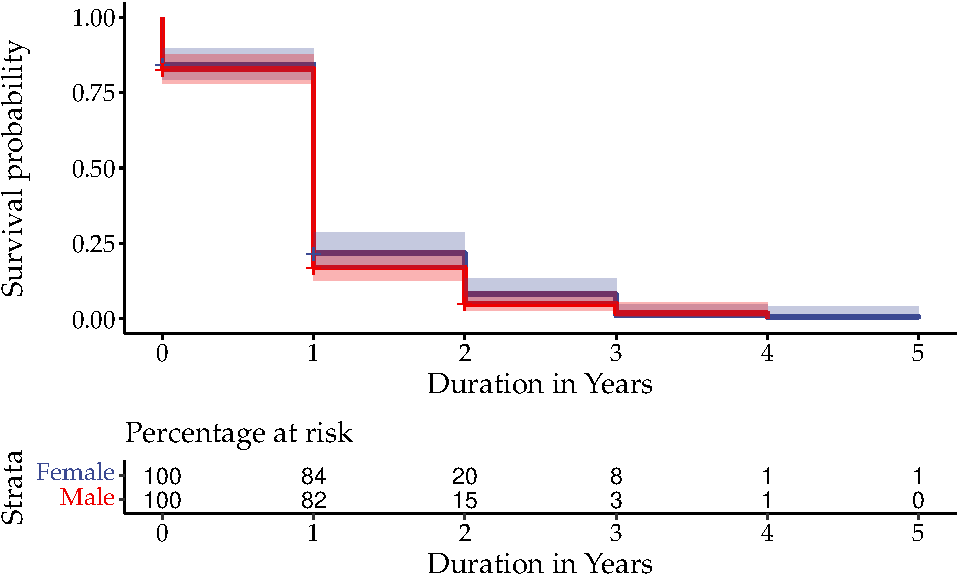
\includegraphics[width=0.75\linewidth,]{figures/fig-survival-1} \caption{Survival analysis: duration of transition to first employment}\label{fig:fig-survival}
\end{figure}

% Table created by stargazer v.5.2.3 by Marek Hlavac, Social Policy Institute. E-mail: marek.hlavac at gmail.com
% Date and time: Sun, Mar 10, 2024 - 23:49:59
\begin{table}[H] \centering 
  \caption{Odds Ratios for cluster membership (Logistic Regression)} 
  \label{tab:tbl-clusterreg} 
\scriptsize 
\begin{tabular}{@{\extracolsep{-6pt}}lcccccccc} 
\\[-1.8ex]\hline 
\hline \\[-1.8ex] 
 & \multicolumn{8}{c}{Cluster} \\ 
\cline{2-9} 
\\[-1.8ex] & TRAIN & SCHOOL & WAGE & SELF & NEET & WAGE & SELF & NEET \\ 
\\[-1.8ex] & (1) & (2) & (3) & (4) & (5) & (6) & (7) & (8)\\ 
\hline \\[-1.8ex] 
 Male (=1) & 1.00 & 1.00 & 1.00 & 1.00 & 0.04 & 1.00 & 1.00 & 0.05 \\ 
  & (28,627.00) & (28,627.00) & (28,627.00) & (28,627.00) & (0.75) & (29,118.00) & (29,118.00) & (0.79) \\ 
  Father was apprentice (=1) & 1.00 & 1.00 & 1.00 & 1.00 & 0.76$^{*}$ & 1.00 & 1.00 & 0.79$^{*}$ \\ 
  & (30,572.00) & (30,572.00) & (30,572.00) & (30,572.00) & (0.41) & (30,959.00) & (30,959.00) & (0.46) \\ 
  Father completed primary (=1) & 1.00 & 1.00 & 1.00 & 1.00 & 0.74$^{*}$ & 1.00 & 1.00 & 1.10$^{**}$ \\ 
  & (32,428.00) & (32,428.00) & (32,428.00) & (32,428.00) & (0.42) & (32,718.00) & (32,718.00) & (0.48) \\ 
  Father completed secondary (=1) & 1.00 & 1.00 & 1.00 & 1.00 & 0.86 & 1.00 & 1.00 & 3.70$^{***}$ \\ 
  & (42,113.00) & (42,113.00) & (42,113.00) & (42,113.00) & (0.61) & (42,931.00) & (42,931.00) & (0.75) \\ 
  Mother was apprentice (=1) & 1.00 & 1.00 & 1.00 & 1.00 & 0.11 & 1.00 & 1.00 & 0.08 \\ 
  & (38,545.00) & (38,545.00) & (38,545.00) & (38,545.00) & (1.10) & (38,793.00) & (38,793.00) & (1.20) \\ 
  Mother completed primary (=1) & 1.00 & 1.00 & 1.00 & 1.00 & 1.30$^{***}$ & 1.00 & 1.00 & 1.50$^{***}$ \\ 
  & (36,400.00) & (36,400.00) & (36,400.00) & (36,400.00) & (0.48) & (36,748.00) & (36,748.00) & (0.56) \\ 
  Mother completed secondary (=1) & 1.00 & 1.00 & 1.00 & 1.00 & 0.0000 & 1.00 & 1.00 & 0.0000 \\ 
  & (65,556.00) & (65,556.00) & (65,556.00) & (65,556.00) & (906.00) & (66,314.00) & (66,314.00) & (2,162.00) \\ 
  Married (=1) & 1.00 & 1.00 & 1.00 & 1.00 & 5.40$^{***}$ & 1.00 & 1.00 & 3.80$^{***}$ \\ 
  & (38,233.00) & (38,233.00) & (38,233.00) & (38,233.00) & (0.36) & (40,145.00) & (40,145.00) & (0.44) \\ 
  Beninese (=1) & 1.00 & 1.00 & 1.00 & 1.00 & 0.43 & 1.00 & 1.00 & 0.93 \\ 
  & (101,972.00) & (101,972.00) & (101,972.00) & (101,972.00) & (0.94) & (103,483.00) & (103,483.00) & (1.00) \\ 
  Ethnicity: Fon (=1) & 1.00 & 1.00 & 1.00 & 1.00 & 1.50$^{***}$ & 1.00 & 1.00 & 1.80$^{***}$ \\ 
  & (31,806.00) & (31,806.00) & (31,806.00) & (31,806.00) & (0.42) & (32,004.00) & (32,004.00) & (0.50) \\ 
  Religion: Christian (=1) & 1.00 & 1.00 & 1.00 & 1.00 & 0.35 & 1.00 & 1.00 & 0.37 \\ 
  & (39,511.00) & (39,511.00) & (39,511.00) & (39,511.00) & (0.49) & (39,773.00) & (39,773.00) & (0.56) \\ 
  Grew up in a city (=1) & 1.00 & 1.00 & 1.00 & 1.00 & 0.93$^{**}$ & 1.00 & 1.00 & 1.50$^{***}$ \\ 
  & (29,456.00) & (29,456.00) & (29,456.00) & (29,456.00) & (0.37) & (29,696.00) & (29,696.00) & (0.43) \\ 
  Years of Schooling &  &  &  &  &  & 1.00 & 1.00 & 0.92$^{***}$ \\ 
  &  &  &  &  &  & (6,676.00) & (6,676.00) & (0.09) \\ 
  Completed apprenticeship (=1) &  &  &  &  &  & 1.00 & 1.00 & 0.59 \\ 
  &  &  &  &  &  & (38,352.00) & (38,352.00) & (0.48) \\ 
  Primary school diploma: CEP (=1) &  &  &  &  &  & 1.00 & 1.00 & 0.82 \\ 
  &  &  &  &  &  & (65,364.00) & (65,364.00) & (0.71) \\ 
  Junior high diploma: BEPC (=1) &  &  &  &  &  & 1.00 & 1.00 & 0.13 \\ 
  &  &  &  &  &  & (47,349.00) & (47,349.00) & (0.70) \\ 
  Baccalauréat: BAC (=1) &  &  &  &  &  & 1.00 & 1.00 & 0.24 \\ 
  &  &  &  &  &  & (40,835.00) & (40,835.00) & (1.20) \\ 
  Lower vocational: CAP (=1) &  &  &  &  &  & 1.00 & 1.00 & 0.0000 \\ 
  &  &  &  &  &  & (64,801.00) & (64,801.00) & (2,526.00) \\ 
  2nd cycle university: Licence (=1) &  &  &  &  &  & 1.00 & 1.00 & 0.0000 \\ 
  &  &  &  &  &  & (45,100.00) & (45,100.00) & (1,371.00) \\ 
  3rd cycle university: Maîtrise (=1) &  &  &  &  &  & 1.00 & 1.00 & 0.0000 \\ 
  &  &  &  &  &  & (92,931.00) & (92,931.00) & (3,395.00) \\ 
  Constant & 0.00 & 0.00 & 0.00 & 0.00 & 0.55 & 0.00 & 0.00 & 0.89 \\ 
  & (107,481.00) & (107,481.00) & (107,481.00) & (107,481.00) & (0.97) & (115,720.00) & (115,720.00) & (1.10) \\ 
 \hline \\[-1.8ex] 
Observations & 667 & 667 & 667 & 667 & 667 & 667 & 667 & 667 \\ 
Log Likelihood & $-$0.00 & $-$0.00 & $-$0.00 & $-$0.00 & $-$112.00 & $-$0.00 & $-$0.00 & $-$84.00 \\ 
Akaike Inf. Crit. & 26.00 & 26.00 & 26.00 & 26.00 & 249.00 & 42.00 & 42.00 & 211.00 \\ 
\hline 
\hline \\[-1.8ex] 
\multicolumn{9}{l}{$^{*}$p$<$0.1; $^{**}$p$<$0.05; $^{***}$p$<$0.01} \\ 
\multicolumn{9}{l}{\textit{Notes:} Odds ratios reported.} \\ 
\end{tabular} 
\end{table} 
\begin{table}[H]

\caption{\label{tab:tbl-wage}Summary Statistics - Wage Employed}
\centering
\begin{threeparttable}
\fontsize{9}{11}\selectfont
\begin{tabular}[t]{l>{\centering\arraybackslash}p{4em}>{\centering\arraybackslash}p{4em}>{\centering\arraybackslash}p{4em}>{\centering\arraybackslash}p{4em}>{\centering\arraybackslash}p{4em}>{\centering\arraybackslash}p{4em}>{\centering\arraybackslash}p{4em}}
\toprule
\textbf{Characteristic} & \textbf{Overall} & \textbf{Female} & \textbf{Male} & \textbf{19-21} & \textbf{22-24} & \textbf{25-27} & \textbf{28-30}\\
\midrule
N & 168 & 77 & 91 & 18 & 47 & 72 & 31\\
Working arrangement &  &  &  &  &  &  & \\
\hspace{1em}One employer, regular basis & 44\% & 55\% & 34\% & 47\% & 33\% & 46\% & 52\%\\
\hspace{1em}One employer, irregular basis & 41\% & 38\% & 44\% & 41\% & 50\% & 39\% & 32\%\\
\hspace{1em}Multiple employers, irregular & 12\% & 4.1\% & 18\% & 12\% & 15\% & 9.9\% & 9.7\%\\
\hspace{1em}Family worker & 3.6\% & 2.7\% & 4.4\% & 0\% & 2.2\% & 4.2\% & 6.5\%\\
Number of workers¹ & 3.96 & 3.71 & 4.16 & 3.56 & 3.77 & 4.22 & 3.87\\
Months worked² & 7.9 & 8.2 & 7.7 & 4.4 & 7.2 & 8.8 & 8.8\\
Wage (previous month) &  &  &  &  &  &  & \\
\hspace{1em}<35,000 FCFA & 28\% & 32\% & 25\% & 40\% & 29\% & 29\% & 20\%\\
\hspace{1em}35,000-54,999 FCFA & 38\% & 39\% & 38\% & 30\% & 46\% & 38\% & 30\%\\
\hspace{1em}55,000-149.999 FCFA & 30\% & 26\% & 34\% & 30\% & 21\% & 29\% & 45\%\\
\hspace{1em}>150,000 FCFA & 3.6\% & 3.5\% & 3.8\% & 0\% & 3.6\% & 3.8\% & 5.0\%\\
Job satisfaction (out of 5)³ & 3.46 & 3.47 & 3.46 & 3.50 & 3.36 & 3.53 & 3.45\\
Life satisfaction (out of 5)³ & 3.52 & 3.61 & 3.45 & 3.61 & 3.34 & 3.61 & 3.55\\
Actively looking for new job & 65\% & 58\% & 70\% & 67\% & 66\% & 62\% & 68\%\\
\bottomrule
\end{tabular}
\begin{tablenotes}
\item \textit{Notes:} Calculated using responses from baseline survey.
\item[1] Primary employer. Includes surveyed worker.
\item[2] Of past 12 months.
\item[3] Likert scale, 1 = Very dissatisfied, 5 = Very satisfied.
\end{tablenotes}
\end{threeparttable}
\end{table}
\begin{table}[H]

\caption{\label{tab:tbl-self}Summary Statistics - Self-Employed}
\centering
\begin{threeparttable}
\fontsize{9}{11}\selectfont
\begin{tabular}[t]{l>{\centering\arraybackslash}p{4em}>{\centering\arraybackslash}p{4em}>{\centering\arraybackslash}p{4em}>{\centering\arraybackslash}p{4em}>{\centering\arraybackslash}p{4em}>{\centering\arraybackslash}p{4em}>{\centering\arraybackslash}p{4em}}
\toprule
\textbf{Characteristic} & \textbf{Overall} & \textbf{Female} & \textbf{Male} & \textbf{19-21} & \textbf{22-24} & \textbf{25-27} & \textbf{28-30}\\
\midrule
N & 119 & 61 & 58 & 14 & 39 & 45 & 21\\
Registered business¹ & 18\% & 6.2\% & 29\% & 0\% & 21\% & 19\% & 18\%\\
Pays taxes² & 13\% & 6.6\% & 19\% & 0\% & 2.6\% & 24\% & 14\%\\
Trade association member & 7.6\% & 3.3\% & 12\% & 0\% & 7.7\% & 8.9\% & 9.5\%\\
Works alone (no employees) & 72\% & 84\% & 60\% & 79\% & 72\% & 71\% & 71\%\\
Number of employees³ & 3.5 & 1.4 & 4.3 & 1.0 & 5.4 & 2.9 & 2.3\\
Months worked of past 12 & 10.00 & 9.40 & 10.26 & 7.33 & 9.91 & 9.77 & 12.00\\
Profits (previous month) &  &  &  &  &  &  & \\
\hspace{1em}<20,000 FCFA & 56\% & 67\% & 44\% & 71\% & 42\% & 61\% & 53\%\\
\hspace{1em}20,000-39,999 FCFA & 19\% & 20\% & 19\% & 21\% & 19\% & 14\% & 32\%\\
\hspace{1em}40,000-124.999 FCFA & 21\% & 13\% & 30\% & 7.1\% & 35\% & 18\% & 16\%\\
\hspace{1em}>125,000 FCFA & 3.7\% & 0\% & 7.4\% & 0\% & 3.2\% & 6.8\% & 0\%\\
Apprentices trained & 0.52 & 0.12 & 1.12 & 0.00 & 0.27 & 0.69 & 0.89\\
Job Satisfaction (out of 5, Likert scale) & 3.68 & 3.48 & 3.90 & 3.36 & 3.59 & 3.78 & 3.86\\
Life satisfaction (out of 5, Likert scale) & 3.40 & 3.18 & 3.64 & 3.36 & 3.26 & 3.58 & 3.33\\
Looking for new job & 39\% & 41\% & 36\% & 64\% & 38\% & 38\% & 24\%\\
\bottomrule
\end{tabular}
\begin{tablenotes}
\item \textit{Notes:} Calculated using responses from baseline survey.
\item[1] Either registered with Benin Chamber of Commerce and Industry (CCIB), Register of Commerce and Personal Property Transaction (RCCM), National Social Security Fund (CNSS) or National Institute of Statistics and Economic Analysis (INSAE) or in possession of a professional card (carte professionnelle de commerçant, CPC) or a Unique Fiscal Identifier (IFU).
\item[2] Paying either Synthetic Professional Tax (Taxe Professionnelle Synthètique, TPS), taxes for public space usage (e.g. patente foraine), or any other local taxes.
\item[3] Not including the business owner (i.e. the survey respondent)).
\end{tablenotes}
\end{threeparttable}
\end{table}
\begin{table}[H]

\caption{\label{tab:tbl-aspirations}Youth Aspirations}
\centering
\begin{threeparttable}
\fontsize{9}{11}\selectfont
\begin{tabular}[t]{l>{\centering\arraybackslash}p{8em}>{\centering\arraybackslash}p{8em}>{\centering\arraybackslash}p{8em}}
\toprule
  & \textbf{NEET}\newline N=238 & \textbf{Self-Employed}\newline N=119 & \textbf{Employed}\newline N=168\\
\midrule
Where do you see yourself in five years? &  &  & \\
\hspace{1em}Still looking for work & 3.0\% & - & -\\
\hspace{1em}Working for same employer & - & - & 11\%\\
\hspace{1em}Different/new employer & 24\% & 29\% & 27\%\\
\hspace{1em}(Still) self-employed & 67\% & 58\% & 48\%\\
\hspace{1em}In education/training & 3.8\% & 2.5\% & 8.9\%\\
\hspace{1em}Other & 2.1\% & 11\% & 4.8\%\\
\bottomrule
\end{tabular}
\begin{tablenotes}
\item \textit{Notes:} Calculated using responses from baseline survey.
\end{tablenotes}
\end{threeparttable}
\end{table}
\end{singlespacing}

\newpage

\hypertarget{survey-appendix-b}{%
\section*{Appendix B3}\label{survey-appendix-b}}
\addcontentsline{toc}{section}{Appendix B3}

\markboth{Appendix B3}{Appendix B3}

\setcounter{table}{0}
\renewcommand{\thetable}{B3.\arabic{table}}

\begin{singlespacing}

\providecommand{\docline}[3]{\noalign{\global\setlength{\arrayrulewidth}{#1}}\arrayrulecolor[HTML]{#2}\cline{#3}}

\setlength{\tabcolsep}{0pt}

\renewcommand*{\arraystretch}{1.15}

\begin{longtable}[c]{|p{0.75in}|p{0.75in}|p{0.75in}|p{0.75in}|p{0.75in}|p{0.75in}|p{0.75in}}

\caption{\textcolor[HTML]{000000}{\fontsize{11}{13}\selectfont{\global\setmainfont{Palatino}{Activity\ transition\ matrix:\ Combined\ data,\ 2013-2021}}}}\label{tab:tbl-fullmatrix}\\

\hhline{~~~~~~~}

\multicolumn{3}{!{\color[HTML]{FFFFFF}\vrule width 0pt}>{\centering}p{\dimexpr 2.25in+4\tabcolsep+2\arrayrulewidth}}{\textcolor[HTML]{000000}{\fontsize{8}{17}\selectfont{\global\setmainfont{Times New Roman}{}}}} & \multicolumn{4}{!{\color[HTML]{FFFFFF}\vrule width 0pt}>{\centering}p{\dimexpr 3in+6\tabcolsep+3\arrayrulewidth}!{\color[HTML]{FFFFFF}\vrule width 0pt}}{\textcolor[HTML]{000000}{\fontsize{8}{17}\selectfont{\global\setmainfont{Times New Roman}{To}}}} \\

\hhline{>{\arrayrulecolor[HTML]{000000}\global\arrayrulewidth=1pt}->{\arrayrulecolor[HTML]{000000}\global\arrayrulewidth=1pt}->{\arrayrulecolor[HTML]{000000}\global\arrayrulewidth=1pt}->{\arrayrulecolor[HTML]{000000}\global\arrayrulewidth=1pt}->{\arrayrulecolor[HTML]{000000}\global\arrayrulewidth=1pt}->{\arrayrulecolor[HTML]{000000}\global\arrayrulewidth=1pt}->{\arrayrulecolor[HTML]{000000}\global\arrayrulewidth=1pt}-}



\multicolumn{1}{!{\color[HTML]{FFFFFF}\vrule width 0pt}>{\centering}p{\dimexpr 0.75in+0\tabcolsep+0\arrayrulewidth}}{\textcolor[HTML]{000000}{\fontsize{8}{17}\selectfont{\global\setmainfont{Times New Roman}{From}}}} & \multicolumn{1}{!{\color[HTML]{FFFFFF}\vrule width 0pt}>{\centering}p{\dimexpr 0.75in+0\tabcolsep+0\arrayrulewidth}}{\textcolor[HTML]{000000}{\fontsize{8}{17}\selectfont{\global\setmainfont{Times New Roman}{In\ School}}}} & \multicolumn{1}{!{\color[HTML]{FFFFFF}\vrule width 0pt}>{\centering}p{\dimexpr 0.75in+0\tabcolsep+0\arrayrulewidth}}{\textcolor[HTML]{000000}{\fontsize{8}{17}\selectfont{\global\setmainfont{Times New Roman}{NEET}}}} & \multicolumn{1}{!{\color[HTML]{FFFFFF}\vrule width 0pt}>{\centering}p{\dimexpr 0.75in+0\tabcolsep+0\arrayrulewidth}}{\textcolor[HTML]{000000}{\fontsize{8}{17}\selectfont{\global\setmainfont{Times New Roman}{Self-Employed}}}} & \multicolumn{1}{!{\color[HTML]{FFFFFF}\vrule width 0pt}>{\centering}p{\dimexpr 0.75in+0\tabcolsep+0\arrayrulewidth}}{\textcolor[HTML]{000000}{\fontsize{8}{17}\selectfont{\global\setmainfont{Times New Roman}{Employed}}}} & \multicolumn{1}{!{\color[HTML]{FFFFFF}\vrule width 0pt}>{\centering}p{\dimexpr 0.75in+0\tabcolsep+0\arrayrulewidth}}{\textcolor[HTML]{000000}{\fontsize{8}{17}\selectfont{\global\setmainfont{Times New Roman}{Apprentice}}}} & \multicolumn{1}{!{\color[HTML]{FFFFFF}\vrule width 0pt}>{\centering}p{\dimexpr 0.75in+0\tabcolsep+0\arrayrulewidth}!{\color[HTML]{FFFFFF}\vrule width 0pt}}{\textcolor[HTML]{000000}{\fontsize{8}{17}\selectfont{\global\setmainfont{Times New Roman}{Total}}}} \\

\hhline{>{\arrayrulecolor[HTML]{000000}\global\arrayrulewidth=1pt}->{\arrayrulecolor[HTML]{000000}\global\arrayrulewidth=1pt}->{\arrayrulecolor[HTML]{000000}\global\arrayrulewidth=1pt}->{\arrayrulecolor[HTML]{000000}\global\arrayrulewidth=1pt}->{\arrayrulecolor[HTML]{000000}\global\arrayrulewidth=1pt}->{\arrayrulecolor[HTML]{000000}\global\arrayrulewidth=1pt}->{\arrayrulecolor[HTML]{000000}\global\arrayrulewidth=1pt}-}\endhead



\multicolumn{7}{!{\color[HTML]{FFFFFF}\vrule width 0pt}>{\raggedright}p{\dimexpr 5.25in+12\tabcolsep+6\arrayrulewidth}!{\color[HTML]{FFFFFF}\vrule width 0pt}}{\textcolor[HTML]{000000}{\fontsize{8}{8}\selectfont{\global\setmainfont{Palatino}{\textit{Notes:\ }}}}\textcolor[HTML]{000000}{\fontsize{8}{8}\selectfont{\global\setmainfont{Palatino}{Row\ \%,\ (Column\ \%)}}}} \\

\endfoot



\multicolumn{1}{!{\color[HTML]{FFFFFF}\vrule width 0pt}>{\centering}p{\dimexpr 0.75in+0\tabcolsep+0\arrayrulewidth}}{\textcolor[HTML]{000000}{\fontsize{8}{17}\selectfont{\global\setmainfont{Times New Roman}{In\ School}}}} & \multicolumn{1}{!{\color[HTML]{FFFFFF}\vrule width 0pt}>{\centering}p{\dimexpr 0.75in+0\tabcolsep+0\arrayrulewidth}}{\textcolor[HTML]{000000}{\fontsize{8}{17}\selectfont{\global\setmainfont{Times New Roman}{85.68\%}}}\textcolor[HTML]{000000}{\fontsize{8}{17}\selectfont{\global\setmainfont{Times New Roman}{\linebreak }}}\textcolor[HTML]{000000}{\fontsize{8}{17}\selectfont{\global\setmainfont{Times New Roman}{(98.91\%)}}}} & \multicolumn{1}{!{\color[HTML]{FFFFFF}\vrule width 0pt}>{\centering}p{\dimexpr 0.75in+0\tabcolsep+0\arrayrulewidth}}{\textcolor[HTML]{000000}{\fontsize{8}{17}\selectfont{\global\setmainfont{Times New Roman}{3.85\%}}}\textcolor[HTML]{000000}{\fontsize{8}{17}\selectfont{\global\setmainfont{Times New Roman}{\linebreak }}}\textcolor[HTML]{000000}{\fontsize{8}{17}\selectfont{\global\setmainfont{Times New Roman}{(21.74\%)}}}} & \multicolumn{1}{!{\color[HTML]{FFFFFF}\vrule width 0pt}>{\centering}p{\dimexpr 0.75in+0\tabcolsep+0\arrayrulewidth}}{\textcolor[HTML]{000000}{\fontsize{8}{17}\selectfont{\global\setmainfont{Times New Roman}{2.61\%}}}\textcolor[HTML]{000000}{\fontsize{8}{17}\selectfont{\global\setmainfont{Times New Roman}{\linebreak }}}\textcolor[HTML]{000000}{\fontsize{8}{17}\selectfont{\global\setmainfont{Times New Roman}{(11.36\%)}}}} & \multicolumn{1}{!{\color[HTML]{FFFFFF}\vrule width 0pt}>{\centering}p{\dimexpr 0.75in+0\tabcolsep+0\arrayrulewidth}}{\textcolor[HTML]{000000}{\fontsize{8}{17}\selectfont{\global\setmainfont{Times New Roman}{4.92\%}}}\textcolor[HTML]{000000}{\fontsize{8}{17}\selectfont{\global\setmainfont{Times New Roman}{\linebreak }}}\textcolor[HTML]{000000}{\fontsize{8}{17}\selectfont{\global\setmainfont{Times New Roman}{(18.40\%)}}}} & \multicolumn{1}{!{\color[HTML]{FFFFFF}\vrule width 0pt}>{\centering}p{\dimexpr 0.75in+0\tabcolsep+0\arrayrulewidth}}{\textcolor[HTML]{000000}{\fontsize{8}{17}\selectfont{\global\setmainfont{Times New Roman}{2.95\%}}}\textcolor[HTML]{000000}{\fontsize{8}{17}\selectfont{\global\setmainfont{Times New Roman}{\linebreak }}}\textcolor[HTML]{000000}{\fontsize{8}{17}\selectfont{\global\setmainfont{Times New Roman}{(17.25\%)}}}} & \multicolumn{1}{!{\color[HTML]{FFFFFF}\vrule width 0pt}>{\centering}p{\dimexpr 0.75in+0\tabcolsep+0\arrayrulewidth}!{\color[HTML]{FFFFFF}\vrule width 0pt}}{\textcolor[HTML]{000000}{\fontsize{8}{17}\selectfont{\global\setmainfont{Times New Roman}{100.00\%}}}\textcolor[HTML]{000000}{\fontsize{8}{17}\selectfont{\global\setmainfont{Times New Roman}{\linebreak }}}\textcolor[HTML]{000000}{\fontsize{8}{17}\selectfont{\global\setmainfont{Times New Roman}{(167.66\%)}}}} \\





\multicolumn{1}{!{\color[HTML]{FFFFFF}\vrule width 0pt}>{\centering}p{\dimexpr 0.75in+0\tabcolsep+0\arrayrulewidth}}{\textcolor[HTML]{000000}{\fontsize{8}{17}\selectfont{\global\setmainfont{Times New Roman}{NEET}}}} & \multicolumn{1}{!{\color[HTML]{FFFFFF}\vrule width 0pt}>{\centering}p{\dimexpr 0.75in+0\tabcolsep+0\arrayrulewidth}}{\textcolor[HTML]{000000}{\fontsize{8}{17}\selectfont{\global\setmainfont{Times New Roman}{1.82\%}}}\textcolor[HTML]{000000}{\fontsize{8}{17}\selectfont{\global\setmainfont{Times New Roman}{\linebreak }}}\textcolor[HTML]{000000}{\fontsize{8}{17}\selectfont{\global\setmainfont{Times New Roman}{(0.35\%)}}}} & \multicolumn{1}{!{\color[HTML]{FFFFFF}\vrule width 0pt}>{\centering}p{\dimexpr 0.75in+0\tabcolsep+0\arrayrulewidth}}{\textcolor[HTML]{000000}{\fontsize{8}{17}\selectfont{\global\setmainfont{Times New Roman}{64.94\%}}}\textcolor[HTML]{000000}{\fontsize{8}{17}\selectfont{\global\setmainfont{Times New Roman}{\linebreak }}}\textcolor[HTML]{000000}{\fontsize{8}{17}\selectfont{\global\setmainfont{Times New Roman}{(60.39\%)}}}} & \multicolumn{1}{!{\color[HTML]{FFFFFF}\vrule width 0pt}>{\centering}p{\dimexpr 0.75in+0\tabcolsep+0\arrayrulewidth}}{\textcolor[HTML]{000000}{\fontsize{8}{17}\selectfont{\global\setmainfont{Times New Roman}{11.17\%}}}\textcolor[HTML]{000000}{\fontsize{8}{17}\selectfont{\global\setmainfont{Times New Roman}{\linebreak }}}\textcolor[HTML]{000000}{\fontsize{8}{17}\selectfont{\global\setmainfont{Times New Roman}{(8.01\%)}}}} & \multicolumn{1}{!{\color[HTML]{FFFFFF}\vrule width 0pt}>{\centering}p{\dimexpr 0.75in+0\tabcolsep+0\arrayrulewidth}}{\textcolor[HTML]{000000}{\fontsize{8}{17}\selectfont{\global\setmainfont{Times New Roman}{14.29\%}}}\textcolor[HTML]{000000}{\fontsize{8}{17}\selectfont{\global\setmainfont{Times New Roman}{\linebreak }}}\textcolor[HTML]{000000}{\fontsize{8}{17}\selectfont{\global\setmainfont{Times New Roman}{(8.80\%)}}}} & \multicolumn{1}{!{\color[HTML]{FFFFFF}\vrule width 0pt}>{\centering}p{\dimexpr 0.75in+0\tabcolsep+0\arrayrulewidth}}{\textcolor[HTML]{000000}{\fontsize{8}{17}\selectfont{\global\setmainfont{Times New Roman}{7.79\%}}}\textcolor[HTML]{000000}{\fontsize{8}{17}\selectfont{\global\setmainfont{Times New Roman}{\linebreak }}}\textcolor[HTML]{000000}{\fontsize{8}{17}\selectfont{\global\setmainfont{Times New Roman}{(7.50\%)}}}} & \multicolumn{1}{!{\color[HTML]{FFFFFF}\vrule width 0pt}>{\centering}p{\dimexpr 0.75in+0\tabcolsep+0\arrayrulewidth}!{\color[HTML]{FFFFFF}\vrule width 0pt}}{\textcolor[HTML]{000000}{\fontsize{8}{17}\selectfont{\global\setmainfont{Times New Roman}{100.00\%}}}\textcolor[HTML]{000000}{\fontsize{8}{17}\selectfont{\global\setmainfont{Times New Roman}{\linebreak }}}\textcolor[HTML]{000000}{\fontsize{8}{17}\selectfont{\global\setmainfont{Times New Roman}{(85.04\%)}}}} \\





\multicolumn{1}{!{\color[HTML]{FFFFFF}\vrule width 0pt}>{\centering}p{\dimexpr 0.75in+0\tabcolsep+0\arrayrulewidth}}{\textcolor[HTML]{000000}{\fontsize{8}{17}\selectfont{\global\setmainfont{Times New Roman}{Self-Employed}}}} & \multicolumn{1}{!{\color[HTML]{FFFFFF}\vrule width 0pt}>{\centering}p{\dimexpr 0.75in+0\tabcolsep+0\arrayrulewidth}}{\textcolor[HTML]{000000}{\fontsize{8}{17}\selectfont{\global\setmainfont{Times New Roman}{1.87\%}}}\textcolor[HTML]{000000}{\fontsize{8}{17}\selectfont{\global\setmainfont{Times New Roman}{\linebreak }}}\textcolor[HTML]{000000}{\fontsize{8}{17}\selectfont{\global\setmainfont{Times New Roman}{(0.39\%)}}}} & \multicolumn{1}{!{\color[HTML]{FFFFFF}\vrule width 0pt}>{\centering}p{\dimexpr 0.75in+0\tabcolsep+0\arrayrulewidth}}{\textcolor[HTML]{000000}{\fontsize{8}{17}\selectfont{\global\setmainfont{Times New Roman}{4.68\%}}}\textcolor[HTML]{000000}{\fontsize{8}{17}\selectfont{\global\setmainfont{Times New Roman}{\linebreak }}}\textcolor[HTML]{000000}{\fontsize{8}{17}\selectfont{\global\setmainfont{Times New Roman}{(4.83\%)}}}} & \multicolumn{1}{!{\color[HTML]{FFFFFF}\vrule width 0pt}>{\centering}p{\dimexpr 0.75in+0\tabcolsep+0\arrayrulewidth}}{\textcolor[HTML]{000000}{\fontsize{8}{17}\selectfont{\global\setmainfont{Times New Roman}{87.82\%}}}\textcolor[HTML]{000000}{\fontsize{8}{17}\selectfont{\global\setmainfont{Times New Roman}{\linebreak }}}\textcolor[HTML]{000000}{\fontsize{8}{17}\selectfont{\global\setmainfont{Times New Roman}{(69.83\%)}}}} & \multicolumn{1}{!{\color[HTML]{FFFFFF}\vrule width 0pt}>{\centering}p{\dimexpr 0.75in+0\tabcolsep+0\arrayrulewidth}}{\textcolor[HTML]{000000}{\fontsize{8}{17}\selectfont{\global\setmainfont{Times New Roman}{3.75\%}}}\textcolor[HTML]{000000}{\fontsize{8}{17}\selectfont{\global\setmainfont{Times New Roman}{\linebreak }}}\textcolor[HTML]{000000}{\fontsize{8}{17}\selectfont{\global\setmainfont{Times New Roman}{(2.56\%)}}}} & \multicolumn{1}{!{\color[HTML]{FFFFFF}\vrule width 0pt}>{\centering}p{\dimexpr 0.75in+0\tabcolsep+0\arrayrulewidth}}{\textcolor[HTML]{000000}{\fontsize{8}{17}\selectfont{\global\setmainfont{Times New Roman}{1.87\%}}}\textcolor[HTML]{000000}{\fontsize{8}{17}\selectfont{\global\setmainfont{Times New Roman}{\linebreak }}}\textcolor[HTML]{000000}{\fontsize{8}{17}\selectfont{\global\setmainfont{Times New Roman}{(2.00\%)}}}} & \multicolumn{1}{!{\color[HTML]{FFFFFF}\vrule width 0pt}>{\centering}p{\dimexpr 0.75in+0\tabcolsep+0\arrayrulewidth}!{\color[HTML]{FFFFFF}\vrule width 0pt}}{\textcolor[HTML]{000000}{\fontsize{8}{17}\selectfont{\global\setmainfont{Times New Roman}{100.00\%}}}\textcolor[HTML]{000000}{\fontsize{8}{17}\selectfont{\global\setmainfont{Times New Roman}{\linebreak }}}\textcolor[HTML]{000000}{\fontsize{8}{17}\selectfont{\global\setmainfont{Times New Roman}{(79.62\%)}}}} \\





\multicolumn{1}{!{\color[HTML]{FFFFFF}\vrule width 0pt}>{\centering}p{\dimexpr 0.75in+0\tabcolsep+0\arrayrulewidth}}{\textcolor[HTML]{000000}{\fontsize{8}{17}\selectfont{\global\setmainfont{Times New Roman}{Employed}}}} & \multicolumn{1}{!{\color[HTML]{FFFFFF}\vrule width 0pt}>{\centering}p{\dimexpr 0.75in+0\tabcolsep+0\arrayrulewidth}}{\textcolor[HTML]{000000}{\fontsize{8}{17}\selectfont{\global\setmainfont{Times New Roman}{1.28\%}}}\textcolor[HTML]{000000}{\fontsize{8}{17}\selectfont{\global\setmainfont{Times New Roman}{\linebreak }}}\textcolor[HTML]{000000}{\fontsize{8}{17}\selectfont{\global\setmainfont{Times New Roman}{(0.30\%)}}}} & \multicolumn{1}{!{\color[HTML]{FFFFFF}\vrule width 0pt}>{\centering}p{\dimexpr 0.75in+0\tabcolsep+0\arrayrulewidth}}{\textcolor[HTML]{000000}{\fontsize{8}{17}\selectfont{\global\setmainfont{Times New Roman}{7.23\%}}}\textcolor[HTML]{000000}{\fontsize{8}{17}\selectfont{\global\setmainfont{Times New Roman}{\linebreak }}}\textcolor[HTML]{000000}{\fontsize{8}{17}\selectfont{\global\setmainfont{Times New Roman}{(8.21\%)}}}} & \multicolumn{1}{!{\color[HTML]{FFFFFF}\vrule width 0pt}>{\centering}p{\dimexpr 0.75in+0\tabcolsep+0\arrayrulewidth}}{\textcolor[HTML]{000000}{\fontsize{8}{17}\selectfont{\global\setmainfont{Times New Roman}{4.68\%}}}\textcolor[HTML]{000000}{\fontsize{8}{17}\selectfont{\global\setmainfont{Times New Roman}{\linebreak }}}\textcolor[HTML]{000000}{\fontsize{8}{17}\selectfont{\global\setmainfont{Times New Roman}{(4.10\%)}}}} & \multicolumn{1}{!{\color[HTML]{FFFFFF}\vrule width 0pt}>{\centering}p{\dimexpr 0.75in+0\tabcolsep+0\arrayrulewidth}}{\textcolor[HTML]{000000}{\fontsize{8}{17}\selectfont{\global\setmainfont{Times New Roman}{84.89\%}}}\textcolor[HTML]{000000}{\fontsize{8}{17}\selectfont{\global\setmainfont{Times New Roman}{\linebreak }}}\textcolor[HTML]{000000}{\fontsize{8}{17}\selectfont{\global\setmainfont{Times New Roman}{(63.84\%)}}}} & \multicolumn{1}{!{\color[HTML]{FFFFFF}\vrule width 0pt}>{\centering}p{\dimexpr 0.75in+0\tabcolsep+0\arrayrulewidth}}{\textcolor[HTML]{000000}{\fontsize{8}{17}\selectfont{\global\setmainfont{Times New Roman}{1.91\%}}}\textcolor[HTML]{000000}{\fontsize{8}{17}\selectfont{\global\setmainfont{Times New Roman}{\linebreak }}}\textcolor[HTML]{000000}{\fontsize{8}{17}\selectfont{\global\setmainfont{Times New Roman}{(2.25\%)}}}} & \multicolumn{1}{!{\color[HTML]{FFFFFF}\vrule width 0pt}>{\centering}p{\dimexpr 0.75in+0\tabcolsep+0\arrayrulewidth}!{\color[HTML]{FFFFFF}\vrule width 0pt}}{\textcolor[HTML]{000000}{\fontsize{8}{17}\selectfont{\global\setmainfont{Times New Roman}{100.00\%}}}\textcolor[HTML]{000000}{\fontsize{8}{17}\selectfont{\global\setmainfont{Times New Roman}{\linebreak }}}\textcolor[HTML]{000000}{\fontsize{8}{17}\selectfont{\global\setmainfont{Times New Roman}{(78.70\%)}}}} \\





\multicolumn{1}{!{\color[HTML]{FFFFFF}\vrule width 0pt}>{\centering}p{\dimexpr 0.75in+0\tabcolsep+0\arrayrulewidth}}{\textcolor[HTML]{000000}{\fontsize{8}{17}\selectfont{\global\setmainfont{Times New Roman}{Apprentice}}}} & \multicolumn{1}{!{\color[HTML]{FFFFFF}\vrule width 0pt}>{\centering}p{\dimexpr 0.75in+0\tabcolsep+0\arrayrulewidth}}{\textcolor[HTML]{000000}{\fontsize{8}{17}\selectfont{\global\setmainfont{Times New Roman}{0.26\%}}}\textcolor[HTML]{000000}{\fontsize{8}{17}\selectfont{\global\setmainfont{Times New Roman}{\linebreak }}}\textcolor[HTML]{000000}{\fontsize{8}{17}\selectfont{\global\setmainfont{Times New Roman}{(0.05\%)}}}} & \multicolumn{1}{!{\color[HTML]{FFFFFF}\vrule width 0pt}>{\centering}p{\dimexpr 0.75in+0\tabcolsep+0\arrayrulewidth}}{\textcolor[HTML]{000000}{\fontsize{8}{17}\selectfont{\global\setmainfont{Times New Roman}{5.25\%}}}\textcolor[HTML]{000000}{\fontsize{8}{17}\selectfont{\global\setmainfont{Times New Roman}{\linebreak }}}\textcolor[HTML]{000000}{\fontsize{8}{17}\selectfont{\global\setmainfont{Times New Roman}{(4.83\%)}}}} & \multicolumn{1}{!{\color[HTML]{FFFFFF}\vrule width 0pt}>{\centering}p{\dimexpr 0.75in+0\tabcolsep+0\arrayrulewidth}}{\textcolor[HTML]{000000}{\fontsize{8}{17}\selectfont{\global\setmainfont{Times New Roman}{9.45\%}}}\textcolor[HTML]{000000}{\fontsize{8}{17}\selectfont{\global\setmainfont{Times New Roman}{\linebreak }}}\textcolor[HTML]{000000}{\fontsize{8}{17}\selectfont{\global\setmainfont{Times New Roman}{(6.70\%)}}}} & \multicolumn{1}{!{\color[HTML]{FFFFFF}\vrule width 0pt}>{\centering}p{\dimexpr 0.75in+0\tabcolsep+0\arrayrulewidth}}{\textcolor[HTML]{000000}{\fontsize{8}{17}\selectfont{\global\setmainfont{Times New Roman}{10.50\%}}}\textcolor[HTML]{000000}{\fontsize{8}{17}\selectfont{\global\setmainfont{Times New Roman}{\linebreak }}}\textcolor[HTML]{000000}{\fontsize{8}{17}\selectfont{\global\setmainfont{Times New Roman}{(6.40\%)}}}} & \multicolumn{1}{!{\color[HTML]{FFFFFF}\vrule width 0pt}>{\centering}p{\dimexpr 0.75in+0\tabcolsep+0\arrayrulewidth}}{\textcolor[HTML]{000000}{\fontsize{8}{17}\selectfont{\global\setmainfont{Times New Roman}{74.54\%}}}\textcolor[HTML]{000000}{\fontsize{8}{17}\selectfont{\global\setmainfont{Times New Roman}{\linebreak }}}\textcolor[HTML]{000000}{\fontsize{8}{17}\selectfont{\global\setmainfont{Times New Roman}{(71.00\%)}}}} & \multicolumn{1}{!{\color[HTML]{FFFFFF}\vrule width 0pt}>{\centering}p{\dimexpr 0.75in+0\tabcolsep+0\arrayrulewidth}!{\color[HTML]{FFFFFF}\vrule width 0pt}}{\textcolor[HTML]{000000}{\fontsize{8}{17}\selectfont{\global\setmainfont{Times New Roman}{100.00\%}}}\textcolor[HTML]{000000}{\fontsize{8}{17}\selectfont{\global\setmainfont{Times New Roman}{\linebreak }}}\textcolor[HTML]{000000}{\fontsize{8}{17}\selectfont{\global\setmainfont{Times New Roman}{(88.98\%)}}}} \\





\multicolumn{1}{!{\color[HTML]{FFFFFF}\vrule width 0pt}>{\centering}p{\dimexpr 0.75in+0\tabcolsep+0\arrayrulewidth}}{\textcolor[HTML]{000000}{\fontsize{8}{17}\selectfont{\global\setmainfont{Times New Roman}{Total}}}} & \multicolumn{1}{!{\color[HTML]{FFFFFF}\vrule width 0pt}>{\centering}p{\dimexpr 0.75in+0\tabcolsep+0\arrayrulewidth}}{\textcolor[HTML]{000000}{\fontsize{8}{17}\selectfont{\global\setmainfont{Times New Roman}{90.91\%}}}\textcolor[HTML]{000000}{\fontsize{8}{17}\selectfont{\global\setmainfont{Times New Roman}{\linebreak }}}\textcolor[HTML]{000000}{\fontsize{8}{17}\selectfont{\global\setmainfont{Times New Roman}{(100.00\%)}}}} & \multicolumn{1}{!{\color[HTML]{FFFFFF}\vrule width 0pt}>{\centering}p{\dimexpr 0.75in+0\tabcolsep+0\arrayrulewidth}}{\textcolor[HTML]{000000}{\fontsize{8}{17}\selectfont{\global\setmainfont{Times New Roman}{85.95\%}}}\textcolor[HTML]{000000}{\fontsize{8}{17}\selectfont{\global\setmainfont{Times New Roman}{\linebreak }}}\textcolor[HTML]{000000}{\fontsize{8}{17}\selectfont{\global\setmainfont{Times New Roman}{(100.00\%)}}}} & \multicolumn{1}{!{\color[HTML]{FFFFFF}\vrule width 0pt}>{\centering}p{\dimexpr 0.75in+0\tabcolsep+0\arrayrulewidth}}{\textcolor[HTML]{000000}{\fontsize{8}{17}\selectfont{\global\setmainfont{Times New Roman}{115.73\%}}}\textcolor[HTML]{000000}{\fontsize{8}{17}\selectfont{\global\setmainfont{Times New Roman}{\linebreak }}}\textcolor[HTML]{000000}{\fontsize{8}{17}\selectfont{\global\setmainfont{Times New Roman}{(100.00\%)}}}} & \multicolumn{1}{!{\color[HTML]{FFFFFF}\vrule width 0pt}>{\centering}p{\dimexpr 0.75in+0\tabcolsep+0\arrayrulewidth}}{\textcolor[HTML]{000000}{\fontsize{8}{17}\selectfont{\global\setmainfont{Times New Roman}{118.34\%}}}\textcolor[HTML]{000000}{\fontsize{8}{17}\selectfont{\global\setmainfont{Times New Roman}{\linebreak }}}\textcolor[HTML]{000000}{\fontsize{8}{17}\selectfont{\global\setmainfont{Times New Roman}{(100.00\%)}}}} & \multicolumn{1}{!{\color[HTML]{FFFFFF}\vrule width 0pt}>{\centering}p{\dimexpr 0.75in+0\tabcolsep+0\arrayrulewidth}}{\textcolor[HTML]{000000}{\fontsize{8}{17}\selectfont{\global\setmainfont{Times New Roman}{89.07\%}}}\textcolor[HTML]{000000}{\fontsize{8}{17}\selectfont{\global\setmainfont{Times New Roman}{\linebreak }}}\textcolor[HTML]{000000}{\fontsize{8}{17}\selectfont{\global\setmainfont{Times New Roman}{(100.00\%)}}}} & \multicolumn{1}{!{\color[HTML]{FFFFFF}\vrule width 0pt}>{\centering}p{\dimexpr 0.75in+0\tabcolsep+0\arrayrulewidth}!{\color[HTML]{FFFFFF}\vrule width 0pt}}{\textcolor[HTML]{000000}{\fontsize{8}{17}\selectfont{\global\setmainfont{Times New Roman}{}}}} \\

\hhline{>{\arrayrulecolor[HTML]{000000}\global\arrayrulewidth=1pt}->{\arrayrulecolor[HTML]{000000}\global\arrayrulewidth=1pt}->{\arrayrulecolor[HTML]{000000}\global\arrayrulewidth=1pt}->{\arrayrulecolor[HTML]{000000}\global\arrayrulewidth=1pt}->{\arrayrulecolor[HTML]{000000}\global\arrayrulewidth=1pt}->{\arrayrulecolor[HTML]{000000}\global\arrayrulewidth=1pt}->{\arrayrulecolor[HTML]{000000}\global\arrayrulewidth=1pt}-}



\end{longtable}

\newpage


\providecommand{\docline}[3]{\noalign{\global\setlength{\arrayrulewidth}{#1}}\arrayrulecolor[HTML]{#2}\cline{#3}}

\setlength{\tabcolsep}{0pt}

\renewcommand*{\arraystretch}{1.15}

\begin{longtable}[c]{|p{0.75in}|p{0.75in}|p{0.75in}|p{0.75in}|p{0.75in}|p{0.75in}|p{0.75in}}

\caption{\textcolor[HTML]{000000}{\fontsize{11}{13}\selectfont{\global\setmainfont{Palatino}{Activity\ transition\ matrix:\ Event\ History,\ 2013-2019}}}}\label{tab:tbl-historymatrix}\\

\hhline{~~~~~~~}

\multicolumn{3}{!{\color[HTML]{FFFFFF}\vrule width 0pt}>{\centering}p{\dimexpr 2.25in+4\tabcolsep+2\arrayrulewidth}}{\textcolor[HTML]{000000}{\fontsize{8}{17}\selectfont{\global\setmainfont{Times New Roman}{}}}} & \multicolumn{4}{!{\color[HTML]{FFFFFF}\vrule width 0pt}>{\centering}p{\dimexpr 3in+6\tabcolsep+3\arrayrulewidth}!{\color[HTML]{FFFFFF}\vrule width 0pt}}{\textcolor[HTML]{000000}{\fontsize{8}{17}\selectfont{\global\setmainfont{Times New Roman}{To}}}} \\

\hhline{>{\arrayrulecolor[HTML]{000000}\global\arrayrulewidth=1pt}->{\arrayrulecolor[HTML]{000000}\global\arrayrulewidth=1pt}->{\arrayrulecolor[HTML]{000000}\global\arrayrulewidth=1pt}->{\arrayrulecolor[HTML]{000000}\global\arrayrulewidth=1pt}->{\arrayrulecolor[HTML]{000000}\global\arrayrulewidth=1pt}->{\arrayrulecolor[HTML]{000000}\global\arrayrulewidth=1pt}->{\arrayrulecolor[HTML]{000000}\global\arrayrulewidth=1pt}-}



\multicolumn{1}{!{\color[HTML]{FFFFFF}\vrule width 0pt}>{\centering}p{\dimexpr 0.75in+0\tabcolsep+0\arrayrulewidth}}{\textcolor[HTML]{000000}{\fontsize{8}{17}\selectfont{\global\setmainfont{Times New Roman}{From}}}} & \multicolumn{1}{!{\color[HTML]{FFFFFF}\vrule width 0pt}>{\centering}p{\dimexpr 0.75in+0\tabcolsep+0\arrayrulewidth}}{\textcolor[HTML]{000000}{\fontsize{8}{17}\selectfont{\global\setmainfont{Times New Roman}{In\ School}}}} & \multicolumn{1}{!{\color[HTML]{FFFFFF}\vrule width 0pt}>{\centering}p{\dimexpr 0.75in+0\tabcolsep+0\arrayrulewidth}}{\textcolor[HTML]{000000}{\fontsize{8}{17}\selectfont{\global\setmainfont{Times New Roman}{NEET}}}} & \multicolumn{1}{!{\color[HTML]{FFFFFF}\vrule width 0pt}>{\centering}p{\dimexpr 0.75in+0\tabcolsep+0\arrayrulewidth}}{\textcolor[HTML]{000000}{\fontsize{8}{17}\selectfont{\global\setmainfont{Times New Roman}{Self-Employed}}}} & \multicolumn{1}{!{\color[HTML]{FFFFFF}\vrule width 0pt}>{\centering}p{\dimexpr 0.75in+0\tabcolsep+0\arrayrulewidth}}{\textcolor[HTML]{000000}{\fontsize{8}{17}\selectfont{\global\setmainfont{Times New Roman}{Employed}}}} & \multicolumn{1}{!{\color[HTML]{FFFFFF}\vrule width 0pt}>{\centering}p{\dimexpr 0.75in+0\tabcolsep+0\arrayrulewidth}}{\textcolor[HTML]{000000}{\fontsize{8}{17}\selectfont{\global\setmainfont{Times New Roman}{Apprentice}}}} & \multicolumn{1}{!{\color[HTML]{FFFFFF}\vrule width 0pt}>{\centering}p{\dimexpr 0.75in+0\tabcolsep+0\arrayrulewidth}!{\color[HTML]{FFFFFF}\vrule width 0pt}}{\textcolor[HTML]{000000}{\fontsize{8}{17}\selectfont{\global\setmainfont{Times New Roman}{Total}}}} \\

\hhline{>{\arrayrulecolor[HTML]{000000}\global\arrayrulewidth=1pt}->{\arrayrulecolor[HTML]{000000}\global\arrayrulewidth=1pt}->{\arrayrulecolor[HTML]{000000}\global\arrayrulewidth=1pt}->{\arrayrulecolor[HTML]{000000}\global\arrayrulewidth=1pt}->{\arrayrulecolor[HTML]{000000}\global\arrayrulewidth=1pt}->{\arrayrulecolor[HTML]{000000}\global\arrayrulewidth=1pt}->{\arrayrulecolor[HTML]{000000}\global\arrayrulewidth=1pt}-}\endhead



\multicolumn{7}{!{\color[HTML]{FFFFFF}\vrule width 0pt}>{\raggedright}p{\dimexpr 5.25in+12\tabcolsep+6\arrayrulewidth}!{\color[HTML]{FFFFFF}\vrule width 0pt}}{\textcolor[HTML]{000000}{\fontsize{8}{8}\selectfont{\global\setmainfont{Palatino}{\textit{Notes:\ }}}}\textcolor[HTML]{000000}{\fontsize{8}{8}\selectfont{\global\setmainfont{Palatino}{Row\ \%,\ (Column\ \%)}}}} \\

\endfoot



\multicolumn{1}{!{\color[HTML]{FFFFFF}\vrule width 0pt}>{\centering}p{\dimexpr 0.75in+0\tabcolsep+0\arrayrulewidth}}{\textcolor[HTML]{000000}{\fontsize{8}{17}\selectfont{\global\setmainfont{Times New Roman}{In\ School}}}} & \multicolumn{1}{!{\color[HTML]{FFFFFF}\vrule width 0pt}>{\centering}p{\dimexpr 0.75in+0\tabcolsep+0\arrayrulewidth}}{\textcolor[HTML]{000000}{\fontsize{8}{17}\selectfont{\global\setmainfont{Times New Roman}{85.68\%}}}\textcolor[HTML]{000000}{\fontsize{8}{17}\selectfont{\global\setmainfont{Times New Roman}{\linebreak }}}\textcolor[HTML]{000000}{\fontsize{8}{17}\selectfont{\global\setmainfont{Times New Roman}{(98.91\%)}}}} & \multicolumn{1}{!{\color[HTML]{FFFFFF}\vrule width 0pt}>{\centering}p{\dimexpr 0.75in+0\tabcolsep+0\arrayrulewidth}}{\textcolor[HTML]{000000}{\fontsize{8}{17}\selectfont{\global\setmainfont{Times New Roman}{3.85\%}}}\textcolor[HTML]{000000}{\fontsize{8}{17}\selectfont{\global\setmainfont{Times New Roman}{\linebreak }}}\textcolor[HTML]{000000}{\fontsize{8}{17}\selectfont{\global\setmainfont{Times New Roman}{(21.74\%)}}}} & \multicolumn{1}{!{\color[HTML]{FFFFFF}\vrule width 0pt}>{\centering}p{\dimexpr 0.75in+0\tabcolsep+0\arrayrulewidth}}{\textcolor[HTML]{000000}{\fontsize{8}{17}\selectfont{\global\setmainfont{Times New Roman}{2.61\%}}}\textcolor[HTML]{000000}{\fontsize{8}{17}\selectfont{\global\setmainfont{Times New Roman}{\linebreak }}}\textcolor[HTML]{000000}{\fontsize{8}{17}\selectfont{\global\setmainfont{Times New Roman}{(11.36\%)}}}} & \multicolumn{1}{!{\color[HTML]{FFFFFF}\vrule width 0pt}>{\centering}p{\dimexpr 0.75in+0\tabcolsep+0\arrayrulewidth}}{\textcolor[HTML]{000000}{\fontsize{8}{17}\selectfont{\global\setmainfont{Times New Roman}{4.92\%}}}\textcolor[HTML]{000000}{\fontsize{8}{17}\selectfont{\global\setmainfont{Times New Roman}{\linebreak }}}\textcolor[HTML]{000000}{\fontsize{8}{17}\selectfont{\global\setmainfont{Times New Roman}{(18.40\%)}}}} & \multicolumn{1}{!{\color[HTML]{FFFFFF}\vrule width 0pt}>{\centering}p{\dimexpr 0.75in+0\tabcolsep+0\arrayrulewidth}}{\textcolor[HTML]{000000}{\fontsize{8}{17}\selectfont{\global\setmainfont{Times New Roman}{2.95\%}}}\textcolor[HTML]{000000}{\fontsize{8}{17}\selectfont{\global\setmainfont{Times New Roman}{\linebreak }}}\textcolor[HTML]{000000}{\fontsize{8}{17}\selectfont{\global\setmainfont{Times New Roman}{(17.25\%)}}}} & \multicolumn{1}{!{\color[HTML]{FFFFFF}\vrule width 0pt}>{\centering}p{\dimexpr 0.75in+0\tabcolsep+0\arrayrulewidth}!{\color[HTML]{FFFFFF}\vrule width 0pt}}{\textcolor[HTML]{000000}{\fontsize{8}{17}\selectfont{\global\setmainfont{Times New Roman}{100.00\%}}}\textcolor[HTML]{000000}{\fontsize{8}{17}\selectfont{\global\setmainfont{Times New Roman}{\linebreak }}}\textcolor[HTML]{000000}{\fontsize{8}{17}\selectfont{\global\setmainfont{Times New Roman}{(167.66\%)}}}} \\





\multicolumn{1}{!{\color[HTML]{FFFFFF}\vrule width 0pt}>{\centering}p{\dimexpr 0.75in+0\tabcolsep+0\arrayrulewidth}}{\textcolor[HTML]{000000}{\fontsize{8}{17}\selectfont{\global\setmainfont{Times New Roman}{NEET}}}} & \multicolumn{1}{!{\color[HTML]{FFFFFF}\vrule width 0pt}>{\centering}p{\dimexpr 0.75in+0\tabcolsep+0\arrayrulewidth}}{\textcolor[HTML]{000000}{\fontsize{8}{17}\selectfont{\global\setmainfont{Times New Roman}{1.82\%}}}\textcolor[HTML]{000000}{\fontsize{8}{17}\selectfont{\global\setmainfont{Times New Roman}{\linebreak }}}\textcolor[HTML]{000000}{\fontsize{8}{17}\selectfont{\global\setmainfont{Times New Roman}{(0.35\%)}}}} & \multicolumn{1}{!{\color[HTML]{FFFFFF}\vrule width 0pt}>{\centering}p{\dimexpr 0.75in+0\tabcolsep+0\arrayrulewidth}}{\textcolor[HTML]{000000}{\fontsize{8}{17}\selectfont{\global\setmainfont{Times New Roman}{64.94\%}}}\textcolor[HTML]{000000}{\fontsize{8}{17}\selectfont{\global\setmainfont{Times New Roman}{\linebreak }}}\textcolor[HTML]{000000}{\fontsize{8}{17}\selectfont{\global\setmainfont{Times New Roman}{(60.39\%)}}}} & \multicolumn{1}{!{\color[HTML]{FFFFFF}\vrule width 0pt}>{\centering}p{\dimexpr 0.75in+0\tabcolsep+0\arrayrulewidth}}{\textcolor[HTML]{000000}{\fontsize{8}{17}\selectfont{\global\setmainfont{Times New Roman}{11.17\%}}}\textcolor[HTML]{000000}{\fontsize{8}{17}\selectfont{\global\setmainfont{Times New Roman}{\linebreak }}}\textcolor[HTML]{000000}{\fontsize{8}{17}\selectfont{\global\setmainfont{Times New Roman}{(8.01\%)}}}} & \multicolumn{1}{!{\color[HTML]{FFFFFF}\vrule width 0pt}>{\centering}p{\dimexpr 0.75in+0\tabcolsep+0\arrayrulewidth}}{\textcolor[HTML]{000000}{\fontsize{8}{17}\selectfont{\global\setmainfont{Times New Roman}{14.29\%}}}\textcolor[HTML]{000000}{\fontsize{8}{17}\selectfont{\global\setmainfont{Times New Roman}{\linebreak }}}\textcolor[HTML]{000000}{\fontsize{8}{17}\selectfont{\global\setmainfont{Times New Roman}{(8.80\%)}}}} & \multicolumn{1}{!{\color[HTML]{FFFFFF}\vrule width 0pt}>{\centering}p{\dimexpr 0.75in+0\tabcolsep+0\arrayrulewidth}}{\textcolor[HTML]{000000}{\fontsize{8}{17}\selectfont{\global\setmainfont{Times New Roman}{7.79\%}}}\textcolor[HTML]{000000}{\fontsize{8}{17}\selectfont{\global\setmainfont{Times New Roman}{\linebreak }}}\textcolor[HTML]{000000}{\fontsize{8}{17}\selectfont{\global\setmainfont{Times New Roman}{(7.50\%)}}}} & \multicolumn{1}{!{\color[HTML]{FFFFFF}\vrule width 0pt}>{\centering}p{\dimexpr 0.75in+0\tabcolsep+0\arrayrulewidth}!{\color[HTML]{FFFFFF}\vrule width 0pt}}{\textcolor[HTML]{000000}{\fontsize{8}{17}\selectfont{\global\setmainfont{Times New Roman}{100.00\%}}}\textcolor[HTML]{000000}{\fontsize{8}{17}\selectfont{\global\setmainfont{Times New Roman}{\linebreak }}}\textcolor[HTML]{000000}{\fontsize{8}{17}\selectfont{\global\setmainfont{Times New Roman}{(85.04\%)}}}} \\





\multicolumn{1}{!{\color[HTML]{FFFFFF}\vrule width 0pt}>{\centering}p{\dimexpr 0.75in+0\tabcolsep+0\arrayrulewidth}}{\textcolor[HTML]{000000}{\fontsize{8}{17}\selectfont{\global\setmainfont{Times New Roman}{Self-Employed}}}} & \multicolumn{1}{!{\color[HTML]{FFFFFF}\vrule width 0pt}>{\centering}p{\dimexpr 0.75in+0\tabcolsep+0\arrayrulewidth}}{\textcolor[HTML]{000000}{\fontsize{8}{17}\selectfont{\global\setmainfont{Times New Roman}{1.87\%}}}\textcolor[HTML]{000000}{\fontsize{8}{17}\selectfont{\global\setmainfont{Times New Roman}{\linebreak }}}\textcolor[HTML]{000000}{\fontsize{8}{17}\selectfont{\global\setmainfont{Times New Roman}{(0.39\%)}}}} & \multicolumn{1}{!{\color[HTML]{FFFFFF}\vrule width 0pt}>{\centering}p{\dimexpr 0.75in+0\tabcolsep+0\arrayrulewidth}}{\textcolor[HTML]{000000}{\fontsize{8}{17}\selectfont{\global\setmainfont{Times New Roman}{4.68\%}}}\textcolor[HTML]{000000}{\fontsize{8}{17}\selectfont{\global\setmainfont{Times New Roman}{\linebreak }}}\textcolor[HTML]{000000}{\fontsize{8}{17}\selectfont{\global\setmainfont{Times New Roman}{(4.83\%)}}}} & \multicolumn{1}{!{\color[HTML]{FFFFFF}\vrule width 0pt}>{\centering}p{\dimexpr 0.75in+0\tabcolsep+0\arrayrulewidth}}{\textcolor[HTML]{000000}{\fontsize{8}{17}\selectfont{\global\setmainfont{Times New Roman}{87.82\%}}}\textcolor[HTML]{000000}{\fontsize{8}{17}\selectfont{\global\setmainfont{Times New Roman}{\linebreak }}}\textcolor[HTML]{000000}{\fontsize{8}{17}\selectfont{\global\setmainfont{Times New Roman}{(69.83\%)}}}} & \multicolumn{1}{!{\color[HTML]{FFFFFF}\vrule width 0pt}>{\centering}p{\dimexpr 0.75in+0\tabcolsep+0\arrayrulewidth}}{\textcolor[HTML]{000000}{\fontsize{8}{17}\selectfont{\global\setmainfont{Times New Roman}{3.75\%}}}\textcolor[HTML]{000000}{\fontsize{8}{17}\selectfont{\global\setmainfont{Times New Roman}{\linebreak }}}\textcolor[HTML]{000000}{\fontsize{8}{17}\selectfont{\global\setmainfont{Times New Roman}{(2.56\%)}}}} & \multicolumn{1}{!{\color[HTML]{FFFFFF}\vrule width 0pt}>{\centering}p{\dimexpr 0.75in+0\tabcolsep+0\arrayrulewidth}}{\textcolor[HTML]{000000}{\fontsize{8}{17}\selectfont{\global\setmainfont{Times New Roman}{1.87\%}}}\textcolor[HTML]{000000}{\fontsize{8}{17}\selectfont{\global\setmainfont{Times New Roman}{\linebreak }}}\textcolor[HTML]{000000}{\fontsize{8}{17}\selectfont{\global\setmainfont{Times New Roman}{(2.00\%)}}}} & \multicolumn{1}{!{\color[HTML]{FFFFFF}\vrule width 0pt}>{\centering}p{\dimexpr 0.75in+0\tabcolsep+0\arrayrulewidth}!{\color[HTML]{FFFFFF}\vrule width 0pt}}{\textcolor[HTML]{000000}{\fontsize{8}{17}\selectfont{\global\setmainfont{Times New Roman}{100.00\%}}}\textcolor[HTML]{000000}{\fontsize{8}{17}\selectfont{\global\setmainfont{Times New Roman}{\linebreak }}}\textcolor[HTML]{000000}{\fontsize{8}{17}\selectfont{\global\setmainfont{Times New Roman}{(79.62\%)}}}} \\





\multicolumn{1}{!{\color[HTML]{FFFFFF}\vrule width 0pt}>{\centering}p{\dimexpr 0.75in+0\tabcolsep+0\arrayrulewidth}}{\textcolor[HTML]{000000}{\fontsize{8}{17}\selectfont{\global\setmainfont{Times New Roman}{Employed}}}} & \multicolumn{1}{!{\color[HTML]{FFFFFF}\vrule width 0pt}>{\centering}p{\dimexpr 0.75in+0\tabcolsep+0\arrayrulewidth}}{\textcolor[HTML]{000000}{\fontsize{8}{17}\selectfont{\global\setmainfont{Times New Roman}{1.28\%}}}\textcolor[HTML]{000000}{\fontsize{8}{17}\selectfont{\global\setmainfont{Times New Roman}{\linebreak }}}\textcolor[HTML]{000000}{\fontsize{8}{17}\selectfont{\global\setmainfont{Times New Roman}{(0.30\%)}}}} & \multicolumn{1}{!{\color[HTML]{FFFFFF}\vrule width 0pt}>{\centering}p{\dimexpr 0.75in+0\tabcolsep+0\arrayrulewidth}}{\textcolor[HTML]{000000}{\fontsize{8}{17}\selectfont{\global\setmainfont{Times New Roman}{7.23\%}}}\textcolor[HTML]{000000}{\fontsize{8}{17}\selectfont{\global\setmainfont{Times New Roman}{\linebreak }}}\textcolor[HTML]{000000}{\fontsize{8}{17}\selectfont{\global\setmainfont{Times New Roman}{(8.21\%)}}}} & \multicolumn{1}{!{\color[HTML]{FFFFFF}\vrule width 0pt}>{\centering}p{\dimexpr 0.75in+0\tabcolsep+0\arrayrulewidth}}{\textcolor[HTML]{000000}{\fontsize{8}{17}\selectfont{\global\setmainfont{Times New Roman}{4.68\%}}}\textcolor[HTML]{000000}{\fontsize{8}{17}\selectfont{\global\setmainfont{Times New Roman}{\linebreak }}}\textcolor[HTML]{000000}{\fontsize{8}{17}\selectfont{\global\setmainfont{Times New Roman}{(4.10\%)}}}} & \multicolumn{1}{!{\color[HTML]{FFFFFF}\vrule width 0pt}>{\centering}p{\dimexpr 0.75in+0\tabcolsep+0\arrayrulewidth}}{\textcolor[HTML]{000000}{\fontsize{8}{17}\selectfont{\global\setmainfont{Times New Roman}{84.89\%}}}\textcolor[HTML]{000000}{\fontsize{8}{17}\selectfont{\global\setmainfont{Times New Roman}{\linebreak }}}\textcolor[HTML]{000000}{\fontsize{8}{17}\selectfont{\global\setmainfont{Times New Roman}{(63.84\%)}}}} & \multicolumn{1}{!{\color[HTML]{FFFFFF}\vrule width 0pt}>{\centering}p{\dimexpr 0.75in+0\tabcolsep+0\arrayrulewidth}}{\textcolor[HTML]{000000}{\fontsize{8}{17}\selectfont{\global\setmainfont{Times New Roman}{1.91\%}}}\textcolor[HTML]{000000}{\fontsize{8}{17}\selectfont{\global\setmainfont{Times New Roman}{\linebreak }}}\textcolor[HTML]{000000}{\fontsize{8}{17}\selectfont{\global\setmainfont{Times New Roman}{(2.25\%)}}}} & \multicolumn{1}{!{\color[HTML]{FFFFFF}\vrule width 0pt}>{\centering}p{\dimexpr 0.75in+0\tabcolsep+0\arrayrulewidth}!{\color[HTML]{FFFFFF}\vrule width 0pt}}{\textcolor[HTML]{000000}{\fontsize{8}{17}\selectfont{\global\setmainfont{Times New Roman}{100.00\%}}}\textcolor[HTML]{000000}{\fontsize{8}{17}\selectfont{\global\setmainfont{Times New Roman}{\linebreak }}}\textcolor[HTML]{000000}{\fontsize{8}{17}\selectfont{\global\setmainfont{Times New Roman}{(78.70\%)}}}} \\





\multicolumn{1}{!{\color[HTML]{FFFFFF}\vrule width 0pt}>{\centering}p{\dimexpr 0.75in+0\tabcolsep+0\arrayrulewidth}}{\textcolor[HTML]{000000}{\fontsize{8}{17}\selectfont{\global\setmainfont{Times New Roman}{Apprentice}}}} & \multicolumn{1}{!{\color[HTML]{FFFFFF}\vrule width 0pt}>{\centering}p{\dimexpr 0.75in+0\tabcolsep+0\arrayrulewidth}}{\textcolor[HTML]{000000}{\fontsize{8}{17}\selectfont{\global\setmainfont{Times New Roman}{0.26\%}}}\textcolor[HTML]{000000}{\fontsize{8}{17}\selectfont{\global\setmainfont{Times New Roman}{\linebreak }}}\textcolor[HTML]{000000}{\fontsize{8}{17}\selectfont{\global\setmainfont{Times New Roman}{(0.05\%)}}}} & \multicolumn{1}{!{\color[HTML]{FFFFFF}\vrule width 0pt}>{\centering}p{\dimexpr 0.75in+0\tabcolsep+0\arrayrulewidth}}{\textcolor[HTML]{000000}{\fontsize{8}{17}\selectfont{\global\setmainfont{Times New Roman}{5.25\%}}}\textcolor[HTML]{000000}{\fontsize{8}{17}\selectfont{\global\setmainfont{Times New Roman}{\linebreak }}}\textcolor[HTML]{000000}{\fontsize{8}{17}\selectfont{\global\setmainfont{Times New Roman}{(4.83\%)}}}} & \multicolumn{1}{!{\color[HTML]{FFFFFF}\vrule width 0pt}>{\centering}p{\dimexpr 0.75in+0\tabcolsep+0\arrayrulewidth}}{\textcolor[HTML]{000000}{\fontsize{8}{17}\selectfont{\global\setmainfont{Times New Roman}{9.45\%}}}\textcolor[HTML]{000000}{\fontsize{8}{17}\selectfont{\global\setmainfont{Times New Roman}{\linebreak }}}\textcolor[HTML]{000000}{\fontsize{8}{17}\selectfont{\global\setmainfont{Times New Roman}{(6.70\%)}}}} & \multicolumn{1}{!{\color[HTML]{FFFFFF}\vrule width 0pt}>{\centering}p{\dimexpr 0.75in+0\tabcolsep+0\arrayrulewidth}}{\textcolor[HTML]{000000}{\fontsize{8}{17}\selectfont{\global\setmainfont{Times New Roman}{10.50\%}}}\textcolor[HTML]{000000}{\fontsize{8}{17}\selectfont{\global\setmainfont{Times New Roman}{\linebreak }}}\textcolor[HTML]{000000}{\fontsize{8}{17}\selectfont{\global\setmainfont{Times New Roman}{(6.40\%)}}}} & \multicolumn{1}{!{\color[HTML]{FFFFFF}\vrule width 0pt}>{\centering}p{\dimexpr 0.75in+0\tabcolsep+0\arrayrulewidth}}{\textcolor[HTML]{000000}{\fontsize{8}{17}\selectfont{\global\setmainfont{Times New Roman}{74.54\%}}}\textcolor[HTML]{000000}{\fontsize{8}{17}\selectfont{\global\setmainfont{Times New Roman}{\linebreak }}}\textcolor[HTML]{000000}{\fontsize{8}{17}\selectfont{\global\setmainfont{Times New Roman}{(71.00\%)}}}} & \multicolumn{1}{!{\color[HTML]{FFFFFF}\vrule width 0pt}>{\centering}p{\dimexpr 0.75in+0\tabcolsep+0\arrayrulewidth}!{\color[HTML]{FFFFFF}\vrule width 0pt}}{\textcolor[HTML]{000000}{\fontsize{8}{17}\selectfont{\global\setmainfont{Times New Roman}{100.00\%}}}\textcolor[HTML]{000000}{\fontsize{8}{17}\selectfont{\global\setmainfont{Times New Roman}{\linebreak }}}\textcolor[HTML]{000000}{\fontsize{8}{17}\selectfont{\global\setmainfont{Times New Roman}{(88.98\%)}}}} \\





\multicolumn{1}{!{\color[HTML]{FFFFFF}\vrule width 0pt}>{\centering}p{\dimexpr 0.75in+0\tabcolsep+0\arrayrulewidth}}{\textcolor[HTML]{000000}{\fontsize{8}{17}\selectfont{\global\setmainfont{Times New Roman}{Total}}}} & \multicolumn{1}{!{\color[HTML]{FFFFFF}\vrule width 0pt}>{\centering}p{\dimexpr 0.75in+0\tabcolsep+0\arrayrulewidth}}{\textcolor[HTML]{000000}{\fontsize{8}{17}\selectfont{\global\setmainfont{Times New Roman}{90.91\%}}}\textcolor[HTML]{000000}{\fontsize{8}{17}\selectfont{\global\setmainfont{Times New Roman}{\linebreak }}}\textcolor[HTML]{000000}{\fontsize{8}{17}\selectfont{\global\setmainfont{Times New Roman}{(100.00\%)}}}} & \multicolumn{1}{!{\color[HTML]{FFFFFF}\vrule width 0pt}>{\centering}p{\dimexpr 0.75in+0\tabcolsep+0\arrayrulewidth}}{\textcolor[HTML]{000000}{\fontsize{8}{17}\selectfont{\global\setmainfont{Times New Roman}{85.95\%}}}\textcolor[HTML]{000000}{\fontsize{8}{17}\selectfont{\global\setmainfont{Times New Roman}{\linebreak }}}\textcolor[HTML]{000000}{\fontsize{8}{17}\selectfont{\global\setmainfont{Times New Roman}{(100.00\%)}}}} & \multicolumn{1}{!{\color[HTML]{FFFFFF}\vrule width 0pt}>{\centering}p{\dimexpr 0.75in+0\tabcolsep+0\arrayrulewidth}}{\textcolor[HTML]{000000}{\fontsize{8}{17}\selectfont{\global\setmainfont{Times New Roman}{115.73\%}}}\textcolor[HTML]{000000}{\fontsize{8}{17}\selectfont{\global\setmainfont{Times New Roman}{\linebreak }}}\textcolor[HTML]{000000}{\fontsize{8}{17}\selectfont{\global\setmainfont{Times New Roman}{(100.00\%)}}}} & \multicolumn{1}{!{\color[HTML]{FFFFFF}\vrule width 0pt}>{\centering}p{\dimexpr 0.75in+0\tabcolsep+0\arrayrulewidth}}{\textcolor[HTML]{000000}{\fontsize{8}{17}\selectfont{\global\setmainfont{Times New Roman}{118.34\%}}}\textcolor[HTML]{000000}{\fontsize{8}{17}\selectfont{\global\setmainfont{Times New Roman}{\linebreak }}}\textcolor[HTML]{000000}{\fontsize{8}{17}\selectfont{\global\setmainfont{Times New Roman}{(100.00\%)}}}} & \multicolumn{1}{!{\color[HTML]{FFFFFF}\vrule width 0pt}>{\centering}p{\dimexpr 0.75in+0\tabcolsep+0\arrayrulewidth}}{\textcolor[HTML]{000000}{\fontsize{8}{17}\selectfont{\global\setmainfont{Times New Roman}{89.07\%}}}\textcolor[HTML]{000000}{\fontsize{8}{17}\selectfont{\global\setmainfont{Times New Roman}{\linebreak }}}\textcolor[HTML]{000000}{\fontsize{8}{17}\selectfont{\global\setmainfont{Times New Roman}{(100.00\%)}}}} & \multicolumn{1}{!{\color[HTML]{FFFFFF}\vrule width 0pt}>{\centering}p{\dimexpr 0.75in+0\tabcolsep+0\arrayrulewidth}!{\color[HTML]{FFFFFF}\vrule width 0pt}}{\textcolor[HTML]{000000}{\fontsize{8}{17}\selectfont{\global\setmainfont{Times New Roman}{}}}} \\

\hhline{>{\arrayrulecolor[HTML]{000000}\global\arrayrulewidth=1pt}->{\arrayrulecolor[HTML]{000000}\global\arrayrulewidth=1pt}->{\arrayrulecolor[HTML]{000000}\global\arrayrulewidth=1pt}->{\arrayrulecolor[HTML]{000000}\global\arrayrulewidth=1pt}->{\arrayrulecolor[HTML]{000000}\global\arrayrulewidth=1pt}->{\arrayrulecolor[HTML]{000000}\global\arrayrulewidth=1pt}->{\arrayrulecolor[HTML]{000000}\global\arrayrulewidth=1pt}-}



\end{longtable}

\newpage


\providecommand{\docline}[3]{\noalign{\global\setlength{\arrayrulewidth}{#1}}\arrayrulecolor[HTML]{#2}\cline{#3}}

\setlength{\tabcolsep}{0pt}

\renewcommand*{\arraystretch}{1.25}

\begin{longtable}[c]{|p{0.75in}|p{0.75in}|p{0.75in}|p{0.75in}|p{0.75in}|p{0.75in}|p{0.75in}}

\caption{\textcolor[HTML]{000000}{\fontsize{11}{13}\selectfont{\global\setmainfont{Palatino}{Activity\ transition\ matrix:\ Panel\ data,\ pooled,\ 2019-2021}}}}\label{tab:tbl-pooledmatrix}\\

\hhline{~~~~~~~}

\multicolumn{3}{!{\color[HTML]{FFFFFF}\vrule width 0pt}>{\centering}p{\dimexpr 2.25in+4\tabcolsep+2\arrayrulewidth}}{\textcolor[HTML]{000000}{\fontsize{8}{17}\selectfont{\global\setmainfont{Times New Roman}{}}}} & \multicolumn{4}{!{\color[HTML]{FFFFFF}\vrule width 0pt}>{\centering}p{\dimexpr 3in+6\tabcolsep+3\arrayrulewidth}!{\color[HTML]{FFFFFF}\vrule width 0pt}}{\textcolor[HTML]{000000}{\fontsize{8}{17}\selectfont{\global\setmainfont{Times New Roman}{To}}}} \\

\hhline{>{\arrayrulecolor[HTML]{000000}\global\arrayrulewidth=1pt}->{\arrayrulecolor[HTML]{000000}\global\arrayrulewidth=1pt}->{\arrayrulecolor[HTML]{000000}\global\arrayrulewidth=1pt}->{\arrayrulecolor[HTML]{000000}\global\arrayrulewidth=1pt}->{\arrayrulecolor[HTML]{000000}\global\arrayrulewidth=1pt}->{\arrayrulecolor[HTML]{000000}\global\arrayrulewidth=1pt}->{\arrayrulecolor[HTML]{000000}\global\arrayrulewidth=1pt}-}



\multicolumn{1}{!{\color[HTML]{FFFFFF}\vrule width 0pt}>{\centering}p{\dimexpr 0.75in+0\tabcolsep+0\arrayrulewidth}}{\textcolor[HTML]{000000}{\fontsize{8}{17}\selectfont{\global\setmainfont{Times New Roman}{From}}}} & \multicolumn{1}{!{\color[HTML]{FFFFFF}\vrule width 0pt}>{\centering}p{\dimexpr 0.75in+0\tabcolsep+0\arrayrulewidth}}{\textcolor[HTML]{000000}{\fontsize{8}{17}\selectfont{\global\setmainfont{Times New Roman}{In\ School}}}} & \multicolumn{1}{!{\color[HTML]{FFFFFF}\vrule width 0pt}>{\centering}p{\dimexpr 0.75in+0\tabcolsep+0\arrayrulewidth}}{\textcolor[HTML]{000000}{\fontsize{8}{17}\selectfont{\global\setmainfont{Times New Roman}{NEET}}}} & \multicolumn{1}{!{\color[HTML]{FFFFFF}\vrule width 0pt}>{\centering}p{\dimexpr 0.75in+0\tabcolsep+0\arrayrulewidth}}{\textcolor[HTML]{000000}{\fontsize{8}{17}\selectfont{\global\setmainfont{Times New Roman}{Self-Employed}}}} & \multicolumn{1}{!{\color[HTML]{FFFFFF}\vrule width 0pt}>{\centering}p{\dimexpr 0.75in+0\tabcolsep+0\arrayrulewidth}}{\textcolor[HTML]{000000}{\fontsize{8}{17}\selectfont{\global\setmainfont{Times New Roman}{Employed}}}} & \multicolumn{1}{!{\color[HTML]{FFFFFF}\vrule width 0pt}>{\centering}p{\dimexpr 0.75in+0\tabcolsep+0\arrayrulewidth}}{\textcolor[HTML]{000000}{\fontsize{8}{17}\selectfont{\global\setmainfont{Times New Roman}{Apprentice}}}} & \multicolumn{1}{!{\color[HTML]{FFFFFF}\vrule width 0pt}>{\centering}p{\dimexpr 0.75in+0\tabcolsep+0\arrayrulewidth}!{\color[HTML]{FFFFFF}\vrule width 0pt}}{\textcolor[HTML]{000000}{\fontsize{8}{17}\selectfont{\global\setmainfont{Times New Roman}{Total}}}} \\

\hhline{>{\arrayrulecolor[HTML]{000000}\global\arrayrulewidth=1pt}->{\arrayrulecolor[HTML]{000000}\global\arrayrulewidth=1pt}->{\arrayrulecolor[HTML]{000000}\global\arrayrulewidth=1pt}->{\arrayrulecolor[HTML]{000000}\global\arrayrulewidth=1pt}->{\arrayrulecolor[HTML]{000000}\global\arrayrulewidth=1pt}->{\arrayrulecolor[HTML]{000000}\global\arrayrulewidth=1pt}->{\arrayrulecolor[HTML]{000000}\global\arrayrulewidth=1pt}-}\endhead



\multicolumn{7}{!{\color[HTML]{FFFFFF}\vrule width 0pt}>{\raggedright}p{\dimexpr 5.25in+12\tabcolsep+6\arrayrulewidth}!{\color[HTML]{FFFFFF}\vrule width 0pt}}{\textcolor[HTML]{000000}{\fontsize{8}{8}\selectfont{\global\setmainfont{Palatino}{\textit{Notes:\ }}}}\textcolor[HTML]{000000}{\fontsize{8}{8}\selectfont{\global\setmainfont{Palatino}{Row\ \%,\ (Column\ \%)}}}} \\

\endfoot



\multicolumn{1}{!{\color[HTML]{FFFFFF}\vrule width 0pt}>{\centering}p{\dimexpr 0.75in+0\tabcolsep+0\arrayrulewidth}}{\textcolor[HTML]{000000}{\fontsize{8}{17}\selectfont{\global\setmainfont{Times New Roman}{In\ School}}}} & \multicolumn{1}{!{\color[HTML]{FFFFFF}\vrule width 0pt}>{\centering}p{\dimexpr 0.75in+0\tabcolsep+0\arrayrulewidth}}{\textcolor[HTML]{000000}{\fontsize{8}{17}\selectfont{\global\setmainfont{Times New Roman}{63.64\%}}}\textcolor[HTML]{000000}{\fontsize{8}{17}\selectfont{\global\setmainfont{Times New Roman}{\linebreak }}}\textcolor[HTML]{000000}{\fontsize{8}{17}\selectfont{\global\setmainfont{Times New Roman}{(78.72\%)}}}} & \multicolumn{1}{!{\color[HTML]{FFFFFF}\vrule width 0pt}>{\centering}p{\dimexpr 0.75in+0\tabcolsep+0\arrayrulewidth}}{\textcolor[HTML]{000000}{\fontsize{8}{17}\selectfont{\global\setmainfont{Times New Roman}{16.22\%}}}\textcolor[HTML]{000000}{\fontsize{8}{17}\selectfont{\global\setmainfont{Times New Roman}{\linebreak }}}\textcolor[HTML]{000000}{\fontsize{8}{17}\selectfont{\global\setmainfont{Times New Roman}{(11.70\%)}}}} & \multicolumn{1}{!{\color[HTML]{FFFFFF}\vrule width 0pt}>{\centering}p{\dimexpr 0.75in+0\tabcolsep+0\arrayrulewidth}}{\textcolor[HTML]{000000}{\fontsize{8}{17}\selectfont{\global\setmainfont{Times New Roman}{5.90\%}}}\textcolor[HTML]{000000}{\fontsize{8}{17}\selectfont{\global\setmainfont{Times New Roman}{\linebreak }}}\textcolor[HTML]{000000}{\fontsize{8}{17}\selectfont{\global\setmainfont{Times New Roman}{(5.87\%)}}}} & \multicolumn{1}{!{\color[HTML]{FFFFFF}\vrule width 0pt}>{\centering}p{\dimexpr 0.75in+0\tabcolsep+0\arrayrulewidth}}{\textcolor[HTML]{000000}{\fontsize{8}{17}\selectfont{\global\setmainfont{Times New Roman}{12.53\%}}}\textcolor[HTML]{000000}{\fontsize{8}{17}\selectfont{\global\setmainfont{Times New Roman}{\linebreak }}}\textcolor[HTML]{000000}{\fontsize{8}{17}\selectfont{\global\setmainfont{Times New Roman}{(8.10\%)}}}} & \multicolumn{1}{!{\color[HTML]{FFFFFF}\vrule width 0pt}>{\centering}p{\dimexpr 0.75in+0\tabcolsep+0\arrayrulewidth}}{\textcolor[HTML]{000000}{\fontsize{8}{17}\selectfont{\global\setmainfont{Times New Roman}{1.72\%}}}\textcolor[HTML]{000000}{\fontsize{8}{17}\selectfont{\global\setmainfont{Times New Roman}{\linebreak }}}\textcolor[HTML]{000000}{\fontsize{8}{17}\selectfont{\global\setmainfont{Times New Roman}{(5.79\%)}}}} & \multicolumn{1}{!{\color[HTML]{FFFFFF}\vrule width 0pt}>{\centering}p{\dimexpr 0.75in+0\tabcolsep+0\arrayrulewidth}!{\color[HTML]{FFFFFF}\vrule width 0pt}}{\textcolor[HTML]{000000}{\fontsize{8}{17}\selectfont{\global\setmainfont{Times New Roman}{100.00\%}}}\textcolor[HTML]{000000}{\fontsize{8}{17}\selectfont{\global\setmainfont{Times New Roman}{\linebreak }}}\textcolor[HTML]{000000}{\fontsize{8}{17}\selectfont{\global\setmainfont{Times New Roman}{(110.17\%)}}}} \\





\multicolumn{1}{!{\color[HTML]{FFFFFF}\vrule width 0pt}>{\centering}p{\dimexpr 0.75in+0\tabcolsep+0\arrayrulewidth}}{\textcolor[HTML]{000000}{\fontsize{8}{17}\selectfont{\global\setmainfont{Times New Roman}{NEET}}}} & \multicolumn{1}{!{\color[HTML]{FFFFFF}\vrule width 0pt}>{\centering}p{\dimexpr 0.75in+0\tabcolsep+0\arrayrulewidth}}{\textcolor[HTML]{000000}{\fontsize{8}{17}\selectfont{\global\setmainfont{Times New Roman}{4.85\%}}}\textcolor[HTML]{000000}{\fontsize{8}{17}\selectfont{\global\setmainfont{Times New Roman}{\linebreak }}}\textcolor[HTML]{000000}{\fontsize{8}{17}\selectfont{\global\setmainfont{Times New Roman}{(8.51\%)}}}} & \multicolumn{1}{!{\color[HTML]{FFFFFF}\vrule width 0pt}>{\centering}p{\dimexpr 0.75in+0\tabcolsep+0\arrayrulewidth}}{\textcolor[HTML]{000000}{\fontsize{8}{17}\selectfont{\global\setmainfont{Times New Roman}{52.34\%}}}\textcolor[HTML]{000000}{\fontsize{8}{17}\selectfont{\global\setmainfont{Times New Roman}{\linebreak }}}\textcolor[HTML]{000000}{\fontsize{8}{17}\selectfont{\global\setmainfont{Times New Roman}{(53.55\%)}}}} & \multicolumn{1}{!{\color[HTML]{FFFFFF}\vrule width 0pt}>{\centering}p{\dimexpr 0.75in+0\tabcolsep+0\arrayrulewidth}}{\textcolor[HTML]{000000}{\fontsize{8}{17}\selectfont{\global\setmainfont{Times New Roman}{16.81\%}}}\textcolor[HTML]{000000}{\fontsize{8}{17}\selectfont{\global\setmainfont{Times New Roman}{\linebreak }}}\textcolor[HTML]{000000}{\fontsize{8}{17}\selectfont{\global\setmainfont{Times New Roman}{(23.72\%)}}}} & \multicolumn{1}{!{\color[HTML]{FFFFFF}\vrule width 0pt}>{\centering}p{\dimexpr 0.75in+0\tabcolsep+0\arrayrulewidth}}{\textcolor[HTML]{000000}{\fontsize{8}{17}\selectfont{\global\setmainfont{Times New Roman}{22.18\%}}}\textcolor[HTML]{000000}{\fontsize{8}{17}\selectfont{\global\setmainfont{Times New Roman}{\linebreak }}}\textcolor[HTML]{000000}{\fontsize{8}{17}\selectfont{\global\setmainfont{Times New Roman}{(20.32\%)}}}} & \multicolumn{1}{!{\color[HTML]{FFFFFF}\vrule width 0pt}>{\centering}p{\dimexpr 0.75in+0\tabcolsep+0\arrayrulewidth}}{\textcolor[HTML]{000000}{\fontsize{8}{17}\selectfont{\global\setmainfont{Times New Roman}{3.81\%}}}\textcolor[HTML]{000000}{\fontsize{8}{17}\selectfont{\global\setmainfont{Times New Roman}{\linebreak }}}\textcolor[HTML]{000000}{\fontsize{8}{17}\selectfont{\global\setmainfont{Times New Roman}{(18.18\%)}}}} & \multicolumn{1}{!{\color[HTML]{FFFFFF}\vrule width 0pt}>{\centering}p{\dimexpr 0.75in+0\tabcolsep+0\arrayrulewidth}!{\color[HTML]{FFFFFF}\vrule width 0pt}}{\textcolor[HTML]{000000}{\fontsize{8}{17}\selectfont{\global\setmainfont{Times New Roman}{100.00\%}}}\textcolor[HTML]{000000}{\fontsize{8}{17}\selectfont{\global\setmainfont{Times New Roman}{\linebreak }}}\textcolor[HTML]{000000}{\fontsize{8}{17}\selectfont{\global\setmainfont{Times New Roman}{(124.27\%)}}}} \\





\multicolumn{1}{!{\color[HTML]{FFFFFF}\vrule width 0pt}>{\centering}p{\dimexpr 0.75in+0\tabcolsep+0\arrayrulewidth}}{\textcolor[HTML]{000000}{\fontsize{8}{17}\selectfont{\global\setmainfont{Times New Roman}{Self-Employed}}}} & \multicolumn{1}{!{\color[HTML]{FFFFFF}\vrule width 0pt}>{\centering}p{\dimexpr 0.75in+0\tabcolsep+0\arrayrulewidth}}{\textcolor[HTML]{000000}{\fontsize{8}{17}\selectfont{\global\setmainfont{Times New Roman}{3.32\%}}}\textcolor[HTML]{000000}{\fontsize{8}{17}\selectfont{\global\setmainfont{Times New Roman}{\linebreak }}}\textcolor[HTML]{000000}{\fontsize{8}{17}\selectfont{\global\setmainfont{Times New Roman}{(3.65\%)}}}} & \multicolumn{1}{!{\color[HTML]{FFFFFF}\vrule width 0pt}>{\centering}p{\dimexpr 0.75in+0\tabcolsep+0\arrayrulewidth}}{\textcolor[HTML]{000000}{\fontsize{8}{17}\selectfont{\global\setmainfont{Times New Roman}{20.78\%}}}\textcolor[HTML]{000000}{\fontsize{8}{17}\selectfont{\global\setmainfont{Times New Roman}{\linebreak }}}\textcolor[HTML]{000000}{\fontsize{8}{17}\selectfont{\global\setmainfont{Times New Roman}{(13.30\%)}}}} & \multicolumn{1}{!{\color[HTML]{FFFFFF}\vrule width 0pt}>{\centering}p{\dimexpr 0.75in+0\tabcolsep+0\arrayrulewidth}}{\textcolor[HTML]{000000}{\fontsize{8}{17}\selectfont{\global\setmainfont{Times New Roman}{61.22\%}}}\textcolor[HTML]{000000}{\fontsize{8}{17}\selectfont{\global\setmainfont{Times New Roman}{\linebreak }}}\textcolor[HTML]{000000}{\fontsize{8}{17}\selectfont{\global\setmainfont{Times New Roman}{(54.03\%)}}}} & \multicolumn{1}{!{\color[HTML]{FFFFFF}\vrule width 0pt}>{\centering}p{\dimexpr 0.75in+0\tabcolsep+0\arrayrulewidth}}{\textcolor[HTML]{000000}{\fontsize{8}{17}\selectfont{\global\setmainfont{Times New Roman}{13.30\%}}}\textcolor[HTML]{000000}{\fontsize{8}{17}\selectfont{\global\setmainfont{Times New Roman}{\linebreak }}}\textcolor[HTML]{000000}{\fontsize{8}{17}\selectfont{\global\setmainfont{Times New Roman}{(7.62\%)}}}} & \multicolumn{1}{!{\color[HTML]{FFFFFF}\vrule width 0pt}>{\centering}p{\dimexpr 0.75in+0\tabcolsep+0\arrayrulewidth}}{\textcolor[HTML]{000000}{\fontsize{8}{17}\selectfont{\global\setmainfont{Times New Roman}{1.39\%}}}\textcolor[HTML]{000000}{\fontsize{8}{17}\selectfont{\global\setmainfont{Times New Roman}{\linebreak }}}\textcolor[HTML]{000000}{\fontsize{8}{17}\selectfont{\global\setmainfont{Times New Roman}{(4.13\%)}}}} & \multicolumn{1}{!{\color[HTML]{FFFFFF}\vrule width 0pt}>{\centering}p{\dimexpr 0.75in+0\tabcolsep+0\arrayrulewidth}!{\color[HTML]{FFFFFF}\vrule width 0pt}}{\textcolor[HTML]{000000}{\fontsize{8}{17}\selectfont{\global\setmainfont{Times New Roman}{100.00\%}}}\textcolor[HTML]{000000}{\fontsize{8}{17}\selectfont{\global\setmainfont{Times New Roman}{\linebreak }}}\textcolor[HTML]{000000}{\fontsize{8}{17}\selectfont{\global\setmainfont{Times New Roman}{(82.73\%)}}}} \\





\multicolumn{1}{!{\color[HTML]{FFFFFF}\vrule width 0pt}>{\centering}p{\dimexpr 0.75in+0\tabcolsep+0\arrayrulewidth}}{\textcolor[HTML]{000000}{\fontsize{8}{17}\selectfont{\global\setmainfont{Times New Roman}{Employed}}}} & \multicolumn{1}{!{\color[HTML]{FFFFFF}\vrule width 0pt}>{\centering}p{\dimexpr 0.75in+0\tabcolsep+0\arrayrulewidth}}{\textcolor[HTML]{000000}{\fontsize{8}{17}\selectfont{\global\setmainfont{Times New Roman}{3.72\%}}}\textcolor[HTML]{000000}{\fontsize{8}{17}\selectfont{\global\setmainfont{Times New Roman}{\linebreak }}}\textcolor[HTML]{000000}{\fontsize{8}{17}\selectfont{\global\setmainfont{Times New Roman}{(6.38\%)}}}} & \multicolumn{1}{!{\color[HTML]{FFFFFF}\vrule width 0pt}>{\centering}p{\dimexpr 0.75in+0\tabcolsep+0\arrayrulewidth}}{\textcolor[HTML]{000000}{\fontsize{8}{17}\selectfont{\global\setmainfont{Times New Roman}{16.49\%}}}\textcolor[HTML]{000000}{\fontsize{8}{17}\selectfont{\global\setmainfont{Times New Roman}{\linebreak }}}\textcolor[HTML]{000000}{\fontsize{8}{17}\selectfont{\global\setmainfont{Times New Roman}{(16.49\%)}}}} & \multicolumn{1}{!{\color[HTML]{FFFFFF}\vrule width 0pt}>{\centering}p{\dimexpr 0.75in+0\tabcolsep+0\arrayrulewidth}}{\textcolor[HTML]{000000}{\fontsize{8}{17}\selectfont{\global\setmainfont{Times New Roman}{9.04\%}}}\textcolor[HTML]{000000}{\fontsize{8}{17}\selectfont{\global\setmainfont{Times New Roman}{\linebreak }}}\textcolor[HTML]{000000}{\fontsize{8}{17}\selectfont{\global\setmainfont{Times New Roman}{(12.47\%)}}}} & \multicolumn{1}{!{\color[HTML]{FFFFFF}\vrule width 0pt}>{\centering}p{\dimexpr 0.75in+0\tabcolsep+0\arrayrulewidth}}{\textcolor[HTML]{000000}{\fontsize{8}{17}\selectfont{\global\setmainfont{Times New Roman}{68.09\%}}}\textcolor[HTML]{000000}{\fontsize{8}{17}\selectfont{\global\setmainfont{Times New Roman}{\linebreak }}}\textcolor[HTML]{000000}{\fontsize{8}{17}\selectfont{\global\setmainfont{Times New Roman}{(60.95\%)}}}} & \multicolumn{1}{!{\color[HTML]{FFFFFF}\vrule width 0pt}>{\centering}p{\dimexpr 0.75in+0\tabcolsep+0\arrayrulewidth}}{\textcolor[HTML]{000000}{\fontsize{8}{17}\selectfont{\global\setmainfont{Times New Roman}{2.66\%}}}\textcolor[HTML]{000000}{\fontsize{8}{17}\selectfont{\global\setmainfont{Times New Roman}{\linebreak }}}\textcolor[HTML]{000000}{\fontsize{8}{17}\selectfont{\global\setmainfont{Times New Roman}{(12.40\%)}}}} & \multicolumn{1}{!{\color[HTML]{FFFFFF}\vrule width 0pt}>{\centering}p{\dimexpr 0.75in+0\tabcolsep+0\arrayrulewidth}!{\color[HTML]{FFFFFF}\vrule width 0pt}}{\textcolor[HTML]{000000}{\fontsize{8}{17}\selectfont{\global\setmainfont{Times New Roman}{100.00\%}}}\textcolor[HTML]{000000}{\fontsize{8}{17}\selectfont{\global\setmainfont{Times New Roman}{\linebreak }}}\textcolor[HTML]{000000}{\fontsize{8}{17}\selectfont{\global\setmainfont{Times New Roman}{(108.69\%)}}}} \\





\multicolumn{1}{!{\color[HTML]{FFFFFF}\vrule width 0pt}>{\centering}p{\dimexpr 0.75in+0\tabcolsep+0\arrayrulewidth}}{\textcolor[HTML]{000000}{\fontsize{8}{17}\selectfont{\global\setmainfont{Times New Roman}{Apprentice}}}} & \multicolumn{1}{!{\color[HTML]{FFFFFF}\vrule width 0pt}>{\centering}p{\dimexpr 0.75in+0\tabcolsep+0\arrayrulewidth}}{\textcolor[HTML]{000000}{\fontsize{8}{17}\selectfont{\global\setmainfont{Times New Roman}{6.25\%}}}\textcolor[HTML]{000000}{\fontsize{8}{17}\selectfont{\global\setmainfont{Times New Roman}{\linebreak }}}\textcolor[HTML]{000000}{\fontsize{8}{17}\selectfont{\global\setmainfont{Times New Roman}{(2.74\%)}}}} & \multicolumn{1}{!{\color[HTML]{FFFFFF}\vrule width 0pt}>{\centering}p{\dimexpr 0.75in+0\tabcolsep+0\arrayrulewidth}}{\textcolor[HTML]{000000}{\fontsize{8}{17}\selectfont{\global\setmainfont{Times New Roman}{19.44\%}}}\textcolor[HTML]{000000}{\fontsize{8}{17}\selectfont{\global\setmainfont{Times New Roman}{\linebreak }}}\textcolor[HTML]{000000}{\fontsize{8}{17}\selectfont{\global\setmainfont{Times New Roman}{(4.96\%)}}}} & \multicolumn{1}{!{\color[HTML]{FFFFFF}\vrule width 0pt}>{\centering}p{\dimexpr 0.75in+0\tabcolsep+0\arrayrulewidth}}{\textcolor[HTML]{000000}{\fontsize{8}{17}\selectfont{\global\setmainfont{Times New Roman}{11.11\%}}}\textcolor[HTML]{000000}{\fontsize{8}{17}\selectfont{\global\setmainfont{Times New Roman}{\linebreak }}}\textcolor[HTML]{000000}{\fontsize{8}{17}\selectfont{\global\setmainfont{Times New Roman}{(3.91\%)}}}} & \multicolumn{1}{!{\color[HTML]{FFFFFF}\vrule width 0pt}>{\centering}p{\dimexpr 0.75in+0\tabcolsep+0\arrayrulewidth}}{\textcolor[HTML]{000000}{\fontsize{8}{17}\selectfont{\global\setmainfont{Times New Roman}{13.19\%}}}\textcolor[HTML]{000000}{\fontsize{8}{17}\selectfont{\global\setmainfont{Times New Roman}{\linebreak }}}\textcolor[HTML]{000000}{\fontsize{8}{17}\selectfont{\global\setmainfont{Times New Roman}{(3.02\%)}}}} & \multicolumn{1}{!{\color[HTML]{FFFFFF}\vrule width 0pt}>{\centering}p{\dimexpr 0.75in+0\tabcolsep+0\arrayrulewidth}}{\textcolor[HTML]{000000}{\fontsize{8}{17}\selectfont{\global\setmainfont{Times New Roman}{50.00\%}}}\textcolor[HTML]{000000}{\fontsize{8}{17}\selectfont{\global\setmainfont{Times New Roman}{\linebreak }}}\textcolor[HTML]{000000}{\fontsize{8}{17}\selectfont{\global\setmainfont{Times New Roman}{(59.50\%)}}}} & \multicolumn{1}{!{\color[HTML]{FFFFFF}\vrule width 0pt}>{\centering}p{\dimexpr 0.75in+0\tabcolsep+0\arrayrulewidth}!{\color[HTML]{FFFFFF}\vrule width 0pt}}{\textcolor[HTML]{000000}{\fontsize{8}{17}\selectfont{\global\setmainfont{Times New Roman}{100.00\%}}}\textcolor[HTML]{000000}{\fontsize{8}{17}\selectfont{\global\setmainfont{Times New Roman}{\linebreak }}}\textcolor[HTML]{000000}{\fontsize{8}{17}\selectfont{\global\setmainfont{Times New Roman}{(74.13\%)}}}} \\





\multicolumn{1}{!{\color[HTML]{FFFFFF}\vrule width 0pt}>{\centering}p{\dimexpr 0.75in+0\tabcolsep+0\arrayrulewidth}}{\textcolor[HTML]{000000}{\fontsize{8}{17}\selectfont{\global\setmainfont{Times New Roman}{Total}}}} & \multicolumn{1}{!{\color[HTML]{FFFFFF}\vrule width 0pt}>{\centering}p{\dimexpr 0.75in+0\tabcolsep+0\arrayrulewidth}}{\textcolor[HTML]{000000}{\fontsize{8}{17}\selectfont{\global\setmainfont{Times New Roman}{81.79\%}}}\textcolor[HTML]{000000}{\fontsize{8}{17}\selectfont{\global\setmainfont{Times New Roman}{\linebreak }}}\textcolor[HTML]{000000}{\fontsize{8}{17}\selectfont{\global\setmainfont{Times New Roman}{(100.00\%)}}}} & \multicolumn{1}{!{\color[HTML]{FFFFFF}\vrule width 0pt}>{\centering}p{\dimexpr 0.75in+0\tabcolsep+0\arrayrulewidth}}{\textcolor[HTML]{000000}{\fontsize{8}{17}\selectfont{\global\setmainfont{Times New Roman}{125.27\%}}}\textcolor[HTML]{000000}{\fontsize{8}{17}\selectfont{\global\setmainfont{Times New Roman}{\linebreak }}}\textcolor[HTML]{000000}{\fontsize{8}{17}\selectfont{\global\setmainfont{Times New Roman}{(100.00\%)}}}} & \multicolumn{1}{!{\color[HTML]{FFFFFF}\vrule width 0pt}>{\centering}p{\dimexpr 0.75in+0\tabcolsep+0\arrayrulewidth}}{\textcolor[HTML]{000000}{\fontsize{8}{17}\selectfont{\global\setmainfont{Times New Roman}{104.08\%}}}\textcolor[HTML]{000000}{\fontsize{8}{17}\selectfont{\global\setmainfont{Times New Roman}{\linebreak }}}\textcolor[HTML]{000000}{\fontsize{8}{17}\selectfont{\global\setmainfont{Times New Roman}{(100.00\%)}}}} & \multicolumn{1}{!{\color[HTML]{FFFFFF}\vrule width 0pt}>{\centering}p{\dimexpr 0.75in+0\tabcolsep+0\arrayrulewidth}}{\textcolor[HTML]{000000}{\fontsize{8}{17}\selectfont{\global\setmainfont{Times New Roman}{129.29\%}}}\textcolor[HTML]{000000}{\fontsize{8}{17}\selectfont{\global\setmainfont{Times New Roman}{\linebreak }}}\textcolor[HTML]{000000}{\fontsize{8}{17}\selectfont{\global\setmainfont{Times New Roman}{(100.00\%)}}}} & \multicolumn{1}{!{\color[HTML]{FFFFFF}\vrule width 0pt}>{\centering}p{\dimexpr 0.75in+0\tabcolsep+0\arrayrulewidth}}{\textcolor[HTML]{000000}{\fontsize{8}{17}\selectfont{\global\setmainfont{Times New Roman}{59.58\%}}}\textcolor[HTML]{000000}{\fontsize{8}{17}\selectfont{\global\setmainfont{Times New Roman}{\linebreak }}}\textcolor[HTML]{000000}{\fontsize{8}{17}\selectfont{\global\setmainfont{Times New Roman}{(100.00\%)}}}} & \multicolumn{1}{!{\color[HTML]{FFFFFF}\vrule width 0pt}>{\centering}p{\dimexpr 0.75in+0\tabcolsep+0\arrayrulewidth}!{\color[HTML]{FFFFFF}\vrule width 0pt}}{\textcolor[HTML]{000000}{\fontsize{8}{17}\selectfont{\global\setmainfont{Times New Roman}{}}}} \\

\hhline{>{\arrayrulecolor[HTML]{000000}\global\arrayrulewidth=1pt}->{\arrayrulecolor[HTML]{000000}\global\arrayrulewidth=1pt}->{\arrayrulecolor[HTML]{000000}\global\arrayrulewidth=1pt}->{\arrayrulecolor[HTML]{000000}\global\arrayrulewidth=1pt}->{\arrayrulecolor[HTML]{000000}\global\arrayrulewidth=1pt}->{\arrayrulecolor[HTML]{000000}\global\arrayrulewidth=1pt}->{\arrayrulecolor[HTML]{000000}\global\arrayrulewidth=1pt}-}



\end{longtable}


\providecommand{\docline}[3]{\noalign{\global\setlength{\arrayrulewidth}{#1}}\arrayrulecolor[HTML]{#2}\cline{#3}}

\setlength{\tabcolsep}{0pt}

\renewcommand*{\arraystretch}{1.25}

\begin{longtable}[c]{|p{0.75in}|p{0.75in}|p{0.75in}|p{0.75in}|p{0.75in}|p{0.75in}|p{0.75in}}

\caption{\textcolor[HTML]{000000}{\fontsize{11}{13}\selectfont{\global\setmainfont{Palatino}{Activity\ transition\ matrix:\ Baseline\ and\ follow-up\ wave\ 1}}}}\label{tab:tbl-transm01}\\

\hhline{~~~~~~~}

\multicolumn{6}{!{\color[HTML]{FFFFFF}\vrule width 0pt}>{\centering}p{\dimexpr 4.5in+10\tabcolsep+5\arrayrulewidth}}{\textcolor[HTML]{000000}{\fontsize{8}{17}\selectfont{\global\setmainfont{Times New Roman}{}}}} & \multicolumn{1}{!{\color[HTML]{FFFFFF}\vrule width 0pt}>{\centering}p{\dimexpr 0.75in+0\tabcolsep+0\arrayrulewidth}!{\color[HTML]{FFFFFF}\vrule width 0pt}}{\textcolor[HTML]{000000}{\fontsize{8}{17}\selectfont{\global\setmainfont{Times New Roman}{Follow-up\ 1}}}} \\

\hhline{>{\arrayrulecolor[HTML]{000000}\global\arrayrulewidth=1pt}->{\arrayrulecolor[HTML]{000000}\global\arrayrulewidth=1pt}->{\arrayrulecolor[HTML]{000000}\global\arrayrulewidth=1pt}->{\arrayrulecolor[HTML]{000000}\global\arrayrulewidth=1pt}->{\arrayrulecolor[HTML]{000000}\global\arrayrulewidth=1pt}->{\arrayrulecolor[HTML]{000000}\global\arrayrulewidth=1pt}->{\arrayrulecolor[HTML]{000000}\global\arrayrulewidth=1pt}-}



\multicolumn{1}{!{\color[HTML]{FFFFFF}\vrule width 0pt}>{\centering}p{\dimexpr 0.75in+0\tabcolsep+0\arrayrulewidth}}{\textcolor[HTML]{000000}{\fontsize{8}{17}\selectfont{\global\setmainfont{Times New Roman}{Baseline}}}} & \multicolumn{1}{!{\color[HTML]{FFFFFF}\vrule width 0pt}>{\centering}p{\dimexpr 0.75in+0\tabcolsep+0\arrayrulewidth}}{\textcolor[HTML]{000000}{\fontsize{8}{17}\selectfont{\global\setmainfont{Times New Roman}{In\ School}}}} & \multicolumn{1}{!{\color[HTML]{FFFFFF}\vrule width 0pt}>{\centering}p{\dimexpr 0.75in+0\tabcolsep+0\arrayrulewidth}}{\textcolor[HTML]{000000}{\fontsize{8}{17}\selectfont{\global\setmainfont{Times New Roman}{NEET}}}} & \multicolumn{1}{!{\color[HTML]{FFFFFF}\vrule width 0pt}>{\centering}p{\dimexpr 0.75in+0\tabcolsep+0\arrayrulewidth}}{\textcolor[HTML]{000000}{\fontsize{8}{17}\selectfont{\global\setmainfont{Times New Roman}{Self-Employed}}}} & \multicolumn{1}{!{\color[HTML]{FFFFFF}\vrule width 0pt}>{\centering}p{\dimexpr 0.75in+0\tabcolsep+0\arrayrulewidth}}{\textcolor[HTML]{000000}{\fontsize{8}{17}\selectfont{\global\setmainfont{Times New Roman}{Employed}}}} & \multicolumn{1}{!{\color[HTML]{FFFFFF}\vrule width 0pt}>{\centering}p{\dimexpr 0.75in+0\tabcolsep+0\arrayrulewidth}}{\textcolor[HTML]{000000}{\fontsize{8}{17}\selectfont{\global\setmainfont{Times New Roman}{Apprentice}}}} & \multicolumn{1}{!{\color[HTML]{FFFFFF}\vrule width 0pt}>{\centering}p{\dimexpr 0.75in+0\tabcolsep+0\arrayrulewidth}!{\color[HTML]{FFFFFF}\vrule width 0pt}}{\textcolor[HTML]{000000}{\fontsize{8}{17}\selectfont{\global\setmainfont{Times New Roman}{Total}}}} \\

\hhline{>{\arrayrulecolor[HTML]{000000}\global\arrayrulewidth=1pt}->{\arrayrulecolor[HTML]{000000}\global\arrayrulewidth=1pt}->{\arrayrulecolor[HTML]{000000}\global\arrayrulewidth=1pt}->{\arrayrulecolor[HTML]{000000}\global\arrayrulewidth=1pt}->{\arrayrulecolor[HTML]{000000}\global\arrayrulewidth=1pt}->{\arrayrulecolor[HTML]{000000}\global\arrayrulewidth=1pt}->{\arrayrulecolor[HTML]{000000}\global\arrayrulewidth=1pt}-}\endhead



\multicolumn{7}{!{\color[HTML]{FFFFFF}\vrule width 0pt}>{\raggedright}p{\dimexpr 5.25in+12\tabcolsep+6\arrayrulewidth}!{\color[HTML]{FFFFFF}\vrule width 0pt}}{\textcolor[HTML]{000000}{\fontsize{8}{8}\selectfont{\global\setmainfont{Palatino}{\textit{Notes:\ }}}}\textcolor[HTML]{000000}{\fontsize{8}{8}\selectfont{\global\setmainfont{Palatino}{Row\ \%,\ (Column\ \%)}}}} \\

\endfoot



\multicolumn{1}{!{\color[HTML]{FFFFFF}\vrule width 0pt}>{\centering}p{\dimexpr 0.75in+0\tabcolsep+0\arrayrulewidth}}{\textcolor[HTML]{000000}{\fontsize{8}{17}\selectfont{\global\setmainfont{Times New Roman}{In\ School}}}} & \multicolumn{1}{!{\color[HTML]{FFFFFF}\vrule width 0pt}>{\centering}p{\dimexpr 0.75in+0\tabcolsep+0\arrayrulewidth}}{\textcolor[HTML]{000000}{\fontsize{8}{17}\selectfont{\global\setmainfont{Times New Roman}{62.25\%}}}\textcolor[HTML]{000000}{\fontsize{8}{17}\selectfont{\global\setmainfont{Times New Roman}{\linebreak }}}\textcolor[HTML]{000000}{\fontsize{8}{17}\selectfont{\global\setmainfont{Times New Roman}{(75.81\%)}}}} & \multicolumn{1}{!{\color[HTML]{FFFFFF}\vrule width 0pt}>{\centering}p{\dimexpr 0.75in+0\tabcolsep+0\arrayrulewidth}}{\textcolor[HTML]{000000}{\fontsize{8}{17}\selectfont{\global\setmainfont{Times New Roman}{19.21\%}}}\textcolor[HTML]{000000}{\fontsize{8}{17}\selectfont{\global\setmainfont{Times New Roman}{\linebreak }}}\textcolor[HTML]{000000}{\fontsize{8}{17}\selectfont{\global\setmainfont{Times New Roman}{(16.57\%)}}}} & \multicolumn{1}{!{\color[HTML]{FFFFFF}\vrule width 0pt}>{\centering}p{\dimexpr 0.75in+0\tabcolsep+0\arrayrulewidth}}{\textcolor[HTML]{000000}{\fontsize{8}{17}\selectfont{\global\setmainfont{Times New Roman}{8.61\%}}}\textcolor[HTML]{000000}{\fontsize{8}{17}\selectfont{\global\setmainfont{Times New Roman}{\linebreak }}}\textcolor[HTML]{000000}{\fontsize{8}{17}\selectfont{\global\setmainfont{Times New Roman}{(8.78\%)}}}} & \multicolumn{1}{!{\color[HTML]{FFFFFF}\vrule width 0pt}>{\centering}p{\dimexpr 0.75in+0\tabcolsep+0\arrayrulewidth}}{\textcolor[HTML]{000000}{\fontsize{8}{17}\selectfont{\global\setmainfont{Times New Roman}{6.62\%}}}\textcolor[HTML]{000000}{\fontsize{8}{17}\selectfont{\global\setmainfont{Times New Roman}{\linebreak }}}\textcolor[HTML]{000000}{\fontsize{8}{17}\selectfont{\global\setmainfont{Times New Roman}{(5.68\%)}}}} & \multicolumn{1}{!{\color[HTML]{FFFFFF}\vrule width 0pt}>{\centering}p{\dimexpr 0.75in+0\tabcolsep+0\arrayrulewidth}}{\textcolor[HTML]{000000}{\fontsize{8}{17}\selectfont{\global\setmainfont{Times New Roman}{3.31\%}}}\textcolor[HTML]{000000}{\fontsize{8}{17}\selectfont{\global\setmainfont{Times New Roman}{\linebreak }}}\textcolor[HTML]{000000}{\fontsize{8}{17}\selectfont{\global\setmainfont{Times New Roman}{(12.50\%)}}}} & \multicolumn{1}{!{\color[HTML]{FFFFFF}\vrule width 0pt}>{\centering}p{\dimexpr 0.75in+0\tabcolsep+0\arrayrulewidth}!{\color[HTML]{FFFFFF}\vrule width 0pt}}{\textcolor[HTML]{000000}{\fontsize{8}{17}\selectfont{\global\setmainfont{Times New Roman}{100.00\%}}}\textcolor[HTML]{000000}{\fontsize{8}{17}\selectfont{\global\setmainfont{Times New Roman}{\linebreak }}}\textcolor[HTML]{000000}{\fontsize{8}{17}\selectfont{\global\setmainfont{Times New Roman}{(119.34\%)}}}} \\





\multicolumn{1}{!{\color[HTML]{FFFFFF}\vrule width 0pt}>{\centering}p{\dimexpr 0.75in+0\tabcolsep+0\arrayrulewidth}}{\textcolor[HTML]{000000}{\fontsize{8}{17}\selectfont{\global\setmainfont{Times New Roman}{NEET}}}} & \multicolumn{1}{!{\color[HTML]{FFFFFF}\vrule width 0pt}>{\centering}p{\dimexpr 0.75in+0\tabcolsep+0\arrayrulewidth}}{\textcolor[HTML]{000000}{\fontsize{8}{17}\selectfont{\global\setmainfont{Times New Roman}{6.83\%}}}\textcolor[HTML]{000000}{\fontsize{8}{17}\selectfont{\global\setmainfont{Times New Roman}{\linebreak }}}\textcolor[HTML]{000000}{\fontsize{8}{17}\selectfont{\global\setmainfont{Times New Roman}{(11.29\%)}}}} & \multicolumn{1}{!{\color[HTML]{FFFFFF}\vrule width 0pt}>{\centering}p{\dimexpr 0.75in+0\tabcolsep+0\arrayrulewidth}}{\textcolor[HTML]{000000}{\fontsize{8}{17}\selectfont{\global\setmainfont{Times New Roman}{49.27\%}}}\textcolor[HTML]{000000}{\fontsize{8}{17}\selectfont{\global\setmainfont{Times New Roman}{\linebreak }}}\textcolor[HTML]{000000}{\fontsize{8}{17}\selectfont{\global\setmainfont{Times New Roman}{(57.71\%)}}}} & \multicolumn{1}{!{\color[HTML]{FFFFFF}\vrule width 0pt}>{\centering}p{\dimexpr 0.75in+0\tabcolsep+0\arrayrulewidth}}{\textcolor[HTML]{000000}{\fontsize{8}{17}\selectfont{\global\setmainfont{Times New Roman}{18.05\%}}}\textcolor[HTML]{000000}{\fontsize{8}{17}\selectfont{\global\setmainfont{Times New Roman}{\linebreak }}}\textcolor[HTML]{000000}{\fontsize{8}{17}\selectfont{\global\setmainfont{Times New Roman}{(25.00\%)}}}} & \multicolumn{1}{!{\color[HTML]{FFFFFF}\vrule width 0pt}>{\centering}p{\dimexpr 0.75in+0\tabcolsep+0\arrayrulewidth}}{\textcolor[HTML]{000000}{\fontsize{8}{17}\selectfont{\global\setmainfont{Times New Roman}{22.44\%}}}\textcolor[HTML]{000000}{\fontsize{8}{17}\selectfont{\global\setmainfont{Times New Roman}{\linebreak }}}\textcolor[HTML]{000000}{\fontsize{8}{17}\selectfont{\global\setmainfont{Times New Roman}{(26.14\%)}}}} & \multicolumn{1}{!{\color[HTML]{FFFFFF}\vrule width 0pt}>{\centering}p{\dimexpr 0.75in+0\tabcolsep+0\arrayrulewidth}}{\textcolor[HTML]{000000}{\fontsize{8}{17}\selectfont{\global\setmainfont{Times New Roman}{3.41\%}}}\textcolor[HTML]{000000}{\fontsize{8}{17}\selectfont{\global\setmainfont{Times New Roman}{\linebreak }}}\textcolor[HTML]{000000}{\fontsize{8}{17}\selectfont{\global\setmainfont{Times New Roman}{(17.50\%)}}}} & \multicolumn{1}{!{\color[HTML]{FFFFFF}\vrule width 0pt}>{\centering}p{\dimexpr 0.75in+0\tabcolsep+0\arrayrulewidth}!{\color[HTML]{FFFFFF}\vrule width 0pt}}{\textcolor[HTML]{000000}{\fontsize{8}{17}\selectfont{\global\setmainfont{Times New Roman}{100.00\%}}}\textcolor[HTML]{000000}{\fontsize{8}{17}\selectfont{\global\setmainfont{Times New Roman}{\linebreak }}}\textcolor[HTML]{000000}{\fontsize{8}{17}\selectfont{\global\setmainfont{Times New Roman}{(137.64\%)}}}} \\





\multicolumn{1}{!{\color[HTML]{FFFFFF}\vrule width 0pt}>{\centering}p{\dimexpr 0.75in+0\tabcolsep+0\arrayrulewidth}}{\textcolor[HTML]{000000}{\fontsize{8}{17}\selectfont{\global\setmainfont{Times New Roman}{Self-Employed}}}} & \multicolumn{1}{!{\color[HTML]{FFFFFF}\vrule width 0pt}>{\centering}p{\dimexpr 0.75in+0\tabcolsep+0\arrayrulewidth}}{\textcolor[HTML]{000000}{\fontsize{8}{17}\selectfont{\global\setmainfont{Times New Roman}{0.95\%}}}\textcolor[HTML]{000000}{\fontsize{8}{17}\selectfont{\global\setmainfont{Times New Roman}{\linebreak }}}\textcolor[HTML]{000000}{\fontsize{8}{17}\selectfont{\global\setmainfont{Times New Roman}{(0.81\%)}}}} & \multicolumn{1}{!{\color[HTML]{FFFFFF}\vrule width 0pt}>{\centering}p{\dimexpr 0.75in+0\tabcolsep+0\arrayrulewidth}}{\textcolor[HTML]{000000}{\fontsize{8}{17}\selectfont{\global\setmainfont{Times New Roman}{11.43\%}}}\textcolor[HTML]{000000}{\fontsize{8}{17}\selectfont{\global\setmainfont{Times New Roman}{\linebreak }}}\textcolor[HTML]{000000}{\fontsize{8}{17}\selectfont{\global\setmainfont{Times New Roman}{(6.86\%)}}}} & \multicolumn{1}{!{\color[HTML]{FFFFFF}\vrule width 0pt}>{\centering}p{\dimexpr 0.75in+0\tabcolsep+0\arrayrulewidth}}{\textcolor[HTML]{000000}{\fontsize{8}{17}\selectfont{\global\setmainfont{Times New Roman}{70.48\%}}}\textcolor[HTML]{000000}{\fontsize{8}{17}\selectfont{\global\setmainfont{Times New Roman}{\linebreak }}}\textcolor[HTML]{000000}{\fontsize{8}{17}\selectfont{\global\setmainfont{Times New Roman}{(50.00\%)}}}} & \multicolumn{1}{!{\color[HTML]{FFFFFF}\vrule width 0pt}>{\centering}p{\dimexpr 0.75in+0\tabcolsep+0\arrayrulewidth}}{\textcolor[HTML]{000000}{\fontsize{8}{17}\selectfont{\global\setmainfont{Times New Roman}{16.19\%}}}\textcolor[HTML]{000000}{\fontsize{8}{17}\selectfont{\global\setmainfont{Times New Roman}{\linebreak }}}\textcolor[HTML]{000000}{\fontsize{8}{17}\selectfont{\global\setmainfont{Times New Roman}{(9.66\%)}}}} & \multicolumn{1}{!{\color[HTML]{FFFFFF}\vrule width 0pt}>{\centering}p{\dimexpr 0.75in+0\tabcolsep+0\arrayrulewidth}}{\textcolor[HTML]{000000}{\fontsize{8}{17}\selectfont{\global\setmainfont{Times New Roman}{0.95\%}}}\textcolor[HTML]{000000}{\fontsize{8}{17}\selectfont{\global\setmainfont{Times New Roman}{\linebreak }}}\textcolor[HTML]{000000}{\fontsize{8}{17}\selectfont{\global\setmainfont{Times New Roman}{(2.50\%)}}}} & \multicolumn{1}{!{\color[HTML]{FFFFFF}\vrule width 0pt}>{\centering}p{\dimexpr 0.75in+0\tabcolsep+0\arrayrulewidth}!{\color[HTML]{FFFFFF}\vrule width 0pt}}{\textcolor[HTML]{000000}{\fontsize{8}{17}\selectfont{\global\setmainfont{Times New Roman}{100.00\%}}}\textcolor[HTML]{000000}{\fontsize{8}{17}\selectfont{\global\setmainfont{Times New Roman}{\linebreak }}}\textcolor[HTML]{000000}{\fontsize{8}{17}\selectfont{\global\setmainfont{Times New Roman}{(69.82\%)}}}} \\





\multicolumn{1}{!{\color[HTML]{FFFFFF}\vrule width 0pt}>{\centering}p{\dimexpr 0.75in+0\tabcolsep+0\arrayrulewidth}}{\textcolor[HTML]{000000}{\fontsize{8}{17}\selectfont{\global\setmainfont{Times New Roman}{Employed}}}} & \multicolumn{1}{!{\color[HTML]{FFFFFF}\vrule width 0pt}>{\centering}p{\dimexpr 0.75in+0\tabcolsep+0\arrayrulewidth}}{\textcolor[HTML]{000000}{\fontsize{8}{17}\selectfont{\global\setmainfont{Times New Roman}{7.84\%}}}\textcolor[HTML]{000000}{\fontsize{8}{17}\selectfont{\global\setmainfont{Times New Roman}{\linebreak }}}\textcolor[HTML]{000000}{\fontsize{8}{17}\selectfont{\global\setmainfont{Times New Roman}{(9.68\%)}}}} & \multicolumn{1}{!{\color[HTML]{FFFFFF}\vrule width 0pt}>{\centering}p{\dimexpr 0.75in+0\tabcolsep+0\arrayrulewidth}}{\textcolor[HTML]{000000}{\fontsize{8}{17}\selectfont{\global\setmainfont{Times New Roman}{13.73\%}}}\textcolor[HTML]{000000}{\fontsize{8}{17}\selectfont{\global\setmainfont{Times New Roman}{\linebreak }}}\textcolor[HTML]{000000}{\fontsize{8}{17}\selectfont{\global\setmainfont{Times New Roman}{(12.00\%)}}}} & \multicolumn{1}{!{\color[HTML]{FFFFFF}\vrule width 0pt}>{\centering}p{\dimexpr 0.75in+0\tabcolsep+0\arrayrulewidth}}{\textcolor[HTML]{000000}{\fontsize{8}{17}\selectfont{\global\setmainfont{Times New Roman}{12.42\%}}}\textcolor[HTML]{000000}{\fontsize{8}{17}\selectfont{\global\setmainfont{Times New Roman}{\linebreak }}}\textcolor[HTML]{000000}{\fontsize{8}{17}\selectfont{\global\setmainfont{Times New Roman}{(12.84\%)}}}} & \multicolumn{1}{!{\color[HTML]{FFFFFF}\vrule width 0pt}>{\centering}p{\dimexpr 0.75in+0\tabcolsep+0\arrayrulewidth}}{\textcolor[HTML]{000000}{\fontsize{8}{17}\selectfont{\global\setmainfont{Times New Roman}{63.40\%}}}\textcolor[HTML]{000000}{\fontsize{8}{17}\selectfont{\global\setmainfont{Times New Roman}{\linebreak }}}\textcolor[HTML]{000000}{\fontsize{8}{17}\selectfont{\global\setmainfont{Times New Roman}{(55.11\%)}}}} & \multicolumn{1}{!{\color[HTML]{FFFFFF}\vrule width 0pt}>{\centering}p{\dimexpr 0.75in+0\tabcolsep+0\arrayrulewidth}}{\textcolor[HTML]{000000}{\fontsize{8}{17}\selectfont{\global\setmainfont{Times New Roman}{2.61\%}}}\textcolor[HTML]{000000}{\fontsize{8}{17}\selectfont{\global\setmainfont{Times New Roman}{\linebreak }}}\textcolor[HTML]{000000}{\fontsize{8}{17}\selectfont{\global\setmainfont{Times New Roman}{(10.00\%)}}}} & \multicolumn{1}{!{\color[HTML]{FFFFFF}\vrule width 0pt}>{\centering}p{\dimexpr 0.75in+0\tabcolsep+0\arrayrulewidth}!{\color[HTML]{FFFFFF}\vrule width 0pt}}{\textcolor[HTML]{000000}{\fontsize{8}{17}\selectfont{\global\setmainfont{Times New Roman}{100.00\%}}}\textcolor[HTML]{000000}{\fontsize{8}{17}\selectfont{\global\setmainfont{Times New Roman}{\linebreak }}}\textcolor[HTML]{000000}{\fontsize{8}{17}\selectfont{\global\setmainfont{Times New Roman}{(99.63\%)}}}} \\





\multicolumn{1}{!{\color[HTML]{FFFFFF}\vrule width 0pt}>{\centering}p{\dimexpr 0.75in+0\tabcolsep+0\arrayrulewidth}}{\textcolor[HTML]{000000}{\fontsize{8}{17}\selectfont{\global\setmainfont{Times New Roman}{Apprentice}}}} & \multicolumn{1}{!{\color[HTML]{FFFFFF}\vrule width 0pt}>{\centering}p{\dimexpr 0.75in+0\tabcolsep+0\arrayrulewidth}}{\textcolor[HTML]{000000}{\fontsize{8}{17}\selectfont{\global\setmainfont{Times New Roman}{6.12\%}}}\textcolor[HTML]{000000}{\fontsize{8}{17}\selectfont{\global\setmainfont{Times New Roman}{\linebreak }}}\textcolor[HTML]{000000}{\fontsize{8}{17}\selectfont{\global\setmainfont{Times New Roman}{(2.42\%)}}}} & \multicolumn{1}{!{\color[HTML]{FFFFFF}\vrule width 0pt}>{\centering}p{\dimexpr 0.75in+0\tabcolsep+0\arrayrulewidth}}{\textcolor[HTML]{000000}{\fontsize{8}{17}\selectfont{\global\setmainfont{Times New Roman}{24.49\%}}}\textcolor[HTML]{000000}{\fontsize{8}{17}\selectfont{\global\setmainfont{Times New Roman}{\linebreak }}}\textcolor[HTML]{000000}{\fontsize{8}{17}\selectfont{\global\setmainfont{Times New Roman}{(6.86\%)}}}} & \multicolumn{1}{!{\color[HTML]{FFFFFF}\vrule width 0pt}>{\centering}p{\dimexpr 0.75in+0\tabcolsep+0\arrayrulewidth}}{\textcolor[HTML]{000000}{\fontsize{8}{17}\selectfont{\global\setmainfont{Times New Roman}{10.20\%}}}\textcolor[HTML]{000000}{\fontsize{8}{17}\selectfont{\global\setmainfont{Times New Roman}{\linebreak }}}\textcolor[HTML]{000000}{\fontsize{8}{17}\selectfont{\global\setmainfont{Times New Roman}{(3.38\%)}}}} & \multicolumn{1}{!{\color[HTML]{FFFFFF}\vrule width 0pt}>{\centering}p{\dimexpr 0.75in+0\tabcolsep+0\arrayrulewidth}}{\textcolor[HTML]{000000}{\fontsize{8}{17}\selectfont{\global\setmainfont{Times New Roman}{12.24\%}}}\textcolor[HTML]{000000}{\fontsize{8}{17}\selectfont{\global\setmainfont{Times New Roman}{\linebreak }}}\textcolor[HTML]{000000}{\fontsize{8}{17}\selectfont{\global\setmainfont{Times New Roman}{(3.41\%)}}}} & \multicolumn{1}{!{\color[HTML]{FFFFFF}\vrule width 0pt}>{\centering}p{\dimexpr 0.75in+0\tabcolsep+0\arrayrulewidth}}{\textcolor[HTML]{000000}{\fontsize{8}{17}\selectfont{\global\setmainfont{Times New Roman}{46.94\%}}}\textcolor[HTML]{000000}{\fontsize{8}{17}\selectfont{\global\setmainfont{Times New Roman}{\linebreak }}}\textcolor[HTML]{000000}{\fontsize{8}{17}\selectfont{\global\setmainfont{Times New Roman}{(57.50\%)}}}} & \multicolumn{1}{!{\color[HTML]{FFFFFF}\vrule width 0pt}>{\centering}p{\dimexpr 0.75in+0\tabcolsep+0\arrayrulewidth}!{\color[HTML]{FFFFFF}\vrule width 0pt}}{\textcolor[HTML]{000000}{\fontsize{8}{17}\selectfont{\global\setmainfont{Times New Roman}{100.00\%}}}\textcolor[HTML]{000000}{\fontsize{8}{17}\selectfont{\global\setmainfont{Times New Roman}{\linebreak }}}\textcolor[HTML]{000000}{\fontsize{8}{17}\selectfont{\global\setmainfont{Times New Roman}{(73.56\%)}}}} \\





\multicolumn{1}{!{\color[HTML]{FFFFFF}\vrule width 0pt}>{\centering}p{\dimexpr 0.75in+0\tabcolsep+0\arrayrulewidth}}{\textcolor[HTML]{000000}{\fontsize{8}{17}\selectfont{\global\setmainfont{Times New Roman}{Total}}}} & \multicolumn{1}{!{\color[HTML]{FFFFFF}\vrule width 0pt}>{\centering}p{\dimexpr 0.75in+0\tabcolsep+0\arrayrulewidth}}{\textcolor[HTML]{000000}{\fontsize{8}{17}\selectfont{\global\setmainfont{Times New Roman}{84.00\%}}}\textcolor[HTML]{000000}{\fontsize{8}{17}\selectfont{\global\setmainfont{Times New Roman}{\linebreak }}}\textcolor[HTML]{000000}{\fontsize{8}{17}\selectfont{\global\setmainfont{Times New Roman}{(100.00\%)}}}} & \multicolumn{1}{!{\color[HTML]{FFFFFF}\vrule width 0pt}>{\centering}p{\dimexpr 0.75in+0\tabcolsep+0\arrayrulewidth}}{\textcolor[HTML]{000000}{\fontsize{8}{17}\selectfont{\global\setmainfont{Times New Roman}{118.12\%}}}\textcolor[HTML]{000000}{\fontsize{8}{17}\selectfont{\global\setmainfont{Times New Roman}{\linebreak }}}\textcolor[HTML]{000000}{\fontsize{8}{17}\selectfont{\global\setmainfont{Times New Roman}{(100.00\%)}}}} & \multicolumn{1}{!{\color[HTML]{FFFFFF}\vrule width 0pt}>{\centering}p{\dimexpr 0.75in+0\tabcolsep+0\arrayrulewidth}}{\textcolor[HTML]{000000}{\fontsize{8}{17}\selectfont{\global\setmainfont{Times New Roman}{119.76\%}}}\textcolor[HTML]{000000}{\fontsize{8}{17}\selectfont{\global\setmainfont{Times New Roman}{\linebreak }}}\textcolor[HTML]{000000}{\fontsize{8}{17}\selectfont{\global\setmainfont{Times New Roman}{(100.00\%)}}}} & \multicolumn{1}{!{\color[HTML]{FFFFFF}\vrule width 0pt}>{\centering}p{\dimexpr 0.75in+0\tabcolsep+0\arrayrulewidth}}{\textcolor[HTML]{000000}{\fontsize{8}{17}\selectfont{\global\setmainfont{Times New Roman}{120.90\%}}}\textcolor[HTML]{000000}{\fontsize{8}{17}\selectfont{\global\setmainfont{Times New Roman}{\linebreak }}}\textcolor[HTML]{000000}{\fontsize{8}{17}\selectfont{\global\setmainfont{Times New Roman}{(100.00\%)}}}} & \multicolumn{1}{!{\color[HTML]{FFFFFF}\vrule width 0pt}>{\centering}p{\dimexpr 0.75in+0\tabcolsep+0\arrayrulewidth}}{\textcolor[HTML]{000000}{\fontsize{8}{17}\selectfont{\global\setmainfont{Times New Roman}{57.23\%}}}\textcolor[HTML]{000000}{\fontsize{8}{17}\selectfont{\global\setmainfont{Times New Roman}{\linebreak }}}\textcolor[HTML]{000000}{\fontsize{8}{17}\selectfont{\global\setmainfont{Times New Roman}{(100.00\%)}}}} & \multicolumn{1}{!{\color[HTML]{FFFFFF}\vrule width 0pt}>{\centering}p{\dimexpr 0.75in+0\tabcolsep+0\arrayrulewidth}!{\color[HTML]{FFFFFF}\vrule width 0pt}}{\textcolor[HTML]{000000}{\fontsize{8}{17}\selectfont{\global\setmainfont{Times New Roman}{}}}} \\

\hhline{>{\arrayrulecolor[HTML]{000000}\global\arrayrulewidth=1pt}->{\arrayrulecolor[HTML]{000000}\global\arrayrulewidth=1pt}->{\arrayrulecolor[HTML]{000000}\global\arrayrulewidth=1pt}->{\arrayrulecolor[HTML]{000000}\global\arrayrulewidth=1pt}->{\arrayrulecolor[HTML]{000000}\global\arrayrulewidth=1pt}->{\arrayrulecolor[HTML]{000000}\global\arrayrulewidth=1pt}->{\arrayrulecolor[HTML]{000000}\global\arrayrulewidth=1pt}-}



\end{longtable}

\newpage


\providecommand{\docline}[3]{\noalign{\global\setlength{\arrayrulewidth}{#1}}\arrayrulecolor[HTML]{#2}\cline{#3}}

\setlength{\tabcolsep}{0pt}

\renewcommand*{\arraystretch}{1.25}

\begin{longtable}[c]{|p{0.75in}|p{0.75in}|p{0.75in}|p{0.75in}|p{0.75in}|p{0.75in}|p{0.75in}}

\caption{\textcolor[HTML]{000000}{\fontsize{11}{13}\selectfont{\global\setmainfont{Palatino}{Activity\ transition\ matrix:\ Follow-up\ wave\ 1\ and\ follow-up\ wave\ 2}}}}\label{tab:tbl-transm12}\\

\hhline{~~~~~~~}

\multicolumn{6}{!{\color[HTML]{FFFFFF}\vrule width 0pt}>{\centering}p{\dimexpr 4.5in+10\tabcolsep+5\arrayrulewidth}}{\textcolor[HTML]{000000}{\fontsize{8}{17}\selectfont{\global\setmainfont{Times New Roman}{}}}} & \multicolumn{1}{!{\color[HTML]{FFFFFF}\vrule width 0pt}>{\centering}p{\dimexpr 0.75in+0\tabcolsep+0\arrayrulewidth}!{\color[HTML]{FFFFFF}\vrule width 0pt}}{\textcolor[HTML]{000000}{\fontsize{8}{17}\selectfont{\global\setmainfont{Times New Roman}{Follow-up\ 2}}}} \\

\hhline{>{\arrayrulecolor[HTML]{000000}\global\arrayrulewidth=1pt}->{\arrayrulecolor[HTML]{000000}\global\arrayrulewidth=1pt}->{\arrayrulecolor[HTML]{000000}\global\arrayrulewidth=1pt}->{\arrayrulecolor[HTML]{000000}\global\arrayrulewidth=1pt}->{\arrayrulecolor[HTML]{000000}\global\arrayrulewidth=1pt}->{\arrayrulecolor[HTML]{000000}\global\arrayrulewidth=1pt}->{\arrayrulecolor[HTML]{000000}\global\arrayrulewidth=1pt}-}



\multicolumn{1}{!{\color[HTML]{FFFFFF}\vrule width 0pt}>{\centering}p{\dimexpr 0.75in+0\tabcolsep+0\arrayrulewidth}}{\textcolor[HTML]{000000}{\fontsize{8}{17}\selectfont{\global\setmainfont{Times New Roman}{Follow-up\ 1}}}} & \multicolumn{1}{!{\color[HTML]{FFFFFF}\vrule width 0pt}>{\centering}p{\dimexpr 0.75in+0\tabcolsep+0\arrayrulewidth}}{\textcolor[HTML]{000000}{\fontsize{8}{17}\selectfont{\global\setmainfont{Times New Roman}{In\ School}}}} & \multicolumn{1}{!{\color[HTML]{FFFFFF}\vrule width 0pt}>{\centering}p{\dimexpr 0.75in+0\tabcolsep+0\arrayrulewidth}}{\textcolor[HTML]{000000}{\fontsize{8}{17}\selectfont{\global\setmainfont{Times New Roman}{NEET}}}} & \multicolumn{1}{!{\color[HTML]{FFFFFF}\vrule width 0pt}>{\centering}p{\dimexpr 0.75in+0\tabcolsep+0\arrayrulewidth}}{\textcolor[HTML]{000000}{\fontsize{8}{17}\selectfont{\global\setmainfont{Times New Roman}{Self-Employed}}}} & \multicolumn{1}{!{\color[HTML]{FFFFFF}\vrule width 0pt}>{\centering}p{\dimexpr 0.75in+0\tabcolsep+0\arrayrulewidth}}{\textcolor[HTML]{000000}{\fontsize{8}{17}\selectfont{\global\setmainfont{Times New Roman}{Employed}}}} & \multicolumn{1}{!{\color[HTML]{FFFFFF}\vrule width 0pt}>{\centering}p{\dimexpr 0.75in+0\tabcolsep+0\arrayrulewidth}}{\textcolor[HTML]{000000}{\fontsize{8}{17}\selectfont{\global\setmainfont{Times New Roman}{Apprentice}}}} & \multicolumn{1}{!{\color[HTML]{FFFFFF}\vrule width 0pt}>{\centering}p{\dimexpr 0.75in+0\tabcolsep+0\arrayrulewidth}!{\color[HTML]{FFFFFF}\vrule width 0pt}}{\textcolor[HTML]{000000}{\fontsize{8}{17}\selectfont{\global\setmainfont{Times New Roman}{Total}}}} \\

\hhline{>{\arrayrulecolor[HTML]{000000}\global\arrayrulewidth=1pt}->{\arrayrulecolor[HTML]{000000}\global\arrayrulewidth=1pt}->{\arrayrulecolor[HTML]{000000}\global\arrayrulewidth=1pt}->{\arrayrulecolor[HTML]{000000}\global\arrayrulewidth=1pt}->{\arrayrulecolor[HTML]{000000}\global\arrayrulewidth=1pt}->{\arrayrulecolor[HTML]{000000}\global\arrayrulewidth=1pt}->{\arrayrulecolor[HTML]{000000}\global\arrayrulewidth=1pt}-}\endhead



\multicolumn{7}{!{\color[HTML]{FFFFFF}\vrule width 0pt}>{\raggedright}p{\dimexpr 5.25in+12\tabcolsep+6\arrayrulewidth}!{\color[HTML]{FFFFFF}\vrule width 0pt}}{\textcolor[HTML]{000000}{\fontsize{8}{8}\selectfont{\global\setmainfont{Palatino}{\textit{Notes:\ }}}}\textcolor[HTML]{000000}{\fontsize{8}{8}\selectfont{\global\setmainfont{Palatino}{Row\ \%,\ (Column\ \%)}}}} \\

\endfoot



\multicolumn{1}{!{\color[HTML]{FFFFFF}\vrule width 0pt}>{\centering}p{\dimexpr 0.75in+0\tabcolsep+0\arrayrulewidth}}{\textcolor[HTML]{000000}{\fontsize{8}{17}\selectfont{\global\setmainfont{Times New Roman}{In\ School}}}} & \multicolumn{1}{!{\color[HTML]{FFFFFF}\vrule width 0pt}>{\centering}p{\dimexpr 0.75in+0\tabcolsep+0\arrayrulewidth}}{\textcolor[HTML]{000000}{\fontsize{8}{17}\selectfont{\global\setmainfont{Times New Roman}{66.00\%}}}\textcolor[HTML]{000000}{\fontsize{8}{17}\selectfont{\global\setmainfont{Times New Roman}{\linebreak }}}\textcolor[HTML]{000000}{\fontsize{8}{17}\selectfont{\global\setmainfont{Times New Roman}{(78.57\%)}}}} & \multicolumn{1}{!{\color[HTML]{FFFFFF}\vrule width 0pt}>{\centering}p{\dimexpr 0.75in+0\tabcolsep+0\arrayrulewidth}}{\textcolor[HTML]{000000}{\fontsize{8}{17}\selectfont{\global\setmainfont{Times New Roman}{12.00\%}}}\textcolor[HTML]{000000}{\fontsize{8}{17}\selectfont{\global\setmainfont{Times New Roman}{\linebreak }}}\textcolor[HTML]{000000}{\fontsize{8}{17}\selectfont{\global\setmainfont{Times New Roman}{(9.68\%)}}}} & \multicolumn{1}{!{\color[HTML]{FFFFFF}\vrule width 0pt}>{\centering}p{\dimexpr 0.75in+0\tabcolsep+0\arrayrulewidth}}{\textcolor[HTML]{000000}{\fontsize{8}{17}\selectfont{\global\setmainfont{Times New Roman}{5.00\%}}}\textcolor[HTML]{000000}{\fontsize{8}{17}\selectfont{\global\setmainfont{Times New Roman}{\linebreak }}}\textcolor[HTML]{000000}{\fontsize{8}{17}\selectfont{\global\setmainfont{Times New Roman}{(5.00\%)}}}} & \multicolumn{1}{!{\color[HTML]{FFFFFF}\vrule width 0pt}>{\centering}p{\dimexpr 0.75in+0\tabcolsep+0\arrayrulewidth}}{\textcolor[HTML]{000000}{\fontsize{8}{17}\selectfont{\global\setmainfont{Times New Roman}{16.00\%}}}\textcolor[HTML]{000000}{\fontsize{8}{17}\selectfont{\global\setmainfont{Times New Roman}{\linebreak }}}\textcolor[HTML]{000000}{\fontsize{8}{17}\selectfont{\global\setmainfont{Times New Roman}{(10.19\%)}}}} & \multicolumn{1}{!{\color[HTML]{FFFFFF}\vrule width 0pt}>{\centering}p{\dimexpr 0.75in+0\tabcolsep+0\arrayrulewidth}}{\textcolor[HTML]{000000}{\fontsize{8}{17}\selectfont{\global\setmainfont{Times New Roman}{1.00\%}}}\textcolor[HTML]{000000}{\fontsize{8}{17}\selectfont{\global\setmainfont{Times New Roman}{\linebreak }}}\textcolor[HTML]{000000}{\fontsize{8}{17}\selectfont{\global\setmainfont{Times New Roman}{(2.63\%)}}}} & \multicolumn{1}{!{\color[HTML]{FFFFFF}\vrule width 0pt}>{\centering}p{\dimexpr 0.75in+0\tabcolsep+0\arrayrulewidth}!{\color[HTML]{FFFFFF}\vrule width 0pt}}{\textcolor[HTML]{000000}{\fontsize{8}{17}\selectfont{\global\setmainfont{Times New Roman}{100.00\%}}}\textcolor[HTML]{000000}{\fontsize{8}{17}\selectfont{\global\setmainfont{Times New Roman}{\linebreak }}}\textcolor[HTML]{000000}{\fontsize{8}{17}\selectfont{\global\setmainfont{Times New Roman}{(106.07\%)}}}} \\





\multicolumn{1}{!{\color[HTML]{FFFFFF}\vrule width 0pt}>{\centering}p{\dimexpr 0.75in+0\tabcolsep+0\arrayrulewidth}}{\textcolor[HTML]{000000}{\fontsize{8}{17}\selectfont{\global\setmainfont{Times New Roman}{NEET}}}} & \multicolumn{1}{!{\color[HTML]{FFFFFF}\vrule width 0pt}>{\centering}p{\dimexpr 0.75in+0\tabcolsep+0\arrayrulewidth}}{\textcolor[HTML]{000000}{\fontsize{8}{17}\selectfont{\global\setmainfont{Times New Roman}{4.76\%}}}\textcolor[HTML]{000000}{\fontsize{8}{17}\selectfont{\global\setmainfont{Times New Roman}{\linebreak }}}\textcolor[HTML]{000000}{\fontsize{8}{17}\selectfont{\global\setmainfont{Times New Roman}{(8.33\%)}}}} & \multicolumn{1}{!{\color[HTML]{FFFFFF}\vrule width 0pt}>{\centering}p{\dimexpr 0.75in+0\tabcolsep+0\arrayrulewidth}}{\textcolor[HTML]{000000}{\fontsize{8}{17}\selectfont{\global\setmainfont{Times New Roman}{51.02\%}}}\textcolor[HTML]{000000}{\fontsize{8}{17}\selectfont{\global\setmainfont{Times New Roman}{\linebreak }}}\textcolor[HTML]{000000}{\fontsize{8}{17}\selectfont{\global\setmainfont{Times New Roman}{(60.48\%)}}}} & \multicolumn{1}{!{\color[HTML]{FFFFFF}\vrule width 0pt}>{\centering}p{\dimexpr 0.75in+0\tabcolsep+0\arrayrulewidth}}{\textcolor[HTML]{000000}{\fontsize{8}{17}\selectfont{\global\setmainfont{Times New Roman}{15.65\%}}}\textcolor[HTML]{000000}{\fontsize{8}{17}\selectfont{\global\setmainfont{Times New Roman}{\linebreak }}}\textcolor[HTML]{000000}{\fontsize{8}{17}\selectfont{\global\setmainfont{Times New Roman}{(23.00\%)}}}} & \multicolumn{1}{!{\color[HTML]{FFFFFF}\vrule width 0pt}>{\centering}p{\dimexpr 0.75in+0\tabcolsep+0\arrayrulewidth}}{\textcolor[HTML]{000000}{\fontsize{8}{17}\selectfont{\global\setmainfont{Times New Roman}{21.77\%}}}\textcolor[HTML]{000000}{\fontsize{8}{17}\selectfont{\global\setmainfont{Times New Roman}{\linebreak }}}\textcolor[HTML]{000000}{\fontsize{8}{17}\selectfont{\global\setmainfont{Times New Roman}{(20.38\%)}}}} & \multicolumn{1}{!{\color[HTML]{FFFFFF}\vrule width 0pt}>{\centering}p{\dimexpr 0.75in+0\tabcolsep+0\arrayrulewidth}}{\textcolor[HTML]{000000}{\fontsize{8}{17}\selectfont{\global\setmainfont{Times New Roman}{6.80\%}}}\textcolor[HTML]{000000}{\fontsize{8}{17}\selectfont{\global\setmainfont{Times New Roman}{\linebreak }}}\textcolor[HTML]{000000}{\fontsize{8}{17}\selectfont{\global\setmainfont{Times New Roman}{(26.32\%)}}}} & \multicolumn{1}{!{\color[HTML]{FFFFFF}\vrule width 0pt}>{\centering}p{\dimexpr 0.75in+0\tabcolsep+0\arrayrulewidth}!{\color[HTML]{FFFFFF}\vrule width 0pt}}{\textcolor[HTML]{000000}{\fontsize{8}{17}\selectfont{\global\setmainfont{Times New Roman}{100.00\%}}}\textcolor[HTML]{000000}{\fontsize{8}{17}\selectfont{\global\setmainfont{Times New Roman}{\linebreak }}}\textcolor[HTML]{000000}{\fontsize{8}{17}\selectfont{\global\setmainfont{Times New Roman}{(138.52\%)}}}} \\





\multicolumn{1}{!{\color[HTML]{FFFFFF}\vrule width 0pt}>{\centering}p{\dimexpr 0.75in+0\tabcolsep+0\arrayrulewidth}}{\textcolor[HTML]{000000}{\fontsize{8}{17}\selectfont{\global\setmainfont{Times New Roman}{Self-Employed}}}} & \multicolumn{1}{!{\color[HTML]{FFFFFF}\vrule width 0pt}>{\centering}p{\dimexpr 0.75in+0\tabcolsep+0\arrayrulewidth}}{\textcolor[HTML]{000000}{\fontsize{8}{17}\selectfont{\global\setmainfont{Times New Roman}{8.42\%}}}\textcolor[HTML]{000000}{\fontsize{8}{17}\selectfont{\global\setmainfont{Times New Roman}{\linebreak }}}\textcolor[HTML]{000000}{\fontsize{8}{17}\selectfont{\global\setmainfont{Times New Roman}{(9.52\%)}}}} & \multicolumn{1}{!{\color[HTML]{FFFFFF}\vrule width 0pt}>{\centering}p{\dimexpr 0.75in+0\tabcolsep+0\arrayrulewidth}}{\textcolor[HTML]{000000}{\fontsize{8}{17}\selectfont{\global\setmainfont{Times New Roman}{15.79\%}}}\textcolor[HTML]{000000}{\fontsize{8}{17}\selectfont{\global\setmainfont{Times New Roman}{\linebreak }}}\textcolor[HTML]{000000}{\fontsize{8}{17}\selectfont{\global\setmainfont{Times New Roman}{(12.10\%)}}}} & \multicolumn{1}{!{\color[HTML]{FFFFFF}\vrule width 0pt}>{\centering}p{\dimexpr 0.75in+0\tabcolsep+0\arrayrulewidth}}{\textcolor[HTML]{000000}{\fontsize{8}{17}\selectfont{\global\setmainfont{Times New Roman}{56.84\%}}}\textcolor[HTML]{000000}{\fontsize{8}{17}\selectfont{\global\setmainfont{Times New Roman}{\linebreak }}}\textcolor[HTML]{000000}{\fontsize{8}{17}\selectfont{\global\setmainfont{Times New Roman}{(54.00\%)}}}} & \multicolumn{1}{!{\color[HTML]{FFFFFF}\vrule width 0pt}>{\centering}p{\dimexpr 0.75in+0\tabcolsep+0\arrayrulewidth}}{\textcolor[HTML]{000000}{\fontsize{8}{17}\selectfont{\global\setmainfont{Times New Roman}{15.79\%}}}\textcolor[HTML]{000000}{\fontsize{8}{17}\selectfont{\global\setmainfont{Times New Roman}{\linebreak }}}\textcolor[HTML]{000000}{\fontsize{8}{17}\selectfont{\global\setmainfont{Times New Roman}{(9.55\%)}}}} & \multicolumn{1}{!{\color[HTML]{FFFFFF}\vrule width 0pt}>{\centering}p{\dimexpr 0.75in+0\tabcolsep+0\arrayrulewidth}}{\textcolor[HTML]{000000}{\fontsize{8}{17}\selectfont{\global\setmainfont{Times New Roman}{3.16\%}}}\textcolor[HTML]{000000}{\fontsize{8}{17}\selectfont{\global\setmainfont{Times New Roman}{\linebreak }}}\textcolor[HTML]{000000}{\fontsize{8}{17}\selectfont{\global\setmainfont{Times New Roman}{(7.89\%)}}}} & \multicolumn{1}{!{\color[HTML]{FFFFFF}\vrule width 0pt}>{\centering}p{\dimexpr 0.75in+0\tabcolsep+0\arrayrulewidth}!{\color[HTML]{FFFFFF}\vrule width 0pt}}{\textcolor[HTML]{000000}{\fontsize{8}{17}\selectfont{\global\setmainfont{Times New Roman}{100.00\%}}}\textcolor[HTML]{000000}{\fontsize{8}{17}\selectfont{\global\setmainfont{Times New Roman}{\linebreak }}}\textcolor[HTML]{000000}{\fontsize{8}{17}\selectfont{\global\setmainfont{Times New Roman}{(93.07\%)}}}} \\





\multicolumn{1}{!{\color[HTML]{FFFFFF}\vrule width 0pt}>{\centering}p{\dimexpr 0.75in+0\tabcolsep+0\arrayrulewidth}}{\textcolor[HTML]{000000}{\fontsize{8}{17}\selectfont{\global\setmainfont{Times New Roman}{Employed}}}} & \multicolumn{1}{!{\color[HTML]{FFFFFF}\vrule width 0pt}>{\centering}p{\dimexpr 0.75in+0\tabcolsep+0\arrayrulewidth}}{\textcolor[HTML]{000000}{\fontsize{8}{17}\selectfont{\global\setmainfont{Times New Roman}{1.59\%}}}\textcolor[HTML]{000000}{\fontsize{8}{17}\selectfont{\global\setmainfont{Times New Roman}{\linebreak }}}\textcolor[HTML]{000000}{\fontsize{8}{17}\selectfont{\global\setmainfont{Times New Roman}{(2.38\%)}}}} & \multicolumn{1}{!{\color[HTML]{FFFFFF}\vrule width 0pt}>{\centering}p{\dimexpr 0.75in+0\tabcolsep+0\arrayrulewidth}}{\textcolor[HTML]{000000}{\fontsize{8}{17}\selectfont{\global\setmainfont{Times New Roman}{14.29\%}}}\textcolor[HTML]{000000}{\fontsize{8}{17}\selectfont{\global\setmainfont{Times New Roman}{\linebreak }}}\textcolor[HTML]{000000}{\fontsize{8}{17}\selectfont{\global\setmainfont{Times New Roman}{(14.52\%)}}}} & \multicolumn{1}{!{\color[HTML]{FFFFFF}\vrule width 0pt}>{\centering}p{\dimexpr 0.75in+0\tabcolsep+0\arrayrulewidth}}{\textcolor[HTML]{000000}{\fontsize{8}{17}\selectfont{\global\setmainfont{Times New Roman}{11.11\%}}}\textcolor[HTML]{000000}{\fontsize{8}{17}\selectfont{\global\setmainfont{Times New Roman}{\linebreak }}}\textcolor[HTML]{000000}{\fontsize{8}{17}\selectfont{\global\setmainfont{Times New Roman}{(14.00\%)}}}} & \multicolumn{1}{!{\color[HTML]{FFFFFF}\vrule width 0pt}>{\centering}p{\dimexpr 0.75in+0\tabcolsep+0\arrayrulewidth}}{\textcolor[HTML]{000000}{\fontsize{8}{17}\selectfont{\global\setmainfont{Times New Roman}{70.63\%}}}\textcolor[HTML]{000000}{\fontsize{8}{17}\selectfont{\global\setmainfont{Times New Roman}{\linebreak }}}\textcolor[HTML]{000000}{\fontsize{8}{17}\selectfont{\global\setmainfont{Times New Roman}{(56.69\%)}}}} & \multicolumn{1}{!{\color[HTML]{FFFFFF}\vrule width 0pt}>{\centering}p{\dimexpr 0.75in+0\tabcolsep+0\arrayrulewidth}}{\textcolor[HTML]{000000}{\fontsize{8}{17}\selectfont{\global\setmainfont{Times New Roman}{2.38\%}}}\textcolor[HTML]{000000}{\fontsize{8}{17}\selectfont{\global\setmainfont{Times New Roman}{\linebreak }}}\textcolor[HTML]{000000}{\fontsize{8}{17}\selectfont{\global\setmainfont{Times New Roman}{(7.89\%)}}}} & \multicolumn{1}{!{\color[HTML]{FFFFFF}\vrule width 0pt}>{\centering}p{\dimexpr 0.75in+0\tabcolsep+0\arrayrulewidth}!{\color[HTML]{FFFFFF}\vrule width 0pt}}{\textcolor[HTML]{000000}{\fontsize{8}{17}\selectfont{\global\setmainfont{Times New Roman}{100.00\%}}}\textcolor[HTML]{000000}{\fontsize{8}{17}\selectfont{\global\setmainfont{Times New Roman}{\linebreak }}}\textcolor[HTML]{000000}{\fontsize{8}{17}\selectfont{\global\setmainfont{Times New Roman}{(95.48\%)}}}} \\





\multicolumn{1}{!{\color[HTML]{FFFFFF}\vrule width 0pt}>{\centering}p{\dimexpr 0.75in+0\tabcolsep+0\arrayrulewidth}}{\textcolor[HTML]{000000}{\fontsize{8}{17}\selectfont{\global\setmainfont{Times New Roman}{Apprentice}}}} & \multicolumn{1}{!{\color[HTML]{FFFFFF}\vrule width 0pt}>{\centering}p{\dimexpr 0.75in+0\tabcolsep+0\arrayrulewidth}}{\textcolor[HTML]{000000}{\fontsize{8}{17}\selectfont{\global\setmainfont{Times New Roman}{2.86\%}}}\textcolor[HTML]{000000}{\fontsize{8}{17}\selectfont{\global\setmainfont{Times New Roman}{\linebreak }}}\textcolor[HTML]{000000}{\fontsize{8}{17}\selectfont{\global\setmainfont{Times New Roman}{(1.19\%)}}}} & \multicolumn{1}{!{\color[HTML]{FFFFFF}\vrule width 0pt}>{\centering}p{\dimexpr 0.75in+0\tabcolsep+0\arrayrulewidth}}{\textcolor[HTML]{000000}{\fontsize{8}{17}\selectfont{\global\setmainfont{Times New Roman}{11.43\%}}}\textcolor[HTML]{000000}{\fontsize{8}{17}\selectfont{\global\setmainfont{Times New Roman}{\linebreak }}}\textcolor[HTML]{000000}{\fontsize{8}{17}\selectfont{\global\setmainfont{Times New Roman}{(3.23\%)}}}} & \multicolumn{1}{!{\color[HTML]{FFFFFF}\vrule width 0pt}>{\centering}p{\dimexpr 0.75in+0\tabcolsep+0\arrayrulewidth}}{\textcolor[HTML]{000000}{\fontsize{8}{17}\selectfont{\global\setmainfont{Times New Roman}{11.43\%}}}\textcolor[HTML]{000000}{\fontsize{8}{17}\selectfont{\global\setmainfont{Times New Roman}{\linebreak }}}\textcolor[HTML]{000000}{\fontsize{8}{17}\selectfont{\global\setmainfont{Times New Roman}{(4.00\%)}}}} & \multicolumn{1}{!{\color[HTML]{FFFFFF}\vrule width 0pt}>{\centering}p{\dimexpr 0.75in+0\tabcolsep+0\arrayrulewidth}}{\textcolor[HTML]{000000}{\fontsize{8}{17}\selectfont{\global\setmainfont{Times New Roman}{14.29\%}}}\textcolor[HTML]{000000}{\fontsize{8}{17}\selectfont{\global\setmainfont{Times New Roman}{\linebreak }}}\textcolor[HTML]{000000}{\fontsize{8}{17}\selectfont{\global\setmainfont{Times New Roman}{(3.18\%)}}}} & \multicolumn{1}{!{\color[HTML]{FFFFFF}\vrule width 0pt}>{\centering}p{\dimexpr 0.75in+0\tabcolsep+0\arrayrulewidth}}{\textcolor[HTML]{000000}{\fontsize{8}{17}\selectfont{\global\setmainfont{Times New Roman}{60.00\%}}}\textcolor[HTML]{000000}{\fontsize{8}{17}\selectfont{\global\setmainfont{Times New Roman}{\linebreak }}}\textcolor[HTML]{000000}{\fontsize{8}{17}\selectfont{\global\setmainfont{Times New Roman}{(55.26\%)}}}} & \multicolumn{1}{!{\color[HTML]{FFFFFF}\vrule width 0pt}>{\centering}p{\dimexpr 0.75in+0\tabcolsep+0\arrayrulewidth}!{\color[HTML]{FFFFFF}\vrule width 0pt}}{\textcolor[HTML]{000000}{\fontsize{8}{17}\selectfont{\global\setmainfont{Times New Roman}{100.00\%}}}\textcolor[HTML]{000000}{\fontsize{8}{17}\selectfont{\global\setmainfont{Times New Roman}{\linebreak }}}\textcolor[HTML]{000000}{\fontsize{8}{17}\selectfont{\global\setmainfont{Times New Roman}{(66.86\%)}}}} \\





\multicolumn{1}{!{\color[HTML]{FFFFFF}\vrule width 0pt}>{\centering}p{\dimexpr 0.75in+0\tabcolsep+0\arrayrulewidth}}{\textcolor[HTML]{000000}{\fontsize{8}{17}\selectfont{\global\setmainfont{Times New Roman}{Total}}}} & \multicolumn{1}{!{\color[HTML]{FFFFFF}\vrule width 0pt}>{\centering}p{\dimexpr 0.75in+0\tabcolsep+0\arrayrulewidth}}{\textcolor[HTML]{000000}{\fontsize{8}{17}\selectfont{\global\setmainfont{Times New Roman}{83.63\%}}}\textcolor[HTML]{000000}{\fontsize{8}{17}\selectfont{\global\setmainfont{Times New Roman}{\linebreak }}}\textcolor[HTML]{000000}{\fontsize{8}{17}\selectfont{\global\setmainfont{Times New Roman}{(100.00\%)}}}} & \multicolumn{1}{!{\color[HTML]{FFFFFF}\vrule width 0pt}>{\centering}p{\dimexpr 0.75in+0\tabcolsep+0\arrayrulewidth}}{\textcolor[HTML]{000000}{\fontsize{8}{17}\selectfont{\global\setmainfont{Times New Roman}{104.52\%}}}\textcolor[HTML]{000000}{\fontsize{8}{17}\selectfont{\global\setmainfont{Times New Roman}{\linebreak }}}\textcolor[HTML]{000000}{\fontsize{8}{17}\selectfont{\global\setmainfont{Times New Roman}{(100.00\%)}}}} & \multicolumn{1}{!{\color[HTML]{FFFFFF}\vrule width 0pt}>{\centering}p{\dimexpr 0.75in+0\tabcolsep+0\arrayrulewidth}}{\textcolor[HTML]{000000}{\fontsize{8}{17}\selectfont{\global\setmainfont{Times New Roman}{100.03\%}}}\textcolor[HTML]{000000}{\fontsize{8}{17}\selectfont{\global\setmainfont{Times New Roman}{\linebreak }}}\textcolor[HTML]{000000}{\fontsize{8}{17}\selectfont{\global\setmainfont{Times New Roman}{(100.00\%)}}}} & \multicolumn{1}{!{\color[HTML]{FFFFFF}\vrule width 0pt}>{\centering}p{\dimexpr 0.75in+0\tabcolsep+0\arrayrulewidth}}{\textcolor[HTML]{000000}{\fontsize{8}{17}\selectfont{\global\setmainfont{Times New Roman}{138.48\%}}}\textcolor[HTML]{000000}{\fontsize{8}{17}\selectfont{\global\setmainfont{Times New Roman}{\linebreak }}}\textcolor[HTML]{000000}{\fontsize{8}{17}\selectfont{\global\setmainfont{Times New Roman}{(100.00\%)}}}} & \multicolumn{1}{!{\color[HTML]{FFFFFF}\vrule width 0pt}>{\centering}p{\dimexpr 0.75in+0\tabcolsep+0\arrayrulewidth}}{\textcolor[HTML]{000000}{\fontsize{8}{17}\selectfont{\global\setmainfont{Times New Roman}{73.34\%}}}\textcolor[HTML]{000000}{\fontsize{8}{17}\selectfont{\global\setmainfont{Times New Roman}{\linebreak }}}\textcolor[HTML]{000000}{\fontsize{8}{17}\selectfont{\global\setmainfont{Times New Roman}{(100.00\%)}}}} & \multicolumn{1}{!{\color[HTML]{FFFFFF}\vrule width 0pt}>{\centering}p{\dimexpr 0.75in+0\tabcolsep+0\arrayrulewidth}!{\color[HTML]{FFFFFF}\vrule width 0pt}}{\textcolor[HTML]{000000}{\fontsize{8}{17}\selectfont{\global\setmainfont{Times New Roman}{}}}} \\

\hhline{>{\arrayrulecolor[HTML]{000000}\global\arrayrulewidth=1pt}->{\arrayrulecolor[HTML]{000000}\global\arrayrulewidth=1pt}->{\arrayrulecolor[HTML]{000000}\global\arrayrulewidth=1pt}->{\arrayrulecolor[HTML]{000000}\global\arrayrulewidth=1pt}->{\arrayrulecolor[HTML]{000000}\global\arrayrulewidth=1pt}->{\arrayrulecolor[HTML]{000000}\global\arrayrulewidth=1pt}->{\arrayrulecolor[HTML]{000000}\global\arrayrulewidth=1pt}-}



\end{longtable}


\providecommand{\docline}[3]{\noalign{\global\setlength{\arrayrulewidth}{#1}}\arrayrulecolor[HTML]{#2}\cline{#3}}

\setlength{\tabcolsep}{0pt}

\renewcommand*{\arraystretch}{1.25}

\begin{longtable}[c]{|p{0.75in}|p{0.75in}|p{0.75in}|p{0.75in}|p{0.75in}|p{0.75in}|p{0.75in}}

\caption{\textcolor[HTML]{000000}{\fontsize{11}{13}\selectfont{\global\setmainfont{Palatino}{Activity\ transition\ matrix:\ Follow-up\ wave\ 2\ and\ follow-up\ wave\ 3}}}}\label{tab:tbl-transm23}\\

\hhline{~~~~~~~}

\multicolumn{6}{!{\color[HTML]{FFFFFF}\vrule width 0pt}>{\centering}p{\dimexpr 4.5in+10\tabcolsep+5\arrayrulewidth}}{\textcolor[HTML]{000000}{\fontsize{8}{17}\selectfont{\global\setmainfont{Times New Roman}{}}}} & \multicolumn{1}{!{\color[HTML]{FFFFFF}\vrule width 0pt}>{\centering}p{\dimexpr 0.75in+0\tabcolsep+0\arrayrulewidth}!{\color[HTML]{FFFFFF}\vrule width 0pt}}{\textcolor[HTML]{000000}{\fontsize{8}{17}\selectfont{\global\setmainfont{Times New Roman}{Follow-up\ 3}}}} \\

\hhline{>{\arrayrulecolor[HTML]{000000}\global\arrayrulewidth=1pt}->{\arrayrulecolor[HTML]{000000}\global\arrayrulewidth=1pt}->{\arrayrulecolor[HTML]{000000}\global\arrayrulewidth=1pt}->{\arrayrulecolor[HTML]{000000}\global\arrayrulewidth=1pt}->{\arrayrulecolor[HTML]{000000}\global\arrayrulewidth=1pt}->{\arrayrulecolor[HTML]{000000}\global\arrayrulewidth=1pt}->{\arrayrulecolor[HTML]{000000}\global\arrayrulewidth=1pt}-}



\multicolumn{1}{!{\color[HTML]{FFFFFF}\vrule width 0pt}>{\centering}p{\dimexpr 0.75in+0\tabcolsep+0\arrayrulewidth}}{\textcolor[HTML]{000000}{\fontsize{8}{17}\selectfont{\global\setmainfont{Times New Roman}{Follow-up\ 2}}}} & \multicolumn{1}{!{\color[HTML]{FFFFFF}\vrule width 0pt}>{\centering}p{\dimexpr 0.75in+0\tabcolsep+0\arrayrulewidth}}{\textcolor[HTML]{000000}{\fontsize{8}{17}\selectfont{\global\setmainfont{Times New Roman}{In\ School}}}} & \multicolumn{1}{!{\color[HTML]{FFFFFF}\vrule width 0pt}>{\centering}p{\dimexpr 0.75in+0\tabcolsep+0\arrayrulewidth}}{\textcolor[HTML]{000000}{\fontsize{8}{17}\selectfont{\global\setmainfont{Times New Roman}{NEET}}}} & \multicolumn{1}{!{\color[HTML]{FFFFFF}\vrule width 0pt}>{\centering}p{\dimexpr 0.75in+0\tabcolsep+0\arrayrulewidth}}{\textcolor[HTML]{000000}{\fontsize{8}{17}\selectfont{\global\setmainfont{Times New Roman}{Self-Employed}}}} & \multicolumn{1}{!{\color[HTML]{FFFFFF}\vrule width 0pt}>{\centering}p{\dimexpr 0.75in+0\tabcolsep+0\arrayrulewidth}}{\textcolor[HTML]{000000}{\fontsize{8}{17}\selectfont{\global\setmainfont{Times New Roman}{Employed}}}} & \multicolumn{1}{!{\color[HTML]{FFFFFF}\vrule width 0pt}>{\centering}p{\dimexpr 0.75in+0\tabcolsep+0\arrayrulewidth}}{\textcolor[HTML]{000000}{\fontsize{8}{17}\selectfont{\global\setmainfont{Times New Roman}{Apprentice}}}} & \multicolumn{1}{!{\color[HTML]{FFFFFF}\vrule width 0pt}>{\centering}p{\dimexpr 0.75in+0\tabcolsep+0\arrayrulewidth}!{\color[HTML]{FFFFFF}\vrule width 0pt}}{\textcolor[HTML]{000000}{\fontsize{8}{17}\selectfont{\global\setmainfont{Times New Roman}{Total}}}} \\

\hhline{>{\arrayrulecolor[HTML]{000000}\global\arrayrulewidth=1pt}->{\arrayrulecolor[HTML]{000000}\global\arrayrulewidth=1pt}->{\arrayrulecolor[HTML]{000000}\global\arrayrulewidth=1pt}->{\arrayrulecolor[HTML]{000000}\global\arrayrulewidth=1pt}->{\arrayrulecolor[HTML]{000000}\global\arrayrulewidth=1pt}->{\arrayrulecolor[HTML]{000000}\global\arrayrulewidth=1pt}->{\arrayrulecolor[HTML]{000000}\global\arrayrulewidth=1pt}-}\endhead



\multicolumn{7}{!{\color[HTML]{FFFFFF}\vrule width 0pt}>{\raggedright}p{\dimexpr 5.25in+12\tabcolsep+6\arrayrulewidth}!{\color[HTML]{FFFFFF}\vrule width 0pt}}{\textcolor[HTML]{000000}{\fontsize{8}{8}\selectfont{\global\setmainfont{Palatino}{\textit{Notes:\ }}}}\textcolor[HTML]{000000}{\fontsize{8}{8}\selectfont{\global\setmainfont{Palatino}{Row\ \%,\ (Column\ \%)}}}} \\

\endfoot



\multicolumn{1}{!{\color[HTML]{FFFFFF}\vrule width 0pt}>{\centering}p{\dimexpr 0.75in+0\tabcolsep+0\arrayrulewidth}}{\textcolor[HTML]{000000}{\fontsize{8}{17}\selectfont{\global\setmainfont{Times New Roman}{In\ School}}}} & \multicolumn{1}{!{\color[HTML]{FFFFFF}\vrule width 0pt}>{\centering}p{\dimexpr 0.75in+0\tabcolsep+0\arrayrulewidth}}{\textcolor[HTML]{000000}{\fontsize{8}{17}\selectfont{\global\setmainfont{Times New Roman}{67.05\%}}}\textcolor[HTML]{000000}{\fontsize{8}{17}\selectfont{\global\setmainfont{Times New Roman}{\linebreak }}}\textcolor[HTML]{000000}{\fontsize{8}{17}\selectfont{\global\setmainfont{Times New Roman}{(83.10\%)}}}} & \multicolumn{1}{!{\color[HTML]{FFFFFF}\vrule width 0pt}>{\centering}p{\dimexpr 0.75in+0\tabcolsep+0\arrayrulewidth}}{\textcolor[HTML]{000000}{\fontsize{8}{17}\selectfont{\global\setmainfont{Times New Roman}{13.64\%}}}\textcolor[HTML]{000000}{\fontsize{8}{17}\selectfont{\global\setmainfont{Times New Roman}{\linebreak }}}\textcolor[HTML]{000000}{\fontsize{8}{17}\selectfont{\global\setmainfont{Times New Roman}{(9.52\%)}}}} & \multicolumn{1}{!{\color[HTML]{FFFFFF}\vrule width 0pt}>{\centering}p{\dimexpr 0.75in+0\tabcolsep+0\arrayrulewidth}}{\textcolor[HTML]{000000}{\fontsize{8}{17}\selectfont{\global\setmainfont{Times New Roman}{4.55\%}}}\textcolor[HTML]{000000}{\fontsize{8}{17}\selectfont{\global\setmainfont{Times New Roman}{\linebreak }}}\textcolor[HTML]{000000}{\fontsize{8}{17}\selectfont{\global\setmainfont{Times New Roman}{(4.88\%)}}}} & \multicolumn{1}{!{\color[HTML]{FFFFFF}\vrule width 0pt}>{\centering}p{\dimexpr 0.75in+0\tabcolsep+0\arrayrulewidth}}{\textcolor[HTML]{000000}{\fontsize{8}{17}\selectfont{\global\setmainfont{Times New Roman}{14.77\%}}}\textcolor[HTML]{000000}{\fontsize{8}{17}\selectfont{\global\setmainfont{Times New Roman}{\linebreak }}}\textcolor[HTML]{000000}{\fontsize{8}{17}\selectfont{\global\setmainfont{Times New Roman}{(8.61\%)}}}} & \multicolumn{1}{!{\color[HTML]{FFFFFF}\vrule width 0pt}>{\centering}p{\dimexpr 0.75in+0\tabcolsep+0\arrayrulewidth}}{\textcolor[HTML]{000000}{\fontsize{8}{17}\selectfont{\global\setmainfont{Times New Roman}{0.00\%}}}\textcolor[HTML]{000000}{\fontsize{8}{17}\selectfont{\global\setmainfont{Times New Roman}{\linebreak }}}\textcolor[HTML]{000000}{\fontsize{8}{17}\selectfont{\global\setmainfont{Times New Roman}{(0.00\%)}}}} & \multicolumn{1}{!{\color[HTML]{FFFFFF}\vrule width 0pt}>{\centering}p{\dimexpr 0.75in+0\tabcolsep+0\arrayrulewidth}!{\color[HTML]{FFFFFF}\vrule width 0pt}}{\textcolor[HTML]{000000}{\fontsize{8}{17}\selectfont{\global\setmainfont{Times New Roman}{100.00\%}}}\textcolor[HTML]{000000}{\fontsize{8}{17}\selectfont{\global\setmainfont{Times New Roman}{\linebreak }}}\textcolor[HTML]{000000}{\fontsize{8}{17}\selectfont{\global\setmainfont{Times New Roman}{(106.11\%)}}}} \\





\multicolumn{1}{!{\color[HTML]{FFFFFF}\vrule width 0pt}>{\centering}p{\dimexpr 0.75in+0\tabcolsep+0\arrayrulewidth}}{\textcolor[HTML]{000000}{\fontsize{8}{17}\selectfont{\global\setmainfont{Times New Roman}{NEET}}}} & \multicolumn{1}{!{\color[HTML]{FFFFFF}\vrule width 0pt}>{\centering}p{\dimexpr 0.75in+0\tabcolsep+0\arrayrulewidth}}{\textcolor[HTML]{000000}{\fontsize{8}{17}\selectfont{\global\setmainfont{Times New Roman}{3.74\%}}}\textcolor[HTML]{000000}{\fontsize{8}{17}\selectfont{\global\setmainfont{Times New Roman}{\linebreak }}}\textcolor[HTML]{000000}{\fontsize{8}{17}\selectfont{\global\setmainfont{Times New Roman}{(5.63\%)}}}} & \multicolumn{1}{!{\color[HTML]{FFFFFF}\vrule width 0pt}>{\centering}p{\dimexpr 0.75in+0\tabcolsep+0\arrayrulewidth}}{\textcolor[HTML]{000000}{\fontsize{8}{17}\selectfont{\global\setmainfont{Times New Roman}{63.55\%}}}\textcolor[HTML]{000000}{\fontsize{8}{17}\selectfont{\global\setmainfont{Times New Roman}{\linebreak }}}\textcolor[HTML]{000000}{\fontsize{8}{17}\selectfont{\global\setmainfont{Times New Roman}{(53.97\%)}}}} & \multicolumn{1}{!{\color[HTML]{FFFFFF}\vrule width 0pt}>{\centering}p{\dimexpr 0.75in+0\tabcolsep+0\arrayrulewidth}}{\textcolor[HTML]{000000}{\fontsize{8}{17}\selectfont{\global\setmainfont{Times New Roman}{13.08\%}}}\textcolor[HTML]{000000}{\fontsize{8}{17}\selectfont{\global\setmainfont{Times New Roman}{\linebreak }}}\textcolor[HTML]{000000}{\fontsize{8}{17}\selectfont{\global\setmainfont{Times New Roman}{(17.07\%)}}}} & \multicolumn{1}{!{\color[HTML]{FFFFFF}\vrule width 0pt}>{\centering}p{\dimexpr 0.75in+0\tabcolsep+0\arrayrulewidth}}{\textcolor[HTML]{000000}{\fontsize{8}{17}\selectfont{\global\setmainfont{Times New Roman}{16.82\%}}}\textcolor[HTML]{000000}{\fontsize{8}{17}\selectfont{\global\setmainfont{Times New Roman}{\linebreak }}}\textcolor[HTML]{000000}{\fontsize{8}{17}\selectfont{\global\setmainfont{Times New Roman}{(11.92\%)}}}} & \multicolumn{1}{!{\color[HTML]{FFFFFF}\vrule width 0pt}>{\centering}p{\dimexpr 0.75in+0\tabcolsep+0\arrayrulewidth}}{\textcolor[HTML]{000000}{\fontsize{8}{17}\selectfont{\global\setmainfont{Times New Roman}{2.80\%}}}\textcolor[HTML]{000000}{\fontsize{8}{17}\selectfont{\global\setmainfont{Times New Roman}{\linebreak }}}\textcolor[HTML]{000000}{\fontsize{8}{17}\selectfont{\global\setmainfont{Times New Roman}{(13.04\%)}}}} & \multicolumn{1}{!{\color[HTML]{FFFFFF}\vrule width 0pt}>{\centering}p{\dimexpr 0.75in+0\tabcolsep+0\arrayrulewidth}!{\color[HTML]{FFFFFF}\vrule width 0pt}}{\textcolor[HTML]{000000}{\fontsize{8}{17}\selectfont{\global\setmainfont{Times New Roman}{100.00\%}}}\textcolor[HTML]{000000}{\fontsize{8}{17}\selectfont{\global\setmainfont{Times New Roman}{\linebreak }}}\textcolor[HTML]{000000}{\fontsize{8}{17}\selectfont{\global\setmainfont{Times New Roman}{(101.64\%)}}}} \\





\multicolumn{1}{!{\color[HTML]{FFFFFF}\vrule width 0pt}>{\centering}p{\dimexpr 0.75in+0\tabcolsep+0\arrayrulewidth}}{\textcolor[HTML]{000000}{\fontsize{8}{17}\selectfont{\global\setmainfont{Times New Roman}{Self-Employed}}}} & \multicolumn{1}{!{\color[HTML]{FFFFFF}\vrule width 0pt}>{\centering}p{\dimexpr 0.75in+0\tabcolsep+0\arrayrulewidth}}{\textcolor[HTML]{000000}{\fontsize{8}{17}\selectfont{\global\setmainfont{Times New Roman}{0.00\%}}}\textcolor[HTML]{000000}{\fontsize{8}{17}\selectfont{\global\setmainfont{Times New Roman}{\linebreak }}}\textcolor[HTML]{000000}{\fontsize{8}{17}\selectfont{\global\setmainfont{Times New Roman}{(0.00\%)}}}} & \multicolumn{1}{!{\color[HTML]{FFFFFF}\vrule width 0pt}>{\centering}p{\dimexpr 0.75in+0\tabcolsep+0\arrayrulewidth}}{\textcolor[HTML]{000000}{\fontsize{8}{17}\selectfont{\global\setmainfont{Times New Roman}{19.28\%}}}\textcolor[HTML]{000000}{\fontsize{8}{17}\selectfont{\global\setmainfont{Times New Roman}{\linebreak }}}\textcolor[HTML]{000000}{\fontsize{8}{17}\selectfont{\global\setmainfont{Times New Roman}{(12.70\%)}}}} & \multicolumn{1}{!{\color[HTML]{FFFFFF}\vrule width 0pt}>{\centering}p{\dimexpr 0.75in+0\tabcolsep+0\arrayrulewidth}}{\textcolor[HTML]{000000}{\fontsize{8}{17}\selectfont{\global\setmainfont{Times New Roman}{65.06\%}}}\textcolor[HTML]{000000}{\fontsize{8}{17}\selectfont{\global\setmainfont{Times New Roman}{\linebreak }}}\textcolor[HTML]{000000}{\fontsize{8}{17}\selectfont{\global\setmainfont{Times New Roman}{(65.85\%)}}}} & \multicolumn{1}{!{\color[HTML]{FFFFFF}\vrule width 0pt}>{\centering}p{\dimexpr 0.75in+0\tabcolsep+0\arrayrulewidth}}{\textcolor[HTML]{000000}{\fontsize{8}{17}\selectfont{\global\setmainfont{Times New Roman}{14.46\%}}}\textcolor[HTML]{000000}{\fontsize{8}{17}\selectfont{\global\setmainfont{Times New Roman}{\linebreak }}}\textcolor[HTML]{000000}{\fontsize{8}{17}\selectfont{\global\setmainfont{Times New Roman}{(7.95\%)}}}} & \multicolumn{1}{!{\color[HTML]{FFFFFF}\vrule width 0pt}>{\centering}p{\dimexpr 0.75in+0\tabcolsep+0\arrayrulewidth}}{\textcolor[HTML]{000000}{\fontsize{8}{17}\selectfont{\global\setmainfont{Times New Roman}{1.20\%}}}\textcolor[HTML]{000000}{\fontsize{8}{17}\selectfont{\global\setmainfont{Times New Roman}{\linebreak }}}\textcolor[HTML]{000000}{\fontsize{8}{17}\selectfont{\global\setmainfont{Times New Roman}{(4.35\%)}}}} & \multicolumn{1}{!{\color[HTML]{FFFFFF}\vrule width 0pt}>{\centering}p{\dimexpr 0.75in+0\tabcolsep+0\arrayrulewidth}!{\color[HTML]{FFFFFF}\vrule width 0pt}}{\textcolor[HTML]{000000}{\fontsize{8}{17}\selectfont{\global\setmainfont{Times New Roman}{100.00\%}}}\textcolor[HTML]{000000}{\fontsize{8}{17}\selectfont{\global\setmainfont{Times New Roman}{\linebreak }}}\textcolor[HTML]{000000}{\fontsize{8}{17}\selectfont{\global\setmainfont{Times New Roman}{(90.85\%)}}}} \\





\multicolumn{1}{!{\color[HTML]{FFFFFF}\vrule width 0pt}>{\centering}p{\dimexpr 0.75in+0\tabcolsep+0\arrayrulewidth}}{\textcolor[HTML]{000000}{\fontsize{8}{17}\selectfont{\global\setmainfont{Times New Roman}{Employed}}}} & \multicolumn{1}{!{\color[HTML]{FFFFFF}\vrule width 0pt}>{\centering}p{\dimexpr 0.75in+0\tabcolsep+0\arrayrulewidth}}{\textcolor[HTML]{000000}{\fontsize{8}{17}\selectfont{\global\setmainfont{Times New Roman}{2.88\%}}}\textcolor[HTML]{000000}{\fontsize{8}{17}\selectfont{\global\setmainfont{Times New Roman}{\linebreak }}}\textcolor[HTML]{000000}{\fontsize{8}{17}\selectfont{\global\setmainfont{Times New Roman}{(5.63\%)}}}} & \multicolumn{1}{!{\color[HTML]{FFFFFF}\vrule width 0pt}>{\centering}p{\dimexpr 0.75in+0\tabcolsep+0\arrayrulewidth}}{\textcolor[HTML]{000000}{\fontsize{8}{17}\selectfont{\global\setmainfont{Times New Roman}{17.99\%}}}\textcolor[HTML]{000000}{\fontsize{8}{17}\selectfont{\global\setmainfont{Times New Roman}{\linebreak }}}\textcolor[HTML]{000000}{\fontsize{8}{17}\selectfont{\global\setmainfont{Times New Roman}{(19.84\%)}}}} & \multicolumn{1}{!{\color[HTML]{FFFFFF}\vrule width 0pt}>{\centering}p{\dimexpr 0.75in+0\tabcolsep+0\arrayrulewidth}}{\textcolor[HTML]{000000}{\fontsize{8}{17}\selectfont{\global\setmainfont{Times New Roman}{4.32\%}}}\textcolor[HTML]{000000}{\fontsize{8}{17}\selectfont{\global\setmainfont{Times New Roman}{\linebreak }}}\textcolor[HTML]{000000}{\fontsize{8}{17}\selectfont{\global\setmainfont{Times New Roman}{(7.32\%)}}}} & \multicolumn{1}{!{\color[HTML]{FFFFFF}\vrule width 0pt}>{\centering}p{\dimexpr 0.75in+0\tabcolsep+0\arrayrulewidth}}{\textcolor[HTML]{000000}{\fontsize{8}{17}\selectfont{\global\setmainfont{Times New Roman}{71.94\%}}}\textcolor[HTML]{000000}{\fontsize{8}{17}\selectfont{\global\setmainfont{Times New Roman}{\linebreak }}}\textcolor[HTML]{000000}{\fontsize{8}{17}\selectfont{\global\setmainfont{Times New Roman}{(66.23\%)}}}} & \multicolumn{1}{!{\color[HTML]{FFFFFF}\vrule width 0pt}>{\centering}p{\dimexpr 0.75in+0\tabcolsep+0\arrayrulewidth}}{\textcolor[HTML]{000000}{\fontsize{8}{17}\selectfont{\global\setmainfont{Times New Roman}{2.88\%}}}\textcolor[HTML]{000000}{\fontsize{8}{17}\selectfont{\global\setmainfont{Times New Roman}{\linebreak }}}\textcolor[HTML]{000000}{\fontsize{8}{17}\selectfont{\global\setmainfont{Times New Roman}{(17.39\%)}}}} & \multicolumn{1}{!{\color[HTML]{FFFFFF}\vrule width 0pt}>{\centering}p{\dimexpr 0.75in+0\tabcolsep+0\arrayrulewidth}!{\color[HTML]{FFFFFF}\vrule width 0pt}}{\textcolor[HTML]{000000}{\fontsize{8}{17}\selectfont{\global\setmainfont{Times New Roman}{100.00\%}}}\textcolor[HTML]{000000}{\fontsize{8}{17}\selectfont{\global\setmainfont{Times New Roman}{\linebreak }}}\textcolor[HTML]{000000}{\fontsize{8}{17}\selectfont{\global\setmainfont{Times New Roman}{(116.41\%)}}}} \\





\multicolumn{1}{!{\color[HTML]{FFFFFF}\vrule width 0pt}>{\centering}p{\dimexpr 0.75in+0\tabcolsep+0\arrayrulewidth}}{\textcolor[HTML]{000000}{\fontsize{8}{17}\selectfont{\global\setmainfont{Times New Roman}{Apprentice}}}} & \multicolumn{1}{!{\color[HTML]{FFFFFF}\vrule width 0pt}>{\centering}p{\dimexpr 0.75in+0\tabcolsep+0\arrayrulewidth}}{\textcolor[HTML]{000000}{\fontsize{8}{17}\selectfont{\global\setmainfont{Times New Roman}{11.11\%}}}\textcolor[HTML]{000000}{\fontsize{8}{17}\selectfont{\global\setmainfont{Times New Roman}{\linebreak }}}\textcolor[HTML]{000000}{\fontsize{8}{17}\selectfont{\global\setmainfont{Times New Roman}{(5.63\%)}}}} & \multicolumn{1}{!{\color[HTML]{FFFFFF}\vrule width 0pt}>{\centering}p{\dimexpr 0.75in+0\tabcolsep+0\arrayrulewidth}}{\textcolor[HTML]{000000}{\fontsize{8}{17}\selectfont{\global\setmainfont{Times New Roman}{13.89\%}}}\textcolor[HTML]{000000}{\fontsize{8}{17}\selectfont{\global\setmainfont{Times New Roman}{\linebreak }}}\textcolor[HTML]{000000}{\fontsize{8}{17}\selectfont{\global\setmainfont{Times New Roman}{(3.97\%)}}}} & \multicolumn{1}{!{\color[HTML]{FFFFFF}\vrule width 0pt}>{\centering}p{\dimexpr 0.75in+0\tabcolsep+0\arrayrulewidth}}{\textcolor[HTML]{000000}{\fontsize{8}{17}\selectfont{\global\setmainfont{Times New Roman}{11.11\%}}}\textcolor[HTML]{000000}{\fontsize{8}{17}\selectfont{\global\setmainfont{Times New Roman}{\linebreak }}}\textcolor[HTML]{000000}{\fontsize{8}{17}\selectfont{\global\setmainfont{Times New Roman}{(4.88\%)}}}} & \multicolumn{1}{!{\color[HTML]{FFFFFF}\vrule width 0pt}>{\centering}p{\dimexpr 0.75in+0\tabcolsep+0\arrayrulewidth}}{\textcolor[HTML]{000000}{\fontsize{8}{17}\selectfont{\global\setmainfont{Times New Roman}{22.22\%}}}\textcolor[HTML]{000000}{\fontsize{8}{17}\selectfont{\global\setmainfont{Times New Roman}{\linebreak }}}\textcolor[HTML]{000000}{\fontsize{8}{17}\selectfont{\global\setmainfont{Times New Roman}{(5.30\%)}}}} & \multicolumn{1}{!{\color[HTML]{FFFFFF}\vrule width 0pt}>{\centering}p{\dimexpr 0.75in+0\tabcolsep+0\arrayrulewidth}}{\textcolor[HTML]{000000}{\fontsize{8}{17}\selectfont{\global\setmainfont{Times New Roman}{41.67\%}}}\textcolor[HTML]{000000}{\fontsize{8}{17}\selectfont{\global\setmainfont{Times New Roman}{\linebreak }}}\textcolor[HTML]{000000}{\fontsize{8}{17}\selectfont{\global\setmainfont{Times New Roman}{(65.22\%)}}}} & \multicolumn{1}{!{\color[HTML]{FFFFFF}\vrule width 0pt}>{\centering}p{\dimexpr 0.75in+0\tabcolsep+0\arrayrulewidth}!{\color[HTML]{FFFFFF}\vrule width 0pt}}{\textcolor[HTML]{000000}{\fontsize{8}{17}\selectfont{\global\setmainfont{Times New Roman}{100.00\%}}}\textcolor[HTML]{000000}{\fontsize{8}{17}\selectfont{\global\setmainfont{Times New Roman}{\linebreak }}}\textcolor[HTML]{000000}{\fontsize{8}{17}\selectfont{\global\setmainfont{Times New Roman}{(85.00\%)}}}} \\





\multicolumn{1}{!{\color[HTML]{FFFFFF}\vrule width 0pt}>{\centering}p{\dimexpr 0.75in+0\tabcolsep+0\arrayrulewidth}}{\textcolor[HTML]{000000}{\fontsize{8}{17}\selectfont{\global\setmainfont{Times New Roman}{Total}}}} & \multicolumn{1}{!{\color[HTML]{FFFFFF}\vrule width 0pt}>{\centering}p{\dimexpr 0.75in+0\tabcolsep+0\arrayrulewidth}}{\textcolor[HTML]{000000}{\fontsize{8}{17}\selectfont{\global\setmainfont{Times New Roman}{84.77\%}}}\textcolor[HTML]{000000}{\fontsize{8}{17}\selectfont{\global\setmainfont{Times New Roman}{\linebreak }}}\textcolor[HTML]{000000}{\fontsize{8}{17}\selectfont{\global\setmainfont{Times New Roman}{(100.00\%)}}}} & \multicolumn{1}{!{\color[HTML]{FFFFFF}\vrule width 0pt}>{\centering}p{\dimexpr 0.75in+0\tabcolsep+0\arrayrulewidth}}{\textcolor[HTML]{000000}{\fontsize{8}{17}\selectfont{\global\setmainfont{Times New Roman}{128.34\%}}}\textcolor[HTML]{000000}{\fontsize{8}{17}\selectfont{\global\setmainfont{Times New Roman}{\linebreak }}}\textcolor[HTML]{000000}{\fontsize{8}{17}\selectfont{\global\setmainfont{Times New Roman}{(100.00\%)}}}} & \multicolumn{1}{!{\color[HTML]{FFFFFF}\vrule width 0pt}>{\centering}p{\dimexpr 0.75in+0\tabcolsep+0\arrayrulewidth}}{\textcolor[HTML]{000000}{\fontsize{8}{17}\selectfont{\global\setmainfont{Times New Roman}{98.12\%}}}\textcolor[HTML]{000000}{\fontsize{8}{17}\selectfont{\global\setmainfont{Times New Roman}{\linebreak }}}\textcolor[HTML]{000000}{\fontsize{8}{17}\selectfont{\global\setmainfont{Times New Roman}{(100.00\%)}}}} & \multicolumn{1}{!{\color[HTML]{FFFFFF}\vrule width 0pt}>{\centering}p{\dimexpr 0.75in+0\tabcolsep+0\arrayrulewidth}}{\textcolor[HTML]{000000}{\fontsize{8}{17}\selectfont{\global\setmainfont{Times New Roman}{140.22\%}}}\textcolor[HTML]{000000}{\fontsize{8}{17}\selectfont{\global\setmainfont{Times New Roman}{\linebreak }}}\textcolor[HTML]{000000}{\fontsize{8}{17}\selectfont{\global\setmainfont{Times New Roman}{(100.00\%)}}}} & \multicolumn{1}{!{\color[HTML]{FFFFFF}\vrule width 0pt}>{\centering}p{\dimexpr 0.75in+0\tabcolsep+0\arrayrulewidth}}{\textcolor[HTML]{000000}{\fontsize{8}{17}\selectfont{\global\setmainfont{Times New Roman}{48.55\%}}}\textcolor[HTML]{000000}{\fontsize{8}{17}\selectfont{\global\setmainfont{Times New Roman}{\linebreak }}}\textcolor[HTML]{000000}{\fontsize{8}{17}\selectfont{\global\setmainfont{Times New Roman}{(100.00\%)}}}} & \multicolumn{1}{!{\color[HTML]{FFFFFF}\vrule width 0pt}>{\centering}p{\dimexpr 0.75in+0\tabcolsep+0\arrayrulewidth}!{\color[HTML]{FFFFFF}\vrule width 0pt}}{\textcolor[HTML]{000000}{\fontsize{8}{17}\selectfont{\global\setmainfont{Times New Roman}{}}}} \\

\hhline{>{\arrayrulecolor[HTML]{000000}\global\arrayrulewidth=1pt}->{\arrayrulecolor[HTML]{000000}\global\arrayrulewidth=1pt}->{\arrayrulecolor[HTML]{000000}\global\arrayrulewidth=1pt}->{\arrayrulecolor[HTML]{000000}\global\arrayrulewidth=1pt}->{\arrayrulecolor[HTML]{000000}\global\arrayrulewidth=1pt}->{\arrayrulecolor[HTML]{000000}\global\arrayrulewidth=1pt}->{\arrayrulecolor[HTML]{000000}\global\arrayrulewidth=1pt}-}



\end{longtable}

\newpage


\providecommand{\docline}[3]{\noalign{\global\setlength{\arrayrulewidth}{#1}}\arrayrulecolor[HTML]{#2}\cline{#3}}

\setlength{\tabcolsep}{0pt}

\renewcommand*{\arraystretch}{1.25}

\begin{longtable}[c]{|p{0.75in}|p{0.75in}|p{0.75in}|p{0.75in}|p{0.75in}|p{0.75in}|p{0.75in}}

\caption{\textcolor[HTML]{000000}{\fontsize{11}{13}\selectfont{\global\setmainfont{Palatino}{Activity\ transition\ matrix:\ Follow-up\ wave\ 3\ and\ endline}}}}\label{tab:tbl-transm34}\\

\hhline{~~~~~~~}

\multicolumn{6}{!{\color[HTML]{FFFFFF}\vrule width 0pt}>{\centering}p{\dimexpr 4.5in+10\tabcolsep+5\arrayrulewidth}}{\textcolor[HTML]{000000}{\fontsize{8}{17}\selectfont{\global\setmainfont{Times New Roman}{}}}} & \multicolumn{1}{!{\color[HTML]{FFFFFF}\vrule width 0pt}>{\centering}p{\dimexpr 0.75in+0\tabcolsep+0\arrayrulewidth}!{\color[HTML]{FFFFFF}\vrule width 0pt}}{\textcolor[HTML]{000000}{\fontsize{8}{17}\selectfont{\global\setmainfont{Times New Roman}{Endline}}}} \\

\hhline{>{\arrayrulecolor[HTML]{000000}\global\arrayrulewidth=1pt}->{\arrayrulecolor[HTML]{000000}\global\arrayrulewidth=1pt}->{\arrayrulecolor[HTML]{000000}\global\arrayrulewidth=1pt}->{\arrayrulecolor[HTML]{000000}\global\arrayrulewidth=1pt}->{\arrayrulecolor[HTML]{000000}\global\arrayrulewidth=1pt}->{\arrayrulecolor[HTML]{000000}\global\arrayrulewidth=1pt}->{\arrayrulecolor[HTML]{000000}\global\arrayrulewidth=1pt}-}



\multicolumn{1}{!{\color[HTML]{FFFFFF}\vrule width 0pt}>{\centering}p{\dimexpr 0.75in+0\tabcolsep+0\arrayrulewidth}}{\textcolor[HTML]{000000}{\fontsize{8}{17}\selectfont{\global\setmainfont{Times New Roman}{Follow-up}}}\textcolor[HTML]{000000}{\fontsize{8}{17}\selectfont{\global\setmainfont{Times New Roman}{\linebreak }}}\textcolor[HTML]{000000}{\fontsize{8}{17}\selectfont{\global\setmainfont{Times New Roman}{3}}}} & \multicolumn{1}{!{\color[HTML]{FFFFFF}\vrule width 0pt}>{\centering}p{\dimexpr 0.75in+0\tabcolsep+0\arrayrulewidth}}{\textcolor[HTML]{000000}{\fontsize{8}{17}\selectfont{\global\setmainfont{Times New Roman}{In\ School}}}} & \multicolumn{1}{!{\color[HTML]{FFFFFF}\vrule width 0pt}>{\centering}p{\dimexpr 0.75in+0\tabcolsep+0\arrayrulewidth}}{\textcolor[HTML]{000000}{\fontsize{8}{17}\selectfont{\global\setmainfont{Times New Roman}{NEET}}}} & \multicolumn{1}{!{\color[HTML]{FFFFFF}\vrule width 0pt}>{\centering}p{\dimexpr 0.75in+0\tabcolsep+0\arrayrulewidth}}{\textcolor[HTML]{000000}{\fontsize{8}{17}\selectfont{\global\setmainfont{Times New Roman}{Self-Employed}}}} & \multicolumn{1}{!{\color[HTML]{FFFFFF}\vrule width 0pt}>{\centering}p{\dimexpr 0.75in+0\tabcolsep+0\arrayrulewidth}}{\textcolor[HTML]{000000}{\fontsize{8}{17}\selectfont{\global\setmainfont{Times New Roman}{Employed}}}} & \multicolumn{1}{!{\color[HTML]{FFFFFF}\vrule width 0pt}>{\centering}p{\dimexpr 0.75in+0\tabcolsep+0\arrayrulewidth}}{\textcolor[HTML]{000000}{\fontsize{8}{17}\selectfont{\global\setmainfont{Times New Roman}{Apprentice}}}} & \multicolumn{1}{!{\color[HTML]{FFFFFF}\vrule width 0pt}>{\centering}p{\dimexpr 0.75in+0\tabcolsep+0\arrayrulewidth}!{\color[HTML]{FFFFFF}\vrule width 0pt}}{\textcolor[HTML]{000000}{\fontsize{8}{17}\selectfont{\global\setmainfont{Times New Roman}{Total}}}} \\

\hhline{>{\arrayrulecolor[HTML]{000000}\global\arrayrulewidth=1pt}->{\arrayrulecolor[HTML]{000000}\global\arrayrulewidth=1pt}->{\arrayrulecolor[HTML]{000000}\global\arrayrulewidth=1pt}->{\arrayrulecolor[HTML]{000000}\global\arrayrulewidth=1pt}->{\arrayrulecolor[HTML]{000000}\global\arrayrulewidth=1pt}->{\arrayrulecolor[HTML]{000000}\global\arrayrulewidth=1pt}->{\arrayrulecolor[HTML]{000000}\global\arrayrulewidth=1pt}-}\endhead



\multicolumn{7}{!{\color[HTML]{FFFFFF}\vrule width 0pt}>{\raggedright}p{\dimexpr 5.25in+12\tabcolsep+6\arrayrulewidth}!{\color[HTML]{FFFFFF}\vrule width 0pt}}{\textcolor[HTML]{000000}{\fontsize{8}{8}\selectfont{\global\setmainfont{Palatino}{\textit{Notes:\ }}}}\textcolor[HTML]{000000}{\fontsize{8}{8}\selectfont{\global\setmainfont{Palatino}{Row\ \%,\ (Column\ \%)}}}} \\

\endfoot



\multicolumn{1}{!{\color[HTML]{FFFFFF}\vrule width 0pt}>{\centering}p{\dimexpr 0.75in+0\tabcolsep+0\arrayrulewidth}}{\textcolor[HTML]{000000}{\fontsize{8}{17}\selectfont{\global\setmainfont{Times New Roman}{In\ School}}}} & \multicolumn{1}{!{\color[HTML]{FFFFFF}\vrule width 0pt}>{\centering}p{\dimexpr 0.75in+0\tabcolsep+0\arrayrulewidth}}{\textcolor[HTML]{000000}{\fontsize{8}{17}\selectfont{\global\setmainfont{Times New Roman}{58.82\%}}}\textcolor[HTML]{000000}{\fontsize{8}{17}\selectfont{\global\setmainfont{Times New Roman}{\linebreak }}}\textcolor[HTML]{000000}{\fontsize{8}{17}\selectfont{\global\setmainfont{Times New Roman}{(80.00\%)}}}} & \multicolumn{1}{!{\color[HTML]{FFFFFF}\vrule width 0pt}>{\centering}p{\dimexpr 0.75in+0\tabcolsep+0\arrayrulewidth}}{\textcolor[HTML]{000000}{\fontsize{8}{17}\selectfont{\global\setmainfont{Times New Roman}{19.12\%}}}\textcolor[HTML]{000000}{\fontsize{8}{17}\selectfont{\global\setmainfont{Times New Roman}{\linebreak }}}\textcolor[HTML]{000000}{\fontsize{8}{17}\selectfont{\global\setmainfont{Times New Roman}{(9.35\%)}}}} & \multicolumn{1}{!{\color[HTML]{FFFFFF}\vrule width 0pt}>{\centering}p{\dimexpr 0.75in+0\tabcolsep+0\arrayrulewidth}}{\textcolor[HTML]{000000}{\fontsize{8}{17}\selectfont{\global\setmainfont{Times New Roman}{2.94\%}}}\textcolor[HTML]{000000}{\fontsize{8}{17}\selectfont{\global\setmainfont{Times New Roman}{\linebreak }}}\textcolor[HTML]{000000}{\fontsize{8}{17}\selectfont{\global\setmainfont{Times New Roman}{(2.53\%)}}}} & \multicolumn{1}{!{\color[HTML]{FFFFFF}\vrule width 0pt}>{\centering}p{\dimexpr 0.75in+0\tabcolsep+0\arrayrulewidth}}{\textcolor[HTML]{000000}{\fontsize{8}{17}\selectfont{\global\setmainfont{Times New Roman}{17.65\%}}}\textcolor[HTML]{000000}{\fontsize{8}{17}\selectfont{\global\setmainfont{Times New Roman}{\linebreak }}}\textcolor[HTML]{000000}{\fontsize{8}{17}\selectfont{\global\setmainfont{Times New Roman}{(8.22\%)}}}} & \multicolumn{1}{!{\color[HTML]{FFFFFF}\vrule width 0pt}>{\centering}p{\dimexpr 0.75in+0\tabcolsep+0\arrayrulewidth}}{\textcolor[HTML]{000000}{\fontsize{8}{17}\selectfont{\global\setmainfont{Times New Roman}{1.47\%}}}\textcolor[HTML]{000000}{\fontsize{8}{17}\selectfont{\global\setmainfont{Times New Roman}{\linebreak }}}\textcolor[HTML]{000000}{\fontsize{8}{17}\selectfont{\global\setmainfont{Times New Roman}{(5.00\%)}}}} & \multicolumn{1}{!{\color[HTML]{FFFFFF}\vrule width 0pt}>{\centering}p{\dimexpr 0.75in+0\tabcolsep+0\arrayrulewidth}!{\color[HTML]{FFFFFF}\vrule width 0pt}}{\textcolor[HTML]{000000}{\fontsize{8}{17}\selectfont{\global\setmainfont{Times New Roman}{100.00\%}}}\textcolor[HTML]{000000}{\fontsize{8}{17}\selectfont{\global\setmainfont{Times New Roman}{\linebreak }}}\textcolor[HTML]{000000}{\fontsize{8}{17}\selectfont{\global\setmainfont{Times New Roman}{(105.10\%)}}}} \\





\multicolumn{1}{!{\color[HTML]{FFFFFF}\vrule width 0pt}>{\centering}p{\dimexpr 0.75in+0\tabcolsep+0\arrayrulewidth}}{\textcolor[HTML]{000000}{\fontsize{8}{17}\selectfont{\global\setmainfont{Times New Roman}{NEET}}}} & \multicolumn{1}{!{\color[HTML]{FFFFFF}\vrule width 0pt}>{\centering}p{\dimexpr 0.75in+0\tabcolsep+0\arrayrulewidth}}{\textcolor[HTML]{000000}{\fontsize{8}{17}\selectfont{\global\setmainfont{Times New Roman}{2.54\%}}}\textcolor[HTML]{000000}{\fontsize{8}{17}\selectfont{\global\setmainfont{Times New Roman}{\linebreak }}}\textcolor[HTML]{000000}{\fontsize{8}{17}\selectfont{\global\setmainfont{Times New Roman}{(6.00\%)}}}} & \multicolumn{1}{!{\color[HTML]{FFFFFF}\vrule width 0pt}>{\centering}p{\dimexpr 0.75in+0\tabcolsep+0\arrayrulewidth}}{\textcolor[HTML]{000000}{\fontsize{8}{17}\selectfont{\global\setmainfont{Times New Roman}{49.15\%}}}\textcolor[HTML]{000000}{\fontsize{8}{17}\selectfont{\global\setmainfont{Times New Roman}{\linebreak }}}\textcolor[HTML]{000000}{\fontsize{8}{17}\selectfont{\global\setmainfont{Times New Roman}{(41.73\%)}}}} & \multicolumn{1}{!{\color[HTML]{FFFFFF}\vrule width 0pt}>{\centering}p{\dimexpr 0.75in+0\tabcolsep+0\arrayrulewidth}}{\textcolor[HTML]{000000}{\fontsize{8}{17}\selectfont{\global\setmainfont{Times New Roman}{19.49\%}}}\textcolor[HTML]{000000}{\fontsize{8}{17}\selectfont{\global\setmainfont{Times New Roman}{\linebreak }}}\textcolor[HTML]{000000}{\fontsize{8}{17}\selectfont{\global\setmainfont{Times New Roman}{(29.11\%)}}}} & \multicolumn{1}{!{\color[HTML]{FFFFFF}\vrule width 0pt}>{\centering}p{\dimexpr 0.75in+0\tabcolsep+0\arrayrulewidth}}{\textcolor[HTML]{000000}{\fontsize{8}{17}\selectfont{\global\setmainfont{Times New Roman}{27.12\%}}}\textcolor[HTML]{000000}{\fontsize{8}{17}\selectfont{\global\setmainfont{Times New Roman}{\linebreak }}}\textcolor[HTML]{000000}{\fontsize{8}{17}\selectfont{\global\setmainfont{Times New Roman}{(21.92\%)}}}} & \multicolumn{1}{!{\color[HTML]{FFFFFF}\vrule width 0pt}>{\centering}p{\dimexpr 0.75in+0\tabcolsep+0\arrayrulewidth}}{\textcolor[HTML]{000000}{\fontsize{8}{17}\selectfont{\global\setmainfont{Times New Roman}{1.69\%}}}\textcolor[HTML]{000000}{\fontsize{8}{17}\selectfont{\global\setmainfont{Times New Roman}{\linebreak }}}\textcolor[HTML]{000000}{\fontsize{8}{17}\selectfont{\global\setmainfont{Times New Roman}{(10.00\%)}}}} & \multicolumn{1}{!{\color[HTML]{FFFFFF}\vrule width 0pt}>{\centering}p{\dimexpr 0.75in+0\tabcolsep+0\arrayrulewidth}!{\color[HTML]{FFFFFF}\vrule width 0pt}}{\textcolor[HTML]{000000}{\fontsize{8}{17}\selectfont{\global\setmainfont{Times New Roman}{100.00\%}}}\textcolor[HTML]{000000}{\fontsize{8}{17}\selectfont{\global\setmainfont{Times New Roman}{\linebreak }}}\textcolor[HTML]{000000}{\fontsize{8}{17}\selectfont{\global\setmainfont{Times New Roman}{(108.76\%)}}}} \\





\multicolumn{1}{!{\color[HTML]{FFFFFF}\vrule width 0pt}>{\centering}p{\dimexpr 0.75in+0\tabcolsep+0\arrayrulewidth}}{\textcolor[HTML]{000000}{\fontsize{8}{17}\selectfont{\global\setmainfont{Times New Roman}{Self-Employed}}}} & \multicolumn{1}{!{\color[HTML]{FFFFFF}\vrule width 0pt}>{\centering}p{\dimexpr 0.75in+0\tabcolsep+0\arrayrulewidth}}{\textcolor[HTML]{000000}{\fontsize{8}{17}\selectfont{\global\setmainfont{Times New Roman}{3.85\%}}}\textcolor[HTML]{000000}{\fontsize{8}{17}\selectfont{\global\setmainfont{Times New Roman}{\linebreak }}}\textcolor[HTML]{000000}{\fontsize{8}{17}\selectfont{\global\setmainfont{Times New Roman}{(6.00\%)}}}} & \multicolumn{1}{!{\color[HTML]{FFFFFF}\vrule width 0pt}>{\centering}p{\dimexpr 0.75in+0\tabcolsep+0\arrayrulewidth}}{\textcolor[HTML]{000000}{\fontsize{8}{17}\selectfont{\global\setmainfont{Times New Roman}{41.03\%}}}\textcolor[HTML]{000000}{\fontsize{8}{17}\selectfont{\global\setmainfont{Times New Roman}{\linebreak }}}\textcolor[HTML]{000000}{\fontsize{8}{17}\selectfont{\global\setmainfont{Times New Roman}{(23.02\%)}}}} & \multicolumn{1}{!{\color[HTML]{FFFFFF}\vrule width 0pt}>{\centering}p{\dimexpr 0.75in+0\tabcolsep+0\arrayrulewidth}}{\textcolor[HTML]{000000}{\fontsize{8}{17}\selectfont{\global\setmainfont{Times New Roman}{50.00\%}}}\textcolor[HTML]{000000}{\fontsize{8}{17}\selectfont{\global\setmainfont{Times New Roman}{\linebreak }}}\textcolor[HTML]{000000}{\fontsize{8}{17}\selectfont{\global\setmainfont{Times New Roman}{(49.37\%)}}}} & \multicolumn{1}{!{\color[HTML]{FFFFFF}\vrule width 0pt}>{\centering}p{\dimexpr 0.75in+0\tabcolsep+0\arrayrulewidth}}{\textcolor[HTML]{000000}{\fontsize{8}{17}\selectfont{\global\setmainfont{Times New Roman}{5.13\%}}}\textcolor[HTML]{000000}{\fontsize{8}{17}\selectfont{\global\setmainfont{Times New Roman}{\linebreak }}}\textcolor[HTML]{000000}{\fontsize{8}{17}\selectfont{\global\setmainfont{Times New Roman}{(2.74\%)}}}} & \multicolumn{1}{!{\color[HTML]{FFFFFF}\vrule width 0pt}>{\centering}p{\dimexpr 0.75in+0\tabcolsep+0\arrayrulewidth}}{\textcolor[HTML]{000000}{\fontsize{8}{17}\selectfont{\global\setmainfont{Times New Roman}{0.00\%}}}\textcolor[HTML]{000000}{\fontsize{8}{17}\selectfont{\global\setmainfont{Times New Roman}{\linebreak }}}\textcolor[HTML]{000000}{\fontsize{8}{17}\selectfont{\global\setmainfont{Times New Roman}{(0.00\%)}}}} & \multicolumn{1}{!{\color[HTML]{FFFFFF}\vrule width 0pt}>{\centering}p{\dimexpr 0.75in+0\tabcolsep+0\arrayrulewidth}!{\color[HTML]{FFFFFF}\vrule width 0pt}}{\textcolor[HTML]{000000}{\fontsize{8}{17}\selectfont{\global\setmainfont{Times New Roman}{100.00\%}}}\textcolor[HTML]{000000}{\fontsize{8}{17}\selectfont{\global\setmainfont{Times New Roman}{\linebreak }}}\textcolor[HTML]{000000}{\fontsize{8}{17}\selectfont{\global\setmainfont{Times New Roman}{(81.13\%)}}}} \\





\multicolumn{1}{!{\color[HTML]{FFFFFF}\vrule width 0pt}>{\centering}p{\dimexpr 0.75in+0\tabcolsep+0\arrayrulewidth}}{\textcolor[HTML]{000000}{\fontsize{8}{17}\selectfont{\global\setmainfont{Times New Roman}{Employed}}}} & \multicolumn{1}{!{\color[HTML]{FFFFFF}\vrule width 0pt}>{\centering}p{\dimexpr 0.75in+0\tabcolsep+0\arrayrulewidth}}{\textcolor[HTML]{000000}{\fontsize{8}{17}\selectfont{\global\setmainfont{Times New Roman}{2.05\%}}}\textcolor[HTML]{000000}{\fontsize{8}{17}\selectfont{\global\setmainfont{Times New Roman}{\linebreak }}}\textcolor[HTML]{000000}{\fontsize{8}{17}\selectfont{\global\setmainfont{Times New Roman}{(6.00\%)}}}} & \multicolumn{1}{!{\color[HTML]{FFFFFF}\vrule width 0pt}>{\centering}p{\dimexpr 0.75in+0\tabcolsep+0\arrayrulewidth}}{\textcolor[HTML]{000000}{\fontsize{8}{17}\selectfont{\global\setmainfont{Times New Roman}{19.86\%}}}\textcolor[HTML]{000000}{\fontsize{8}{17}\selectfont{\global\setmainfont{Times New Roman}{\linebreak }}}\textcolor[HTML]{000000}{\fontsize{8}{17}\selectfont{\global\setmainfont{Times New Roman}{(20.86\%)}}}} & \multicolumn{1}{!{\color[HTML]{FFFFFF}\vrule width 0pt}>{\centering}p{\dimexpr 0.75in+0\tabcolsep+0\arrayrulewidth}}{\textcolor[HTML]{000000}{\fontsize{8}{17}\selectfont{\global\setmainfont{Times New Roman}{8.22\%}}}\textcolor[HTML]{000000}{\fontsize{8}{17}\selectfont{\global\setmainfont{Times New Roman}{\linebreak }}}\textcolor[HTML]{000000}{\fontsize{8}{17}\selectfont{\global\setmainfont{Times New Roman}{(15.19\%)}}}} & \multicolumn{1}{!{\color[HTML]{FFFFFF}\vrule width 0pt}>{\centering}p{\dimexpr 0.75in+0\tabcolsep+0\arrayrulewidth}}{\textcolor[HTML]{000000}{\fontsize{8}{17}\selectfont{\global\setmainfont{Times New Roman}{67.12\%}}}\textcolor[HTML]{000000}{\fontsize{8}{17}\selectfont{\global\setmainfont{Times New Roman}{\linebreak }}}\textcolor[HTML]{000000}{\fontsize{8}{17}\selectfont{\global\setmainfont{Times New Roman}{(67.12\%)}}}} & \multicolumn{1}{!{\color[HTML]{FFFFFF}\vrule width 0pt}>{\centering}p{\dimexpr 0.75in+0\tabcolsep+0\arrayrulewidth}}{\textcolor[HTML]{000000}{\fontsize{8}{17}\selectfont{\global\setmainfont{Times New Roman}{2.74\%}}}\textcolor[HTML]{000000}{\fontsize{8}{17}\selectfont{\global\setmainfont{Times New Roman}{\linebreak }}}\textcolor[HTML]{000000}{\fontsize{8}{17}\selectfont{\global\setmainfont{Times New Roman}{(20.00\%)}}}} & \multicolumn{1}{!{\color[HTML]{FFFFFF}\vrule width 0pt}>{\centering}p{\dimexpr 0.75in+0\tabcolsep+0\arrayrulewidth}!{\color[HTML]{FFFFFF}\vrule width 0pt}}{\textcolor[HTML]{000000}{\fontsize{8}{17}\selectfont{\global\setmainfont{Times New Roman}{100.00\%}}}\textcolor[HTML]{000000}{\fontsize{8}{17}\selectfont{\global\setmainfont{Times New Roman}{\linebreak }}}\textcolor[HTML]{000000}{\fontsize{8}{17}\selectfont{\global\setmainfont{Times New Roman}{(129.18\%)}}}} \\





\multicolumn{1}{!{\color[HTML]{FFFFFF}\vrule width 0pt}>{\centering}p{\dimexpr 0.75in+0\tabcolsep+0\arrayrulewidth}}{\textcolor[HTML]{000000}{\fontsize{8}{17}\selectfont{\global\setmainfont{Times New Roman}{Apprentice}}}} & \multicolumn{1}{!{\color[HTML]{FFFFFF}\vrule width 0pt}>{\centering}p{\dimexpr 0.75in+0\tabcolsep+0\arrayrulewidth}}{\textcolor[HTML]{000000}{\fontsize{8}{17}\selectfont{\global\setmainfont{Times New Roman}{4.17\%}}}\textcolor[HTML]{000000}{\fontsize{8}{17}\selectfont{\global\setmainfont{Times New Roman}{\linebreak }}}\textcolor[HTML]{000000}{\fontsize{8}{17}\selectfont{\global\setmainfont{Times New Roman}{(2.00\%)}}}} & \multicolumn{1}{!{\color[HTML]{FFFFFF}\vrule width 0pt}>{\centering}p{\dimexpr 0.75in+0\tabcolsep+0\arrayrulewidth}}{\textcolor[HTML]{000000}{\fontsize{8}{17}\selectfont{\global\setmainfont{Times New Roman}{29.17\%}}}\textcolor[HTML]{000000}{\fontsize{8}{17}\selectfont{\global\setmainfont{Times New Roman}{\linebreak }}}\textcolor[HTML]{000000}{\fontsize{8}{17}\selectfont{\global\setmainfont{Times New Roman}{(5.04\%)}}}} & \multicolumn{1}{!{\color[HTML]{FFFFFF}\vrule width 0pt}>{\centering}p{\dimexpr 0.75in+0\tabcolsep+0\arrayrulewidth}}{\textcolor[HTML]{000000}{\fontsize{8}{17}\selectfont{\global\setmainfont{Times New Roman}{12.50\%}}}\textcolor[HTML]{000000}{\fontsize{8}{17}\selectfont{\global\setmainfont{Times New Roman}{\linebreak }}}\textcolor[HTML]{000000}{\fontsize{8}{17}\selectfont{\global\setmainfont{Times New Roman}{(3.80\%)}}}} & \multicolumn{1}{!{\color[HTML]{FFFFFF}\vrule width 0pt}>{\centering}p{\dimexpr 0.75in+0\tabcolsep+0\arrayrulewidth}}{\textcolor[HTML]{000000}{\fontsize{8}{17}\selectfont{\global\setmainfont{Times New Roman}{0.00\%}}}\textcolor[HTML]{000000}{\fontsize{8}{17}\selectfont{\global\setmainfont{Times New Roman}{\linebreak }}}\textcolor[HTML]{000000}{\fontsize{8}{17}\selectfont{\global\setmainfont{Times New Roman}{(0.00\%)}}}} & \multicolumn{1}{!{\color[HTML]{FFFFFF}\vrule width 0pt}>{\centering}p{\dimexpr 0.75in+0\tabcolsep+0\arrayrulewidth}}{\textcolor[HTML]{000000}{\fontsize{8}{17}\selectfont{\global\setmainfont{Times New Roman}{54.17\%}}}\textcolor[HTML]{000000}{\fontsize{8}{17}\selectfont{\global\setmainfont{Times New Roman}{\linebreak }}}\textcolor[HTML]{000000}{\fontsize{8}{17}\selectfont{\global\setmainfont{Times New Roman}{(65.00\%)}}}} & \multicolumn{1}{!{\color[HTML]{FFFFFF}\vrule width 0pt}>{\centering}p{\dimexpr 0.75in+0\tabcolsep+0\arrayrulewidth}!{\color[HTML]{FFFFFF}\vrule width 0pt}}{\textcolor[HTML]{000000}{\fontsize{8}{17}\selectfont{\global\setmainfont{Times New Roman}{100.00\%}}}\textcolor[HTML]{000000}{\fontsize{8}{17}\selectfont{\global\setmainfont{Times New Roman}{\linebreak }}}\textcolor[HTML]{000000}{\fontsize{8}{17}\selectfont{\global\setmainfont{Times New Roman}{(75.83\%)}}}} \\





\multicolumn{1}{!{\color[HTML]{FFFFFF}\vrule width 0pt}>{\centering}p{\dimexpr 0.75in+0\tabcolsep+0\arrayrulewidth}}{\textcolor[HTML]{000000}{\fontsize{8}{17}\selectfont{\global\setmainfont{Times New Roman}{Total}}}} & \multicolumn{1}{!{\color[HTML]{FFFFFF}\vrule width 0pt}>{\centering}p{\dimexpr 0.75in+0\tabcolsep+0\arrayrulewidth}}{\textcolor[HTML]{000000}{\fontsize{8}{17}\selectfont{\global\setmainfont{Times New Roman}{71.43\%}}}\textcolor[HTML]{000000}{\fontsize{8}{17}\selectfont{\global\setmainfont{Times New Roman}{\linebreak }}}\textcolor[HTML]{000000}{\fontsize{8}{17}\selectfont{\global\setmainfont{Times New Roman}{(100.00\%)}}}} & \multicolumn{1}{!{\color[HTML]{FFFFFF}\vrule width 0pt}>{\centering}p{\dimexpr 0.75in+0\tabcolsep+0\arrayrulewidth}}{\textcolor[HTML]{000000}{\fontsize{8}{17}\selectfont{\global\setmainfont{Times New Roman}{158.33\%}}}\textcolor[HTML]{000000}{\fontsize{8}{17}\selectfont{\global\setmainfont{Times New Roman}{\linebreak }}}\textcolor[HTML]{000000}{\fontsize{8}{17}\selectfont{\global\setmainfont{Times New Roman}{(100.00\%)}}}} & \multicolumn{1}{!{\color[HTML]{FFFFFF}\vrule width 0pt}>{\centering}p{\dimexpr 0.75in+0\tabcolsep+0\arrayrulewidth}}{\textcolor[HTML]{000000}{\fontsize{8}{17}\selectfont{\global\setmainfont{Times New Roman}{93.15\%}}}\textcolor[HTML]{000000}{\fontsize{8}{17}\selectfont{\global\setmainfont{Times New Roman}{\linebreak }}}\textcolor[HTML]{000000}{\fontsize{8}{17}\selectfont{\global\setmainfont{Times New Roman}{(100.00\%)}}}} & \multicolumn{1}{!{\color[HTML]{FFFFFF}\vrule width 0pt}>{\centering}p{\dimexpr 0.75in+0\tabcolsep+0\arrayrulewidth}}{\textcolor[HTML]{000000}{\fontsize{8}{17}\selectfont{\global\setmainfont{Times New Roman}{117.02\%}}}\textcolor[HTML]{000000}{\fontsize{8}{17}\selectfont{\global\setmainfont{Times New Roman}{\linebreak }}}\textcolor[HTML]{000000}{\fontsize{8}{17}\selectfont{\global\setmainfont{Times New Roman}{(100.00\%)}}}} & \multicolumn{1}{!{\color[HTML]{FFFFFF}\vrule width 0pt}>{\centering}p{\dimexpr 0.75in+0\tabcolsep+0\arrayrulewidth}}{\textcolor[HTML]{000000}{\fontsize{8}{17}\selectfont{\global\setmainfont{Times New Roman}{60.07\%}}}\textcolor[HTML]{000000}{\fontsize{8}{17}\selectfont{\global\setmainfont{Times New Roman}{\linebreak }}}\textcolor[HTML]{000000}{\fontsize{8}{17}\selectfont{\global\setmainfont{Times New Roman}{(100.00\%)}}}} & \multicolumn{1}{!{\color[HTML]{FFFFFF}\vrule width 0pt}>{\centering}p{\dimexpr 0.75in+0\tabcolsep+0\arrayrulewidth}!{\color[HTML]{FFFFFF}\vrule width 0pt}}{\textcolor[HTML]{000000}{\fontsize{8}{17}\selectfont{\global\setmainfont{Times New Roman}{}}}} \\

\hhline{>{\arrayrulecolor[HTML]{000000}\global\arrayrulewidth=1pt}->{\arrayrulecolor[HTML]{000000}\global\arrayrulewidth=1pt}->{\arrayrulecolor[HTML]{000000}\global\arrayrulewidth=1pt}->{\arrayrulecolor[HTML]{000000}\global\arrayrulewidth=1pt}->{\arrayrulecolor[HTML]{000000}\global\arrayrulewidth=1pt}->{\arrayrulecolor[HTML]{000000}\global\arrayrulewidth=1pt}->{\arrayrulecolor[HTML]{000000}\global\arrayrulewidth=1pt}-}



\end{longtable}


\providecommand{\docline}[3]{\noalign{\global\setlength{\arrayrulewidth}{#1}}\arrayrulecolor[HTML]{#2}\cline{#3}}

\setlength{\tabcolsep}{0pt}

\renewcommand*{\arraystretch}{1.25}

\begin{longtable}[c]{|p{0.75in}|p{0.75in}|p{0.75in}|p{0.75in}|p{0.75in}|p{0.75in}|p{0.75in}}

\caption{\textcolor[HTML]{000000}{\fontsize{11}{13}\selectfont{\global\setmainfont{Palatino}{Activity\ transition\ matrix:\ Baseline\ and\ endline}}}}\label{tab:tbl-transm04}\\

\hhline{~~~~~~~}

\multicolumn{6}{!{\color[HTML]{FFFFFF}\vrule width 0pt}>{\centering}p{\dimexpr 4.5in+10\tabcolsep+5\arrayrulewidth}}{\textcolor[HTML]{000000}{\fontsize{8}{17}\selectfont{\global\setmainfont{Times New Roman}{}}}} & \multicolumn{1}{!{\color[HTML]{FFFFFF}\vrule width 0pt}>{\centering}p{\dimexpr 0.75in+0\tabcolsep+0\arrayrulewidth}!{\color[HTML]{FFFFFF}\vrule width 0pt}}{\textcolor[HTML]{000000}{\fontsize{8}{17}\selectfont{\global\setmainfont{Times New Roman}{Endline}}}} \\

\hhline{>{\arrayrulecolor[HTML]{000000}\global\arrayrulewidth=1pt}->{\arrayrulecolor[HTML]{000000}\global\arrayrulewidth=1pt}->{\arrayrulecolor[HTML]{000000}\global\arrayrulewidth=1pt}->{\arrayrulecolor[HTML]{000000}\global\arrayrulewidth=1pt}->{\arrayrulecolor[HTML]{000000}\global\arrayrulewidth=1pt}->{\arrayrulecolor[HTML]{000000}\global\arrayrulewidth=1pt}->{\arrayrulecolor[HTML]{000000}\global\arrayrulewidth=1pt}-}



\multicolumn{1}{!{\color[HTML]{FFFFFF}\vrule width 0pt}>{\centering}p{\dimexpr 0.75in+0\tabcolsep+0\arrayrulewidth}}{\textcolor[HTML]{000000}{\fontsize{8}{17}\selectfont{\global\setmainfont{Times New Roman}{Baseline}}}} & \multicolumn{1}{!{\color[HTML]{FFFFFF}\vrule width 0pt}>{\centering}p{\dimexpr 0.75in+0\tabcolsep+0\arrayrulewidth}}{\textcolor[HTML]{000000}{\fontsize{8}{17}\selectfont{\global\setmainfont{Times New Roman}{In\ School}}}} & \multicolumn{1}{!{\color[HTML]{FFFFFF}\vrule width 0pt}>{\centering}p{\dimexpr 0.75in+0\tabcolsep+0\arrayrulewidth}}{\textcolor[HTML]{000000}{\fontsize{8}{17}\selectfont{\global\setmainfont{Times New Roman}{NEET}}}} & \multicolumn{1}{!{\color[HTML]{FFFFFF}\vrule width 0pt}>{\centering}p{\dimexpr 0.75in+0\tabcolsep+0\arrayrulewidth}}{\textcolor[HTML]{000000}{\fontsize{8}{17}\selectfont{\global\setmainfont{Times New Roman}{Self-Employed}}}} & \multicolumn{1}{!{\color[HTML]{FFFFFF}\vrule width 0pt}>{\centering}p{\dimexpr 0.75in+0\tabcolsep+0\arrayrulewidth}}{\textcolor[HTML]{000000}{\fontsize{8}{17}\selectfont{\global\setmainfont{Times New Roman}{Employed}}}} & \multicolumn{1}{!{\color[HTML]{FFFFFF}\vrule width 0pt}>{\centering}p{\dimexpr 0.75in+0\tabcolsep+0\arrayrulewidth}}{\textcolor[HTML]{000000}{\fontsize{8}{17}\selectfont{\global\setmainfont{Times New Roman}{Apprentice}}}} & \multicolumn{1}{!{\color[HTML]{FFFFFF}\vrule width 0pt}>{\centering}p{\dimexpr 0.75in+0\tabcolsep+0\arrayrulewidth}!{\color[HTML]{FFFFFF}\vrule width 0pt}}{\textcolor[HTML]{000000}{\fontsize{8}{17}\selectfont{\global\setmainfont{Times New Roman}{Total}}}} \\

\hhline{>{\arrayrulecolor[HTML]{000000}\global\arrayrulewidth=1pt}->{\arrayrulecolor[HTML]{000000}\global\arrayrulewidth=1pt}->{\arrayrulecolor[HTML]{000000}\global\arrayrulewidth=1pt}->{\arrayrulecolor[HTML]{000000}\global\arrayrulewidth=1pt}->{\arrayrulecolor[HTML]{000000}\global\arrayrulewidth=1pt}->{\arrayrulecolor[HTML]{000000}\global\arrayrulewidth=1pt}->{\arrayrulecolor[HTML]{000000}\global\arrayrulewidth=1pt}-}\endhead



\multicolumn{7}{!{\color[HTML]{FFFFFF}\vrule width 0pt}>{\raggedright}p{\dimexpr 5.25in+12\tabcolsep+6\arrayrulewidth}!{\color[HTML]{FFFFFF}\vrule width 0pt}}{\textcolor[HTML]{000000}{\fontsize{8}{8}\selectfont{\global\setmainfont{Palatino}{\textit{Notes:\ }}}}\textcolor[HTML]{000000}{\fontsize{8}{8}\selectfont{\global\setmainfont{Palatino}{Row\ \%,\ (Column\ \%)}}}} \\

\endfoot



\multicolumn{1}{!{\color[HTML]{FFFFFF}\vrule width 0pt}>{\centering}p{\dimexpr 0.75in+0\tabcolsep+0\arrayrulewidth}}{\textcolor[HTML]{000000}{\fontsize{8}{17}\selectfont{\global\setmainfont{Times New Roman}{In\ School}}}} & \multicolumn{1}{!{\color[HTML]{FFFFFF}\vrule width 0pt}>{\centering}p{\dimexpr 0.75in+0\tabcolsep+0\arrayrulewidth}}{\textcolor[HTML]{000000}{\fontsize{8}{17}\selectfont{\global\setmainfont{Times New Roman}{31.25\%}}}\textcolor[HTML]{000000}{\fontsize{8}{17}\selectfont{\global\setmainfont{Times New Roman}{\linebreak }}}\textcolor[HTML]{000000}{\fontsize{8}{17}\selectfont{\global\setmainfont{Times New Roman}{(75.00\%)}}}} & \multicolumn{1}{!{\color[HTML]{FFFFFF}\vrule width 0pt}>{\centering}p{\dimexpr 0.75in+0\tabcolsep+0\arrayrulewidth}}{\textcolor[HTML]{000000}{\fontsize{8}{17}\selectfont{\global\setmainfont{Times New Roman}{18.75\%}}}\textcolor[HTML]{000000}{\fontsize{8}{17}\selectfont{\global\setmainfont{Times New Roman}{\linebreak }}}\textcolor[HTML]{000000}{\fontsize{8}{17}\selectfont{\global\setmainfont{Times New Roman}{(15.61\%)}}}} & \multicolumn{1}{!{\color[HTML]{FFFFFF}\vrule width 0pt}>{\centering}p{\dimexpr 0.75in+0\tabcolsep+0\arrayrulewidth}}{\textcolor[HTML]{000000}{\fontsize{8}{17}\selectfont{\global\setmainfont{Times New Roman}{18.06\%}}}\textcolor[HTML]{000000}{\fontsize{8}{17}\selectfont{\global\setmainfont{Times New Roman}{\linebreak }}}\textcolor[HTML]{000000}{\fontsize{8}{17}\selectfont{\global\setmainfont{Times New Roman}{(19.26\%)}}}} & \multicolumn{1}{!{\color[HTML]{FFFFFF}\vrule width 0pt}>{\centering}p{\dimexpr 0.75in+0\tabcolsep+0\arrayrulewidth}}{\textcolor[HTML]{000000}{\fontsize{8}{17}\selectfont{\global\setmainfont{Times New Roman}{30.56\%}}}\textcolor[HTML]{000000}{\fontsize{8}{17}\selectfont{\global\setmainfont{Times New Roman}{\linebreak }}}\textcolor[HTML]{000000}{\fontsize{8}{17}\selectfont{\global\setmainfont{Times New Roman}{(23.78\%)}}}} & \multicolumn{1}{!{\color[HTML]{FFFFFF}\vrule width 0pt}>{\centering}p{\dimexpr 0.75in+0\tabcolsep+0\arrayrulewidth}}{\textcolor[HTML]{000000}{\fontsize{8}{17}\selectfont{\global\setmainfont{Times New Roman}{1.39\%}}}\textcolor[HTML]{000000}{\fontsize{8}{17}\selectfont{\global\setmainfont{Times New Roman}{\linebreak }}}\textcolor[HTML]{000000}{\fontsize{8}{17}\selectfont{\global\setmainfont{Times New Roman}{(9.52\%)}}}} & \multicolumn{1}{!{\color[HTML]{FFFFFF}\vrule width 0pt}>{\centering}p{\dimexpr 0.75in+0\tabcolsep+0\arrayrulewidth}!{\color[HTML]{FFFFFF}\vrule width 0pt}}{\textcolor[HTML]{000000}{\fontsize{8}{17}\selectfont{\global\setmainfont{Times New Roman}{100.00\%}}}\textcolor[HTML]{000000}{\fontsize{8}{17}\selectfont{\global\setmainfont{Times New Roman}{\linebreak }}}\textcolor[HTML]{000000}{\fontsize{8}{17}\selectfont{\global\setmainfont{Times New Roman}{(143.17\%)}}}} \\





\multicolumn{1}{!{\color[HTML]{FFFFFF}\vrule width 0pt}>{\centering}p{\dimexpr 0.75in+0\tabcolsep+0\arrayrulewidth}}{\textcolor[HTML]{000000}{\fontsize{8}{17}\selectfont{\global\setmainfont{Times New Roman}{NEET}}}} & \multicolumn{1}{!{\color[HTML]{FFFFFF}\vrule width 0pt}>{\centering}p{\dimexpr 0.75in+0\tabcolsep+0\arrayrulewidth}}{\textcolor[HTML]{000000}{\fontsize{8}{17}\selectfont{\global\setmainfont{Times New Roman}{4.35\%}}}\textcolor[HTML]{000000}{\fontsize{8}{17}\selectfont{\global\setmainfont{Times New Roman}{\linebreak }}}\textcolor[HTML]{000000}{\fontsize{8}{17}\selectfont{\global\setmainfont{Times New Roman}{(11.67\%)}}}} & \multicolumn{1}{!{\color[HTML]{FFFFFF}\vrule width 0pt}>{\centering}p{\dimexpr 0.75in+0\tabcolsep+0\arrayrulewidth}}{\textcolor[HTML]{000000}{\fontsize{8}{17}\selectfont{\global\setmainfont{Times New Roman}{37.27\%}}}\textcolor[HTML]{000000}{\fontsize{8}{17}\selectfont{\global\setmainfont{Times New Roman}{\linebreak }}}\textcolor[HTML]{000000}{\fontsize{8}{17}\selectfont{\global\setmainfont{Times New Roman}{(34.68\%)}}}} & \multicolumn{1}{!{\color[HTML]{FFFFFF}\vrule width 0pt}>{\centering}p{\dimexpr 0.75in+0\tabcolsep+0\arrayrulewidth}}{\textcolor[HTML]{000000}{\fontsize{8}{17}\selectfont{\global\setmainfont{Times New Roman}{31.68\%}}}\textcolor[HTML]{000000}{\fontsize{8}{17}\selectfont{\global\setmainfont{Times New Roman}{\linebreak }}}\textcolor[HTML]{000000}{\fontsize{8}{17}\selectfont{\global\setmainfont{Times New Roman}{(37.78\%)}}}} & \multicolumn{1}{!{\color[HTML]{FFFFFF}\vrule width 0pt}>{\centering}p{\dimexpr 0.75in+0\tabcolsep+0\arrayrulewidth}}{\textcolor[HTML]{000000}{\fontsize{8}{17}\selectfont{\global\setmainfont{Times New Roman}{25.47\%}}}\textcolor[HTML]{000000}{\fontsize{8}{17}\selectfont{\global\setmainfont{Times New Roman}{\linebreak }}}\textcolor[HTML]{000000}{\fontsize{8}{17}\selectfont{\global\setmainfont{Times New Roman}{(22.16\%)}}}} & \multicolumn{1}{!{\color[HTML]{FFFFFF}\vrule width 0pt}>{\centering}p{\dimexpr 0.75in+0\tabcolsep+0\arrayrulewidth}}{\textcolor[HTML]{000000}{\fontsize{8}{17}\selectfont{\global\setmainfont{Times New Roman}{1.24\%}}}\textcolor[HTML]{000000}{\fontsize{8}{17}\selectfont{\global\setmainfont{Times New Roman}{\linebreak }}}\textcolor[HTML]{000000}{\fontsize{8}{17}\selectfont{\global\setmainfont{Times New Roman}{(9.52\%)}}}} & \multicolumn{1}{!{\color[HTML]{FFFFFF}\vrule width 0pt}>{\centering}p{\dimexpr 0.75in+0\tabcolsep+0\arrayrulewidth}!{\color[HTML]{FFFFFF}\vrule width 0pt}}{\textcolor[HTML]{000000}{\fontsize{8}{17}\selectfont{\global\setmainfont{Times New Roman}{100.00\%}}}\textcolor[HTML]{000000}{\fontsize{8}{17}\selectfont{\global\setmainfont{Times New Roman}{\linebreak }}}\textcolor[HTML]{000000}{\fontsize{8}{17}\selectfont{\global\setmainfont{Times New Roman}{(115.81\%)}}}} \\





\multicolumn{1}{!{\color[HTML]{FFFFFF}\vrule width 0pt}>{\centering}p{\dimexpr 0.75in+0\tabcolsep+0\arrayrulewidth}}{\textcolor[HTML]{000000}{\fontsize{8}{17}\selectfont{\global\setmainfont{Times New Roman}{Self-Employed}}}} & \multicolumn{1}{!{\color[HTML]{FFFFFF}\vrule width 0pt}>{\centering}p{\dimexpr 0.75in+0\tabcolsep+0\arrayrulewidth}}{\textcolor[HTML]{000000}{\fontsize{8}{17}\selectfont{\global\setmainfont{Times New Roman}{3.19\%}}}\textcolor[HTML]{000000}{\fontsize{8}{17}\selectfont{\global\setmainfont{Times New Roman}{\linebreak }}}\textcolor[HTML]{000000}{\fontsize{8}{17}\selectfont{\global\setmainfont{Times New Roman}{(5.00\%)}}}} & \multicolumn{1}{!{\color[HTML]{FFFFFF}\vrule width 0pt}>{\centering}p{\dimexpr 0.75in+0\tabcolsep+0\arrayrulewidth}}{\textcolor[HTML]{000000}{\fontsize{8}{17}\selectfont{\global\setmainfont{Times New Roman}{42.55\%}}}\textcolor[HTML]{000000}{\fontsize{8}{17}\selectfont{\global\setmainfont{Times New Roman}{\linebreak }}}\textcolor[HTML]{000000}{\fontsize{8}{17}\selectfont{\global\setmainfont{Times New Roman}{(23.12\%)}}}} & \multicolumn{1}{!{\color[HTML]{FFFFFF}\vrule width 0pt}>{\centering}p{\dimexpr 0.75in+0\tabcolsep+0\arrayrulewidth}}{\textcolor[HTML]{000000}{\fontsize{8}{17}\selectfont{\global\setmainfont{Times New Roman}{32.98\%}}}\textcolor[HTML]{000000}{\fontsize{8}{17}\selectfont{\global\setmainfont{Times New Roman}{\linebreak }}}\textcolor[HTML]{000000}{\fontsize{8}{17}\selectfont{\global\setmainfont{Times New Roman}{(22.96\%)}}}} & \multicolumn{1}{!{\color[HTML]{FFFFFF}\vrule width 0pt}>{\centering}p{\dimexpr 0.75in+0\tabcolsep+0\arrayrulewidth}}{\textcolor[HTML]{000000}{\fontsize{8}{17}\selectfont{\global\setmainfont{Times New Roman}{21.28\%}}}\textcolor[HTML]{000000}{\fontsize{8}{17}\selectfont{\global\setmainfont{Times New Roman}{\linebreak }}}\textcolor[HTML]{000000}{\fontsize{8}{17}\selectfont{\global\setmainfont{Times New Roman}{(10.81\%)}}}} & \multicolumn{1}{!{\color[HTML]{FFFFFF}\vrule width 0pt}>{\centering}p{\dimexpr 0.75in+0\tabcolsep+0\arrayrulewidth}}{\textcolor[HTML]{000000}{\fontsize{8}{17}\selectfont{\global\setmainfont{Times New Roman}{0.00\%}}}\textcolor[HTML]{000000}{\fontsize{8}{17}\selectfont{\global\setmainfont{Times New Roman}{\linebreak }}}\textcolor[HTML]{000000}{\fontsize{8}{17}\selectfont{\global\setmainfont{Times New Roman}{(0.00\%)}}}} & \multicolumn{1}{!{\color[HTML]{FFFFFF}\vrule width 0pt}>{\centering}p{\dimexpr 0.75in+0\tabcolsep+0\arrayrulewidth}!{\color[HTML]{FFFFFF}\vrule width 0pt}}{\textcolor[HTML]{000000}{\fontsize{8}{17}\selectfont{\global\setmainfont{Times New Roman}{100.00\%}}}\textcolor[HTML]{000000}{\fontsize{8}{17}\selectfont{\global\setmainfont{Times New Roman}{\linebreak }}}\textcolor[HTML]{000000}{\fontsize{8}{17}\selectfont{\global\setmainfont{Times New Roman}{(61.90\%)}}}} \\





\multicolumn{1}{!{\color[HTML]{FFFFFF}\vrule width 0pt}>{\centering}p{\dimexpr 0.75in+0\tabcolsep+0\arrayrulewidth}}{\textcolor[HTML]{000000}{\fontsize{8}{17}\selectfont{\global\setmainfont{Times New Roman}{Employed}}}} & \multicolumn{1}{!{\color[HTML]{FFFFFF}\vrule width 0pt}>{\centering}p{\dimexpr 0.75in+0\tabcolsep+0\arrayrulewidth}}{\textcolor[HTML]{000000}{\fontsize{8}{17}\selectfont{\global\setmainfont{Times New Roman}{3.23\%}}}\textcolor[HTML]{000000}{\fontsize{8}{17}\selectfont{\global\setmainfont{Times New Roman}{\linebreak }}}\textcolor[HTML]{000000}{\fontsize{8}{17}\selectfont{\global\setmainfont{Times New Roman}{(6.67\%)}}}} & \multicolumn{1}{!{\color[HTML]{FFFFFF}\vrule width 0pt}>{\centering}p{\dimexpr 0.75in+0\tabcolsep+0\arrayrulewidth}}{\textcolor[HTML]{000000}{\fontsize{8}{17}\selectfont{\global\setmainfont{Times New Roman}{18.55\%}}}\textcolor[HTML]{000000}{\fontsize{8}{17}\selectfont{\global\setmainfont{Times New Roman}{\linebreak }}}\textcolor[HTML]{000000}{\fontsize{8}{17}\selectfont{\global\setmainfont{Times New Roman}{(13.29\%)}}}} & \multicolumn{1}{!{\color[HTML]{FFFFFF}\vrule width 0pt}>{\centering}p{\dimexpr 0.75in+0\tabcolsep+0\arrayrulewidth}}{\textcolor[HTML]{000000}{\fontsize{8}{17}\selectfont{\global\setmainfont{Times New Roman}{17.74\%}}}\textcolor[HTML]{000000}{\fontsize{8}{17}\selectfont{\global\setmainfont{Times New Roman}{\linebreak }}}\textcolor[HTML]{000000}{\fontsize{8}{17}\selectfont{\global\setmainfont{Times New Roman}{(16.30\%)}}}} & \multicolumn{1}{!{\color[HTML]{FFFFFF}\vrule width 0pt}>{\centering}p{\dimexpr 0.75in+0\tabcolsep+0\arrayrulewidth}}{\textcolor[HTML]{000000}{\fontsize{8}{17}\selectfont{\global\setmainfont{Times New Roman}{58.06\%}}}\textcolor[HTML]{000000}{\fontsize{8}{17}\selectfont{\global\setmainfont{Times New Roman}{\linebreak }}}\textcolor[HTML]{000000}{\fontsize{8}{17}\selectfont{\global\setmainfont{Times New Roman}{(38.92\%)}}}} & \multicolumn{1}{!{\color[HTML]{FFFFFF}\vrule width 0pt}>{\centering}p{\dimexpr 0.75in+0\tabcolsep+0\arrayrulewidth}}{\textcolor[HTML]{000000}{\fontsize{8}{17}\selectfont{\global\setmainfont{Times New Roman}{2.42\%}}}\textcolor[HTML]{000000}{\fontsize{8}{17}\selectfont{\global\setmainfont{Times New Roman}{\linebreak }}}\textcolor[HTML]{000000}{\fontsize{8}{17}\selectfont{\global\setmainfont{Times New Roman}{(14.29\%)}}}} & \multicolumn{1}{!{\color[HTML]{FFFFFF}\vrule width 0pt}>{\centering}p{\dimexpr 0.75in+0\tabcolsep+0\arrayrulewidth}!{\color[HTML]{FFFFFF}\vrule width 0pt}}{\textcolor[HTML]{000000}{\fontsize{8}{17}\selectfont{\global\setmainfont{Times New Roman}{100.00\%}}}\textcolor[HTML]{000000}{\fontsize{8}{17}\selectfont{\global\setmainfont{Times New Roman}{\linebreak }}}\textcolor[HTML]{000000}{\fontsize{8}{17}\selectfont{\global\setmainfont{Times New Roman}{(89.46\%)}}}} \\





\multicolumn{1}{!{\color[HTML]{FFFFFF}\vrule width 0pt}>{\centering}p{\dimexpr 0.75in+0\tabcolsep+0\arrayrulewidth}}{\textcolor[HTML]{000000}{\fontsize{8}{17}\selectfont{\global\setmainfont{Times New Roman}{Apprentice}}}} & \multicolumn{1}{!{\color[HTML]{FFFFFF}\vrule width 0pt}>{\centering}p{\dimexpr 0.75in+0\tabcolsep+0\arrayrulewidth}}{\textcolor[HTML]{000000}{\fontsize{8}{17}\selectfont{\global\setmainfont{Times New Roman}{1.96\%}}}\textcolor[HTML]{000000}{\fontsize{8}{17}\selectfont{\global\setmainfont{Times New Roman}{\linebreak }}}\textcolor[HTML]{000000}{\fontsize{8}{17}\selectfont{\global\setmainfont{Times New Roman}{(1.67\%)}}}} & \multicolumn{1}{!{\color[HTML]{FFFFFF}\vrule width 0pt}>{\centering}p{\dimexpr 0.75in+0\tabcolsep+0\arrayrulewidth}}{\textcolor[HTML]{000000}{\fontsize{8}{17}\selectfont{\global\setmainfont{Times New Roman}{45.10\%}}}\textcolor[HTML]{000000}{\fontsize{8}{17}\selectfont{\global\setmainfont{Times New Roman}{\linebreak }}}\textcolor[HTML]{000000}{\fontsize{8}{17}\selectfont{\global\setmainfont{Times New Roman}{(13.29\%)}}}} & \multicolumn{1}{!{\color[HTML]{FFFFFF}\vrule width 0pt}>{\centering}p{\dimexpr 0.75in+0\tabcolsep+0\arrayrulewidth}}{\textcolor[HTML]{000000}{\fontsize{8}{17}\selectfont{\global\setmainfont{Times New Roman}{9.80\%}}}\textcolor[HTML]{000000}{\fontsize{8}{17}\selectfont{\global\setmainfont{Times New Roman}{\linebreak }}}\textcolor[HTML]{000000}{\fontsize{8}{17}\selectfont{\global\setmainfont{Times New Roman}{(3.70\%)}}}} & \multicolumn{1}{!{\color[HTML]{FFFFFF}\vrule width 0pt}>{\centering}p{\dimexpr 0.75in+0\tabcolsep+0\arrayrulewidth}}{\textcolor[HTML]{000000}{\fontsize{8}{17}\selectfont{\global\setmainfont{Times New Roman}{15.69\%}}}\textcolor[HTML]{000000}{\fontsize{8}{17}\selectfont{\global\setmainfont{Times New Roman}{\linebreak }}}\textcolor[HTML]{000000}{\fontsize{8}{17}\selectfont{\global\setmainfont{Times New Roman}{(4.32\%)}}}} & \multicolumn{1}{!{\color[HTML]{FFFFFF}\vrule width 0pt}>{\centering}p{\dimexpr 0.75in+0\tabcolsep+0\arrayrulewidth}}{\textcolor[HTML]{000000}{\fontsize{8}{17}\selectfont{\global\setmainfont{Times New Roman}{27.45\%}}}\textcolor[HTML]{000000}{\fontsize{8}{17}\selectfont{\global\setmainfont{Times New Roman}{\linebreak }}}\textcolor[HTML]{000000}{\fontsize{8}{17}\selectfont{\global\setmainfont{Times New Roman}{(66.67\%)}}}} & \multicolumn{1}{!{\color[HTML]{FFFFFF}\vrule width 0pt}>{\centering}p{\dimexpr 0.75in+0\tabcolsep+0\arrayrulewidth}!{\color[HTML]{FFFFFF}\vrule width 0pt}}{\textcolor[HTML]{000000}{\fontsize{8}{17}\selectfont{\global\setmainfont{Times New Roman}{100.00\%}}}\textcolor[HTML]{000000}{\fontsize{8}{17}\selectfont{\global\setmainfont{Times New Roman}{\linebreak }}}\textcolor[HTML]{000000}{\fontsize{8}{17}\selectfont{\global\setmainfont{Times New Roman}{(89.66\%)}}}} \\





\multicolumn{1}{!{\color[HTML]{FFFFFF}\vrule width 0pt}>{\centering}p{\dimexpr 0.75in+0\tabcolsep+0\arrayrulewidth}}{\textcolor[HTML]{000000}{\fontsize{8}{17}\selectfont{\global\setmainfont{Times New Roman}{Total}}}} & \multicolumn{1}{!{\color[HTML]{FFFFFF}\vrule width 0pt}>{\centering}p{\dimexpr 0.75in+0\tabcolsep+0\arrayrulewidth}}{\textcolor[HTML]{000000}{\fontsize{8}{17}\selectfont{\global\setmainfont{Times New Roman}{43.98\%}}}\textcolor[HTML]{000000}{\fontsize{8}{17}\selectfont{\global\setmainfont{Times New Roman}{\linebreak }}}\textcolor[HTML]{000000}{\fontsize{8}{17}\selectfont{\global\setmainfont{Times New Roman}{(100.00\%)}}}} & \multicolumn{1}{!{\color[HTML]{FFFFFF}\vrule width 0pt}>{\centering}p{\dimexpr 0.75in+0\tabcolsep+0\arrayrulewidth}}{\textcolor[HTML]{000000}{\fontsize{8}{17}\selectfont{\global\setmainfont{Times New Roman}{162.22\%}}}\textcolor[HTML]{000000}{\fontsize{8}{17}\selectfont{\global\setmainfont{Times New Roman}{\linebreak }}}\textcolor[HTML]{000000}{\fontsize{8}{17}\selectfont{\global\setmainfont{Times New Roman}{(100.00\%)}}}} & \multicolumn{1}{!{\color[HTML]{FFFFFF}\vrule width 0pt}>{\centering}p{\dimexpr 0.75in+0\tabcolsep+0\arrayrulewidth}}{\textcolor[HTML]{000000}{\fontsize{8}{17}\selectfont{\global\setmainfont{Times New Roman}{110.26\%}}}\textcolor[HTML]{000000}{\fontsize{8}{17}\selectfont{\global\setmainfont{Times New Roman}{\linebreak }}}\textcolor[HTML]{000000}{\fontsize{8}{17}\selectfont{\global\setmainfont{Times New Roman}{(100.00\%)}}}} & \multicolumn{1}{!{\color[HTML]{FFFFFF}\vrule width 0pt}>{\centering}p{\dimexpr 0.75in+0\tabcolsep+0\arrayrulewidth}}{\textcolor[HTML]{000000}{\fontsize{8}{17}\selectfont{\global\setmainfont{Times New Roman}{151.05\%}}}\textcolor[HTML]{000000}{\fontsize{8}{17}\selectfont{\global\setmainfont{Times New Roman}{\linebreak }}}\textcolor[HTML]{000000}{\fontsize{8}{17}\selectfont{\global\setmainfont{Times New Roman}{(100.00\%)}}}} & \multicolumn{1}{!{\color[HTML]{FFFFFF}\vrule width 0pt}>{\centering}p{\dimexpr 0.75in+0\tabcolsep+0\arrayrulewidth}}{\textcolor[HTML]{000000}{\fontsize{8}{17}\selectfont{\global\setmainfont{Times New Roman}{32.50\%}}}\textcolor[HTML]{000000}{\fontsize{8}{17}\selectfont{\global\setmainfont{Times New Roman}{\linebreak }}}\textcolor[HTML]{000000}{\fontsize{8}{17}\selectfont{\global\setmainfont{Times New Roman}{(100.00\%)}}}} & \multicolumn{1}{!{\color[HTML]{FFFFFF}\vrule width 0pt}>{\centering}p{\dimexpr 0.75in+0\tabcolsep+0\arrayrulewidth}!{\color[HTML]{FFFFFF}\vrule width 0pt}}{\textcolor[HTML]{000000}{\fontsize{8}{17}\selectfont{\global\setmainfont{Times New Roman}{}}}} \\

\hhline{>{\arrayrulecolor[HTML]{000000}\global\arrayrulewidth=1pt}->{\arrayrulecolor[HTML]{000000}\global\arrayrulewidth=1pt}->{\arrayrulecolor[HTML]{000000}\global\arrayrulewidth=1pt}->{\arrayrulecolor[HTML]{000000}\global\arrayrulewidth=1pt}->{\arrayrulecolor[HTML]{000000}\global\arrayrulewidth=1pt}->{\arrayrulecolor[HTML]{000000}\global\arrayrulewidth=1pt}->{\arrayrulecolor[HTML]{000000}\global\arrayrulewidth=1pt}-}



\end{longtable}

\end{singlespacing}
\renewcommand{\thesection}{\arabic{chapter}.\arabic{section}}
\setcounter{section}{0}
\renewcommand{\thesubsection}{\arabic{chapter}.\arabic{section}.\arabic{subsection}}
\setcounter{subsection}{0}

\newsection

\chapter[Costs \& Benefits of Dual Apprenticeship in Bénin]{Costs and Benefits of the Dual System in the Context of Traditional Apprenticeship in Bénin}

\emph{co-authored with Sylvain Kpenavoun Chogou, Esaïe Gandonou, Guy Nouatin \& Rubain Bankole}

\begin{chapabstract}
Traditional apprenticeships are an important source of skills for early school leavers in developing countries. This paper sheds light on the institution of traditional apprenticeship through a study of a national apprenticeship reform called the CQP, which combines in-firm training with a weekly classroom component. Using two waves of surveys with firm owners and apprentices, we analyze the human capital gains and material costs and benefits associated with training. We find that the program did not generate improvements in apprentice skill or in firm profitability, possibly due to a strong selection of older, overqualified candidates into the program. We do find that traditional apprenticeship on the whole improves apprentices' sector-specific knowledge and experience. Fees paid by apprentices are found to be commensurate with the allowances they receive from the trainers, contradicting earlier work which suggest that firms use fees for financing. Estimates suggest that apprentice productivity must be substantial for firms to break even on training. The high proportion of apprentices as a fraction of the total workforce in firms, combined with the tendency for apprentices to leave their training workshop after graduation, suggests that apprentice productive contributions to the training firms are indeed substantial.
\end{chapabstract}

\newpage

\onehalfspacing

\hypertarget{cqp-intro}{%
\section{\texorpdfstring{\hl{Introduction}}{}}\label{cqp-intro}}

\todo{19}

In sub-Saharan Africa (SSA), interest in apprenticeships is on the rise. In countries with largely informal economies, traditional apprenticeships (also referred to as apprenticeships in the informal sector or informal apprenticeships) are one of the most important sources of skills for early school leavers, accounting for as much as 80 percent of technical and vocational training (TVET)\footnote{According to a survey of five countries, 20 percent of youth aged 25-34 had participated in an apprenticeship in the past, though participation varied by country and was as high as 35 percent in Ghana; in contrast, only 1 percent were enrolled in formal TVET, and about 9 percent in tertiary education (Filmer and Fox, 2014). A more recent estimate of enrollment in formal TVET is 6 percent across SSA (Hofmann et al., 2022)} and for as much as 90 percent of total employment in the crafts sector \autocite{walther2007,adams2013,filmer2014,worldbank2018}. As increasing numbers of youth in SSA suffer from a lack of labor attachment, underemployment, and poverty, informal sector training is seen by many policy experts as an important tool for tackling the youth employment challenge.

In contrast to formal TVET, which usually takes place exclusively in the classroom, traditional apprentices train on-the-job in informal sector microenterprises or workshops. \hlc[lightgray]{An alternative reform is the introduction of a classroom component to an otherwise informal apprenticeship, producing a hybrid "dual system" comparable to that of the Swiss and German variety }\autocite{walther2011}\hlc[lightgray]{. Dual systems promise to increase training quality by introducing a state-regulated classroom component, while also improving the signalling ability of apprentices by offering official, nationally-recognized certification. In this paper, we analyze the impact of a such national dual system program on participating apprentices and firms in Bénin. The program, called }\emph{Certificat de Qualification Professionnelle}\}\_\hlc[lightgray]{ (CQP), appends weekly classroom training at a local training center to otherwise traditional in-firm apprenticeship training in an informal firm. Using two waves of apprentice-firm survey data collected for 427 apprentices training in 197 firms, we assess the impact of this weekly classroom training component on learning outcomes, use an accounting approach to estimate net material benefits of training for both apprentices and firms, and estimate the marginal effect of apprentice participation in dual system training on firm size and profits.} \todo{19}

\hlc[lightgray]{We find that, in general, all apprentices gain trade-specific human capital over the three observed years of training. However, we are unable to show that participation in dual system training contributes to additional learning. Youth with low learning scores at baseline make the largest gains in human capital over the course of the study; since we observe that MCs send older, more educated and more experienced apprentices to apply for the CQP program, this could explain the low level of efficacy observed for dual training.}

\hlc[lightgray]{In terms of financial arrangements, we find that fees paid by apprentices are not enough to cover the costs of their training in general, and the regular allowances they receive from their MC in lieu of wages in particular. Though estimating apprentice productivity presents a challenge with the available data, we find that between 60 and 67 percent of firms benefit from their training activities when apprentice productivity is accounted for (the vast majority face net losses when it is not). While larger firms generate positive net benefits from training on average, smaller firms consistently report losses.}

\hlc[lightgray]{The paper proceeds as follows. The context is presented in Section }\ref{cqp-background}\hlc[lightgray]{, together with a summary of the existing literature on informal apprenticeship and dual system cost and benefit studies. Informal apprenticeship in Bénin, the CQP program, and the survey data used for the analysis are presented in Section }\ref{data}\hlc[lightgray]{. Results are presented in Section }\ref{cqpresults}\hlc[lightgray]{. Section }\ref{cqp-conclusion}\hlc[lightgray]{ concludes.}

\hypertarget{cqp-background}{%
\subsection{\texorpdfstring{\hl{Background and Literature}}{}}\label{cqp-background}}

\todo{19}

\hypertarget{section}{%
\subsubsection*{\texorpdfstring{\hl{Informal Apprenticeships}}{}}\label{section}}

Informal apprenticeships involve a private contractual arrangement between an aspiring apprentice --- usually a school-leaver between the age of 14 and 18 --- or his or her parents, and a master craftsman (MC) who agrees to train the apprentice for a duration of between 18 months to four years (depending on the country and the trade) for a fee \autocite{hofmann2022}. Upon completion of the apprenticeship, the MC usually issues a certificate acknowledging the training; some apprentices continue on as wage employees for the training workshop or another employer, though most seek to start their own business when privy to sufficient capital \autocite{frazer2006}. While unregulated at the national level, informal apprenticeships are nevertheless structured according to the dictates of tradition and the customs of local professional associations, and, in the context of highly informal economies, are generally considered to be more effective than formal TVET at delivering the skills demanded by the labor market \autocite{ahadzie2009,africanunion2018,mayombe2021,allais2022}.

Despite their attractiveness as a source of skills for young school leavers, the unregulated nature of informal apprenticeships also gives rise to a number of potential market failures that may negatively affect their provision, and have led to calls for their reform \autocite{walther2011}. For instance, in the absence of complete, enforceable contracts, firms may be unable to commit to providing general skills training \autocite{acemoglu1998,acemoglu1999,dustmann2012}. Apprentice productivity may also be so low that subsistence levels (paid in the form of ``chop money'' by the firm owner) are greater than the returns to training, resulting in its under-provision. Firms may also fear ``poaching'' of newly trained apprentices by competitors --- a particularly salient problem for small enterprises, which experience higher employee turnover and offer fewer opportunities for career advancement \autocite{mcintosh2011} --- though evidence of this is limited for the African context. Quality is also affected by the unregulated nature of informal apprenticeships, and may have adverse consequences for participating youth: apprentices may be exposed to inexperienced or exploitative trainers or experience limited labor market mobility into formal sector wage jobs due to the lack of formal accreditation systems \autocite{acemoglu2000,worldbank2018,alfonsi2020,hofmann2022}.

Though informal apprenticeships are very common in West Africa and across SSA, there is limited direct empirical evidence of their impact on the skills or labor market outcomes of apprentices. Long-term returns to informal training have been shown to be quite heterogeneous in Ghana, benefiting youth with lower levels of education the most \autocite{monk2008}. An experimental study in Uganda found that six months of in-firm training measurably improved apprentices' skills, and that these skills persisted two to three years after the end of training \autocite{alfonsi2020}. However, skills acquired in informal training tend to be firm-specific, and thus more likely to lead to self-employment than to quick career progression in the formal sector than formal schooling \autocite{frazer2006,hardy2019,alfonsi2020}.

Studies from SSA also suggest that informal apprenticeship training tends to have positive effects on microenterprise growth and profitability. Using data on formal manufacturing firms from Kenya, Zimbabwe and Ghana, \textcite{rosholm2007} observed a significant wage increase (of about 20 percent) in firms that trained in the previous 12 months, with large firms benefiting more than small ones. \textcite{hardy2022} found that randomly assigning an apprentice to informal firms in Ghana increased firm size by about half a worker, and firm revenues by 5-15 percent per apprentice. While \textcite{crepon2019} look at the impact of fee subsidies on firms' apprentice and employee stocks, they did not estimate the change in size or revenues that a firm can expect from hiring additional apprentices. Our study is thus the first, to our knowledge, to report the impact of dual system training in SSA on firm size and profits.

Finally, a number of studies have examined the financial arrangements between traditional apprentices and informal firms. \textcite{velenchik1995} studies the structure of apprenticeship contracts in small informal firms in Ghana, identifies three main transactions between apprentice and firm --- apprentice wages, fees and allowances --- and distinguishes between two broad types of contracts, namely those with and those without training fees. She finds that firms that do not charge fees are smaller and tend to offer more specific training. \textcite{velenchik1995} and \textcite{frazer2006} also suggest that training fees may be a substantial source of financing for some firms, but do not provide estimates of the allowances, wages and other training costs that these fees are meant to offset. This study attempts to fill this gap.

\hypertarget{section-1}{%
\subsubsection*{\texorpdfstring{\hl{Dual System Apprenticeship}}{}}\label{section-1}}

\todo{19}

In SSA, dual apprenticeship schemes were first introduced in Bénin and Togo in the 1980s by the Hans Seidel Foundation, a German NGO, and apprenticeship reforms based on the dual system have since been introduced in Mali, Côte d'Ivoire, Senegal, Tanzania, Togo, and Niger \autocite{walther2011,ilo2020a}. Many of these schemes have struggled with financing, MC engagement, and integration into the existing national TVET and regulatory frameworks; nevertheless, with its potential to simultaneously harness the abundance of training firms in the informal sector and the growing demand among parents and youth for formal education, dual system formalization remains a promising approach to TVET reform.

Studies of vocational training interventions combining on-the-job and classroom teaching in middle-income countries have reported modest yet persistent increases in earnings together with mixed impacts on employment \autocite{card2011,attanasio2011,ibarraran2014,alzua2016,attanasio2017,ibarraran2019}. Similar interventions in LICs have been characterized by low take-up, high dropout, and low efficacy \autocites[see][]{blattman2015,ghisletta2021}[ for an overview]{tripney2013}. These programs tend to be shorter than the one studied in this paper (up to several months, rather than years), and focus on employment in the formal rather than the informal sector. To our knowledge, only one paper has attempted to quantify the impact of dual-system training in Sub-Saharan Africa: in a randomized experiment in Côte d'Ivoire, \textcite{crepon2019} found that youth offered a stipend for an apprenticeship that combined 12 to 24 months of on-the-job training with theoretical classes at local training institutions earned 15 percent more after three years, were involved in more complex and non-routine tasks,\footnote{Enrollment in subsidized dual apprenticeship training increased the likelihood of undertaking non-routine analytical tasks by .24 standard deviations (SDs) and non-routine interpersonal tasks by 0.08 SDs relative to non-treated traditional apprentices. A task intesity index was found to be .21 SDs lower for dual apprentices, suggesting that dual apprentices were involved in a wider range of tasks.} and received training certification at a higher rate than non-treated youth. We study a similarly structured dual training program, but one that is about twice as long and does not involve any direct subsidies or eliminate fees.

A related literature studies the incentive structure behind the dual system by analyzing the costs and benefits of apprenticeship for the training firm. A number of such studies have been conducted in the European context with the aid of surveys and simulations \autocites[see, e.g.,][]{muhlemann2016,muhlemann2019,muhlemann2014}, but have only recently begun to generate interest in lower-middle and low-income countries. Examples include \textcite{bolli2021}, who find that training costs outweigh benefits in Serbia (with larger firms suffering smaller losses), \textcite{bolli2020}, who show that training firms in Nepal generally profit from training, with little variation in net benefits across firm size, and \textcite{deamesti2021}, \hl{who find that firms participating in dual training incur costs equivalent to about 4.3 monthly wages of a skilled employee in the same area as the dual system apprentice.} To our knowledge, ours is the first rigorous cost-benefit study of dual training conducted in SSA. \todo{14}

\hypertarget{section-2}{%
\subsubsection*{\texorpdfstring{\hlc[lightgray]{Country Context}}{}}\label{section-2}}

\todo{19}

\begin{figure}[H]
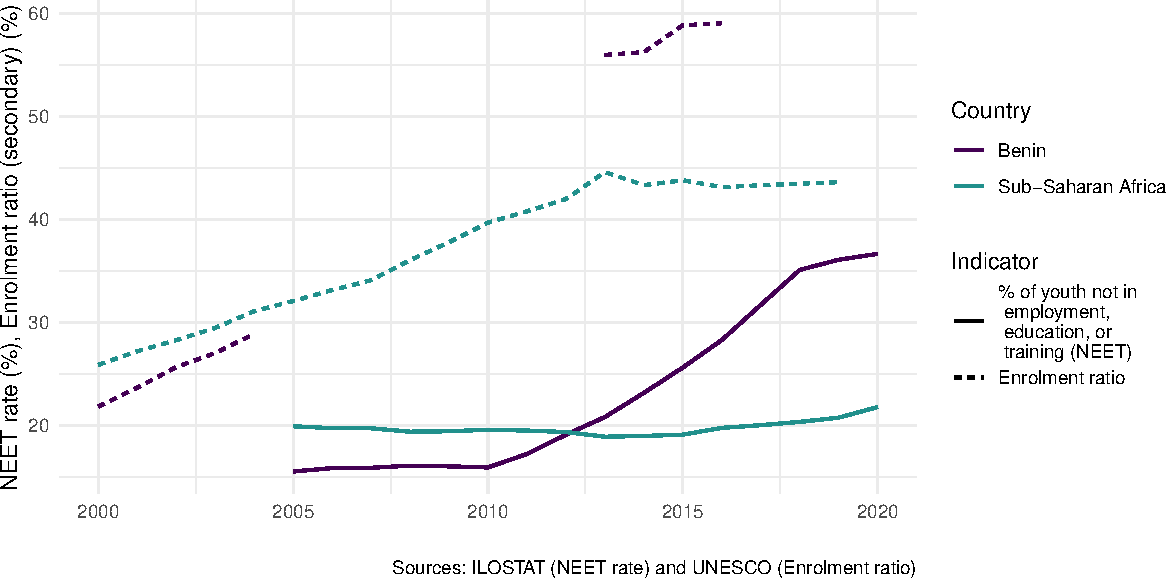
\includegraphics{figures/fig-enrollment-1} \caption{Rates of youth enrollment and inactivity: Bénin and SSA}\label{fig:fig-enrollment}
\end{figure}

\hlc[lightgray]{Despite the relative stability of its democratic government and strategic importance as a transportation hub for West Africa, Bénin (population approx. 12.1 million) performs poorly on many development indicators, ranking 158th out of 189 countries on the 2020 Human Development Index. Youth employment is a particularly pressing issue, with youth labor force participation decreasing from 53.9 percent in 2003 to 32.8 in 2018, according to the Enquête Modulaire et Intégrée sur les Conditions de Vie des Ménages (EMICOV).}\footnote{The youth labor force participation rate is defined as the number of youth age 15 to 24 as a percent of the population in the same age range.}\hlc[lightgray]{ As in other parts of SSA, secondary and tertiary school enrollment has seen a steady increase in the past two decades, coinciding with a sharp decrease in the youth employment rate: according to the most recent labor force surveys, the youth employment-to-population ratio decreased by 20 percent, from 40 to 31.5 percent, between 2010 and 2018, compared to an 13 percent decrease for adults age 25 or older over the same time period.}\footnote{The employment-to-population ratio is the proportion of a country's population in a given age range that is employed. Youth are defined to be aged 15-24.}\hlc[lightgray]{ Meanwhile, the share of youth neither in employment, education or training (NEET) increased from 17 percent in 2011 to 35 percent in 2018 (see Figure }\ref{fig:fig-enrollment}\hlc[lightgray]{) --- one the highest rates in West Africa, and the world }\autocite{ilo2022}.

\hlc[lightgray]{As enrollment in formal education has not translated to increasing rates of youth employment, interest in promoting alternative pathways to the labor force has grown. In Bénin, entry into formal technical and vocational education and training (TVET) begins after the completion of the second year of secondary school, or nine years of education. Yet across the country, the median number of years spent in the education system is just four; only five percent of youth of secondary school age are enrolled in TVET }\autocite{ilo2021}\hlc[lightgray]{, in line with the six percent of young workers estimated to participate in formal TVET across SSA }\autocite{hofmann2022}\hlc[lightgray]{. Thus, rather than formal TVET, it is informal apprenticeship that is the primary conduit into the labor market for early school leavers in Bénin, with as many as 300,000 young men and women estimated to be in training} \autocite{ilo2021}\hlc[lightgray]{. Recent examples of investment in Bénin's apprenticeship system include \$6.3 million from the World Bank for the Benin Youth Employment Project (PEJ), completed in 2019, and a planned \$16.4 million dollar investment in strengthening the TVET system starting in 2020 }\autocite{worldbank2020a}.

\hlc[lightgray]{In 2005, the government of Bénin announced a restructuring of informal apprenticeship in the informal sector. Two national apprenticeship schemes were introduced: a formalization of informal, firm-based apprenticeship called the \textit{Certificat de Qualification aux Métiers}, which introduced a national certificate for the completion of traditional training, and the dual system \textit{Certificat de Qualification Professionnelle} (CQP) program, which sought to combine in-firm, firm-specific training with more general classroom-based teaching, and to accredit the training though a separate nationally-recognized certificate. The three stated objectives of the CQP reform were to (i) offer practical and theoretical training to youth under apprenticeship contracts in the craft sector (ii) train a high-performance labor force; and (iii) improve the productivity and profitability of workshops in the craft sector }\autocite{davodoun2011}.

\hlc[lightgray]{The CQP is currently available for 13 out of the more than 300 trades listed in the craft sector: auto mechanics, motorcycle mechanics, air conditioning installers, tailors, masons, carpenters, metalworkers (primarily welding of gates for living compounds), electricians, and plumbers.}\footnote{This selection of trades was based at least in part on existing trades from early experimental dual training programs to take advantage of existing training center infrastructure. The CQM is available for about 50 trades.} \hlc[lightgray]{To participate in the CQP, applicants must (i) be at least 14 years old, unless otherwise authorized by the labor inspector; (ii) have a written apprenticeship contract that complies with labor laws; (iii) have completed at least 6 years of formal schooling; (iv) pass a national entry examination; and (v) receive funding from the Fonds de Développement de la Formation Professionnelle Continue et de l’Apprentissage (FODEFCA), the government body responsible for procuring and distributing funding for the program }\autocite{kofswisseconomicinstitute2017}\hlc[lightgray]{. Firm owners apply on behalf of the apprentices already in their charge, generally through local craftsmen associations. After three to four years of training, CQP apprentices may attempt the final examination, which takes place on one date a year for the entire nation, has a practical and a written component, and is overseen by state representatives and local craftsmen. Upon successful completion of this exam, apprentices receive a nationally-recognized certificate.}

\hlc[lightgray]{The main government organs tasked with the administration of the CQP are the national TVET directorate (DETFP), which is in charge of apprentice recruitment and training center accreditation, the Direction of Test and Exam Services (DEC), in charge of the entrance and exit examinations, and FODEFCA }\autocite{nouatin2019}\hlc[lightgray]{. The CQP began curriculum planning in 2005 with technical assistance from the French Development Agency (AFD) and the Swiss Agency for Development and Cooperation (SDC), among others, and became operational in 2008. In 2012, management of the program passed from Swisscontact, a Swiss NGO, entirely into the hands of FODEFCA }\autocite{nouatin2019}\hlc[lightgray]{. Cost sharing for the CQP program is shared by the state and the apprentice, with the state financing body for dual apprenticeship, FODEFCA, officially taking on 90 percent of the training costs }\autocite{kofswisseconomicinstitute2017}\hlc[lightgray]{. However, FODEFCA is largely reliant on external donor funding, and regular financing has been an issue for the program in recent years} \autocite{david-gnahoui2017}. \hlc[lightgray]{The financing of dual training comprises three main budget items: the costs of training to the firm, the administration of the vocational training center, and expenses for entry tests, the final examination, and certification. While on-the-job training in the firm is paid for by the apprentice or their parents, activities in the vocational training centers are largely financed through FODEFCA from various sources (national budget, donors, NGOs, etc.). Certification upon successful completion of the CQP is allocated to the national budget via the Directorate of Examinations, DEC }\autocite{david-gnahoui2017}.

\hypertarget{data}{%
\section{Data and Methods}\label{data}}

\hypertarget{sampling-and-attrition}{%
\subsection{Sampling and Attrition}\label{sampling-and-attrition}}

The data for this study was collected in two interlinked surveys. The first consisted of interviews with apprentices who had applied to the 2019 cohort of the CQP program, who took the entrance exam on the 5th of November, 2018. The second survey was conducted with the firm owners, or master craftsmen, of the apprentices' respective training firms. To allow for trade-level controls and to reduce travel distances for interviews, apprentices were randomly selected from a subsample of all CQP applicants: those training in electrical installation, carpentry, masonry, metalwork or plumbing workshops, and training in the southernmost regions of Bénin.

In addition to questions regarding training practices and firm performance, master craftsmen were asked to assess specific apprentices training at their firm. Up to two CQP applicants per firm\footnote{Only CQP applicants who had participated in the apprentice survey could be assessed individually by MCs.} were selected for this exercise. In addition, a single apprentice who had not applied to the CQP was assessed by the craftsman in a similar manner, if there was such an apprentice training in the firm.\footnote{As the apprentice survey consisted only of applicants to the program, the only data on non-applicants comes from master craftsmen.} The sampling procedure for choosing the apprentices for these personal assessments is summarized in Table \ref{tab:sampling} above.

\singlespacing

\begin{longtable}[]{@{}
  >{\raggedright\arraybackslash}p{(\columnwidth - 6\tabcolsep) * \real{0.2500}}
  >{\raggedright\arraybackslash}p{(\columnwidth - 6\tabcolsep) * \real{0.2500}}
  >{\raggedright\arraybackslash}p{(\columnwidth - 6\tabcolsep) * \real{0.2500}}
  >{\raggedright\arraybackslash}p{(\columnwidth - 6\tabcolsep) * \real{0.2500}}@{}}
\caption{\label{tab:sampling} Apprentice Sampling}\tabularnewline
\toprule\noalign{}
\begin{minipage}[b]{\linewidth}\raggedright
CQP Status
\end{minipage} & \begin{minipage}[b]{\linewidth}\raggedright
Explanation
\end{minipage} & \begin{minipage}[b]{\linewidth}\raggedright
Apprentice Survey
\end{minipage} & \begin{minipage}[b]{\linewidth}\raggedright
Firm Survey
\end{minipage} \\
\midrule\noalign{}
\endfirsthead
\toprule\noalign{}
\begin{minipage}[b]{\linewidth}\raggedright
CQP Status
\end{minipage} & \begin{minipage}[b]{\linewidth}\raggedright
Explanation
\end{minipage} & \begin{minipage}[b]{\linewidth}\raggedright
Apprentice Survey
\end{minipage} & \begin{minipage}[b]{\linewidth}\raggedright
Firm Survey
\end{minipage} \\
\midrule\noalign{}
\endhead
\bottomrule\noalign{}
\endlastfoot
\textbf{Selected} into CQP & Applied to CQP in 2019 through master craftsmen. Passed exam and was admitted to program. & Random sampling from list of all CQP applicants in five chosen trades and from southern Bénin) & Master craftsman assesses \emph{at most} two apprentices, randomly chosen from all CQP selected/not selected in firm at baseline. \\
& & & \\
CQP applicant but \textbf{Not Selected} & Applied to CQP in 2019 through master craftsmen. Was not admitted due to exam score or lack of proximate training center. & Random sampling from list of all CQP applicants in five chosen trades and from southern Bénin) & Master craftsman assesses \emph{at most} two apprentices, randomly chosen from all CQP selected/not selected in firm at baseline. \\
& & & \\
\textbf{Did Not Apply} to CQP & Did not apply to CQP. Training as traditional apprentice. & N/A & Master craftsman lists \emph{up to} 5 apprentices who did not apply to CQP. Assesses only one, randomly chosen at baseline. \\
\end{longtable}

\onehalfspacing

The baseline wave for the two surveys was collected in July-August 2019. The apprentice survey included questions on training characteristics, employment outcomes, their own skills and competences, and the perceived quality of their training, while the firm survey included questions on worker characteristics, wages, and firm expenses and revenues. We additionally surveyed all MCs about the firm's training practices and expenses, as well as their perception of up to three individual apprentices' skills, experience, diligence, efficiency, learning ability, and so on (sampling procedure detailed above). Data on 427 apprentices working for 197 unique firms was collected at baseline. Descriptive statistics for apprentices and firms are shown in Table \ref{tab:tbl-cqpdesc} below.

\begin{singlespacing}
\begin{table}[H]

\caption{\label{tab:tbl-cqpdesc}Descriptive Statistics}
\centering
\resizebox{\linewidth}{!}{
\begin{threeparttable}
\begin{tabular}[t]{lcccccc}
\toprule
\multicolumn{1}{c}{ } & \multicolumn{2}{c}{Overall} & \multicolumn{4}{c}{By baseline status} \\
\cmidrule(l{3pt}r{3pt}){2-3} \cmidrule(l{3pt}r{3pt}){4-7}
\textbf{Characteristic} & \textbf{Baseline} & \textbf{Endline} & \textbf{Selected} & \textbf{Not Selected} & \textbf{Did Not Apply} & \textbf{p-value}\\
\midrule
\addlinespace[0.3em]
\multicolumn{7}{l}{\textbf{Apprentices}}\\
\hspace{1em}N & 427 & 240 & 149 & 107 & 171 & \\
\hspace{1em}Age & 21.3 (3.4) & 23.2 (3.5) & 21.7 (2.8) & 22.3 (4.1) & 20.1 (3.2) & <0.001\\
\hspace{1em}Male & 98\% & 98\% & 99\% & 98\% & 97\% & >0.9\\
\hspace{1em}Trade &  &  &  &  &  & <0.001\\
\hspace{1em}\hspace{1em}Masonry & 21\% & 18\% & 19\% & 23\% & 22\% & \\
\hspace{1em}\hspace{1em}Carpentry & 11\% & 11\% & 13\% & 6.5\% & 12\% & \\
\hspace{1em}\hspace{1em}Plumbing & 13\% & 15\% & 17\% & 11\% & 9.4\% & \\
\hspace{1em}\hspace{1em}Metalworking & 20\% & 20\% & 28\% & 12\% & 19\% & \\
\hspace{1em}\hspace{1em}Electrical Inst. & 35\% & 36\% & 22\% & 47\% & 38\% & \\
\hspace{1em}Years in training & 2.33 (1.38) & 4.39 (1.38) & 2.52 (1.24) & 2.64 (1.30) & 1.92 (1.48) & <0.001\\
\hspace{1em}Education &  &  &  &  &  & \\
\hspace{1em}\hspace{1em}None & 2.5\% & 3.3\% & 0\% & 0.9\% & 6.0\% & \\
\hspace{1em}\hspace{1em}<Primary & 15\% & 15\% & 6.0\% & 6.5\% & 30\% & \\
\hspace{1em}\hspace{1em}Primary & 22\% & 21\% & 21\% & 32\% & 17\% & \\
\hspace{1em}\hspace{1em}Secondary & 57\% & 57\% & 66\% & 59\% & 45\% & \\
\hspace{1em}\hspace{1em}Technical & 2.0\% & 2.5\% & 2.7\% & 0.9\% & 2.0\% & \\
\hspace{1em}\hspace{1em}Tertiary & 1.5\% & 1.3\% & 3.4\% & 0.9\% & 0\% & \\
\hspace{1em}Status at endline &  &  &  &  &  & <0.001\\
\hspace{1em}\hspace{1em}Still training & - & 73\% & 92\% & 69\% & 55\% & \\
\hspace{1em}\hspace{1em}Graduated & - & 17\% & 6.7\% & 29\% & 21\% & \\
\hspace{1em}\hspace{1em}Dropped out & - & 2.5\% & 1.1\% & 1.7\% & 3.6\% & \\
\hspace{1em}\hspace{1em}Unknown & - & 7.1\% & 0\% & 0\% & 20\% & \\
\addlinespace[0.3em]
\hline
\multicolumn{7}{l}{\textbf{Firms}}\\
\hspace{1em}N & 197 & 150 &  &  &  & \\
\addlinespace[0.3em]
\multicolumn{7}{l}{\hspace{1em}Apprentices trained}\\
\hspace{1em}\hspace{1em}Total & 5.4 (4.7) & 5.5 (6.0) &  &  &  & \\
\hspace{1em}\hspace{1em}Selected & 1.20 (1.82) & 1.10 (1.55) &  &  &  & \\
\hspace{1em}\hspace{1em}Not Selected & 1.47 (2.68) & 1.41 (2.86) &  &  &  & \\
\hspace{1em}\hspace{1em}Did Not Apply & 2.7 (3.1) & 2.8 (3.1) &  &  &  & \\
\addlinespace[0.3em]
\multicolumn{7}{l}{\hspace{1em}Firm size}\\
\hspace{1em}\hspace{1em}Total (calculated)¹ & 8.8 (9.1) & 8.2 (8.6) &  &  &  & \\
\hspace{1em}\hspace{1em}Total (reported) & 6.7 (7.5) & 6.6 (7.1) &  &  &  & \\
\hspace{1em}\hspace{1em}Apprentices & 5.4 (4.7) & 5.5 (6.0) &  &  &  & \\
\hspace{1em}\hspace{1em}Permanent wage & 0.36 (1.8) & 0.80 (2.8) &  &  &  & \\
\hspace{1em}\hspace{1em}Paid family & 0.06 (0.4) & 0.14 (0.6) &  &  &  & \\
\hspace{1em}\hspace{1em}Unpaid family & 0.05 (0.4) & 0.03 (0.2) &  &  &  & \\
\hspace{1em}\hspace{1em}Occasional & 0.83 (2.6) & 0.83 (2.3) &  &  &  & \\
\hspace{1em}Trade &  &  &  &  &  & \\
\hspace{1em}\hspace{1em}Masonry & 23\% & 20\% &  &  &  & \\
\hspace{1em}\hspace{1em}Carpentry & 12\% & 12\% &  &  &  & \\
\hspace{1em}\hspace{1em}Plumbing & 13\% & 14\% &  &  &  & \\
\hspace{1em}\hspace{1em}Metalworking & 20\% & 21\% &  &  &  & \\
\hspace{1em}\hspace{1em}Electrical Inst. & 32\% & 33\% &  &  &  & \\
\bottomrule
\end{tabular}
\begin{tablenotes}
\small
\item \textit{Notes:} N; Mean (SD); %
\item[1] Calculated by author by summing number of partners, permanent employees, paid and unpaid family workers, occasional workers, and apprentices reported to be working for MC (total firm size reported separately).
\end{tablenotes}
\end{threeparttable}}
\end{table}
\end{singlespacing}

Summary statistics from the baseline survey show the sample to be predominantly male youth who, though of average age for an apprenticeship at 21.3 years \autocite{ilo2022}, are significantly more educated than is typical for traditional apprentices, with over half having completed at least some secondary schooling. Successful applicants to the CQP have higher education attainment than unsuccessful applicants; all applicants have higher attainment than non-applicants. Applicants also have more experience coming into the CQP than the required six months, with the average applicant having trained for 1.9 years at the time of application. Non-applicants are younger, less educated, and less experienced than applicants at baseline, suggesting that master craftsmen send their most able and veteran apprentices to stand for the dual training entrance exam. This may indicate that the CQP is perceived by MCs as something more akin to a continuing education rather than an entry-level apprenticeship program.

The majority of training firms are small workshops comprising the firm owner --- the master trainer --- and several apprentices. Two firm sizes are shown in Table \ref{tab:tbl-cqpdesc}: those stated directly by the firm owner in response to the question, ``How many people (including you and your apprentices) are currently working in your business?'' and those calculated by the author by summing the number of apprentices, partners, paid and unpaid family workers, and occasional workers reportedly participating in firm activities. Using self-reported size, 94.8 percent of firms employed a total of five people or less (including the owner) at baseline and 96.8 percent employed no more than ten (97.1 and 99.5 percent, respectively, using author-calculated size).Thus, training firms in the sample are small, in line with observations from the informal sector in Ghana \autocite{frazer2006,velenchik1995}, but also roughly similar to the size distribution of a sample of Swiss firms reported by \textcite{muhlemann2007}-\footnote{Our sample has a higher density of firms with three to nine employees, whereas the Swiss sample (which includes non-training firms) has a higher density of firms with three total employees or fewer. This shift can be explained by the large number of apprentices in the Béninese training firm sample: at baseline, the average firm employed about four apprentices for every other type of employee, or a total of six apprentices.}

\todo{16}\hlc[pink]{The endline survey was conducted in August-September 2021. Overall apprentice attrition in our sample, at 43.8 percent, is clearly very high, even when compared to studies in similar contexts: for instance, }\textcite{crepon2019}\} \hlc[pink]{and }\textcite{hardy2019}\hlc[pink]{ both report youth attrition of around 10 percent, though it is generally common for studies of training programs to be affected by high rates of attrition }\autocite{mckenzie2017}. \hlc[pink]{Both youth non-response and firm non-response}\footnote{Data on apprentices who had not applied to the CQP was only obtained from firm owners, and is thus only subject to firm attrition.} \hlc[pink]{drive attrition in our sample. We assess the severity of this problem by testing for differences between retained and attritted apprentices in terms of relevant baseline characteristics such as CQP participation, trade, or socioeconomic variables. Tables} \ref{tab:tbl-attritionapps}\hlc[pink]{ in the Appendix gives no indication of such differences. In Table }\ref{tab:tbl-attritionappsreg}\hlc[pink]{, also in the Appendix, we estimate a logit model where attrition is a function of CQP status at baseline and other apprentice characteristics; again, we find no systematic bias. At only 1 percent, reported program dropout among CQP participants retained in the sample is very low compared to similar studies, e.g. }\textcite{crepon2019}\hlc[pink]{ who report 31.2 percent dropout for dual apprenticeships and 32.5 percent for informal apprenticeships. Sample attrition may be correlated with program dropout, but we are unable to test for this possibility with the available data. Finally, despite starting with comparable experience at baseline, unsuccessful applicants to the CQP are more likely to have graduated after three years than CQP participants --- Covid-19 related interruptions to training and the single annual CQP examination date both likely contributed to the low graduation rate of CQP apprentices after three years.}

\hlc[pink]{Similarly, of 197 firms interviewed at baseline, only 150 could be contacted at endline, for an overall firm attrition rate of 23.9 percent. Tables }\ref{tab:tbl-attritionfirms}\hlc[pink]{ and }\ref{tab:tbl-attritionfirmsreg}\hlc[pink]{ in Appendix A4 likewise suggest that firm attrition was not correlated with key firm characteristics such as size or profitability, though a logit model of attrition shows that firms with a higher proportion of CQP participants among their apprentices are somewhat more likely to exit the sample.}

\todo{18}\hl{Although tests revealed no statistically significant attrition bias based on trade or socio-economic factors, potential reasons for non-response remain. Although Fon and French was spoken by the enumerators, surveys were not conducted in local languages spoken by the apprentices or craftsmen, and some individuals might not have been able to participate due to difficulty understanding the questions. Though the remote follow-up surveys were significantly shorter than the baseline and endline surveys, participants may have dropped out due to time constraints: apprentices and craftsmen may have been too busy with work or personal commitments to dedicate time to completing the surveys. Changing phone numbers is a common practice in Bénin, and though contacts such as friends and family members were elicited for the case that a participant had changed numbers between waves, it is possible that the difficulty of tracking down youth who had changed numbers was simply insurmountable in individual cases. Finally, privacy is highly valued in Bénin, and certain participants looked at our data collection with suspicion. It is possible that security and privacy concerned also caused a number of apprentices and trainers to drop out from the survey.}

\hypertarget{appmethod}{%
\subsection{Estimating Apprentice Benefits}\label{appmethod}}

We first examine the benefits accruing to apprentices over the observed time period of three years. These benefits can be separated into two categories: human capital gains and material benefits.

Human capital gains are measured using a set of trade-specific scores measured separately for each apprentice at baseline and endline. These amount to a simplified version of the ``task approach'' utilized in the technological change literature \autocites[see][]{dicarlo2016,crepon2019}. Unlike the general tasks used to measure skills in the task approach, however, we measure apprentice knowledge by means of a short test based on CQP curricula. Each question was a multiple choice question, and between 4 and 5 knowledge questions were posed to each apprentice; because apprentices who did not apply to the CQP were not interviewed directly, the knowledge score was only measured for CQP applicants. The questions are reproduced in Appendix B4.

Our measures of competence and experience, on the other hand, are based on a short roster of tasks drafted in collaboration with local craft experts and practitioners, an approach similar to that employed by \textcite{hardy2019} (all tasks are shown in Appendix B4). Firms were asked to assess apprentices on this series of 10 to 15 trade-relevant tasks,\footnote{Apprentices were asked to self-evaluate their competence at endline using the same metric. Self-evaluation was not initially planned and thus unavailable at baseline.} and the percentage of tasks in which apprentices are deemed competent or experienced (on a binary scale) constitute their score in each of the two measures. Similar to the task approach, this method allows for worker-level measurement of ability and experience based on tasks performed. Each apprentice received a score in each of the three dimensions.

Regression analysis is then used to examine the impact of dual training on these three measures of apprentice learning. We use the specification

\[ y_{it} = a+\sum_{j}\text{status}_{ij}+\sum_{k}\text{status}_{ik}\text{×}Endline_t+{Endline}_t+\mathbf{X}_{it}+\mathbf{Z}_{jt}+u_{it} \]
where \(y_{it}\) is the outcome for apprentice \(i\) at time \(t\), \(\text{status}_{ij}\) corresponds to apprentice status \(j\) of apprentice \(i\) in the context of the CQP program: either successful applicant, unsuccessful applicant, or non-applicant, and \(\sum_{k}\text{status}_{ik}\text{×}Endline_t+{Endline}_t\) are the interaction of a CQP participation dummy and survey wave and a dummy for CQP non-applicants and survey wave. These interactions identify any gains in learning outcomes that can be linked to CQP participation. \(\mathbf{X}_{it}\) is a column vector of apprentice characteristics, \(\mathbf{Z}_{jt}\) is a column vector of training-related firm characteristics, \(a\) is a constant, and \(u_{it}\) is an error term.

Finally, we assess the material benefits of training accruing to the apprentice, calculated simply as total fees paid less allowances received. These two categories of transactions between MC and apprentices are described in greater detail in the next section.

\hypertarget{firmmethod}{%
\subsection{Estimating Firm Benefits}\label{firmmethod}}

\begin{singlespacing}
\begin{table}[H]
\caption{Components of net benefit accounting}
\label{tab:tbl-cbmodels}
\setlength{\tabcolsep}{8pt}
\renewcommand{\arraystretch}{1.25}
\resizebox{\textwidth}{!}{%
  \begin{tabular}{llllllll}
  \multicolumn{3}{l|}{}                                                              & \multicolumn{5}{c}{\textbf{Model}}                                 \\
  & \textbf{Estimate} & \multicolumn{1}{l|}{\textbf{Assumptions}}        & \textbf{I} & \textbf{II} & \textbf{III} & \textbf{IV} & \textbf{V} \\ \hline
  \multicolumn{8}{l}{\textbf{Benefits}}                                                                                                                   \\ \hline
  Annual fees & Total fees / 4    & \multicolumn{1}{l|}{Four year training duration} & \textbf{\times} & \textbf{\times}  & \textbf{\times}   & \textbf{\times}  & \textbf{\times} \\ \hline
  \begin{tabular}[c]{@{}l@{}}Annual\\ apprentice\\ productivity\end{tabular} &
    \begin{tabular}[c]{@{}l@{}}Average of monthly wages\\ of experienced and \\ inexperienced employee \times \\ \# of months/year operational\end{tabular} &
  \multicolumn{1}{l|}{\begin{tabular}[c]{@{}l@{}}Wages equal to productivity.\\ Apprentice prod. equal to \\ that of untrained employees \\ for first two years and trained \\ employee for final two years\end{tabular}} &
    \textbf{} &
    \textbf{} &
    \textbf{\times} &
    \textbf{\times} &
    \textbf{\times} \\ \hline
  \multicolumn{8}{l}{\textbf{Costs}}                                                                                                                      \\ \hline
  \begin{tabular}[c]{@{}l@{}}Annual\\ allowances\end{tabular} &
    \begin{tabular}[c]{@{}l@{}}Daily allowances \times \, 20 days \times\\ \# of months/year operational\end{tabular} &
  \multicolumn{1}{l|}{\begin{tabular}[c]{@{}l@{}}Apprentices work 20\\ days/month\end{tabular}} &
    \textbf{\times} &
    \textbf{\times} &
    \textbf{\times} &
    \textbf{\times} &
    \textbf{\times} \\ \hline
  \begin{tabular}[c]{@{}l@{}}Annual\\ training\\ expenses\end{tabular} &
    \begin{tabular}[c]{@{}l@{}}Total monthly training \\ expenses / \# of apprentices \times\\ \# of months/year operational\end{tabular} &
  \multicolumn{1}{l|}{\begin{tabular}[c]{@{}l@{}}All reported training\\ expenses are recurring\end{tabular}} &
    \textbf{} &
    \textbf{\times} &
    \textbf{} &
    \textbf{\times} &
    \textbf{\times} \\ \hline
  \begin{tabular}[c]{@{}l@{}}Annual lost\\ trainer\\ productivity\end{tabular} &
    \begin{tabular}[c]{@{}l@{}}Monthly wages of experienced\\ employee \times \, estimated hours of\\ training per month \times\\ \# of trainers/apprentice \times \\ \# of months/year operational\end{tabular} &
  \multicolumn{1}{l|}{\begin{tabular}[c]{@{}l@{}}Wages equal to productivity.\\ All trainers in firm stop\\ working simultaneously\\ when firm pauses activities \\ to train apprentices.\end{tabular}} &
    &
    &
    &
    &
    \textbf{\times}
  \end{tabular}%
}
\end{table}
\end{singlespacing}

\todo{18} \hl{We employ an accounting approach }\autocite{gambin2013,muhlemann2014}\hl{ to estimate the net benefits accruing to firms from training apprentices. This method involves calculating and summing the various cost and benefit components associated with training provision, and} \hlc[lightgray]{has only recently started being applied in lower-middle income countries }\autocite{renold2018,bolli2020,bolli2021}. \hl{Specifically, we construct five progressively complex models to estimate net benefits accruing to firms from their apprentice-training activities. Each model consists of a combination of the following benefits and costs which are estimated from the apprentice and benefit survey data.}

\hl{\textbf{Benefits}: Two primary benefits are considered. First, apprenticeship fees encompass various payments made by apprentices or their families throughout the training program. These fees are categorized and reported by both apprentices and master craftsmen, ensuring comprehensive accounting. Second, the productive contributions of apprentices are estimated using the assumption of a competitive labor market. Based on wage data and training duration, the study approximates apprentice productivity over the four-year program, contributing to the overall value generated for the firm.}

\hl{\textbf{Costs}: Three main cost categories are incorporated. Allowances, representing irregular expenditures for apprentice needs like travel and meals, are estimated by summing reported allowance categories and extrapolating to annual figures. Training expenses, encompassing costs for equipment, materials, rent, and training materials, are reported by training firms. These firm-level costs are then divided by the number of apprentices and annualized to accurately reflect the per-apprentice, per-year expenditure. Finally, lost trainer productivity is estimated by multiplying reported work hours lost due to training activities by hourly wages.}

\hl{\textbf{Cost-Benefit Models}: By summing these calculated cost and benefit components, we arrive at an estimate of the net benefit generated by training apprentices for the firm. The models gradually incorporate additional components, increasing both the comprehensiveness and the number of assumptions underlying the net benefit model (Table }\ref{tab:tbl-cbmodels}). \textbf{Model I}, \hl{representing the simplest approach, focuses solely on direct financial flows. It subtracts reported training costs from the total apprenticeship fees received by the firm. }\textbf{Model II} \hl{introduces the first layer of assumptions by incorporating estimated apprentice productivity based on wage data and training duration. Building upon this, }\textbf{Model III} \hl{adds training expenses, encompassing documented costs for equipment, materials, and training facilities, to provide a more comprehensive picture of firm expenditures. }\textbf{Model IV}\hl{ combines features of Models II and III, accounting for both estimated apprentice contributions and training expenses. Finally, }\textbf{Model V} \hl{incorporates all cost and benefit components, including the most assumption-laden estimate, namely lost trainer productivity due to training activities. This stepwise approach allows us to gradually increase the complexity and number of underlying assumptions on the calculation of firm net benefits, such that a balance between the completeness and reliability of the model can be found.}

\hypertarget{section-3}{%
\subsubsection*{\texorpdfstring{\hl{Benefits in detail}}{}}\label{section-3}}

\todo{18,19}

\hlc[lightgray]{Firms receive two primary benefits from training: apprenticeship fees and the apprentices' productive contributions to the firm. Training fees can be paid in full before the commencement of training or split into payment at the beginning, during, and at the conclusion of training }\autocite{velenchik1995}\hlc[lightgray]{. Six categories of fees were reported by both apprentices and MCs: entry fees, formation (or general training) fees, liberation (or graduation) fees paid at the conclusion of training, fees as compensation for the materials and equipment used in training, contract fees, and application fees.}\footnote{Fees are often paid in kind rather than in cash.} \hlc[lightgray]{Fees were reported as the total paid for the entirety of the apprenticeship; we assume four-year apprenticeships to estimate annual amounts.}

\hlc[lightgray]{The second benefit of training for firms -- apprentices' net productive contributions -- were not reported explicitly by the firm owners and thus needed to be estimated on the basis of several assumptions. First, we assume the competitive model of labor markets (with heterogeneous wages), in which workers are paid the marginal product of their labor. Second, we assume apprentice productivity is equal to that of an untrained employee with no more than a primary education for the first two years of training, and increases to that of trained employee for the final two years,}\footnote{This is a simplification of the approach used by Bolli, Bolli-Kemper, et al. (2020), in which apprentice productivity is estimated to increase linearly from that of an unskilled worker to that of a skilled worker between defined points in their training. A popular alternative to this approach involves eliciting specific tasks performed by apprentices and estimating costs savings based on the wages paid to workers who would otherwise be responsible for said tasks (Hauschildt 2018). Our firm-apprentice data did not cover specific tasks and is thus not equipped to carry out such an analysis.} \hlc[lightgray]{and we use detailed wage information reported by firm owners to estimate the average annual productivity over the course of a four-year apprenticeship. Under these assumptions, the annual productive value generated by apprentice work amounts to the average of these two wages.}

\hypertarget{section-4}{%
\subsubsection*{\texorpdfstring{\hl{Costs in Detail}}{}}\label{section-4}}

\todo{18,19}

\hlc[lightgray]{Costs of apprenticeship for the firm are categorized into three categories: allowances, training expenses, and lost trainer productivity.}

\hlc[lightgray]{Allowances are disbursed irregularly by the firm owner for small expenses such as travel and meals. These are reported by firms at the apprentice level (separate reported allowances for each apprentice). To estimate total annual allowance expenditures per apprentice, we thus sum over all allowance categories and assume that apprentices work 20 days per month; the extrapolated monthly sum is then multiplied by the number of months the training firm was operating in the past year to arrive at an annual estimate for each apprentice. Alternative estimates using different workload assumptions or substituting firm-reported with apprentice-reported figures are shown in Table }\ref{tab:tbl-allowancebounds} and Table \ref{tab:tbl-allowboundsapp}\hlc[lightgray]{ in Appendix A4.}

\hlc[lightgray]{To help estimate the training costs paid by the firm, owners were asked to identify any costs directly or indirectly related to their training activities. Specific training costs include equipment costs, which comprise all costs for physical infrastructure necessary for training; raw materials such as cement, lumber, or scrap metal used for demonstration or practice purposes; training equipment such as workbenches, toolkits, or other machines purchased or rented specifically for apprentices; rent for training facilities if training was not conducted exclusively in the MC's workshop; and books and any other training materials. Firms reported the training costs in each category for the month prior to the interview; to estimate annual training costs per apprentice per year, the reported firm-level costs are divided by the number of apprentices training in the firm and multiplied by the number of months the firm was open in the previous year.}

\hlc[lightgray]{An additional cost paid by the training firm comes in the form of time lost by training staff when they would have otherwise been engaged in productive activities. Lost trainer productivity is, like apprentice productivity, estimated using wage data. Hourly wages for skilled employees were calculated from monthly wage data and multiplied by the number of hours that the workshop stopped all productive activities to train apprentices in the previous week, as reported by the MC. This estimate is burdened by the largest number of assumptions: it is uncertain whether all employees who train apprentices in the firm (a number reported by the MC) stop work entirely while the workshop interrupts normal productive activities to train; whether the majority of lost productivity occurs during these breaks, or in the otherwise normal operation of the firm during which they must also tend to the apprentices. Moreover, the total duration of these breaks in the past week is a very small sample from which to extrapolate to annual costs. Lacking a better method, we report these estimates as the final cost component.}

\hypertarget{regression-analysis}{%
\subsubsection*{Regression Analysis}\label{regression-analysis}}

In a final step, we study the effect of hiring apprentices, both traditional and those participating in the CQP, on firm size and profits by estimating the following regression:

\[ y_{it} =  a+CQP_i+{Endline}_t+apprentices_{it}+\mathbf{X}_{it}+u_{it}, \]

where \(y_{it}\) is the outcome of interest, \(CQP_i\) is the number of CQP applicants who were accepted into the 2019 cohort of the program. \(apprentices_{it}\) controls for the total number of apprentices training with the firm and not participating in the CQP program (and in contrast to \(CQP_i\) is a time-varying measure), while \(\mathbf{X}_{it}\) is a matrix of additional covariates for firm \(i\) in wave \(t\), \({Endline}_t\) is a dummy variable denoting survey wave, \(a\) is a constant, and \(u_{it}\) is an error term.

\hypertarget{cqpresults}{%
\section{Results}\label{cqpresults}}

\hypertarget{appbenefits}{%
\subsection{Impact of Informal and Dual Training on Individuals}\label{appbenefits}}

First, we investigate whether dual training was successful in realizing its primary objective --- increasing the human capital stock of apprentices. To do so, we study the changes in the three human capital indices described in Section \ref{appmethod} over the observed training period of three years.

\begin{singlespacing}
\begin{table}[H]

\caption{\label{tab:tbl-skills}Change in apprentice human capital}
\centering
\fontsize{10}{12}\selectfont
\resizebox{\linewidth}{!}{
\begin{threeparttable}
\begin{tabular}[t]{lcccccc}
\toprule
 & \textbf{N} & \textbf{Baseline} & \textbf{N} & \textbf{Endline} & \textbf{Difference} & \textbf{p-value³}\\
\midrule
\addlinespace[0.3em]
\multicolumn{7}{l}{\textbf{Competence¹}}\\
\hspace{1em}Electrical Installation & 125 & 0.80 (0.24) & 69 & 0.96 (0.09) & 0.09 & <0.001\\
\hspace{1em}Masonry & 90 & 0.75 (0.22) & 39 & 0.90 (0.18) & 0.14 & 0.008\\
\hspace{1em}Carpentry & 48 & 0.76 (0.28) & 21 & 0.93 (0.15) & 0.12 & 0.14\\
\hspace{1em}Plumbing & 54 & 0.73 (0.29) & 26 & 0.92 (0.15) & 0.15 & 0.008\\
\hspace{1em}Metalwork & 86 & 0.75 (0.22) & 38 & 0.86 (0.21) & 0.09 & 0.006\\
\hspace{1em}CQP Selected & 143 & 0.81 (0.21) & 82 & 0.95 (0.11) & 0.11 & <0.001\\
\hspace{1em}CQP Not Selected & 95 & 0.84 (0.19) & 56 & 0.94 (0.10) & 0.06 & 0.017\\
\hspace{1em}Did Not Apply & 165 & 0.68 (0.28) & 55 & 0.84 (0.22) & 0.16 & <0.001\\
\textbf{\hspace{1em}Overall} & \textbf{403} & \textbf{0.76 (0.24)} & \textbf{193} & \textbf{0.92 (0.16)} & \textbf{0.11} & \textbf{<0.001}\\
\addlinespace[0.3em]
\multicolumn{7}{l}{\textbf{Experience¹}}\\
\hspace{1em}Electrical Installation & 125 & 0.77 (0.26) & 69 & 0.96 (0.08) & 0.11 & <0.001\\
\hspace{1em}Masonry & 90 & 0.72 (0.23) & 39 & 0.91 (0.13) & 0.20 & <0.001\\
\hspace{1em}Carpentry & 48 & 0.73 (0.31) & 21 & 0.98 (0.06) & 0.19 & 0.013\\
\hspace{1em}Plumbing & 54 & 0.66 (0.30) & 26 & 0.89 (0.17) & 0.21 & 0.001\\
\hspace{1em}Metalwork & 86 & 0.72 (0.24) & 38 & 0.85 (0.15) & 0.13 & 0.004\\
\hspace{1em}CQP Selected & 143 & 0.78 (0.24) & 82 & 0.93 (0.11) & 0.15 & <0.001\\
\hspace{1em}CQP Not Selected & 95 & 0.80 (0.21) & 56 & 0.94 (0.11) & 0.10 & 0.001\\
\hspace{1em}Did Not Apply & 165 & 0.65 (0.29) & 55 & 0.87 (0.16) & 0.21 & <0.001\\
\textbf{\hspace{1em}Overall} & \textbf{403} & \textbf{0.73 (0.26)} & \textbf{193} & \textbf{0.92 (0.13)} & \textbf{0.15} & \textbf{<0.001}\\
\addlinespace[0.3em]
\multicolumn{7}{l}{\textbf{Knowledge²}}\\
\hspace{1em}Electrical Installation & 77 & 0.90 (0.16) & 49 & 0.93 (0.10) & 0.01 & 0.4\\
\hspace{1em}Masonry & 56 & 0.76 (0.19) & 30 & 0.83 (0.20) & 0.01 & 0.8\\
\hspace{1em}Carpentry & 25 & 0.91 (0.18) & 15 & 0.97 (0.09) & 0.05 & 0.3\\
\hspace{1em}Plumbing & 38 & 0.52 (0.12) & 26 & 0.64 (0.16) & 0.11 & 0.013\\
\hspace{1em}Metalwork & 209 & 0.85 (0.18) & 117 & 0.88 (0.15) & 0.00 & 0.8\\
\hspace{1em}CQP Selected & 144 & 0.75 (0.20) & 84 & 0.80 (0.18) & 0.03 & 0.10\\
\hspace{1em}CQP Not Selected & 103 & 0.79 (0.22) & 59 & 0.84 (0.19) & 0.02 & 0.5\\
\textbf{\hspace{1em}Overall} & \textbf{247} & \textbf{0.77 (0.21)} & \textbf{143} & \textbf{0.81 (0.19)} & \textbf{0.03} & \textbf{0.078}\\
\bottomrule
\end{tabular}
\begin{tablenotes}
\small
\item \footnotesize \textit{Notes:} Mean (SD).
\item[1] \footnotesize Percent of trade-specific tasks apprentice is deemed competent in (competence) or has already successfully attempted (experience), as reported by MC. Total of 10-15 tasks, depending on trade.
\item[2] \footnotesize Percent of trade-specific knowledge questions answered correctly by apprentice. Total of 4 or 5 questions, depending on trade. Not available for apprentices who did not apply to the CQP, as they were not interviewed personally.
\item[3] \footnotesize Paired t-test.
\end{tablenotes}
\end{threeparttable}}
\end{table}
\end{singlespacing}

The changes in the human capital index scores presented in Table \ref{tab:tbl-skills} indicate that informal apprenticeship training is successful in improving sector-specific human capital of the youth in our sample, both for dual training participants and traditional apprentices: overall competence scores increased by 0.46 SDs, experience scores by 0.58 SDs, and knowledge by 0.13 SDs. Significant improvements in competence and experience are observed for apprentices who participated in, unsuccessfully applied to, and did not apply to the CQP alike, though apprentices who did not apply to the CQP show the largest gains in competence and experience as assessed by their MC. This result is in line with the observation that MCs appear to send youth who are already relatively experienced (and educated) to apply for dual training.

A paired t-test also indicates significant improvements in competence and experience between baseline and endline across all trades (improvement in competence for plumbing apprentices is marginally insignificant at standard significance levels). On the other hand, gains in the knowledge metric are not statistically significant for any single trade except plumbing - hence, the overall increase in knowledge is driven by results from plumbing apprentices alone. As the average knowledge scores at baseline were significantly lower for plumbing apprentices than for apprentices in other trades, this result may indicate a shortcoming in the metric itself, which was composed of only up to five questions which did not seem to pose a major challenge for most apprentices in the other four trades. Improvement in knowledge was marginally significant (p \textless{} 0.10) for CQP participants but not for CQP applicants who were not selected (p \textless{} 0.5).

Although mean human capital accumulation is higher for participating CQP apprentices than non-selected CQP applicants across the three indices, this does not translate into statistically significant differences between the two group (Table \ref{tab:tbl-skillschangebycqp} in the Appendix). Nor do we observe a significant effect of dual training on the competence and experience indices when apprentices who did not apply to the CQP are added to the control group. To check if apprentices agree with their MC's assessments of their ability, a self-assessment was included in the apprentice survey at endline. Table \ref{tab:tbl-compexp2} in the Appendix suggests that the two assessments are in general agreement for both the experience and the competence index (the exception again being limited to the plumbing trade, where MCs were relatively critical in their assessment of apprentices' abilities).

\begin{singlespacing}

\begin{table}[H] \centering 
  \caption{Effects of training on human capital development} 
  \label{tab:tbl-appreg} 
\scriptsize 
\begin{tabular}{@{\extracolsep{-8pt}}lccccccccc} 
\\[-1.8ex]\hline 
\hline \\[-1.8ex] 
\\[-1.8ex] & \multicolumn{3}{c}{Experience} & \multicolumn{3}{c}{Competence} & \multicolumn{3}{c}{Knowledge} \\ 
\\[-1.8ex] & (1) & (2) & (3) & (4) & (5) & (6) & (7) & (8) & (9)\\ 
\hline \\[-1.8ex] 
 CQP Selected (reference) \\ \\ CQP Not Selected & $-$0.004 & $-$0.0002 & $-$0.02 & 0.002 & 0.01 & $-$0.002 & 0.04$^{*}$ & 0.03 & $-$0.01 \\ 
  & (0.02) & (0.03) & (0.03) & (0.02) & (0.03) & (0.03) & (0.02) & (0.03) & (0.02) \\ 
  CQP Did Not Apply & $-$0.10$^{***}$ & $-$0.12$^{***}$ & $-$0.13$^{***}$ & $-$0.11$^{***}$ & $-$0.12$^{***}$ & $-$0.13$^{***}$ &  &  &  \\ 
  & (0.02) & (0.03) & (0.03) & (0.02) & (0.02) & (0.02) &  &  &  \\ 
  Endline & 0.17$^{***}$ & 0.15$^{***}$ & 0.15$^{***}$ & 0.13$^{***}$ & 0.13$^{***}$ & 0.13$^{***}$ & 0.06$^{**}$ & 0.05$^{*}$ & 0.05$^{**}$ \\ 
  & (0.02) & (0.03) & (0.03) & (0.02) & (0.03) & (0.03) & (0.02) & (0.03) & (0.02) \\ 
  \hl{CCQP Selected x Endline (reference)} \\ \\ \hl{CCQP Not Selected x Endline} &  & $-$0.01 & $-$0.02 &  & $-$0.03 & $-$0.04 &  & 0.02 & $-$0.002 \\ 
  &  & (0.05) & (0.05) &  & (0.04) & (0.04) &  & (0.04) & (0.03) \\ 
  CQP Did Not Apply x Endline &  & 0.07 & 0.07 &  & 0.03 & 0.03 &  &  &  \\ 
  &  & (0.05) & (0.04) &  & (0.04) & (0.04) &  &  &  \\ 
  Baseline years of training$^1$ & 0.06$^{***}$ & 0.06$^{***}$ & 0.06$^{***}$ & 0.05$^{***}$ & 0.05$^{***}$ & 0.06$^{***}$ & 0.01 & 0.01 & 0.01 \\ 
  & (0.01) & (0.01) & (0.01) & (0.01) & (0.01) & (0.01) & (0.01) & (0.01) & (0.01) \\ 
  Firm Size$^2$ & $-$0.003 & $-$0.003 & $-$0.002 & $-$0.001 & $-$0.0003 & 0.001 & $-$0.004 & $-$0.004 & $-$0.004$^{*}$ \\ 
  & (0.002) & (0.003) & (0.003) & (0.002) & (0.002) & (0.002) & (0.003) & (0.003) & (0.002) \\ 
  Total Apprentices in Firm & 0.01$^{***}$ & 0.01$^{***}$ & 0.01$^{***}$ & 0.01$^{***}$ & 0.01$^{***}$ & 0.01$^{***}$ & 0.01$^{***}$ & 0.01$^{***}$ & 0.01$^{***}$ \\ 
  & (0.002) & (0.002) & (0.002) & (0.002) & (0.002) & (0.002) & (0.002) & (0.002) & (0.002) \\ 
  Constant & 0.61$^{***}$ & 0.62$^{***}$ & 0.62$^{***}$ & 0.64$^{***}$ & 0.64$^{***}$ & 0.63$^{***}$ & 0.68$^{***}$ & 0.69$^{***}$ & 0.72$^{***}$ \\ 
  & (0.03) & (0.03) & (0.03) & (0.03) & (0.03) & (0.03) & (0.03) & (0.03) & (0.03) \\ 
 \hline \\[-1.8ex] 
Trade FE & NO & NO & YES & NO & NO & YES & NO & NO & YES \\ 
Observations & 523 & 523 & 523 & 523 & 523 & 523 & 353 & 353 & 353 \\ 
R$^{2}$ & 0.30 & 0.31 & 0.33 & 0.30 & 0.30 & 0.33 & 0.08 & 0.08 & 0.46 \\ 
F Statistic & 37.00$^{***}$ & 28.00$^{***}$ & 21.00$^{***}$ & 37.00$^{***}$ & 28.00$^{***}$ & 21.00$^{***}$ & 6.00$^{***}$ & 5.00$^{***}$ & 29.00$^{***}$ \\ 
\hline 
\hline \\[-1.8ex] 
\multicolumn{10}{l}{$^{*}$p$<$0.1; $^{**}$p$<$0.05; $^{***}$p$<$0.01} \\ 
\multicolumn{10}{l}{\textit{Notes:} $^1$Prior to baseline survey.} \\ 
\multicolumn{10}{l}{$^2$Excluding apprentices.} \\ 
\end{tabular} 
\end{table} 
\end{singlespacing}
\todo{15}

The estimated effects of training presented in Table \ref{tab:tbl-appreg} confirm that apprentice human capital, as measured by the three indices, increases after three years, and that apprentices who do not apply to the CQP program score somewhat lower on the competence index. Higher baseline experience and competence scores for CQP applicants suggest that trainers send their more able apprentices to apply for dual training. The selection process for the program itself, however, does not favor more experienced apprentices according to our metrics (i.e.~is as good as random).

\begin{singlespacing}

\begin{table}[H] \centering 
  \caption{Effects of training on human capital, excluding CQP non-applicants} 
  \label{tab:tbl-appreg2} 
\scriptsize 
\begin{tabular}{@{\extracolsep{-4pt}}lcccccc} 
\\[-1.8ex]\hline 
\hline \\[-1.8ex] 
\\[-1.8ex] & \multicolumn{3}{c}{Experience} & \multicolumn{3}{c}{Competence} \\ 
\\[-1.8ex] & (1) & (2) & (3) & (4) & (5) & (6)\\ 
\hline \\[-1.8ex] 
 CQP Selected (reference) \\ \\ CQP Not Selected & $-$0.003 & $-$0.002 & $-$0.02 & 0.003 & 0.01 & $-$0.004 \\ 
  & (0.02) & (0.03) & (0.03) & (0.02) & (0.02) & (0.02) \\ 
  Endline & 0.14$^{***}$ & 0.15$^{***}$ & 0.14$^{***}$ & 0.12$^{***}$ & 0.13$^{***}$ & 0.13$^{***}$ \\ 
  & (0.02) & (0.03) & (0.03) & (0.02) & (0.02) & (0.02) \\ 
  \hl{CQP Selected x Endline (reference)} \\ \\ \hl{CQP Not Selected x Endline} &  & $-$0.003 & $-$0.02 &  & $-$0.02 & $-$0.04 \\ 
  &  & (0.04) & (0.04) &  & (0.04) & (0.04) \\ 
  Baseline years of training$^1$ & 0.04$^{***}$ & 0.04$^{***}$ & 0.04$^{***}$ & 0.03$^{***}$ & 0.03$^{***}$ & 0.03$^{***}$ \\ 
  & (0.01) & (0.01) & (0.01) & (0.01) & (0.01) & (0.01) \\ 
  Firm size$^2$ & $-$0.01$^{**}$ & $-$0.01$^{**}$ & $-$0.01$^{**}$ & $-$0.002 & $-$0.002 & $-$0.0005 \\ 
  & (0.003) & (0.003) & (0.003) & (0.002) & (0.002) & (0.003) \\ 
  Total apprentices in firm & 0.004$^{**}$ & 0.004$^{**}$ & 0.003 & 0.004$^{**}$ & 0.004$^{**}$ & 0.003 \\ 
  & (0.002) & (0.002) & (0.002) & (0.002) & (0.002) & (0.002) \\ 
  Constant & 0.69$^{***}$ & 0.69$^{***}$ & 0.70$^{***}$ & 0.72$^{***}$ & 0.72$^{***}$ & 0.70$^{***}$ \\ 
  & (0.03) & (0.03) & (0.04) & (0.03) & (0.03) & (0.03) \\ 
 \hline \\[-1.8ex] 
Trade FE & NO & NO & YES & NO & NO & YES \\ 
Observations & 338 & 338 & 338 & 338 & 338 & 338 \\ 
R$^{2}$ & 0.19 & 0.19 & 0.24 & 0.16 & 0.16 & 0.20 \\ 
F Statistic & 15.00$^{***}$ & 13.00$^{***}$ & 10.00$^{***}$ & 13.00$^{***}$ & 11.00$^{***}$ & 8.30$^{***}$ \\ 
\hline 
\hline \\[-1.8ex] 
\multicolumn{7}{l}{$^{*}$p$<$0.1; $^{**}$p$<$0.05; $^{***}$p$<$0.01} \\ 
\multicolumn{7}{l}{\textit{Notes:} Omitted category: CQP Selected.} \\ 
\multicolumn{7}{l}{$^1$Prior to 2019.} \\ 
\multicolumn{7}{l}{$^2$Excluding apprentices.} \\ 
\end{tabular} 
\end{table} 
\end{singlespacing}
\todo{15}

The regression estimates suggest that the amount of time the apprentice had trained with the MC prior to the baseline survey, as well as the total number of apprentices training in the same firm as the interviewed apprentice, are correlated with somewhat higher index scores. Participation in the CQP program is shown to have no detectable effect on human capital accumulation, even when the sample is restricted to applicants to the CQP program only (Table \ref{tab:tbl-appreg2} in the Appendix).

\begin{table}[H]

\caption{\label{tab:tbl-netappbenefits}Annual costs and benefits accruing to apprentice}
\centering
\resizebox{\linewidth}{!}{
\begin{threeparttable}
\begin{tabular}[t]{lccccc}
\toprule
\textbf{Characteristic} & \textbf{Overall} & \textbf{CQP Selected} & \textbf{CQP Not Selected} & \textbf{Did Not Apply} & \textbf{p-value³}\\
\midrule
\addlinespace[0.3em]
\multicolumn{6}{l}{\textbf{Apprentice survey:}}\\
\addlinespace[0.3em]
\multicolumn{6}{l}{\hspace{1em} Fees}\\
\hspace{1em}\hspace{1em}Entry & 4.22 (13.77) & 3.35 (8.35) & 5.52 (19.15) & - & 0.3\\
\hspace{1em}\hspace{1em}Formation & 41.80 (37.40) & 40.32 (35.60) & 43.98 (40.02) & - & 0.5\\
\hspace{1em}\hspace{1em}Liberation & 9.86 (19.87) & 10.00 (19.64) & 9.65 (20.32) & - & >0.9\\
\hspace{1em}\hspace{1em}Materials & 6.97 (8.48) & 7.31 (9.39) & 6.47 (6.94) & - & 0.4\\
\hspace{1em}\hspace{1em}Contract & 6.32 (15.24) & 6.42 (15.67) & 6.17 (14.65) & - & >0.9\\
\hspace{1em}\hspace{1em}Application & 2.85 (3.94) & 3.12 (4.14) & 2.45 (3.61) & - & 0.2\\
\hspace{1em}\hspace{1em}Total & 72.02 (47.76) & 70.52 (48.98) & 74.24 (46.09) & - & 0.6\\
\hspace{1em}Allowances¹ & 207.28 (289.76) & 206.68 (319.95) & 208.09 (245.55) & - & >0.9\\
\textbf{\hspace{1em}Allowances net fees²} & \textbf{134.17 (310.94)} & \textbf{141.60 (348.47)} & \textbf{123.60 (249.63)} & \textbf{-} & \textbf{0.7}\\
\addlinespace[0.3em]
\hline
\multicolumn{6}{l}{\textbf{Firm survey:}}\\
\addlinespace[0.3em]
\multicolumn{6}{l}{\hspace{1em} Fees}\\
\hspace{1em}\hspace{1em}Entry & 2.74 (4.11) & 2.33 (3.30) & 2.82 (5.29) & 3.03 (3.91) & 0.3\\
\hspace{1em}\hspace{1em}Formation & 35.95 (38.04) & 20.10 (27.58) & 29.04 (33.19) & 53.47 (41.22) & <0.001\\
\hspace{1em}\hspace{1em}Liberation & 9.26 (18.70) & 9.44 (18.61) & 7.26 (17.86) & 10.30 (19.28) & 0.4\\
\hspace{1em}\hspace{1em}Materials & 6.56 (9.31) & 6.35 (9.47) & 6.20 (8.83) & 6.95 (9.49) & 0.8\\
\hspace{1em}\hspace{1em}Contract & 8.46 (16.92) & 11.01 (18.70) & 8.70 (17.52) & 6.18 (14.60) & 0.050\\
\hspace{1em}\hspace{1em}Application & 3.09 (4.24) & 3.30 (4.25) & 2.70 (4.00) & 3.14 (4.38) & 0.6\\
\hspace{1em}\hspace{1em}Total & 66.06 (44.54) & 52.53 (36.63) & 56.72 (38.85) & 83.08 (48.31) & <0.001\\
\addlinespace[0.3em]
\multicolumn{6}{l}{\hspace{1em} Allowances}\\
\hspace{1em}\hspace{1em}Food & 70.57 (147.07) & 61.57 (158.26) & 89.31 (190.63) & 68.07 (113.25) & 0.5\\
\hspace{1em}\hspace{1em}Transport & 60.88 (195.20) & 46.23 (188.52) & 79.61 (227.49) & 62.18 (184.29) & 0.6\\
\hspace{1em}\hspace{1em}Pocket money & 145.96 (183.74) & 135.30 (169.17) & 172.89 (197.68) & 140.85 (186.83) & 0.5\\
\hspace{1em}\hspace{1em}Other & 0.65 (10.64) & 0.00 (0.00) & 0.00 (0.00) & 1.39 (15.52) & 0.6\\
\hspace{1em}\hspace{1em}Total & 489.37 (1,021.21) & 583.89 (1,398.96) & 632.85 (949.56) & 272.50 (332.72) & 0.012\\
\textbf{\hspace{1em}Allowances net fees²} & \textbf{438.85 (1,062.80)} & \textbf{560.26 (1,459.98)} & \textbf{593.45 (996.10)} & \textbf{195.68 (337.65)} & \textbf{0.008}\\
\bottomrule
\end{tabular}
\begin{tablenotes}
\small
\item \textit{Notes:} Mean (SD). Amounts in \$US per apprentice per year, calculated using responses from baseline survey. Annual fees assume apprenticeship duration of four years.
\item[1] Apprentices were only asked about total allowances received.
\item[2] Rows missing all allowance or all fee data were excluded from net benefit calculation. Mean net benefit may deviate from difference in mean allowances and mean fees as a result.
\item[3] Student's t-test for apprentice survey data, analysis of variance for firm survey data
\end{tablenotes}
\end{threeparttable}}
\end{table}

Table \ref{tab:tbl-netappbenefits} shows estimates of the apprentices' net cost of training, taking into account training fees and allowances, as outlined in Section \ref{appmethod}. Overall, apprentices receive more in allowances from their trainer over the course of the training period (assuming a four-year training duration) than they (or their parents) pay in total fees. Mean net benefits amount to about 82000 FCFA (135 \$US) per apprentice per year according to apprentices' own estimates and 256000 FCFA (423 \$US) according to the firm survey.

Formation fees (i.e.~general training fees) constitute the largest transfer from the apprentice to the MC. Apprentices report significantly higher fees than the MC, for the formation fee in particular. Firms may under-report fees to avoid accusations of gauging, but are at the same time likely to have more direct knowledge of all fees than apprentices, whose parents and relatives usually pay the craftsmen directly.

According to the figures reported by apprentices, there is no difference between CQP participants and those who applied but were not accepted into the CQP program in terms of fees, allowances, or net benefits. According to MCs, on the other hand, there are large and significant differences in fees paid and allowances received across CQP status, resulting in significant differences in net benefits. Namely, MCs report charging lower fees (in particular formation fees) and distributing higher allowances to CQP applicants (successful and unsuccessful) than to non-applicants. This amounts to 281 \$US more paid by non-applicants per year, on average.\footnote{These figures are difficult to explain, as most CQP applicants would have established the terms of their agreement with the MC several years before actually applying to the dual system program, and there is no apparent reason why dual system applicants should be charged less than other apprentices. One possibility is a reporting bias: we have seen that CQP applicants had been training longer at the time of the baseline survey: thus, any fees paid at the onset of training would have been paid earlier by these apprentices than non-CQP apprentices, resulting in possible recall bias on the part of the trainers.}

\hypertarget{firmimpact}{%
\subsection{Impact of Informal and Dual Training on Firms}\label{firmimpact}}

\begin{table}[H]

\caption{\label{tab:tbl-netbenefits}Annual costs and benefits per apprentice accruing to firm}
\centering
\resizebox{\linewidth}{!}{
\begin{threeparttable}
\begin{tabular}[t]{lcccccc}
\toprule
\textbf{Characteristic} & \textbf{N} & \textbf{Overall} & \textbf{CQP Selected} & \textbf{CQP Not Selected} & \textbf{Did Not Apply} & \textbf{p-value²}\\
\midrule
\addlinespace[0.3em]
\multicolumn{7}{l}{\textbf{Benefits}}\\
\hspace{1em}Fees¹ & 403 & 65.30 (44.66) & 50.74 (36.67) & 57.68 (39.33) & 83.08 (48.31) & <0.001\\
\hspace{1em}Apprentice prod. & 114 & 1,075.59 (1,172.98) & 869.20 (1,050.46) & 1,246.57 (1,294.84) & 1,118.48 (1,183.45) & 0.4\\
\textbf{\hspace{1em}Total} & \textbf{104} & \textbf{1,140.89 (1,198.06)} & \textbf{939.01 (1,059.45)} & \textbf{1,302.16 (1,343.08)} & \textbf{1,195.75 (1,212.34)} & \textbf{0.5}\\
\addlinespace[0.3em]
\hline
\multicolumn{7}{l}{\textbf{Costs}}\\
\addlinespace[0.3em]
\multicolumn{7}{l}{\hspace{1em} Allowances}\\
\hspace{1em}\hspace{1em}Food & 266 & 70.57 (147.07) & 61.57 (158.26) & 89.31 (190.63) & 68.07 (113.25) & 0.5\\
\hspace{1em}\hspace{1em}Transport & 266 & 60.88 (195.20) & 46.23 (188.52) & 79.61 (227.49) & 62.18 (184.29) & 0.6\\
\hspace{1em}\hspace{1em}Pocket money & 266 & 145.96 (183.74) & 135.30 (169.17) & 172.89 (197.68) & 140.85 (186.83) & 0.5\\
\hspace{1em}\hspace{1em}Other & 266 & 0.65 (10.64) & 0.00 (0.00) & 0.00 (0.00) & 1.39 (15.52) & 0.6\\
\hspace{1em}\hspace{1em}Total¹ & 360 & 489.37 (1,021.21) & 583.89 (1,398.96) & 632.85 (949.56) & 272.50 (332.72) & 0.012\\
\addlinespace[0.3em]
\multicolumn{7}{l}{\hspace{1em} Training costs}\\
\hspace{1em}\hspace{1em}Rent & 229 & 26.83 (59.79) & 24.18 (52.84) & 40.90 (80.34) & 19.55 (47.29) & 0.10\\
\hspace{1em}\hspace{1em}Equipment & 226 & 32.61 (81.94) & 24.75 (50.81) & 56.15 (129.04) & 24.98 (63.74) & 0.046\\
\hspace{1em}\hspace{1em}Books & 224 & 8.93 (44.17) & 7.65 (40.66) & 12.32 (51.90) & 7.96 (42.41) & 0.8\\
\hspace{1em}\hspace{1em}Raw materials & 223 & 44.10 (140.23) & 55.07 (187.93) & 46.60 (107.48) & 30.62 (92.12) & 0.5\\
\hspace{1em}\hspace{1em}Total & 229 & 110.69 (233.24) & 110.95 (251.60) & 149.32 (249.61) & 82.63 (196.58) & 0.2\\
\hspace{1em}Lost trainer prod. & 245 & 36.08 (45.78) & 37.68 (47.11) & 30.40 (38.00) & 37.97 (48.74) & 0.6\\
\textbf{\hspace{1em}Total} & \textbf{96} & \textbf{666.56 (698.44)} & \textbf{676.45 (673.07)} & \textbf{876.90 (805.36)} & \textbf{464.40 (582.52)} & \textbf{0.082}\\
\addlinespace[0.3em]
\hline
\multicolumn{7}{l}{\textbf{Net Benefits}}\\
\hspace{1em}Model I & 341 & -437.12 (1,047.68) & -547.64 (1,422.47) & -588.98 (979.25) & -195.68 (337.65) & 0.008\\
\hspace{1em}Model II & 198 & -480.28 (661.41) & -571.18 (764.74) & -638.96 (670.01) & -237.96 (413.50) & 0.001\\
\hspace{1em}Model III & 75 & 726.77 (1,275.80) & 444.72 (1,169.03) & 811.85 (1,468.62) & 1,005.74 (1,162.53) & 0.3\\
\hspace{1em}Model IV & 31 & 631.55 (1,406.07) & 78.33 (1,264.37) & 1,209.68 (1,683.05) & 588.84 (691.70) & 0.14\\
\hspace{1em}Model V & 28 & 686.67 (1,378.91) & -8.33 (1,298.95) & 1,525.25 (1,460.55) & 580.85 (688.28) & 0.031\\
\bottomrule
\end{tabular}
\begin{tablenotes}
\small
\item \textit{Notes:} Mean (SD). Amounts in \$US per apprentice per year. Calculated using responses from baseline survey, except training costs which were not elicited until endline. Net benefits are not computed for rows with missing data for any categories included in a given model. Mean net benefit estimates may deviate from sums of the relevant categories as a result.
\item[1] Fees and allowances reported by firm owner. Annual fees assume apprenticeship duration of four years, annual allowances assume apprentices work 20 days a month.
\item[2] Analysis of variance
\end{tablenotes}
\end{threeparttable}}
\end{table}

Next, we study the net benefits from apprenticeship training accruing to firms. We also investigate whether the firms training more CQP apprentices experience higher productivity growth over the three-year period under investigation.

To first measure benefits in an accounting sense, we use the five models summarized in Table \ref{tab:tbl-cbmodels} and described in detail in Section \ref{firmmethod}. Table \ref{tab:tbl-netbenefits} above shows the annual costs and benefits estimated per apprentice, group by CQP status. Mean net benefits range from -437 \$US to 687 \$US per apprentice per year, depending on the model used. Apprentice allowances and productivity are the decisive factors determining whether training is profitable for a given apprentice; the sign of the mean of each of the net benefit models thus hinges on the inclusion of the apprentice productivity variable (not included in Models I and II; included in Models III-V).

Firm owners report receiving around 261 \$US in total fees per apprentice, or 65 \$US per year (assuming 4 years of training). This implies a minor increase in the costs of training in Bénin over the past two decades: for instance, \textcite{walther2007} report total fees ranging from 50,000 to 150,000 FCFA (96-290 \$US, inflation adjusted). Formation fees represent the largest single fee paid to the firms and account for over half of total fees paid. Other minor fees cover the provision of equipment and materials, application fees (pertinent for the CQP, as the master trainer must submit paperwork in their apprentices' stead), and initiation and graduation fees. As we have seen, apprentices who do not apply to the CQP pay higher training fees and receive less in allowances (both differences significant at the 5 percent level). This also contributes to the significantly lower net costs for this group when estimated with Models I and II.

Apprentice productivity is calculated using firm-level wage information, an approach similar to apprenticeship cost-benefit studies by \textcite{wolter2015}, \textcite{muhlemann2018}, \textcite{bolli2020}, and \textcite{bolli2021} and described in Section \ref{appmethod}. The annual productivity estimates reported in Table \ref{tab:tbl-netbenefits} are an order of magnitude higher than the estimated annual benefits from training fees. Because the wage data necessary for estimating apprentice productivity is not available for many of the small firms in the sample, however, apprentice productivity can only be estimated for about a quarter of the sample.

Total expenses for training amount to 676 \$US per year for CQP participants, and 660 \$US per year for all others. These estimates suggest a significant increase in the costs of training for CQP apprentices over the past decade: \textcite{david-gnahoui2017}, citing Zinsou (2012), reported total costs of 100,000 to 250,000 FCFA (165 \$US-413 \$US) for a complete CQP training program in 2012, a total that is exceed by reported expenditures for rent, equipment, books, and raw materials alone (for a four-year apprenticeship) in our data.

Allowances paid to apprentices by MCs comprise the largest reported cost of training for firms, accounting for 73.4 percent of all training costs. Table \ref{tab:tbl-netbenefits} shows that allowances disbursed to CQP participants and CQP applicants are significantly higher than to non-applicants; as applicants tend to be older and more experienced apprentices, this may suggest that apprentice productivity (or at least their remuneration) tends to increase over time. Expenditures on equipment, raw materials and rent for training spaces, grouped together as non-wage training costs, are the second-largest expenditure for firms and average 111 \$US, while lost trainer productivity only totals about 36 \$US --- an order of magnitude less than the estimated expenditure on allowances. These various costs of training per apprentice reported by the MCs are summarized in Figure \ref{fig:fig-costspie} in Appendix A4.

The distributions of per-apprentice net benefits have long left tails for Models I and II and long right tails for Models III-V (plotted with their means in Figure \ref{fig:fig-apphist} in the Appendix). The left tails are a consequence of the high number of apprentices in a number of firms generating unrealistic annual allowance totals. These are more than compensated by apprentice productivity estimates when included in Models III, IV, and V, skewing the distribution to the right for these models. For models excluding apprentices' productive contributions to the firm (Model I and Model II), we find that apprentices who applied to the CQP program (selected and not selected) are significantly more costly to train (incur higher net costs) on average than non-applicants, on account of the higher allowances MCs report they receive. Only between 5 and 11 percent of apprentices generate positive net benefits when productivity is left unaccounted for (Models I and II). When apprentice productivity is included in the estimate in Models III, IV, and V, between 68 and 71 percent of apprentices are estimated to provide a net benefit to their training firm.

Estimates for Models III-V are only available for a small number of apprentices due to the requirement that net benefits only be computed when data for all cost and benefit categories included in the respective model are available. The variance in benefits is high, ranging from net benefits of 4000 \$US to net costs of 2000 \$US per apprentice per year. Though large in magnitude, the differences in net benefits between the three CQP groups are not statistically significant due to the limited sample and high variance for Models III and IV. Differences in net benefits are, however, significant for Model V, which includes all cost and benefit categories: CQP apprentices are nearly break-even, while unsuccessful CQP applicants generate benefits of -8 \$US and non-applicants generate net costs of 581 \$US. Unfortunately, net benefits could only be estimated for 28 apprentices using this model. When only unsuccessful CQP applicants are used as the control group, net benefits are significantly lower for CQP participants according to Models IV and V (see Table \ref{tab:tbl-appnetbenefitsnodna} in the Appendix). Further tabulations can be found in the Appendix: Table \ref{tab:tbl-appnetbenefitsbywave} compares baseline and endline results, while Table \ref{tab:tbl-appnetbenefitsbytrade} reports cost and benefit estimates by trade.

In a small number of firms, differences in net benefits for individual firms results in apprentices with both positive and negative net benefits to appear in the same firm, resulting in an ambiguous net benefit for the firm. Moreover, we would like to determine the size of the total costs and benefits of apprenticeship training --- i.e., for all apprentices in the firm --- relative to total firm revenues and expenditures. To this end, we estimate firm-level net benefits, calculated as the average costs and benefits of all observed apprentices in a given firm multiplied by the total number of apprentices training at that firm.\footnote{As training costs are reported at the firm level and apprentice and trainer productivity estimates were based on firm-reported wage schedules and training frequency, we in effect only extrapolate fee and allowance totals.} Firm-level net benefits of training are then calculated using Models I-V from before, and are shown in Table \ref{tab:tbl-cblong} above.

Mean estimated benefits per firm average range from -2410 \$US per year to 1250 \$US per year, with the large variance in estimates once again driven by apprentice productivity estimates. Table \ref{tab:tbl-cblong} reports estimates by firm size, showing that the largest firms in the sample, through significantly higher reported wages, benefit from significantly higher estimated apprentice productivity. Allowances are, as in the individual-level estimations, by far the largest cost related to training. Firm-level aggregation suggests that our methodology may in fact overestimate apprentice allowances: for all but the smallest firms, total estimated allowances are on average higher than total firm expenditures reported by the firm.

\begin{table}[H]

\caption{\label{tab:tbl-cblong}Annual net benefits per firm}
\centering
\resizebox{\linewidth}{!}{
\begin{threeparttable}
\begin{tabular}[t]{lccccc}
\toprule
\multicolumn{2}{c}{ } & \multicolumn{4}{c}{\textbf{Firm size¹}} \\
\cmidrule(l{3pt}r{3pt}){3-6}
 & \textbf{Overall}, N = 196 & \textbf{(1,4]}, N = 54 & \textbf{(4,6]}, N = 52 & \textbf{(6,10]}, N = 44 & \textbf{(10,107]}, N = 46\\
\midrule
\addlinespace[0.3em]
\multicolumn{6}{l}{\textbf{Firm Accounts}}\\
\hspace{1em}Revenues & 3,989 (4,820) & 2,059 (1,656) & 2,700 (2,301) & 4,034 (5,233) & 8,028 (6,757)\\
\hspace{1em}Wage bill & 977 (2,357) & 272 (473) & 601 (951) & 783 (994) & 2,446 (4,380)\\
\hspace{1em}Non-wage expenses & 1,600 (3,159) & 810 (734) & 952 (1,298) & 1,473 (2,037) & 3,368 (5,666)\\
\hspace{1em}Total expenses & 2,585 (4,461) & 1,082 (959) & 1,564 (1,777) & 2,256 (2,615) & 5,866 (7,799)\\
\hspace{1em}Profits (reported) & 1,672 (2,634) & 951 (966) & 1,374 (1,247) & 1,567 (1,957) & 3,040 (4,646)\\
\hspace{1em}Profits² (calculated²) & 1,701 (3,056) & 993 (1,390) & 1,393 (1,776) & 1,861 (4,551) & 2,849 (3,518)\\
\addlinespace[0.3em]
\multicolumn{6}{l}{\textbf{Projected benefits}}\\
\hspace{1em}Fees & 349 (366) & 116 (102) & 246 (176) & 374 (249) & 715 (518)\\
\hspace{1em}Apprentice prod. & 8,359 (13,033) & 191 (165) & 1,269 (1,339) & 2,804 (3,099) & 17,280 (16,049)\\
\hspace{1em}Total & 8,887 (13,241) & 363 (255) & 1,334 (1,400) & 3,148 (3,203) & 17,860 (16,023)\\
\addlinespace[0.3em]
\multicolumn{6}{l}{\textbf{Projected costs}}\\
\hspace{1em}Allowances & 3,224 (7,758) & 871 (2,083) & 2,150 (3,544) & 2,681 (4,607) & 7,823 (14,026)\\
\hspace{1em}Training costs & 518 (1,110) & 191 (322) & 385 (539) & 810 (1,887) & 822 (1,191)\\
\hspace{1em}Lost trainer prod. & 181 (421) & 72 (86) & 97 (103) & 136 (190) & 423 (768)\\
\hspace{1em}Total & 3,190 (4,441) & 927 (626) & 2,302 (2,299) & 5,566 (8,254) & 5,546 (3,806)\\
\addlinespace[0.3em]
\multicolumn{6}{l}{\textbf{Net benefits}}\\
\hspace{1em}Model I & -2,963 (7,778) & -774 (2,180) & -1,928 (3,551) & -2,324 (4,536) & -7,187 (14,014)\\
\hspace{1em}Model II & -3,199 (8,563) & -574 (518) & -2,163 (2,403) & -3,267 (5,625) & -8,315 (16,940)\\
\hspace{1em}Model III & 5,574 (12,052) & -571 (792) & -198 (1,142) & 1,134 (4,091) & 11,488 (15,537)\\
\hspace{1em}Model IV & 6,431 (12,457) & -1,039 (757) & -574 (1,290) & 1,225 (6,979) & 11,520 (14,510)\\
\hspace{1em}Model V & 6,593 (12,285) & -1,108 (777) & -617 (1,296) & 4,001 (4,911) & 11,187 (14,678)\\
\bottomrule
\end{tabular}
\begin{tablenotes}
\small
\item \textit{Notes:} Mean (SD). Net benefits per firm estimated using baseline data. 
Projected costs, benefits, and net benefits calculated as mean values for all observed apprentices in 
firm times reported number of apprentices trained. Amounts in \$US.
\item[1] Firms size calculated by author as sum of all reported workers in firm, including apprentices and occasional and family workers.
\item[2] Profits recalculated by author as difference between reported revenues (first row) and reported expenses (second row).
\end{tablenotes}
\end{threeparttable}}
\end{table}

As with the individual-level estimates, the majority of firms are clustered around zero net benefits for all cost-benefit models, with long left and right tails depending on the model used. Models I and II exhibit long left tails, while Models III-V have long right tails, albeit for fewer observations (plotted with their means in Figure \ref{fig:fig-firmhist} in the Appendix). According to Models I and II, 9 and 3 percent of firms are estimated to earn a positive net benefit from training, respectively; when apprentice productivity is included in the estimate, this rises to 73, 67, and 60 percent according to Models III, IV, and V, respectively.

\begin{table}[H] \centering 
  \caption{Firm-level regressions} 
  \label{tab:tbl-firmregs} 
\scriptsize 
\begin{tabular}{@{\extracolsep{-8pt}}lccccccccccc} 
\\[-1.8ex]\hline 
\hline \\[-1.8ex] 
\\[-1.8ex] & \multicolumn{4}{c}{log Revenues} & \multicolumn{4}{c}{log Profits} & \multicolumn{3}{c}{log Firm size$^1$} \\ 
\\[-1.8ex] & (1) & (2) & (3) & (4) & (5) & (6) & (7) & (8) & (9) & (10) & (11)\\ 
\hline \\[-1.8ex] 
 log No. of Apprentices: \\ \\
                               \quad CQP Selected & 0.05 & 0.02 & 0.08 & 0.08 & 0.08$^{*}$ & 0.02 & 0.05 & 0.03 & 0.03 & 0.06$^{**}$ & 0.04 \\ 
  & (0.04) & (0.04) & (0.05) & (0.05) & (0.05) & (0.05) & (0.07) & (0.08) & (0.02) & (0.03) & (0.03) \\ 
  \quad CQP Not Selected/D.N.A.$^1$ & 0.29$^{***}$ & 0.24$^{**}$ & 0.23$^{**}$ & 0.28$^{***}$ & 0.23$^{**}$ & 0.20 & 0.20 & 0.23 & 0.05 & 0.05 & 0.03 \\ 
  & (0.08) & (0.09) & (0.09) & (0.10) & (0.10) & (0.13) & (0.13) & (0.15) & (0.06) & (0.06) & (0.06) \\ 
  Endline & 0.33$^{**}$ & 0.41$^{**}$ & 0.56$^{***}$ & 0.49$^{**}$ & $-$0.21 & $-$0.16 & $-$0.10 & $-$0.21 & $-$0.11 & 0.02 & $-$0.05 \\ 
  & (0.13) & (0.16) & (0.18) & (0.21) & (0.16) & (0.22) & (0.25) & (0.31) & (0.11) & (0.12) & (0.13) \\ 
  log Firm Size$^2$ &  & 0.43$^{***}$ & 0.40$^{***}$ & 0.34$^{**}$ &  & 0.42$^{**}$ & 0.41$^{**}$ & 0.50$^{**}$ &  &  &  \\ 
  &  & (0.13) & (0.13) & (0.15) &  & (0.19) & (0.19) & (0.23) &  &  &  \\ 
  log CQP Selected x Endline &  &  & $-$0.12$^{*}$ & $-$0.01 &  &  & $-$0.05 & 0.18 &  & $-$0.10$^{**}$ & $-$0.01 \\ 
  &  &  & (0.07) & (0.12) &  &  & (0.09) & (0.16) &  & (0.05) & (0.07) \\ 
  MC Age &  &  &  & 0.02$^{*}$ &  &  &  & 0.01 &  &  & 0.01 \\ 
  &  &  &  & (0.01) &  &  &  & (0.02) &  &  & (0.01) \\ 
  MC Years of Schooling &  &  &  & 0.01 &  &  &  & 0.01 &  &  & 0.003 \\ 
  &  &  &  & (0.02) &  &  &  & (0.04) &  &  & (0.01) \\ 
  Registered Firm$^3$ &  &  &  & 0.34 &  &  &  & $-$0.14 &  &  & 0.34$^{**}$ \\ 
  &  &  &  & (0.24) &  &  &  & (0.35) &  &  & (0.14) \\ 
  Trade Association &  &  &  & $-$0.32 &  &  &  & $-$0.18 &  &  & 0.21 \\ 
  &  &  &  & (0.26) &  &  &  & (0.38) &  &  & (0.15) \\ 
  Training Frequency$^4$ &  &  &  & $-$0.03 &  &  &  & 0.10 &  &  & $-$0.03 \\ 
  &  &  &  & (0.10) &  &  &  & (0.14) &  &  & (0.05) \\ 
  Constant & 7.40$^{***}$ & 7.30$^{***}$ & 7.30$^{***}$ & 6.80$^{***}$ & 7.00$^{***}$ & 6.90$^{***}$ & 6.80$^{***}$ & 6.10$^{***}$ & 1.30$^{***}$ & 1.20$^{***}$ & 0.94$^{***}$ \\ 
  & (0.13) & (0.23) & (0.23) & (0.56) & (0.17) & (0.33) & (0.34) & (0.96) & (0.10) & (0.10) & (0.33) \\ 
 \hline \\[-1.8ex] 
Trade FE & NO & NO & NO & YES & NO & NO & NO & YES & NO & NO & YES \\ 
Observations & 252 & 112 & 112 & 107 & 200 & 82 & 82 & 78 & 130 & 130 & 124 \\ 
R$^{2}$ & 0.08 & 0.19 & 0.21 & 0.33 & 0.05 & 0.11 & 0.11 & 0.20 & 0.03 & 0.07 & 0.19 \\ 
F Statistic & 7.40$^{***}$ & 6.40$^{***}$ & 5.80$^{***}$ & 3.20$^{***}$ & 3.60$^{**}$ & 2.30$^{*}$ & 1.90 & 1.10 & 1.30 & 2.30$^{*}$ & 1.90$^{**}$ \\ 
\hline 
\hline \\[-1.8ex] 
\multicolumn{12}{l}{$^{*}$p$<$0.1; $^{**}$p$<$0.05; $^{***}$p$<$0.01} \\ 
\multicolumn{12}{l}{\textit{Notes:} $^1$Did not apply.} \\ 
\multicolumn{12}{l}{$^2$Excluding apprentices.} \\ 
\multicolumn{12}{l}{$^3$Registered with the Benin Chamber of Commerce and Industry (CCIB).} \\ 
\multicolumn{12}{l}{$^4$Days firm stops all activities to train, per week.} \\ 
\end{tabular} 
\end{table}

In addition to direct financial benefits associated with training, which are reflected by a positive balance in the net benefit calculations presented above, apprenticeship training may affect firm productivity through a variety of additional channels. For the CQP program in particular, participating apprentices may acquire skills at a faster pace than their traditional counterparts as a direct result of their theoretical training. Moreover, firms may experience positive spillovers from training, for instance through introduction to a new technology or learning how to better operate machinery already in the workshop. In general, additional apprentices may improve firm productivity by encouraging the owner to hire more employees (e.g.~as trainers) or through investments in additional machinery. Indeed, evidence from previous studies indicates that small firms in Uganda and Ghana, when randomly assigned apprentices to train, reported increased profits of up to 15 percent per apprentice \autocite{hardy2022,alfonsi2020}.

The results from OLS regressions on three firm outcomes are shown in Table \ref{tab:tbl-firmregs}. We find that firms which sent more apprentices to the CQP did not report higher firm revenue or profit growth over the three years under observation. Firms with more non-apprentice workers are found to be more profitable on average after controlling for the number of apprentices training in the firm. Firms with more apprentices, on the other hand, generate higher revenues (after controlling for non-apprentice workers), but these revenues to not translate to higher profitability: a 10 percent increase in the number of apprentices is associated with revenue increases of about 2.5 percent, but not with any significant changes in profits. This suggests that apprentices' productive contributions are often offset in large part by the costs of their training. Finally, we note that reported firm revenues increase by close to 50 percent between baseline and endline, but are offset by rising costs and wages, to the point of eliminating any observed growth in profitability.

\hypertarget{cqp-conclusion}{%
\section{Conclusion}\label{cqp-conclusion}}

\todo{19}\hl{Dual system apprenticeship represents a distinctive vocational training model that merges classroom-based theoretical instruction with practical, on-the-job training provided by firms. The CQP (Certificat de Qualification Professionnelle) program in Bénin is a specific adaptation of the dual system model, and one of the first to be established in a highly informal economic context. In this study, we leverage data from two survey waves administered to apprentices and their firms to investigate the effects of the weekly classroom component within a dual system on apprentice learning outcomes. We employ an accounting approach to estimate the net material benefits of training for both apprentices and firms, and measure the marginal impact of apprentice participation in dual system training on firm size and profitability.}

Informal apprenticeship training in general improves apprentice human capital: faced with the same battery of sector-specific knowledge questions after three years, apprentices' scores increased by .13 standard deviations, while their master trainers' assessment of their competence and experience on a series of sector-specific tasks increased by 0.46 SDs and 0.58 SDs, respectively. \hl{Yet while informal apprenticeships were found to be successful in improving the skills of participating youth, three years of participation in the dual system CQP program yielded no detectable additional benefit in terms of skill development.}

\todo{14}\hl{In terms of material benefits and costs, apprentices were generally found to receive more in allowances from their trainers over the training period than they (or their families) paid in total fees.} \hlc[lightgray]{While informal apprentices in Bénin generally receive no formal wages, small, irregular allowances disbursed to youth for small expenses nevertheless contribute significantly to total firm expenditures: 89 percent of apprentices received more in allowances than they pay in fees when apprenticeships are assumed to last four years. The average apprentice received 437 \$US more per year in allowances than he or she payed in fees, assuming a four year apprenticeship --- a significant proportion of total firm revenues. Considering that the average firm reported training 6 apprentices (or 68.4 percent of all workers in the firm), apprentices would appear repay their firms through substantial productive contributions, rather than fees. This suggests a model of informal apprenticeship that diverges from previous models, which emphasize the role of fees exchanged for specific human capital rather than productive contributions exchanged for allowances.}

\todo{14}\textbackslash hl\{Net benefits for firms varied considerably across different estimation models: training was found to either be a net benefit or a net cost, determined in large part by how apprentice contributions were factored into the model being used. This highlights the importance of considering different approaches when calculating the net benefits of training. \textcite{bolli2020} \hl{in Nepal, incorporated apprentice productivity into their cost-benefit analysis and found positive benefits on average for firms, while} \textcite{bolli2021} \hl{did the same in Serbia, and found that firms suffered losses in the short term. As we found positive net benefits in the short run when apprentice productivity was accounted for, our findings align more closely with those observed in Nepal than those in Serbia. However, it is important to note that even in cases where firms experience initial costs, they might still benefit in the long run, especially if facing skill shortages or difficulties in recruiting skilled labor.}

\hl{Finally, we find that firms sending more apprentices to the CQP program did not experience demonstrably higher revenue or profit growth over the observed period. This, combined with the lack of a clear impact on apprentice skills, suggests that the CQP program's current design might not be fully optimized to deliver benefits for both apprentices and firms.}

There are several possible explanations for this disappointing result: most importantly, disruptions to the training schedule as a result of the Covid-19 pandemic caused many days of theoretical teaching to be grouped into longer sessions or to be cancelled outright. However, funding disruptions, poor attendance of theoretical classes, and insufficient trainer qualification at the vocational centers may have also negatively influenced learning outcomes. Additionally, applicants to the CQP as a group progressed less than non-applicants, likely because CQP applicants tended to be older, more experienced, and better educated. These and other issues discussion are at the center of an ongoing discussion concerning the history and implementation of the CQP program \autocite{davodoun2011,david-gnahoui2017,bankole2020}, to which our study contributes valuable empirical evidence. Further research could explore how the CQP and similar programs could be tailored to better address the needs of both parties.

\hl{We acknowledge several limitations to the internal validity of our study. While our study employs random selection of CQP participants within selected trades, the selection of individuals into the comparison group (both non-selected and non-applicant apprentices) is only quasi-random, being limited to a single (random) apprentice per trainer. A second threat to internal validity arises from the nature of self-reported financial information. The study relies on self-reported data from firms and apprentices, which may be subject to reporting errors or biases. Moreover, financial information was collected in predefined categories or ranges instead of exact amounts, a technique often used to address challenges in LICs such as limited access to financial records, cultural sensitivities about specific financial information, and cognitive limitations related to long recall periods. However, binning comes with limitations: it discards information about the exact values within each range and can misrepresent outliers. Additionally, relying on the mean of these bins as point estimates in regression analyses may have led to to biased estimates. Third, though the study revealed no statistically significant bias based on trade or socio-economic factors, we nevertheless observed high respondent attrition. Participant time limitations, a preference for in-person interviews, phone number changes, question sensitivity and privacy concerns may have reduced participation in the follow-up rounds.} \todo{17,18}

\hl{This study's \textit{external} validity is limited by both the generalizability of the data and length of the period of observation. The specific selection criteria based on trade and region restrict the applicability of findings to the broader CQP program or other dual apprenticeship training programs operating in different contexts. Additionally, the study solely measures outcomes after three years of training, before many apprentices had even finished training, leaving the long-term effectiveness of the program unclear. Finally, the data collection occurred during the COVID-19 pandemic, further restricting the external validity of the study: pandemic-related disruptions to training programs and economic activity will likely not reflect typical program effects. Together, these limitations raise concerns regarding both the internal and external validity of the study, necessitating cautious interpretation of the findings and acknowledging the potential influence of these threats on the conclusions drawn.} \todo{17}

\newpage
\markboth{References}{References}

\printbibliography[segment=\therefsegment,heading=subbibintoc,title={References}]\nocite{hauschildt2018}
\newpage

\hypertarget{cqp-appendix-a}{%
\section*{Appendix A4}\label{cqp-appendix-a}}
\addcontentsline{toc}{section}{Appendix A4}

\markboth{Appendix A4}{Appendix A4}

\setcounter{figure}{0}
\renewcommand{\thefigure}{A4.\arabic{figure}}
\setcounter{table}{0}
\renewcommand{\thetable}{A4.\arabic{table}}

\begin{singlespacing}
\begin{table}[H]

\caption{\label{tab:tbl-attritionapps}Apprentice attrition}
\centering
\fontsize{9}{11}\selectfont
\begin{threeparttable}
\begin{tabular}[t]{lccc}
\toprule
\textbf{Characteristic} & \textbf{Baseline}, N = 427 & \textbf{Endline}, N = 240 & \textbf{p-value}\\
\midrule
Age & 21.3 (3.4) & 21.2 (3.4) & 0.7\\
Male & 98\% & 98\% & >0.9\\
Education &  &  & >0.9\\
\hspace{1em}Primary & 91 (22\%) & 51 (21\%) & \\
\hspace{1em}Secondary & 230 (57\%) & 136 (57\%) & \\
\hspace{1em}<Primary & 61 (15\%) & 35 (15\%) & \\
\hspace{1em}Technical & 8 (2.0\%) & 6 (2.5\%) & \\
\hspace{1em}Tertiary & 6 (1.5\%) & 3 (1.3\%) & \\
\hspace{1em}None & 10 (2.5\%) & 8 (3.3\%) & \\
CQP status &  &  & 0.5\\
\hspace{1em}Selected & 149 (35\%) & 90 (39\%) & \\
\hspace{1em}Not Selected & 107 (25\%) & 59 (25\%) & \\
\hspace{1em}Did Not Apply & 171 (40\%) & 84 (36\%) & \\
Training experience, years & 2.33 (1.38) & 2.39 (1.38) & 0.5\\
Trade &  &  & 0.5\\
\hspace{1em}Masonry & 91 (21\%) & 38 (16\%) & \\
\hspace{1em}Carpentry & 48 (11\%) & 26 (11\%) & \\
\hspace{1em}Plumbing & 54 (13\%) & 36 (15\%) & \\
\hspace{1em}Metalwork & 86 (20\%) & 46 (20\%) & \\
\hspace{1em}Electrical Inst. & 148 (35\%) & 87 (37\%) & \\
\bottomrule
\end{tabular}
\begin{tablenotes}
\item \textit{Notes:} Mean (SD); \%; n (\%)
\end{tablenotes}
\end{threeparttable}
\end{table}



 \begin{table}[H] \centering    \caption{Likelihood of apprentice attrition}    \label{tab:tbl-attritionappsreg}  \footnotesize  \begin{tabular}{@{\extracolsep{7pt}}lcccc}  \\[-1.8ex]\hline  \hline \\[-1.8ex]  \\[-1.8ex] & \multicolumn{2}{c}{All apprentices} & \multicolumn{2}{c}{Excluding non-applicants} \\  \\[-1.8ex] & (1) & (2) & (3) & (4)\\  \hline \\[-1.8ex]   CQP Selected (reference) \\ \\ \quad CQP Not Selected & 0.22 & $-$0.47 & $-$0.52 & $-$0.85 \\    & (0.26) & (0.42) & (0.45) & (0.62) \\    \quad CQP Did Not Apply & 0.46$^{**}$ & 0.17 &  &  \\    & (0.23) & (0.41) &  &  \\    Masonry (reference) \\ \\ Carpentry &  & 0.04 & 0.52 & 0.55 \\    &  & (0.52) & (0.70) & (0.91) \\    Plumbing &  & $-$0.81 & $-$1.10$^{*}$ & $-$0.72 \\    &  & (0.51) & (0.66) & (0.89) \\    Metalwork &  & 0.94 & 2.60$^{**}$ & 2.50$^{**}$ \\    &  & (0.60) & (1.10) & (1.30) \\    Electrical Inst. &  & $-$0.30 & $-$0.23 & $-$2.00 \\    &  & (0.43) & (0.60) & (1.20) \\    Baseline Experience$^1$ &  & 0.06 & 0.01 & 0.03 \\    &  & (0.14) & (0.19) & (0.35) \\    log Firm size$^2$ &  & 0.36 & 0.24 & 0.68 \\    &  & (0.32) & (0.43) & (0.60) \\    Apprentices in Firm &  & $-$0.03 & $-$0.02 & 0.05 \\    &  & (0.03) & (0.04) & (0.06) \\    Household Size &  &  &  & 0.15 \\    &  &  &  & (0.09) \\    No. of Children &  &  &  & 0.59 \\    &  &  &  & (1.30) \\    Years of Schooling &  &  &  & $-$0.19$^{*}$ \\    &  &  &  & (0.12) \\    Expected finish before 2022 &  &  &  & 0.10 \\    &  &  &  & (1.10) \\    Constant & $-$0.42$^{**}$ & $-$0.06 & 0.05 & 1.20 \\    & (0.17) & (0.59) & (0.73) & (2.40) \\   \hline \\[-1.8ex]  Observations & 427 & 169 & 102 & 72 \\  Log Likelihood & $-$292.00 & $-$110.00 & $-$61.00 & $-$37.00 \\  \hline  \hline \\[-1.8ex]  \multicolumn{5}{l}{$^{*}$p$<$0.1; $^{**}$p$<$0.05; $^{***}$p$<$0.01} \\ \multicolumn{5}{l}{\multirow{2}{14cm}{\textit{Notes:} The table reports coefficients from logit regressions where the dependent variable is equal to 1 if the apprentice was not observed in the endline survey and 0 otherwise.}} \\ \\ \multicolumn{5}{l}{$^1$Years of training prior to baseline survey} \\ \multicolumn{5}{l}{$^2$Excluding apprentices} \\ \end{tabular}  \end{table} 

\begin{table}[H]

\caption{\label{tab:tbl-attritionfirms}Firm attrition}
\centering
\fontsize{10}{12}\selectfont
\begin{tabular}[t]{lccc}
\toprule
\textbf{Characteristic} & \textbf{Baseline}, N = 197 & \textbf{Endline}, N = 150 & \textbf{p-value}\\
\midrule
\addlinespace[0.3em]
\multicolumn{4}{l}{Apprentices trained}\\
\hspace{1em}Total & 5.4 (4.7) & 5.5 (4.6) & 0.7\\
\hspace{1em}Selected & 1.20 (1.82) & 1.08 (1.55) & 0.9\\
\hspace{1em}Not Selected & 1.47 (2.68) & 1.44 (2.84) & 0.8\\
\hspace{1em}Did Not Apply & 2.7 (3.1) & 2.9 (3.2) & 0.6\\
\addlinespace[0.3em]
\multicolumn{4}{l}{Firm size}\\
\hspace{1em}Total (calculated) & 8.8 (9.1) & 8.9 (9.9) & >0.9\\
\hspace{1em}Total (reported) & 6.7 (7.5) & 6.9 (7.9) & 0.9\\
\hspace{1em}Permanent employees & 0.36 (1.75) & 0.31 (1.90) & 0.4\\
\hspace{1em}Paid family workers & 0.0561 (0.3536) & 0.0336 (0.2149) & 0.6\\
\hspace{1em}Unpaid family workers & 0.0510 (0.3615) & 0.0470 (0.3737) & 0.7\\
\hspace{1em}Occasional workers & 0.83 (2.62) & 0.74 (2.67) & 0.5\\
Trade &  &  & >0.9\\
\hspace{1em}Masonry & 45 (23\%) & 30 (20\%) & \\
\hspace{1em}Carpentry & 24 (12\%) & 18 (12\%) & \\
\hspace{1em}Plumbing & 26 (13\%) & 21 (14\%) & \\
\hspace{1em}Metalworking & 39 (20\%) & 32 (21\%) & \\
\hspace{1em}Electrical Inst. & 63 (32\%) & 49 (33\%) & \\
\bottomrule
\multicolumn{4}{l}{\rule{0pt}{1em}\textit{Notes:} Mean (SD); n (\%)}\\
\end{tabular}
\end{table}



 \begin{table}[H] \centering    \caption{Likelihood of firm attrition}    \label{tab:tbl-attritionfirmsreg}  \footnotesize  \begin{tabular}{@{\extracolsep{5pt}}lccccc}  \\[-1.8ex]\hline  \hline \\[-1.8ex]  \\[-1.8ex] & (1) & (2) & (3) & (4) & (5)\\  \hline \\[-1.8ex]   Total apprentices & $-$0.05 &  &  &  &  \\    & (0.05) &  &  &  &  \\    No. of CQP Selected & 0.18$^{*}$ & 0.15$^{*}$ & 0.16 & 0.26$^{**}$ & 0.20$^{**}$ \\    & (0.11) & (0.09) & (0.11) & (0.13) & (0.10) \\    No. of CQP Not Selected &  & 0.02 & 0.03 & $-$0.03 & 0.01 \\    &  & (0.06) & (0.06) & (0.07) & (0.06) \\    No. of CQP Did Not Apply &  & $-$0.09 & $-$0.09 & $-$0.19$^{**}$ & $-$0.11$^{*}$ \\    &  & (0.06) & (0.07) & (0.09) & (0.06) \\    log Annual Profits (reported) &  &  & $-$0.18 &  &  \\    &  &  & (0.17) &  &  \\    log Firm Size$^1$ &  &  &  & 0.25 &  \\    &  &  &  & (0.50) &  \\    Masonry (reference) \\ \\ \quad Carpentry &  &  &  &  & $-$0.38 \\    &  &  &  &  & (0.60) \\    \quad Plumbing &  &  &  &  & $-$1.30$^{**}$ \\    &  &  &  &  & (0.68) \\    \quad Metalwork &  &  &  &  & $-$0.88 \\    &  &  &  &  & (0.54) \\    \quad Electrical Inst. &  &  &  &  & $-$0.52 \\    &  &  &  &  & (0.46) \\    Constant & $-$1.10$^{***}$ & $-$1.10$^{***}$ & 1.30 & $-$0.89 & $-$0.58 \\    & (0.26) & (0.26) & (2.20) & (0.65) & (0.37) \\   \hline \\[-1.8ex]  Observations & 182 & 182 & 150 & 85 & 182 \\  Log Likelihood & $-$100.00 & $-$100.00 & $-$80.00 & $-$49.00 & $-$97.00 \\  \hline  \hline \\[-1.8ex]  \multicolumn{6}{l}{$^{*}$p$<$0.1; $^{**}$p$<$0.05; $^{***}$p$<$0.01} \\ \multicolumn{6}{l}{\multirow{2}{14cm}{\textit{Notes:} The table reports coefficients from logit regressions where the dependent variable is equal to 1 if the firm was not observed in the endline survey and 0 otherwise.}} \\ \\ \multicolumn{6}{l}{$^1$Excluding apprentices} \\ \end{tabular}  \end{table} 

\begin{figure}[H]
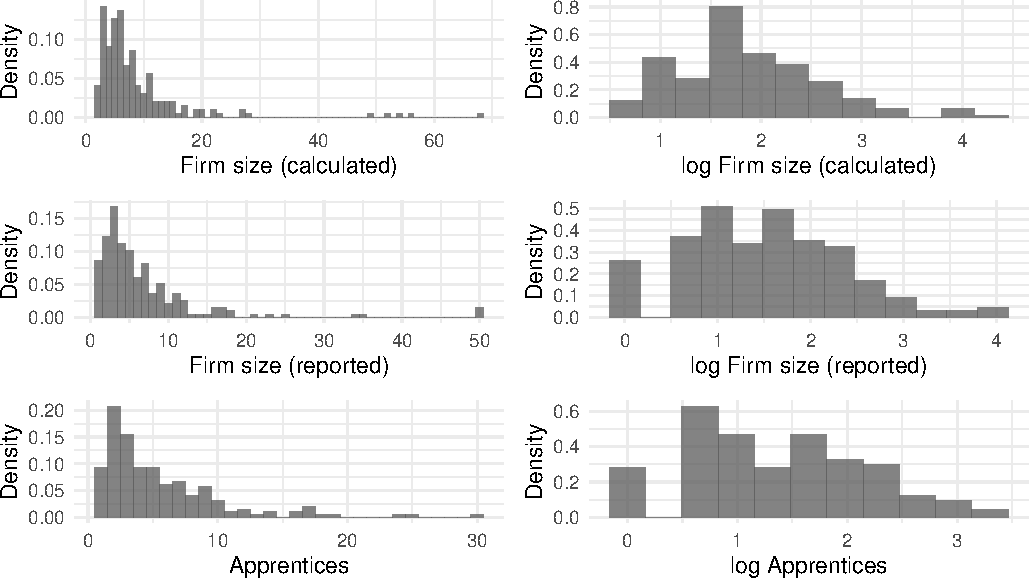
\includegraphics{figures/fig-firmsize-1} \caption{Firm size distributions}\label{fig:fig-firmsize}
\end{figure}

\end{singlespacing}

\begin{table}

\caption{\label{tab:tbl-compexp2}Competence and experience, MC vs. apprentice assessment}
\centering
\resizebox{\linewidth}{!}{
\fontsize{9}{11}\selectfont
\begin{threeparttable}
\begin{tabular}[t]{llccccc}
\toprule
\textbf{Group} & \textbf{Trade} & \textbf{N} & \textbf{Apprentice} & \textbf{N} & \textbf{Firm} & \textbf{p-value¹}\\
\midrule
Competence & Electrical Installation & 49 & 0.97 (0.06) & 46 & 0.98 (0.05) & 0.7\\
 & Masonry & 28 & 0.95 (0.08) & 28 & 0.94 (0.10) & >0.9\\
 & Carpentry & 14 & 0.92 (0.13) & 16 & 0.95 (0.08) & 0.5\\
 & Plumbing & 25 & 0.95 (0.13) & 22 & 0.92 (0.15) & 0.7\\
 & Metalwork & 21 & 0.90 (0.17) & 26 & 0.92 (0.15) & 0.4\\
 & CQP Selected & 79 & 0.95 (0.11) & 82 & 0.95 (0.11) & 0.6\\
 & CQP Not Selected & 58 & 0.95 (0.10) & 56 & 0.94 (0.10) & 0.9\\
\textbf{} & \textbf{Overall} & \textbf{137} & \textbf{0.95 (0.11)} & \textbf{138} & \textbf{0.95 (0.11)} & \textbf{0.6}\\
Experience & Electrical Installation & 49 & 0.97 (0.06) & 46 & 0.97 (0.06) & 0.9\\
 & Masonry & 28 & 0.95 (0.09) & 28 & 0.93 (0.11) & 0.9\\
 & Carpentry & 14 & 0.95 (0.12) & 16 & 0.99 (0.03) & 0.5\\
 & Plumbing & 25 & 0.98 (0.06) & 22 & 0.89 (0.17) & 0.019\\
 & Metalwork & 21 & 0.89 (0.16) & 26 & 0.89 (0.11) & 0.8\\
 & CQP Selected & 79 & 0.96 (0.10) & 82 & 0.93 (0.11) & 0.2\\
 & CQP Not Selected & 58 & 0.95 (0.09) & 56 & 0.94 (0.11) & >0.9\\
\textbf{} & \textbf{Overall} & \textbf{137} & \textbf{0.95 (0.10)} & \textbf{138} & \textbf{0.94 (0.11)} & \textbf{0.3}\\
\bottomrule
\end{tabular}
\begin{tablenotes}
\item \textit{Notes:} Mean (SD). Proportion of trade-specific tasks apprentice is deemed competent in (competence) or has already successfully attempted (experience), as reported by MC. Total of 10-15 tasks, depending on trade. Comparison only possibly at endline as apprentices were not asked to self-assess competence and experience at baseline.
\item[1] Wilcoxon rank sum test
\end{tablenotes}
\end{threeparttable}}
\end{table}

\begin{table}[H]

\caption{\label{tab:tbl-skillschangebycqp}Change in apprentice human capital scores}
\centering
\resizebox{\linewidth}{!}{
\begin{threeparttable}
\begin{tabular}[t]{lcccc}
\toprule
 & \textbf{CQP Selected}, N = 150 & \textbf{CQP Not Selected}, N = 112 & \textbf{Did Not Apply}, N = 172 & \textbf{p-value³}\\
\midrule
Competence¹ & 0.110 (0.201) & 0.060 (0.165) & 0.158 (0.325) & 0.12\\
Experience¹ & 0.148 (0.222) & 0.104 (0.207) & 0.206 (0.314) & 0.12\\
Competence¹ & 0.110 (0.201) & 0.060 (0.165) &  & 0.3\\
Experience¹ & 0.148 (0.222) & 0.104 (0.207) &  & 0.5\\
Knowledge² & 0.034 (0.185) & 0.017 (0.166) &  & 0.8\\
\bottomrule
\end{tabular}
\begin{tablenotes}
\item \textit{Notes:} Mean (SD). Change in human capital indices between baseline and endline.
\item[1] Percent of trade-specific tasks apprentice is deemed competent in (competence) or has already successfully attempted (experience), as reported by MC. Total of 10-15 tasks, depending on trade.
\item[2] Percent of trade-specific knowledge questions answered correctly by apprentice. Total of 4 or 5 questions, depending on trade.
\item[3] Analysis of variance for three groups, Wilcoxon rank sum test for two groups
\end{tablenotes}
\end{threeparttable}}
\end{table}

\begin{table}[H]

\caption{\label{tab:tbl-allowances}Monthly allowances}
\centering
\resizebox{\linewidth}{!}{
\begin{threeparttable}
\begin{tabular}[t]{llcccc}
\toprule
\textbf{Group} & \textbf{Characteristic} & \textbf{Overall}, N = 427 & \textbf{CQP Selected} & \textbf{CQP Not Selected} & \textbf{Did Not Apply}\\
\midrule
Baseline & Food & 6.66 (12.76) & 5.85 (13.54) & 8.45 (16.40) & 6.38 (10.10)\\
 & Transportation & 5.89 (18.74) & 4.67 (17.84) & 7.63 (21.45) & 5.92 (18.10)\\
 & Pocket Money & 14.68 (18.60) & 14.45 (18.62) & 16.47 (17.52) & 14.02 (19.15)\\
 & Other & 0.07 (1.06) & 0.00 (0.00) & 0.00 (0.00) & 0.14 (1.55)\\
 & Total & 27.30 (35.11) & 24.98 (37.33) & 32.55 (39.68) & 26.46 (31.20)\\
Endline & Food & 9.68 (8.04) & 7.81 (7.17) & 13.08 (7.87) & 9.17 (8.56)\\
 & Transportation & 2.91 (6.58) & 1.91 (4.24) & 3.31 (5.65) & 3.87 (9.33)\\
 & Pocket Money & 16.62 (55.33) & 18.46 (61.51) & 8.29 (16.49) & 21.49 (68.13)\\
 & Other & 0.00 (0.00) & 0.00 (0.00) & 0.00 (0.00) & 0.00 (0.00)\\
 & Total & 29.21 (54.68) & 28.18 (59.64) & 24.68 (18.43) & 34.53 (68.50)\\
Overall & Food & 7.50 (11.72) & 6.51 (11.81) & 9.98 (14.28) & 6.95 (9.84)\\
 & Transportation & 5.06 (16.35) & 3.75 (14.79) & 6.20 (17.92) & 5.50 (16.68)\\
 & Pocket Money & 15.22 (33.06) & 15.79 (38.40) & 13.78 (17.52) & 15.54 (34.97)\\
 & Other & 0.05 (0.90) & 0.00 (0.00) & 0.00 (0.00) & 0.11 (1.39)\\
 & Total & 27.83 (41.40) & 26.05 (45.76) & 29.96 (34.25) & 28.10 (41.44)\\
\bottomrule
\end{tabular}
\begin{tablenotes}
\item \textit{Notes:} Mean (SD). Amounts in \$US.
\end{tablenotes}
\end{threeparttable}}
\end{table}

\begin{singlespacing}

\begin{table}[H]

\caption{\label{tab:tbl-allowancebounds}Allowances per apprentice per year, reported by firm}
\centering
\fontsize{9}{11}\selectfont
\begin{threeparttable}
\resizebox{\linewidth}{!}{
\begin{tabular}[t]{llccc}
\toprule
Assumption & Bound & \textbf{Overall}, N = 347 & \textbf{Baseline}, N = 197 & \textbf{Endline}, N = 150\\
\midrule
\makecell[l]{12 months/year |\\ 20 days/month} & lower & 290.91 (158.68) & 284.93 (158.68) & 301.90 (158.68)\\
 & mid & 316.18 (208.26) & 304.39 (208.26) & 338.72 (208.26)\\
 & upper & 397.15 (257.85) & 384.34 (257.85) & 421.61 (257.85)\\
\makecell[l]{(F) months/year |\\ 20 days/month} & lower & 249.51 (158.68) & 238.87 (145.45) & 269.08 (158.68)\\
 & mid & 271.07 (168.60) & 256.64 (163.64) & 298.65 (197.11)\\
 & upper & 340.26 (236.36) & 324.79 (198.35) & 369.81 (257.85)\\
\makecell[l]{12 months/year |\\ 4 x (F) weeks/month} & lower & 343.66 (190.41) & 335.06 (190.41) & 359.47 (190.41)\\
 & mid & 373.36 (249.92) & 357.68 (249.92) & 403.29 (249.92)\\
 & upper & 468.69 (309.42) & 451.42 (309.42) & 501.69 (309.42)\\
\makecell[l]{(F) months/year |\\ 4 x (F) weeks/month} & lower & 297.10 (185.12) & 282.53 (174.55) & 323.87 (190.41)\\
 & mid & 322.42 (196.36) & 303.11 (180.50) & 359.30 (240.99)\\
 & upper & 404.36 (257.85) & 383.22 (226.12) & 444.73 (309.42)\\
\makecell[l]{12 months/year |\\ 4 x (A) weeks/month} & lower & 364.41 (222.15) & 337.82 (206.28) & 451.37 (222.15)\\
 & mid & 394.66 (247.60) & 360.43 (236.03) & 515.74 (291.57)\\
 & upper & 496.89 (309.42) & 455.98 (277.69) & 641.56 (360.99)\\
\makecell[l]{firm months |\\ 4 x (A) weeks/month} & lower & 317.89 (166.61) & 287.89 (166.61) & 415.98 (166.61)\\
 & mid & 344.25 (183.47) & 309.03 (180.50) & 468.83 (218.68)\\
 & upper & 432.46 (239.34) & 390.97 (206.28) & 579.15 (309.42)\\
\bottomrule
\end{tabular}}
\begin{tablenotes}
\small
\item \textit{Notes:} Mean (Median). (F): reported by firm; (A): reported by apprentices. Amounts in \$US.
\end{tablenotes}
\end{threeparttable}
\end{table}

\begin{table}[H]

\caption{\label{tab:tbl-allowboundsapp}Allowances per apprentice per year, reported by apprentice}
\centering
\fontsize{9}{11}\selectfont
\begin{threeparttable}
\resizebox{\linewidth}{!}{
\begin{tabular}[t]{llccc}
\toprule
Assumption & Bound & \textbf{Overall}, N = 347 & \textbf{Baseline}, N = 197 & \textbf{Endline}, N = 150\\
\midrule
\makecell[l]{12 months/year |\\ 4 weeks/month} & lower & 199.00 (198.35) & 187.81 (158.68) & 251.95 (238.02)\\
 & mid & 264.77 (238.02) & 252.64 (198.35) & 322.18 (317.36)\\
 & upper & 330.49 (277.61) & 317.41 (237.94) & 392.33 (396.61)\\
\makecell[l]{(F) months/year |\\ 4 weeks/month} & lower & 164.96 (119.01) & 153.26 (115.70) & 220.33 (218.18)\\
 & mid & 221.36 (158.68) & 208.59 (145.45) & 281.80 (290.91)\\
 & upper & 277.71 (198.27) & 263.87 (181.75) & 343.20 (363.56)\\
\bottomrule
\end{tabular}}
\begin{tablenotes}
\small
\item \textit{Notes:} Mean (Median). (F): reported by firm; (A): reported by apprentices. Amounts in \$US.
\end{tablenotes}
\end{threeparttable}
\end{table}

\end{singlespacing}

\begin{table}[H]

\caption{\label{tab:tbl-wages}Monthly wages}
\centering
\fontsize{9}{11}\selectfont
\begin{threeparttable}
\begin{tabular}[t]{lcccc}
\toprule
 & \textbf{N} & \textbf{Baseline} & \textbf{N} & \textbf{Endline}\\
\midrule
Former apprentice (diff. workshop) & 139 & 17 (56) & 140 & 17 (43)\\
Former apprentice (same workshop) & 139 & 19 (68) & 140 & 15 (43)\\
Worker with secondary educ. or more & 128 & 7 (35) & 140 & 9 (52)\\
Worker with primary educ. or less & 132 & 5 (30) & 140 & 4 (34)\\
Paid family worker & 124 & 4 (19) & 140 & 4 (18)\\
Occassional worker & 155 & 39 (77) & 145 & 27 (59)\\
Firm owner & 173 & 82 (88) & 144 & 124 (95)\\
Traditional apprentice (first year) & 172 & 0 (4) & 140 & 6 (10)\\
Traditional apprentice (third year) & 172 & 1 (6) & 140 & 11 (16)\\
CQP apprentice (first year) & 170 & 1 (6) & 140 & 3 (8)\\
CQP apprentice (third year) & 166 & 2 (9) & 140 & 13 (35)\\
\bottomrule
\end{tabular}
\begin{tablenotes}
\item \textit{Notes:} Mean (SD). Monthly wages in \$US.
\end{tablenotes}
\end{threeparttable}
\end{table}

\begin{figure}[H]
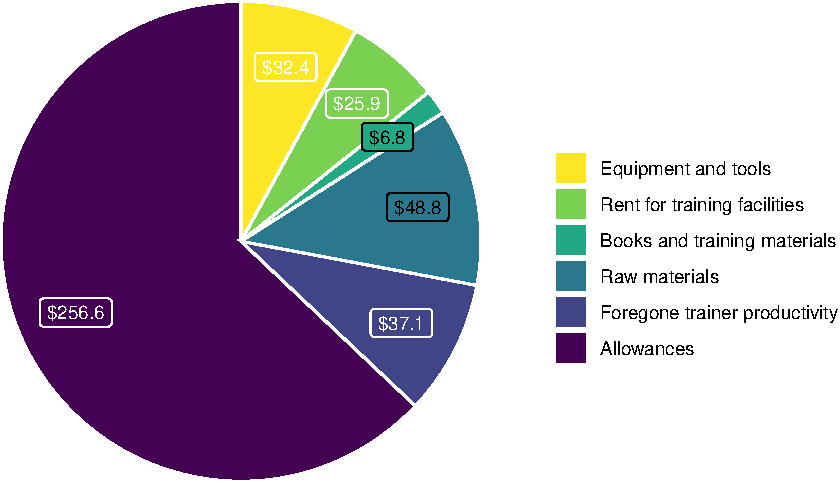
\includegraphics{figures/fig-costspie-1} \caption{Breakdown of mean annual training costs per apprentice}\label{fig:fig-costspie}
\end{figure}

\begin{figure}[H]
\includegraphics{figures/fig-costspie2-1} \caption{Breakdown of mean annual training costs per firm}\label{fig:fig-costspie2}
\end{figure}

\begin{figure}[H]
\includegraphics[width=1\linewidth,]{figures/fig-apphist-1} \caption{Distribution of net benefits per apprentice}\label{fig:fig-apphist}
\end{figure}

\begin{figure}[H]
\includegraphics[width=1\linewidth,]{figures/fig-firmhist-1} \caption{Distribution of net benefits per firm}\label{fig:fig-firmhist}
\end{figure}

\begin{table}[H]

\caption{\label{tab:tbl-appnetbenefitsnodna}Annual costs and benefits per apprentice, CQP applicants only}
\centering
\resizebox{\linewidth}{!}{
\begin{threeparttable}
\begin{tabular}[t]{lccccccc}
\toprule
\textbf{Characteristic} & \textbf{N} & \textbf{Overall} & \textbf{N} & \textbf{CQP Selected} & \textbf{N} & \textbf{CQP Not Selected} & \textbf{p-value}\\
\midrule
\addlinespace[0.3em]
\multicolumn{8}{l}{\textbf{Benefits}}\\
\hspace{1em}Fees¹ & 243 & 53.60 (37.86) & 143 & 50.74 (36.67) & 100 & 57.68 (39.33) & 0.2\\
\hspace{1em}\hspace{1em}Entry & 231 & 2.53 (4.24) & 135 & 2.33 (3.30) & 96 & 2.82 (5.29) & 0.4\\
\hspace{1em}\hspace{1em}Formation & 231 & 23.82 (30.29) & 135 & 20.10 (27.58) & 96 & 29.04 (33.19) & 0.027\\
\hspace{1em}\hspace{1em}Liberation & 231 & 8.54 (18.29) & 135 & 9.44 (18.61) & 96 & 7.26 (17.86) & 0.4\\
\hspace{1em}\hspace{1em}Materials & 231 & 6.29 (9.19) & 135 & 6.35 (9.47) & 96 & 6.20 (8.83) & >0.9\\
\hspace{1em}\hspace{1em}Contract & 231 & 10.05 (18.22) & 135 & 11.01 (18.70) & 96 & 8.70 (17.52) & 0.3\\
\hspace{1em}\hspace{1em}Application & 231 & 3.05 (4.15) & 135 & 3.30 (4.25) & 96 & 2.70 (4.00) & 0.3\\
\hspace{1em}Apprentice prod. & 62 & 1,039.62 (1,172.56) & 34 & 869.20 (1,050.46) & 28 & 1,246.57 (1,294.84) & 0.2\\
\textbf{\hspace{1em}Total} & \textbf{59} & \textbf{1,099.04 (1,195.77)} & \textbf{33} & \textbf{939.01 (1,059.45)} & \textbf{26} & \textbf{1,302.16 (1,343.08)} & \textbf{0.3}\\
\addlinespace[0.3em]
\multicolumn{8}{l}{\textbf{Costs}}\\
\hspace{1em}Allowances¹ & 235 & 604.73 (1,225.89) & 135 & 583.89 (1,398.96) & 100 & 632.85 (949.56) & 0.8\\
\hspace{1em}\hspace{1em}Food & 141 & 72.79 (171.96) & 84 & 61.57 (158.26) & 57 & 89.31 (190.63) & 0.3\\
\hspace{1em}\hspace{1em}Transport & 141 & 59.73 (205.04) & 84 & 46.23 (188.52) & 57 & 79.61 (227.49) & 0.3\\
\hspace{1em}\hspace{1em}Pocket money & 141 & 150.50 (181.49) & 84 & 135.30 (169.17) & 57 & 172.89 (197.68) & 0.2\\
\hspace{1em}\hspace{1em}Other & 141 & 0.00 (0.00) & 84 & 0.00 (0.00) & 57 & 0.00 (0.00) & \\
\hspace{1em}Training costs & 147 & 126.35 (250.66) & 88 & 110.95 (251.60) & 59 & 149.32 (249.61) & 0.4\\
\hspace{1em}\hspace{1em}Rent & 147 & 30.89 (65.54) & 88 & 24.18 (52.84) & 59 & 40.90 (80.34) & 0.13\\
\hspace{1em}\hspace{1em}Equipment & 144 & 36.96 (90.62) & 88 & 24.75 (50.81) & 56 & 56.15 (129.04) & 0.042\\
\hspace{1em}\hspace{1em}Books & 143 & 9.48 (45.27) & 87 & 7.65 (40.66) & 56 & 12.32 (51.90) & 0.5\\
\hspace{1em}\hspace{1em}Raw materials & 142 & 51.79 (161.19) & 87 & 55.07 (187.93) & 55 & 46.60 (107.48) & 0.8\\
\hspace{1em}Lost trainer prod. & 141 & 34.69 (43.60) & 83 & 37.68 (47.11) & 58 & 30.40 (38.00) & 0.3\\
\textbf{\hspace{1em}Total} & \textbf{66} & \textbf{758.45 (730.85)} & \textbf{39} & \textbf{676.45 (673.07)} & \textbf{27} & \textbf{876.90 (805.36)} & \textbf{0.3}\\
\addlinespace[0.3em]
\multicolumn{8}{l}{\textbf{Net Benefits}}\\
\hspace{1em}Model I & 223 & -564.88 (1,254.43) & 130 & -547.64 (1,422.47) & 93 & -588.98 (979.25) & 0.8\\
\hspace{1em}Model II & 133 & -598.70 (725.90) & 79 & -571.18 (764.74) & 54 & -638.96 (670.01) & 0.6\\
\hspace{1em}Model III & 53 & 610.97 (1,312.97) & 29 & 444.72 (1,169.03) & 24 & 811.85 (1,468.62) & 0.3\\
\hspace{1em}Model IV & 24 & 644.01 (1,566.27) & 12 & 78.33 (1,264.37) & 12 & 1,209.68 (1,683.05) & 0.076\\
\hspace{1em}Model V & 21 & 721.95 (1,555.49) & 11 & -8.33 (1,298.95) & 10 & 1,525.25 (1,460.55) & 0.020\\
\bottomrule
\end{tabular}
\begin{tablenotes}
\small
\item \textit{Notes:} Mean (SD). Amounts in \$US per apprentice per year, calculated using responses from baseline survey.
\item[1] Fees and allowances reported by firm owner. Annual fees assume apprenticeship duration of four years, annual allowances assume apprentices work 20 days a month.
\end{tablenotes}
\end{threeparttable}}
\end{table}

\begin{table}[H]

\caption{\label{tab:tbl-appnetbenefitsbywave}Annual costs and benefits per apprentice, by wave}
\centering
\resizebox{\linewidth}{!}{
\begin{threeparttable}
\begin{tabular}[t]{lccccccc}
\toprule
 & \textbf{N} & \textbf{Overall} & \textbf{N} & \textbf{Baseline} & \textbf{N} & \textbf{Endline} & \textbf{p-value}\\
\midrule
\addlinespace[0.3em]
\multicolumn{8}{l}{\textbf{Benefits}}\\
\hspace{1em}Fees¹ & 591 & 64.73 (43.35) & 403 & 65.30 (44.66) & 188 & 63.51 (40.49) & 0.9\\
\hspace{1em}\hspace{1em}Entry & 579 & 3.11 (6.23) & 391 & 2.74 (4.11) & 188 & 3.90 (9.15) & 0.2\\
\hspace{1em}\hspace{1em}Formation & 579 & 36.05 (38.19) & 391 & 35.95 (38.04) & 188 & 36.26 (38.61) & 0.6\\
\hspace{1em}\hspace{1em}Liberation & 579 & 9.19 (20.76) & 391 & 9.26 (18.70) & 188 & 9.03 (24.54) & 0.012\\
\hspace{1em}\hspace{1em}Materials & 579 & 6.07 (8.16) & 391 & 6.56 (9.31) & 188 & 5.07 (4.85) & 0.4\\
\hspace{1em}\hspace{1em}Contract & 579 & 7.30 (15.69) & 391 & 8.46 (16.92) & 188 & 4.87 (12.43) & 0.020\\
\hspace{1em}\hspace{1em}Application & 579 & 3.51 (4.18) & 391 & 3.09 (4.24) & 188 & 4.38 (3.93) & <0.001\\
\hspace{1em}Apprentice prod. & 241 & 760.05 (977.48) & 114 & 1,075.59 (1,172.98) & 127 & 476.80 (644.26) & <0.001\\
\textbf{\hspace{1em}Total} & \textbf{203} & \textbf{841.72 (996.42)} & \textbf{104} & \textbf{1,140.89 (1,198.06)} & \textbf{99} & \textbf{527.44 (585.80)} & \textbf{<0.001}\\
\addlinespace[0.3em]
\multicolumn{8}{l}{\textbf{Costs}}\\
\hspace{1em}Allowances¹ & 470 & 463.58 (955.16) & 360 & 489.37 (1,021.21) & 110 & 379.17 (693.82) & 0.023\\
\hspace{1em}\hspace{1em}Food & 368 & 77.08 (134.55) & 266 & 70.57 (147.07) & 102 & 94.05 (92.90) & <0.001\\
\hspace{1em}\hspace{1em}Transport & 368 & 52.46 (170.87) & 266 & 60.88 (195.20) & 102 & 30.51 (73.78) & >0.9\\
\hspace{1em}\hspace{1em}Pocket money & 368 & 157.37 (380.71) & 266 & 145.96 (183.74) & 102 & 187.12 (660.95) & 0.001\\
\hspace{1em}\hspace{1em}Other & 368 & 0.47 (9.05) & 266 & 0.65 (10.64) & 102 & 0.00 (0.00) & 0.5\\
\hspace{1em}Training costs & 466 & 109.15 (219.01) & 229 & 110.69 (233.24) & 237 & 107.65 (204.80) & >0.9\\
\hspace{1em}\hspace{1em}Rent & 466 & 28.54 (63.68) & 229 & 26.83 (59.79) & 237 & 30.20 (67.31) & >0.9\\
\hspace{1em}\hspace{1em}Equipment & 460 & 32.38 (75.06) & 226 & 32.61 (81.94) & 234 & 32.16 (67.92) & 0.8\\
\hspace{1em}\hspace{1em}Books & 456 & 8.80 (41.76) & 224 & 8.93 (44.17) & 232 & 8.68 (39.40) & >0.9\\
\hspace{1em}\hspace{1em}Raw materials & 454 & 41.08 (135.13) & 223 & 44.10 (140.23) & 231 & 38.16 (130.26) & >0.9\\
\hspace{1em}Lost trainer prod. & 331 & 33.60 (45.59) & 245 & 36.08 (45.78) & 86 & 26.54 (44.52) & 0.12\\
\textbf{\hspace{1em}Total} & \textbf{135} & \textbf{622.24 (647.58)} & \textbf{96} & \textbf{666.56 (698.44)} & \textbf{39} & \textbf{513.15 (492.00)} & \textbf{0.2}\\
\addlinespace[0.3em]
\multicolumn{8}{l}{\textbf{Net Benefits}}\\
\hspace{1em}Model I & 442 & -404.86 (980.27) & 341 & -437.12 (1,047.68) & 101 & -295.95 (700.14) & 0.011\\
\hspace{1em}Model II & 299 & -454.58 (679.06) & 198 & -480.28 (661.41) & 101 & -404.20 (713.08) & 0.2\\
\hspace{1em}Model III & 132 & 403.62 (1,203.22) & 75 & 726.77 (1,275.80) & 57 & -21.58 (954.96) & 0.003\\
\hspace{1em}Model IV & 88 & 121.25 (1,180.94) & 31 & 631.55 (1,406.07) & 57 & -156.28 (940.73) & 0.005\\
\hspace{1em}Model V & 54 & 295.69 (1,111.39) & 28 & 686.67 (1,378.91) & 26 & -125.38 (457.68) & 0.012\\
\bottomrule
\end{tabular}
\begin{tablenotes}
\small
\item \textit{Notes:} Mean (SD). Amounts in \$US per apprentice per year, calculated using responses from baseline survey.
\item[1] Fees and allowances reported by firm owner. Annual fees assume apprenticeship duration of four years, annual allowances assume apprentices work 20 days a month.
\end{tablenotes}
\end{threeparttable}}
\end{table}

\begin{landscape}
\begin{singlespacing}
\begin{table}[H]

\caption{\label{tab:tbl-appnetbenefitsbytrade}Annual costs and benefits per apprentice, by trade}
\centering
\resizebox{\linewidth}{!}{
\begin{threeparttable}
\begin{tabular}[t]{lccccccc}
\toprule
\multicolumn{2}{c}{ } & \multicolumn{5}{c}{\textbf{Trade}} & \multicolumn{1}{c}{ } \\
\cmidrule(l{3pt}r{3pt}){3-7}
 & \textbf{Overall} & \textbf{Masonry} & \textbf{Carpentry} & \textbf{Plumbing} & \textbf{Metalwork} & \textbf{Electrical Inst.} & \textbf{p-value}\\
\midrule
\addlinespace[0.3em]
\multicolumn{8}{l}{\textbf{Benefits}}\\
\hspace{1em}Fees¹ & 65.30 (44.66) & 70.17 (38.53) & 56.97 (42.03) & 49.98 (28.28) & 52.06 (44.50) & 78.34 (49.66) & <0.001\\
\hspace{1em}\hspace{1em}Entry & 2.74 (4.11) & 1.80 (2.65) & 1.74 (2.18) & 2.47 (3.58) & 1.05 (1.75) & 4.62 (5.45) & <0.001\\
\hspace{1em}\hspace{1em}Formation & 35.95 (38.04) & 36.74 (29.00) & 33.28 (30.91) & 21.31 (32.39) & 27.26 (33.17) & 46.84 (45.52) & <0.001\\
\hspace{1em}\hspace{1em}Liberation & 9.26 (18.70) & 15.04 (20.84) & 9.87 (17.95) & 1.99 (5.77) & 7.81 (17.74) & 9.38 (20.44) & 0.001\\
\hspace{1em}\hspace{1em}Materials & 6.56 (9.31) & 8.39 (9.26) & 5.34 (5.86) & 2.89 (3.35) & 7.16 (12.96) & 6.90 (8.88) & <0.001\\
\hspace{1em}\hspace{1em}Contract & 8.46 (16.92) & 3.68 (10.44) & 7.78 (17.15) & 19.21 (22.95) & 6.74 (14.86) & 8.24 (16.72) & 0.3\\
\hspace{1em}\hspace{1em}Application & 3.09 (4.24) & 4.62 (3.96) & 4.39 (4.09) & 2.10 (3.72) & 2.99 (3.98) & 2.28 (4.48) & <0.001\\
\hspace{1em}Apprentice prod. & 1,075.59 (1,172.98) & 1,480.90 (1,306.63) & 1,118.65 (1,328.96) & 1,666.12 (298.76) & 482.72 (382.95) & 819.63 (1,087.83) & <0.001\\
\textbf{\hspace{1em}Total} & \textbf{1,140.89 (1,198.06)} & \textbf{1,683.73 (1,396.03)} & \textbf{1,013.33 (1,182.41)} & \textbf{1,694.46 (319.67)} & \textbf{537.43 (366.98)} & \textbf{884.07 (1,110.78)} & \textbf{<0.001}\\
\addlinespace[0.3em]
\multicolumn{8}{l}{\textbf{Costs}}\\
\hspace{1em}Allowances¹ & 489.37 (1,021.21) & 502.98 (868.71) & 264.34 (237.20) & 429.50 (708.59) & 264.85 (342.57) & 749.79 (1,564.54) & <0.001\\
\hspace{1em}\hspace{1em}Food & 70.57 (147.07) & 82.21 (82.86) & 34.68 (54.89) & 38.02 (67.32) & 68.44 (79.16) & 99.56 (266.47) & <0.001\\
\hspace{1em}\hspace{1em}Transport & 60.88 (195.20) & 49.33 (84.00) & 46.62 (65.40) & 57.22 (82.98) & 4.39 (26.35) & 133.42 (369.79) & <0.001\\
\hspace{1em}\hspace{1em}Pocket money & 145.96 (183.74) & 230.00 (228.63) & 101.14 (114.89) & 80.15 (68.54) & 90.81 (147.42) & 169.81 (201.63) & <0.001\\
\hspace{1em}\hspace{1em}Other & 0.65 (10.64) & 0.00 (0.00) & 0.00 (0.00) & 0.00 (0.00) & 0.00 (0.00) & 2.71 (21.69) & 0.5\\
\hspace{1em}Training costs & 110.69 (233.24) & 139.64 (200.16) & 126.09 (339.41) & 52.95 (99.52) & 75.19 (107.92) & 137.34 (289.99) & 0.090\\
\hspace{1em}\hspace{1em}Rent & 26.83 (59.79) & 18.82 (40.33) & 3.99 (9.65) & 6.31 (26.40) & 28.76 (47.40) & 45.48 (83.14) & <0.001\\
\hspace{1em}\hspace{1em}Equipment & 32.61 (81.94) & 68.13 (140.03) & 6.60 (18.41) & 21.98 (39.25) & 11.26 (25.83) & 41.26 (86.88) & <0.001\\
\hspace{1em}\hspace{1em}Books & 8.93 (44.17) & 8.29 (25.58) & 0.35 (1.78) & 6.90 (14.26) & 0.00 (0.00) & 18.30 (71.27) & 0.006\\
\hspace{1em}\hspace{1em}Raw materials & 44.10 (140.23) & 44.40 (73.39) & 115.15 (325.67) & 17.76 (51.85) & 35.17 (78.39) & 37.61 (113.62) & 0.030\\
\hspace{1em}Lost trainer prod. & 36.08 (45.78) & 34.05 (34.14) & 62.78 (76.69) & 53.48 (59.14) & 27.94 (30.68) & 31.36 (48.34) & 0.4\\
\textbf{\hspace{1em}Total} & \textbf{666.56 (698.44)} & \textbf{648.85 (324.48)} & \textbf{479.98 (618.49)} & \textbf{551.68 (594.94)} & \textbf{337.80 (222.65)} & \textbf{1,191.18 (1,084.98)} & \textbf{<0.001}\\
\addlinespace[0.3em]
\multicolumn{8}{l}{\textbf{Net Benefits}}\\
\hspace{1em}Model I & -437.12 (1,047.68) & -450.07 (917.78) & -216.41 (251.65) & -378.49 (710.13) & -215.64 (353.20) & -682.98 (1,580.38) & 0.001\\
\hspace{1em}Model II & -480.28 (661.41) & -468.88 (294.90) & -304.93 (417.16) & -464.94 (817.96) & -263.52 (221.37) & -659.02 (849.99) & 0.019\\
\hspace{1em}Model III & 726.77 (1,275.80) & 1,186.96 (1,374.17) & 741.15 (1,073.05) & 1,424.71 (275.21) & -228.78 (682.42) & 164.80 (1,177.03) & 0.001\\
\hspace{1em}Model IV & 631.55 (1,406.07) & 822.50 (1,449.81) & 148.02 (1,560.68) & 1,273.66 (163.37) & -82.23 (291.90) & 465.08 (1,747.39) & 0.4\\
\hspace{1em}Model V & 686.67 (1,378.91) & 830.37 (1,575.09) & 122.88 (1,602.28) & 1,254.03 (141.56) & -107.30 (320.73) & 703.77 (1,563.70) & 0.6\\
\bottomrule
\end{tabular}
\begin{tablenotes}
\small
\item \textit{Notes:} Mean (SD). Amounts in \$US per apprentice per year, calculated using responses from baseline survey.
\item[1] Fees and allowances reported by firm owner. Annual fees assume apprenticeship duration of four years, annual allowances assume apprentices work 20 days a month.
\end{tablenotes}
\end{threeparttable}}
\end{table}
\end{singlespacing}
\end{landscape}

\begin{table}[H]

\caption{\label{tab:tbl-firmnetbenefitsbywave}Annual net benefits per firm, by wave}
\centering
\resizebox{\linewidth}{!}{
\begin{threeparttable}
\begin{tabular}[t]{lccccccc}
\toprule
 & \textbf{N} & \textbf{Overall} & \textbf{N} & \textbf{Baseline} & \textbf{N} & \textbf{Endline} & \textbf{p-value}\\
\midrule
\addlinespace[0.3em]
\multicolumn{8}{l}{\textbf{Firm Accounts}}\\
\hspace{1em}Revenues & 300 & 4,405 (4,917) & 159 & 3,989 (4,820) & 141 & 4,875 (5,000) & 0.002\\
\hspace{1em}Wage bill & 344 & 1,365 (2,999) & 196 & 972 (2,352) & 148 & 1,886 (3,629) & <0.001\\
\hspace{1em}Non-wage expenses & 342 & 1,640 (3,179) & 196 & 1,593 (3,152) & 146 & 1,704 (3,224) & 0.2\\
\hspace{1em}Total expenses & 340 & 3,027 (5,183) & 195 & 2,572 (4,453) & 145 & 3,639 (5,989) & <0.001\\
\hspace{1em}Profits (reported) & 303 & 1,429 (2,159) & 167 & 1,672 (2,634) & 136 & 1,132 (1,317) & 0.029\\
\hspace{1em}Profits (calculated²) & 297 & 1,549 (3,249) & 158 & 1,701 (3,056) & 139 & 1,375 (3,459) & 0.7\\
\addlinespace[0.3em]
\multicolumn{8}{l}{\textbf{Projected benefits}}\\
\hspace{1em}Fees & 317 & 370 (451) & 189 & 347 (366) & 128 & 403 (553) & >0.9\\
\hspace{1em}Apprentice prod. & 128 & 5,655 (13,455) & 47 & 8,359 (13,033) & 81 & 4,086 (13,526) & 0.011\\
\hspace{1em}Total & 117 & 6,063 (13,708) & 46 & 8,887 (13,241) & 71 & 4,234 (13,786) & 0.011\\
\addlinespace[0.3em]
\multicolumn{8}{l}{\textbf{Projected costs}}\\
\hspace{1em}Allowances & 269 & 2,783 (6,783) & 185 & 3,207 (7,741) & 84 & 1,848 (3,803) & 0.006\\
\hspace{1em}Training costs & 292 & 497 (1,071) & 144 & 511 (1,116) & 148 & 483 (1,029) & >0.9\\
\hspace{1em}Lost trainer prod. & 169 & 199 (506) & 111 & 181 (421) & 58 & 233 (640) & 0.6\\
\hspace{1em}Total & 103 & 3,430 (4,838) & 70 & 3,190 (4,441) & 33 & 3,938 (5,628) & 0.6\\
\addlinespace[0.3em]
\multicolumn{8}{l}{\textbf{Net benefits}}\\
\hspace{1em}Model I & 258 & -2,500 (6,838) & 180 & -2,947 (7,759) & 78 & -1,469 (3,814) & 0.005\\
\hspace{1em}Model II & 206 & -2,681 (7,150) & 128 & -3,174 (8,534) & 78 & -1,870 (3,861) & 0.034\\
\hspace{1em}Model III & 86 & 2,773 (9,640) & 43 & 5,574 (12,052) & 43 & -28 (5,171) & 0.10\\
\hspace{1em}Model IV & 68 & 2,040 (9,146) & 25 & 6,431 (12,457) & 43 & -513 (5,158) & 0.034\\
\hspace{1em}Model V & 43 & 2,717 (10,714) & 23 & 6,593 (12,285) & 20 & -1,740 (6,316) & 0.013\\
\bottomrule
\end{tabular}
\begin{tablenotes}
\small
\item \textit{Notes:} Mean (SD). Net benefits per firm estimated using baseline data. 
Projected costs, benefits, and net benefits calculated as mean values for all observed apprentices in 
firm times reported number of apprentices trained. Amounts in \$US.
\item[1] Firms size calculated by author as sum of all reported workers in firm, including apprentices and occasional and family workers.
\item[2] Profits recalculated by author as difference between reported revenues (first row) and reported expenses (second row).
\end{tablenotes}
\end{threeparttable}}
\end{table}

\begin{landscape}

\begin{table}[H]

\caption{\label{tab:tbl-firmnetbenefitsbytrade}Annual net benefits per firm, by trade}
\centering
\resizebox{\linewidth}{!}{
\begin{threeparttable}
\begin{tabular}[t]{lccccccc}
\toprule
\multicolumn{2}{c}{ } & \multicolumn{5}{c}{\textbf{Trade}} & \multicolumn{1}{c}{ } \\
\cmidrule(l{3pt}r{3pt}){3-7}
 & \textbf{Overall}, N = 197 & \textbf{Masonry}, N = 45 & \textbf{Carpentry}, N = 24 & \textbf{Plumbing}, N = 26 & \textbf{Metalwork}, N = 39 & \textbf{Electrical Inst.}, N = 63 & \textbf{p-value}\\
\midrule
\addlinespace[0.3em]
\multicolumn{8}{l}{\textbf{Firm Accounts}}\\
\hspace{1em}Revenues & 3,989 (4,820) & 4,924 (5,760) & 4,999 (4,256) & 2,696 (3,246) & 3,498 (4,993) & 3,477 (4,447) & 0.021\\
\hspace{1em}Wage bill & 972 (2,352) & 2,304 (4,254) & 880 (1,392) & 642 (1,182) & 277 (560) & 609 (1,147) & <0.001\\
\hspace{1em}Non-wage expenses & 1,593 (3,152) & 1,318 (2,216) & 1,415 (1,757) & 653 (828) & 1,131 (1,338) & 2,528 (4,882) & 0.016\\
\hspace{1em}Total expenses & 2,572 (4,453) & 3,622 (5,559) & 2,333 (2,835) & 1,295 (1,770) & 1,411 (1,607) & 3,138 (5,639) & 0.002\\
\hspace{1em}Profits (reported) & 1,672 (2,634) & 2,567 (4,557) & 2,243 (1,408) & 1,202 (1,428) & 1,007 (1,381) & 1,266 (1,158) & <0.001\\
\hspace{1em}Profits (calculated²) & 1,701 (3,056) & 1,243 (2,957) & 2,569 (2,369) & 1,449 (1,506) & 1,967 (4,672) & 1,662 (2,572) & 0.14\\
\addlinespace[0.3em]
\multicolumn{8}{l}{\textbf{Projected benefits}}\\
\hspace{1em}Fees & 347 (366) & 317 (256) & 212 (178) & 219 (195) & 273 (332) & 526 (485) & <0.001\\
\hspace{1em}Apprentice prod. & 8,359 (13,033) & 8,719 (11,196) & 11,109 (22,156) & 9,124 (2,244) & 4,161 (6,282) & 7,990 (13,047) & 0.4\\
\hspace{1em}Total & 8,887 (13,241) & 9,472 (11,545) & 11,347 (22,106) & 9,235 (2,157) & 4,531 (6,864) & 8,542 (13,216) & 0.4\\
\addlinespace[0.3em]
\multicolumn{8}{l}{\textbf{Projected costs}}\\
\hspace{1em}Allowances & 3,207 (7,741) & 2,529 (3,775) & 1,640 (2,966) & 4,733 (17,348) & 1,541 (2,198) & 4,865 (6,332) & <0.001\\
\hspace{1em}Training costs & 511 (1,116) & 532 (723) & 404 (564) & 215 (367) & 341 (659) & 792 (1,739) & 0.2\\
\hspace{1em}Lost trainer prod. & 181 (421) & 148 (200) & 408 (1,038) & 254 (477) & 96 (92) & 194 (435) & >0.9\\
\hspace{1em}Total & 3,190 (4,441) & 3,144 (2,226) & 1,236 (854) & 2,009 (2,835) & 1,910 (3,123) & 6,173 (7,359) & 0.005\\
\addlinespace[0.3em]
\multicolumn{8}{l}{\textbf{Net benefits}}\\
\hspace{1em}Model I & -2,947 (7,759) & -2,373 (3,872) & -1,470 (3,004) & -4,515 (17,220) & -1,245 (2,052) & -4,454 (6,299) & 0.004\\
\hspace{1em}Model II & -3,174 (8,534) & -2,748 (2,869) & -995 (910) & -5,419 (19,345) & -1,465 (2,461) & -4,325 (5,315) & <0.001\\
\hspace{1em}Model III & 5,574 (12,052) & 6,553 (9,848) & 8,494 (17,498) & 7,780 (1,858) & 291 (4,639) & 4,190 (13,916) & 0.3\\
\hspace{1em}Model IV & 6,431 (12,457) & 7,385 (11,698) & 2,772 (7,030) & 7,368 (2,441) & 767 (1,901) & 7,792 (17,945) & 0.8\\
\hspace{1em}Model V & 6,593 (12,285) & 6,835 (12,160) & 2,733 (7,067) & 7,290 (2,552) & 682 (1,909) & 9,426 (17,584) & 0.8\\
\bottomrule
\end{tabular}
\begin{tablenotes}
\small
\item \textit{Notes:} Mean (SD). Net benefits per firm estimated using baseline data. 
Projected costs, benefits, and net benefits calculated as mean values for all observed apprentices in 
firm times reported number of apprentices trained. Amounts in \$US.
\item[1] Firms size calculated by author as sum of all reported workers in firm, including apprentices and occasional and family workers.
\item[2] Profits recalculated by author as difference between reported revenues (first row) and reported expenses (second row).
\end{tablenotes}
\end{threeparttable}}
\end{table}

\end{landscape}

\begin{table}[H] \centering 
  \caption{Firm-level regressions with firm fixed effects} 
  \label{tab:firmregsfe} 
\footnotesize 
\begin{tabular}{@{\extracolsep{5pt}}lcccccc} 
\\[-1.8ex]\hline 
\hline \\[-1.8ex] 
\\[-1.8ex] & \multicolumn{2}{c}{log revenues (USD)} & \multicolumn{2}{c}{log profits (USD)} & \multicolumn{2}{c}{log Firm size$^1$} \\ 
\\[-1.8ex] & (1) & (2) & (3) & (4) & (5) & (6)\\ 
\hline \\[-1.8ex] 
 Non-CQP apprentices & $-$0.01 &  & $-$0.93$^{**}$ &  & $-$0.33$^{*}$ &  \\ 
  & (0.21) &  & (0.37) &  & (0.18) &  \\ 
  CQP Selected &  & $-$0.11 &  & $-$0.94$^{**}$ &  & $-$0.33$^{**}$ \\ 
  &  & (0.18) &  & (0.38) &  & (0.16) \\ 
  Total apprentices & 0.38$^{*}$ & 0.36$^{*}$ & $-$2.10$^{***}$ & $-$2.00$^{***}$ & $-$0.20 & $-$0.30$^{*}$ \\ 
  & (0.20) & (0.19) & (0.48) & (0.48) & (0.15) & (0.15) \\ 
  Endline & 0.32 & 0.30 & $-$0.88 & $-$1.00 &  &  \\ 
  & (0.24) & (0.23) & (0.78) & (0.77) &  &  \\ 
 \hline \\[-1.8ex] 
Firm FE & YES & YES & YES & YES & YES & YES \\ 
Observations & 126 & 134 & 94 & 101 & 143 & 156 \\ 
R$^{2}$ & 0.20 & 0.24 & 0.74 & 0.69 & 0.11 & 0.14 \\ 
F Statistic & 1.90 & 2.60$^{*}$ & 6.50$^{**}$ & 6.00$^{**}$ & 2.00 & 3.20$^{*}$ \\ 
\hline 
\hline \\[-1.8ex] 
\multicolumn{7}{l}{$^{*}$p$<$0.1; $^{**}$p$<$0.05; $^{***}$p$<$0.01} \\ 
\multicolumn{7}{l}{\textit{Notes:} $^1$Excluding apprentices} \\ 
\end{tabular} 
\end{table}

\newpage

\hypertarget{cqp-appendix-b}{%
\section*{Appendix B4}\label{cqp-appendix-b}}
\addcontentsline{toc}{section}{Appendix B4}

\markboth{Appendix B4}{Appendix B4}

\setcounter{figure}{0}
\renewcommand{\thefigure}{B4.\arabic{figure}}
\setcounter{table}{0}
\renewcommand{\thetable}{B4.\arabic{table}}

\begin{longtable}[]{@{}
  >{\raggedright\arraybackslash}p{(\columnwidth - 2\tabcolsep) * \real{0.5000}}
  >{\raggedright\arraybackslash}p{(\columnwidth - 2\tabcolsep) * \real{0.5000}}@{}}
\caption{\label{tab:tasks} Tasks used for assessment of competence and experience}\tabularnewline
\toprule\noalign{}
\begin{minipage}[b]{\linewidth}\raggedright
French
\end{minipage} & \begin{minipage}[b]{\linewidth}\raggedright
English
\end{minipage} \\
\midrule\noalign{}
\endfirsthead
\toprule\noalign{}
\begin{minipage}[b]{\linewidth}\raggedright
French
\end{minipage} & \begin{minipage}[b]{\linewidth}\raggedright
English
\end{minipage} \\
\midrule\noalign{}
\endhead
\bottomrule\noalign{}
\endlastfoot
\textbf{Masonry} & \\
Lecture d'un plan de construction & Reading a building plan \\
Identification des différents types de briques & Identifying different types of bricks \\
Composition du béton de fondation & Composition of foundation concrete \\
Composition du béton de la dalle & Composition of slab concrete \\
Élévation & Drafting an elevation \\
Chaînage bas & Low trussing \\
Chaînage haut & High trussing \\
Réalisation des pentes & Pouring out inclined surface \\
Pose des hourdis & Laying down slabs \\
Réalisation des poutres & Installing beams \\
Réalisation des feuillures & Installing rabbets \\
Cimentage du plafond & Cementing a ceiling \\
Cimentage du sol & Cementing a floor \\
Pose des chapes & Laying the floorboards \\
Réalisation d'un devis pour une construction & Drawing up an estimate \\
----------------------------------------------------------- & --------------------------------------------------------- \\
\textbf{Carpentry} & \\
Prise de mesure des portes et fenêtres & Measurement of doors and windows \\
Prise de mesure des tables et chaises & Measurement of tables and chairs \\
Pointage du bois & Scoring of wood \\
Rabotage & Planing \\
Ponçage & Sanding \\
Savoir faire le mastic & Knowing ho to make sealant \\
Assemblage pour la construction d'une chaise & Chair assembly \\
Assemblage pour la construction d'une table & Table assembly \\
Identification des différents bois utilisés & Identification of different woods used \\
Identification des différentes coupures de bois & Identification of different wood cuts \\
Réalisation de devis pour un produit & Drawing up an estimate for a product \\
----------------------------------------------------------- & --------------------------------------------------------- \\
\textbf{Plumbing} & \\
Lecture d'un plan de plomberie & Reading a plumbing plan \\
Grattage de tuyau & Pipe scraping \\
Collage des raccords & Attachment of fittings \\
Pose des tuyaux & Laying of pipes \\
Réservation des attentes aux poteaux & Securing pipes at the posts \\
Canalisation des tuyaux dans les fausses septiques et puisards & Piping in septic tanks and sumps \\
Canalisation d'un bâtiment & Piping a building \\
Canalisation pour l'alimentation en eau froide & Piping for cold water supply \\
Réalisation d'un devis & Drawing up an estimate \\
Pose apparente des appareils sanitaires & Installation of exposed sanitary appliances \\
----------------------------------------------------------- & --------------------------------------------------------- \\
\textbf{Metalworking} & \\
Lecture du plan de construction de l'ouvrage & Reading a construction plan \\
Identification des types de feuilles de tôles & Identifying different types of sheet metal \\
Identification des types de barres de fer & Identifying the different types of iron bars \\
Prise de mesure des feuilles de tôles & Measuring the sheet metal \\
Découpage des feuilles de tôles pour la formation de la charpente & Cutting of sheet metal for the frame \\
Prise de mesure pour la formation des fenêtres & Window measurements \\
Prise de mesure pour la formation des portails & Gate measurements \\
Prise de mesure pour la formation des charpentes & Frame measurement \\
Réalisation des cadres pour les fenêtres & Making the frames for the windows \\
Réalisation des cadres pour les portails & Making the frames for the gates \\
Pose des serrures & Fitting the locks \\
Assemblage des feuilles de tôles pour la formation des fenêtres & Assembly of sheet metal for windows \\
Assemblage des feuilles de tôles pour la formation des portails & Assembly of sheet metal for gates \\
Assemblage des feuilles de tôles pour la réalisation des charpentes & Assembly of sheet metal for joining of frames \\
Réalisation d'un devis pour un ouvrage & Drawing up an estimate \\
--------------------------------------------------------- & --------------------------------------------------------- \\
\textbf{Electrical Inst.} & \\
Lecture d'un plan d'électricité & Reading an electrical plan \\
Conception d'un plan d'électricité & Designing an electrical plan \\
Installation du barrage de terre & Installing an earth barrier \\
Tubage du sol & Soil casing \\
Tubage de la dalle & Tubing the floor slab \\
Serrage des boîtiers et coffrets & Clamping of boxes and cabinets \\
Pose des lampes & Installation of lamps \\
Pose des prises & Installation of sockets \\
Installation des disjoncteurs dans les coffrets & Installation of circuit breakers \\
Réalisation d'un devis & Drawing up an estimate \\
\end{longtable}

\begin{singlespacing}

\begin{figure}[H]
\includegraphics{figures/questionnaire/metalworking} \caption{\label{fig:metalworkers}Questions for metal workers}\label{fig:unnamed-chunk-6}
\end{figure}

\begin{figure}[H]
\includegraphics{figures/questionnaire/plumbing} \caption{\label{fig:qs_plumbers}Questions for plumbers}\label{fig:unnamed-chunk-7}
\end{figure}

\begin{figure}[H]
\includegraphics{figures/questionnaire/carpentry} \caption{\label{fig:qs_carpenters}Questions for carpenters}\label{fig:unnamed-chunk-8}
\end{figure}

\begin{figure}[H]
\includegraphics{figures/questionnaire/masonry} \caption{\label{fig:qs_masons}Questions for masons}\label{fig:unnamed-chunk-9}
\end{figure}

\begin{figure}[H]
\includegraphics{figures/questionnaire/electricians} \caption{\label{fig:qs_electricians}Questions for electricians}\label{fig:unnamed-chunk-10}
\end{figure}
\end{singlespacing}

\renewcommand{\thesection}{\arabic{chapter}.\arabic{section}}
\setcounter{section}{0}
\renewcommand{\thesubsection}{\arabic{chapter}.\arabic{section}.\arabic{subsection}}
\setcounter{subsection}{0}

\newsection

\chapter{Conclusion}

\hl{In summary, this thesis illuminates the school-to-work transition at both the national and individual level, and evaluates one program that attempts to ease this transition by combining training and classroom education. Our research highlights the critical link between demographics and labor market strength, while challenging the common wisdom that labor market strength is necessarily correlated with GDP. Moreover, it shows that youth in a highly informal, highly urban labor market experience school-to-work transitions that may be more akin to those measured in high-income countries than those experienced by the average person in the region, with the notable exception of young women, who are shown to be highly disadvantaged in the process. Finally, our study of dual training in the informal apprenticeship system suggests that informal apprenticeships significantly improve skills on average, while the addition of a formal dual education component yields few additional benefits. We reiterate and summarize the main findings and make suggestions for future research below, and close with policy recommendations.}

\hypertarget{section-5}{%
\section{\texorpdfstring{\hl{Revisiting the Main Findings and Future Research Outlook}}{}}\label{section-5}}

\hypertarget{section-6}{%
\subsubsection*{\texorpdfstring{\hl{Paper 1: Youth Labor Index for Low Income Countries}}{}}\label{section-6}}

\hl{Paper 1 of this dissertation introduces the Youth Labor Market Index for Low-Income Countries (YLILI), a novel composite index designed to provide a more comprehensive picture of youth labor market strength compared to single indicators such as the unemployment rate. The YLILI incorporates three key dimensions: education, working conditions, and transition smoothness.}

\hl{Despite limitations in data availability across low- and lower-middle-income countries (LMICs), the YLILI was successfully calculated for 54 out of 79 countries. Analyses revealed important patterns in the relative importance of each dimension for final country rankings. Transition smoothness showed the least variation across the sample, while education and working conditions exhibited more significant differences. Notably, educational attainment emerged as a crucial factor in determining a country's final ranking.}

\hl{One of the most striking findings was the strong association between YLILI scores and demographic patterns, particularly the ratio of youth to adults in the working population and national fertility rates. Countries with very young populations scored significantly lower on the YLILI, especially when only data for men was considered. Interestingly, per-capita GDP levels displayed a weak correlation with youth labor market strength once demographic characteristics were accounted for. This suggests that population growth creates pressures on youth labor markets that are not simply alleviated by economic expansion.}

\hl{Rapid population growth appears to strain educational systems, as evidenced by the negative association between the youth population ratio and educational outcomes. Fertility rates, especially for women, emerged as the strongest predictor of YLILI scores among macroeconomic factors:  an additional birth per female at the national level was found to be associated with a 4.6 point decrease in the (overall) YLILI score, or about 0.6 of a standard deviation. This finding likely reflects the negative impact of childbearing on women's economic activity and educational attainment, both of which are integrated into the YLILI framework.}

\hl{The YLILI offers a more focused exploration of youth labor market strength compared to existing indices, which often aim to measure youth well-being in a more holistic sense} \autocite{sen2016,lisney2018}. \hl{In contrast to these indices, GDP and income do not correlate the with YLILI ranking. This emphasizes the importance of factors beyond income levels in understanding youth labor market dynamics. Additionally, the YLILI focuses specifically on LMICs and LICs, employing a distinct set of indicators and data sources compared to indices designed for high-income countries (HICs), such as the KOF Youth Labor Market Index }\autocite{renold2014,pusterla2015,pusterla2016}.

\hl{The YLILI thus presents a valuable tool for policymakers and researchers concerned with youth labor issues in low- and lower-middle-income countries. Its unique focus on youth labor market strength offer new insights into the challenges facing young workers in developing economies. Future research on the YLILI could involve expanding data coverage by seeking alternative data sources, conducting longitudinal studies to assess policy impact, updating the webtool using the ILOSTAT API, and conducting in-depth case studies. The YLILI framework could also be utilized in policy simulation and cost-benefit analysis exercises. This would allow policymakers to make data-driven decisions regarding resource allocation and policy design, ultimately aiming to maximize the impact of interventions aimed at improving youth labor market outcomes in LMICs and LICs.}

\hypertarget{section-7}{%
\subsubsection*{\texorpdfstring{\hl{Paper 2: Lost in Transition: School-to-Work Transition Mapping in Urban Bénin}}{}}\label{section-7}}

\hl{Paper 2 studies the dynamics of the school-to-work transition (SWT) experienced by a sample of 752 young adults (aged 20-29) residing in the urban center of Cotonou, Bénin. Employing a unique panel constructed with a combination of in-person and mobile phone surveys, the study classifies youth activity into five distinct states across multiple survey rounds. By integrating recall data with panel responses, comprehensive employment and education histories are established, dating back to 2013. These histories allow for the calculation of individual school leaving ages and SWT transitions. Transition intensity matrices are then estimated, and Optimal Matching Analysis (OMA) is employed to identify clusters representing similar trajectories along the SWT pathway.}

\hl{From the panel data, we are able to estimate the timing of key events within the SWT for the average youth in Cotonou. School leaving is observed for 62 percent of the sample, with a first employment experience occurring for 60 percent and permanent labor market entry for 55 percent. The average school leaving age is 23.7 years, followed by a transition period just exceeding one year on average. Notably, the age of entry and exit from the SWT, along with the transition duration, are closer to those estimated in high-income countries than the average reported in Sub-Saharan Africa} \autocite{manacorda2017}. \hl{The prevalence of informal, non-agricultural work in urban areas likely contributes to a faster transition in Cotonou compared to the rest of Bénin and the continent.}

\hl{The study further demonstrates the important role of education in determining the path of the SWT. While completion of secondary education is associated with a delayed transition, it does not significantly impact the overall duration of the SWT. Extended university studies lead to a longer transition, whereas parental higher education accelerates entry into the labor market. While young men exhibit a lower likelihood of becoming NEET upon leaving school than young women, neither individual nor parental education significantly influences the probability of securing employment immediately after leaving school (i.e., having the shortest possible SWT).}

\hl{As in Paper 1, we find strong and persistent gender disparities when mapping school-to-work transitions. Young men enter the labor market roughly six months later than young women, though they take a similar amount of time to find their first job. Notably, youth entering the labor market as wage earners are more likely to be male, and transition matrices reveal a higher propensity for women to transition into NEET status, regardless of their initial activity state. Women exhibit a significantly lower likelihood of transitioning back from NEET to either wage or self-employment. Finally, the grouping of youth trajectories using OMA yields one group, NEET, in which youth spend the majority of time under observation in the NEET activity state: this group is comprised nearly exclusively of women. These results underscore the issue of early and potentially permanent labor market exit by women, highlighted in prior SWT research} \autocite{manacorda2017,dedehouanou2019}.

\hl{A closer analysis of the jobs carried out by active labor market participants in our sample suggests increasing employment stability with age and experience. Regular work, defined by having a single employer with consistent wage payments, becomes more prevalent as youth age. This may indicate that employers may place a premium on experience, leading to longer tenures and potentially higher wages for older workers. However, a latent instability persists even among employed youth, with many desiring additional work hours and expressing a willingness to change employers. Income surveys reveal a substantial gender gap for both wages and self-employed profits, once again highlighting the persistent disadvantages faced by young women in the labor market.}

\hl{Future research efforts can significantly contribute to our understanding of the school-to-work transition (SWT) in urban labor markets in LICs. Longitudinal studies tracking the career trajectories of NEET women and the impact of childcare availability on female labor market participation would be particularly insightful. Furthermore, expanding the geographic scope of the study and incorporating data on the availability and quality of jobs in urban areas could lead to a more refined model of the urban SWT process. Finally, the role of educational attainment and vocational training in facilitating successful transitions warrants further investigation. Longitudinal studies tracking the long-term career paths of those pursuing higher education or vocational training could illuminate the cost-benefit analysis of delayed entry into the workforce. Additionally, policy interventions such as targeted employment training programs and mentorship initiatives could be evaluated to assess their effectiveness in reducing unemployment spells for urban youth.}

\hypertarget{paper-3-costs-and-benefits-of-the-dual-system-in-the-context-of-traditional-apprenticeship-in-buxe9nin}{%
\subsubsection*{Paper 3: Costs and Benefits of the Dual System in the Context of Traditional Apprenticeship in Bénin}\label{paper-3-costs-and-benefits-of-the-dual-system-in-the-context-of-traditional-apprenticeship-in-buxe9nin}}

\hl{Paper 3 shows that three years of informal apprenticeship training significantly boosted apprentice skills. Compared to a baseline, apprentices scored 0.13 standard deviations higher on sector-specific knowledge tests. Master trainers also observed substantial improvement in apprentice competence and experience. Their assessments showed increases of 0.46 and 0.58 standard deviations, respectively, on tasks specific to the sector.}

\hl{Informal apprentices typically received more in allowances from their trainers over the training period than they (or their families) paid in total fees. Thus, unlike many models in which fees paid to trainers or formal wages paid to apprentices} \autocite{velenchik1995}, \hl{in the informal apprenticeship system in Benin, allowances given to apprentices for small expenses add up to become a significant firm expenditure. On average, apprentices received \$437 more per year in allowances than they paid in fees (assuming a four-year program).}

\hl{The net benefit of training for firms varied significantly depending on the cost-benefit model applied. We observed positive benefits when apprentice productivity was accounted for, in line with a previous cost-benefit analysis of a training program in Nepal} \autocite{bolli2020}. \hl{However, even with initial costs, it is important that firms may still benefit in the long run, especially if facing skill shortages. This emphasizes the importance of considering different approaches when assessing training costs and benefits.}

\hl{Firms sending more apprentices to the CQP program did not experience demonstrably higher revenue or profit growth. This, combined with the lack of an impact on apprentice skills (compared to traditional informal apprenticeship training without a classroom component), suggests that the CQP program may need adjustments to better serve both apprentices and firms.}

\hl{Building on these insights, future research could explore the following aspects of both informal apprenticeship training and dual training in the informal sector. First and foremost, long-term effects of both informal apprenticeship and dual training could be measured by tracking apprentices and firms for a longer period to assess the program's impact on career progression, firm productivity, and long-term profitability, in the spirit of long-term follow-ups of training programs in Colombia} \autocite{attanasio2017}\hl{ and the Dominican Republic }\autocite{ibarraran2019}. \hl{Second, the Covid-19 pandemic is likely to have had a large, but unmeasured, impact on the CQP program, through interruptions to scheduled classroom teaching and the daily business of small business via the \textit{cordon sanitaire}. Understanding the impact of the pandemic would be invaluable for strengthening program resilience in the future and adjusting the findings of impact studies conducted during the pandemic to account for similar disruptions. Research could identify specific aspects of the CQP program that need improvement to enhance its effectiveness for both apprentices and firms. This could involve tailoring the curriculum to better match each sector's needs, providing additional mentorship or support services to apprentices, or exploring alternative classroom teaching schedules and delivery methods. Finally, research could investigate the factors that influence participation in informal apprenticeships, particularly for women, selected trades, and marginalized groups. How can the system be made more inclusive?}

\hypertarget{section-8}{%
\section{\texorpdfstring{\hl{Policy Implications}}{}}\label{section-8}}

\hlc[lightgray]{In the three chapters of this thesis, I provide evidence on cross-country and country-specific school-to-work transitions in low-income and informal labor market settings. I demonstrate that longitudinal data provides deep insights into the SWT, and that this data can be gathered at low cost and with relatively low drop-out rates with the help of remote surveys. I also show that dual system apprenticeship is a promising avenue for facilitating successful transitions to employment, in particular for youth who exit the formal education system early. The three chapters also articulate various policy responses to the youth employment crisis, which can be summarized in three cross-cutting recommendations.}

\hypertarget{first-reducing-the-size-of-youth-cohorts-is-critical-to-easing-pressure-on-new-labor-market-entrants}{%
\subsubsection*{\texorpdfstring{\emph{First, reducing the size of youth cohorts is critical to easing pressure on new labor market entrants}}{First, reducing the size of youth cohorts is critical to easing pressure on new labor market entrants}}\label{first-reducing-the-size-of-youth-cohorts-is-critical-to-easing-pressure-on-new-labor-market-entrants}}

\hlc[lightgray]{As argued above, persistently high fertility rates not only reduce growth prospects by delaying a demographic dividend, they also make individual SWTs more difficult by increasing the number of job applicants for a growing, but still limited number of formal jobs. In Paper 1, we show that countries with higher fertility rates exhibit worse scores on the YLILI, especially when calculated for male-specific data. In Paper 2, we show that early childbearing has devastating consequences for female labor market participation and the likelihood of transitioning to the labor market: young women in Cotonou are shown to marry earlier (59 percent of female youth aged 20-29 vs. 17 percent of male youth) and have more children in the sampled age range (1.73 vs. 0.53). Reducing fertility rates through better access to education for girls, higher quality maternal and child health provision, and better access to family planning are thus of paramount importance for both individual SWTs as well as growth prospects for the region as a whole.}

\hypertarget{second-quality-data-is-needed-to-inform-a-better-understanding-of-the-school-to-work-transition}{%
\subsubsection*{\texorpdfstring{\emph{Second, quality data is needed to inform a better understanding of the school-to-work transition}}{Second, quality data is needed to inform a better understanding of the school-to-work transition}}\label{second-quality-data-is-needed-to-inform-a-better-understanding-of-the-school-to-work-transition}}

\hlc[lightgray]{The foundation for a successful country-specific analyses of school-to-work transitions is inextricably tied to the need for more and higher-quality data on employment, education, and job history. Even at a time when digitization has made data collection easier and less expensive than ever, labor market statistics emerging from low-income countries are scarce and, in many cases, of low quality [@fox2013]. In Paper 1, I advocate for a more systematic disaggregation of otherwise publicly available data, by age and gender in particular. The Paper argues that a holistic indicator of youth labor market strength is necessary for accurately identifying policy priorities, yet various key indicators -- including work formality -- are only published in aggregate form. Paper 2 argues that cross-sectional data is insufficient to fully quantify the school-to-work transition, and demonstrates three powerful approaches utilizing longitudinal data for the same purpose. While longitudinal employment data and detailed work histories have been collected in high-income countries for decades, they are still sorely lacking in many regions where the youth employment crisis is most acute. Finally, Paper 3 joins @crepon2019, @alfonsi2020 and @hardy2022 in the utilization of matched apprentice-trainer data to evaluate the effects of a training scheme on both sides of the training agreement. Such two-sided studies are crucial to evaluate not just the success of the program in terms of youth income and skill development, but also their sustainability in terms of their related costs to, and impacts on, training firms.}

\hypertarget{third-policies-are-needed-to-further-integrate-young-women-into-labor-markets}{%
\subsubsection*{\texorpdfstring{\emph{Third, policies are needed to further integrate young women into labor markets}}{Third, policies are needed to further integrate young women into labor markets}}\label{third-policies-are-needed-to-further-integrate-young-women-into-labor-markets}}

\hlc[lightgray]{At a relatively early age, most young women in Africa must decide whether to enter the labor market (and if so, how) or to marry and have children (and if so, when). For many, marrying is an avenue for escaping poverty and relying on male breadwinner for financial support. Nearly 80 percent of African women marry and give birth by the age of 25 [@filmer2014]. A cross-cutting theme of this thesis is the importance of integrating these women into the labor market at an early age, in order to increase their economic independence, reduce fertility rates, and boost overall youth labor market participation. Paper 1 shows that countries score significantly higher on the YLILI when only male-specific data is used, driven in large part by high female NEET rates. In Paper 2, we find that women are less likely to work full-time and be an employer than men, while self-employed women make significantly less than self-employed men. In one of the most striking findings, OMA reveals that the cluster of SWTs that is dominated by inactivity (NEET status) is almost entirely comprised of women. Paper 3 is limited by an almost complete lack of female participation in the apprenticeship scheme due to the (highly gendered) trades selected for study. This is in line with the observation that women are selecting into an ever smaller number of occupations, perpetuating gender segregation in youth labor markets [@borrowman2020]. Policies encouraging more women to enter the labor market and to branch out into stereotypically male-dominated trades are an thus an important step, not just to promote economic justice, but to increase overall labor market participation and drive growth.}

\hlc[lightgray]{This list of recommendations is not comprehensive, and the individual papers discuss further issues such as need for the monitoring and evaluation mechanisms around youth-targeted labor market programs, strategies for encouraging participation in apprenticeship training, the successes and pitfalls around remote data collection, and alternative methods to composite index construction. Moreover, questions remain about the representativeness of the case studies presented in Papers 2 and 3, and to what extent the lessons from these studies generalize to other cities, countries, and programs.}

\newpage

\printbibliography[heading=bibintoc]
\markboth{Bibliography}{Bibliography}

\end{document}
